% cgkit manual
% Creating HTML: mkhowto --html tex/cgkit.tex

\documentclass{manual}
\usepackage{graphicx}

\title{Python Computer Graphics Kit}

\author{Matthias Baas}
\authoraddress{
        Email: \email{baas@ira.uka.de}
}

%\date{May 20, 2004}            % XXX update before final release!
\date{\today}
%---------------------------------------------------------
% Version information
\release{2.0.0alpha6}
\setreleaseinfo{}
\setshortversion{2.0}
%---------------------------------------------------------

\makeindex                      % tell \index to actually write the
                                % .idx file
\makemodindex                   % ... and the module index as well.

%---------------------------------------------------------
\begin{document}

\maketitle

\ifhtml
\chapter*{Front Matter\label{front}}
\fi

Copyright \copyright{} 2004 Matthias Baas.
All rights reserved.

The RenderMan\textregistered Interface Procedures and Protocol are:
Copyright \copyright{} 1988, 1989, 2000, Pixar.
All Rights Reserved.

RenderMan\textregistered is a registered trademark of Pixar.

See the end of this document for complete license and permissions
information.

\begin{abstract}

\noindent
The Python Computer Graphics Kit is a generic 3D package written in
C++ and Python that can be used for a variety of domains such as
scientific visualization, photorealistic rendering, Virtual Reality or
even games.  The package contains a number of generic modules that can
be useful for any application that processes 3D data. This includes
new types such as vectors, matrices and quaternions. Furthermore, the
package can read and store 3D models in memory where they can be
manipulated by Python programs. The kit comes with tools that can be
used to display the scene either interactively or by rendering it
offline via a RenderMan renderer.
\end{abstract}

%---------------------------------------------------------

\tableofcontents

%---

\chapter{Introduction \label{introduction}}

% Introduction

The Python Computer Graphics Kit is a generic 3D package that can be
useful in any domain where you have to deal with 3D data of any kind,
be it for visualization, creating photorealistic images, Virtual Reality
or even games.

At its lowest level, the package provides the basic functionality that is
useful for writing your own tools that process 3D data. For example, the 
\module{cgtypes} module defines the fundamental types for Computer Graphics
such as vectors and matrices, the \module{ri} module contains the
complete RenderMan\textsuperscript{\textregistered} API to create RIB
files, and so on. Chapter \ref{modules1} documents all of these generic
modules.

Using these relatively low level modules the second level provides the
functionality to store a 3D scene in memory. This is the major part of
the package and this actually turns the general purpose language
Python into a specialized scripting language like MEL or MaxScript,
for example. 

Eventually, the package provides small tools that let you actually
{\em see} your 3D scene. The two standard tools are for interactive
rendering using OpenGL and for offline rendering using a 
RenderMan\textsuperscript{\textregistered} renderer.

%----------------------------------------------------------------------
\section{cgkit light}
\label{cgkitlight}

When the package is installed from the sources there is also the option
to install it as a 'light' version. The light version only consists of
pure Python modules and has no dependencies during installation. In
particular, you don't need a C/C++ compiler or any external library.
Some modules, such as \module{cgtypes}, that are actually implemented in C++
will be replaced by an alternative pure Python implementation so that
the functionality is still there, even though it will be less efficient.
This light version is meant to be used on any platform where the C++
support library and/or the wrapper modules cannot be compiled for whatever 
reasons and the setup script fails.

The downside of the light version, of course, is that you only get a 
fraction of the functionality from the full installation. Basically,
the light version exposes the general purpose modules from section
\ref{modules1} which comprises the functionality from version 1 of cgkit.

An attempt to import modules from the full installation will result
in an \exception{ImportError} exception.

The alternative pure Python implementations from the light version
are also available in the full installation in the \module{cgkit.light}
sub package. Usually you will not need this sub package, but there
might be situations where a pure Python implementation will have advantages
over a C++ implementation.


%----------------------------------------------------------------------
\section{External dependencies}
\label{externaldeps}

Some parts of this package make use of other external Python packages that
are not part of the standard Python installation. Whenever such functionality
is used the corresponding external package must be available or an exception
is raised. In general, the modules in cgkit try to delay such an exception
to the point where the respective package is actually {\em used} instead
of the time when it is imported. For example, you don't have to install
PyOpenGL, PIL or pygame if you only write command line tools that never
do a visualization.

The minimum requirement is, of course,
\ulink{Python}{http://www.python.org/} itself. The target Python
version is Python 2.3 and higher. However, some pure Python modules might also
run on earlier versions.

As long as only the general purpose modules (see chapter
\ref{modules1}) or the 'light' version of cgkit (see section
\ref{cgkitlight}) is used there is no external dependency.  If cgkit
is used to create and process a scene in memory then the following
packages might get used:

\begin{itemize}
\item \ulink{PyProtocols}{http://peak.telecommunity.com/PyProtocols.html}: This is a general requirement for scene management used in various places.
\item \ulink{numarray}{http://www.stsci.edu/resources/software_hardware/numarray}: This is mainly a requirement for PyOpenGL. At this time, cgkit itself does not use numarray yet.
\item \ulink{PyOpenGL}{http://pyopengl.sourceforge.net/}: This is only 
required when doing OpenGL visualizations, and even then it is only necessary
for some particular geometric objects (those that are implemented in Python).
As long as those objects aren't used (or are hidden) you can also do OpenGL
visualizations without PyOpenGL.
\item \ulink{PIL}{http://www.pythonware.com/products/pil/index.htm}: This is required whenever images have to be processed (such as for textures, for example).
\item \ulink{pygame}{http://www.pygame.org/}: This is only required when the viewer tool is used.
\end{itemize}

Some individual components might have other dependencies which is documented
on the respective page. However, as long as you don't use those components
you don't have to install the additional packages. So far, these are:

\begin{itemize}
\item \ulink{PyODE}{http://pyode.sourceforge.net/}: You need this if you want to do rigid body simulations using the \class{ODEDynamics} component.
\item \ulink{pySerial}{http://pyserial.sourceforge.net/}: You need this when you want to use the \code{FlockOfBirds} component.
\end{itemize}

%It might also be necessary to install the GLUT shared libraries 
%(\file{glut32.dll} on Windows) if they aren't already present on your system. 
%You can get them at \url{http://www.opengl.org}.

Windows: If you haven't already done so, it is recommended to add the
\file{Scripts} directory of your Python installation to your
\code{PATH} environment variable as this is the place where additional
tools are installed.

%----------------------------------------------------------------------
\section{An introductory tutorial}

This section gives a short introduction in the usage of the cgkit package.
In the first example, you create a simple scene that just has one
sphere (sort of a "Hello World" scene). To do so, create a file called
"helloworld.py" that contains the following line:

\begin{verbatim}
Sphere()
\end{verbatim}

Now launch the viewer tool passing the above file as argument (if you
have downloaded the source package, don't invoke the viewer tool from
inside the cgkit directory. If you do, Python will load the cgkit package
from the wrong directory and you'll get an ImportError exception):

\begin{verbatim}
> viewer.py helloworld.py
\end{verbatim}

The result should look something like this:

\begin{center}
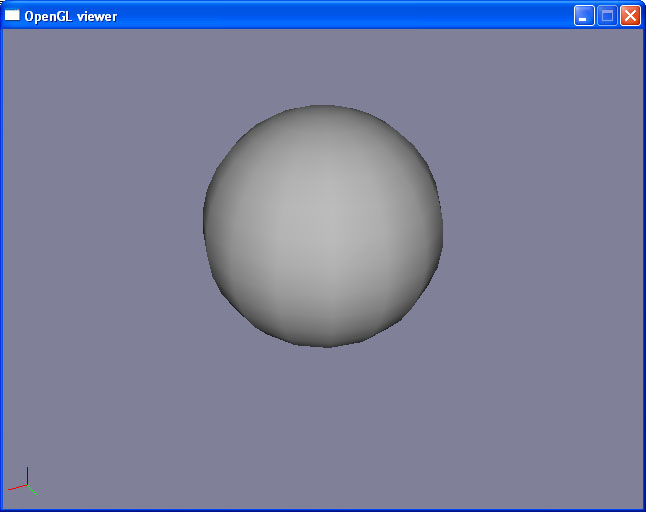
\includegraphics[width=8cm]{pics/helloworld}
\end{center}

The viewer tool reads the contents of the file which in this case
is an ordinary Python file and displays the scene using OpenGL.
When the input file is processed via the viewer tool it is executed
in a special environment where a couple of modules have already been imported.
That's why calling \code{Sphere()} doesn't result in a \exception{NameError}
exception. If you import the relevant modules yourself you can also call
the script without the viewer tool (however, you wouldn't get a visualization
of the scene then). You can also create the above scene directly in a 
Python shell:

\begin{verbatim}
>>> from cgkit.all import *
>>> Sphere()
<cgkit.quadrics.Sphere object at 0x051CC2D0>
\end{verbatim}

The first line imports all you need from cgkit which has to be done
manually now. The second line creates an instance of the
\class{Sphere} class. Usually, each object automatically inserts
itself into the scene, so we don't have to keep the resulting
reference. Now let's create another object:

\begin{verbatim}
>>> b=Box(name="Cube", pos=(1.5,2,0))
>>> listWorld()
Root
+---Cube (Box)
+---Sphere (Sphere)
\end{verbatim}

The first line creates a box object. This time we are passing a couple
of parameters like the object's name and its position and we store the
object in the variable \var{b} so we can manipulate the box afterwards.
The second line calls the \function{listWorld()} function
which prints a tree representation of the current scene.
Now it's time for a little nitpicking, actually the function only displays
the {\em world} (hence its name) and not the entire {\em scene}. The world
is what you see, it stores all 3D objects that have a visual representation
and is part of the scene. The whole scene also contains other objects
such as the timer, animation curves, etc. An object stored in the
scene is called a {\em component} and an object stored in the world
is, well, a {\em world object} (which is also a component as it is also
part of the scene). But back to the example. We have kept a reference to
the box, so let's see what we can do with it:

\begin{verbatim}
>>> b.name = "The Cube"
>>> listWorld()
Root
+---Sphere (Sphere)
+---The Cube (Box)
>>> b.pos
(1.5, 2, 0)
>>> b.pos=vec3(1,0,2)
>>> b.pos
(1, 0, 2)
>>> b.scale
(1, 1, 1)
\end{verbatim}

Every world object has a set of attributes that defines its state.
The exact set of attributes depends on the type of object, but there
are some common attributes that every world object has such as a name or
a position (see chapter \ref{worldobjects} for a reference of the available
world objects together with their attributes).

In the first example, we were only specifying one sphere with its default
attributes, that's why we had some geometry in the scene. But for a 3D scene
to be displayed you usually need two more ingredients: a camera and some 
light. In the above case, a default camera and light source was created
by the viewer tool. In the following example, we specify a complete scene,
including a camera, two colored light sources and a sphere with a material
assigned to it. Create a file "simplescene.py" with the following content:

\begin{verbatim}
TargetCamera(
    pos    = (3,2,2),
    target = (0,0,0)
)

GLPointLight(
    pos       = (3, -1, 2),
    diffuse   = (1, 0.7, 0.2)
)

GLPointLight(
    pos       = (-5, 3, 0),
    diffuse   = (0.2, 0.2, 0.5),
    intensity = 3.0
)

Sphere(
    name      = "My Sphere",
    radius    = 1.0,
    material  = GLMaterial(
                   diffuse = (0.7, 1, 0.7)
                )
)
\end{verbatim}

Display the scene by calling:

\begin{verbatim}
> viewer.py simplescene.py
\end{verbatim}

The result is this:

\begin{center}
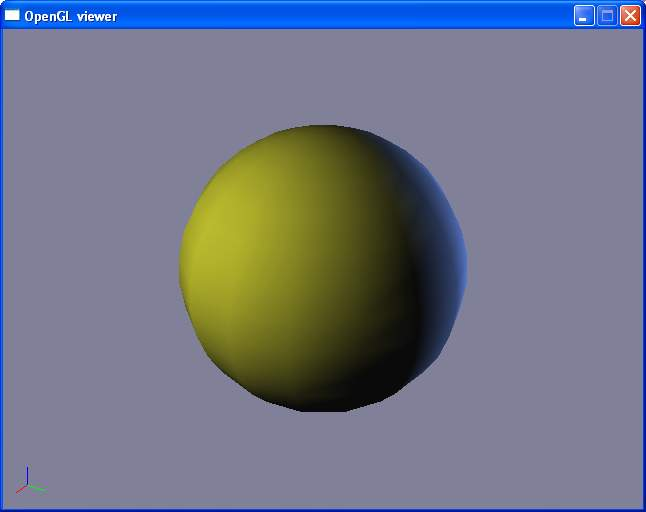
\includegraphics[width=8cm]{pics/simplescene1}
\end{center}

Using the \kbd{Alt} key in combination with the three mouse buttons
you can even navigate around in the scene (if you reach a pole
the camera position will jump around. This is because we are using
a \class{TargetCamera} that always tries to align its local "up"
direction with the global "up" direction, so this type of camera
can't be "upside down").

If you have a RenderMan renderer installed (there are free ones available
such as 3Delight, Aqsis or Pixie) you can try to visualize the above scene
with a different tool:

\begin{verbatim}
> render.py -r<renderer> simplescene.py
\end{verbatim}

\code{<renderer>} has to be replaced with either \code{3delight}, 
\code{aqsis} or \code{pixie}. 
This tool will display the same scene, but this time not using OpenGL but
the specified renderer. The result looks similar than before but is
much smoother:

\begin{center}
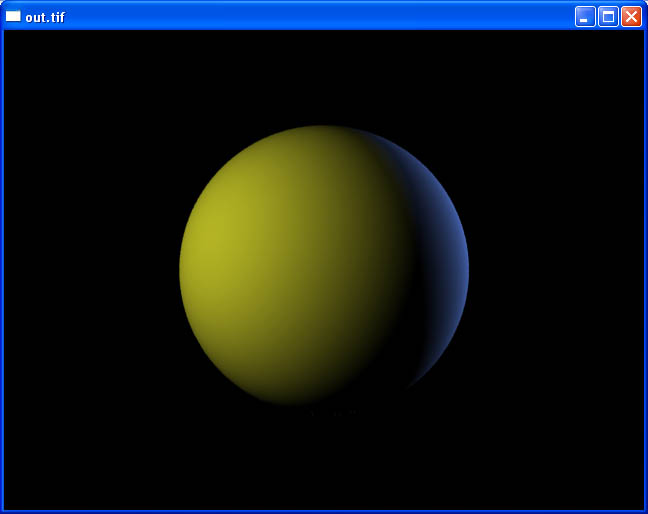
\includegraphics[width=8cm]{pics/simplescene2}
\end{center}

So if you want to create photorealistic images you can use the viewer tool
for previews and the render tool for creating the final image.

%----------------------------------------------------------------------
\section{Components and Slots}

This section gives an overview of the component framework that is the
basis for creating a dynamic 3D scene, i.e. one that is
animated/simulated. The basic mechanism is quite simple to understand
and you might already know it from other graphics packages as it is a
common concept in computer graphics software. The basic idea is to
have some black boxes that can generate values that vary with time and
that can be connected to the attributes we want to be animated. For
example, one such black box could output a three-dimensional vector
which could then be connected to the position of a teapot. If this
black box now produces a series of values that lie on a particular
curve we have an animation of a teapot traveling along that curve.

\begin{center}
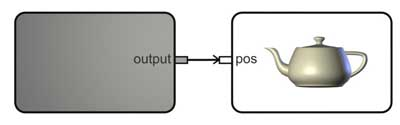
\includegraphics[width=10cm]{pics/slotexample}
\end{center}

In this package those black boxes and the teapot are called {\em
components}. A component is a container for {\em slots} which
represent the input or output values of their respective component. In
the above example, the output value of the "curve point generator" and
the position of the teapot are slots. You can also view them as
"animatable attributes" of an object if they mainly serve as input
values. Most slots can either serve as input value or output
value. However, if the value of a slot is actually computed by some
algorithm then this slot can only be used as output slot.

As a general rule, the actual slot corresponding to an attribute is
obtained by adding the suffix \code{_slot} to the attribute name.
Here is an example where two spheres s1 and s2 are created and
the position of s1 is connected to the position of s2 which means
s2 will always have the same position as s1:

\begin{verbatim}
>>> from cgkit import *
>>> s1=Sphere(pos=(1,2,3))
>>> s2=Sphere(pos=(-1,0,5))
>>> s1.pos
(1, 2, 3)
>>> s2.pos
(-1, 0, 5)

# Connect the positions 
>>> s1.pos_slot.connect(s2.pos_slot)

# Now s2 has the same position as s1
>>> s2.pos
(1, 2, 3)

# Changing the position of s1 will also change the position of s2
>>> s1.pos=vec3(-5,12,42)
>>> s2.pos
(-5, 12, 42)
\end{verbatim}

%----------------------------------------------------------------------
\section{Coordinate systems}

Each world object has a position and orientation in space. This
transformation can be described by a matrix that represents the
object's local coordinate system. The local coordinate system L stored
in each world object is given with respect to its parent coordinate
system which usually is just the world coordinate system unless you
have linked two objects. If you want the local coordinate system with
respect to the world system you have to travel up the transformation
hierarchy and concatenate all local systems (however, you don't have to
do that yourself as a world object already has an attribute 
\var{worldtransform} which does this for you). 

The geometry of a world object is given with respect to the local
coordinate system L. So this is the matrix that's required during
rendering. You get L by calling \method{localTransform()} on the
respective world object.

So far, if you would apply a rotation to an object it would rotate
around the origin or if you would scale the object the center of the
scale would lie in the origin. This is not always the desired behavior
and that's why you can specify a pivot point, or rather, a pivot
transformation or offset transformation P. This transformation is
given with respect to L and is the identity by default. You can get
and set this transformation using the \method{getOffsetTransform()} and
\method{setOffsetTransform()} methods.

The concatenation of L and P is the transformation T ($T=L\cdot
P$). This is what the
\var{transform}, \var{pos}, \var{rot} and \var{scale} slots of a world 
object describe. So if you modify the transform slot you also modify L
whereas P always remains constant, unless you change it explicitly via
\method{setOffsetTransform()}.

\begin{center}
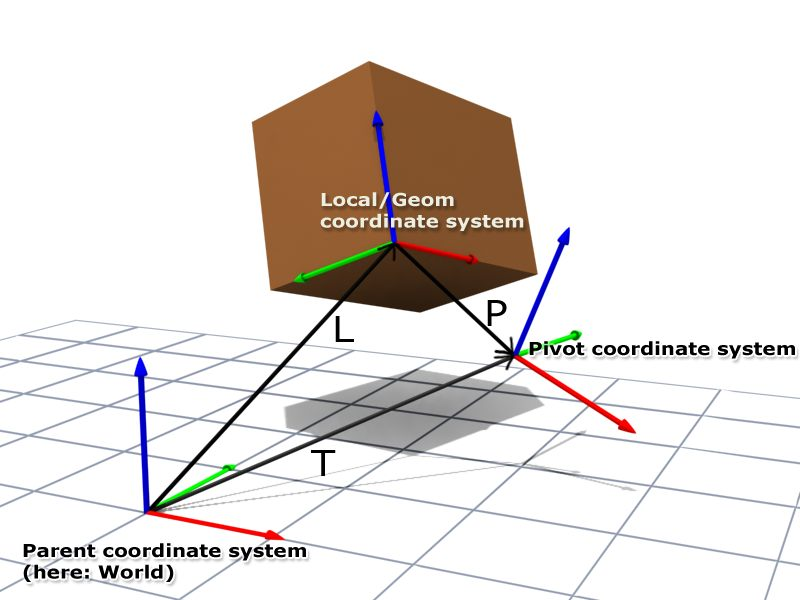
\includegraphics[width=12cm]{pics/coordsys}
\end{center}

Here is a simple code example where you can see the effects when
modifying the different transformations:

\begin{verbatim}
>>> s = Sphere()
>>> s.pos = vec3(1,2,0)
>>> s.pos
<1, 2, 0>
>>> s.setOffsetTransform(mat4().translation(vec3(2,4,7)))
>>> s.pos
<3, 6, 7>
>>> s.pos = vec3(0,0,0)
>>> s.pos
<0, 0, 0>
>>> s.localTransform()
[1, 0, 0, -2]
[0, 1, 0, -4]
[0, 0, 1, -7]
[0, 0, 0, 1]
\end{verbatim}

%---

\chapter{Building \& Installing \label{build}}

% Building and Installing

This chapter provides information about how to build the kit yourself
from the sources. You can skip this chapter if the kit is already
installed on your system or if you are installing binary versions.

%----------------------------------------------------------------------
\section{Building from the sources}

The following instructions will build and install the full version of cgkit.
You can also install the 'light' version by setting the variable 
\code{INSTALL_CGKIT_LIGHT} to \code{True} in your config file (just rename
the file \code{config_template.cfg} to \code{config.cfg} and uncomment the
corresponding line at the top of the file). Except for Python itself, 
installing the light version does not require any additional compiler, tool
or library, you simply have to call 

\begin{verbatim}
> python setup.py install    # that's all for the light version
\end{verbatim}

while being in the root directory of the cgkit sources. For installing
the light version you can skip the remainder of this section, but read
on if you actually want to install the full version.

The steps required to build the full version of the kit are the same
on every platform.  The build process assumes you have the following
tools/libraries installed on your system:

\begin{itemize}
\item \ulink{Boost}{http://www.boost.org/} (v1.31) - Make sure that Boost is
 installed including Boost.Python (e.g. Mac users who are using darwinports
 have to install the "+python" variant).
\item \ulink{SCons}{http://www.scons.org/} (v0.96.1)
\item \ulink{lib3ds}{http://lib3ds.sourceforge.net/} (v1.3.0) - {\bf Optional}. You need this if you want to import/export 3DS files.
\item \ulink{CyberX3D}{http://www.cybergarage.org/vrml/cx3d/cx3dcc/index.html} - {\bf Optional}. You need this if you want to import/export VRML or X3D files.
\item \ulink{OGRE}{http://www.ogre3d.org/} - {\bf Optional}. You need this if you want to use the OGRE-Viewer.
\item \ulink{STLport}{http://www.stlport.com/} - Only required on Windows when
 you want to use OGRE.
\item \ulink{3DxWare SDK}{http://www.3dconnexion.com/sdk.htm} - {\bf Optional} (currently Windows only). You need this if you want to use a SpaceMouse or SpaceBall.
\item \ulink{Wintab Programmer's Kit}{http://www.pointing.com/} - {\bf Optional} (Windows only). You need this if you want to use a tablet (or similar device).
\item \ulink{GloveSDK}{http://www.5dt.com/} - {\bf Optional}. You need this if you want to use a data glove. {\bf Note}: Download the version 2 SDK from the Ultra series, this can also be used with older gloves. You could also use version 1, but some functionality won't be available then.
\end{itemize}

If you have successfully installed the above tools and libraries you
can proceed with building the kit.The first step is to get the cgkit
sources. You can either download the source archive or check out the
latest version from CVS. The following build instructions apply to
both versions.

The package consists of three parts:

\begin{enumerate}
\item A pure C++ library that is independent of Python. This library is
 located in the \file{supportlib} directory.
\item Python wrappers around the above C++ library (using Boost.Python). 
 These wrappers are located in the \file{wrappers} directory.
\item The actual Python package using the wrappers. The package is located
 in the \file{cgkit} directory. The command line tools are in the main 
 directory.
\end{enumerate}

Part 2) and 3) is built and installed via the Python distutils (i.e.
the \file{setup.py} script). But before you can do so, you have to
build the C++ library manually using SCons.

{\bf Building the C++ support library:}

The C++ library is located in the directory \file{supportlib}. The library
uses SCons as its build system. If you have to customize the build process
you can create a file \file{cpp_config.cfg} where you can set some build
variables (e.g. adding search paths for include files). There is a template
file \file{cpp_config_template.cfg} which you can use to create the actual
config file. However, if you have installed every library in standard
directories it may well be that you don't need any config file at all.
Eventually you can build the library by calling \program{scons}:

\begin{verbatim}
> cd supportlib
> # ...create & modify cpp_config.cpp if necessary...
> scons
\end{verbatim}

If everything went fine you can see the result in the \file{lib}
subdirectory (\file{libcore.a} on Linux or \file{core.lib} on Windows).

{\bf Building the Python wrappers:}

The next step is to build and install the Python package. The package
uses the distutils, so you will find the familiar \file{setup.py}
script in the main directory. Customization of the build process can again
be done in a file called \file{config.cfg} which is executed by the setup
script. There is a template file \file{config_template.cfg} which you can
use to create your own config file. After setting up your
configuration you can install the package with the usual procedure:

\begin{verbatim}
> cd ..  # if you were still in the supportlib directory
> python setup.py install
\end{verbatim}

(see the manual \citetitle{Installing Python Modules} in your Python
documentation for more details about the distutils and how to proceed
if you have any special requirements)

Please also have a look at section \ref{externaldeps} for a list of
third-party packages you might have to install before you can use cgkit.
You can check cgkit and its dependencies with the script 
\file{utilities/checkenv.py} that is part of the source archive.
For a more thorough test you can run the unit tests in the \file{unittests}
directory.

A note to developers: You can build the package inplace by calling

\begin{verbatim}
> python setup.py build_ext --inplace
\end{verbatim}

In this case, the resulting binaries will be placed directly in the
\file{cgkit} directory which will then contain the entire package. Use
the \envvar{PYTHONPATH} variable and add the path to the main
directory if you want to use the inplace version from any other
directory.


%---

\chapter{Tools \label{tools}}

% Viewer tool

\section{The interactive viewer tool}

The tool \file{viewer.py} reads one or more files and displays the
scene using a simple OpenGL renderer. It creates events such as
keyboard, mouse or joystick events that can be used by the components
in the scene.

If the environment variable \envvar{VIEWER_DEFAULT_OPTIONS} exists, it
is read and parsed to set the default options. After that the options
in the command line are parsed.

{\bf Usage:}

\begin{verbatim}
viewer.py [options] inputfiles
\end{verbatim}

To exit the viewer press \kbd{Escape} or close the window. How to
navigate in the scene depends on the navigation mode (see option -N).

{\bf Options:}

\begin{description}
\item[\code{-f<int>} / \code{--fps=<int>}] 
Specifies the frame rate that should be tried to maintain while playing
back the scene (default: 30).

\item[\code{-h} / \code{--help}]
Print a help message.

\item[\code{-F} / \code{--full-screen}]
Open a full screen display.

\item[\code{-W<int>} / \code{--width=<int>}]
Specify the width in pixels of the window/screen (default: 640).

\item[\code{-H<int>} / \code{--height=<int>}]
Specify the height in pixels of the window/screen (default: 480). If
no height is specified it is computed based on the width and an aspect
ratio of 4/3.

\item[\code{-v} / \code{--verbose}]
Output info messages.

\item[\code{-p<str>} / \code{--plugin=<str>}]
If the argument specifies a file this file is loaded as a plugin, if it
is a directory, all files in this directory are loaded. You can specify
this option more than once or you can use a comma separated list of names.

You can also set files and paths via the environment variable
\envvar{CGKIT_PLUGIN_PATH}. The files/paths have to be separated either
by ':' or ';'.

\item[\code{-c<str>} / \code{--camera=<str>}]
Select the camera that should be used to view the scene. The argument
is the name of the camera. If no camera is specified the first camera
found in the scene is used.

\item[\code{-b<time>} / \code{--begin=<time>}]
Specify a time or frame where the animation/simulation should be started
(default: 0s). You can add the time unit such as 's' for seconds or 'f'
for frames. Frames are assumed if you don't specify a unit.

\item[\code{-e<time>} / \code{--end=<time>}]
Specify a time or frame where the animation/simulation should be stopped.
You can add the time unit such as 's' for seconds or 'f' for frames. 
Frames are assumed if you don't specify a unit.

\item[\code{-U<axis>} / \code{--up=<axis>}]
Specify the default value for the up axis. The argument may be either
'y' or 'z'.

\item[\code{-O<str>} / \code{--option=<str>}]
Add a global option that will be stored in the scene. The argument should
have the form "name=value". Using this option is equivalent to writing
"Globals( name=value )" in a scene file.

\item[\code{-t} / \code{--set-time}]
Set the starting time directly instead of stepping there from time 0.

\item[\code{-S<str>} / \code{--stereo=<str>}]
Activate stereo display. The argument specifies the method that should be
used to create a stereo image. It can be either \var{vsplit} or \var{glstereo}.

\item[\code{-D<float>} / \code{--eye-distance=<float>}]
Default eye distance for stereo display (default 0.07). This distance
value is used if the camera does not explicitly specify a distance value
(i.e. if it has no attribute \var{eye_distance}).

\item[\code{-B} / \code{--bounding-box}]
Display the bounding boxes.

\item[\code{-P<str>} / \code{--polygon-mode=<str>}]
Specify how polygons should be rendered. Possible values are
\var{fill} (default), \var{line} and \var{point}.

\item[\code{-s<str>} / \code{--save=<str>}]
When this option is specified each frame is saved under the given name
(+ frame number). The extension determines the image format.

\item[\code{-N<str>} / \code{--navigation-mode=<str>}]
Specify which navigation mode to activate. The viewer can emulate the
navigation of a few common 3D packages. Possible values are
\var{Maya} (default), \var{MAX} and \var{Softimage} (case-insensitive).

In Maya mode you navigate by pressing the \kbd{Alt} key in combination
with any of the three mouse buttons. In MAX mode you press the middle
mouse button either alone or in combination with \kbd{Alt} or \kbd{Control}
and \kbd{Alt}. In Softimage mode, only the Softimage Navigation Tool is
emulated (it's as if this tool is permanently active), i.e. you navigate
by using one of the three mouse buttons.

\item[\code{-X} / \code{--disable-spacedevice}]
Disables support for SpaceMouse/SpaceBall. This option can be used if there
are any problems with the driver or initialization takes too long.

\item[\code{-T} / \code{--disable-wintab}]
Disables tablet support. This option can be used if there are any
problems with the driver or initialization takes too long.

\end{description}

{\bf Events:}

The viewer tool generates the following user input events (see the
module \refmodule{cgkit.events} for more details about these events):

\begin{itemize}
\item \code{KEY_PRESS}
\item \code{KEY_RELEASE}
\item \code{LEFT_DOWN}
\item \code{MIDDLE_DOWN}
\item \code{RIGHT_DOWN}
\item \code{MOUSE_BUTTON_DOWN}
\item \code{LEFT_UP}
\item \code{MIDDLE_UP}
\item \code{RIGHT_UP}
\item \code{MOUSE_BUTTON_UP}
\item \code{MOUSE_WHEEL}
\item \code{MOUSE_MOVE}
\item \code{JOYSTICK_AXIS}
\item \code{JOYSTICK_BALL}
\item \code{JOYSTICK_HAT}
\item \code{JOYSTICK_BUTTON_DOWN}
\item \code{JOYSTICK_BUTTON_UP}
\item \code{SPACE_MOTION}
\item \code{SPACE_BUTTON_DOWN}
\item \code{SPACE_BUTTON_UP}
\item \code{SPACE_BUTTON_ZERO}
\item \code{TABLET}
\end{itemize}

{\bf Timing:}

The operations per frame are as follows (in this order):

\begin{enumerate}
\item Render and display the current scene at time $t$
\item Handle events
\item Step frame (i.e. increase the time by $\Delta t$ and signal the
  \code{STEP_FRAME} event)
\item Sync to the specified framerate
\end{enumerate}

% Render tool

\section{The render tool}

The tool \file{render.py} reads one or more files and renders the
scene using a RenderMan renderer. The tool takes care of creating the
RIB files and the shaders, compiling the shaders and launching the 
renderer.

If the environment variable \envvar{RENDER_DEFAULT_OPTIONS} exists, it
is read and parsed to set the default options. After that the options
in the command line are parsed.

{\bf Usage:}

\begin{verbatim}
render.py [options] inputfiles
\end{verbatim}


{\bf Options:}

\begin{description}
\item[\code{-f<int>} / \code{--fps=<int>}] 
Specifies the number of frames per second (default: 30).

\item[\code{-h} / \code{--help}]
Print a help message.

\item[\code{-W<int>} / \code{--width=<int>}]
Specify the width in pixels of the window/screen (default: 640).

\item[\code{-H<int>} / \code{--height=<int>}]
Specify the height in pixels of the window/screen (default: 480). If
no height is specified it is computed based on the width and an aspect
ratio of 4/3.

\item[\code{-v} / \code{--verbose}]
Output info messages.

\item[\code{-p<str>} / \code{--plugin=<str>}]
If the argument specifies a file this file is loaded as a plugin, if it
is a directory, all files in this directory are loaded. You can specify
this option more than once or you can use a comma separated list of names.

You can also set files and paths via the environment variable
\envvar{CGKIT_PLUGIN_PATH}. The files/paths have to be separated either
by ':' or ';'.

\item[\code{-c<str>} / \code{--camera=<str>}]
Select the camera that should be used to view the scene. The argument
is the name of the camera. If no camera is specified the first camera
found in the scene is used.

\item[\code{-b<time>} / \code{--begin=<time>}]
Specify a time or frame where the animation/simulation should be started
(default: 0s). You can add the time unit such as 's' for seconds or 'f'
for frames. Frames are assumed if you don't specify a unit.

\item[\code{-e<time>} / \code{--end=<time>}]
Specify a time or frame where the animation/simulation should be stopped.
You can add the time unit such as 's' for seconds or 'f' for frames. 
Frames are assumed if you don't specify a unit.

\item[\code{-U<axis>} / \code{--up=<axis>}]
Specify the default value for the up axis. The argument may be either
'y' or 'z'.

\item[\code{-O<str>} / \code{--option=<str>}]
Add a global option that will be stored in the scene. The argument should
have the form "name=value". Using this option is equivalent to writing
"Globals( name=value )" in a scene file.

\item[\code{-t} / \code{--set-time}]
Set the starting time directly instead of stepping there from time 0.

\item[\code{-r<str>} / \code{--renderer=<str>}]
Select the renderer to use (you can choose among \code{aqsis},
\code{3delight}, \code{pixie}, \code{prman}, \code{air} and \code{rdc}).

\item[\code{-I<str>} / \code{--include=<str>}]
Add the specified include path to the list of paths used for compiling
the shaders.

\item[\code{-B} / \code{--bake}]
Activate texture baking mode.

\end{description}

{\bf Events:}

The render tool does not generate any user input events.


%---

\chapter{Generic modules \label{modules1}}

\localmoduletable

\section{\module{cgkitinfo} ---
         Release information}

\declaremodule{extension}{cgkit.cgkitinfo}
\modulesynopsis{Provides version information.}

New in version 1.1. This module contains two variables that carry
information about the version of the kit.

\begin{datadesc}{version}
A string containing version information of this release.
\end{datadesc}

\begin{datadesc}{version_info}
A 4-tuple (\var{major}, \var{minor}, \var{micro}, \var{releaselevel})
containing the components of the version number. The first three
values are integers, whereas \var{releaselevel} is a string containing
"cvs", "alpha", "beta" or "final".
\end{datadesc}

\section{\module{cgtypes} ---
         Vectors, matrices and quaternions}

\declaremodule{extension}{cgkit.cgtypes}
\modulesynopsis{Basic types useful for computer graphics.}

This module contains the fundamental types which make working with 3D
data much easier. The types are:

\begin{itemize}
\item vec3 -- a three dimensional vector type to store points, vectors, normals or even colors.
\item vec4 -- a four dimensional vector type to store homogenous points, for example.
\item mat3 -- a 3x3 matrix to store linear transformations.
\item mat4 -- a 4x4 matrix to store affine transformations.
\item quat -- a quaternion type as a specialized way to store rotations.
\end{itemize}

You import all of those types at once with

\begin{verbatim}
from cgkit.cgtypes import *
\end{verbatim}

or you can import them individually like this

\begin{verbatim}
from cgkit.cgtypes import vec3, mat4
\end{verbatim}

In general, you can use those types just as if they were built-in
types which means the mathematical operators can be used and have
their respective meaning. Each type has some additional methods which
are described in the respective documentation.

Here are some examples:

\begin{verbatim}
>>> from cgkit.cgtypes import *
>>> v=vec3(0.5,1.0,-2.5)
>>> print v
(0.5000, 1.0000, -2.5000)
>>> print v.length()
2.73861278753
>>> v=v.normalize()
>>> print v
(0.1826, 0.3651, -0.9129)
>>> print v.length()
1.0
\end{verbatim}

Now let's construct a rotation matrix that rotates points by 90
degrees around the z-axis:

\begin{verbatim}
>>> M=mat4(1).rotate(0.5*math.pi, vec3(0,0,1))
\end{verbatim}

and apply the rotation to the vector (1,0,0) (the x-axis):

\begin{verbatim}
>>> print M*vec3(1,0,0)
(0.0000, 1.0000, 0.0000)
\end{verbatim}

The module contains the following functions:

\begin{funcdesc}{getEpsilon}{}
Return the epsilon threshold which is used for doing comparisons.
\end{funcdesc}

\begin{funcdesc}{setEpsilon}{eps}
Sets a new epsilon threshold and returns the previously set value. Two
values are considered to be equal if their absolute difference is less
than or equal to epsilon.
\end{funcdesc}

\begin{funcdesc}{slerp}{t, q0, q1}
Performs a spherical linear interpolation between two quaternions q0
and q1. For t=0.0 the return value equals q0, for t=1.0 it equals
q1. q0 and q1 must be unit quaternions. \\
New in version 1.1.
\end{funcdesc}

\begin{funcdesc}{squad}{t, a, b, c, d}
Performs a spherical cubic interpolation between quaternion a and d
where quaternion b and c define the shape of the interpolation
curve. For t=0.0 the return value equals a, for t=1.0 it equals d. All
quaternions must be unit quaternions. \\
New in version 1.1.
\end{funcdesc}

%----------------------------------------------------------------------
\subsection{vec3 - 3d vector}
\label{vec3}

A \class{vec3} represents a 3D vector type that can be used to store
points, vector, normals or even colors. You can construct a
\class{vec3} by several ways:

\begin{verbatim}
# all components are set to zero
v = vec3()

-> (0.0000, 0.0000, 0.0000)

# set all components to one value
v = vec3(2.5)

-> (2.5000, 2.5000, 2.5000)

# set a 2d vector, the 3rd component will be zero
v = vec3(1.5, 0.8)

-> (1.5000, 0.8000, 0.0000)

# initialize all three components
v = vec3(1.5, 0.8, -0.5)

-> (1.5000, 0.8000, -0.5000)
\end{verbatim}

Additionally you can use all of the above, but store the values inside
a tuple, a list or a string:

\begin{verbatim}
v = vec3([1.5, 0.8, -0.5])
w = vec3("1.5, 0.8")
\end{verbatim}

Finally, you can initialize a vector with a copy of another vector:

\begin{verbatim}
v = vec3(w)
\end{verbatim}

A \class{vec3} can be used just like a list with 3 elements, so you
can read and write components using the index operator or by accessing
the components by name:

\begin{verbatim}
>>> v=vec3(1,2,3)
>>> print v[0]
1.0
>>> print v.y
2.0
\end{verbatim}

%----------------------------------------
{\bf Mathematical operations}

The mathematical operators are supported with the following
combination of types:

\begin{verbatim}
vec3  =  vec3 + vec3
vec3  =  vec3 - vec3
float =  vec3 * vec3      # dot product
vec3  = float * vec3
vec3  =  vec3 * float
vec3  =  vec3 / float
vec3  =  vec3 % float     # each component
vec3  =  vec3 % vec3      # component wise
vec3  = -vec3
float =  vec3[i]          # get or set element
\end{verbatim}

Additionally, you can compare vectors with \code{==}, \code{!=}, \code{<}, 
\code{<=}, \code{>}, \code{>=}. Each
comparison (except \code{<} and \code{>}) takes an epsilon environment
into account, this means two values are considered to be equal if
their absolute difference is less than or equal to a threshold value
epsilon. You can read and write this threshold value using the
functions \function{getEpsilon()} and \function{setEpsilon()}.

Taking the absolute value of a vector will return the length of the vector: 

\begin{verbatim}
float = abs(v)            # this is equivalent to v.length()
\end{verbatim}

%----------------------------------------
{\bf Methods}

\begin{methoddesc}{angle}{other}
Return angle (in radians) between \var{self} and \var{other}.
\end{methoddesc}

\begin{methoddesc}{cross}{other}
Return cross product of \var{self} and \var{other}.
\end{methoddesc}

\begin{methoddesc}{length}{}
Returns the length of the vector ($\sqrt{x^2+y^2+z^2}$). This is
equivalent to calling \code{abs(self)}.
\end{methoddesc}

\begin{methoddesc}{normalize}{}
Returns normalized vector. If the method is called on the null vector
(where each component is zero) a \exception{ZeroDivisionError} is raised.
\end{methoddesc}

\begin{methoddesc}{reflect}{N}
Returns the reflection vector. \var{N} is the surface normal which has to be
of unit length.
\end{methoddesc}

\begin{methoddesc}{refract}{N, eta}
Returns the transmitted vector. \var{N} is the surface normal which has to
be of unit length. \var{eta} is the relative index of refraction. If the
returned vector is zero then there is no transmitted light because of
total internal reflection.
\end{methoddesc}

\begin{methoddesc}{ortho}{}
Returns a vector that is orthogonal to \var{self} (where
\code{self*self.ortho()==0}).
\end{methoddesc}

\begin{methoddesc}{min}{}
Returns the minimum value of the components.
\end{methoddesc}

\begin{methoddesc}{max}{}
Returns the maximum value of the components.
\end{methoddesc}

\begin{methoddesc}{minIndex}{}
Return the index of the component with the minimum value.
\end{methoddesc}

\begin{methoddesc}{maxIndex}{}
Return the index of the component with the maximum value.
\end{methoddesc}

\begin{methoddesc}{minAbs}{}
Returns the minimum absolute value of the components.
\end{methoddesc}

\begin{methoddesc}{maxAbs}{}
Returns the maximum absolute value of the components.
\end{methoddesc}

\begin{methoddesc}{minAbsIndex}{}
Return the index of the component with the minimum absolute value.
\end{methoddesc}

\begin{methoddesc}{maxAbsIndex}{}
Return the index of the component with the maximum absolute value.
\end{methoddesc}


%----------------------------------------------------------------------
\subsection{vec4 - 4d vector}
\label{vec4}

A \class{vec4} represents a 4D vector type. You can construct a \class{vec4}
by several ways:

\begin{verbatim}
# all components are set to zero
v = vec4()

-> (0.0000, 0.0000, 0.0000, 0.0000)

# set all components to one value
v = vec4(2.5)

-> (2.5000, 2.5000, 2.5000, 2.5000)

# set a 2d vector, the ramaining components will be zero
v = vec4(1.5, 0.8)

-> (1.5000, 0.8000, 0.0000, 0.0000)

# set a 3d vector, the ramaining component will be zero
v = vec4(1.5, 0.8, -0.5)

-> (1.5000, 0.8000, -0.5000, 0.0000)

# set all components
v = vec4(1.5, 0.8, -0.5, 0.2)

-> (1.5000, 0.8000, -0.5000, 0.2000)
\end{verbatim}

Additionally you can use all of the above, but store the values inside
a tuple, a list or a string:

\begin{verbatim}
v = vec4([1.5, 0.8, -0.5])
w = vec4("1.5, 0.8")
\end{verbatim}

Finally, you can initialize a vector with a copy of another vector:

\begin{verbatim}
v = vec4(w)
\end{verbatim}

A \class{vec4} can be used just like a list with 4 elements, so you
can read and write components using the index operator or by accessing
the components by name:

\begin{verbatim}
>>> v=vec4(1,2,3,1)
>>> print v[0]
1.0
>>> print v.y
2.0
>>> print v.w
1.0
>>> print v.t   # this is the same as v.w
1.0
\end{verbatim}

The 4th component can be accessed either by the name \code{w} or
\code{t}. You might prefer the former name when using the vector as a
homogenous coordinate while the latter might be preferable when the
4th component shall represent a time value.

%----------------------------------------
{\bf Mathematical operations}

The mathematical operators are supported with the following
combination of types:

\begin{verbatim}
vec4  =  vec4 + vec4
vec4  =  vec4 - vec4
float =  vec4 * vec4      # dot product
vec4  = float * vec4
vec4  =  vec4 * float
vec4  =  vec4 / float
vec4  =  vec4 % float     # each component
vec4  =  vec4 % vec4      # component wise
vec4  = -vec4
float =  vec4[i]          # get or set element
\end{verbatim}

Additionally, you can compare vectors with \code{==}, \code{!=}, \code{<}, 
\code{<=}, \code{>}, \code{>=}. Each
comparison (except \code{<} and \code{>}) takes an epsilon environment
into account, this means two values are considered to be equal if
their absolute difference is less than or equal to a threshold value
epsilon. You can read and write this threshold value using the
functions \function{getEpsilon()} and \function{setEpsilon()}.

Taking the absolute value of a vector will return the length of the vector: 

\begin{verbatim}
float = abs(v)            # this is equivalent to v.length()
\end{verbatim}

%----------------------------------------
{\bf Methods}

\begin{methoddesc}{length}{}
Returns the length of the vector ($\sqrt{x^2+y^2+z^2}$). This is
equivalent to calling \code{abs(self)}.
\end{methoddesc}

\begin{methoddesc}{normalize}{}
Returns normalized vector. If the method is called on the null vector
(where each component is zero) a \exception{ZeroDivisionError} is raised.
\end{methoddesc}




%----------------------------------------------------------------------
\subsection{mat3 - 3x3 matrix}
\label{mat3}

A \class{mat3} represents a 3x3 matrix which can be used to store
linear transformations (if you want to store translations or
perspective transformations, you have to use a \class{mat4}). You can
construct a \class{mat3} in several ways:

\begin{verbatim}
# all components are set to zero
M = mat3()

[   0.0000,    0.0000,    0.0000]
[   0.0000,    0.0000,    0.0000]
[   0.0000,    0.0000,    0.0000]

# identity matrix
M = mat3(1.0)

[   1.0000,    0.0000,    0.0000]
[   0.0000,    1.0000,    0.0000]
[   0.0000,    0.0000,    1.0000]

# The elements on the diagonal are set to 2.5
M = mat3(2.5)

[   2.5000,    0.0000,    0.0000]
[   0.0000,    2.5000,    0.0000]
[   0.0000,    0.0000,    2.5000]

# All elements are explicitly set (values must be given in row-major order)
M = mat3(a,b,c,d,e,f,g,h,i)
M = mat3([a,b,c,d,e,f,g,h,i])

[ a, b, c]
[ d, e, f]
[ g, h, i]

# Create a copy of matrix N (which also has to be a mat3)
M = mat3(N)

# Specify the 3 columns of the matrix (as vec3's or sequences with 3 elements)
M = mat3(a,b,c)

[ a[0], b[0], c[0] ]
[ a[1], b[1], c[1] ]
[ a[2], b[2], c[2] ]

# All elements are explicitly set and are stored inside a string
M = mat3("1,2,3,4,5,6,7,8,9")

[   1.0000,    2.0000,    3.0000]
[   4.0000,    5.0000,    6.0000]
[   7.0000,    8.0000,    9.0000]
\end{verbatim}

%----------------------------------------
{\bf Mathematical operations}

The mathematical operators are supported with the following
combination of types:

\begin{verbatim}
mat3  =  mat3 + mat3
mat3  =  mat3 - mat3
mat3  =  mat3 * mat3
vec3  =  mat3 * vec3
vec3  =  vec3 * mat3
mat3  = float * mat3
mat3  =  mat3 * float
mat3  =  mat3 / float
mat3  =  mat3 % float     # each component
mat3  = -mat3
vec3  =  mat3[i]          # get or set column i (as vec3)
float =  mat3[i,j]        # get or set element in row i and column j
\end{verbatim}

Additionally, you can compare matrices with \code{==} and \code{!=}.

%----------------------------------------
{\bf Methods}

\begin{methoddesc}{getColumn}{index}
Return column index (0-based) as a \class{vec3}.
\end{methoddesc}

\begin{methoddesc}{setColumn}{index, value}
Set column index (0-based) to \var{value} which has to be a sequence
of 3 floats (this includes \class{vec3}).
\end{methoddesc}

\begin{methoddesc}{getRow}{index}
Return row index (0-based) as a \class{vec3}.
\end{methoddesc}

\begin{methoddesc}{setRow}{index, value}
Set row index (0-based) to \var{value} which has to be a sequence of
3 floats (this includes \class{vec3}).
\end{methoddesc}

\begin{methoddesc}{getDiag}{}
Return the diagonal as a \class{vec3}.
\end{methoddesc}

\begin{methoddesc}{setDiag}{value}
Set the diagonal to \var{value} which has to be a sequence of
3 floats (this includes \class{vec3}).
\end{methoddesc}

\begin{methoddesc}{toList}{rowmajor=False}
Returns a list containing the matrix elements. By default, the list is
in column-major order. If you set the optional argument \var{rowmajor} to
\code{True}, you'll get the list in row-major order.
\end{methoddesc}

\begin{methoddesc}{identity}{}
Returns the identity matrix. 
\end{methoddesc}

\begin{methoddesc}{transpose}{}
Returns the transpose of the matrix.
\end{methoddesc}

\begin{methoddesc}{determinant}{}
Returns the determinant of the matrix.
\end{methoddesc}

\begin{methoddesc}{inverse}{}
Returns the inverse of the matrix.
\end{methoddesc}

\begin{methoddesc}{scaling}{s}
Returns a scaling transformation. The scaling vector \var{s} must be a
3-sequence (e.g. a \class{vec3}).

\[ \left( \begin{array}{ccc}
s.x & 0 & 0 \\
0 & s.y & 0 \\
0 & 0 & s.z \\
\end{array} \right) \]
\end{methoddesc}

\begin{methoddesc}{rotation}{angle, axis}
Returns a rotation transformation. The angle must be given in radians,
\var{axis} has to be a 3-sequence (e.g. a \class{vec3}).
\end{methoddesc}

\begin{methoddesc}{scale}{s}
Concatenates a scaling transformation and returns \var{self}. The scaling
vector s must be a 3-sequence (e.g. a \class{vec3}).
\end{methoddesc}

\begin{methoddesc}{rotate}{angle, axis}
Concatenates a rotation transformation and returns \var{self}. The angle
must be given in radians, axis has to be a 3-sequence (e.g. a \class{vec3}).
\end{methoddesc}

\begin{methoddesc}{ortho}{}
Returns a matrix with orthogonal base vectors.
\end{methoddesc}

\begin{methoddesc}{decompose}{}
Decomposes the matrix into a rotation and scaling part. The method
returns a tuple (rotation, scaling). The scaling part is given as a
\class{vec3}, the rotation is still a \class{mat3}.
\end{methoddesc}

\begin{methoddesc}{fromEulerXYZ}{x, y, z}
Initializes a rotation matrix from Euler angles. \var{x} is the angle
around the x axis, \var{y} the angle around the y axis and \var{z} the
angle around the z axis. All angles must be given in radians. The order
of the individual rotations is X-Y-Z (where each axis refers to the {\em
local} axis, i.e. the first rotation is about the x axis which rotates
the Y and Z axis, then the second rotation is about the rotated Y axis 
and so on).
\end{methoddesc}

\begin{methoddesc}{fromEulerYZX}{x, y, z}
See above. The order is YZX.
\end{methoddesc}

\begin{methoddesc}{fromEulerZXY}{x, y, z}
See above. The order is ZXY.
\end{methoddesc}

\begin{methoddesc}{fromEulerXZY}{x, y, z}
See above. The order is XZY.
\end{methoddesc}

\begin{methoddesc}{fromEulerYXZ}{x, y, z}
See above. The order is YXZ.
\end{methoddesc}

\begin{methoddesc}{fromEulerZYX}{x, y, z}
See above. The order is ZYX.
\end{methoddesc}

\begin{methoddesc}{toEulerXYZ}{}
Return the Euler angles of a rotation matrix. The order is XYZ.
\end{methoddesc}

\begin{methoddesc}{toEulerYZX}{}
Return the Euler angles of a rotation matrix. The order is YZX.
\end{methoddesc}

\begin{methoddesc}{toEulerZXY}{}
Return the Euler angles of a rotation matrix. The order is ZXY.
\end{methoddesc}

\begin{methoddesc}{toEulerXZY}{}
Return the Euler angles of a rotation matrix. The order is XZY.
\end{methoddesc}

\begin{methoddesc}{toEulerYXZ}{}
Return the Euler angles of a rotation matrix. The order is YXZ.
\end{methoddesc}

\begin{methoddesc}{toEulerZYX}{}
Return the Euler angles of a rotation matrix. The order is ZYX.
\end{methoddesc}


%----------------------------------------------------------------------
\subsection{mat4 - 4x4 matrix}
\label{mat4}

A \class{mat4} represents a 4x4 matrix which can be used to store
transformations. You can construct a \class{mat4} in several ways:

\begin{verbatim}
# all components are set to zero
M = mat4()

[   0.0000,    0.0000,    0.0000,    0.0000]
[   0.0000,    0.0000,    0.0000,    0.0000]
[   0.0000,    0.0000,    0.0000,    0.0000]
[   0.0000,    0.0000,    0.0000,    0.0000]

# identity matrix
M = mat4(1.0)

[   1.0000,    0.0000,    0.0000,    0.0000]
[   0.0000,    1.0000,    0.0000,    0.0000]
[   0.0000,    0.0000,    1.0000,    0.0000]
[   0.0000,    0.0000,    0.0000,    1.0000]

# The elements on the diagonal are set to 2.5
M = mat4(2.5)

[   2.5000,    0.0000,    0.0000,    0.0000]
[   0.0000,    2.5000,    0.0000,    0.0000]
[   0.0000,    0.0000,    2.5000,    0.0000]
[   0.0000,    0.0000,    0.0000,    2.5000]

# All elements are explicitly set (values must be given in row-major order)
M = mat4(a,b,c,d,e,f,g,h,i,j,k,l,m,n,o,p)
M = mat4([a,b,c,d,e,f,g,h,i,j,k,l,m,n,o,p])

[ a, b, c, d ]
[ e, f, g, h ]
[ i, j, k, l ]
[ m, n, o, p ]

# Create a copy of matrix N (which also has to be a mat4)
M = mat4(N)

# Specify the 4 columns of the matrix (as vec4's or sequences with 4 elements)
M = mat4(a,b,c,d)

[ a[0], b[0], c[0], d[0] ]
[ a[1], b[1], c[1], d[1] ]
[ a[2], b[2], c[2], d[2] ]
[ a[3], b[3], c[3], d[3] ]

# All elements are explicitly set and are stored inside a string
M = mat4("1,2,3,4,5,6,7,8,9,10,11,12,13,14,15,16")

[   1.0000,    2.0000,    3.0000,    4.0000]
[   5.0000,    6.0000,    7.0000,    8.0000]
[   9.0000,   10.0000,   11.0000,   12.0000]
[  13.0000,   14.0000,   15.0000,   16.0000]
\end{verbatim}

%----------------------------------------
{\bf Mathematical operations}

The mathematical operators are supported with the following
combination of types:

\begin{verbatim}
mat4  =  mat4 + mat4
mat4  =  mat4 - mat4
mat4  =  mat4 * mat4
vec4  =  mat4 * vec4
vec4  =  vec4 * mat4
vec3  =  mat4 * vec3      # missing coordinate in vec3 is implicitly set to 1.0
vec3  =  vec3 * mat4      # missing coordinate in vec3 is implicitly set to 1.0
mat4  = float * mat4
mat4  =  mat4 * float
mat4  =  mat4 / float
mat4  =  mat4 % float     # each component
mat4  = -mat4
vec4  =  mat4[i]          # get or set column i (as vec4)
float =  mat4[i,j]        # get or set element in row i and column j
\end{verbatim}

Additionally, you can compare matrices with \code{==} and \code{!=}.

%----------------------------------------
{\bf Methods}

\begin{methoddesc}{getColumn}{index}
Return column index (0-based) as a \class{vec4}.
\end{methoddesc}

\begin{methoddesc}{setColumn}{index, value}
Set column index (0-based) to \var{value} which has to be a sequence
of 4 floats (this includes \class{vec4}).
\end{methoddesc}

\begin{methoddesc}{getRow}{index}
Return row index (0-based) as a \class{vec4}.
\end{methoddesc}

\begin{methoddesc}{setRow}{index, value}
Set row index (0-based) to \var{value} which has to be a sequence of
4 floats (this includes \class{vec4}).
\end{methoddesc}

\begin{methoddesc}{getDiag}{}
Return the diagonal as a \class{vec4}.
\end{methoddesc}

\begin{methoddesc}{setDiag}{value}
Set the diagonal to \var{value} which has to be a sequence of
4 floats (this includes \class{vec4}).
\end{methoddesc}

\begin{methoddesc}{toList}{rowmajor=False}
Returns a list containing the matrix elements. By default, the list is
in column-major order (which can be directly used in OpenGL or RenderMan). 
If you set the optional argument \var{rowmajor} to
\code{True}, you will get the list in row-major order.
\end{methoddesc}

\begin{methoddesc}{identity}{}
Returns the identity matrix. 
\end{methoddesc}

\begin{methoddesc}{transpose}{}
Returns the transpose of the matrix.
\end{methoddesc}

\begin{methoddesc}{determinant}{}
Returns the determinant of the matrix.
\end{methoddesc}

\begin{methoddesc}{inverse}{}
Returns the inverse of the matrix.
\end{methoddesc}

\begin{methoddesc}{translation}{t}
Returns a translation transformation. The translation vector t must be a
3-sequence (e.g. a vec3).

\[ \left( \begin{array}{cccc}
1 & 0 & 0 & t.x \\
0 & 1 & 0 & t.x \\
0 & 0 & 1 & t.x \\
0 & 0 & 0 & 1 
\end{array} \right) \]

\end{methoddesc}

\begin{methoddesc}{scaling}{s}
Returns a scaling transformation. The scaling vector \var{s} must be a
3-sequence (e.g. a \class{vec3}).

\[ \left( \begin{array}{cccc}
s.x & 0 & 0 & 0\\
0 & s.y & 0 & 0\\
0 & 0 & s.z & 0\\
0 & 0 & 0 & 1\\
\end{array} \right) \]
\end{methoddesc}

\begin{methoddesc}{rotation}{angle, axis}
Returns a rotation transformation. The angle must be given in radians,
\var{axis} has to be a 3-sequence (e.g. a \class{vec3}).
\end{methoddesc}

\begin{methoddesc}{translate}{t}
Concatenate a translation transformation and return \var{self}. The
translation vector \var{t} must be a 3-sequence (e.g. a \class{vec3}).
\end{methoddesc}

\begin{methoddesc}{scale}{s}
Concatenates a scaling transformation and returns \var{self}. The scaling
vector s must be a 3-sequence (e.g. a \class{vec3}).
\end{methoddesc}

\begin{methoddesc}{rotate}{angle, axis}
Concatenates a rotation transformation and returns \var{self}. The angle
must be given in radians, axis has to be a 3-sequence (e.g. a \class{vec3}).
\end{methoddesc}

\begin{methoddesc}{frustum}{left, right, bottom, top, near, far}
Returns a matrix that represents a perspective depth
transformation. This method is equivalent to the OpenGL command
\cfunction{glFrustum()}.

\note{If you want to use this transformation in RenderMan, keep in
mind that the RenderMan camera is looking in the positive z direction
whereas the OpenGL camera is looking in the negative direction.}
\end{methoddesc}

\begin{methoddesc}{perspective}{fovy, aspect, near, far}
Similarly to \method{frustum()} this method returns a perspective
transformation, the only difference is the meaning of the input
parameters. The method is equivalent to the OpenGL command
\cfunction{gluPerspective()}.
\end{methoddesc}

\begin{methoddesc}{orthographic}{left, right, bottom, top, near, far}
Returns a matrix that represents an orthographic transformation. This
method is equivalent to the OpenGL command \cfunction{glOrtho()}.
\end{methoddesc}

\begin{methoddesc}{lookAt}{pos, target, up=(0,0,1)}
Returns a transformation that moves the coordinate system to position
\var{pos} and rotates it so that the z-axis points onto point
\var{target}. The y-axis is pointing as closely as possible into the
same direction as \var{up}. All three parameters have to be a
3-sequence.

You can use this transformation to position objects in the scene that
have to be oriented towards a particular point. Or you can use it to
position the camera in the virtual world. In this case you have to
take the inverse of this transformation as viewport transformation (to
convert world space coordinates into camera space coordinates).
\end{methoddesc}

\begin{methoddesc}{ortho}{}
Returns a matrix with orthogonal base vectors. The x-, y- and z-axis
are made orthogonal. The fourth column and row remain untouched.
\end{methoddesc}

\begin{methoddesc}{decompose}{}
Decomposes the matrix into a translation, rotation and scaling. The
method returns a tuple (translation, rotation, scaling). The
translation and scaling parts are given as \class{vec3}, the rotation is
still given as a \class{mat4}.
\end{methoddesc}

\begin{methoddesc}{getMat3}{}
Returns a \class{mat3} which is a copy of self without the 4th column and row.
\end{methoddesc}

\begin{methoddesc}{setMat3}{m3}
Sets the first three columns and rows to the values in \var{m3}.
\end{methoddesc}




%----------------------------------------------------------------------
\subsection{quat - quaternions}
\label{quat}

A \class{quat} represents a quaternion type that can be used to store
rotations. A quaternion contains four values of which one can be seen
as the angle and the other three as the axis of rotation. The most
common way to initialize a quaternion is by specifying an angle (in
radians) and the axis of rotation:

\begin{verbatim}
# initialize the quaternion by specifying an angle and the axis of rotation
q = quat(0.5*pi, vec3(0,0,1))

# initialize by specifying a rotation matrix (as mat3 or mat4)
q = quat(R)

# all components are set to zero
q = quat()

(0.0000, 0.0000, 0.0000, 0.0000)

# set the w component
q = quat(2.5)

(0.5000, 0.0000, 0.0000, 0.0000)

# set all four components (w,x,y,z)
q = quat(1,0,0,0)
q = quat([1,0,0,0])
q = quat("1,0,0,0")

(1.0000, 0.0000, 0.0000, 0.0000)
\end{verbatim}

Finally, you can initialize a quaternion with a copy of another quaternion:

\begin{verbatim}
q = quat(r)
\end{verbatim}

%----------------------------------------
{\bf Mathematical operations}

The mathematical operators are supported with the following
combination of types:

\begin{verbatim}
quat  =  quat + quat
quat  =  quat - quat
quat  =  quat * quat
quat  = float * quat
quat  =  quat * float
quat  =  quat / float
quat  = -quat
quat  =  quat ** float = pow(quat, float)   (new in version 1.1)
quat  =  quat ** quat  = pow(quat, quat)    (new in version 1.1)
\end{verbatim}

Additionally, you can compare quaternions with \code{==} and \code{!=}. 
Taking the absolute value will return the magnitude of the quaternion:

\begin{verbatim}
float = abs(q)
\end{verbatim}

%----------------------------------------
{\bf Methods}

\begin{methoddesc}{conjugate}{}
Return the conjugate $(w, -x, -y, -z)$ of the quaternion.
\end{methoddesc}

\begin{methoddesc}{normalize}{}
Returns the normalized quaternion. If the method is called on the null
vector a \exception{ZeroDivisionError} is raised.
\end{methoddesc}

\begin{methoddesc}{inverse}{}
Return the inverse of the quaternion.
\end{methoddesc}

\begin{methoddesc}{toAngleAxis}{}
Returns a tuple containing the angle (in radians) and the axis of rotation.
The returned axis can also be zero if the rotation is actually the identity.
\end{methoddesc}

\begin{methoddesc}{fromAngleAxis}{angle, axis}
Initializes \var{self} from an angle (in radians) and an axis of
rotation and returns \var{self}. The initialized quaternion will be a
unit quaternion. Passing the null vector as axis has the same effect
as passing an angle of 0 (i.e. the quaternion will be set to (1,0,0,0)).
\end{methoddesc}

\begin{methoddesc}{toMat3}{}
Convert the quaternion into a rotation matrix and return the matrix as a 
\class{mat3}.
\end{methoddesc}

\begin{methoddesc}{toMat4}{}
Convert the quaternion into a rotation matrix and return the matrix as a 
\class{mat4}.
\end{methoddesc}

\begin{methoddesc}{fromMat}{matrix}
Initialize \var{self} from a rotation matrix, given either as a
\class{mat3} or a \class{mat4} and returns \var{self}. \var{matrix} must be
a rotation matrix (i.e. the determinant is 1), if you have a matrix
that is made up of other parts as well, call \method{matrix.decompose()} to get
the rotation part.
\end{methoddesc}

\begin{methoddesc}{dot}{b}
Returns the dot product of \var{self} with quaternion \var{b}.\\
New in version 1.1.
\end{methoddesc}

\begin{methoddesc}{log}{}
Returns the natural logarithm of \var{self}.\\
New in version 1.1.
\end{methoddesc}

\begin{methoddesc}{exp}{}
Returns the exponential of \var{self}. \\
New in version 1.1.
\end{methoddesc}

%----------------------------------------
{\bf Related functions}

\begin{funcdesc}{slerp}{t, q0, q1, shortest=True}
Performs a spherical linear interpolation between two quaternions \var{q0}
and \var{q1}. For \var{t}=0.0 the return value equals \var{q0}, for 
\var{t}=1.0 it equals \var{q1}. \var{q0} and \var{q1} must be unit 
quaternions. If \var{shortest} is \code{True} the interpolation will always
be along the shortest path, otherwise it depends on the orientation of
the input quaternions whether the shortest or longest path will be taken
(you can switch between the paths by negating either \var{q0} or \var{q1}).
\end{funcdesc}

\begin{funcdesc}{squad}{t, a, b, c, d}
Performs a spherical cubic interpolation between quaternion \var{a} and \var{d}
where quaternion \var{b} and \var{c} define the shape of the interpolation
curve. For \var{t}=0.0 the return value equals \var{a}, for \var{t}=1.0 it 
equals \var{d}. All quaternions must be unit quaternions.
\end{funcdesc}






\section{\module{ri} ---
         RenderMan binding}

\declaremodule{extension}{cgkit.ri}
\modulesynopsis{RenderMan binding}

The RenderMan\textsuperscript{\textregistered} interface is an API
that is used to communicate a 3D scene description (which includes 3D
geometry, light sources, a camera description, etc) to a renderer
which will produce a 2D image of that scene. The API itself is
independent of a particular renderer and can be used for a whole bunch
of renderers, where each could use entirely different rendering
algorithms. There are some excellent renderers freely available, such
as \ulink{3Delight}{http://www.3delight.com/} or the Open Source renderer 
\ulink{Aqsis}{http://www.aqsis.com/} or
\ulink{Pixie}{http://pixie.sourceforge.net/}. On the
commercial side, the most popular renderers are Pixar's
\ulink{Photorealistic RenderMan}{http://www.pixar.com/} (PRMan), 
\ulink{RenderDotC}{http://www.dotcsw.com/} and 
\ulink{AIR}{http://www.sitexgraphics.com/}. 
The RenderMan interface was
created by Pixar and the official specification can be downloaded from
their site.

This document is not an introduction to the RenderMan interface
itself, it just explains the usage of this particular Python
binding. The binding was written to be compliant to v3.2 of Pixar's
RenderMan Interface specification. However, it also supports some
newer features such as string handles for light sources or object
instances.

\subsection{Using the API}

It is safe to import the module using 

\begin{verbatim}
from cgkit.ri import * 
\end{verbatim}

All the functions that get imported start with the prefix \code{Ri},
all constants start with \code{RI_} or \code{RIE_}, so you probably
won't get into a naming conflict.

After importing the module this way you can use the functions just as
you're used to from the C API (well, almost).

\begin{verbatim}
from cgkit.ri import *

RiBegin(RI_NULL)
RiWorldBegin()
RiSurface("plastic")
RiSphere(1,-1,1,360)
RiWorldEnd()
RiEnd()
\end{verbatim}

The parameter to \function{RiBegin()} determines where the output is
directed to. You can pass one of the following:

\begin{itemize}
\item \code{RI_NULL} or an empty string: The RIB stream will be written to 
stdout. 
\item A name that contains the suffix \code{".rib"} (case insensitive): 
A file with the given name is created and the RIB stream is written into it. 
\item A name that contains the suffix \code{".rib.gz"} (case insensitive):
Same as before, but the stream is compressed. The result is the same as if you
would output a RIB file and then compress it using gzip.  
\item A name without the suffix \code{".rib"} or \code{".rib.gz"}: The name
is supposed to be an external program that reads RIB from stdin. 
The program is launched and the RIB stream is piped into it.
\end{itemize}

%-----------
\subsection{Online documentation}

Every function has an associated doc string that includes a short
description of the function, some information about what parameters
the function expects and an example how the function is called.

Example (inside an interactive Python session):

\begin{verbatim}
>>> from ri import *
>>> help(RiPatch)
RiPatch(type, paramlist)

    type is one of RI_BILINEAR (4 vertices) or RI_BICUBIC (16 vertices).

    Number of array elements for primitive variables:
    -------------------------------------------------
    constant: 1              varying: 4
    uniform:  1              vertex:  4/16 (depends on type)

    Example: RiPatch(RI_BILINEAR, [0,0,0, 1,0,0, 0,1,0, 1,1,0])
\end{verbatim}

or from the shell (outside the Python shell):

\begin{verbatim}
> pydoc ri.RiCropWindow

Python Library Documentation: function RiCropWindow in ri

RiCropWindow(left, right, bottom, top)
    Specify a subwindow to render.

    The values each lie between 0 and 1.

    Example: RiCropWindow(0.0, 1.0 , 0.0, 1.0)  (renders the entire frame)
             RiCropWindow(0.5, 1.0 , 0.0, 0.5)  (renders the top right quarter)
\end{verbatim}

%-----------
\subsection{Differences between the C and Python API}

The Python RenderMan binding is rather close to the C API, however
there are some minor differences you should know about.

{\bf Types}

In this binding typing is not as strict as in the C API. The type names
RtBoolean, RtInt, RtFloat, etc. don't exist in this API, you just use
the corresponding Python types (for booleans the module defines the
constants \code{RI_TRUE} and \code{RI_FALSE}).

Wherever the API expects vector types (RtPoint, RtMatrix, RtBound,
RtBasis) you can use any value that can be interpreted as a sequence
of the corresponding number of scalar values. These can be lists,
tuples or your own class that can be used as a sequence.

It is also possible to use nested sequences instead of flat ones. For
example, you can specify a matrix as a list of 16 values or as a list
of four 4-tuples. The following two calls are identical:

\begin{verbatim}
RiConcatTransform([2,0,0,0, 0,2,0,0, 0,0,2,0, 0,0,0,1]) 

RiConcatTransform([[2,0,0,0], [0,2,0,0], [0,0,2,0], [0,0,0,1]])
\end{verbatim}

{\bf Parameter lists}

When passing parameter lists you have to know the following points:

\begin{itemize}
\item In C parameter lists have to be terminated with \code{RI_NULL}. In Python
this is not necessary, the functions can determine the number of
arguments themselves. However, adding \code{RI_NULL} at the end of the list
will not generate an error. For example, if you are porting C code to
Python you don't have to change those calls. So the following two
calls are both valid:

\begin{verbatim}
RiSurface("plastic", "kd", 0.6, "ks", 0.4)
RiSurface("plastic", "kd", 0.6, "ks", 0.4, RI_NULL) 
\end{verbatim}

\item The tokens inside the parameter list have to be declared (either
inline or using \function{RiDeclare}), otherwise an error is
generated. Standard tokens (like \code{RI_P}, \code{RI_CS}, ...) are
already pre-declared.

\item Parameter lists can be specified in several ways. The first way is the
familiar one you already know from the C API, that is, the token and
the value are each an individual parameter:

\begin{verbatim}
RiSurface("plastic", "kd", 0.6, "ks", 0.4) 
\end{verbatim}

Alternatively, you can use keyword arguments: 

\begin{verbatim}
RiSurface("plastic", kd=0.6, ks=0.4) 
\end{verbatim}

But note that you can't use inline declarations using keyword
arguments. Instead you have to previously declare those variables
using \function{RiDeclare}. Also, you can't use keyword arguments if
the token is a reserved Python keyword (like the standard \code{"from"}
parameter).  The third way to specify the parameter list is to provide
a dictionary including the token/value pairs:

\begin{verbatim}
RiSurface("plastic", {"kd":0.6, "ks":0.4}) 
\end{verbatim}

This is useful if you generate the parameter list on the fly in your program.
\end{itemize}

{\bf Arrays}

In the C API functions that take arrays as arguments usually take the
length of the array as a parameter as well. This is not necessary in
the Python binding. You only have to provide the array, the length can
be determined by the function.

For example, in C you might write: 

\begin{verbatim}
RtPoint points[4] = {0,1,0, 0,1,1, 0,0,1, 0,0,0};
RiPolygon(4, RI_P, (RtPointer)points, RI_NULL); 
\end{verbatim}

The number of points has to be specified explicitly. In Python
however, this call could look like this:

\begin{verbatim}
points = [0,1,0, 0,1,1, 0,0,1, 0,0,0]
RiPolygon(RI_P, points) 
\end{verbatim}

The functions that are affected by this rule are: 

\begin{verbatim}
RiBlobby()
RiColorSamples()
RiCurves()
RiGeneralPolygon()
RiMotionBegin()
RiPoints()
RiPointsGeneralPolygons()
RiPointsPolygons()
RiPolygon()
RiSubdivisionMesh()
RiTransformPoints()
RiTrimCurve()
\end{verbatim}

{\bf User defined functions}

Some RenderMan functions allow to take user defined functions as input
which will be used during rendering. Since this implementation only
outputs RIB streams it is not possible to use your own functions in
these cases, instead you always have to use one of the predefined
functions.
 
{\em Filter functions}

It is not possible to use your own filter functions, you have to use
one of the predefined filters:

\begin{itemize}
\item RiGaussianFilter 
\item RiBoxFilter 
\item RiTriangleFilter 
\item RiSincFilter 
\item RiCatmullRomFilter 
\end{itemize}

{\em Procedurals}

It is not possible to use your own procedurals directly in the RIB
generating program, you can only use one of the predefined procedural
primitives:

\begin{itemize}
\item RiProcDelayedReadArchive 
\item RiProcRunProgram 
\item RiProcDynamicLoad
\end{itemize}

However, this is not really a restriction since you always can use
RiProcRunProgram to invoke your Python program that generates
geometry.

{\bf Extended transformation functions}

The transformation functions \function{RiTranslate()}, \function{RiRotate()}, 
\function{RiScale()} and \function{RiSkew()} have been extended in a way 
that is not part of the official
spec. Each of these functions takes one or two vectors as input which
usually are provided as 3 separate scalar values, like the axis of a
rotation for example:

\begin{verbatim}
RiRotate(45, 0,0,1) 
\end{verbatim}

Now in this implementation you can choose to provide such vectors as
sequences of 3 scalar values:

\begin{verbatim}
RiRotate(45, [0,0,1]) 

axis = vec3(0,0,1)
RiRotate(45, axis)
\end{verbatim}

{\bf Empty stubs}

All the functions do what they are supposed to do (well, hopefully ;)
except for the function RiTransformPoints(). This function is defined
but it does nothing, it is only an empty stub (since the module only
outputs RIB and does not maintain transformation matrices).

%-----------
\subsection{Implementation specific options}

There is currently one option that is specific to this RenderMan
binding and that won't produce any RIB call but will control what gets
written to the output stream:

\begin{funcdesc}{RiOption}{RI_RIBOUTPUT, RI_VERSION, 0}
If this option is set to 0 directly after \function{RiBegin()} is
called, then no \code{"version"} call will be generated in the RIB stream
(default is 1).\\
New in version 1.1.
\end{funcdesc}

%-----------
\subsection{Error handling}

Besides the three standard error handlers RiErrorIgnore, RiErrorPrint
(default) and RiErrorAbort the module provides an additional error
handler called RiErrorException. Whenever an error occurs
RiErrorException raises the exception \exception{RIException}.

If you install a new error handler with \function{RiErrorHandler()}
only the three standard error handlers will produce an output in the
RIB stream, if you install RiErrorException or your own handler then
the handler is installed but no RIB output is produced.

The module does some error checking, however there are still quite a
bit of possible error cases that are not reported. For example, the
module checks if parameters are declared, but it is not checked if you
provide the correct number of values. In general, the module also does
not check if a function call is valid in a given state (e.g. the
module won't generate an error if you call \function{RiFormat()}
inside a world block).



\section{\module{riutil} ---
         RenderMan utilities}

\declaremodule{extension}{cgkit.riutil}
\modulesynopsis{RenderMan utility functions}

\begin{funcdesc}{RiuArrow}{height=1.0, thickness=0.1, headheight=0.2, headscale=1.7}
\end{funcdesc}

\begin{funcdesc}{RiuCoordSystem}{thickness=0.06, shader="matte"}
\end{funcdesc}

\begin{funcdesc}{RiuDefaultHeader}{}
Outputs a default header into the RIB stream. This function can be
called right after \function{RiBegin()} to write the following
information into the RIB stream:

\begin{verbatim}
##RenderMan RIB-Structure 1.1
##Creator <Filename>
##CreationDate <Date>
##For <User>
\end{verbatim}

The "For" information is left out if the user name cannot be determined.
\end{funcdesc}

\begin{funcdesc}{RiuGrid}{thickness=0.02, cells=6, shader="matte", color=(0.9, 0.9, 0.9)}
Outputs a grid primitive. \var{thickness} determines the thickness of the
grid lines and \var{cells} the number of gridlines. The grid lies on the XY
plane and is centered at the origin. The grid spacing is 1 unit. The
grid uses the given shader and color.

\begin{center}
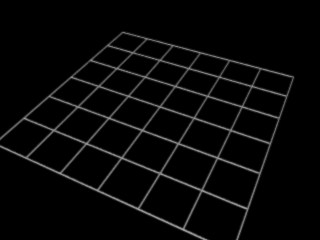
\includegraphics[width=6cm]{pics/grid}
\end{center}
\end{funcdesc}

\section{\module{noise} ---
         Noise functions}

\declaremodule{extension}{cgkit.noise}
\modulesynopsis{A set of basic noise functions}

\begin{funcdesc}{noise}{x[, y[, z[,t]]]}
Returns a noise value (Perlin) in the range from 0 to 1. The arguments
can be up to 4 floating point values or a sequence with up to 4
floating point values (e.g. a \class{vec3} or a \class{vec4}) with an
optional time value. The return value is a pseudo random number in the
range from 0 to 1. Due to the nature of this noise implementation
(gradient noise) the return value at integer lattice points is always 0.5.

As an example, here is a 2D slice (the grid shows the integer lattice):

\begin{center}
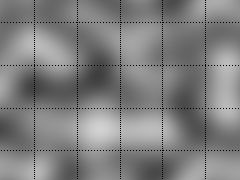
\includegraphics[width=6cm]{pics/noise}
\end{center}

\note{The actual function call depends on the number of arguments, so
calling noise(x,y) is not the same as calling noise(x,y,0). The former
case is a true 2D noise whereas the latter is 3D. The same difference
exists between 3D and 4D.}
\end{funcdesc}

\begin{funcdesc}{snoise}{x[, y[, z[,t]]]}
Returns a signed noise value (Perlin) in the range from -1 to 1. A
call to \code{snoise(args)} is equivalent to \code{2*noise(args)-1}.
\end{funcdesc}

\begin{funcdesc}{pnoise}{point[, t], period[, tperiod]}
Periodic noise function. Basically this is the same as
\function{noise()} but with a periodic return value: \function{pnoise(point)} =
\function{pnoise(point+period)}. The time value can be either part of the point
or it can be specified separately. The point and period must always
have the same dimension. The return value is in the range from 0 to 1.
\end{funcdesc}

\begin{funcdesc}{spnoise}{point[, t], period[, tperiod]}
Signed periodic noise function. The return value is in the range from
-1 to 1. A call to \code{spnoise(args)} is equivalent to 
\code{2*pnoise(args)-1}.
\end{funcdesc}

\begin{funcdesc}{cellnoise}{x[, y[, z[,t]]]}
Returns a pseudo random number which is constant between integer
lattice points. The return value is in the range from 0 to 1.

As an example, here is a 2D slice (the grid shows the integer lattice):

\begin{center}
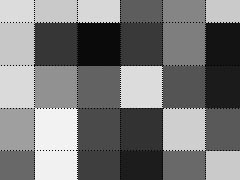
\includegraphics[width=6cm]{pics/cellnoise}
\end{center}
\end{funcdesc}

\begin{funcdesc}{scellnoise}{x[, y[, z[,t]]]}
Signed cell noise. The return value is in the range from -1 to 1. A
call to \code{scellnoise(args)} is equivalent to \code{2*cellnoise(args)-1}.
\end{funcdesc}

\begin{funcdesc}{fBm}{point, octaves, lacunarity=2.0, gain=0.5}
Fractional Brownian motion. The argument point must be a sequence of
either 2 or 3 float values (e.g. a \class{vec3}). This function is a sum of
noise values with different frequencies and amplitudes and is
equivalent to the following code:

\begin{verbatim}
sum = 0.0
amp = 1.0
for i in range(octaves):
    sum += amp*snoise(point)
    amp *= gain
    point *= lacunarity
\end{verbatim}

The return value is in the range from 0 to 1.

As an example, here is a 2D slice (the grid shows the integer lattice):

\begin{center}
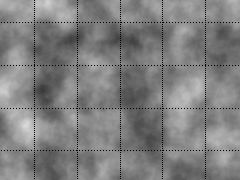
\includegraphics[width=6cm]{pics/fbm}
\end{center}
\end{funcdesc}

\begin{funcdesc}{turbulence}{point, octaves, lacunarity=2.0, gain=0.5}
The code of the turbulence function is very similar to \function{fBm()}. The
difference is that it sums up \code{abs(snoise())} instead of \code{noise()}. 
However, the return value is in the range from 0 to 1.

As an example, here is a 2D slice (the grid shows the integer lattice):

\begin{center}
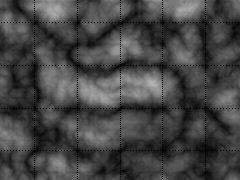
\includegraphics[width=6cm]{pics/turbulence}
\end{center}
\end{funcdesc}


All of the above functions have a vector version that take the same
input parameters but return a vector as result. The output always has
the same dimension than the input. If the time value is specified
separately it does not count to the dimension. For example a call to
\code{vnoise((x,y,z))} returns a \class{vec3}, just as a call to
\code{vnoise((x,y,z),t)}. However, a call to \code{vnoise((x,y,z,t))} 
returns a \class{vec4}.

\begin{funcdesc}{vnoise}{x[, y[, z[,t]]]}
See \function{noise()}.
\end{funcdesc}

\begin{funcdesc}{vsnoise}{x[, y[, z[,t]]]}
See \function{snoise()}.
\end{funcdesc}

\begin{funcdesc}{vpnoise}{point[, t], period[, tperiod]}
See \function{pnoise()}.
\end{funcdesc}

\begin{funcdesc}{vspnoise}{point[, t], period[, tperiod]}
See \function{spnoise()}.
\end{funcdesc}

\begin{funcdesc}{vcellnoise}{x[, y[, z[,t]]]}
See \function{cellnoise()}.
\end{funcdesc}

\begin{funcdesc}{vscellnoise}{x[, y[, z[,t]]]}
See \function{scellnoise()}.
\end{funcdesc}

\begin{funcdesc}{vfBm}{point, octaves, lacunarity=2.0, gain=0.5}
See \function{fBm()}.
\end{funcdesc}

\begin{funcdesc}{vturbulence}{point, octaves, lacunarity=2.0, gain=0.5}
See \function{turbulence()}.
\end{funcdesc}

\section{\module{sl} ---
         RenderMan Shading Language functionality}

\declaremodule{extension}{cgkit.sl}
\modulesynopsis{Provides the same functions than the RenderMan Shading Language}

This module provides some of the functionality from the RenderMan
Shading Language. Those functions that require an actual rendering
context (surfaces, light sources, etc.) are not supported.

Most of the functions can be used just like in the Shading
Language. An exception are those functions whose return type is
dependant on the context as it is the case with \function{random()} or
\function{noise()}. Here, those functions have to be prepended with the 
return type, for example \function{float_random()} or 
\function{point_noise()} (that is, the cast is part of the name).

%----
\subsection{Constants}

\begin{datadesc}{PI}
This is the same as \code{math.pi}.
\end{datadesc}

%-----
\subsection{Math functions}

\begin{funcdesc}{abs}{x}
Returns the absolute value of its argument. This is just the builtin
\function{abs()} function.
\end{funcdesc}

\begin{funcdesc}{acos}{a}
Returns the arc cosine. This function is imported from the
\module{math} module.
\end{funcdesc}

\begin{funcdesc}{asin}{a}
Returns the arc sine. This function is imported from the \module{math} module.
\end{funcdesc}

\begin{funcdesc}{atan}{y[, x]}
Returns the arc tangent. With one argument \function{math.atan()} is
called, with two arguments \function{math.atan2()} is called.
\end{funcdesc}

\begin{funcdesc}{ceil}{x}
Returns the largest integer not greater than \var{x}. This function is
imported from the \module{math} module.
\end{funcdesc}

\begin{funcdesc}{clamp}{x, min, max}
Returns \var{min} if \var{x} < \var{min}, \var{max} if \var{x} > \var{max}, 
otherwise \var{x}.
\end{funcdesc}

\begin{funcdesc}{color_cellnoise}{p}
Returns a color value (actually a \class{vec3}) whose value is a (pseudo)
random function of its arguments. The return value is constant between
integer lattice points.
\end{funcdesc}

\begin{funcdesc}{color_noise}{p}
Returns a color value (actually a \class{vec3}) whose value is a (pseudo)
random function of its arguments.
\end{funcdesc}

\begin{funcdesc}{color_pnoise}{p, period}
Returns a color value (actually a \class{vec3}) whose value is a periodic
(pseudo) random function of its arguments.
\end{funcdesc}

\begin{funcdesc}{color_random}{}
Return a color whose componenets are a random number between 0 and
1. The function actually returns a \class{vec3}.
\end{funcdesc}

\begin{funcdesc}{cos}{a}
Returns the cosine. This function is imported from the \module{math} module.
\end{funcdesc}

\begin{funcdesc}{degrees}{rad}
Converts from radians to degrees.
\end{funcdesc}

\begin{funcdesc}{exp}{x}
Returns \code{pow(e,x)}. This function is imported from the
\module{math} module.
\end{funcdesc}

\begin{funcdesc}{float_cellnoise}{p}
Returns a float value which is a (pseudo) random function of its
arguments. The return value is constant between integer lattice
points. This function is imported from the \module{noise} module.
\end{funcdesc}

\begin{funcdesc}{float_noise}{p}
Returns a float value which is a (pseudo) random function of its
arguments. This function is imported from the \module{noise} module.
\end{funcdesc}

\begin{funcdesc}{float_pnoise}{p, period}
Returns a float value which is a periodic (pseudo) random function of
its arguments. This function is imported from the \module{noise} module.
\end{funcdesc}

\begin{funcdesc}{float_random}{}
Return a random number between 0 and 1. This call is equivalent to
\function{random.random()}.
\end{funcdesc}

\begin{funcdesc}{floor}{x}
Returns the smallest integer not smaller than \var{x}. This function is
imported from the \module{math} module.
\end{funcdesc}

\begin{funcdesc}{inversesqrt}{x}
Returns \code{1/sqrt(x)}.
\end{funcdesc}

\begin{funcdesc}{log}{x[, base]}
Returns the natural logarithm of \var{x} (the same as
\function{math.log}) or the logarithm to the specified base.
\end{funcdesc}

\begin{funcdesc}{max}{a, b, ...}
Returns the argument with maximum value. This is just the builtin
\function{max()} function.
\end{funcdesc}

\begin{funcdesc}{min}{a, b, ...}
Returns the argument with minimum value. This is just the builtin 
\function{min()} function.
\end{funcdesc}

\begin{funcdesc}{mix}{val0, val1, t}
For \var{t}=0 the value \var{val0} is returned, for \var{t}=1 the value 
\var{val1} is returned. For values of \var{t} between 0 and 1 a linearly 
interpolated value is returned.
\end{funcdesc}

\begin{funcdesc}{mod}{a, b}
Returns \code{a\%b}. This is just an equivalent for the \%-operator.
\end{funcdesc}

\begin{funcdesc}{point_cellnoise}{p}
Returns a point (as a \class{vec3}) whose value is a (pseudo) random
function of its arguments. The return value is constant between
integer lattice points.
\end{funcdesc}

\begin{funcdesc}{point_noise}{p}
Returns a point (as a \class{vec3}) whose value is a (pseudo) random function
of its arguments.
\end{funcdesc}

\begin{funcdesc}{point_pnoise}{p, period}
Returns a point (as a \class{vec3}) whose value is a periodic (pseudo) random
function of its arguments.
\end{funcdesc}

\begin{funcdesc}{point_random}{}
Return a point (a \class{vec3}) whose componenets are a random number between
0 and 1.
\end{funcdesc}

\begin{funcdesc}{pow}{x, y}
Returns x**y. This function is imported from the \module{math} module.
\end{funcdesc}

\begin{funcdesc}{radians}{deg}
Converts from degrees to radians.
\end{funcdesc}

\begin{funcdesc}{round}{deg}
Returns the integer closest to \var{x}. This is just the builtin 
\function{round()} function.
\end{funcdesc}

\begin{funcdesc}{sign}{x}
Returns -1 with a negative argument, +1 with a positive argument, and
0 if its argument is zero.
\end{funcdesc}

\begin{funcdesc}{sin}{a}
Returns the sine. This function is imported from the \module{math} module.
\end{funcdesc}

\begin{funcdesc}{smoothstep}{min, max, value}
Returns 0 if \var{value} < \var{min}, 1 if \var{value} > \var{max},
and performs a smooth Hermite interpolation between 0 and 1 in the
interval \var{min} to \var{max}.
\end{funcdesc}

\begin{funcdesc}{spline}{t, controlpoints}
Fits a spline to the control points given and returns the value at \var{t}
which ranges from 0 to 1. At least four control points must always be
given.
\end{funcdesc}

\begin{funcdesc}{sqrt}{x}
Returns the square root. This function is imported from the \module{math}
module.
\end{funcdesc}

\begin{funcdesc}{step}{min, x}
Returns 0 if \var{x} < \var{min}, otherwise 1.
\end{funcdesc}

\begin{funcdesc}{tan}{a}
Returns the tangent. This function is imported from the \module{math} module.
\end{funcdesc}

\begin{funcdesc}{tan}{a}
Returns the tangent. This function is imported from the \module{math} module.
\end{funcdesc}

\begin{funcdesc}{vector_cellnoise}{p}
Returns a vector (as a \class{vec3}) whose value is a (pseudo) random function
of its arguments. The return value is constant between integer lattice
points.
\end{funcdesc}

\begin{funcdesc}{vector_noise}{p}
Returns a vector (as a \class{vec3}) whose value is a (pseudo) random function
of its arguments.
\end{funcdesc}

\begin{funcdesc}{vector_pnoise}{p, period}
Returns a vector (as a \class{vec3}) whose value is a periodic (pseudo) random
function of its arguments.
\end{funcdesc}

%-----
\subsection{Geometric functions}

\begin{funcdesc}{distance}{p1, p2}
Returns the distance between two points. The arguments should be of type 
\class{vec3}.
\end{funcdesc}

\begin{funcdesc}{faceforward}{N, I, Nref}
Flips \var{N} so that it faces in the direction opposite to \var{I}. 

\note{In contrast to the Shading Language \var{Nref} is not optional.}
\end{funcdesc}

\begin{funcdesc}{length}{v}
Returns the length of a vector. This is equivalent to calling 
\method{v.length()}.
\end{funcdesc}

\begin{funcdesc}{normalize}{v}
Returns a unit vector in the direction of \var{v}. This is equivalent to
calling \method{v.normalize()}.
\end{funcdesc}

\begin{funcdesc}{ptlined}{p0, p1, q}
Returns the distance between point \var{q} and the line segment \var{p0},
\var{p1}. The arguments should be of type \class{vec3}.
\end{funcdesc}

\begin{funcdesc}{reflect}{I, N}
Returns the reflection vector given an incident direction \var{I} and a
normal vector \var{N}. This is equivalent to calling \method{I.reflect(N)}.
\end{funcdesc}

\begin{funcdesc}{refract}{I, N, eta}
Returns the transmitted vector given an incident direction \var{I},
the normal vector \var{N} and the relative index of refraction
\var{eta}. This is equivalent to calling \method{I.refract(N, eta)}.
\end{funcdesc}

\begin{funcdesc}{xcomp}{p}
Return the x component of \var{p}. This is equivalent to \code{p.x}.
\end{funcdesc}

\begin{funcdesc}{ycomp}{p}
Return the y component of \var{p}. This is equivalent to \code{p.y}.
\end{funcdesc}

\begin{funcdesc}{zcomp}{p}
Return the z component of \var{p}. This is equivalent to \code{p.z}.
\end{funcdesc}

\begin{funcdesc}{setxcomp}{p, x}
Set the x component of \var{p}. This is equivalent to \code{p.x = x}.
\end{funcdesc}

\begin{funcdesc}{setycomp}{p, y}
Set the y component of \var{p}. This is equivalent to \code{p.y = y}.
\end{funcdesc}

\begin{funcdesc}{setzcomp}{p, z}
Set the z component of \var{p}. This is equivalent to \code{p.z = z}.
\end{funcdesc}

\begin{funcdesc}{comp}{c, index}
Get an individual color component. This is equivalent to \code{c[index]}.
\end{funcdesc}

\begin{funcdesc}{setcomp}{c, index, value}
Set an individual color component. This is equivalent to 
\code{c[index] = value}.
\end{funcdesc}

%-----
\subsection{String functions}

\begin{funcdesc}{concat}{str1, ..., strn}
Returns a concatenated string.
\end{funcdesc}

\begin{funcdesc}{format}{pattern, val1, val2, ..., valn}
Returns a formatted string (similar to the C function
\cfunction{sprintf()}). Any occurance of the character \% followed by a
letter is replaced by a value. In this implementation it doesn't
matter what letter you are actually using (in the Shading Language it
would be \%f for floats, \%p for points, vectors or normals, \%c for
colors, \%m for matrices and \%s for strings).
\end{funcdesc}

\begin{funcdesc}{match}{pattern, subject}
String pattern matching.
\end{funcdesc}

\begin{funcdesc}{printf}{pattern, val1, val2, ..., valn}
Prints the values of the specified variables. Any occurance of the
character \% followed by a letter is replaced by a value. In this
implementation it doesn't matter what letter you are actually using (in
the Shading Language it would be \%f for floats, \%p for points, vectors
or normals, \%c for colors, \%m for matrices and \%s for strings).
\end{funcdesc}

%-----
\subsection{Unsupported functions}

The following functions are not supported by this module:

\begin{itemize}
\item \cfunction{Du()}
\item \cfunction{Dv()}
\item \cfunction{Deriv()}
\item \cfunction{filterstep()}
\end{itemize}

\begin{itemize}
\item \cfunction{area()}
\item \cfunction{calculatenormal()}
\item \cfunction{depth()}
\item \cfunction{fresnel()}
\item \cfunction{transform()}
\item \cfunction{vtransform()}
\item \cfunction{ntransform()}
\end{itemize}

\begin{itemize}
\item \cfunction{ambient()}
\item \cfunction{diffuse()}
\item \cfunction{phong()}
\item \cfunction{specular()}
\item \cfunction{specularbrdf()}
\item \cfunction{trace()}
\end{itemize}

\begin{itemize}
\item \cfunction{environment()}
\item \cfunction{shadow()}
\item \cfunction{texture()}
\item \cfunction{textureinfo()}
\end{itemize}

\begin{itemize}
\item \cfunction{atmosphere()}
\item \cfunction{displacement()}
\item \cfunction{incident()}
\item \cfunction{lightsource()}
\item \cfunction{opposite()}
\item \cfunction{surface()}
\end{itemize}

\begin{itemize}
\item \cfunction{attribute()}
\item \cfunction{option()}
\item \cfunction{rendererinfo()}
\end{itemize}

\section{\module{sltokenize} ---
          Tokenizer for the RenderMan Shading Language}

\declaremodule{extension}{cgkit.sltokenize}
\modulesynopsis{Tokenizer for the RenderMan Shading Language}

This module provides a lexical scanner for the RenderMan Shading
Language. You use it in the same way as the Python tokenize module is
used.

\begin{funcdesc}{tokenize}{readline, tokeneater}
Reads an input stream and creates tokens. The first parameter,
\var{readline}, must be a callable object which provides the same interface
as the \method{readline()} method of built-in file objects. Each call to the
function should return one line of input as a string.

The second parameter, \var{tokeneater}, must also be a callable
object. It is called with six parameters: the token type, the token
string, a tuple (srow, scol) specifying the row and column where the
token begins in the source, a tuple (erow, ecol) giving the ending
position of the token, the line on which the token was found and the
filename of the current file.

The token type can be one of 

\begin{itemize}
\item \code{WHITESPACE}: This is a series of blanks and/or tabs. 
\item \code{NAME}: A valid identifier name or keyword. 
\item \code{NUMBER}: An integer or float. 
\item \code{STRING}: A string enclosed in '"'. 
\item \code{NEWLINE}: A newline character. 
\item \code{OPERATOR}: An operator such as '+', '-', '!', '==', '!=', etc. 
\item \code{CHARACTER}: A single character that doesn't fit anything else. 
\item \code{TYPE}: A Shading Language type (float, point, vector, normal, matrix, color) 
\end{itemize}

By default, the filename argument is an empty string. It will only be
the actual filename if you provide a preprocessed file stream as input
(so you should first run \code{cpp} on any shader). The tokenizer
actually expects preprocessed data as it does not handle comments.
\end{funcdesc}

\section{\module{slparams} ---
          Extracting RenderMan Shader parameters}
\label{slparams}

\declaremodule{extension}{cgkit.slparams}
\modulesynopsis{Extracting RenderMan Shader parameters}

This module can be used to extract the parameters of a RenderMan
shader either from the shader source file or from the compiled shader.
To read parameters from a compiled shader it is necessary that the renderer
package is installed that was used to compile the shader. Currently, the
following renderers are supported:

\begin{itemize}
  \item 3Delight 
  \item Aqsis
  \item Pixie
  \item PRMan
\end{itemize}

Other renderers can be added at runtime (see the \module{sloargs} module).

\begin{funcdesc}{slparams}{slfile, cpp=None, cpperrstream=sys.stderr, includedirs=None, defines=None}
Extracts the shader parameters from a Shading Language source file. 

The argument \var{slfile} is either the name of a compiled shader, the
name of the shader source file (*.sl) or a file-like object that provides the
shader sources.

\var{cpp} determines how the shader source is preprocessed. It can be
either a string containing the name of an external preprocessor tool
(such as \code{cpp}) that must take the file name as parameter and
dump the preprocessed output to stdout. If the preprocessor does not
produce any data a \exception{PreprocessorNotFound} exception is
thrown. The error stream of the preprocessor is written to the object
that is specified by \var{cpperrstream} which must have a
\method{write()} method. If \var{cpperrstream} is \code{None}, the error 
stream is ignored. \var{cpp} can also be a callable object that takes a
filename as input and returns the filtered contents as a string. If
\var{cpp} is \code{None} a simple internal preprocessor based on the 
\module{simplecpp} module is used.

\var{includedirs} is a list of strings that contain directories where to 
look for include files. \var{defines} is a list of tuples (\var{name},
\var{value}) that specify the predefined symbols to use.

The function returns a list of shader info objects. These objects have
four attributes:
    
\begin{itemize}
  \item \var{type}: The type of the shader (\code{"surface"},
  \code{"displacement"}, etc.)
  \item \var{name}: The name of the shader
  \item \var{params}: The shader parameters (see below)
  \item \var{meta}: The shader meta data. How exactly meta data is specified
  depends on the renderer you are using.
\end{itemize}
     
The parameters are given as a list of shader parameter objects describing each
parameter. A shader parameter object has the following attributes:

\begin{itemize}
\item \var{outputSpec}: The output specifier (either \code{"output"} or an empty
string)
\item \var{storage}: The storage class (\code{"uniform"} or \code{"varying"}) 
\item \var{type}: The parameter type 
\item \var{size}: The array length or \code{None} if the parameter is not
an array
\item \var{name}: The name of the parameter 
\item \var{space}: The space in which a point-like type or a color was
defined. If the parameter is an array then this is also an array of space names.
\item \var{default}: The "raw" default value. If the input was a shader source file,
  this will always be a string containing an expression. If the input was
  a compiled shader this will already be an appropriate Python value.
  You should never use this value directly, but always use
  \function{convertdefault()} to obtain a value which can be further processed.
  This way, your code will work for both, compiled shaders and shader source files.
\end{itemize}

For backwards compatibility, the shader info object behaves like a
3-tuple (\var{type}, \var{name}, \var{params}). The meta data can only be
accessed via name though. The shader parameter objects can also be used
like 7-tuples containing the above data (in the order given above).

Example (output slightly reformatted for better readability):
 
\begin{verbatim}
>>> from cgkit import slparams
>>> shaders = lparams.slparams("plastic.sl")
>>> print shaders
[('surface', 'plastic', 
  [('', 'uniform', 'float', None, 'Ka', None, '1'),
   ('', 'uniform', 'float', None, 'Kd', None, '0.5'),
   ('', 'uniform', 'float', None, 'Ks', None, '0.5'),
   ('', 'uniform', 'float', None, 'roughness', None, '0.1'),
   ('', 'uniform', 'color', None, 'specularcolor', 'rgb', '1')])]
>>> shaders[0].type
'surface'
>>> shaders[0].name
'plastic'
>>> for param in shaders[0].params: print param.name
... 
Ka
Kd
Ks
roughness
specularcolor
>>> shaders[0].meta
{}
\end{verbatim}

The parser used inside this function was generated using the parser
generator \ulink{Yapps}{http://theory.stanford.edu/\~{}amitp/Yapps/} 
by Amit Patel.
\end{funcdesc}

\begin{funcdesc}{convertdefault}{paramtuple}
Converts the default value of a shader parameter into a Python
type. The argument \var{paramtuple} must be a 7-tuple (or parameter object) as
returned by \function{slparams()}. The function returns a Python object that corresponds to
the default value of the parameter. If the default value can't be
converted then \code{None} is returned. Only the functions that are
present in the \module{sl} module are evaluated. If a default value
calls a user defined function then \code{None} is returned. The SL
types will be converted into the following Python types:

\begin{tableii}{c|c}{code}{SL type }{ Python type}
\lineii{float}{\code{float}}
\lineii{string}{\code{string}}
\lineii{color}{\code{vec3}}
\lineii{point}{\code{vec3}}
\lineii{vector}{\code{vec3}}
\lineii{normal}{\code{vec3}}
\lineii{matrix}{\code{mat4}}
\end{tableii}

Arrays will be converted into lists of the corresponding type.
\end{funcdesc}

The module defines the following exception classes:

\begin{excdesc}{SLParamsError}
Base class for the exceptions in this module. This class is derived
from the Exception class.
\end{excdesc}

\begin{excdesc}{PreprocessorNotFound}
This exception is thrown when calling the preprocessor didn't produce
any data.
\end{excdesc}

\begin{excdesc}{SyntaxError}
This exception is thrown when a syntax error is found in any function
or shader definition. The exception has the following attributes:

\begin{itemize}
\item \var{filename}: The filename where the error was found 
\item \var{lineno}: The line number where the error was found 
\item \var{line}: The entire line that contains the error 
\item \var{errpos}: The character position where the error token starts
\end{itemize}
\end{excdesc}

\begin{excdesc}{NoMoreTokens}
This exception is thrown when the parser runs out of tokens.
\end{excdesc}

\section{\module{glslangtokenize} ---
          Tokenizer for the OpenGL 2 shading language}

\declaremodule{extension}{cgkit.glslangtokenize}
\modulesynopsis{Tokenizer for the OpenGL 2 shading language}

This module provides a lexical scanner for the OpenGL 2 shading language.
You use it in the same way as the Python tokenize module is used.

\begin{funcdesc}{tokenize}{readline, tokeneater}
Reads an input stream and creates tokens. The first parameter,
\var{readline}, must be a callable object which provides the same interface
as the \method{readline()} method of built-in file objects. Each call to the
function should return one line of input as a string.

The second parameter, \var{tokeneater}, must also be a callable
object. It is called with six parameters: the token type, the token
string, a tuple (srow, scol) specifying the row and column where the
token begins in the source, a tuple (erow, ecol) giving the ending
position of the token, the line on which the token was found and the
filename of the current file.

The token type can be one of 

\begin{itemize}
\item \code{WHITESPACE}: This is a series of blanks and/or tabs. 
\item \code{NAME}: A valid identifier name or keyword. 
\item \code{NUMBER}: An integer or float. 
\item \code{STRING}: A string enclosed in '"'. 
\item \code{NEWLINE}: A newline character. 
\item \code{OPERATOR}: An operator such as '+', '-', '!', '==', '!=', etc. 
\item \code{CHARACTER}: A single character that doesn't fit anything else. 
\item \code{TYPE}: A language type (void, bool, float, int, vec2, vec3, vec4, etc.)
\item \code{QUALIFIER}: A type qualifier (const, attribute, uniform, varying, in, out, inout)
\end{itemize}

By default, the filename argument is an empty string. It will only be
the actual filename if you provide a preprocessed file stream as input
(so you should first run \code{cpp} on any shader). The tokenizer
actually expects preprocessed data as it does not handle comments.
\end{funcdesc}

\section{\module{glslangparams} ---
          Extracting OpenGL 2 shader parameters}
\label{slparams}

\declaremodule{extension}{cgkit.glslangparams}
\modulesynopsis{Extracting OpenGL 2 shader parameters}

This module can be used to extract the parameters of an OpenGL 2 shader
from the shader source file.

\begin{funcdesc}{glslangparams}{shader, cpp=None, cpperrstream=sys.stderr}
Extracts the shader parameters from an OpenGL 2 shader source file.

The argument \var{shader} is either the name of the shader source file or a
file-like object that provides the shader sources. \var{cpp} determines how
the shader source is preprocessed. It can either be a string
containing the name of an external preprocessor tool (such as \code{'cpp'})
that must take the file name as parameter and dump the preprocessed
output to stdout or it can be a callable that takes \var{shader} and
\var{cpperrstream} as input and returns the preprocessed sources as a
string. If the external preprocessor does not produce any data a
\exception{PreprocessorNotFound} exception is thrown.  The error stream of the
preprocessor is written to the object that is specified by
\var{cpperrstream} which must have a write() method. If \var{cpperrstream} is
\code{None}, the error stream is ignored.

If \var{cpp} is None a simple internal preprocessor based on the 
\module{simplecpp} module is used.

The function returns three lists (\var{uniform}, \var{attribute}, 
\var{varying}) that contain the variables with the corresponding qualifier.

A uniform variable is a 5-tuple (\var{type}, \var{identifier}, \var{arraysize},
\var{structname}, \var{struct}). \var{arraysize} is a string containing 
the expression for the length of the array (i.e. the value between the
square brackets). If the variable is no array, \var{arraysize} is
\code{None}.  When the variable is a struct, \var{type} has the value
\code{'struct'}. In this case, the struct is given in \var{struct} (which is
itself a list of variables as 5-tuples). If the struct has a name,
this name is given in \var{structname}, otherwise \var{structname} is 
\code{None}.

An attribute variable is a 2-tuple (\var{type}, \var{identifier}) and a 
varying variable is a 3-tuple (\var{type}, \var{identifier}, \var{arraysize}) 
where \var{arraysize} is defined as in the uniform case.
\end{funcdesc}

The module defines the following exception class:

\begin{excdesc}{GLSLangParseError}
This exception is thrown when an error occurs during parsing the shader
source file.
\end{excdesc}

\section{\module{spacedevice} ---
          Wrapper around the 3Dconnexion Developer's Kits}

\declaremodule{extension}{cgkit.spacedevice}
\modulesynopsis{Wrapper around the 3Dconnexion Developer's Kits}

The \module{spacedevice} module allows applications to support
3D input devices such as a SpaceMouse or a SpaceBall. The module
wraps the 3DxWare SDK by 3Dconnexion. For a more detailed description
of the SDK see the documentation that is part of the
\ulink{SDK}{http://www.3dconnexion.com/sdk.htm}.

The module has to be used in conjunction with a GUI toolkit as there must
be a window that receives the 3D input device events. In principle, any
GUI toolkit can be used as long as it allows obtaining the native windows
handle and accessing system events. The steps necessary to use a 3D input
device are as follows:

\begin{enumerate}
\item Create a \class{SpaceDevice} object.
\item Open the device using the \method{open()} method. This requires a windows
handle of the window that will receive the SpaceDevice events.
\item For every system event received call the \method{translateWin32Event()}
method and check if the event was generated by a SpaceDevice.
If it was, check for the event type and process the event.
\item When the application terminates, call the \method{close()} method to
close the device.

\end{enumerate}

% available()
\begin{funcdesc}{available}{}
Returns \code{True} if the module functionality is available. Currently,
this function will only return \code{True} under Windows and if the
functionality was enabled during compilation.

If this function returns \code{False}, an exception will be raised
whenever you try to instantiate a class from this module.
\end{funcdesc}


\begin{classdesc}{SpaceDevice}{}
The \class{SpaceDevice} class provides the interface to the 3DxWare
library that is used to communicate with the 3D input device. The
constructor of this class calls the SDK function \cfunction{SiInitialize()} 
to initialize the 3DxWare library. The destructor closes the device if
it is open and calls \cfunction{SiTerminate()}.
\end{classdesc}

% open
\begin{methoddesc}{open}{appname, hwnd, devID=SI_ANY_DEVICE}
Establish a connection to a 3D input device. \var{appname} is a string
containing the application name, \var{hwnd} is the native window handle 
(as integer) of the window that should receive the events. \var{devID}
is the device id. An exception is thrown if a connection cannot be
established.

This method calls the SDK functions \cfunction{SiOpenWinInit()} and
\cfunction{SiOpen()}.
\end{methoddesc}

% close
\begin{methoddesc}{close}{}
Close the connection to a device. The function returns immediately if
there is no open connection.

This method calls the SDK function \cfunction{SiClose()}.
\end{methoddesc}

% translateWin32Event
\begin{methoddesc}{translateWin32Event}{msgid, wparam, lparam}
Translates a Win32 event into a SpaceDevice event. The return value is
a tuple (\var{RetVal}, \var{EventType}, \var{Data}).

\var{RetVal} is an object of type
\code{RetVal} that represents an enumeration. It is 
\code{RetVal.IS_EVENT} if the event was generated by a 3D input device,
otherwise it is \code{RetVal.NOT_EVENT}.

\var{EventType} is an object of type \code{EventType} that again represents
an enumeration. It can take one of the following values:

\begin{itemize}
\item \code{EventType.BUTTON_EVENT}
\item \code{EventType.MOTION_EVENT}
\item \code{EventType.ZERO_EVENT}
\item \code{EventType.EXCEPTION_EVENT}
\end{itemize}

The contents of the third value, \var{Data}, depend on the event type:

\begin{tableii}{l|l}{code}{Event type}{Data}
\lineii{BUTTON_EVENT}{(\var{pressed}, \var{released})}
\lineii{MOTION_EVENT}{(\var{translation}, \var{rotation}, \var{period})}
\lineii{ZERO_EVENT}{\code{None}}
\lineii{EXCEPTION_EVENT}{\code{None}}
\end{tableii}

\var{pressed} and \var{released} are each lists that contain the numbers
of the button that were either pressed or released. \var{translation}
is a 3-tuple containing the translation vector and \var{rotation} is a
3-tuple containing the rotation vector. \var{period} contains the time
in milliseconds since the last device event.

This method calls the SDK functions \cfunction{SiGetEventWinInit()} and
\cfunction{SiGetEvent()}.
\end{methoddesc}

% beep
\begin{methoddesc}{beep}{s}
Causes the device to emit a sequence of tones and pauses that is
encoded in the string \var{s}. Lowercase letters represent a tone,
uppercase letters represent a pause.  The closer the letter is to the
beginning of the alphabet the shorter the pause or tone.

This method calls the SDK function \cfunction{SiBeep()}.
\end{methoddesc}

% getDeviceID
\begin{methoddesc}{getDeviceID}{}
Return the device id of the currently open device. 

This method calls the SDK function \cfunction{SiGetDeviceID()}.
\end{methoddesc}

% getDeviceInfo
\begin{methoddesc}{getDeviceInfo}{}
Return information about the currently open device. The return value
is a 5-tuple (\var{device type}, \var{numButtons}, \var{numDegrees},
\var{canBeep}, \var{firmware}). 

This method calls the SDK function \cfunction{SiGetDeviceInfo()}.
\end{methoddesc}

% getDriverInfo
\begin{methoddesc}{getDriverInfo}{}
Return version information about the driver. The return value is a 5-tuple
(\var{major}, \var{minor}, \var{build}, \var{versionstr}, \var{datestr}).

This method calls the SDK function \cfunction{SiGetDriverInfo()}.
\end{methoddesc}

% getNumDevices
\begin{methoddesc}{getNumDevices}{}
Return the number of input devices detected by the driver. 

This method calls the SDK function \cfunction{SiGetNumDevices()}.
\end{methoddesc}

% rezero
\begin{methoddesc}{rezero}{}
Causes the input device's current setting to be defined as the rest
position. 

This method calls the SDK function \cfunction{SiRezero()}.
\end{methoddesc}

% setUIMode
\begin{methoddesc}{setUIMode}{show}
Change the state of the driver menu window from within an application. The
function has to be called before a call to \method{open()}.
\var{show} is a boolean that specifies if the driver menu should be displayed
or not.

This method calls the function \cfunction{SiSetUiMode()}.
\end{methoddesc}


\begin{notice}[note]
The module uses the SDK by 3Dconnexion which can be found at 
\url{http://www.3dconnexion.com/sdk.htm}. The following is the
copyright information of the SDK:

{\em (C) 1998-2001 3Dconnexion 

Permission to use, copy, modify, and distribute this software for all
purposes and without fees is hereby granted provided that this
copyright notice appears in all copies. Permission to modify this
software is granted and 3Dconnexion will support such modifications
only if said modifications are approved by 3Dconnexion}
\end{notice}

% -------------------------------------------------------
\subsection{Example}

Here is a code example that uses pygame (you need at least version 1.7.1)
as GUI toolkit. It simply prints the input device events to the console.

\begin{verbatim}
######################################################################
# SpaceDevice demo
#
# This demo demonstrates the usage of the SpaceDevice object in the
# cgkit.spacedevice module which can be used to access events from
# a SpaceMouse or SpaceBall. You can use this module to add support
# for a SpaceDevice in your own Python application. The demo simply
# prints the events generated from a SpaceDevice to the console.
#
# This demo uses pygame as GUI toolkit (v1.7.1 is required).
# You can use any other GUI toolkit as long as it 1) lets you obtain
# the native window handle of a window and 2) provides access to
# system events.
######################################################################
\end{verbatim}

\begin{verbatim}
import sys
import pygame
from pygame.locals import *
from cgkit import spacedevice
\end{verbatim}

\begin{verbatim}
# handleSystemEvent
def handleSystemEvent(evt):
    """Handle a system event.

    evt is a pygame event object that contains a system event. The function
    first checks if the event was generated by a SpaceDevice and if it was,
    it prints the event data.
    """
    # sdev is the global SpaceDevice object
    global sdev
    
    # Translate the system event into a SpaceDevice event...
    res, evttype, data = sdev.translateWin32Event(evt.msg, evt.wparam, evt.lparam)
    # Check if the event actually was an event generated from
    # the SpaceMouse or SpaceBall...
    print res
    if res!=spacedevice.RetVal.IS_EVENT:
        return

    # Motion event?
    if evttype==spacedevice.EventType.MOTION_EVENT:
        t,r,period = data
        print "Motion: trans:%s rot:%s period:%d"%(t, r, period)
    # Button event?
    elif evttype==spacedevice.EventType.BUTTON_EVENT:
        pressed, released = data
        print "Button: pressed:%s released:%s"%(pressed, released)
    # Zero event?
    elif evttype==spacedevice.EventType.ZERO_EVENT:
        print "Zero"
\end{verbatim}    

\begin{verbatim}
######################################################################

# Check if cgkit was compiled with SpaceDevice support...
if not spacedevice.available():
    print "No SpaceDevice functionality available"
    sys.exit(1)
    
# Initialize pygame...
passed, failed = pygame.init()
if failed>0:
    print "Error initializing pygame"
    sys.exit(1)
\end{verbatim}

\begin{verbatim}
# Open a window...
pygame.display.set_caption("SpaceDevice demo")
srf = pygame.display.set_mode((640,480))

# Enable system events...
pygame.event.set_allowed(SYSWMEVENT)

# Initialize the Space Device...
sdev = spacedevice.SpaceDevice()
info = pygame.display.get_wm_info()
hwnd = info["window"]
sdev.open("Demo", hwnd)
\end{verbatim}

\begin{verbatim}
# Print some information about the driver and the device...
major, minor, build, versionstr, datestr = sdev.getDriverInfo()
print "Driver info:"
print "------------"
print "%s, v%d.%d.%d, %s\n"%(versionstr, major, minor, build, datestr)

devtyp, numbuttons, numdegrees, canbeep, firmware = sdev.getDeviceInfo()
print "Device info:"
print "------------"
print "Device ID:",sdev.getDeviceID()
print "Type     :",devtyp
print "#Buttons :",numbuttons
print "#Degrees :",numdegrees
print "Can beep :",canbeep
print "Firmware :",firmware
print ""
\end{verbatim}

\begin{verbatim}
# Event loop...
running = True
while running:

    # Get a list of events...
    events = pygame.event.get()

    # Process the events...
    for evt in events:

        # Close button?
        if evt.type==QUIT:
            running=False

        # Escape key?
        elif evt.type==KEYDOWN and evt.key==27:
            running=False

        # System event?
        elif evt.type==SYSWMEVENT:
            handleSystemEvent(evt)
\end{verbatim}
            
\begin{verbatim}
# Close the SpaceDevice
sdev.close()
\end{verbatim}
\section{\module{wintab} ---
          Wrapper around the Wintab{\texttrademark} Developer Kit}

\declaremodule{extension}{cgkit.wintab}
\modulesynopsis{Wrapper around the Wintab Developer Kit}

The Wintab{\texttrademark} specification is an open industry standard
interface that provides access to pointing devices such as a pen
tablet, for example. The API was developed by
\ulink{LCS/Telegraphics}{http://www.pointing.com/}.

The \module{wintab} module is a wrapper around the
Wintab{\texttrademark} Developer Kit and can be used to add tablet
support to your Python application. Before you can get any data from
the tablet you have to create an instance of the \class{Context}
class, set the desired parameters and open the context. Once the
context is open you will either receive messages from the tablet
driver or you can poll the current tablet state. Either way, you will
receive the tablet data via \class{Packet} objects that contain all
the data that was generated by the tablet. See also the {\em Wintab
Interface Specification} at \url{http://www.pointing.com/} for more
detailed usage information.

The constants used in this module are either available in the 
\module{wintab} module or in the \module{wintab.constants} module.
The latter can be used if you want to import only the constants into
your namespace.

% available()
\begin{funcdesc}{available}{}
Returns \code{True} if the Wintab functionality is available. As the Wintab
Developer Kit is only available on Windows, this function will always
return \code{False} on other operating systems. 

On Windows, this function can still return \code{False} if either the
Wintab drivers are not installed or cgkit was compiled without Wintab
support.

If this function returns \code{False}, an exception will be raised
whenever you try to call another function or instantiate a class from
this module.
\end{funcdesc}

% info()
\begin{funcdesc}{info}{category}
This function returns a dictionary with global information about the 
interface. \var{category} specifies the category from which information
is being requested. It can be one of the values in the following table:

\begin{tableii}{l|l}{code}{Category}{Description}
\lineii{WTI_INTERFACE}{Global interface identification and capability information}
\lineii{WTI_STATUS}{Current interface resource usage statistics}
\lineii{WTI_DEFCONTEXT}{...}
\lineii{WTI_DEFSYSCTX}{...}
\lineii{WTI_DEVICES+n}{Capability and status information for a device}
\lineii{WTI_CURSORS+n}{Capability and status information for a cursor}
\lineii{WTI_EXTENSIONS+n}{Descriptive information and defaults for an extension}
\lineii{WTI_DDCTXS}{...}
\lineii{WTI_DSCTXS}{...}
\end{tableii}
\end{funcdesc}


\begin{notice}[note]
The module uses the Wintab{\texttrademark} Programmer's Kit which can be
found at \url{http://www.pointing.com/}.

{\em The Wintab Programmer's Kit is copyright 1991-1998 by LCS/Telegraphics.}
\end{notice}

%------------------------------------------------------------------
\subsection{Context class}

The \class{Context} class provides the interface to the tablet driver.

\begin{classdesc}{Context}{}
The class takes no parameters. All the context attributes will be
initialized with the default values as provided by the driver.
\end{classdesc}

Context attributes:

\begin{memberdesc}{name}
Context name.
\end{memberdesc}

\begin{memberdesc}{options}
Specifies options for the context and must be a combination of the following
flags:

\begin{tableii}{l|l}{code}{Option}{Description}
\lineii{CXO_SYSTEM}{The context is a system cursor context}
\lineii{CXO_PEN}{The context is a Pen Windows (and system cursor) context}
\lineii{CXO_MESSAGES}{The context sends WT_PACKET messages to its owner}
\lineii{CXO_MARGIN}{The input context will have a margin}
\lineii{CXO_MGNINSIDE}{The margin will be inside the specified context}
\lineii{CXO_CSRMESSAGES}{The context sends WT_CSRCHANGE messages to its owner}
\end{tableii}
\end{memberdesc}

\begin{memberdesc}{status}
Specifies current status conditions for the context. The status value
is a combination of the following bits:

\begin{tableii}{l|l}{code}{Status bit}{Description}
\lineii{CXS_DISABLED}{The context has been disabled}
\lineii{CXS_OBSCURED}{The context is at least partially obscured by another context}
\lineii{CXS_ONTOP}{The context is the topmost context}
\end{tableii}
\end{memberdesc}

\begin{memberdesc}{locks}
Specifies which attributes of the context the application wishes to be 
locked. The value can be a combination of the following bits:

\begin{tableii}{l|l}{code}{Lock}{Description}
\lineii{CXL_INSIZE}{The input size cannot be changed}
\lineii{CXL_INASPECT}{The input aspect ration cannot be changed}
\lineii{CXL_MARGIN}{The margin options cannot be changed}
\lineii{CXL_SENSITIVITY}{The sensitivity settings for x, y and z cannot be changed}
\lineii{CXL_SYSOUT}{The system pointing control variables cannot be changed}
\end{tableii}
\end{memberdesc}

\begin{memberdesc}{msgbase}
Base number for the message IDs.
\end{memberdesc}

\begin{memberdesc}{device}
Specifies the device whose input the context processes.
\end{memberdesc}

\begin{memberdesc}{pktrate}
Specifies the desired packet report rate in Hertz. Once the context is open,
this field will contain the actual report rate.
\end{memberdesc}

\begin{memberdesc}{pktdata}
Specifies which optional data items will be in packets returned from the
context.
\end{memberdesc}

\begin{memberdesc}{pktmode}
Specifies whether the packet data items will be returned in absolute
or relative mode. If the item's bit is set in this field, the item will
be returned in relative mode.
\end{memberdesc}

\begin{memberdesc}{movemask}
Specifies which packet data items can generate move events in the context.
\end{memberdesc}

\begin{memberdesc}{btndnmask}
Specifies the buttons for which button press events will be processed
in the context.
\end{memberdesc}

\begin{memberdesc}{btnupmask}
Specifies the buttons for which button release events will be processed
in the context.
\end{memberdesc}

\begin{memberdesc}{inorgx}
Specifies the origin of the context's input area in the tablet's
native coordinates along the x axis.
\end{memberdesc}

\begin{memberdesc}{inorgy}
Specifies the origin of the context's input area in the tablet's
native coordinates along the y axis.
\end{memberdesc}

\begin{memberdesc}{inorgz}
Specifies the origin of the context's input area in the tablet's
native coordinates along the z axis.
\end{memberdesc}

\begin{memberdesc}{inextx}
Specifies the extent of the context's input area in the tablet's native
coordinates along the x axis.
\end{memberdesc}

\begin{memberdesc}{inexty}
Specifies the extent of the context's input area in the tablet's native
coordinates along the y axis.
\end{memberdesc}

\begin{memberdesc}{inextz}
Specifies the extent of the context's input area in the tablet's native
coordinates along the z axis.
\end{memberdesc}

\begin{memberdesc}{outorgx}
Specifies the extent of the context's output area in context output
coordinates along the x axis.
\end{memberdesc}

\begin{memberdesc}{outorgy}
Specifies the extent of the context's output area in context output
coordinates along the y axis.
\end{memberdesc}

\begin{memberdesc}{outorgz}
Specifies the extent of the context's output area in context output
coordinates along the z axis.
\end{memberdesc}

\begin{memberdesc}{outextx}
Specifies the extent of the context's output area in context output
coordinates along the x axis.
\end{memberdesc}

\begin{memberdesc}{outexty}
Specifies the extent of the context's output area in context output
coordinates along the y axis.
\end{memberdesc}

\begin{memberdesc}{outextz}
Specifies the extent of the context's output area in context output
coordinates along the z axis.
\end{memberdesc}

\begin{memberdesc}{sensx}
Specifies the relative-mode sensitivity factor for the x axis.
\end{memberdesc}

\begin{memberdesc}{sensy}
Specifies the relative-mode sensitivity factor for the y axis.
\end{memberdesc}

\begin{memberdesc}{sensz}
Specifies the relative-mode sensitivity factor for the z axis.
\end{memberdesc}

\begin{memberdesc}{sysmode}
Specifies the system cursor tracking mode. \code{True} specifies absolute,
\code{False} means relative.
\end{memberdesc}

\begin{memberdesc}{sysorgx}
Specifies the origin in screen coordinates of the screen mapping area
for system cursor tracking.
\end{memberdesc}

\begin{memberdesc}{sysorgy}
Specifies the origin in screen coordinates of the screen mapping area
for system cursor tracking.
\end{memberdesc}

\begin{memberdesc}{sysextx}
Specifies the extent in screen coordinates of the screen mapping area
for system cursor tracking.
\end{memberdesc}

\begin{memberdesc}{sysexty}
Specifies the extent in screen coordinates of the screen mapping area
for system cursor tracking.
\end{memberdesc}

\begin{memberdesc}{syssensx}
Specifies the system-cursor relative-mode sensitivity factor for the
x axis.
\end{memberdesc}

\begin{memberdesc}{syssensy}
Specifies the system-cursor relative-mode sensitivity factor for the
y axis.
\end{memberdesc}

Other attributes:

\begin{memberdesc}{queuesize}
The number of packets the context's queue can hole. Setting this attribute
may result in an exception if the queue size could not be set. In such a
case, you must try again with a smaller value.
\end{memberdesc}

\begin{memberdesc}{id_packet}
The final id of the WT_PACKET message.
\end{memberdesc}

\begin{memberdesc}{id_csrchange}
The final id of the WT_CSRCHANGE message.
\end{memberdesc}

\begin{memberdesc}{id_ctxopen}
The final id of the WT_CTXOPEN message.
\end{memberdesc}

\begin{memberdesc}{id_ctxclose}
The final id of the WT_CTXCLOSE message.
\end{memberdesc}

\begin{memberdesc}{id_ctxupdate}
The final id of the WT_CTXUPDATE message.
\end{memberdesc}

\begin{memberdesc}{id_ctxoverlap}
The final id of the WT_CTXOVERLAP message.
\end{memberdesc}

\begin{memberdesc}{id_proximity}
The final id of the WT_PROXIMITY message.
\end{memberdesc}

\begin{memberdesc}{id_infochange}
The final id of the WT_INFOCHANGE message.
\end{memberdesc}

Methods:

\begin{methoddesc}{open}{hwnd, enable}
Opens the context. \var{hwnd} is the window handle (as integer) of the
window that owns the context and that receives messages from the context.
\var{enable} is a boolean that specifies whether the context will
immediately begin processing input data.

Set the context attributes to the desired values before calling this
method. Modifying context attributes after the context was opened is
possible with the \method{set()} method.
\end{methoddesc}

\begin{methoddesc}{restore}{hwnd, saveinfo, enable}
This method is equivalent to the \method{open()} method with the only
difference that it takes the context attributes via the binary
\var{saveinfo} string which was returned by the \method{save()} method
in a previous session.
\end{methoddesc}

\begin{methoddesc}{close}{}
Closes the context if it was open (or do nothing if it was already closed
or if it was not open at all).
\end{methoddesc}

\begin{methoddesc}{save}{}
Returns a binary \var{saveinfo} string containing the current context state.
This string can be used as argument to the \method{restore()} method.
\end{methoddesc}

\begin{methoddesc}{packet}{serial}
Returns the packet with the specified serial number.
\end{methoddesc}

\begin{methoddesc}{enable}{flag}
If \var{flag} is \code{True} the context is enabled, otherwise it is disabled.
Returns \code{True} if the operation was successful.
\end{methoddesc}

\begin{methoddesc}{overlap}{totop}
If \var{totop} is \code{True} the context will become the topmost context,
otherwise it will be send to the bottom.
Returns \code{True} if the operation was successful.
\end{methoddesc}

\begin{methoddesc}{config}{hwnd=0}
Prompts the user for changes to the context via a dialog box. \var{hwnd}
is the window handle of the window that will be parent of the dialog.
If it is 0, the context owning window will be used.
The return value is \code{True} if the context was changed.
\end{methoddesc}

\begin{methoddesc}{get}{}
Update the local context attributes.
\end{methoddesc}

\begin{methoddesc}{set}{}
Update the tablet context with the settings stored in the local context
attributes.
\end{methoddesc}

\begin{methoddesc}{packetsGet}{maxpkts}
Return the next \var{maxpkts} packets and remove them from the queue.
\end{methoddesc}

\begin{methoddesc}{packetsPeek}{maxpkts}
Return the next \var{maxpkts} packets without removing them from the queue.
\end{methoddesc}

\begin{methoddesc}{dataGet}{begin, end, maxpkts}
Return all packets with serial numbers between \var{begin} and \var{end}
inclusive and remove them from the queue. However, no more than \var{maxpkts}
packets are returned.
The return value is a 2-tuple (\var{numpackets}, \var{packet list}) where
\var{numpackets} is the total number of packets found in the queue between
\var{begin} and \var{end}.
\end{methoddesc}

\begin{methoddesc}{dataPeek}{begin, end, maxpkts}
This is the same as \method{dataGet()} but it doesn't remove the packets
from the queue.
\end{methoddesc}

\begin{methoddesc}{queuePacketsEx}{}
Returns the serial numbers of the oldest and newest packets currently
in the queue.
\end{methoddesc}

%------------------------------------------------------------------
\subsection{Packet class}

\begin{classdesc}{Packet}{}
\end{classdesc}

\begin{memberdesc}{pktdata}
This is a copy of the \code{pktdata} attribute of the corresponding
context, i.e. this attribute determines which of the following attributes
are actually valid.
\end{memberdesc}

\begin{memberdesc}{context}
Specifies the context that generated the event.
\end{memberdesc}

\begin{memberdesc}{status}
Contains a combination of the following status and error conditions:

\begin{tableii}{l|l}{code}{Status bit}{Description}
\lineii{TPS_PROXIMITY}{The cursor is out of the context}
\lineii{TPS_QUEUE_ERR}{The event queue for the context has overflowed}
\lineii{TPS_MARGIN}{The cursor is in the margin of the context}
\lineii{TPS_GRAB}{The cursor is out of the context, but the context has grabbed input}
\lineii{TPS_INVERT}{The cursor is in its inverted state}
\end{tableii}
\end{memberdesc}

\begin{memberdesc}{time}
In absolute mode, specifies the system time at which the event was posted.
In relative mode, specifies the elapsed time in milliseconds since the last
packet.
\end{memberdesc}

\begin{memberdesc}{changed}
Specifies which of the included packet data items have changed since the
previously posted event.
\end{memberdesc}

\begin{memberdesc}{serial}
Contains a serial number assigned to the packet by the context.
\end{memberdesc}

\begin{memberdesc}{cursor}
Specifies which cursor type generated the packet.
\end{memberdesc}

\begin{memberdesc}{buttons}
In absolute, contains the current button state. In relative mode, the low
word contains a button number and the high word contains one of the following
codes: \code{TBN_NONE} if there was no change in button state, \code{TBN_UP}
if the button was released or \code{TBN_DOWN} if the button was pressed.
\end{memberdesc}

\begin{memberdesc}{x}
In absolute mode, contains the scaled cursor location along the x axis.
In relative mode, contains the scaled change in cursor position.
\end{memberdesc}

\begin{memberdesc}{y}
In absolute mode, contains the scaled cursor location along the y axis.
In relative mode, contains the scaled change in cursor position.
\end{memberdesc}

\begin{memberdesc}{z}
In absolute mode, contains the scaled cursor location along the z axis.
In relative mode, contains the scaled change in cursor position.
\end{memberdesc}

\begin{memberdesc}{normalpressure}
In absolute mode, contains the adjusted state of the normal pressure.
In relative mode, contains the change in adjusted pressure state.
\end{memberdesc}

\begin{memberdesc}{tangentpressure}
In absolute mode, contains the adjusted state of the tangential pressure.
In relative mode, contains the change in adjusted pressure state.
\end{memberdesc}

\begin{memberdesc}{orient_azimuth}
Specifies the clockwise rotation of the cursor about the z axis through
a full circular range.
\end{memberdesc}

\begin{memberdesc}{orient_altitude}
Specifies the angle with the x-y plane through a signed, semicircular range.
\end{memberdesc}

\begin{memberdesc}{orient_twist}
Specifies the clockwise rotation of the cursor about its own major axis.
\end{memberdesc}

\begin{memberdesc}{rot_pitch}
Specifies the pitch of the cursor.
\end{memberdesc}

\begin{memberdesc}{rot_roll}
Specifies the roll of the cursor.
\end{memberdesc}

\begin{memberdesc}{rot_yaw}
Specifies the yaw of the cursor.
\end{memberdesc}



\section{\module{glove} ---
          Wrapper around the 5DT Data Glove SDK}

\declaremodule{extension}{cgkit.glove}
\modulesynopsis{Wrapper around the 5DT Data Glove SDK}

This module contains a wrapper around the Data Glove SDK by
\ulink{Fifth Dimension Technologies}{http://www.5dt.com/}. The underlying
SDK can either be version 1 or version 2. Note that some methods are
only implemented if the module was compiled with version 2 of the SDK.
All the functions from the SDK are wrapped as methods of the 
\class{DataGlove} class. Most methods require that a connection to
a glove device was previously established via the \method{open()} method.

% available()
\begin{funcdesc}{available}{}
Returns \code{True} if the Data Glove functionality is available. 

If this function returns \code{False}, an exception will be raised
whenever you try to instantiate a class from this module.
\end{funcdesc}

%------------------------------------------------------------------

\begin{classdesc}{DataGlove}{}
This class encapsulates the data glove handle and contains the
functions from the SDK as methods. Before you can use most of
the methods, you have to establish a connection to a data glove
by calling the \method{open()} method.
\end{classdesc}

% isConnected
\begin{methoddesc}{isConnected}{}
Returns \code{True} if a connection to a data glove was established (i.e.
if \method{open()} was successfully called).
\end{methoddesc}

% open
\begin{methoddesc}{open}{port}
Establish a connection to the data glove at the specified port. \var{port}
is a string containing the serial port to use. For example, under Windows
you might specify \code{"COM1"}, \code{"COM2"}, etc.
\end{methoddesc}

% close
\begin{methoddesc}{close}{}
Disconnect from the glove. The return value is a boolean indicating
if there was an error. Calling \method{close()} while there is no
connection established is not considered an error.
\end{methoddesc}

% getGloveHand
\begin{methoddesc}{getGloveHand}{}
Return the handedness of the glove. The return value is either
\code{FD_HAND_LEFT} or \code{FD_HAND_RIGHT}. If you want a string
representation of the handedness you can use the return value as
key for the dictionary \code{HANDEDNESS}.
\end{methoddesc}

% getGloveType
\begin{methoddesc}{getGloveType}{}
Return the type of the data glove. The return value is one of the following:

\begin{tableii}{l|l}{code}{Type}{Description}
\lineii{FD_GLOVENONE}{No data glove}
\lineii{FD_GLOVE5U}{Data Glove 5 Ultra serial}
\lineii{FD_GLOVE5UW}{Data Glove 5 Ultra serial, wireless}
\lineii{FD_GLOVE5U_USB}{Data Glove 5 Ultra USB}
\lineii{FD_GLOVE7}{Data Glove 5}
\lineii{FD_GLOVE7W}{Data Glove 5, wireless}
\lineii{FD_GLOVE16}{Data Glove 16}
\lineii{FD_GLOVE16W}{Data Glove 16, wireless}
\lineii{FD_GLOVE14U}{Data Glove 14 Ultra serial}
\lineii{FD_GLOVE14UW}{Data Glove 14 Ultra serial, wireless}
\lineii{FD_GLOVE14U_USB}{Data Glove 14 Ultra USB}
\end{tableii}

If you want the string representation of the glove type you can use the
return value as key for the dictionary \code{GLOVETYPE}.

Todo: The above are only the return values of the v2 SDK.
\end{methoddesc}

% getNumSensors
\begin{methoddesc}{getNumSensors}{}
Return the number of sensors.
\end{methoddesc}

% getNumGestures
\begin{methoddesc}{getNumGestures}{}
Return the number of available gestures.
\end{methoddesc}

% getSensorRawAll
\begin{methoddesc}{getSensorRawAll}{}
Return a list with the raw sensor values of all sensors.
\end{methoddesc}

% getSensorRaw
\begin{methoddesc}{getSensorRaw}{sensor}
Return the raw sensor value of the specified sensor. \var{sensor} is an
integer in the range between 0 and \method{getNumSensors()}-1.
\end{methoddesc}

% setSensorRawAll
\begin{methoddesc}{setSensorRawAll}{data}
\end{methoddesc}

\begin{methoddesc}{setSensorRaw}{sensor, raw}
\end{methoddesc}

% getSensorScaledAll
\begin{methoddesc}{getSensorScaledAll}{}
Return a list of the scaled sensor values of all sensors.
\end{methoddesc}

% getSensorScaled
\begin{methoddesc}{getSensorScaled}{sensor}
Return the scaled sensor value of the specified sensor. \var{sensor} is an
integer in the range between 0 and \method{getNumSensors()}-1.
\end{methoddesc}

% getCalibrationAll
\begin{methoddesc}{getCalibrationAll}{}
Return the current auto-calibration settings for all sensors. The return
value is a 2-tuple (\var{lower}, \var{upper}) where \var{lower} is a list
with the minimum values and \var{upper} a list with maximum values.
\end{methoddesc}

% getCalibration
\begin{methoddesc}{getCalibration}{sensor}
Return the auto-calibration for one particular sensor. The return value
is a 2-tuple (\var{lower}, \var{upper}) that contains the minimum and
maximum value.
\end{methoddesc}

% setCalibrationAll
\begin{methoddesc}{setCalibrationAll}{lower, upper}
Set the auto-calibration settings. \var{lower} is a list with the minimum
sensor values and \var{upper} is a list with the maximum values.
\end{methoddesc}

% setCalibration
\begin{methoddesc}{setCalibration}{sensor, lower, upper}
Set the auto-calibration values for one sensor. \var{lower} is the minimum
sensor value and \var{upper} is the maximum value.
\end{methoddesc}

% getSensorMaxAll
\begin{methoddesc}{getSensorMaxAll}{}
Return a list with the maximum scaled values of the sensors.
\end{methoddesc}

% getSensorMax
\begin{methoddesc}{getSensorMax}{sensor}
Return a maximum scaled sensor value for one particular sensor.
\end{methoddesc}

% setSensorMaxAll
\begin{methoddesc}{setSensorMaxAll}{max}
Set the maximum scaled sensor values. \var{max} is a list with the values.
\end{methoddesc}

% setSensorMax
\begin{methoddesc}{setSensorMax}{sensor, max}
Set the maximum scaled sensor value for one sensor.
\end{methoddesc}

% resetCalibration
\begin{methoddesc}{resetCalibration}{[sensor]}
Reset the auto-calibration values. In version 2 of the SDK you can pass
an optional sensor index which will only reset that particular sensor.
\end{methoddesc}

% getGesture
\begin{methoddesc}{getGesture}{}
Return the current gesture.
\end{methoddesc}

% getThresholdAll
\begin{methoddesc}{getThresholdAll}{}
Return the current gesture recognition threshold values. The return
value is a 2-tuple (\var{lower}, \var{upper}) that contains the lower
and upper threshold values.
\end{methoddesc}

% getThreshold
\begin{methoddesc}{getThreshold}{sensor}
Return the gesture recognition threshold values for one sensor. The return
value is a 2-tuple (\var{lower}, \var{upper}) that contains the lower
and upper threshold value.
\end{methoddesc}

% setThresholdAll
\begin{methoddesc}{setThresholdAll}{lower, upper}
Set the gesture recognition threshold values for all sensors. \var{lower}
is a list with the lower threshold values and \var{upper} is a list with
the upper threshold values.
\end{methoddesc}

% setThreshold
\begin{methoddesc}{setThreshold}{sensor, lower, upper}
Set the gesture recognition threshold values for one sensor. \var{lower}
is the lower threshold value and \var{upper} is the upper threshold value.
\end{methoddesc}

% getGloveInfo
\begin{methoddesc}{getGloveInfo}{}
Return a string with glove information.
\end{methoddesc}

% getDriverInfo
\begin{methoddesc}{getDriverInfo}{}
Return a string with driver information.
\end{methoddesc}

% scanUSB
\begin{methoddesc}{scanUSB}{}
Scans the USB for available gloves. The return value is a list with product
IDs of the gloves found. The product IDs can be one of \code{DG14U_R}, 
\code{DG14U_L}, \code{DG5U_R} and \code{DG5U_R}.\\
Availability: {\bf V2}
\end{methoddesc}

% setCallback
\begin{methoddesc}{setCallback}{callback}
Set a callback function that gets called when a new packet was received.
\var{callback} must be a callable object.\\
Availability: {\bf V2}
\end{methoddesc}

% getPacketRate
\begin{methoddesc}{getPacketRate}{}
Return the current packet rate in Hertz.\\
Availability: {\bf V2}
\end{methoddesc}

% newData
\begin{methoddesc}{newData}{}
Returns a boolean that indicates whether new data is available or not.\\
Availability: {\bf V2}
\end{methoddesc}

% getFWVersionMajor
\begin{methoddesc}{getFWVersionMajor}{}
Return the major version of the glove's firmware. This is only implemented
for the Data Glove 14 Ultra. Other gloves will always return 0.\\
Availability: {\bf V2}
\end{methoddesc}

% getFWVersionMinor
\begin{methoddesc}{getFWVersionMinor}{}
Return the minor version of the glove's firmware. This is only implemented
for the Data Glove 14 Ultra. Other gloves will always return 0.\\
Availability: {\bf V2}
\end{methoddesc}

% getAutoCalibrate
\begin{methoddesc}{getAutoCalibrate}{}
Returns \code{True} if auto calibration is activated.\\
Availability: {\bf V2}
\end{methoddesc}

% setAutoCalibrate
\begin{methoddesc}{setAutoCalibrate}{flag}
Enable or disable auto-calibration. If \var{flag} is \code{True} 
auto-calibration is enabled.\\
Availability: {\bf V2}
\end{methoddesc}

% saveCalibration
\begin{methoddesc}{saveCalibration}{filename}
Save the current calibration data to disk.\\
Availability: {\bf V2}
\end{methoddesc}

% loadCalibration
\begin{methoddesc}{loadCalibration}{filename}
Load the calibration settings from a file.\\
Availability: {\bf V2}
\end{methoddesc}



\begin{notice}[note]
The module uses the SDK by Fifth Dimension Technologies (5DT) which
can be found at \url{http://www.5dt.com/}. The following is
the copyright information of the SDK:

{\em Copyright (C) 2000-2004, 5DT <Fifth Dimension Technologies>}
\end{notice}

\section{\module{asfamc} ---
          Acclaim skeleton and motion file (ASF/AMC) reader}

\declaremodule{extension}{cgkit.asfamc}
\modulesynopsis{Acclaim skeleton and motion file (ASF/AMC) reader}

%----------------------------------------------------------------------
\subsection{ASFReader class}

The \class{ASFReader} class reads Acclaim Skeleton Files (ASF) and
calls appropriate methods which have to be implemented in a derived class.

\begin{classdesc}{ASFReader}{filename}
  \var{filename} is the name of the ASF file that should be read.
\end{classdesc}

\begin{methoddesc}{read}{}
Read the entire file.
\end{methoddesc}

\begin{methoddesc}{onVersion}{version}
This method is called when the file format version is encountered.
\var{version} is a float containing the version number.
\end{methoddesc}

\begin{methoddesc}{onName}{name}
This method is called when the skeleton name is read.
\end{methoddesc}

\begin{methoddesc}{onUnits}{units}
This method is called when the units section was read. \var{units}
is a dictionary that contains all definitions that were present in the
units section of the input file. The key is the unit name (such as
\code{mass}, \code{length} and \code{angle}) and the value is the 
corresponding value. If possible the value was cast to float, otherwise
it's still a string.
\end{methoddesc}

\begin{methoddesc}{onDocumentation}{doc}
This method is called when the file documentation was read. \var{doc}
contains the documentation (which may contain several lines).
\end{methoddesc}

\begin{methoddesc}{onRoot}{data}
This method is called when the root section was read. This section contains
information about the root of the skeleton. \var{data} is a dictionary
that contains all the key-value pairs in the root section. The value
is always a tuple (even when it's only one single value). 
\end{methoddesc}

\begin{methoddesc}{onBonedata}{bones}
This method is called after the entire bone data was read. \var{bones}
is a list of bone definitions. Each definition is a data dictionary
containing the key-value pairs in the respective bone section. All values
are tuples (even when it's only one single value). An exception to this
is the \code{limits} attribute which is a list of (\var{min}, \var{max})
tuples that contain the minumum and maximum limits as floats (or as the
special strings \code{"-inf"} and \code{"inf"}).
\end{methoddesc}

\begin{methoddesc}{onHierarchy}{links}
This method is called after the hierarchy section was read. \var{links}
is a list of 2-tuples (\var{parent}, \var{children}) where \var{parent}
is the name of the parent bone and \var{children} is a list of children
bone names.
\end{methoddesc}

%----------------------------------------------------------------------
\subsection{AMCReader class}

The \class{AMCReader} class reads Acclaim Motion Capture Data (AMC) files
and calls \method{onFrame()} for every motion sample in the file.

\begin{classdesc}{AMCReader}{filename}
  \var{filename} is the name of the AMC file that should be read.
\end{classdesc}

\begin{methoddesc}{read}{}
Read the entire file.
\end{methoddesc}

\begin{methoddesc}{onFrame}{framenr, data}
This method is called for every frame. \var{framenr} is the frame number 
and \var{data} is a list of 2-tuples (\var{bone}, \var{values}) where
\var{bone} is a bone name and \var{values} the corresponding 
position/orientation for this frame. The number of values and the
meaning of the values is defined in the corresponding ASF file.
\end{methoddesc}


\section{\module{bvh} ---
        Reading Biovision Hierarchical (BVH) motion capture files}

\declaremodule{extension}{cgkit.bvh}
\modulesynopsis{Reading Biovision Hierarchical (BVH) motion capture files}

This module contains the \class{BVHReader} class which can be used as a base
class for reading Biovision Hierarchical (BVH) files. The class reads the
file and invokes callback methods with the corresponding data in the file.
Derived classes have to implement those callback methods and process
the data as appropriate.

\begin{classdesc}{BVHReader}{filename}
  \var{filename} is the name of the BVH file that should be read.
\end{classdesc}

\begin{methoddesc}{read}{}
Read the entire file.
\end{methoddesc}

\begin{methoddesc}{onHierarchy}{root}
This method is called after the joint hierarchy was read. The entire 
hierarchy is passed in the argument \var{root} which is a \class{Node}
object.
\end{methoddesc}

\begin{methoddesc}{onMotion}{frames, dt}
This method is called when the motion data begins. \var{frames} is the
number of motion samples that follow and \var{dt} is the time interval
that corresponds to one frame.
\end{methoddesc}

\begin{methoddesc}{onFrame}{values}
This method is called for each motion sample (frame) in the
file. \var{values} is a list of floats that contains the position and
angles of the entire skeleton. The order is the same than when
traversing the joint hierarchy in a depth-first manner.
\end{methoddesc}

% ------------------------------------
\subsection{Node objects}

The \method{onHierarchy()} method of the \class{BVHReader} class takes
the joint hierarchy of the skeleton as input. Each node in this hierarchy
is represented by a \class{Node} object that contains all information
stored in the BVH file.

\begin{classdesc*}{Node}
  A \class{Node} object represents one joint in the hierarchy.
\end{classdesc*}

\begin{memberdesc}{name}
This is the name of the joint (or the root).
\end{memberdesc}

\begin{memberdesc}{channels}
This is a list of channel names that are associated with this joint.
This list determines how many values are stored in the motion section
and how they are to be interpreted. Each channel name can be one
of \code{Xposition}, \code{Yposition}, \code{Zposition}, \code{Xrotation},
\code{Yrotation}, \code{Zrotation}.
\end{memberdesc}

\begin{memberdesc}{offset}
This is a 3-tuple of floats containing the offset position of this joint
relative to the parent joint.
\end{memberdesc}

\begin{memberdesc}{children}
This is a list of children joints (which are again described by
\class{Node} objects).
\end{memberdesc}

\begin{methoddesc}{isRoot}{}
Returns \code{True} if the node is the root node.
\end{methoddesc}

\begin{methoddesc}{isEndSite}{}
Returns \code{True} if the node is a leaf.
\end{methoddesc}

\section{\module{objmtl} ---
        Reading Wavefront OBJ/MTL files}

\declaremodule{extension}{cgkit.objmtl}
\modulesynopsis{Reading Wavefront OBJ/MTL files}

This module contains the \class{OBJReader} and \class{MTLReader} classes
which can be used as a base class for reading Wavefront OBJ and MTL files.
The classes read the files and invoke callback methods with the
corresponding data in the file. Derived classes have to implement
those callback methods and process the data as appropriate.

%----------------------------------------------------------------
\subsection{OBJReader class}

The \class{OBJReader} class reads Wavefront OBJ files and calls
appropriate methods which have to be implemented in a derived class.

\begin{classdesc}{OBJReader}{}
  Creates an instance of the reader.
\end{classdesc}

\begin{methoddesc}{read}{f}
Read the content of a file. \var{f} must be a file like object that
can be used to read the content of the file.
\end{methoddesc}

\begin{methoddesc}{begin}{}
Callback method that is called before the file is read.
\end{methoddesc}

\begin{methoddesc}{end}{}
Callback method that is called after the file was read.
\end{methoddesc}

\begin{methoddesc}{handleUnknown}{cmd, arglist}
This method is called when a keyword is encountered that has no 
corresponding handler method.
\end{methoddesc}

The following are the predefined handler methods:

\begin{methoddesc}{call}{filename, *args}
\end{methoddesc}

\begin{methoddesc}{csh}{cmd}
\end{methoddesc}

\begin{methoddesc}{mtllib}{*files}
\end{methoddesc}

\begin{methoddesc}{usemtl}{name}
\end{methoddesc}

\begin{methoddesc}{g}{*groups}
\end{methoddesc}

\begin{methoddesc}{s}{groupnumber}
\end{methoddesc}

\begin{methoddesc}{v}{vert}
\end{methoddesc}

\begin{methoddesc}{vp}{vert}
\end{methoddesc}

\begin{methoddesc}{vn}{normal}
\end{methoddesc}

\begin{methoddesc}{vt}{tvert}
\end{methoddesc}

\begin{methoddesc}{f}{*verts}
\end{methoddesc}

\begin{methoddesc}{o}{name}
\end{methoddesc}

\begin{methoddesc}{bevel}{onoff}
\end{methoddesc}

\begin{methoddesc}{c_interp}{onoff}
\end{methoddesc}

\begin{methoddesc}{d_interp}{onoff}
\end{methoddesc}

\begin{methoddesc}{lod}{level}
\end{methoddesc}

\begin{methoddesc}{shadow_obj}{filename}
\end{methoddesc}

\begin{methoddesc}{trace_obj}{filename}
\end{methoddesc}


%----------------------------------------------------------------
\subsection{MTLReader class}

\begin{methoddesc}{read}{f}
Read the content of a file. \var{f} must be a file like object that
can be used to read the content of the file.
\end{methoddesc}

\begin{methoddesc}{begin}{}
Callback method that is called before the file is read.
\end{methoddesc}

\begin{methoddesc}{end}{}
Callback method that is called after the file was read.
\end{methoddesc}

\begin{methoddesc}{handleUnknown}{cmd, arglist}
This method is called when a keyword is encountered that has no 
corresponding handler method.
\end{methoddesc}

The following are the predefined handler methods:

\begin{methoddesc}{newmtl}{name}
Start of a new material definition.
\end{methoddesc}

\begin{methoddesc}{illum}{model}
Illumination model.
\end{methoddesc}

\begin{methoddesc}{Ka}{col}
Ambient color.
\end{methoddesc}

\begin{methoddesc}{Kd}{col}
Diffuse color.
\end{methoddesc}

\begin{methoddesc}{Ks}{col}
Specular color.
\end{methoddesc}

\begin{methoddesc}{Ke}{col}
Emissive color.
\end{methoddesc}

\begin{methoddesc}{Ns}{shininess}
\end{methoddesc}

\begin{methoddesc}{Ni}{ref}
Refraction index.
\end{methoddesc}

\begin{methoddesc}{Tr}{alpha}
Transparency.
\end{methoddesc}

\begin{methoddesc}{d}{alpha}
Transparency.
\end{methoddesc}

\begin{methoddesc}{Tf}{col}
Transparency.
\end{methoddesc}

\begin{methoddesc}{sharpness}{v}
\end{methoddesc}

\begin{methoddesc}{map_Ka}{mapname, options}
\end{methoddesc}

\begin{methoddesc}{map_Kd}{mapname, options}
\end{methoddesc}

\begin{methoddesc}{map_Ks}{mapname, options}
\end{methoddesc}

\begin{methoddesc}{map_Ke}{mapname, options}
\end{methoddesc}

\begin{methoddesc}{map_Ns}{mapname, options}
\end{methoddesc}

\begin{methoddesc}{map_d}{mapname, options}
\end{methoddesc}

\begin{methoddesc}{map_Bump}{mapname, options}
\end{methoddesc}

\begin{methoddesc}{refl}{mapname, options}
\end{methoddesc}


%----------------------------------------------------------------
\subsection{Handling new keywords}

The \class{OBJReader} and \class{MTLReader} classes can also handle
keywords that are not known to the classes. For each keyword, the
classes look for a method called
\method{handle_<keyword>()} which is invoked with the arguments as
parameters. If such a handler is not found, the \method{handleUnknown()}
method is called.

For the standard keywords such \method{handle_<keyword>()} handlers
are already available. Their task is to preprocess the arguments
and call the final handler method (which is just named after the
keyword).


\section{\module{mayaascii} ---
        Reading Maya ASCII files}

\declaremodule{extension}{cgkit.mayaascii}
\modulesynopsis{Reading Maya ASCII files}

This module contains the \class{MAReader} class which can be used as a
base class for reading Maya ASCII (*.ma) files. The class reads the file
and invokes callback methods with the corresponding data in the
file. Derived classes have to implement those callback methods and
process the data as appropriate.

The module also contains a couple of helper classes that may be
used by a derived reader class to facilitate the processing of the
data.

%----------------------------------------------------------------
\subsection{MAReader class}

The \class{MAReader} class reads Maya ASCII files and calls
appropriate methods which have to be implemented in a derived class.
The content of the file is actually a subset of the {\em Maya Embedded
Language} (MEL) which is the scripting language implemented inside
Maya.  The \class{MAReader} parses the file, breaks down the content
of the file in commands and their arguments and options (expressions
are not evaluated). Each MEL command will then trigger a callback
method that has to execute the command.  These callback methods have
to be implemented in a derived class.

There are 11 MEL commands that can appear in a Maya ASCII 
file\footnote{Actually, there could appear any MEL command, but at least
Maya will only export files containing the above commands.}:

\begin{itemize}
\item {\tt file}
\item {\tt requires}
\item {\tt fileInfo}
\item {\tt currentUnit}
\item {\tt createNode}
\item {\tt setAttr}
\item {\tt addAttr}
\item {\tt connectAttr}
\item {\tt disconnectAttr}
\item {\tt parent}
\item {\tt select}
\end{itemize}

Each command has a number of arguments and can also take options. The
callback methods receive the arguments as regular arguments to the
method and the options as an additional argument \code{opts} which is
a dictionary containing the options that were specified in the
file. The key is the long name of the option (without leading dash)
and the value is a list of strings containing the option values.  The
number of values and how they have to be interpreted depend on the
actual option.

\begin{classdesc}{MAReader}{}
  Creates an instance of the reader.
\end{classdesc}

\begin{methoddesc}{read}{f}
Read the content of a file. \var{f} must be a file like object that
can be used to read the content of the file.
\end{methoddesc}

\begin{methoddesc}{begin}{}
Callback method that is called before the file is read.
\end{methoddesc}

\begin{methoddesc}{end}{}
Callback method that is called after the file was read.
\end{methoddesc}

\begin{methoddesc}{onFile}{filename, opts}
Reference an external file.
\end{methoddesc}

\begin{methoddesc}{onRequires}{product, version}
Specify a requirement that is needed to load the file properly.
\var{product} is a string containing the required software component
and \var{version} is a string containing the required version of that
component.
\end{methoddesc}

\begin{methoddesc}{onFileInfo}{keyword, value, opts}
Specifies information about the file. \var{keyword} and \var{value}
are both strings.
\end{methoddesc}

\begin{methoddesc}{onCurrentUnit}{opts}
Specify the units (linear, angular, time) used in the file.
\end{methoddesc}

\begin{methoddesc}{onCreateNode}{nodetype, opts}
Create a new node. \var{nodetype} is a string specifying the type of node
that is to be created. The new node will automatically be selected (i.e.
subsequent setAttr commands refer to this node).
\end{methoddesc}

\begin{methoddesc}{onSetAttr}{attr, vals, opts}
Set a node attribute. \var{attr} is a string containing the attribute
to be set. \var{vals} is a list of values. The number of elements and
the type of each element depends on the attribute.
\end{methoddesc}

\begin{methoddesc}{onAddAttr}{opts}
Add a new attribute to the node.
\end{methoddesc}

\begin{methoddesc}{onConnectAttr}{srcattr, dstattr, opts}
Connect two attributes. \var{srcattr} is a string specifiying the
attribute that serves as a source and \var{dstattr} is the name of
the attribute that will receive the value. 
\end{methoddesc}

\begin{methoddesc}{onDisconnectAttr}{srcattr, dstattr, opts}
Break the attribute connection between two attributes.
\end{methoddesc}

\begin{methoddesc}{onParent}{objects, parent, opts}
Set the parent of one or more nodes. \var{objects} is a list of node names
and \var{parent} the name of the parent.
\end{methoddesc}

\begin{methoddesc}{onSelect}{objects, opts}
Select a node from a referenced file. \var{objects} is a list of strings
containing the node names.
\end{methoddesc}

%----------------------------------------------------------------
\subsection{Node class}

\begin{classdesc}{Node}{nodetype, opts}
  \var{nodetype} and \var{opts} are the arguments of the 
  \method{onCreateNode()} callback of the \class{MAReader} class.
\end{classdesc}

\begin{methoddesc}{getName}{}
Return the name of the node or \code{None} if no name was specified.
\end{methoddesc}

\begin{methoddesc}{getParentName}{}
Return the name of the parent node or \code{None} if no parent was specified.
\end{methoddesc}

\begin{methoddesc}{setAttr}{attr, vals, opts}
\var{attr}, \var{vals} and \var{opts} are the arguments of the 
\method{onSetAttr()} callback of the \class{MAReader} class. The Python
value of an attribute can be obtained by calling \method{getAttrValue()}.
\end{methoddesc}

\begin{methoddesc}{addAttr}{opts}
\var{opts} is the arguments of the \method{onAddAttr()} callback of 
the \class{MAReader} class.
\end{methoddesc}

\begin{methoddesc}{addInConnection}{localattr, node, attrname}
\end{methoddesc}

\begin{methoddesc}{addOutConnection}{localattr, node, nodename, attrname}
\end{methoddesc}

\begin{methoddesc}{getAttrValue}{lname, sname, type, n=1, default=None}
\end{methoddesc}

\begin{methoddesc}{getInNode}{lname, sname}
\end{methoddesc}

\begin{methoddesc}{getOutAttr}{lname, sname, dstnodetype}
\end{methoddesc}

%----------------------------------------------------------------
\subsection{Attribute class}

The \class{Attribute} class can be used to convert the value of an
attribute (as specified by the \code{setAttr} MEL command) into an
appropriate Python value.

An \class{Attribute} object is initialized with the arguments that
were passed to the \method{onSetAttr()} callback of the reader
class. The value can be retrieved using the \method{getValue()}
method. Whenever you have prior knowledge of the node you are 
currently processing you should pass the expected type of the
attribute to the \method{getValue()} method to prevent the
method from having to guess the type in case it is not specified
in the \code{setAttr} call.

\begin{classdesc}{Attribute}{attr, vals, opts}

\var{attr}, \var{vals} and \var{opts} are the arguments of the 
\method{onSetAttr()} callback of the \class{MAReader} class.

\end{classdesc}

\begin{methoddesc}{getBaseName}{}
Return the base name of the attribute. This is the first part of the
attribute name (and may actually refer to another attribute).

\begin{verbatim}
  ".t"            -> "t"
  ".ed[0:11]"     -> "ed"
  ".uvst[0].uvsn" -> "uvst"
\end{verbatim}
\end{methoddesc}

\begin{methoddesc}{getFullName}{}
Return the full attribute specifier.
\end{methoddesc}

\begin{methoddesc}{getValue}{type=None, n=None}
Return the value of the attribute as an appropriate Python value.
\var{type} is a string containing the required type of the value.
If \code{None} is passed, the method tries to retrieve the value from
the attribute itself. If it fails, an exception is thrown. The following
table lists the valid type strings and their corresponding Python type:

\begin{tableii}{l|l}{code}{type}{Python type}
\lineii{"bool"}{bool}
\lineii{"int"}{int}
\lineii{"float"}{float}
\lineii{"string"}{str}
\lineii{"short2"}{(int, int)}
\lineii{"short3"}{(int, int, int)}
\lineii{"long2"}{(int, int)}
\lineii{"long3"}{(int, int, int)}
\lineii{"int32Array"}{[int, ...]}
\lineii{"float2"}{(float, float)}
\lineii{"float3"}{(float, float, float)}
\lineii{"double2"}{(float, float)}
\lineii{"double3"}{(float, float, float)}
\lineii{"doubleArray"}{[float, ...]}
\lineii{"polyFaces"}{PolyFace (see \ref{polyface})}
\lineii{"nurbsSurface"}{NurbsSurface (see \ref{nurbssurface})}
\lineii{"nurbsCurve"}{NurbsCurve (see \ref{nurbscurve})}
\end{tableii}

The argument \var{n} specifies how many values are expected. An exception
is thrown if the number of values that were set by the \code{setAttr} call
doesn't match the required number. If \code{None} is passed, an arbitrary
number of values is allowed. The value of \var{n} also influences the
return type. If the value is 1 the method will return one of the types
in the above table, otherwise it will return a list of the above types.

\end{methoddesc}

%----------------------------------------------------------------
\subsection{PolyFace class}
\label{polyface}

\begin{classdesc*}{PolyFace}
This class stores the data of a polygonal face. \class{PolyFace} objects
are returned when the value of a \code{polyFaces} attribute is requested.
\end{classdesc*}

The class has the following data members:

\begin{memberdesc}{f}
This is a list of integers containing the edge indices of the edges 
making up the face. If an index is negative the edge has to be
reversed (the edge index then is -i-1).
\end{memberdesc}

\begin{memberdesc}{h}
This is a list of holes. Each hole is described by a list of integers 
containing the edge indices of the edges 
making up the hole in the face. If an index is negative the edge has to be
reversed (the edge index then is -i-1).
\end{memberdesc}

\begin{memberdesc}{mf}
This is a list of texture coordinate ids of the face. This data type
is obsolete as of Maya version 3.0. It is replaced by "mu".
\end{memberdesc}

\begin{memberdesc}{mh}
This is a list of texture coordinate ids of the hole. This data type
is obsolete as of Maya version 3.0. It is replaced by "mu".
\end{memberdesc}

\begin{memberdesc}{mu}
For each loop (i.e. outer loop or hole) this list contains a list of
2-tuples (\var{uvset}, \var{ids}) where \var{uvset} is the index of
the UV set and \var{ids} the indices of the texture coordinates.
\end{memberdesc}

\begin{memberdesc}{fc}
For each loop (outer loop or hole) this list contains a list of color 
index values.
\end{memberdesc}

%----------------------------------------------------------------
\subsection{NurbsSurface class}
\label{nurbssurface}

\begin{classdesc*}{NurbsSurface}
This class stores the data of a NURBS surface. \class{NurbsSurface} objects
are returned when the value of a \code{nurbsSurface} attribute is requested.
\end{classdesc*}

The class has the following data members:

\begin{memberdesc}{udegree}
Degree in u direction.
\end{memberdesc}

\begin{memberdesc}{vdegree}
Degree in v direction.
\end{memberdesc}

\begin{memberdesc}{uform}
Form attribute for the u direction. The attribute can have one of the 
following values:

\begin{tableii}{c|l}{code}{Value}{Meaning}
\lineii{0}{Open}
\lineii{1}{Closed}
\lineii{2}{Periodic}
\end{tableii}
\end{memberdesc}

\begin{memberdesc}{vform}
Form attribute for the v direction (see above).
\end{memberdesc}

\begin{memberdesc}{isrational}
This attribute is \code{True} if the surface contains a rational component.
In this case, the control vertices are given as 4-tuples, otherwise
as 3-tuples. 
\end{memberdesc}

\begin{memberdesc}{uknots}
This is a list of floats containing the knot values for the u direction.
\end{memberdesc}

\begin{memberdesc}{vknots}
This is a list of floats containing the knot values for the v direction.
\end{memberdesc}

\begin{memberdesc}{cvs}
A list of control vertices. Each vertex is given either as a 3-tuple or
4-tuple of floats.
\end{memberdesc}

%----------------------------------------------------------------
\subsection{NurbsCurve class}
\label{nurbscurve}

\begin{classdesc*}{NurbsCurve}
This class stores the data of a NURBS curve. \class{NurbsCurve} objects
are returned when the value of a \code{nurbsCurve} attribute is requested.
\end{classdesc*}

The class has the following data members:

\begin{memberdesc}{degree}
The degree of the curve.
\end{memberdesc}

\begin{memberdesc}{spans}
The number of spans.
\end{memberdesc}

\begin{memberdesc}{form}
Form attribute. The attribute can have one of the following values:

\begin{tableii}{c|l}{code}{Value}{Meaning}
\lineii{0}{Open}
\lineii{1}{Closed}
\lineii{2}{Periodic}
\end{tableii}
\end{memberdesc}

\begin{memberdesc}{isrational}
This attribute is \code{True} if the curve contains a rational component.
In this case, the control vertices have one additional value.
\end{memberdesc}

\begin{memberdesc}{dimension}
The dimension of the curve (2 or 3).
\end{memberdesc}

\begin{memberdesc}{knots}
This is a list of floats containing the knot values.
\end{memberdesc}

\begin{memberdesc}{cvs}
A list of control vertices. Each vertex is a tuple of 2, 3 or 4 floats
(the actual number depends on the \var{dimension} and \var{isrational}
settings).
\end{memberdesc}

\section{\module{lwob} ---
        Reading Lightwave LWOB files}

\declaremodule{extension}{cgkit.lwob}
\modulesynopsis{Reading Lightwave LWOB files}

The documentation for this module will be updated once the module
also handles LWO2 files.

\begin{classdesc}{LWOBReader}{}
  Creates an instance of the reader.
\end{classdesc}


% Hammersley

\section{\module{hammersley} ---
          Generating Hammersley and Halton points}

\declaremodule{extension}{cgkit.hammersley}
\modulesynopsis{Generating Hammersley and Halton points}

This module contains functions to generate points that are uniformly
distributed and stochastic-looking on either a unit square or a unit
sphere. The Hammersley point set is more uniform but is
non-hierarchical, i.e. for different n arguments you get an entirely
new sequence. If you need hierarchical behavior you can use the Halton
point set.

This is a Python version of the implementation provided in:

Tien-Tsin Wong, Wai-Shing Luk, Pheng-Ann Heng\\
{\em Sampling with Hammersley and Halton points}\\
Journal of Graphics Tools, Vol. 2, No. 2, 1997, pp. 9-24\\
\url{http://jgt.akpeters.com/papers/WongLukHeng97/}\\
\url{http://www.cse.cuhk.edu.hk/~ttwong/papers/udpoint/udpoints.html}

% planeHammersley
\begin{funcdesc}{planeHammersley}{n}
Yields a sequence of \var{n} tuples (\var{x}, \var{y}) which represent a
point on the unit square. The sequence of points for a particular \var{n} is
always the same. When \var{n} changes an entirely new sequence will be
generated.
    
This function uses a base of 2.
\end{funcdesc}

% sphereHammersley
\begin{funcdesc}{sphereHammersley}{n}
This function yields \var{n} \class{vec3} objects representing points
on the unit sphere. The sequence of points for a particular \var{n} is
always the same. When \var{n} changes an entirely new sequence will be
generated.

This function uses a base of 2.    
\end{funcdesc}

% planeHalton
\begin{funcdesc}{planeHalton}{n, p2=3}
This function yields a sequence of two floats (\var{x}, \var{y}) which
represent a point on the unit square. The number of points to generate
is given by \var{n}. If \var{n} is set to \code{None}, an infinite
number of points is generated and the caller has to make sure the loop
stops by checking some other critera.  The sequence of generated
points is always the same, no matter what \var{n} is (i.e. the first n
elements generated by the sequence \code{planeHalton(n+1)} is identical to
the sequence \var{planeHalton(n)}).

This function uses 2 as its first prime base whereas the second
prime \var{p2} (which must be a prime number) can be provided by the user.
\end{funcdesc}

% sphereHalton
\begin{funcdesc}{sphereHalton}{n, p2=3}
This function yields a sequence of \class{vec3} objects representing
points on the unit sphere. The number of points to generate is given
by \var{n}. If \var{n} is set to \code{None}, an infinite number of
points is generated and the caller has to make sure the loop stops by
checking some other critera. The sequence of generated points is
always the same, no matter what \var{n} is (i.e. the first n elements
generated by the sequence \code{sphereHalton(n+1)} is identical to the
sequence \code{sphereHalton(n)}).

This function uses 2 as its first prime base whereas the second base
\var{p2} (which must be a prime number) can be provided by the user.
\end{funcdesc}

% ---Copyright---
\begin{notice}[note]
The original C versions of these functions are distributed under the
following license:
  
(c) Copyright 1997, Tien-Tsin Wong\\
ALL RIGHTS RESERVED\\
Permission to use, copy, modify, and distribute this software for
any purpose and without fee is hereby granted, provided that the above
copyright notice appear in all copies and that both the copyright notice
and this permission notice appear in supporting documentation,
 
THE MATERIAL EMBODIED ON THIS SOFTWARE IS PROVIDED TO YOU "AS-IS"
AND WITHOUT WARRANTY OF ANY KIND, EXPRESS, IMPLIED OR OTHERWISE,
INCLUDING WITHOUT LIMITATION, ANY WARRANTY OF MERCHANTABILITY OR
FITNESS FOR A PARTICULAR PURPOSE.  IN NO EVENT SHALL THE AUTHOR
BE LIABLE TO YOU OR ANYONE ELSE FOR ANY DIRECT,
SPECIAL, INCIDENTAL, INDIRECT OR CONSEQUENTIAL DAMAGES OF ANY
KIND, OR ANY DAMAGES WHATSOEVER, INCLUDING WITHOUT LIMITATION,
LOSS OF PROFIT, LOSS OF USE, SAVINGS OR REVENUE, OR THE CLAIMS OF
THIRD PARTIES, WHETHER OR NOT THE AUTHOR HAS BEEN
ADVISED OF THE POSSIBILITY OF SUCH LOSS, HOWEVER CAUSED AND ON
ANY THEORY OF LIABILITY, ARISING OUT OF OR IN CONNECTION WITH THE
POSSESSION, USE OR PERFORMANCE OF THIS SOFTWARE.
\end{notice}

\section{\module{stitch} ---
         Stitching together image tiles}

\declaremodule{extension}{cgkit.stitch}
\modulesynopsis{Stitching together image tiles}

This module can be used to stitch together images that have been
rendered in tiles (using RenderMan's RiCropWindow() functionality, 
for example). If you are using the render tool to create an image
you can use the global value \var{tile} to render the image in tiles
(see section \ref{ribexport}).
The module can also be used as a stand-alone command line utility.

\begin{funcdesc}{stitch}{filename, removetiles=False, infostream=None}
Stitches several image tiles together.   
\var{filename} is the base name of the image that determines the file names
of the tiles. \var{filename} is also the name of the output image.  If
\var{removetiles} is \code{True}, the individual image files will be deleted 
after the image has been stitched. If \var{infostream} is set to a file
like object it is used to output status information about the
stitching process.

The name of an image tile must contain the crop information that was
used to create the image. For example, the name of a tile for an image
"out.tif" could look like this: "out_0.0_0.5_0.75_1.0.tif".  The four
values are the x1,x2,y1,y2 values of the crop window. Those values
together with the resolution of the tile determine the resolution of
the entire image. The position of the tile within that image is given
by x1,y1.
\end{funcdesc}



%---

\chapter{Scene specific modules \label{modules2}}

\localmoduletable

\section{\module{pluginmanager} ---
         Managing plugins}

\declaremodule{extension}{cgkit.pluginmanager}
\modulesynopsis{Managing plugins}

A {\em plugin} is a file that gets imported just like a regular Python
module. Each plugin can be uniquely identified either by its absolute
filename or its module name. The module name is only available once
the plugin is loaded. Any objects (usually classes) that are specially
marked will be made available by the plugin manager for later
retrieval.

A class gets imported if it has an attribute \code{_protocols} which is a
list of supported protocols (a protocol is identified by an arbitrary
hashable object). Each class can be uniquely identified by its module
name and class name.

Plugins are loaded by calling \function{importPlugin()} or 
\function{importPlugins()}. 
You can also register any class as plugin class any time by calling the
\function{register()} function. When a plugin is loaded or an object is
registered the plugin/object is represented by a descriptor class
(\class{PluginDescriptor} resp. \class{PluginObjectDescriptor}). 
These descriptor objects contain information about the plugin/object. The 
object descriptor also holds a reference to the actual plugin object.

You can iterate over all currently available protocols via the
\function{iterProtocols()} function. The \function{iterProtoObjects()} 
function can be used to iterate over all objects that support a
particular protocol and \function{iterObjects()} can be used to
iterate over all objects. The default iterator iterates over all
plugin descriptors.

Example plugin class:

\begin{verbatim}
# file: plugin.py
    
class PluginClass:

    _protocols = ["MyProtocol"]

    def __init__(self):
        ...
    ...
\end{verbatim}

And here's how to use it:

\begin{verbatim}
# Load the plugin
pdesc = importPlugin("plugin.py")
if pdesc.status!=STATUS_OK:
    # there was an error...

# Search a plugin class
objdesc = findObject("plugin.PluginClass")
# Create an instance of the plugin class...
PluginClass = objdesc.object
instance = PluginClass()
\end{verbatim}

The actual functionality is implemented in the \class{PluginManager}
class. However, the module creates a global instance of this class
which can be accessed by the module functions. These functions just
call the corresponding methods of the global plugin manager object.
If you want to load plugins that should be stored separately from
the plugins in your surrounding application then you can also create
your own instance of the \class{PluginManager} class.

% importPlugin
\begin{funcdesc}{importPlugin}{filename, overwrite=False}
Loads a plugin file. The given file is executed, i.e. it is imported
like a module. Any object (usually class or function) that has an
attribute \code{_protocols} is stored in the plugin manager. This
attribute is a list of protocol specifiers (which are just arbitrary
hashable objects).

The file must have a suffix that is recognized as a module by the
Python interpreter (one of the suffixes returned by
\function{imp.get_suffixes()}), otherwise an \exception{UnknownFileType}
exception is thrown.

It is possible to load a plugin several times if \var{overwrite} is set to
\code{True}. The new definitions override the previous ones. However, if
references or instances to old objects are kept somewhere they still
refer to the old definition. When writing a plugin you should always
bear in mind that the file could be executed several times and write
your initialization code accordingly.

The function returns a \class{PluginDescriptor} object which contains
information about the imported plugin.
\end{funcdesc}

% importPlugins
\begin{funcdesc}{importPlugins}{plugins, out=sys.stderr}
Import several plugins at once. \var{plugins} can be a single
file/directory name or a sequence of file/directory names. Directories
are recursively descended.
\var{out} is a stream which is used to output status messages.
\end{funcdesc}

\begin{funcdesc}{register}{obj, name=None, pdesc=None, overwrite=False}
\end{funcdesc}

\begin{funcdesc}{remove}{objdesc}
\end{funcdesc}

\begin{funcdesc}{removePlugin}{pdesc}
\end{funcdesc}

\begin{funcdesc}{removeAll}{}
\end{funcdesc}

\begin{funcdesc}{findPlugin}{filename}
\end{funcdesc}

\begin{funcdesc}{findObject}{name, modname=None}
\end{funcdesc}

\begin{funcdesc}{iterPlugins}{}
\end{funcdesc}

\begin{funcdesc}{iterProtocols}{}
\end{funcdesc}

\begin{funcdesc}{iterProtoObjects}{proto}
\end{funcdesc}

\begin{funcdesc}{iterObjects}{}
\end{funcdesc}

%---------------------------------------------------
\subsection{PluginManager class}

%---------------------------------------------------
\subsection{PluginDescriptor}

A \class{PluginDescriptor} object keeps the status information
of a plugin file. It has the following attributes:

\begin{datadesc}{filename}
The absolute file name of the plugin.
\end{datadesc}

\begin{datadesc}{filedesc}
A file descriptor tuple (\var{suffix}, \var{mode}, \var{type}) as
returned by the \function{get_suffixes()} function in the \module{imp}
module (\var{type} is one of \code{imp.PY_SOURCE}, \code{imp.PY_COMPILED} 
or \code{imp.C_EXTENSION}).
\end{datadesc}

\begin{datadesc}{objcount}
Number of imported objects (usually this should be number of classes + 
number of functions).
\end{datadesc}

\begin{datadesc}{classcount}
Number of imported classes.
\end{datadesc}

\begin{datadesc}{funccount}
Number of imported functions.
\end{datadesc}

\begin{datadesc}{status}
Status flags. If everything is ok the status is \code{STATUS_OK}, otherwise
its a combination of \code{STATUS_EXCEPTION} and \code{STATUS_DUPLICATE}.
\end{datadesc}

\begin{datadesc}{traceback}
A string containing the traceback message (if the \code{STATUS_EXCEPTION}
flag is set).
\end{datadesc}

\begin{datadesc}{objdescs}
A list of object descriptors of all imported objects.
\end{datadesc}

\begin{datadesc}{module}
The module object of the imported plugin.
\end{datadesc}

\begin{datadesc}{modulename}
The name of the plugin module.
\end{datadesc}

%---------------------------------------------------
\subsection{PluginObjectDescriptor}

A \class{PluginObjectDescriptor} object keeps the status information
of a plugin object. It has the following attributes and methods:

\begin{datadesc}{object}
The actual plugin object.
\end{datadesc}

\begin{datadesc}{name}
The name of the object.
\end{datadesc}

\begin{datadesc}{plugindesc}
The \class{PluginDescriptor} of the associated plugin.
\end{datadesc}

\begin{datadesc}{status}
Status flags. If everything is ok the status is \code{STATUS_OK}, otherwise
its \code{STATUS_DUPLICATE}.
\end{datadesc}

\begin{methoddesc}{moduleName}{}
Return the module name where the plugin object belongs to (or None).
\end{methoddesc}

\begin{methoddesc}{objectIdentifier}{}
Return the name under which the object is identified. This name is composed
of the module name and the object name, separated by a dot.
\end{methoddesc}

\section{\module{scene} --- }
\section{\module{eventmanager} ---
         Receiving and routing events}

\declaremodule{extension}{cgkit.eventmanager}
\modulesynopsis{Receiving and routing events}

This module defines the \class{EventManager} class which is used to
manage events. An event is something that occurs at a particular time
and that might trigger actions. Each type of event has to be
identified by a unique name and each occurrence of an event can be 
associated with arbitrary data (for example, if a key press occurs the
data contains the key code).

When dealing with events you have to consider two parts. One part is
producing the events and the other part is consuming them. And it is the 
\class{EventManager} that acts as a broker between the two. Whenever an
event occurs the producer tells the event manager about the event and
the event manager takes care of notifying anyone who showed interest in
this type of event. This way, the producer and consumer don't have to know
each other but can rely on the event manager who is always present (whereas
a particular producer or consumer might not be available all the time).

The event manager distinguishes between system wide events and normal events.
Normal events are those that have a relationship with the current scene
and that are removed if the scene is cleared. On the other hand, system wide
events are independent from the current scene and remain intact if the
scene is cleared.

There is always a global event manager instance that should be used for
managing all events:

\begin{funcdesc}{eventManager}{}
Returns the global event manager object.
\end{funcdesc}


\begin{classdesc}{EventManager}{}
Event manager class. Usually you don't have to create an instance of
this class but use the global event manager instead.
\end{classdesc}

\begin{methoddesc}{event}{name, *params, **keyargs}
Signal the event manager that an event has occurred. The type of event is
identified by the string \var{name} which must be a unique name among all
event types. The remaining arguments are the data associated with this
particular occurrence. This data is passed to the consumers.

The method returns \code{True} if any of the event handlers returned
\code{True} (i.e. the event was consumed). In this case, the notification
chain was interrupted. This means, any event handler that would have been
called after the one that returned \code{True} was not called anymore.
\end{methoddesc}

\begin{methoddesc}{connect}{name, receiver, priority=10, system=False}
Connect a function or method to an event type. Whenever an event of type
\var{name} occurs the event handler specified by \var{receiver} is called.
\var{receiver} can either be a callable such as a function or a method
or it can be an instance of a class that must implement an 
\code{on{\em name}()} method. \var{priority} determines the order in 
which the receivers are invoked. Receivers with lower values (=high priority)
are invoked first.

The argument \var{system} specifies if the connection is system wide or not.
\end{methoddesc}

\begin{methoddesc}{disconnect}{name, receiver=None, system=False}
Disconnect a function or method from the event type \var{name}. The argument
\var{receiver} has the same meaning as in the \method{connect()} method.
If \var{receiver} is \code{None} then all connections from the event
are removed. The argument \var{system} specifies if the connection is
system wide or not.
\end{methoddesc}

\begin{methoddesc}{disconnectAll}{system=False}
Remove all connections from all events. \var{system} specifies whether the
system wide connections or the scene wide connections shall be removed
\end{methoddesc}



\section{\module{events} ---
         Standard event names and classes}

\declaremodule{extension}{cgkit.events}
\modulesynopsis{Standard event names and classes}

This module defines the names of the standard events and the corresponding
event classes.

The actual event name is a capitalized version of the symbol where
all underscores are removed (for example, \code{STEP_FRAME = "StepFrame"}).

\begin{datadesc}{STEP_FRAME}
This event is created whenever the timer is stepped forward one frame
using \code{timer.step()}. The event takes no arguments.
\end{datadesc}

\begin{datadesc}{RESET}
This event is created to reset the simulation/animation. This
effectively sets the time back to 0. Any component that has an
internal state should connect to this method and reset its state
whenever the event is signalled.
\end{datadesc}

\begin{datadesc}{KEY_PRESS}
A key was pressed on the keyboard. The callback function receives 
a \class{KeyEvent} object as argument.
\end{datadesc}

\begin{datadesc}{KEY_RELEASE}
A key was released on the keyboard. The callback function receives 
a \class{KeyEvent} object as argument.
\end{datadesc}

\begin{datadesc}{LEFT_DOWN}
The left mouse button was pressed. The callback function receives 
a \class{MouseButtonEvent} object as argument.
\end{datadesc}

\begin{datadesc}{LEFT_UP}
The left mouse button was released. The callback function receives 
a \class{MouseButtonEvent} object as argument.
\end{datadesc}

\begin{datadesc}{MIDDLE_DOWN}
The middle mouse button was pressed. The callback function receives 
a \class{MouseButtonEvent} object as argument.
\end{datadesc}

\begin{datadesc}{MIDDLE_UP}
The middle mouse button was released. The callback function receives 
a \class{MouseButtonEvent} object as argument.
\end{datadesc}

\begin{datadesc}{RIGHT_DOWN}
The right mouse button was pressed. The callback function receives 
a \class{MouseButtonEvent} object as argument.
\end{datadesc}

\begin{datadesc}{RIGHT_UP}
The right mouse button was released. The callback function receives 
a \class{MouseButtonEvent} object as argument.
\end{datadesc}

\begin{datadesc}{MOUSE_BUTTON_DOWN}
A mouse button other than the left, middle or right button was pressed. The
callback function receives a \class{MouseButtonEvent} object as
argument.
\end{datadesc}

\begin{datadesc}{MOUSE_BUTTON_UP}
A mouse button other than the left, middle or right button was released. The
callback function receives a \class{MouseButtonEvent} object as
argument.
\end{datadesc}

\begin{datadesc}{MOUSE_MOVE}
The mouse was moved. The callback function receives a
\class{MouseMoveEvent} object as argument.
\end{datadesc}

\begin{datadesc}{MOUSE_WHEEL}
The mouse wheel was rotated. The callback function receives a
\class{MouseWheelEvent} object as argument.
\end{datadesc}

\begin{datadesc}{JOYSTICK_AXIS}
\end{datadesc}

\begin{datadesc}{JOYSTICK_BALL}
\end{datadesc}

\begin{datadesc}{JOYSTICK_HAT}
\end{datadesc}

\begin{datadesc}{JOYSTICK_BUTTON_DOWN}
\end{datadesc}

\begin{datadesc}{JOYSTICK_BUTTON_UP}
\end{datadesc}


\begin{datadesc}{SPACE_MOTION}
A SpaceMouse/SpaceBall was moved or rotated. The callback function receives a
\class{SpaceMotionEvent} object as argument.
\end{datadesc}

\begin{datadesc}{SPACE_BUTTON_DOWN}
A SpaceMouse/SpaceBall button was pressed. The callback function receives a
\class{SpaceButtonEvent} object as argument.
\end{datadesc}

\begin{datadesc}{SPACE_BUTTON_UP}
A SpaceMouse/SpaceBall button was released. The callback function receives a
\class{SpaceButtonEvent} object as argument.
\end{datadesc}

\begin{datadesc}{SPACE_BUTTON_ZERO}
The user stopped moving/rotating the SpaceMouse/SpaceBall. The event takes
no arguments.
\end{datadesc}


\begin{datadesc}{TABLET}
A tablet (or similar pointing device) generated an event.
\end{datadesc}


\begin{notice}[note]
It actually depends on the application used to process a scene if a
particular type of event occurs or not. For example, events like a key press
or mouse move do occur in the interactive viewer tool, but not in the
offline rendering tool.
\end{notice}

%-----------
\subsection{KeyEvent object}

The \class{KeyEvent} class is passed as argument to the \code{KEY_PRESS}
and \code{KEY_RELEASE} events. The class contains the attributes
\code{key}, \code{keycode} and \code{mods} (see the constructor for
a description).

\begin{classdesc}{KeyEvent}{key, keycode, mods=0}
\var{key} is a unicode string that contains the key that was 
pressed or released. The key is the translated key which means
that it may depend on other keys (such as Shift) or previously pressed
keys. For example, if you just press the 'a' key you receive a lower
case 'a', but if you press Shift and 'a' then you will get an upper
case 'A'.

\var{keycode} is the code of the untranslated key that was pressed
or released. The values for common keys are defined in the \module{keydefs}
module (i.e. \code{KEY_LEFT}, \code{KEY_UP}, etc.).

\var{mods} contains the modifier flags which is a combination of
\code{KEYMOD_SHIFT}, \code{KEYMOD_CONTROL}, \code{KEYMOD_ALT} and
\code{KEYMOD_META}. The respective flag is set if the Shift, Control,
Alt or Meta key was pressed while the event key was pressed or released.
\end{classdesc}

\begin{methoddesc}{shiftKey}{}
Return \code{True} if the key is a Shift key (no matter if it is the
left or right key).
\end{methoddesc}

\begin{methoddesc}{controlKey}{}
Return \code{True} if the key is a Control key (no matter if it is the
left or right key).
\end{methoddesc}

\begin{methoddesc}{altKey}{}
Return \code{True} if the key is an Alt key (no matter if it is the
left or right key).
\end{methoddesc}

%-----------
\subsection{MouseButtonEvent object}

The \class{MouseButtonEvent} class is passed as argument whenever
a mouse button was pressed or released.

\begin{classdesc}{MouseButtonEvent}{button, x, y, x0, y0}

\var{button} is the mouse button number (1 = left button, 2 = middle button,
3 = right button).

\var{x}/\var{y} is the pixel position of the mouse where 0/0 is the upper
left corner.

\var{x0}/\var{y0} is the normalized position of the mouse where each 
component lies in the range [0,1).

\end{classdesc}

%-----------
\subsection{MouseWheelEvent object}

The \class{MouseWheelEvent} class is passed as argument whenever
the mouse wheel is rotated.

\begin{classdesc}{MouseWheelEvent}{delta, x, y, x0, y0}

\var{delta} is the wheel delta (usually 120 if the wheel was rotated
forward and -120 if the wheel was rotated backward).

\var{x}/\var{y} is the pixel position of the mouse where 0/0 is the upper
left corner.

\var{x0}/\var{y0} is the normalized position of the mouse where each 
component lies in the range [0,1).

\end{classdesc}

%-----------
\subsection{MouseMoveEvent object}

The \class{MouseMoveEvent} class is passed as argument whenever the
mouse is moved.

\begin{classdesc}{MouseMoveEvent}{x, y, dx, dy, x0, y0, dx0, dy0, buttons}

\var{x}/\var{y} is the pixel position of the mouse where 0/0 is the upper
left corner.

\var{dx}/\var{dy} is the mouse delta, i.e. the distance travelled since
the last event.

\var{x0}/\var{y0} is the normalized position of the mouse where each 
component lies in the range [0,1).

\var{dx0}/\var{dy0} is the normalized mouse delta.

\var{buttons} contains the mouse buttons that are currently pressed.
Each bit corresponds to a mouse button (bit 0 = left button, bit 1 = middle
button, etc.).
\end{classdesc}

%-----------
\subsection{JoystickAxisEvent object}

\begin{classdesc}{JoystickAxisEvent}{joystick, axis, value}
\end{classdesc}


\subsection{JoystickHatEvent object}

\begin{classdesc}{JoystickHatEvent}{joystick, hat, x, y}
\end{classdesc}


\subsection{JoystickBallEvent object}

\begin{classdesc}{JoystickBallEvent}{joystick, ball, value}
\end{classdesc}


\subsection{JoystickButtonEvent object}

\begin{classdesc}{JoystickButtonEvent}{joystick, button}
\end{classdesc}

%-----------
\subsection{SpaceMotionEvent object}

\begin{classdesc}{SpaceMotionEvent}{translation, rotation, period}

\var{translation} is a \class{vec3} containing the curreent translation of
the space mouse. The coordinate system of the space mouse is left
handed and such that the X axis points to the right, the Y axis
upwards and the Z axis into the screen.

\var{rotation} is a \class{vec3} containing the current rotation of the
space mouse. The vector is the rotation axis and the magnitude represents
the angle.

\var{period} is the time in milliseconds since the last device event.
\end{classdesc}

\subsection{SpaceButtonEvent object}

\begin{classdesc}{SpaceButtonEvent}{button}
\end{classdesc}

\section{\module{keydefs} ---
         Key code definitions}

\declaremodule{extension}{cgkit.keydefs}
\modulesynopsis{Defines toolkit independent key codes}

This module defines symbolic names for the key codes that are stored
in \class{KeyEvent} objects.

The \code{mods} attribute in the \class{KeyEvent} class is composed
of the following four bits:

\begin{datadesc}{KEYMOD_SHIFT}
Shift bit in the modifier flags.
\end{datadesc}

\begin{datadesc}{KEYMOD_CONTROL}
Control bit in the modifier flags.
\end{datadesc}

\begin{datadesc}{KEYMOD_ALT}
Alt bit in the modifier flags.
\end{datadesc}

\begin{datadesc}{KEYMOD_META}
Meta bit in the modifier flags.
\end{datadesc}


The \code{keycode} attribute in the \class{KeyEvent} class can contain
one of the following values:

\begin{verbatim}
KEY_BACK = 8
KEY_TAB = 9
KEY_RETURN = 13
KEY_ESCAPE = 27
KEY_SPACE = 32

KEY_CAPSLOCK = 2700

KEY_SHIFT_LEFT = 2701
KEY_SHIFT_RIGHT = 2702
KEY_CONTROL_LEFT = 2703
KEY_CONTROL_RIGHT = 2704
KEY_ALT_LEFT = 2705
KEY_ALT_RIGHT = 2706

KEY_PRINT = 2707
KEY_SCROLL = 2708
KEY_PAUSE = 2709

KEY_INSERT = 2710
KEY_DELETE = 127
KEY_HOME = 2712
KEY_END = 2713
KEY_PRIOR = 2714
KEY_NEXT = 2715

KEY_LEFT = 2716
KEY_UP = 2717
KEY_RIGHT = 2718
KEY_DOWN = 2719

KEY_F1 = 2720
KEY_F2 = 2721
KEY_F3 = 2722
KEY_F4 = 2723
KEY_F5 = 2724
KEY_F6 = 2725
KEY_F7 = 2726
KEY_F8 = 2727
KEY_F9 = 2728
KEY_F10 = 2729
KEY_F11 = 2730
KEY_F12 = 2731
KEY_F13 = 2732
KEY_F14 = 2733
KEY_F15 = 2734
KEY_F16 = 2735
KEY_F17 = 2736
KEY_F18 = 2737
KEY_F19 = 2738
KEY_F20 = 2739
KEY_F21 = 2740
KEY_F22 = 2741
KEY_F23 = 2742
KEY_F24 = 2743

KEY_NUMLOCK = 2744

KEY_NUMPAD0 = 2745
KEY_NUMPAD1 = 2746
KEY_NUMPAD2 = 2747
KEY_NUMPAD3 = 2748
KEY_NUMPAD4 = 2749
KEY_NUMPAD5 = 2750
KEY_NUMPAD6 = 2751
KEY_NUMPAD7 = 2752
KEY_NUMPAD8 = 2753
KEY_NUMPAD9 = 2754

KEY_NUMPAD_DECIMAL = 2755
KEY_NUMPAD_ENTER = 2756
KEY_NUMPAD_ADD = 2757
KEY_NUMPAD_SUBTRACT = 2758
KEY_NUMPAD_MULTIPLY = 2759
KEY_NUMPAD_DIVIDE = 2760

KEY_WINDOWS_LEFT = 2761
KEY_WINDOWS_RIGHT = 2762
KEY_WINDOWS_MENU = 2763
\end{verbatim}

\section{\module{preferences} --- }
\section{\module{undo} --- }
\section{\module{slots} ---
         Slot classes}

\declaremodule{extension}{cgkit.slots}
\modulesynopsis{Slot classes}

% -------------------------------------------------
\subsection{Dependent class}

\begin{classdesc}{Dependent}{}
\end{classdesc}

\begin{methoddesc}{onValueChanged}{}
Normal/array
\end{methoddesc}

\begin{methoddesc}{onResize}{newsize}
This method is called by a controlling array slot whenever the size of
the slot has changed.
\end{methoddesc}

\begin{methoddesc}{queryResizeVeto}{size}
Check if a dependent vetoes a resize operation. This method is called
by an array slot on all its dependents whenever the slot size should
be changed to \var{size}. If the
method returns \code{True} the resize operation is rejected. The
default implementation returns \code{False}. Only slots with size
constraints should return \code{True}.
\end{methoddesc}


% -------------------------------------------------
\subsection{Slot classes}

There are the following standard slots:

\begin{itemize}
\item DoubleSlot
\item IntSlot
\item BoolSlot
\item StrSlot
\item PySlot
\item Vec3Slot
\item Vec4Slot
\item Mat3Slot
\item Mat4Slot
\item QuatSlot
\end{itemize}

\begin{classdesc}{Slot}{[value, flags]}
  Create a slot that initially carries the specified value.

  Todo: Describe the flags argument.
\end{classdesc}

%\begin{memberdesc}{_value}
%The current slot value.
%\end{memberdesc}

% isSlotCompatible
\begin{methoddesc}{isSlotCompatible}{slot}
Return \code{True} if \var{slot} is compatible with this slot. Two slots are
compatible if they hold the same type of value. Only compatible slots can be
connected to each other. But note that even when this method returns
true, it can happen that the slots can {\it not} be connected. This is the
case whenever the target just doesn't accept input connections (for
example, because it's computing its output value procedurally).
\end{methoddesc}

% typeName
\begin{methoddesc}{typeName}{}
Return a string containing the name of the stored type. This name can
be used to display the type of the slot to the user. The name should
be chosen so that if two slots cannot be connected to each other then
they should also return different names (however, if two slots have
different names it is still possible that they can be connected to each
other).
\end{methoddesc}

% getController
\begin{methoddesc}{getController}{}
Return the associated controlling slot or \code{None}.
\end{methoddesc}

% setController
\begin{methoddesc}{setController}{slot}
Set or remove a controller for this slot.  The current controller is
replaced with \var{slot} which may also be \code{None} to remove the
current controller only. If the controller is not compatible with this
slot an \exception{EIncompatibleSlotTypes} exception is thrown. 
\end{methoddesc}

% getValue
\begin{methoddesc}{getValue}{}
Return the current slot value.
\end{methoddesc}

% setValue
\begin{methoddesc}{setValue}{val}
Set a new value. If the slot has a controller the new value is
propagated up to the controller. It is then up to the controller how
this new value influences the actual output value. So it is not
guaranteed that the output of the slot is really the new value. When
the value really changes this method triggers the onValueChanged() method
on all dependent objects.
\end{methoddesc}

% connect
\begin{methoddesc}{connect}{slot}
Connect the output of this slot with the input of \var{slot}.
Calling this method is equivalent to calling \code{slot.setController(self)}.
The method has no effect if \var{slot} is \code{None}.
\end{methoddesc}

% disconnect
\begin{methoddesc}{disconnect}{slot}
Breaks an existing connection between this slot and \var{slot}.
Calling this method is equivalent to calling \code{slot.setController(None)}.
The method checks if the connection actually exists before breaking it.
If it does not exist, a \exception{ValueError} exception is raised.
The method has no effect if \var{slot} is \code{None}.
\end{methoddesc}

% addDependent
\begin{methoddesc}{addDependent}{d}
Establish a dependency between this slot and another object \var{d}.
The argument \var{d} is added to the list of dependent objects. This
means that \var{d} somehow depends on the value of this slot and that
\var{d} has to be notified whenever the value of this slot changes.
The actual notification is done by calling \method{notifyDependents()}
which in turn calls \method{onValueChanged()} on all dependent objects.

Todo: C++ warning!
\end{methoddesc}

% removeDependent
\begin{methoddesc}{removeDependent}{d}
Remove the dependency between this slot and another object \var{d}.
\end{methoddesc}

% notifyDependents
\begin{methoddesc}{notifyDependents}{}
Notify all dependent slots about a value change. This method calls the
\method{onValueChanged()} method of all slots whose value depends on the 
value of this slot.
\end{methoddesc}

% computeValue
\begin{methoddesc}{computeValue}{}
This method is used to compute a new value whenever \method{getValue()} is
called and the cache is invalid. It should only be implemented on
procedural slots.
\end{methoddesc}

% -------------------------------------------------
\subsection{ArraySlot classes}

\begin{classdesc}{ArraySlot}{multiplicity=1, constraint=None}
Create an array slot.

\var{multiplicity} is the ``array length'' of one individual item.

\var{constraint} is a SizeConstraint object that constrains the size
of the array slot (see section \ref{sizeconstraints}).
\end{classdesc}

% size
\begin{methoddesc}{size}{}
Return the number of elements in this array slot.
\end{methoddesc}

% isResizable
\begin{methoddesc}{isResizable}{size, ignorelocalconstraint=False}
Check if this slot can currently be resized to a particular size.
This method can be used to check if calling \method{resize()} with
\var{size} as argument would succeed or not.

The method returns \code{False} if either the slot itself is size
constrained or it is connected to a size constrained slot. In the
latter case, the function will return \code{True} again if the
connection is removed. The method will also return \code{True} if
\var{size} matches the constraint size.

If \var{ignorelocalconstraint} is \code{True} the method will
compute its result as if there would no constraint be present in this 
slot (so only dependent objects could reject the resize operation).
\end{methoddesc}

% resize
\begin{methoddesc}{resize}{size}
Resize the array slot so that it can carry \var{size} elements.
The values in the array are not modified by this operation.
\end{methoddesc}

% multiplicity
\begin{methoddesc}{multiplicity}{}
Return the multiplicity of the array slot.
\end{methoddesc}

% copyValues
\begin{methoddesc}{copyValues}{begin, end, target, index}
Copies the slice [\var{begin} : \var{end}] into position \var{index}
of the slot \var{target}. 
If you want to copy one single value you have to pass [n, n+1]. It is also
possible to pass negative values.
For the copy operation to succeed, target has to be of the same type
than this slot.

If any index is out of range, an exception is thrown.

Note: If this method is used to copy values within the same slot then
the target range shouldn't currently overlap with the source slice.
\end{methoddesc}

% isSlotCompatible
\begin{methoddesc}{isSlotCompatible}{slot}
Return \code{True} if \var{slot} is compatible with this slot. Two slots are
compatible if they hold the same type of value. Only compatible slots can be
connected to each other. But note that even when this method returns
true, it can happen that the slots can {\it not} be connected. This is the
case whenever the target just doesn't accept input connections (for
example, because it's computing its output value procedurally).
\end{methoddesc}

% typeName
\begin{methoddesc}{typeName}{}
Return a string containing the name of the stored type. This name can
be used to display the type of the slot to the user. The name should
be chosen so that if two slots cannot be connected to each other then
they should also return different names (however, if two slots have
different names it is still possible that they can be connected to each
other).
\end{methoddesc}

% getController
\begin{methoddesc}{getController}{}
Return the associated controlling slot or \code{None}.
\end{methoddesc}

% setController
\begin{methoddesc}{setController}{slot}
Set or remove a controller for this slot.  The current controller is
replaced with \var{slot} which may also be \code{None} to remove the
current controller only. If the controller is not compatible with this
slot an \exception{EIncompatibleSlotTypes} exception is thrown. 
\end{methoddesc}

% getValue
\begin{methoddesc}{getValue}{index}
Return one item of the array slot. If the multiplicity of the slot is 1
then return value is just an individual value, otherwise it's a tuple
containing the values.
\end{methoddesc}

% setValue
\begin{methoddesc}{setValue}{index, value}
Set one item to a new value. If the multiplicity of the slot is 1 \var{value}
has to be one single value, otherwise it must be a sequence containing
\var{multiplicity} elements.
\end{methoddesc}

% connect
\begin{methoddesc}{connect}{slot}
Connect the output of this slot with the input of \var{slot}.
Calling this method is equivalent to calling \code{slot.setController(self)}.
\end{methoddesc}

% addDependent
\begin{methoddesc}{addDependent}{d}
Establish a dependency between this slot and another object \var{d}.
The argument \var{d} is added to the list of dependent objects. This
means that \var{d} somehow depends on the value of this slot and that
\var{d} has to be notified whenever the value of this slot changes.
The actual notification is done by calling \method{notifyDependents()}
which in turn calls \method{onValueChanged()} on all dependent objects.

Todo: C++ warning!
\end{methoddesc}

% removeDependent
\begin{methoddesc}{removeDependent}{d}
Remove the dependency between this slot and another object \var{d}.
\end{methoddesc}

% notifyDependents
%\begin{methoddesc}{notifyDependents}{}
%Notify all dependent slots about a value change. This method calls the
%\method{onValueChanged()} method of all slots whose value depends on the 
%value of this slot.
%\end{methoddesc}

% -------------------------------------------------
\subsection{SizeConstraint objects}
\label{sizeconstraints}

\class{SizeConstraint} objects can be passed into the constructor of
an array slot to constrain its size. There are two variants, the
\class{LinearSizeConstraint} and the \class{UserSizeConstraint}.
The former constrains an array slot to a size that linearly depends
on the size of another array slot, whereas the latter receives its
size from the user.

% LinearSizeConstraint
\begin{classdesc}{LinearSizeConstraint}{ctrlslot, a=1, b=0}
This class depends its size linearly on the size of another slot.

\var{ctrlslot} is an array slot whose size determines the size of the
constraint.

\var{a} and \var{b} are two coefficients that are used to calculate
the constraint size which is $a \cdot s + b$ where s is the size
of \var{ctrlslot}.
\end{classdesc}

% getCoeffs
\begin{methoddesc}{getCoeffs}{}
Returns a tuple (\var{a}, \var{b}) with the current coefficients.
\end{methoddesc}

% setCoeffs
\begin{methoddesc}{setCoeffs}{a, b}
Set new coefficients for the constraint. The operation might raise an
exception if the new coefficients are not compatible with another
constraint. In this case, the old coefficients remain active.
\end{methoddesc}


% UserSizeConstraint
\begin{classdesc}{UserSizeConstraint}{size=0}
This class stores a size that can be manually set by the user.

\var{size} is the initial size of the constraint.
\end{classdesc}

% setSize
\begin{methoddesc}{setSize}{size}
Set a new constraint size. All slots that are constrained by this object
will be resized. Note that the operation might fail and an exception is
thrown when the resize operation is not allowed (usually because there
are other slots involved that are also size constrained).
\end{methoddesc}


% -------------------------------------------------
\subsection{Procedural slots}

There are the following standard procedural slots:

\begin{itemize}
\item ProceduralDoubleSlot
\item ProceduralIntSlot
\item ProceduralVec3Slot
\item ProceduralVec4Slot
\item ProceduralMat3Slot
\item ProceduralMat4Slot
\item ProceduralQuatSlot
\end{itemize}

% -------------------------------------------------
\subsection{NotificationForwarder class}

A \class{NotificationForwarder} object can be used to forward slot
events from one particular slot to an arbitrary method instead of
the \method{onValueChanged()} or \method{onResize()} method.
To accomplish this the \class{NotificationForwarder} object is
added as a dependent object of the slot. This means, whenever
the value of the slot changes, the \method{onValueChanged()} method
of the \class{NotificationForwarder} object is called which in turn
calls an arbitrary other function or method.

\begin{classdesc}{NotificationForwarder}{onvalchanged, onresize=None}

\var{onvalchanged} is an arbitrary callable object that is invoked whenever a
{\em value changed} event has occured. If the forwarder is used with
a normal slot, the callable does not take any arguments. If it is used
with an array slot, it takes two arguments \var{start} and \var{end} that
specify what range has been modified.

\var{onresize} is a callable that gets called whenever the size of an
array slot has changed. It takes one argument which is the new size of the
slot.
\end{classdesc}

Example:

\begin{verbatim}
>>> from cgkit import *
>>> def myCallback(): print "Something has happened"
...
>>> s=Sphere()
>>> n=NotificationForwarder(myCallback)
>>> s.radius_slot.addDependent(n)
Something has happened
>>> s.radius=5
Something has happened
>>> s.radius=2
Something has happened  
\end{verbatim}


%---
\chapter{Commands \label{commands}}
% cmds

This chapter describes the builtin commands which are implemented in
the \module{cgkit.cmds} module and which are always available. New
commands can be added via the \function{register()} function (for
example, by plugins), so there might actually be more commands
available than are listed here.

% fitCone
\begin{funcdesc}{fitCone}{pos, obj}
Compute a cone that has its apex at \var{pos} and that includes
\var{obj}. The generated cone is the minimal cone that entirely
contains the bounding box of \var{obj} (which must be a
\class{WorldObject}). \var{pos} is the apex of the cone given in world
coordinates. 
The return value is a tuple (\var{n}, \var{w}) where \var{n} is the 
axis direction of the cone and \var{w} is the (full) angle in radians.
\end{funcdesc}

% convertToTriMesh
\begin{funcdesc}{convertToTriMesh}{objs}
Convert all specified objects into triangle meshes. \var{obj} may be an
individual world object or a sequence of objects. Each object may be
specified by name or by reference.
\end{funcdesc}

% setupObjectNames
\begin{funcdesc}{setupObjectNames}{}
Return a string that can be executed to 'import' all scene names.
After executing the returned string you can access all top level
objects via their name.

Example:

\begin{verbatim}
>>> listWorld()
Root
+---Bottom (Box/BoxGeom)
+---GLPointLight (GLPointLight/-)
+---GLPointLight1 (GLPointLight/-)
+---Middle (Sphere/SphereGeom)
+---TargetCamera (TargetCamera/-)
+---Top (Box/BoxGeom)
>>> exec setupObjectNames()
>>> Bottom
<cgkit.box.Box object at 0x094765D0>
>>> TargetCamera
<cgkit.targetcamera.TargetCamera object at 0x09470BD0>
>>> Top
<cgkit.box.Box object at 0x09476690>
\end{verbatim}
\end{funcdesc}

% group()
\begin{funcdesc}{group}{*children, **name}
Group several world objects together. All non keyword arguments
somehow refer to world objects that will all be grouped together. An
argument may be either a \class{WorldObject}, the name of a world
object or a sequence of world objects or names. The name of the new group 
may be given via the \code{name} keyword argument.
The return value is the newly created Group object.

Example:

\begin{verbatim}
>>> b1=Box()
>>> b2=Box()
>>> s1=Sphere()
>>> listWorld()
Root
+---Box (Box/BoxGeom)
+---Box1 (Box/BoxGeom)
+---Sphere (Sphere/SphereGeom)
>>> group("Box", "Box1", s1, name="MyGroup")
>>> listWorld()
Root
+---MyGroup (Group/-)
    +---Box (Box/BoxGeom)
    +---Box1 (Box/BoxGeom)
    +---Sphere (Sphere/SphereGeom)
\end{verbatim}
\end{funcdesc}

% ungroup()
\begin{funcdesc}{ungroup}{group}
Break up a group in its individual components. \var{group} is a group
object or the name of a group object. This function does not only work
with \class{Group} objects but actually with any object that has no direct
geometry assigned to it.

Example:

\begin{verbatim}
>>> listWorld()
Root
+---MyGroup (Group/-)
    +---Box (Box/BoxGeom)
    +---Box1 (Box/BoxGeom)
    +---Sphere (Sphere/SphereGeom)
>>> ungroup("MyGroup")
>>> listWorld()
Root
+---Box (Box/BoxGeom)
+---Box1 (Box/BoxGeom)
+---Sphere (Sphere/SphereGeom)
\end{verbatim}
\end{funcdesc}

% replaceMaterial()
\begin{funcdesc}{replaceMaterial}{name, newmat}
Iterate over all world objects and replace each material called \var{name}
with material object \var{newmat}. 
\end{funcdesc}

% link()
\begin{funcdesc}{link}{childs, parent=None, relative=False}
Link the world objects \var{childs} to \var{parent}. Previously existing
links are removed. If \var{parent} is \code{None} then the links are just
removed. The argument \var{childs} may be either a single world object or
a sequence of world objects. Instead of world objects you can also pass
the names of the world objects.

By default, the absolute position and orientation of the children is
maintained (i.e. the local transform is modified). If you set \var{relative}
to \code{True} the local transform is not modified which will change the
position/orientation of the children (unless the parent transform is the
identity).

Note: The function modifies the name of a child object if there would
be a clash with an existing object under the new parent.
\end{funcdesc}

% drawClear()
\begin{funcdesc}{drawClear}{}
Clear all drawing objects.
\end{funcdesc}

% drawMarker()
\begin{funcdesc}{drawMarker}{pos, col=(1,1,1), size=1}
Draw a marker (a point). \var{col} is the color of the marker and
\var{size} its radius.
\end{funcdesc}

% drawLine()
\begin{funcdesc}{drawLine}{pos1, pos2, col=(1,1,1), size=1}
Draw a line from \var{pos1} to \var{pos2}. \var{col} is the color of the 
line and \var{size} its width.
\end{funcdesc}

% drawText()
\begin{funcdesc}{drawText}{pos, txt, font=None, col=(1,1,1)}
Draw the text \var{txt} at position \var{pos} (3D position). \var{col}
is the color of the text. The text is drawn using GLUT
functionality. \var{font} is a GLUT font constant as defined in the
\module{OpenGL.GLUT} module. It can take one of the following values:

\begin{itemize}
\item \code{GLUT_BITMAP_8_BY_13}
\item \code{GLUT_BITMAP_9_BY_15} (default)
\item \code{GLUT_BITMAP_TIMES_ROMAN_10}
\item \code{GLUT_BITMAP_TIMES_ROMAN_24}
\item \code{GLUT_BITMAP_HELVETICA_10}
\item \code{GLUT_BITMAP_HELVETICA_12}
\item \code{GLUT_BITMAP_HELVETICA_18}
\end{itemize}

\end{funcdesc}

% listWorld()
\begin{funcdesc}{listWorld}{}
List the contents of the world as a tree. Example:

\begin{verbatim}
>>> load("demo4.py")
>>> listWorld()
Root
+---GLDistantLight (GLTargetDistantLight/-)
+---GLDistantLight1 (GLTargetDistantLight/-)
+---Sphere (Sphere/SphereGeom)
|   +---Box0 (Box/BoxGeom)
|   +---Box1 (Box/BoxGeom)
|   +---Box2 (Box/BoxGeom)
|   +---Box3 (Box/BoxGeom)
|   +---Box4 (Box/BoxGeom)
|   +---Box5 (Box/BoxGeom)
|   +---Box6 (Box/BoxGeom)
|   +---Box7 (Box/BoxGeom)
|   +---Box8 (Box/BoxGeom)
|   +---Box9 (Box/BoxGeom)
+---TargetCamera (TargetCamera/-)
\end{verbatim}
\end{funcdesc}

% load()
\begin{funcdesc}{load}{filename, **options}
Loads the given file without deleting the scene, so the contents of
the file is appended to the current scene. Any additional keyword argument
is considered to be an option and is passed to the importer.

To be able to load the file there must be an appropriate import class
(protocol: "Import") available in the plugin manager. The class is
determined by examining the file extension. If no importer is found a
\exception{NoImporter} exception is thrown. See chapter \ref{importplugins}
for the available standard importers.

Any exception generated in the importer is passed to the caller.
\end{funcdesc}

% save()
\begin{funcdesc}{save}{filename, **options}
Saves the current scene. Any additional keyword argument
is considered to be an option and is passed to the exporter.

To be able to save the scene there must be an appropriate export class
(protocol: "Export") available in the plugin manager. The class is
determined by examining the file extension. If no exporter is found a
\exception{NoExporter} exception is thrown. 

Any exception generated in the exporter is passed to the caller.
\end{funcdesc}

% reset()
\begin{funcdesc}{reset}{}
Reset an animation/simulation. This function sets the global time
back to 0 and signals the RESET event.
\end{funcdesc}

% worldObject()
\begin{funcdesc}{worldObject}{obj}
If \var{obj} is a string type this function searches the world object with
that name and returns it. If \var{obj} is not a string, it is returned
unchanged.
\end{funcdesc}

% worldObjects()
\begin{funcdesc}{worldObjects}{objs}
Similar to \function{worldObject()} but the argument may be a sequence of
objects or strings. The return value is always a list, even if only one
object was specified as input.
\end{funcdesc}

% register()
\begin{funcdesc}{register}{cmds,...}
Register functions in the cmds module. The function takes an arbitrary
number of arguments which must be callable objects. Each such function
is registered in the cmds module, so that other modules can call these
functions as if they were implemented directly in the cmds module.
\end{funcdesc}

% importDefaultPlugins
\begin{funcdesc}{importDefaultPlugins}{paths}
Import the default plugins. The plugin files/directories specified by
the \envvar{CGKIT_PLUGIN_PATH} environment variable (if it exists) are
imported.  The function already outputs error messages and returns a
list of plugin descriptors.
\end{funcdesc}

% splitPaths
\begin{funcdesc}{splitPaths}{paths}
Split a string containing paths into the individual paths. The paths
can either be separated by \character{:} or \character{;}. Windows
drive letters are maintained, even when \character{:} is used as separator.

\begin{verbatim}
>>> splitPaths("&:c:\\shaders:c:\\more_shaders;")
['&', 'c:\\shaders', 'c:\\more_shaders']    
\end{verbatim}
\end{funcdesc}

%---
\chapter{The scene\label{scene}}

% Scene class

\section{Scene object}

The \class{Scene} class is a container for anything that should also
be visible to other objects. The "visible" part of the scene is called
the {\em world} which is what gets rendered on screen (everything that
has a coordinate system is part of the world). However, the scene can
also contain objects that are not part of the world. For example, the
global timer or any other object that is used somehow but has no
direct visible representation.

You can retrieve the global scene object by calling the function 
\function{getScene()}. 

\begin{funcdesc}{getScene}{}
Returns the global scene object.
\end{funcdesc}

If a script is invoked via a tool such as the viewer or render tool,
the variable \code{scene} is automatically initialized with the global
scene object. To inspect what objects the scene currently contains,
you can just iterate over a scene:

\begin{verbatim}
>>> for item in scene: print item
...
<cgkit.timer.Timer object at 0x0907FEA0>
<cgkit.worldobject.WorldObject object at 0x0907FE70>
\end{verbatim}

This is what an empty scene looks like. The two scene items you see here
are the globel timer and the root object of the world. These objects are
automatically created by the scene.

%\begin{classdesc}{Scene}{}
%Scene object...
%\end{classdesc}

The scene object has the following attributes and methods:

\begin{memberdesc}{handedness}
Specifies if the scene uses a left-handed or right-handed coordinate
system. The value is a string that is either be \code{'l'} or \code{'r'}.
The default is right handed.
\end{memberdesc}

\begin{memberdesc}{up}
Specifies the direction that is considered to be the "up" direction. The 
value must be a \class{vec3}. The default is (0,0,1) (z axis).
\end{memberdesc}

\begin{memberdesc}{unit}
\end{memberdesc}

\begin{memberdesc}{unit_scale}
\end{memberdesc}

\begin{methoddesc}{worldRoot}{}
Return the root world object.
\end{methoddesc}

\begin{methoddesc}{walkWorld}{root=None}
Walk the world tree and yield each object. This method can be used to
iterator over the entire world tree or a subtree thereof. The argument 
\var{root} specifies the root of the tree which is to traverse (the 
root itself will not be returned).
\end{methoddesc}

\begin{methoddesc}{timer}{}
Return the global timer component (see section \ref{timer}).
\end{methoddesc}

\begin{methoddesc}{clear}{}
Clear the entire scene.
\end{methoddesc}

\begin{methoddesc}{insert}{item}
Insert an item into the scene.
\end{methoddesc}

\begin{methoddesc}{item}{name}
Return the item with the specified name.
\end{methoddesc}

\begin{methoddesc}{worldObject}{name}
Return the world object with the specified name. You can use the character
\character{|} as a path separator.
\end{methoddesc}

\begin{methoddesc}{boundingBox}{}
Return the bounding box of the entire scene.
\end{methoddesc}

\begin{methoddesc}{setJoystick}{joystick}
Set a joystick object.
\end{methoddesc}

\begin{methoddesc}{getJoystick}{id}
Get a joystick object (see section \ref{joystick}). A dummy joystick object is
returned if there is no joystick with the specified id.
\end{methoddesc}

\begin{methoddesc}{hasGlobal}{name}
Return \code{True} if a global option with name \var{name} exists.
\end{methoddesc}

\begin{methoddesc}{getGlobal}{name, default=None}
Get the global option with the given name. \var{default} is returned
if the option does not exist. The options can be set using the 
\class{Globals} class or the \method{setGlobal()} method.
\end{methoddesc}

\begin{methoddesc}{setGlobal}{name, value}
Set the global option \var{name} to \var{value}.
\end{methoddesc}

% Scene globals

\section{Globals}

The \class{Globals} class is a convenience class that just sets the
global attributes in the scene object. You can use it as a shortcut
to set the attributes.

\begin{classdesc}{Globals}{up = (0,0,1), \\
                           handedness = 'r', \\
                           unit = 'm', \\
                           unitscale = 1.0, \\
                           **keyargs}

\var{up} is the global "up" direction.

\var{handedness} specifies whether a left handed or right handed coordinate
system should be used.

\var{unit} and \var{unitscale} specify what 1 unit in 3D space would 
be in the real world.

Any additional argument is stored in the scene as a global option
and can be retrieved using the \method{getGlobal()} method of
the scene object.

\end{classdesc}


%---
\chapter{Components \label{components}}

\declaremodule{}{cgkit}

This chapter lists all available components.

%\localmoduletable

% Component

\section{\class{Component} ---
         Component base class}

A component is just something that has a name to identify it and that
stores slot objects. Usually, the slots are used for providing inputs
to the component which are used to generate outputs that can also be
accessed via slots. The component is then the 'black box' that computes
the output from the input.

\begin{classdesc}{Component}{name = "", \\
		             auto_insert = True}

\var{name} is the name of the component which can be used to identify it.

The component will be inserted into the scene automatically if 
\var{auto_insert} is set to \code{True}.
\end{classdesc}

\begin{memberdesc}{name}
The component's name. You can read and write this attribute.
\end{memberdesc}


% Methods
\begin{methoddesc}{addSlot}{name, slot}
Add a new slot to the component. \var{name} specifies the slot name and
\var{slot} is the slot object. A \exception{KeyError} exception is
thrown if there is already a slot with the specified name.
\end{methoddesc}

\begin{methoddesc}{hasSlot}{name}
Check if a slot with a particular name does exist.
\end{methoddesc}

\begin{methoddesc}{iterSlots}{}
Return an iterator that iterates over all slot names.
\end{methoddesc}

\begin{methoddesc}{numSlots}{}
Return the number of slots in this component.
\end{methoddesc}

\begin{methoddesc}{removeSlot}{name}
Remove the slot with the given name. A \exception{KeyError} exception
is thrown if there is no slot with the specified name.
\end{methoddesc}

\begin{methoddesc}{slot}{name}
Return the slot with the given name. A \exception{KeyError} exception
is thrown if there is no slot with the specified name.
\end{methoddesc}








% Timer component

\section{\class{Timer} ---
         Manages the virtual time}
\label{timer}

The \class{Timer} class manages the virtual time and drives the entire
animation/simulation. Everything that is animated either directly or
indirectly connects to the time slot of the global \class{Timer} instance.
This global timer is automatically created by the scene and can be
obtained by calling the \method{timer()} method of the \class{Scene} class.


\begin{classdesc}{Timer}{name = ''Timer'',\\ 
                         auto_insert = True}


\var{name} is the component name.
\end{classdesc}

% Attributes:

The \class{Timer} class has the following attributes:

\begin{datadesc}{time / time_slot}
Current virtual time in seconds (\code{DoubleSlot}).
This value is increased by \member{timestep} whenever the \method{step()} 
method is called.
\end{datadesc}

\begin{datadesc}{timestep}
The delta time step in seconds that represents one frame.
\end{datadesc}

\begin{datadesc}{duration}
The total duration in seconds of the animation/simulation.
\end{datadesc}

\begin{datadesc}{frame}
Current (fractional) frame number (as float).
\end{datadesc}

\begin{datadesc}{fps}
Current frame rate (as float).
\end{datadesc}

\begin{datadesc}{framecount}
Total number of frames of the animation/simulation (as float).
\end{datadesc}

\begin{datadesc}{clock}
This value contains the value in seconds of the real clock.
\end{datadesc}

% Methods:

The \class{Timer} class has the following methods:

\begin{methoddesc}{startClock}{}
Start the real clock.
\end{methoddesc}

\begin{methoddesc}{stopClock}{}
Stop the real clock.
\end{methoddesc}

\begin{methoddesc}{step}{}
Step to the next frame. This call increases the current virtual time by
\member{timestep} and emits a \code{STEP_FRAME} event.
\end{methoddesc}


% EulerAdapter component

\section{\class{EulerAdapter} ---
         Convert euler angles to mat3, mat4 or quat}

The \class{EulerAdapter} class can be used to convert euler angles
to either a \class{mat3}, a \class{mat4} or a \class{quat}.
For example, you can plug an \class{EulerAdapter} into the position
slot of a world object to specify the orientation of the object via
euler angles.

\begin{classdesc}{EulerAdapter}{anglex = 0,\\ 
                                angley = 0,\\
                                anglez = 0,\\
                                radians = False,\\
                                order = "xyz",\\
                                outtype = "mat3",\\
                                name = "EulerAdapter",\\
                                auto_insert = True}

\var{anglex}, \var{angley} and \var{anglez} are the initial angles around
the x-, y- and z-axis.

\var{radians} determines whether angles are measured in degrees (default)
or radians.

\var{order} is a string with a combination of "x", "y" and "z" and specifies 
the order of the rotations.

\var{outtype} is the type of the output slot and can be one of "mat3",
"mat4" and "quat".
\end{classdesc}

The attributes \var{anglex}, \var{angley} and \var{anglez} always hold
the values of their corresponding slot. The output value is available
as \var{output} / \var{output_slot}.
% Expression component

\section{\class{Expression} ---
         Using expressions to drive animations}

An \class{Expression} outputs a single value that is driven by a user
defined expression. The expression is specified by a string and can
use an arbitrary number of parameters. The parameters and their
default values have to be provided to the constructor via keyword
arguments. An exception is the special variable \code{t} which will always
hold the current time (unless you declare it explicitly).  For each
parameter a slot is created (\code{<name>_slot}), so it is also possible to
animate the parameters. The output value can be accessed via the
\code{output} and \code{output_slot} attributes.

\begin{classdesc}{Expression}{expr = "",\\ 
			      exprtype = None, \\
                              name = "Expression", \\
                              **parameters}

\var{expr} is the expression (in Python syntax) that is used to compute
the output values. It may use mathematical functions defined in the
\module{math} and \module{sl} modules.

\var{exprtype} is the return type of the expression (\code{float}, 
\code{vec3}, ...). If this parameter is not given, the component tries
to figure out the return type itself by evaluating the expression using
the default values and inspecting the return type. If the expression
returns a tuple the output type is automatically set to vec3, vec4, mat3
or mat4 (depending on the number of elements).

\var{name} is the component's name.

Any additional keyword argument is a parameter used in the expression.
Every parameter used in the expression has to be declared except the
variable \code{t} which will automatically receive the current time value.
If you declare \code{t} yourself, it will be just an ordinary variable.
\end{classdesc}


Example:

\begin{verbatim}
s = Sphere()
e = Expression("1.0 + amp*sin(freq*t)", amp=0.2, freq=2.0)
e.output_slot.connect(s.radius_slot)
\end{verbatim}

When the above expression is created, it will have the following slots:

\begin{itemize}
\item \code{output_slot}
\item \code{amp_slot}
\item \code{freq_slot}
\item \code{t_slot}
\end{itemize}
% LookAt component

\section{\class{LookAt} ---
         Align the orientation of objects so they point to a particular target}

The \class{LookAt} component takes a position and target point and 
calculates a rotation matrix that orients an object positioned at the
input position so that the z axis points to target.

The input slots are \var{pos_slot} and \var{target_slot} and the output
slot is \var{output_slot}.

\begin{classdesc}{LookAt}{name = "LookAt",\\ 
			  pos = (0,0,0), \\
                          target = (0,0,0), \\
                          up = (0,0,1), \\
                          roll = 0.0, \\
                          auto_insert = True}

\var{pos} is the position of the object.

\var{target} is the target point that should be aimed at.

\var{up} is the vector that is considered to be the 'up' direction.

\var{roll} is an angle in degrees that the object is rotated around its
local z axis.

\end{classdesc}


% ValueTable component

\section{\class{ValueTable} ---
         Animate a value from a table of values}

A \class{ValueTable} stores time/value pairs and has an output slot that holds
the appropriate value for the current time. The type of the value can
be specified in the constructor. The name of the output slot is always
\var{output_slot}.

\begin{classdesc}{ValueTable}{name = "ValueTable",\\ 
	                      type = "vec3", \\
	                      values = [], \\
	                      modulo = None, \\
	                      tscale = 1.0, \\
                              auto_insert = True}

\var{type} is the type of the values stored in the component. This is also
the type of the output slot.

\var{values} is a list of initial time/value pairs. Each item must
be a 2-tuple (time, value).

\var{modulo} is the duration of the loop. The animation sequence will be
replayed after \var{modulo} seconds. The sequence will not repeat
if \var{modulo} is \code{None}.

\var{tscale} is a scaling factor for the time. Values smaller than 1.0 will
slow down the animation.

\end{classdesc}

\begin{methoddesc}{add}{t, v}
Add a new time/value pair to the table. The value \var{v} must be of
the appropriate type.
\end{methoddesc}


The values can either be added using the \method{add()} method or using
the index operator. If you want to retrieve the value for a particular
time (without using the value slot) then you can either use the call operator
or the index operator:

\begin{verbatim}
>>> vt=ValueTable(type="double")
>>> vt.add(0.0, 1.0)
>>> vt[0.5] = 2.0
>>> list(vt)
[(0.0, 1.0), (0.5, 2.0)]
>>> vt(0.2)
1.0
>>> vt[1.5]
2.0
\end{verbatim}

You can iterate over a \class{ValueTable} to get the time/value pairs:

\begin{verbatim}
>>> vt=ValueTable(type="double")
>>> vt.add(0, 1)
>>> vt.add(1.5, -2)
>>> vt.add(1.0, 0.5)
>>> for t,v in vt: print t,v
...
0 1
1.0 0.5
1.5 -2
\end{verbatim}
% Tunnel component

\section{\class{Tunnel} ---
         Connect slots located on different machines}

A \class{Tunnel} is a component that has an arbitrary number of input slots
and a corresponding output slot for each input slot. The value of the
input slot is simply passed to the output slot. The speciality of the
tunnel is that both ends may reside on two different machines.

%\begin{figure}[htb]
\begin{center}
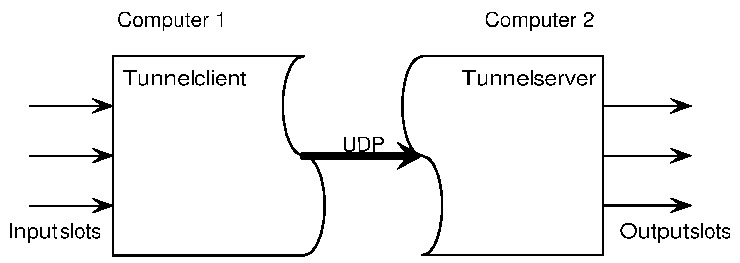
\includegraphics[width=8cm]{pics/tunnel}
%\caption{Tunnel component}
%\label{tunnel_pic}
\end{center}
%\end{figure}

An instance of the tunnel component either represents the input part
(client) or the output part (server). Value changes on the client are
then propagated via UDP datagrams to the server. When creating either
side of the tunnel you have to define the name and type of the slots
that should be created. The slot types of the client and the server
should always match.

\note{ArraySlots are currently not supported.}

\begin{classdesc}{Tunnel}{name = "Tunnel",\\ 
			  server = False, \\
                          slots = None, \\
                          port = 64738, \\
                          host = "localhost", \\
			  gather_messages = False, \\
                          verbose = False, \\
                          auto_insert = True}

\var{server} determines which end of the tunnel is created. The server is
always the ``end'' of a tunnel, i.e. where the values leave the
tunnel.  

\var{slots} specifies the slots to create on the tunnel. It
must be a list of 2-tuples containing two strings. The first string is
the name of the attribute and the second contains the type and
initializer of the slot (in Python syntax). The order and types of the
slots on the client and server should always match.  

\var{port} is the port number to use for the data transfer. The server
listens on this port and the client sends its data to this port on the
target machine.

\var{host} is a string containing the name or IP address of the target
machine where the server part of the tunnel is located. This parameter
is only used on the client side.

\var{gather_messages} determines whether value change messages should be
gathered and sent as one single message or not. If this flag is \code{False},
a message will be sent to the server whenever the value of a slot changes.
However, sometimes it may be the case that you can guarantee that all slots
will change their value at the same time. In such cases, you can set 
\var{gather_messages} to \code{True} which will have the effect that all
messages are collected and delayed until the {\em last} slot receives its 
new value. Only then will the value changes be sent as one big message
which increases the network performance.

If you set \var{verbose} to \code{True} the component will print some
messages so you can follow what it is doing.

\end{classdesc}


Here is an example of a sphere whose position is controlled by a remote
machine:

\begin{verbatim}
# Server code (machine A):

# Create a sphere...
s = Sphere()

# ...and the end of a tunnel that has one Vec3Slot called "pos"
t = Tunnel(
    server = True,
    slots = [("pos", "Vec3Slot()")]
)

# Connect the tunnel slot with the position of the sphere
t.pos_slot.connect(s.pos_slot)
\end{verbatim}

Execute this script with the viewer tool on machine A:

\begin{verbatim}
viewer.py server.py
\end{verbatim}

On the remote machine (the client) you can set the position of the above
sphere with the following code:

\begin{verbatim}
# Client code (machine B):

from cgkit import *

# Create the "entrance" of the tunnel...
t = Tunnel(
    slots = [("pos", "Vec3Slot()")],
    host = "<name or IP of machine A>"
)

# Move the sphere to position (1,0,0)
t.pos_slot.setValue(vec3(1,0,0))
\end{verbatim}

You can call this script by invoking it directly on machine B:

\begin{verbatim}
python client.py
\end{verbatim}

Calling the client code will move the sphere in the first program to 
the position (1,0,0). 

\begin{notice}[note]
As the underlying transport mechanism is using UDP datagrams there is no
error reporting mechanism. The client has no chance of knowing whether
a value change was properly propagated to the server or not. So if you
encounter any problems such as the sphere in the above example {\em not}
moving to another position, you can set the \var{verbose} flag to \code{True}
and additionally check the following points:

\begin{itemize}
\item Do the port numbers on the client and server match?
\item Did you specify the correct host name (or IP address) on the client side?
\item Is there a firewall blocking the network traffic?
\item Did you set \var{gather_messages} to \code{True} and the last slot 
  does not receive any new values? (try to set \var{gather_messages} to
  \code{False})
\end{itemize}

\end{notice}

% ODEDynamics component

\section{\class{ODEDynamics} ---
         Rigid body dynamics using the Open Dynamics Engine}

\begin{classdesc}{ODEDynamics}{name = "ODEDynamics",\\ 
			       gravity = 9.81, \\
                               substeps = 1, \\
                               enabled = True, \\
                               erp = None, \\
                               cfm = None, \\
                               defaultcontactproperties = None, \\
                               collision_events = False, \\
                               auto_add = False, \\
                               show_contacts = False, \\
                               contactmarkersize = 0.1, \\
                               contactnormalsize = 1.0, \\
                               auto_insert = True}

\var{gravity} is the acceleration due to gravity. The direction of the
acceleration is in negative "up" direction (as specified by the scene).

\var{substeps} is the number of simulation steps per frame. You can
increase this value to get a more accurate/stable simulation.

The simulation will only run if \var{enabled} is \code{True}, otherwise
it's halted.

\var{erp} and \var{cfm} are the global error reduction parameter and
constraint force mixing value to be useed (see the ODE manual).

\var{defaultcontactproperties} is a \class{ODEContactProperties} object
that specifies the default contact parameters. These parameters are
used for contacts between two objects (resp. materials) that have not
been set explicitly using \method{setContactProperties()}.

\var{collision_events} determines whether the component will generate
\code{ODE_COLLISION} events whenever a collision has occured. An event
handler takes a \class{ODECollisionEvent} (see section 
\ref{odecollisionevent}) object as argument.

If \var{auto_add} is \code{True} the component searches the scene for
rigid bodies and hinges and adds them automatically to the component.
This is done at the time the component is created, so any bodies or
hinges created afterwards will be ignored.

\var{show_contacts} determines whether the contact points and normals
are visualized or not (this is mainly for debugging purposes).
The size of the contact point markers and the length of the normals
can be specified via the \var{contactmarkersize} and \var{contactnormalsize}
arguments.
\end{classdesc}

\begin{methoddesc}{add}{objects, categorybits=None, collidebits=None}
Add world objects to the simulation. \var{objects} can be a single
object or a sequence of objects. An object may be specified by its
name or the object itself. \var{categorybits} and \var{collidebits}
are long values that control which objects can collide with which
other object. The specified category and collide bits are assigned to every
object in \var{objects}. Each bit in \var{categorybits} represents
one category the objects belong to. \var{collidebits} is another bit
field that specifies with which categories the objects may collide.
By default, every bit is set in both values.
\end{methoddesc}

\begin{methoddesc}{reset}{}
Reset the state of the simulated bodies. All bodies will be set to the
position and velocity they had when they were added to the simulation.
This method is also called when the RESET event is issued.
\end{methoddesc}

\begin{methoddesc}{setContactProperties}{(mat1, mat2), props}
Set the contact properties for a material pair. \var{mat1} and \var{mat2}
are two \class{Material} objects and props is a \class{ODEContactProperties}
object describing the contact properties.
\end{methoddesc}

\begin{methoddesc}{getContactProperties}{(mat1, mat2)}
Return the contact properties for a material pair. The order of the materials
is irrelevant. The return value is
a \class{ODEContactProperties} object. A default property object is
returned if the pair does not have any properties set.
\end{methoddesc}

\begin{methoddesc}{createBodyManipulator}{object}
Return an \class{ODEBodyManipulator} object that can be used to apply
external forces/torques to the world object \var{object}.
\end{methoddesc}


\begin{notice}[note]
To use the \class{ODEDynamics} component the
\ulink{PyODE}{http://pyode.sourceforge.net/} module has to be 
installed on your system which wraps the 
\ulink{Open Dynamics Engine}{http://www.ode.org/}.
\end{notice}

%------------------------------------------------------
\subsection{\class{ODEContactProperties} ---
         Contact properties during collision}

The \class{ODEContactProperties} class contains all the parameters
that are used when two objects collide. 

\begin{classdesc}{ODEContactProperties}{mode = 0,\\
			       mu = 0.3,\\
			       mu2 = None,\\
			       bounce = None,\\
			       bounce_vel = None,\\
			       soft_erp = None,\\
			       soft_cfm = None,\\
			       motion1 = None,\\
			       motion2 = None,\\
			       slip1 = None,\\
			       slip2 = None,\\
			       fdir1 = None}

See the ODE manual (chapter 
\ulink{7.3.7 {\em Contact}}{http://ode.org/ode-latest-userguide.html#sec_7_3_7})
for an explanation of these
parameters.

\note{You only have to specify the \var{mode} argument if you want to set
the ContactApprox* flags. The other flags are automatically set.}
\end{classdesc}

%------------------------------------------------------
\subsection{\class{ODEBodyManipulator} ---
         Apply external forces/torques to bodies}

The \class{ODEBodyManipulator} class can be used to apply external
forces and torques to a rigid body. 

\begin{classdesc*}{ODEBodyManipulator}
You get an instance of this class
by calling the
\method{createBodyManipulator()} method of the \class{ODEDynamics} component.
One particular body manipulator instance is always associated with one
particular rigid body. A manipulator object has the following attributes
and methods:
\end{classdesc*}

\begin{memberdesc}{body}
This attribute contains the rigid body (\class{WorldObject}) this
manipulator is associated with. You can only read this attribute. If
you want to control another body, use the
\method{createBodyManipulator()} method of the dynamics component.
\end{memberdesc}

\begin{memberdesc}{odebody}
This is the Body instance of the PyODE module. You can use this object
if you want to access special features of ODE that are not exposed otherwise.
But note that you won't get the expected results if you call methods like
\method{addForce()} directly on the ODE body and you're using more than
one sub step in your simulation. The force would only be applied during
the first sub step because it is reset after each step. Use this
manipulator class instead, that's what it's for.
\end{memberdesc}

% addForce
\begin{methoddesc}{addForce}{force, relforce=False, pos=None, relpos=False}
Add an external force to the current force vector. \var{force} is a vector
containing the force to apply. If \var{relforce} is \code{True} the force
is interpreted in local object space, otherwise it is assumed to be given
in global world space. By default, the force is applied at the center
of gravity. You can also pass a different position in the \var{pos} argument
which must describe a point in space. \var{relpos} determines if the
point is given in object space or world space (default).
\end{methoddesc}

% addTorque
\begin{methoddesc}{addTorque}{torque, reltorque=False}
Add an external torque to the current torque vector. \var{torque} is
a vector containing the torque to apply. \var{reltorque} determines if
the torque vector is given in object space or world space (default).
\end{methoddesc}

% setInitialPos
\begin{methoddesc}{setInitialPos}{pos}
Set the initial position of the body. \var{pos} must be a 3-sequence of 
floats containing the new position.
\end{methoddesc}

% setInitialRot
\begin{methoddesc}{setInitialRot}{rot}
Set the initial orientation of the body. \var{rot} must be a
\class{mat3} containing a rotation matrix.
\end{methoddesc}

% setInitialLinearVel
\begin{methoddesc}{setLinearVel}{vel}
Set the initial linear velocity of the body. \var{vel} must be a
3-sequence of floats containing the new velocity.
\end{methoddesc}

% setInitialAngularVel
\begin{methoddesc}{setAngularVel}{vel}
Set the initial angular velocity of the body. \var{vel} must be a
3-sequence of floats containing the new velocity.
\end{methoddesc}

% setPos
\begin{methoddesc}{setPos}{pos}
Set the position of the body. \var{pos} must be a 3-sequence of floats
containing the new position.
\end{methoddesc}

% setRot
\begin{methoddesc}{setRot}{rot}
Set the orientation of the body. \var{rot} must be a \class{mat3} containing a
rotation matrix.
\end{methoddesc}

% setLinearVel
\begin{methoddesc}{setLinearVel}{vel}
Set the linear velocity of the body. \var{vel} must be a 3-sequence of floats
containing the new velocity.
\end{methoddesc}

% setAngularVel
\begin{methoddesc}{setAngularVel}{vel}
Set the angular velocity of the body. \var{vel} must be a 3-sequence of floats
containing the new velocity.
\end{methoddesc}

%------------------------------------------------------
\subsection{\class{ODECollisionEvent} ---
         Collision event object}
\label{odecollisionevent}

An \class{ODECollisionEvent} object is passed as argument to the event
handler for \code{ODE_COLLISION} events.

\begin{classdesc}{ODECollisionEvent}{obj1, obj2, contacts, contactproperties}

\var{obj1} and \var{obj2} are the two world objects that have collided with 
each other.

\var{contacts} is a list of \class{ode.Contact} objects that each describes
a contact point.

\var{contactproperties} is a \class{ODEContactProperties} object that
describes the properties of the contact. It depends on the materials
of the \var{obj1} and \var{obj2}. The event handler may modify
this object to change the result of the collision. Note however, that
the changes will be permanent and also affect later collisions.
\end{classdesc}

% averageContactGeom
\begin{methoddesc}{averageContactGeom}{}
Return the average contact position, normal and penetration depth (in
this order). The position and normal are returned as \class{vec3}
objects, the penetration depth is a float.
\end{methoddesc}

% FlockOfBirds component

\section{\class{FlockOfBirds} ---
         Retrieving values from an Ascension Flock of Birds\textsuperscript{\textregistered} motion tracker}

The \class{FlockOfBirds} class communicates with an Ascension Flock
of Birds\textsuperscript{\textregistered} motion tracker 
(\url{http://www.ascension-tech.com/}) via the serial port and provides the 
sensor values of the individual birds via slots.

Note: Currently, the class assumes that an extended range controller is
used! (this means the position values have to be adjusted if you use the
tracker without an extended range controller)

\begin{classdesc}{FlockOfBirds}{name = "FlockOfBirds",\\ 
                                com_port = 0,\\
                                baud_rate = 115200,\\
                                timeout = 2.0,\\
                                num_birds = 1,\\
                                bird_mode = "p",\\
                                hemisphere = "forward",\\
                                auto_insert = True}


\var{com_port} specifies which COM port to use for the communication with
the flock (0-based port number).

\var{baud_rate} is the baud rate to use.

\var{timeout} specifies a time span in seconds after which a RS232 operation
fails.

\var{num_birds} is the number of birds to use (including the ERC which will 
be bird 1).

\var{bird_mode} selects what kind of data the birds will send. It can be either
a string containing the mode for all birds or it can be a list of strings
to select a mode for each individual bird. In the latter case, the list must
hold one string for each bird. The mode string can be one of the values
in the following table:

\begin{tableii}{c|l}{code}{Mode}{Description}
\lineii{"p"}{Send only the position.}
\lineii{"a"}{Send only euler angles.}
\lineii{"m"}{Send only a rotation matrix.}
\lineii{"q"}{Send only a quaternion.}
\lineii{"pa"}{Send position and euler angles.}
\lineii{"pm"}{Send position and matrix.}
\lineii{"pq"}{Send position and quaternion.}
\end{tableii}

\var{hemisphere} specifies in which hemisphere, centered about the
transmitter, the sensor will be operating (see the {\em Flock of Birds ---
Installation and Operation Guide}). The values can be one of \code{"forward"},
\code{"aft"}, \code{"upper"}, \code{"lower"}, \code{"left"} and \code{"right"}.

\end{classdesc}


For each bird, the \class{FlockOfBirds} component creates the following
four slots:

\begin{itemize}
\item \code{pos<n>_slot} (\code{Vec3Slot}) -- Position (in cm)
\item \code{angle<n>_slot} (\code{Vec3Slot}) -- Euler angles
\item \code{matrix<n>_slot} (\code{Mat3Slot}) -- Rotation matrix
\item \code{quat<n>_slot} (\code{QuatSlot}) -- Quaternion
\end{itemize}

where \code{<n>} is the number of the bird (1-based). Not all of the
slots are active at the same time. You can select which slot should
carry the corresponding value via the bird mode.

\begin{notice}[note]
To use the \class{FlockOfBirds} component the
\ulink{pySerial}{http://pyserial.sourceforge.net/} module has to be 
installed on your system.
\end{notice}


% GnuPlotter component

\section{\class{GnuPlotter} ---
         Plot values using Gnuplot}

The \class{GnuPlotter} class can be used to plot the graph of a
floating point slot. To do so, connect any \class{DoubleSlot} to
an input slot of the plotter. The input slots are called \code{input<n>_slot}
where \code{<n>} is the number of the slot.

\begin{classdesc}{GnuPlotter}{name = "GnuPlotter",\\ 
                              title = None, \\
                              xlabel = None, \\
                              ylabel = None, \\
                              xrange = None, \\
                              yrange = None, \\
                              inputs = 1, \\
                              plottitles = [], \\
                              starttime = 0.0, \\
                              endtime = 99999.0, \\
                              enabled = True, \\
                              auto_insert = True}

\var{title} is a string containing the title of the entire plot.

\var{xlabel}, \var{ylabel} are strings containing the labels for the X and
Y axis.

\var{xrange}, \var{yrange} is each a 2-tuple (\var{start}, \var{end}) 
containing the range of the X axis resp. Y axis.

\var{inputs} is the number of input slots that should be created (i.e.
the number of curves you want to plot).

\var{plottitles} is a list of strings containing the name of the respective
curve.

\var{starttime} and \var{endtime} defines the range in which values are
received and plotted. The times are given in seconds.

\var{enabled} is a flag that can be used to disable the plotter.
\end{classdesc}

A \class{GnuPlotter} object has the following slots:

\begin{tableiv}{l|l|c|l}{code}{Slot}{Type}{Access}{Description}
\lineiv{input1_slot}{float}{rw}{First curve}
\lineiv{input2_slot}{float}{rw}{Second curve}
\lineiv{...}{...}{...}{...}
\end{tableiv}

% --------------------
\begin{notice}[note]
To use the \class{GnuPlotter} component the
\ulink{Gnuplot.py}{http://gnuplot-py.sourceforge.net/} module has to be 
installed on your system (and of course, 
\ulink{gnuplot}{http://www.gnuplot.info/} itself as well).
\end{notice}


% PIDController component

\section{\class{PIDController} ---
         Proportional-Integral-Derivative controller}

A PID controller is a standard component in industrial control
applications which tries to keep a measured value at a given target
value (the {\em setpoint}). The measured value has to be plugged into
the input slot (\code{input_slot}) and the output of the PID controller
can be read from \code{output_slot}.

%\begin{displaymath}
%output(t) = K_p \cdot err(t) + K_i \cdot \int err(t')\, dt' + K_d \cdot \frac{d\,err}{dt}
%\end{displaymath}

For example, you can use a PID controller in conjunction with the
joints in the \class{ODEDynamics} component to keep a hinge or slider
at a particular position. In this case the angle or position is used
as input to the PID controller and the output controls the motor velocity.

\begin{classdesc}{PIDController}{name = "PIDController",\\ 
                              setpoint = 0.0, \\
                              Kp = 0.0, \\
                              Ki = 0.0, \\
                              Kd = 0.0, \\
                              maxout = 999999, \\
                              minout = -999999, \\
                              auto_insert = True}

\var{setpoint} is the target value that should be maintained.

\var{Kp} is the weight for the proportional part, \var{Ki} the weight
for the integral part and \var{Kd} the weight for the derivative part.

\var{maxout} and \var{minout} are used to clamp the output value.
\end{classdesc}

A \class{PIDController} has the following slots:

\begin{tableiv}{l|l|c|l}{code}{Slot}{Type}{Access}{Description}
\lineiv{input_slot}{float}{rw}{The "measured" value}
\lineiv{setpoint_slot}{float}{rw}{The target value}
\lineiv{output_slot}{float}{r}{Controller output}
\lineiv{maxout_slot}{float}{rw}{Maximum output value}
\lineiv{minout_slot}{float}{rw}{Minimum output value}
\lineiv{Kp_slot}{float}{rw}{Weight for the proportional term}
\lineiv{Ki_slot}{float}{rw}{Weight for the integral term}
\lineiv{Kd_slot}{float}{rw}{Weight for the derivative term}
\end{tableiv}




% SlideShow component

\section{\class{SlideShow} ---
         Displaying a series of images}

The \class{SlideShow} class can be used to display image files as
a slide show. The component sets up a scene and displays an image
sequence with user defined transitions.

\begin{classdesc}{SlideShow}{name = "SlideShow",\\ 
                             slides = [], \\
                             auto_insert = True}

\var{slides} is either a string specifying the image files (the string
may contain wildcards) or a list of \class{Slide} objects where each
object represents one or more images.
\end{classdesc}

Example:

\begin{verbatim}
# File: slides.py

SlideShow(
    slides = [
              Slide("image01.jpg", XFade(1.0) ),
              Slide("image02.jpg", XFade(1.0, 0.3) ),
              Slide("image03.jpg", XCube(2.0) ),
              Slide("presentation/slides*.png", XFade(0.5) )
             ]
)
\end{verbatim}

The slide show is started with the viewer tool like this:

\begin{verbatim}
viewer.py slides.py -f50 -F
\end{verbatim}

In this case, the frame rate is increased to 50 frames per second (to get
smoother transitions) and the display is set to full screen.

When the slide show is running you can jump to the next slide by pressing
a mouse button, the \kbd{Enter} key or the \kbd{PageDown} key.
In case you move the camera, you can reset it with the \kbd{q} key.

%----------------------------------------------------------------------
\subsection{Slide class}

The \class{Slide} class represents one or more image files and contains
one transition that is used for all files.

\begin{classdesc}{Slide}{filepattern, transition = XCube()}

\var{filepattern} specifies the image files to load and may include
wildcards to select more than one file.

\var{transition} is a transition class that determines the transition
that is applied after each image in this slide object.
\end{classdesc}

%----------------------------------------------------------------------
\subsection{XFade transition}

The \class{XFade} transition implements a smooth cross fade between two
images.

\begin{classdesc}{XFade}{duration=2.0, zmove=0.0}

\var{duration} is the length of the transition in seconds.

If \var{zmove} is greater than 0, the old image will be moved towards
the camera during the transition which makes it scale up when viewed
with a perspective camera.
\end{classdesc}

%----------------------------------------------------------------------
\subsection{XCube transition}

The \class{XCube} class implements a transition where the images seem
to be attached on two adjacent sides of a cube and the cube rotates
during the transition.

\begin{classdesc}{XCube}{duration=2.0}

\var{duration} is the length of the transition in seconds.
\end{classdesc}


% MotionPath

\section{\class{MotionPath} ---
         Motion path}

\begin{classdesc}{MotionPath}{name = "MotionPath",\\ 
                              curve = None,\\
                              begintime = 0.0,\\
                              endtime = 1.0,\\
                              loop = False,\\
                              follow = False,\\
                              bank = False,\\
                              bankamplitude = 0.1,\\
                             }

\var{curve} is an object supporting the curve protocol.

\var{begintime} and \var{endtime} specify the parameter interval of
the motion. At \var{begintime} the object will be located at the beginning
of the curve and at \var{endtime} it will be at the end.

\var{loop} is a boolean that specifies if the motion is repeated when 
outside the specified parameter interval.

\var{follow} determines if the object will change its orientation to
follow the path.

\var{bank} determines if the object will roll if the curve makes a turn.
\var{bankamplitude} specifies how much the obect will roll.

\end{classdesc}




%---
\chapter{WorldObjects \label{worldobjects}}

% WorldObject

\section{\class{WorldObject} ---
         World object base class}

\begin{classdesc}{WorldObject}{name = "object", \\
                 transform = None,\\
                 pos = None, \\
	         rot = None,\\
                 scale = None,\\
                 pivot = None,\\
                 offsetTransform = None,\\
                 parent = None,\\
                 mass = None,\\
                 material = None,\\
                 visible = True,\\
                 auto_insert = True}

\var{name} is the name of the object which can be used to identify the
object.

\var{transform} is the initial transformation that should be applied to
the object. Alternatively, you can specify the individual components
\var{pos}, \var{rot} and \var{scale}.

\var{pivot} is the pivot point of the object. This is the 4th column of
the offset transformation. You can also specify the entire offset 
transformation using the \var{offsetTransform} argument.

\var{parent} is the parent world object and determines at which position
in the scene graph the new object is added. If \var{parent} is \code{None}
the object will become a child of the world root. The \var{parent} argument
is only used if \var{auto_insert} is \code{True}.

\var{mass} is the mass of this object (this does {\em not} include
the children objects).

\var{material} describes the appearance of the object. It can be either 
a single \class{Material} object or a sequence of \class{Material} objects.

\var{visible} is a flag that determines whether the object is visible
or not. This only affects the geometry of this WorldObject, it is not
inherited by children objects.

The object will be inserted into the scene automatically if 
\var{auto_insert} is set to \code{True}.
\end{classdesc}

A \class{WorldObject} always has the following slots:

\begin{tableiv}{l|l|c|l}{code}{Slot}{Type}{Access}{Description}
\lineiv{angularvel_slot}{vec3}{rw}{Angular velocity}
\lineiv{cog_slot}{vec3}{r}{Center of gravity}
\lineiv{inertiatensor_slot}{mat3}{r}{Inertia tensor}
\lineiv{linearvel_slot}{vec3}{rw}{Linear velocity}
\lineiv{mass_slot}{float}{rw}{Mass of the local geometry}
\lineiv{pos_slot}{vec3}{rw}{Position}
\lineiv{rot_slot}{mat3}{rw}{Orientation}
\lineiv{scale_slot}{vec3}{rw}{Scaling}
\lineiv{totalmass_slot}{float}{r}{Total mass (including the children)}
\lineiv{transform_slot}{mat4}{rw}{Object transformation}
\lineiv{visible_slot}{bool}{rw}{Visibility flag}
\lineiv{worldtransform_slot}{mat4}{rw}{World transformation}
\end{tableiv}

\begin{memberdesc}{geom}
This attribute holds the visible geometry which must be derived from 
\class{GeomObject}. The value can also be \code{None} if there is no
visible geometry. Geometry objects can be shared between different 
world objects. This value can be read and written.
\end{memberdesc}

\begin{memberdesc}{parent}
This attribute contains the parent world object or \code{None}. You can 
only read this attribute.
\end{memberdesc}

\begin{memberdesc}{transform}
This is the value of the mat4 slot \var{transform_slot} which contains
the object transformation T. You can read and write this attribute.
\end{memberdesc}

\begin{memberdesc}{worldtransform}
This is the value of the mat4 slot \var{worldtransform_slot} which
contains the world transformation (which is a concatenation of all local
transformations L). You can only read this attribute.

\note{Note that in contrast to the \var{transform} slot,
the \var{worldtransform} is not influenced by the offset transformation.}
\end{memberdesc}

\begin{memberdesc}{pos}
This is the value of the vec3 slot \var{pos_slot} which contains the 
position of the object. You can read and write this attribute.
\end{memberdesc}

\begin{memberdesc}{rot}
This is the value of the mat3 slot \var{rot_slot} which contains the 
orientation of the object. You can read and write this attribute.
\end{memberdesc}

\begin{memberdesc}{scale}
This is the value of the vec3 slot \var{scale_slot} which contains the 
scaling of the object. You can read and write this attribute.
\end{memberdesc}

\begin{memberdesc}{pivot}
This is the pivot point (vec3) of the object. You can read and write this
attribute. Reading or writing this attribute is equivalent to calling
\method{getOffsetTransform()} or \method{setOffsetTransform()} with
a matrix that only modifies the 4th column.
\end{memberdesc}

\begin{memberdesc}{cog}
This is the value of the vec3 slot \var{cog_slot} which contains the
physical center of gravity. This value is derived from the center of 
gravity provided by the geometry object and the cogs and masses of the
children objects. This means it represents the center of gravity of the 
entire hierarchy. The value is given with respect to the pivot coordinate
system P. You can only read this value.
\end{memberdesc}

\begin{memberdesc}{inertiatensor}
This is the value of the mat3 slot \var{inertiatensor_slot} which contains
the inertia tensor of the entire hierarchy (just like \var{cog}). You can
only read this value.
\end{memberdesc}

\begin{memberdesc}{mass}
This is the value of the double slot \var{mass_slot} which contains the
{\em local} mass of this object (not including the children). Or in other
words, this is the mass of the geometry directly set in this object.
You can read and write this value.
\end{memberdesc}

\begin{memberdesc}{totalmass}
This is the value of the double slot \var{totalmass_slot} which contains
the total mass of this object and its children. You can only read this value.
\end{memberdesc}

\begin{memberdesc}{angularvel}
This is the value of the vec3 slot \var{angular_slot} which contains the 
angular velocity of the object. The value is not computed but has to be
set by anyone who knows the angular velocity (such as a dynamics component).
You can read and write this attribute.
\end{memberdesc}

\begin{memberdesc}{linearvel}
This is the value of the vec3 slot \var{linearvel_slot} which contains the 
linear velocity of the object. The value is not computed but has to be
set by anyone who knows the linear velocity (such as a dynamics component).
You can read and write this attribute.
\end{memberdesc}


% Methods
\begin{methoddesc}{boundingBox}{}
Return the local axis aligned bounding box. The bounding box is
given with respect to the local transformation L (which is not
what you get from the transform slot of the world object).
\end{methoddesc}

\begin{methoddesc}{localTransform}{}
Returns the local transformation that has to be used for rendering.
The returned transformation L is calculated as follows: $L = T\cdot P^{-1}$,
where T is the current transform (taken from the transform slot)
and P is the offset transform.
\end{methoddesc}

\begin{methoddesc}{getOffsetTransform}{}
Return the current offset transformation as a \class{mat4}. This
transformation is given relative to the local object transformation.
\end{methoddesc}

\begin{methoddesc}{setOffsetTransform}{P}
Set the offset transformation. The transformation has to be given
relative to the local object transformation. After setting the offset
transformation, the transform slot will be updated so that 
\method{localTransform()} returns the same matrix as before, i.e. the
world position/orientation of the object does not change.
\end{methoddesc}

\begin{methoddesc}{getNumMaterials}{}
Return the current size of the material array.
\end{methoddesc}

\begin{methoddesc}{setNumMaterials}{num}
Set a new size for the material array.
\end{methoddesc}

\begin{methoddesc}{getMaterial}{idx=0}
Get a stored material. The method returns \code{None} if the given index
is out of range or there is no material stored at that position.
\end{methoddesc}

\begin{methoddesc}{setMaterial}{mat, idx=0}
Set a new material. An \exception{IndexError} exception is thrown if
the index is out of range.
\end{methoddesc}

\begin{methoddesc}{lenChilds}{}
Return the number of children objects.
\end{methoddesc}

\begin{methoddesc}{iterChilds}{}
Return an iterator that iterates over all children objects.
\end{methoddesc}

\begin{methoddesc}{hasChild}{name}
Check if a children with a particular name does exist.
\end{methoddesc}

\begin{methoddesc}{child}{name}
Return the children with a particluar name. A \exception{KeyError}
exception is thrown if there is no children with the specified name.
\end{methoddesc}

\begin{methoddesc}{addChild}{child}
Add a new children world object to this object. A
\exception{ValueError} exception is thrown if child was already added
to another object.  In this case you have to remove the object from
its previous parent yourself. You also have to make sure that the name
of \var{child} is unique among the children of this object, otherwise
a \exception{KeyError} exception is thrown.
\end{methoddesc}

\begin{methoddesc}{removeChild}{child}
Remove a children world object from this object. \var{child} can either
be the name of the children or the object itself. A \exception{KeyError}
exception is thrown if child is not a children of this object.
\end{methoddesc}

\begin{methoddesc}{makeChildNameUnique}{name}
Modify \var{name} so that it is unique among the children names. If
\var{name} is already the name of a children object, then it is modified
by adding/increasing a trailing number, otherwise it is returned
unchanged.
\end{methoddesc}





% Box

\section{\class{Box} ---
         Box object}

\begin{classdesc}{Box}{name = "Box",\\ 
                       lx = 1.0,\\
                       ly = 1.0,\\
                       lz = 1.0,\\
                       segmentsx = 1,\\
                       segmentsy = 1,\\
                       segmentsz = 1,\\
%                       transform = None,\\
%                       pos = None,\\
%                       rot = None,\\
%                       scale = None,\\
%                       pivot = None,\\
%                       offsetTransform = None,\\
%                       material = None,\\
%                       mass = None,\\
                       dynamics = True,\\
                       static = False,\\
                       ...[WorldObject params]...
                       }

\end{classdesc}



% Sphere

\section{\class{Sphere} ---
         Sphere object}

\begin{classdesc}{Sphere}{name = "Sphere",\\ 
                       radius = 1.0,\\
                       segmentsu = 16,\\
                       segmentsv = 8,\\
%                       transform = None,\\
%                       pos = None,\\
%                       rot = None,\\
%                       scale = None,\\
%                       pivot = None,\\
%                       offsetTransform = None,\\
%                       material = None,\\
%                       mass = None,\\
                       dynamics = True,\\
                       static = False,\\
%                       auto_insert = True\\
                       ...[WorldObject params]...
		       }

\end{classdesc}



% Capped Cylinder

\section{\class{CCylinder} ---
         Capped cylinder object}

\begin{classdesc}{CCylinder}{name = ''CCylinder'',\\ 
                       radius = 1.0,\\
                       length = 1.0,\\
                       segmentsu = 16,\\
                       segmentsvl = 1,\\
                       segmentsvr = 4,\\
%                       transform = None,\\
%                       pos = None,\\
%                       rot = None,\\
%                       scale = None,\\
%                       pivot = None,\\
%                       offsetTransform = None,\\
%                       material = None,\\
%                       mass = None,\\
                       dynamics = True,\\
                       static = False,\\
                       ...[WorldObject params]...
                       }

\end{classdesc}



% Plane

\section{\class{Plane} ---
         Plane object}

\begin{classdesc}{Plane}{name = ''Plane'',\\ 
                       lx = 1.0,\\
                       ly = 1.0,\\
                       segmentsx = 1,\\
                       segmentsy = 1,\\
                       transform = None,\\
                       pos = None,\\
                       rot = None,\\
                       scale = None,\\
                       pivot = None,\\
                       offsetTransform = None,\\
                       material = None,\\
                       mass = None,\\
                       dynamics = True,\\
                       auto_insert = True}

\end{classdesc}



% Torus

\section{\class{Torus} ---
         Torus object}

\begin{classdesc}{Torus}{name = "Torus",\\ 
                         major = 1.0,\\
                         minor = 0.1,\\
                         segmentsu = 16,\\
                         segmentsv = 8,\\
                         ...[WorldObject params]...
	   	       }

\end{classdesc}



% TriMesh

\section{\class{TriMesh} ---
         Triangle mesh object}

\begin{classdesc}{TriMesh}{name = ''TriMesh'',\\ 
                       verts = [],\\
                       faces = [],\\
                       transform = None,\\
                       pos = None,\\
                       rot = None,\\
                       scale = None,\\
                       pivot = None,\\
                       offsetTransform = None,\\
                       material = None,\\
                       mass = None,\\
                       dynamics = True,\\
                       static = False,\\
                       auto_insert = True}

\end{classdesc}



% Polyhedron

\section{\class{Polyhedron} ---
         Polyhedron object}

\begin{classdesc}{Polyhedron}{name = "Polyhedron",\\ 
                              verts = [],\\
                              polys = []
			     }	

\end{classdesc}



% Group

\section{\class{Group} ---
         Group object}

\begin{classdesc}{Group}{name = ''Group'',\\ 
                       childs = [],\\
                       transform = None,\\
                       pos = None,\\
                       rot = None,\\
                       scale = None,\\
                       pivot = None,\\
                       offsetTransform = None,\\
                       dynamics = True,\\
                       static = False,\\
                       auto_insert = True}

\end{classdesc}



% Joint

\section{\class{Joint} ---
         Joint class for creating a skeleton}

The \class{Joint} class can be used to create articulated
characters. Bones are implicitely created by linking two joints, i.e.
a bone is assumed between a joint and each of its children joints.
A \class{Joint} object corresponds to a ball joint that has three rotational
degrees of freedom. The actual joint is always located at the pivot point
of the \class{Joint} object and rotates about the pivot frame axes.

If you want your local coordinate frame to be oriented differently, it
is not enough to set the offset transform as this will also readjust the
local frame so that the effect is actually cancelled out and you will
still rotate about the same axes as before. To initialize the new frame
you have to call \method{freezePivot()} after setting the offset transform.
This will set the current offset transform as the new default pose where
all angles are 0 and will make the joint rotate about the new axes.
After freezing you may want to set the offset transform back to the identity
so that the local coordinate frame and the offset frame coincide again.
This won't affect the rotation of the joint but the location of its
children (as setting the offset transform on a \var{Joint} object also
modifies its local coordinate system). But it actually depends on the
situation whether you have to reset the offset transform or not.

Rotating a joint is not done by setting its \var{rot} attribute but
by setting its three individual angles (\var{anglex}, \var{angley}, 
\var{anglez}).

\begin{classdesc}{Joint}{name = "", \\
			 radius = 0.05, \\
	                 rotationorder = "xyz"
		         }

\var{name} is the name of the joint.

\var{radius} is the radius of the visual representation of the joint/bone.

\var{rotationorder} determines the order of rotation about the individual
axes.
\end{classdesc}

A \class{Joint} has the following slots:

\begin{tableiv}{l|l|c|l}{code}{Slot}{Type}{Access}{Description}
\lineiv{anglex_slot}{float}{rw}{Angle around x axis}
\lineiv{angley_slot}{float}{rw}{Angle around y axis}
\lineiv{anglez_slot}{float}{rw}{Angle around z axis}
\end{tableiv}

\begin{memberdesc}{anglex}
Rotation angle (in degrees) about the local x axis.
\end{memberdesc}

\begin{memberdesc}{angley}
Rotation angle (in degrees) about the local y axis.
\end{memberdesc}

\begin{memberdesc}{anglez}
Rotation angle (in degrees) about the local z axis.
\end{memberdesc}

% Methods
\begin{methoddesc}{freezePivot}{}
Make the current pivot coordinate system the default pose. After
calling this method, the current rotation of the pivot coordinate
system will define the default pose. This means, rotations are now
defined around the local pivot axes. 
\end{methoddesc}







% TargetCamera

\section{\class{TargetCamera} ---
         Target camera}

The \class{TargetCamera} class always looks at a specified point and
aligns its local up direction to the scene up direction.

\begin{classdesc}{TargetCamera}{name = "TargetCamera",\\ 
                       target = (0,0,0),\\
                       fov = 45.0,\\
                       roll = 0.0, \\
                       up = None,\\
                       focallength = 0,\\
                       fstop = 0,\\
                       auto_nearfar = True,\\
                       nearplane = 0.1,\\
                       farplane = 1000.0,\\
                       }

\var{target} is the point that the camera will always look at. 

\var{fov} is the field of view in degrees (in vertical direction), i.e.
the angle between the bottom and the top of the screen.

\var{roll} is an angle in degrees that the camera is rotated about its 
local z axis.

\var{up} is the vector that is considered to be the 'up' direction. If
\code{None} is passed, the global 'up' direction from the scene is used.

\var{focallength} is the focal length of the camera and \var{fstop} the
aperture number that determines the lens diameter. These values are used
to turn on depth of field. Depth of field is activated if both attributes
are set to a value different from 0 (note however, that not every renderer
supports depth of field). The focal distance is set so that the target 
point will always be in focus.

\var{auto_nearfar} specifies whether the near and far plane
distances are automatically determined or if fixed values are used.
If set to \code{False}, the \var{nearplane} and \var{farplane} arguments
are used, otherwise the values are computed from the objects in the scene.
In the latter case, the \var{nearplane} value still serves as minimum
value for the near plane distance which is used when the camera is located
within the scene bounds.
\end{classdesc}

The \class{TargetCamera} has the following slots (in addition to the slots
of the \class{WorldObject} base class):

\begin{tableiv}{l|l|c|l}{code}{Slot}{Type}{Access}{Description}
\lineiv{target_slot}{vec3}{rw}{Target point}
\lineiv{fov_slot}{float}{rw}{Field of view in degrees}
\lineiv{roll_slot}{float}{rw}{Rotation about local z axis (in degrees)}
\lineiv{up_slot}{vec3}{rw}{Up direction}
\lineiv{focallength_slot}{float}{rw}{Focal length of the camera}
\lineiv{fstop_slot}{float}{rw}{Aperture number}
\lineiv{autonearfar_slot}{bool}{rw}{Automatically compute near/far values?}
\lineiv{nearplane_slot}{float}{rw}{(Minimal) near plane distance}
\lineiv{farplane_slot}{float}{rw}{Far plane distance}
\end{tableiv}

\begin{methoddesc}{projection}{width, height, near, far}
Returns the projection matrix for a viewport with the given width and
height (actually only the ratio width/height is relevant). The near
and far clipping planes are set to \var{near} and \var{far}.
\end{methoddesc}

\begin{methoddesc}{viewTransformation}{}
Returns the view transformation for this camera.
\end{methoddesc}

\begin{methoddesc}{eyeRay}{x0, y0, width, height}
Return a ray whose origin is at the eye position and that goes through
a given point on the image plane. The point on the plane is given by
(\var{x0}, \var{y0}) which each ranges from 0 to 1. (0,0) is at the
upper left and (1,1) at the lower right corner. The arguments \var{width} and
\var{height} determine the ratio of the image plane (the absolute
values of \var{width} and
\var{height} are irrelevant). The return value is a 2-tuple (\var{p}, \var{u})
where \var{p} is the ray origin and \var{u} the normalized
direction. Both vectors are given in world space.

\begin{center}
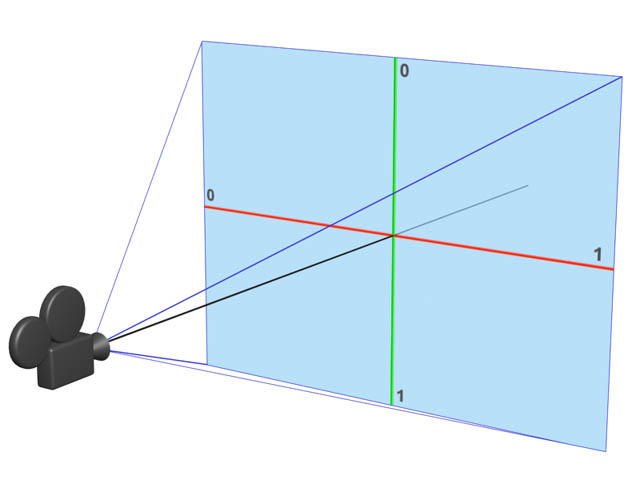
\includegraphics[width=9cm]{pics/camera01}
\end{center}
\end{methoddesc}

\begin{methoddesc}{getNearFar}{}
Return a 2-tuple (\var{near}, \var{far}) with the distances to the
near and far clipping planes. If automatic computation is disabled,
the method just returns the stored values, otherwise the values
are computed from the bounding box of the scene (which is converted
to a bounding sphere and the clipping planes are set as tangent planes
to the sphere).
\end{methoddesc}

% FreeCamera

\section{\class{FreeCamera} ---
         Free camera}

The \class{FreeCamera} class can be freely positioned and oriented in 
the scene.

\begin{classdesc}{FreeCamera}{name = "FreeCamera",\\ 
                       fov = 45.0,\\
                       target = None,\\
                       focallength = 0,\\
                       fstop = 0,\\
                       auto_nearfar = True,\\
                       nearplane = 0.1,\\
                       farplane = 1000.0,\\
                       }

\var{fov} is the field of view in degrees (in vertical direction), i.e.
the angle between the bottom and the top of the screen.

\var{target} is the point that the camera will initially look at. If no
target is specified the camera remains in its default orientation. Note
that the target is only used to compute an initial orientation. The
orientation will not be updated if the camera moves (use a 
\class{TargetCamera} if you want that behavior).

\var{focallength} is the focal length of the camera and \var{fstop} the
aperture number that determines the lens diameter. These values are used
to turn on depth of field. Depth of field is activated if both attributes
are set to a value different from 0 (note however, that not every renderer
supports depth of field). The focal distance is set so that the target 
point will always be in focus.

\var{auto_nearfar} specifies whether the near and far plane
distances are automatically determined or if fixed values are used.
If set to \code{False}, the \var{nearplane} and \var{farplane} arguments
are used, otherwise the values are computed from the objects in the scene.
In the latter case, the \var{nearplane} value still serves as minimum
value for the near plane distance which is used when the camera is located
within the scene bounds.
\end{classdesc}

The \class{FreeCamera} class has the following slots (in addition to
the slots of the \class{WorldObject} base class):

\begin{tableiv}{l|l|c|l}{code}{Slot}{Type}{Access}{Description}
\lineiv{fov_slot}{float}{rw}{Field of view in degrees}
\lineiv{focallength_slot}{float}{rw}{Focal length of the camera}
\lineiv{fstop_slot}{float}{rw}{Aperture number}
\lineiv{autonearfar_slot}{bool}{rw}{Automatically compute near/far values?}
\lineiv{nearplane_slot}{float}{rw}{(Minimal) near plane distance}
\lineiv{farplane_slot}{float}{rw}{Far plane distance}
\end{tableiv}

\begin{methoddesc}{projection}{width, height, near, far}
Returns the projection matrix for a viewport with the given width and
height (actually only the ratio width/height is relevant). The near
and far clipping planes are set to \var{near} and \var{far}.
\end{methoddesc}

\begin{methoddesc}{viewTransformation}{}
Returns the view transformation for this camera.
\end{methoddesc}

\begin{methoddesc}{eyeRay}{x0, y0, width, height}
Return a ray whose origin is at the eye position and that goes through
a given point on the image plane. The point on the plane is given by
(\var{x0}, \var{y0}) which each ranges from 0 to 1. (0,0) is at the
upper left and (1,1) at the lower right corner. The arguments \var{width} and
\var{height} determine the ratio of the image plane (the absolute
values of \var{width} and
\var{height} are irrelevant). The return value is a 2-tuple (\var{p}, \var{u})
where \var{p} is the ray origin and \var{u} the normalized
direction. Both vectors are given in world space.

\begin{center}
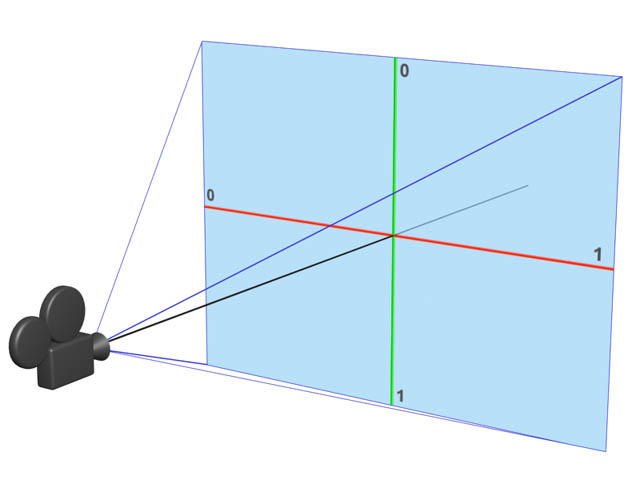
\includegraphics[width=9cm]{pics/camera01}
\end{center}
\end{methoddesc}

\begin{methoddesc}{getNearFar}{}
Return a 2-tuple (\var{near}, \var{far}) with the distances to the
near and far clipping planes. If automatic computation is disabled,
the method just returns the stored values, otherwise the values
are computed from the bounding box of the scene (which is converted
to a bounding sphere and the clipping planes are set as tangent planes
to the sphere).
\end{methoddesc}

% GLPointLight

\section{\class{GLPointLight} ---
         OpenGL point light}

\begin{classdesc}{GLPointLight}{name = ''GLPointLight'',\\ 
                       intensity = 1.0,\\
                       ambient = None,\\
                       diffuse = None,\\
                       specular = None,\\
                       constant_attenuation = 1.0,\\
                       linear_attenuation = 0.0,\\
                       quadratic_attenuation = 0.0,\\
                       enabled = True,\\
                       cast_shadow = False,\\
                       transform = None,\\
                       pos = None,\\
                       rot = None,\\
                       scale = None,\\
                       pivot = None,\\
                       offsetTransform = None,\\
                       auto_insert = True}

\end{classdesc}



% GLTargetSpotLight

\section{\class{GLTargetSpotLight} ---
         OpenGL target spot light}

\begin{classdesc}{GLTargetSpotLight}{name = ''GLTargetSpotLight'',\\ 
                       intensity = 1.0,\\
                       ambient = None,\\
                       diffuse = None,\\
                       specular = None,\\
                       constant_attenuation = 1.0,\\
                       linear_attenuation = 0.0,\\
                       quadratic_attenuation = 0.0,\\
                       exponent = 0.0,\\
                       cutoff = 45.0,\\
                       target = (0,0,0),\\
                       enabled = True,\\
                       cast_shadow = False,\\
                       transform = None,\\
                       pos = None,\\
                       rot = None,\\
                       scale = None,\\
                       pivot = None,\\
                       offsetTransform = None,\\
                       auto_insert = True}

\end{classdesc}



% GLFreeSpotLight

\section{\class{GLFreeSpotLight} ---
         OpenGL spot light}

\begin{classdesc}{GLFreeSpotLight}{name = ''GLFreeSpotLight'',\\ 
                       intensity = 1.0,\\
                       ambient = None,\\
                       diffuse = None,\\
                       specular = None,\\
                       constant_attenuation = 1.0,\\
                       linear_attenuation = 0.0,\\
                       quadratic_attenuation = 0.0,\\
                       exponent = 0.0,\\
                       cutoff = 45.0,\\
                       enabled = True,\\
                       cast_shadow = False,\\
                       transform = None,\\
                       pos = None,\\
                       rot = None,\\
                       scale = None,\\
                       pivot = None,\\
                       offsetTransform = None,\\
                       auto_insert = True}

\end{classdesc}



% GLTargetDistantLight

\section{\class{GLTargetDistantLight} ---
         OpenGL target distant light}

\begin{classdesc}{GLTargetDistantLight}{name = ''GLTargetDistantLight'',\\ 
                       intensity = 1.0,\\
                       ambient = None,\\
                       diffuse = None,\\
                       specular = None,\\
                       target = (0,0,0),\\
                       enabled = True,\\
                       cast_shadow = False,\\
                       transform = None,\\
                       pos = None,\\
                       rot = None,\\
                       scale = None,\\
                       pivot = None,\\
                       offsetTransform = None,\\
                       auto_insert = True}

\end{classdesc}



% GLFreeDistantLight

\section{\class{GLFreeDistantLight} ---
         OpenGL distant light}

\begin{classdesc}{GLFreeDistantLight}{name = ''GLFreeDistantLight'',\\ 
                       intensity = 1.0,\\
                       ambient = None,\\
                       diffuse = None,\\
                       specular = None,\\
                       enabled = True,\\
                       cast_shadow = False,\\
                       transform = None,\\
                       pos = None,\\
                       rot = None,\\
                       scale = None,\\
                       pivot = None,\\
                       offsetTransform = None,\\
                       auto_insert = True}

\end{classdesc}



% SpotLight3DS

\section{\class{SpotLight3DS} ---
         3DS spot light}

The \class{SpotLight3DS} class stores all parameters of the spot lights
as they are stored in 3DS files. The main purpose of this class is to
ensure that data doesn't get lost during file conversions.

This light sources can also be used for RenderMan renderings. However,
not all of the parameters are currently taken into account in the
corresponding RenderMan shader (see below).

\begin{classdesc}{SpotLight3DS}{name = "SpotLight3DS",\\ 
                       enabled = True,\\
                       intensity = 1.0,\\
                       color = (1,1,1),\\
                       see_cone = False,\\
                       roll = 0.0,\\
                       outer_range = 0,\\
                       inner_range = 0,\\
                       attenuation = 0,\\
                       rectangular_spot = 0,\\
                       shadowed = False,\\
                       shadow_bias = 0,\\
                       shadow_filter = 4.0,\\
                       shadow_size = 256,\\
                       spot_aspect = 0,\\
                       use_projector = False,\\
                       projector = 0,\\
                       overshoot = False,\\
                       ray_shadows = False,\\
                       ray_bias = False,\\
                       hotspot = 43,\\
                       falloff = 45,\\
	               target = (0,0,0)
                  }

\var{enabled} is a boolean flag that can be used to turn the light source
on or off.

\var{intensity} is the overall intensity of the light source. The higher
the value, the brighter the light.

\var{color} defines the color of the light source. It must be a sequence
of 3 floats containing RGB values.

\var{see_cone} ...

\var{roll} ...

\var{inner_range} and \var{outer_range} specify an intensity range based
on distance. Any parts of the scene that are nearer to the light source
than \var{inner_range} are fully illuminated. Within the range between
\var{inner_range} and \var{outer_range} the brightness drops off to 0
and objects further than \var{outer_range} are not illuminated at all.
These range values are only taken into account when \var{attenuation}
is not 0.

\var{rectangular_spot} ...

If \var{shadowed} is set to \code{True} the light casts a shadow.

\var{shadow_bias} is a small value greater than 0 that is used to prevent
invalid self-shadowing (i.e. so that a surface element doesn't shadow itself).

\var{shadow_filter} specifies the size of the filter when doing shadow map
lookups. The higher the value the blurrier the shadow.

\var{shadow_size} defines the size of the shadow map. The shadow map will
always be square and have a width of \var{shadow_size} pixels.

\var{spot_aspect} ...

\var{use_projector} ...

\var{projector} ...

If \var{overshoot} is \code{True} the light virtually becomes a point light
source, i.e. it also illuminates the parts of the scene that lie outside
its cone but the shadow is still restricted to the cone.

\var{ray_shadows} ...

\var{ray_bias} ...

\var{hotspot} This is the angle (in degrees) of the "inner" cone which is fully illuminated.

\var{falloff} This is the angle (in degrees) of the "outer" cone. The light 
intensity between the inner and outer cone drops off to 0. The region outside
the outer cone is not illuminated (unless \var{overshoot} is activated).

\var{target} is the target point that the light source aims at.

\end{classdesc}

The following parameters are used in the corresponding RenderMan
shader, all other parameters are currently ignored:

\begin{itemize}
\item intensity
\item color
\item falloff
\item hotspot
\item attenuation
\item inner_range
\item outer_range
\item overshoot
\item shadow_bias
\item shadow_filter
\item shadow_size
\end{itemize}

% MayaSpotLight

\section{\class{MayaSpotLight} ---
         Maya spot light}

\begin{classdesc}{MayaSpotLight}{name = "MayaSpotLight",\\ 
                       enabled = True,\\
                       color = (1,1,1),\\
                       intensity = 1.0,\\
                       decayRate = 0,\\
                       coneAngle = 40,\\
                       penumbraAngle = 40,\\
                       dropoff = 0,\\
                       useDepthMapShadows = False,\\
                       dmapResolution = 512,\\
                       useMidDistDmap = True,\\
                       useDmapAutoFocus = True,\\
                       dmapFocus = 90.0,\\
                       dmapFilterSize = 1,\\
                       dmapBias = 0.001,\\
	               target = (0,0,0)
                  }

\var{enabled} is a boolean flag that can be used to turn the light source
on or off.

\var{intensity} is the overall intensity of the light source. The higher
the value, the brighter the light.

\var{color} defines the color of the light source. It must be a sequence
of 3 floats containing RGB values.

...

\var{target} is the target point that the light source aims at.

\end{classdesc}


% SpotLight3DS

\section{\class{RMLightSource} ---
         RenderMan light source}

\begin{classdesc}{RMLightSource}{name = "RMLightSource",\\ 
                       shader = None
                  }


\var{shader} specifies the light shader that should be used. It
can either be a string containing the shader name or a \class{RMShader}
instance representing the shader (see section \ref{rmshader}).

\end{classdesc}


The parameters of the shader is made available as attributes of the
light source object. The corresponding slots can be obtained by adding
the suffix \code{_slot} to the name.


% RIBArchive component

\section{\class{RIBArchive} ---
         Reference an external RIB archive}

The \class{RIBArchive} class represents geometry that is defined in
an external RIB file. When the scene is rendered using a RenderMan
renderer the RIB file will be included via a call to 
\cfunction{RiReadArchive()}. In an interactive viewer, a \class{RIBArchive}
object will be invisible.

\begin{classdesc}{RIBArchive}{name = "RIBArchive",\\ 
                              filename = None, \\
                              auto_insert = True}

\var{filename} is the name of the external RIB file.

\end{classdesc}



% ODE joints

\section{ODE joints ---
         Joint classes for the ODEDynamics component}

%----------------------------------------------------------------------
\subsection{\class{ODEBallJoint} --- Ball and socket joint}

\begin{classdesc}{ODEBallJoint}{name = "ODEBallJoint",\\ 
                             body1 = None, \\
                             body2 = None
                             }

\end{classdesc}

%----------------------------------------------------------------------
\subsection{\class{ODEHingeJoint} --- Hinge joint}

\begin{classdesc}{ODEHingeJoint}{name = "ODEHingeJoint",\\ 
                             body1 = None, \\
                             body2 = None
                             }

\end{classdesc}

%----------------------------------------------------------------------
\subsection{\class{ODESliderJoint} --- Slider joint}

\begin{classdesc}{ODESliderJoint}{name = "ODESliderJoint",\\ 
                             body1 = None, \\
                             body2 = None
                             }

\end{classdesc}

%----------------------------------------------------------------------
\subsection{\class{ODEHinge2Joint} --- Hinge-2 joint}

\begin{classdesc}{ODEHinge2Joint}{name = "ODEHinge2Joint",\\ 
                             body1 = None, \\
                             body2 = None
                             }

\end{classdesc}

%----------------------------------------------------------------------
\subsection{\class{ODEUniversalJoint} --- Universal joint}

\begin{classdesc}{ODEUniversalJoint}{name = "ODEUniversalJoint",\\ 
                             body1 = None, \\
                             body2 = None
                             }

\end{classdesc}




% BezierCurve

\section{\class{BezierCurve} ---
         Bezier curve}

\begin{classdesc}{BezierCurve}{name = "BezierCurve",\\ 
                               pnts = None,\\
                               closed = False,\\
                               epsilon = 0.01,\\
                               subdiv = 4,\\
                               show_tangents = False,\\
                               curvegeom = None\\
                              }

\var{pnts} is a list of \class{BezierPoint} objects (see section
\ref{beziercurvegeom}).

If \var{closed} is set to \code{True} the last point will be connected
to the first point.

\var{epsilon} is a threshold value that determines the accuracy of
length calculations of the curve.

\var{subdiv} is the number of subdivisions that are made to draw the
curve using OpenGL.

If \var{show_tangents} is set to \code{True} the OpenGL visualization
will also show the in and out tangents.

You can also pass a previously created \class{BezierCurveGeom} object
via the \var{curvegeom} argument. In this case, the arguments \var{pnts},
\var{closed}, \var{epsilon}, \var{subdiv} and \var{show_tangents} are 
ignored.
\end{classdesc}





%---
\chapter{GeomObjects \label{geomobjects}}

% GeomObject

\section{\class{GeomObject} ---
         Geometry base class}

The \class{GeomObject} class is the base class for all geometries.
Instances of this class are stored in the \member{geom} attribute
of the world objects and can be shared among them.

\begin{classdesc}{GeomObject}{}
...params?...
\end{classdesc}

% Methods
\begin{methoddesc}{boundingBox}{}
Return the local axis aligned bounding box. The bounding box is
given with respect to the local transformation L (which is not
what you get from the transform slot of the world object).
\end{methoddesc}

\begin{methoddesc}{drawGL}{}
Draw the geometry using OpenGL commands.
\end{methoddesc}

\begin{methoddesc}{uniformCount}{}
Return the multiplicity of \keyword{UNIFORM} variables.
\end{methoddesc}

\begin{methoddesc}{varyingCount}{}
Return the multiplicity of \keyword{VARYING} variables.
\end{methoddesc}

\begin{methoddesc}{vertexCount}{}
Return the multiplicity of \keyword{VERTEX} variables.
\end{methoddesc}

\begin{methoddesc}{faceVaryingCount}{}
Return the multiplicity of \keyword{FACEVARYING} variables.
\end{methoddesc}

\begin{methoddesc}{faceVertexCount}{}
Return the multiplicity of \keyword{FACEVERTEX} variables.
\end{methoddesc}

\begin{methoddesc}{slotSizeConstraint}{storage}
Return a constraint object for primitive variable slots or None if the size
of the slot should be unconstrained.
This method is called when a new primitive variable is created. The
returned constraint object is used for the array slot that holds the
values of the variable. \var{storage} is the storage class of the new
variable which will be one of \code{UNIFORM}, \code{VARYING}, \code{VERTEX},
\code{FACEVARYING} or \code{FACEVERTEX}. The method will never be called
when \code{CONSTANT} or \code{USER} variables are created.
\end{methoddesc}

\begin{methoddesc}{newVariable}{name, storage, type, multiplicity=1, user_n=0}
Attaches a new primitive variable to the geometry.

\var{storage} specifies the storage
class, i.e. how many values are actually stored. It must be one of
\code{CONSTANT}, \code{UNIFORM}, \code{VARYING}, \code{VERTEX}, 
\code{FACEVARYING}, \code{FACEVERTEX} or
\code{USER}. The exact number of values depends on the actual geometry.
However, \code{CONSTANT} is always exactly one value for the entire
geometry and \code{USER} is a user defined number specified in \var{user_n}.

\var{type} is the type of the variable and must be one of 
\code{INT}, \code{FLOAT}, \code{STRING}, \code{COLOR}, \code{POINT}, 
\code{VECTOR}, \code{NORMAL}, \code{MATRIX} and \code{HPOINT}. 
If \var{multiplicity} is greater than 1, then an array with that size is
created. 

Creating a new variable will always create a new slot of that name as well.
The slot is always an \class{ArraySlot} (even for \code{CONSTANT} variables).
After you have created a variable you can use the corresponding slot to
manipulate the values of the variable.

Here is an example of a "varying int [3]" variable that's created on a sphere 
geometry. This means, the variable will consist of four 3-tuples of integers
(one for each parametric corner).

\begin{verbatim}
>>> from cgkit.all import *
>>> sg=SphereGeom()
>>> sg.newVariable("foo", VARYING, INT, multiplicity=3)
>>> for v in sg.iterVariables(): print v
...
('foo', cgkit._core.VarStorage.VARYING, cgkit._core.VarType.INT, 3)
>>> s=sg.slot("foo")
>>> s[1]=(1,2,3)
>>> for f in s: print f
...
(0, 0, 0)
(1, 2, 3)
(0, 0, 0)
(0, 0, 0)
\end{verbatim}
\end{methoddesc}

\begin{methoddesc}{deleteVariable}{name}
Delete the primitive variable with the specified name.
\end{methoddesc}

\begin{methoddesc}{deleteAllVariables}{}
Delete all primitive variables.
\end{methoddesc}

\begin{methoddesc}{findVariable}{name}
Search for a particular primitive variable and return its descriptor.
\code{None} is returned if a variable called \var{name} cannot be found.
The return value is a 4-tuple (name, storage class, type, multiplicity)
describing the variable. See the \method{newVariable()} method for a
description of the individual elements.
\end{methoddesc}

\begin{methoddesc}{iterVariables}{}
Return an iterator that iterates over all existing primitive variables.
The iterator will return the same 4-tuple as returned by 
\method{findVariable()}.
\end{methoddesc}

\begin{methoddesc}{convert}{targetgeom}
Convert the geometry into another type of geometry. \var{targetgeom}
is another \class{GeomObject} that will receive the result of the
conversion.  If the conversion is not possible, a
\exception{NotImplementedError} exception is thrown.

In the following example, a box geometry is converted into a triangle
mesh:

\begin{verbatim}
>>> bg=BoxGeom(segmentsx=3, segmentsy=3, segmentsz=3)
>>> tm=TriMeshGeom()
>>> bg.convert(tm)
>>> print len(tm.verts)
56
>>> print len(tm.faces)
108
\end{verbatim}
\end{methoddesc}




% BoxGeom

\section{\class{BoxGeom} ---
         Box geometry}

\begin{classdesc}{BoxGeom}{lx=1.0, ly=1.0, lz=1.0, segmentsx=1, segmentsy=1, segmentsz=1}

\var{lx}, \var{ly} and \var{lz} specify the dimensions of the box in
the respective direction.

\var{segmentsx}, \var{segmentsy} and \var{segmentsz} are the number of
segments in each direction.
\end{classdesc}

A \class{BoxGeom} has the following slots:

\begin{tableiv}{l|l|c|l}{code}{Slot}{Type}{Access}{Description}
\lineiv{cog_slot}{vec3}{r}{The local center of gravity}
\lineiv{inertiatensor_slot}{mat3}{r}{The local inertia tensor}
\lineiv{lx_slot}{float}{rw}{The length in x direction}
\lineiv{ly_slot}{float}{rw}{The length in y direction}
\lineiv{lz_slot}{float}{rw}{The length in z direction}
\lineiv{segmentsx_slot}{int}{rw}{The number of segments in x direction}
\lineiv{segmentsy_slot}{int}{rw}{The number of segments in y direction}
\lineiv{segmentsz_slot}{int}{rw}{The number of segments in z direction}
\end{tableiv}

% Attributes
\begin{memberdesc}{cog}
Center of gravity with respect to the local coordinate system.
\end{memberdesc}

\begin{memberdesc}{inertiatensor}
Inertia tensor with respect to the local coordinate system.
\end{memberdesc}

\begin{memberdesc}{lx}
The length in x direction.
\end{memberdesc}

\begin{memberdesc}{ly}
The length in y direction.
\end{memberdesc}

\begin{memberdesc}{lz}
The length in z direction.
\end{memberdesc}

\begin{memberdesc}{segmentsx}
The number of segments in x direction.
\end{memberdesc}

\begin{memberdesc}{segmentsy}
The number of segments in y direction.
\end{memberdesc}

\begin{memberdesc}{segmentsz}
The number of segments in z direction.
\end{memberdesc}








% SphereGeom

\section{\class{SphereGeom} ---
         Sphere geometry}

\begin{classdesc}{SphereGeom}{radius=1.0, segmentsu=16, segmentsv=8}
\var{radius} is the radius in the local coordinate system.

\var{segmentsu} and \var{segmentsv} are used when the sphere has to
be tesselated (either for interactive display or when converted to
a triangle mesh).
\end{classdesc}

A \class{SphereGeom} has the following slots:

\begin{tableiv}{l|l|c|l}{code}{Slot}{Type}{Access}{Description}
\lineiv{cog_slot}{vec3}{r}{The local center of gravity}
\lineiv{inertiatensor_slot}{mat3}{r}{The local inertia tensor}
\lineiv{radius_slot}{float}{rw}{The radius}
\lineiv{segmentsu_slot}{int}{rw}{The number of segments in u direction}
\lineiv{segmentsv_slot}{int}{rw}{The number of segments in v direction}
\end{tableiv}

% Attributes
\begin{memberdesc}{cog}
Center of gravity with respect to the local coordinate system.
\end{memberdesc}

\begin{memberdesc}{inertiatensor}
Inertia tensor with respect to the local coordinate system.
\end{memberdesc}

\begin{memberdesc}{radius}
The radius of the sphere.
\end{memberdesc}

\begin{memberdesc}{segmentsu}
The number of segments in u direction.
\end{memberdesc}

\begin{memberdesc}{segmentsv}
The number of segments in v direction.
\end{memberdesc}







% CCylinderGeom

\section{\class{CCylinderGeom} ---
         Capped cylinder geometry}

\begin{classdesc}{CCylinderGeom}{radius=1.0, length=1.0, segmentsu=16, segmentsvl=1, segmentsvr=4}

\var{radius} is the radius of the cylinder and caps in the local coordinate 
system.

\var{length} is the length of the cylinder (not counting the caps).

\var{segmentsu} is the number of segments in u direction, \var{segmentsvl}
the number of segments of the cylinder part and \var{segmentsvr} the
number of segments for each cap.
\end{classdesc}

A \class{CCylinderGeom} has the following slots:

\begin{tableiv}{l|l|c|l}{code}{Slot}{Type}{Access}{Description}
\lineiv{cog_slot}{vec3}{r}{The local center of gravity}
\lineiv{inertiatensor_slot}{mat3}{r}{The local inertia tensor}
\lineiv{radius_slot}{float}{rw}{The radius of the cylinder}
\lineiv{length_slot}{float}{rw}{The lenght of the cylinder}
\lineiv{segmentsu_slot}{int}{rw}{The number of segments in u direction}
\lineiv{segmentsvl_slot}{int}{rw}{The number of cylinder segments in v direction}
\lineiv{segmentsvr_slot}{int}{rw}{The number of cap segments in v direction}
\end{tableiv}

% Attributes
\begin{memberdesc}{cog}
Center of gravity with respect to the local coordinate system.
\end{memberdesc}

\begin{memberdesc}{inertiatensor}
Inertia tensor with respect to the local coordinate system.
\end{memberdesc}

\begin{memberdesc}{radius}
The radius of the cylinder and caps.
\end{memberdesc}

\begin{memberdesc}{length}
The length of the cylinder (not counting the caps).
\end{memberdesc}

\begin{memberdesc}{segmentsu}
The number of segments in u direction.
\end{memberdesc}

\begin{memberdesc}{segmentsvl}
The number of cylinder segments in v direction.
\end{memberdesc}

\begin{memberdesc}{segmentsvr}
The number of cap segments in v direction.
\end{memberdesc}

% PlaneGeom

\section{\class{PlaneGeom} ---
         Plane geometry}

\begin{classdesc}{PlaneGeom}{lx=1.0, ly=1.0, segmentsx=1, segmentsy=1}

\var{lx} and \var{ly} specify the dimensions of the plane in
the respective direction.

\var{segmentsx} and \var{segmentsy} are the number of
segments in each direction.
\end{classdesc}

A \class{PlaneGeom} has the following slots:

\begin{tableiv}{l|l|c|l}{code}{Slot}{Type}{Access}{Description}
\lineiv{lx_slot}{float}{rw}{The length in x direction}
\lineiv{ly_slot}{float}{rw}{The length in y direction}
\lineiv{segmentsx_slot}{int}{rw}{The number of segments in x direction}
\lineiv{segmentsy_slot}{int}{rw}{The number of segments in y direction}
\end{tableiv}

% Attributes
\begin{memberdesc}{lx}
The length in x direction.
\end{memberdesc}

\begin{memberdesc}{ly}
The length in y direction.
\end{memberdesc}

\begin{memberdesc}{segmentsx}
The number of segments in x direction.
\end{memberdesc}

\begin{memberdesc}{segmentsy}
The number of segments in y direction.
\end{memberdesc}







% TorusGeom

\section{\class{TorusGeom} ---
         Torus geometry}

\begin{classdesc}{TorusGeom}{major=1.0, minor=0.1, segmentsu=16, segmentsv=8}
\end{classdesc}








% TriMeshGeom

\section{\class{TriMeshGeom} ---
         Triangle mesh geometry}

\begin{classdesc}{TriMeshGeom}{}
Creates an empty triangle mesh.
\end{classdesc}

A \class{TriMeshGeom} has the following slots:

\begin{tableiv}{l|l|c|l}{code}{Slot}{Type}{Access}{Description}
\lineiv{cog_slot}{vec3}{r}{The local center of gravity}
\lineiv{inertiatensor_slot}{mat3}{r}{The local inertia tensor}
\lineiv{verts_slot}{vec3 array}{rw}{The mesh vertices}
\lineiv{faces_slot}{int[3] array}{rw}{The mesh faces}
\end{tableiv}

% Attributes
\begin{memberdesc}{cog}
Center of gravity with respect to the local coordinate system of the 
triangle mesh.
\end{memberdesc}

\begin{memberdesc}{inertiatensor}
Inertia tensor with respect to the local coordinate system of the 
triangle mesh.
\end{memberdesc}

\begin{memberdesc}{verts}
This attribute contains the sequence of mesh vertices.
\end{memberdesc}

\begin{memberdesc}{faces}
This attribute contains the sequence of mesh faces. Each face contains
three vertex indices.
\end{memberdesc}

% Methods
\begin{methoddesc}{intersectRay}{origin, direction, earlyexit=False}
Intersect a ray with the mesh. The ray starts at \var{origin} and
travels along \var{direction} which must both be of type \class{vec3}.
\var{origin} and \var{direction} must be given with respect to the
local coordinate system L of the geometry. If \var{earlyexit} is
\code{True} the method returns after the first hit, otherwise all
triangles are tested and the result contains the nearest hit.
The return value is a tuple (\var{hit}, \var{t}, \var{faceindex}, 
\var{u}, \var{v}) where \var{hit} is a boolean that indicates if
the mesh was hit or not. \var{t} is the ray parameter, i.e. the
point of intersection is at \var{origin} + t*\var{direction}.
\var{faceindex} is the index of the face that was hit and \var{u}
\var{v} are the parameter coordinates of the intersection point.

This method tests the ray with all triangles, so it is not efficient if
you have a lot of rays to test. It is meant for only a few rays where
the preprocessing cost wouldn't be amortized.
 
The ray-triangle intersection code (non-culling case) is based on:
 
Tomas M�ller and Ben Trumbore\\
{\em Fast, minimum storage ray-triangle intersection}\\
Journal of graphics tools, 2(1):21-28, 1997\\
\url{http://www.acm.org/jgt/papers/MollerTrumbore97/}
\end{methoddesc}






% PolyhedronGeom

\section{\class{PolyhedronGeom} ---
         Polyhedron geometry}

The \class{PolyhedronGeom} class stores a collection of general planar
concave polygons that may also contain holes. Each polygon is described
by a sequence of vertex loops. The first loop defines the polygon boundary
and each subsequent loop describes a hole. Each loop is a sequence of
vertex indices.

\begin{classdesc}{PolyhedronGeom}{}
Creates an empty polyhedron.
\end{classdesc}

A \class{PolyhedronGeom} has the following slots:

\begin{tableiv}{l|l|c|l}{code}{Slot}{Type}{Access}{Description}
\lineiv{verts_slot}{vec3 array}{rw}{The polygon vertices}
\end{tableiv}

% Attributes
\begin{memberdesc}{verts}
This attribute contains the sequence of polygon vertices.
\end{memberdesc}

% Methods
\begin{methoddesc}{hasPolysWithHoles}{}
Return \code{True} if there is at least one polygon with a hole.
\end{methoddesc}

\begin{methoddesc}{getNumPolys}{}
Return the number of polygons.
\end{methoddesc}

\begin{methoddesc}{getNumLoops}{poly}
Return the number of vertex loops in the polygon with index \var{poly}.
\end{methoddesc}

\begin{methoddesc}{getNumVerts}{poly, loop}
Return the number of vertex indices in one particular loop. \var{poly}
is the polygon index and \var{loop} the loop index.
\end{methoddesc}

\begin{methoddesc}{setNumPolys}{num}
Allocate space for \var{num} polygons.
\end{methoddesc}

\begin{methoddesc}{setNumLoops}{poly, num}
Allocate space for \var{num} loops in the polygon with index \var{poly}.
\end{methoddesc}

\begin{methoddesc}{getLoop}{poly, loop}
Return a loop from a polygon. \var{poly} is the polygon index and \var{loop}
the loop index. The return value is a sequence of vertex indices.
\end{methoddesc}

\begin{methoddesc}{setLoop}{poly, loop, vloop}
Set a new polygon loop. \var{poly} is the polygon index, \var{loop}
the loop index and \var{vloop} a sequence of vertex indices.
\end{methoddesc}

\begin{methoddesc}{getPoly}{poly}
Return a polygon. \var{poly} is the polygon index. The return value
is a sequence of vertex loops.
\end{methoddesc}

\begin{methoddesc}{setPoly}{poly, polydef}
Set a polygon. \var{poly} is the polygon index and \var{polydef} a sequence
of vertex loops.
\end{methoddesc}





% BezierCurveGeom

\section{\class{BezierCurveGeom} ---
         Piecewise cubic Bezier curve}
\label{beziercurvegeom}

The \class{BezierCurveGeom} class represents a piecewise cubic curve
in 3D space that is composed of an arbitrary number of cubic Bezier
segments. The class stores a number of 3D points that are interpolated
by the curve. Each point has an in tangent and an out tangent associated
with it that define how the curve enters and leaves the point.

\begin{classdesc}{BezierPoint}{pos, intangent=vec3(0), outtangent=vec3(0)}

This class just stores a position and the in and out tangents and
is used to pass these parameters to the constructor of a 
\class{BezierCurveGeom}.

\var{pos} is a point position that the curve will interpolate.

\var{intangent} and \var{outtangent} define where the curve enters
and leaves the point.
\end{classdesc}


\begin{classdesc}{BezierCurveGeom}{pnts = None,\\
                                   closed = False,\\
                                   epsilon = 0.01,\\
                                   subdiv = 4,\\
                                   show_tangents = False}

\var{pnts} is a list of \class{BezierPoint} objects describing the
points to interpolate and the in and out tangents.

If \var{closed} is set to \code{True} the last point will be connected
to the first point.

\var{epsilon} is a threshold value that determines the accuracy of
length calculations of the curve.

\var{subdiv} is the number of subdivisions that are made to draw the
curve using OpenGL.

If \var{show_tangents} is set to \code{True} the OpenGL visualization
will also show the in and out tangents.
\end{classdesc}

A \class{BezierCurveGeom} has the following slots:

\begin{tableiv}{l|l|c|l}{code}{Slot}{Type}{Access}{Description}
\lineiv{pnts_slot}{[vec3]}{rw}{The curve points}
\lineiv{intangents_slot}{[vec3]}{rw}{The in tangents}
\lineiv{outtangents_slot}{[vec3]}{rw}{The out tangents}
\end{tableiv}

\begin{memberdesc}{closed}
This is a boolean indicating wheter the curve is closed or not. You
can read and write this attribute.
\end{memberdesc}

\begin{memberdesc}{numsegs}
The number of Bezier segments in the curve. You can only read this
attribute.
\end{memberdesc}

\begin{memberdesc}{paraminterval}
This is a tuple (\var{t_min}, \var{t_max}) containing the valid parameter
interval of the curve. You can only read this attribute.
\end{memberdesc}

% eval
\begin{methoddesc}{eval}{t}
Evaluate the curve at parameter \var{t} and return the curve point.
\end{methoddesc}

% evalFrame
\begin{methoddesc}{evalFrame}{t}
Evaluate the curve at parameter \var{t} and return the curve point,
the tangent and the second derivative.
\end{methoddesc}

% deriv
\begin{methoddesc}{deriv}{t}
Return the first derivative (the tangent) at parameter \var{t}.
\end{methoddesc}

% arcLen
\begin{methoddesc}{arcLen}{t}
Return the arc length of the curve up to the point specified by the parameter
\var{t}.
\end{methoddesc}

% length
\begin{methoddesc}{length}{}
Return the entire length of the curve. This is equivalent to 
\code{arcLen(t_max)}.
\end{methoddesc}








%---
\chapter{Materials \label{materials}}

% GLMaterial

\section{\class{GLMaterial} ---
         OpenGL material}

The \class{GLMaterial} class represents the material model of the standard
OpenGL API. All colors are represented as (r,g,b,a). If you don't use
blending you can leave out the alpha value in the constructor.

\begin{classdesc}{GLMaterial}{name = "GLMaterial",\\ 
                              ambient = (0.2, 0.2, 0.2, 1.0),\\
                              diffuse = (0.7, 0.7, 0.7, 1.0),\\
                              specular = (0, 0, 0, 1),\\
                              shininess = 0.0,\\
                              emission = (0, 0, 0, 1),\\
                              blend_factors = None,\\
                              texture = None,\\
                              vertex_shader = None,\\
                              fragment_shader = None,\\
                              density = 1.0}

\var{ambient} is the ambient color of the material.

\var{diffuse} is the diffuse color of the material.

\var{specular} is the color of the specular highlight.

\var{shininess} determines the size of the highlight and lies 
between 0.0 and 128.0. The higher the value, the smaller and brighter
the highlight.

The \var{emission} color can be used to simulate objects that emit light.

\var{blend_factors} is a 2-tuple with the parameters for the 
\cfunction{glBlendFunc()} call which indicate how to compute the
source and destination blend factors 
(see \ulink{\cfunction{glBlendFunc()}}{http://pyopengl.sourceforge.net/documentation/manual/glBlendFunc.3G.html}).
Blending is disabled if \var{blend_factors} is \code{None}.

\var{texture} is either \code{None}, a single \class{GLTexture} object or
a list of \class{GLTexture} objects specifying the texture image(s) to use.

\var{vertex_shader} is either \code{None}, a single \class{GLShader} object
or a list of \class{GLShader} objects specifying the vertex shaders to use.

\var{fragment_shader} is either \code{None}, a single \class{GLShader} object
or a list of \class{GLShader} objects specifying the fragment shaders to use.

\var{density} is the density value used for physical simulations.
\end{classdesc}

% Methods
\begin{methoddesc}{getNumTextures}{}
Return the current size of the texture array.
\end{methoddesc}

\begin{methoddesc}{setNumTextures}{num}
Set a new size for the texture array.
\end{methoddesc}

\begin{methoddesc}{getTexture}{idx=0}
Get a stored texture. The method returns \code{None} if the given index
is out of range or if there is no texture stored at that position.
\end{methoddesc}

\begin{methoddesc}{setTexture}{tex, idx=0}
Set a new texture. An \exception{IndexError} exception is thrown if the 
index is out of range.
\end{methoddesc}

\begin{methoddesc}{getNumVertexShaders}{}
Return the current size of the vertex shader array.
\end{methoddesc}

\begin{methoddesc}{setNumVertexShaders}{num}
Set a new size for the vertex shader array.
\end{methoddesc}

\begin{methoddesc}{getVertexShader}{idx=0}
Get a vertex shader object. The method returns \code{None} if the given index
is out of range or if there is no shader object stored at that position.
\end{methoddesc}

\begin{methoddesc}{setVertexShader}{shader, idx=0}
Set a new vertex shader object. An \exception{IndexError} exception is 
thrown if the index is out of range. A ValueError exception is thrown if the 
shader is not of type \code{VERTEX}.
\end{methoddesc}

\begin{methoddesc}{getNumFragmentShaders}{}
Return the current size of the fragment shader array.
\end{methoddesc}

\begin{methoddesc}{setNumFragmentShaders}{num}
Set a new size for the fragment shader array.
\end{methoddesc}

\begin{methoddesc}{getFragmentShader}{idx=0}
Get a fragment shader object. The method returns \code{None} if the given index
is out of range or if there is no shader object stored at that position.
\end{methoddesc}

\begin{methoddesc}{setFragmentShader}{shader, idx=0}
Set a new fragment shader object. An \exception{IndexError} exception is 
thrown if the index is out of range. A ValueError exception is thrown if the 
shader is not of type \code{FRAGMENT}.
\end{methoddesc}

%-----------------------
\subsection{\class{GLTexture} --- Specifying a texture map}

The \class{GLTexture} class is used to describe the parameters of an
OpenGL texture map for use with the \class{GLMaterial} class.

\begin{classdesc}{GLTexture}{imagename = "",\\
                             image = None,\\ 
                             mode = GL_DECAL,\\
                             mipmap = True,\\
                             mag_filter = GL_LINEAR,\\
                             min_filter = GL_LINEAR,\\
                             wrap_s = GL_REPEAT,\\
                             wrap_t = GL_REPEAT,\\
                             internalformat = GL_RGB,\\
                             texenvcolor = vec4(1),\\
                             transform = mat4(1),\\
                             size = None, \\
                             environment_map = False\\
                            }

\var{imagename} is the name of the image file that should be used as a
texture map. If the image resolution is not a power of 2, the image
is scaled up to the next higher power of 2 resolution.

It is also possible to pass the actual image data in the \var{image}
parameter.  The image can either be a PIL image or the raw RGB
data. In the latter case, you must explicitly specify the image
resolution (which must then be a power of 2 resolution) in the \var{size}
argument. The \var{imagename} argument is ignored if the data is passed
via the \var{image} argument.

\var{mode} specifies how the image is applied to the object. It can be
one of \code{GL_REPLACE}, \code{GL_MODULATE}, \code{GL_DECAL} and 
\code{GL_BLEND}. In the latter
case, the blend color is given by \var{texenvcolor} 
(see \ulink{\cfunction{glTexEnv()}}{http://pyopengl.sourceforge.net/documentation/manual/glTexEnv.3G.html}).

\var{mipmap} determines whether mip mapping should be used or not.

\var{mag_filter} is the filter to use when magnification occurs (i.e. when
the texture appears larger on screen that it actually is). It can be
either \code{GL_NEAREST} or \code{GL_LINEAR}.

\var{min_filter} is the filter to use when minification occurs (i.e. when
the texture appears smaller on screen that it actually is). It can be one
of following values
(see \ulink{\cfunction{glTexParameter()}}{http://pyopengl.sourceforge.net/documentation/manual/glTexParameter.3G.html}):
%\code{GL_NEAREST}, \code{GL_LINEAR}, \code{GL_NEAREST_MIPMAP_NEAREST},
%\code{GL_NEAREST_MIPMAP_LINEAR}, \code{GL_LINEAR_MIPMAP_NEAREST} or
%\code{GL_LINEAR_MIPMAP_LINEAR}

\begin{itemize}
\item \code{GL_NEAREST}
\item \code{GL_LINEAR}
\item \code{GL_NEAREST_MIPMAP_NEAREST}
\item \code{GL_NEAREST_MIPMAP_LINEAR}
\item \code{GL_LINEAR_MIPMAP_NEAREST}
\item \code{GL_LINEAR_MIPMAP_LINEAR}
\end{itemize}

If \code{GL_LINEAR} is specified and mip mapping
is used then the filter is automatically set to \code{GL_LINEAR_MIPMAP_LINEAR}

\var{wrap_s} and \var{wrap_t} specify what happens if the texture coordinate
leave the range 0-1. They can be one of \code{GL_REPEAT}, \code{GL_CLAMP}
and \code{GL_CLAMP_TO_EDGE}
(see \ulink{\cfunction{glTexParameter()}}{http://pyopengl.sourceforge.net/documentation/manual/glTexParameter.3G.html}).

\var{internalformat} specifies how the image data will be stored in memory.
Usually, you'll either specify \code{GL_RGB} or \code{GL_RGBA} if you have
alpha values in your image and you want to use them
(see \ulink{\cfunction{glTexImage2D()}}{http://pyopengl.sourceforge.net/documentation/manual/glTexImage2D.3G.html}).

\var{transform} is a transformation that is applied to the texture coordinates.

\var{size} is a 2-tuple containing the desired texture map resolution which
must be a power of 2. The image is resized to the specified resolution.
If \var{size} is \code{None} then the next higher power of 2 value is used.

If \var{environment_map} is \code{True} the image is used as a 
latitude/longitude environment map.

\end{classdesc}

%-----------------------
\subsection{\class{GLShader} --- Specifying a shader}

The \class{GLShader} class is used to add a OpenGL 2 shader source file
to a \class{GLMaterial} class.

\begin{classdesc}{GLShader}{shadertype,\\
                            filename,\\ 
                            cpp = None,\\
                            cpperrstream = sys.stderr,\\
                            **shaderparams
                            }

\var{shadertype} specifies whether this shader is vertex shader or a
fragment shader. The value can either be \code{GLShader.ShaderType.VERTEX}
(or \code{GLSLANG_VERTEX}) or \code{GLShader.ShaderType.FRAGMENT}
(or \code{GLSLANG_FRAGMENT}).

\var{filename} is the shader source file name.

\var{cpp} determines the preprocessor that should be used when extracting
shader parameters. \var{cpperrstream} is used to output errors from the
preprocessor (see the function \function{glslangparams.glslangparams()} 
(section \ref{glslangparams}) for details).

Any additional keyword argument is assumed to be a shader parameter.
\end{classdesc}


% RMMaterial

\section{\class{RMMaterial} ---
         RenderMan material}

The \class{RMMaterial} class is a special material that is only of
use if you are creating images via a RenderMan renderer and you want
to write your shaders in external shader files or use shaders that
are already compiled.

The material may consist of a surface shader, a displacement shader
and an interior shader. The shader source files (or only the shader
names) are passed via \class{RMShader} instances as arguments to the
constructor. If the \class{RMShader} instance points to a file, the
material object will take care of the compilation of the
file. Otherwise, it is up to you to compile the shader and make sure
that the renderer can find it.

\begin{classdesc}{RMMaterial}{name = "RMMaterial", \\
                              surface = None,\\
                              displacement = None,\\
                              displacementbound = ("current", 0.0),\\
                              interior = None,\\
                              color = None,\\
                              opacity = None
                             }


\var{surface} specifies the surface shader to use. It can either be
a string containing the shader name or a \class{RMShader} instance
representing the shader. You can also pass \code{None} if no surface
shader should be instantiated.

\var{displacment} specifies the displacment shader to use. It can either be
a string containing the shader name or a \class{RMShader} instance
representing the shader. You can also pass \code{None} if no displacment
shader should be instantiated.

\var{displacementbound} is a tuple (coordinate system, distance) that
specifies the maximum displacement. The distance is the maximum amount that
a surface point is displaced and  is given in the specified coordinate 
system.

\var{interior} specifies the interior shader to use. It can either be
a string containing the shader name or a \class{RMShader} instance
representing the shader. You can also pass \code{None} if no interior
shader should be instantiated.

\var{color} is the color that should be set via \cfunction{RiColor()}.

\var{opacity} is the opacity that should be set via \cfunction{RiOpacity()}.
\end{classdesc}

The parameters of the shaders are made available as attributes of the
material objects. The corresponding slots can be obtained by adding
the suffix \code{_slot} to the name. Attribute names in the surface shader
have priority over the attributes in the displacement shader which in
turn has priority over the interior shader. This means, if there are
identical parameter names in all shaders you will access the parameter
of the surface shader. You can also access the attributes of each
shader via the \var{surface}, \var{displacement} and \var{interior}
attributes which contain the corresponding \class{RMShader} instances.

Example:
   
\begin{verbatim}
mat = RMMaterial(surface = RMShader("mysurface.sl"),
                 displacement = RMShader("c:\\shaders\\dented.sl"),
                 color = (1,0.5,0.8)
                 )
...
Sphere(pos=(1,2,3), radius=0.5, material=mat)
\end{verbatim}

In this example, the material uses the surface shader \file{mysurface.sl}
and the displacement shader \file{c:\textbackslash shaders\textbackslash dented.sl}. The shaders will
be compiled automatically because the shader source files are given
(instead of just the shader names).

%------------------------------------------------------------
\subsection{\class{RMShader} ---  RenderMan shader}
\label{rmshader}

The \class{RMShader} class encapsulates a single RenderMan shader.

\begin{classdesc}{RMShader}{shader = None, \\
                            transform = mat4(1), \\
                            cpp = None, \\
                            cpperrstream = sys.stderr, \\
                            params = None, \\
                            paramlist}
	
\var{shader} is either the name of a shader or the shader source file.
If a shader file is given then the shader is read to extract the parameters.
Each parameter will be made available as slot.

\var{transform} is a \class{mat4} containing a transformation that should
be applied to the shader. This means you can transform the shader relative
to the object it is applied to.

\var{cpp} determines the preprocessor that should be used when extracting
parameters. \var{cpperrstream} is used to output errors from the
preprocessor (see the function \function{slparams.slparams()} (section
\ref{slparams}) for details).

\var{params} can be used to declare parameters if the shader source
is not available. The value must be a dictionary that contains
token/value pairs. The token may contain an inline declaration. 

Any additional keyword argument is also considered to be a shader
parameter. However, this parameter cannot have an inline declaration,
so it is recommended to declare the parameter afterwards using the
\method{declare()} method, otherwise no declaration will be 
written in the RIB file and you have to care about the declaration
yourself.
\end{classdesc}

% shaderName
\begin{methoddesc}{shaderName}{}
Return the shader name or \code{None} if the name is not known.
\end{methoddesc}

% shaderType
\begin{methoddesc}{shaderType}{}
Return the shader type as a string (\code{"surface"}, \code{"displacement"},
\code{"light"}, ...) or \code{None} if the type is not known.
\end{methoddesc}

% declare
\begin{methoddesc}{declare}{name, type=None, cls=None, arraysize=None, default=None}
Declare a shader parameter. \var{name} is the parameter
name. \var{name} may also contain the entire declaration in SL
syntax. In this case, all other arguments are ignored, otherwise they
provide the missing information. \var{type} is the only parameter that is
mandatory if name does not contain the entire declaration. It contains
the name of the SL parameter type (float, string, color, point, vector,
normal, matrix). \var{cls} is the storage class (uniform, varying).
\var{arraysize} specifies the size of the array and \var{default} contains
the default value.

When a parameter is declared it is added to the list of known
parameters and a corresponding slot (\code{<name>_slot}) is created.

Examples:

\begin{verbatim}
shader.declare('uniform float Ka=0.5')
shader.declare('uniform float Ka')
shader.declare('float Ka')
shader.declare('Ka', type='float')
\end{verbatim}

A parameter that was specified in the constructor is used as default value
when the parameter is declared. In this case, any default value passed to
the \function{declare()} method is ignored.
\end{methoddesc}

% params
\begin{methoddesc}{params}{}
Return a dictionary containing the parameters for the current time.
The key is the parameter name (containing an inline declaration if
available) and the value is the current value of the parameter.
\end{methoddesc}

% Material3DS

\section{\class{Material3DS} ---
         3DS material}

\begin{classdesc}{Material3DS}{name = "Material3DS",\\ 
                              ambient = (0,0,0,0),\\
                              diffuse = (1.0, 1.0, 1.0, 1.0),\\
                              specular = (1.0, 1.0, 1.0, 1.0),\\
                              shininess = 1.0,\\
                              shin_strength = 0,\\
                              use_blur = 0,\\
                              transparency = 0.0,\\
                              falloff = 0,\\
                              additive = 0,\\
                              use_falloff = 0,\\
                              self_illum = False,\\
                              self_ilpct = 0.0,\\
                              shading = 0,\\
                              soften = 0,\\
                              face_map = 0,\\
                              two_sided = 0,\\
                              map_decal = 0,\\
                              use_wire = 0,\\
                              use_wire_abs = 0,\\
                              wire_size = 0,\\
                              density = 0,\\
                              texture1_map = None,\\
                              texture1_mask = None,\\
                              texture2_map = None,\\
                              texture2_mask = None,\\
                              opacity_map = None,\\
                              opacity_mask = None,\\
                              bump_map = None,\\
                              bump_mask = None,\\
                              specular_map = None,\\
                              specular_mask = None,\\
                              shininess_map = None,\\
                              shininess_mask = None,\\
                              self_illum_map = None,\\
                              self_illum_mask = None,\\
                              reflection_map = None,\\
                              reflection_mask = None,\\
                              bump_size = 1.0
	                      }
\end{classdesc}


%-----------------------
\subsection{\class{TextureMap3DS} --- Texture map definition for the 3DS material}

\begin{classdesc}{TextureMap3DS}{name,\\
                                 flags = 0,\\
                                 percent = 0.0,\\
                                 blur = 0.0,\\
                                 scale = (1.0, 1.0),\\
                                 offset = (0.0, 0.0),\\
                                 rotation = 0.0,\\
                                 tint1 = (0,0,0),\\
                                 tint2 = (0,0,0),\\
                                 tintr = (0,0,0),\\
                                 tintg = (0,0,0),\\
                                 tintb = (0,0,0),\\
                                }
\end{classdesc}

% OBJMaterial

\section{\class{OBJMaterial} ---
         OBJ material}
\label{objmaterial}

The \class{OBJMaterial} class stores the parameters of materials
as specified in a MTL file (which is the material file that accompanies 
a Wavefront OBJ file).

\begin{classdesc}{OBJMaterial}{name = "OBJMaterial",\\ 
                               illum = 2,\\
                               Ka = (0.2, 0.2, 0.2),\\
                               Kd = (0.8, 0.8, 0.8),\\
                               Ks = (0.0, 0.0, 0.0),\\
                               Ke = (0.0, 0.0, 0.0),\\
                               Ns = 0.0,\\
                               Ni = 1.0,\\
                               d = 1.0,\\
                               Tr = 1.0,\\
                               Tf = (1.0, 1.0, 1.0),\\
                               sharpness = 0.0,\\
                               map_Ka = None,\\
                               map_Kd = None,\\
                               map_Ks = None,\\
                               map_Ke = None,\\
                               map_Ns = None,\\
                               map_d = None,\\
                               map_Bump = None,\\
                               density = 1.0\\
	                      }

\var{illum} sepcifies the illumination mode (0=constant, 1=diffuse, 2=diffuse+specular, ...).

\var{Ka} is the ambient color.

\var{Kd} is the diffuse color.

\var{Ks} is the specular color.

\var{Ke} is the emissive color.

\var{Ns} is the specular exponent (i.e. the shininess).

\var{Ni} is the index of reflection.

\var{d}, \var{Tr} and \var{Tf} are all transparency values. \var{d} and
\var{Tr} are given as floats and \var{Tf} as a color.

\var{sharpness}...

The \var{map_} arguments specify a texture map for the corresponding attribute.
The value must be a \class{OBJTextureMap} object.

\end{classdesc}


%-----------------------
\subsection{\class{OBJTextureMap} --- Texture map definition for the OBJ material}

The \class{OBJTextureMap} class stores the parameters of texture maps
as specified in an MTL file.

\begin{classdesc}{OBJTextureMap}{filename,\\
                                 offset = (0,0,0),\\
                                 scale = (1,1,1),\\
                                 turb = (0,0,0),\\
                                 mm = (0.0, 1.0),\\
                                 clamp = False,\\
                                 blendu = True,\\
                                 blendv = True,\\
                                 bumpsize = None,\\
                                 refltype = None
                                }

\var{filename} is the name of the image map to use.

\var{offset} contains three floats that are added to the u, v and w texture
coordinates, i.e. the map is translated.

\var{scale} contains three floats that are used to scale the u, v and w 
texture coordinates, i.e. to scale the texture map.

\var{turb} specifies turbulence values.

\var{mm} is a 2-tuple (\var{bias}, \var{gain}) that is used to modify the
color values of the map.

\var{clamp}...

\var{blendu} and \var{blendv}...

\var{bumpsize} is a float that determines the size of the bumps in a bump map.

\var{refltype} is a string that is only used in combination with reflection
maps. The string determines how the image should be interpreted 
("sphere", ...).

\end{classdesc}


%---
\chapter{Auxiliary classes \label{auxclasses}}

% BoundingBox

\section{\class{BoundingBox} ---
         An axis aligned bounding box}

\begin{classdesc}{BoundingBox}{[b1, b2]}

\var{b1} and \var{b2} are the initial bounds (as \class{vec3}) of 
the bounding box.
Everything that lies within the specified box (including the bounds)
is considered inside the bounding box. If you don't specify any bounds
the bounding box is initially empty.
\end{classdesc}


\begin{methoddesc}{clear}{}
Make the bounding box empty.
\end{methoddesc}

\begin{methoddesc}{isEmpty}{}
Return \code{True} if the bounding box is empty.
\end{methoddesc}

\begin{methoddesc}{getBounds}{}
Return the minimum and maximum bound. The bounds are returned as
\class{vec3} objects.
\end{methoddesc}

\begin{methoddesc}{setBounds}{b1, b2}
Set new bounds for the bounding box. The rectangle given
by \var{b1} and \var{b2} defines the new bounding box.
\end{methoddesc}

\begin{methoddesc}{addPoint}{p}
Enlarge the bounding box so that the point \var{p} is enclosed in the box.
\end{methoddesc}

\begin{methoddesc}{addBoundingBox}{bb}
Enlarge the bounding box so that the bounding box \var{bb} is enclosed in
the box.
\end{methoddesc}

\begin{methoddesc}{transform}{M}
Returns a transformed bounding box. The transformation is given by \var{M}
which must be a \class{mat4}. The result will still be axis aligned, so the
volume will not be preserved.
\end{methoddesc}

% Joystick

\section{\class{Joystick} --- Represents a joystick\label{joystick}}

The \class{Joystick} class represents a joystick device. It can be used
to retrieve the current values of the joystick and to calibrate the
joystick axes. The minimum and maximum positions of the axes are
automatically determined while the joystick is in use. The middle
position has to be set manually by calling the \method{setAxisMiddle()}
method.

\begin{classdesc*}{Joystick}
The scene will contain one \class{Joystick} object for every joystick
that is found. 
\end{classdesc*}

\begin{memberdesc}{id}
The device id of the joystick.
\end{memberdesc}

\begin{memberdesc}{name}
The name of the joystick device.
\end{memberdesc}

\begin{memberdesc}{numaxes}
The number of axes this joystick has.
\end{memberdesc}

\begin{memberdesc}{numhats}
The number of hats this joystick has.
\end{memberdesc}

\begin{memberdesc}{numballs}
The number of balls this joystick has.
\end{memberdesc}

\begin{memberdesc}{numbuttons}
The number of buttons this joystick has.
\end{memberdesc}


\begin{methoddesc}{getAxis}{axis}
Returns a calibrated axis value as a float. \var{axis} is the number
of the axis (starting with 0).
\end{methoddesc}

\begin{methoddesc}{getHat}{hat}
Returns a hat value. \var{hat} is the number of the hat (starting with 0).
The return value is a 2-tuple of integers (x, y).
\end{methoddesc}

\begin{methoddesc}{getBall}{ball}
Returns a ball value as a float. \var{ball} is the number of the ball
(starting with 0).
\end{methoddesc}

\begin{methoddesc}{getButton}{button}
Return the state of button \var{button} (0-based number) as a boolean.
\end{methoddesc}

\begin{methoddesc}{setAxis}{axis, value}

\end{methoddesc}

\begin{methoddesc}{setHat}{hat, x, y}
\end{methoddesc}

\begin{methoddesc}{setBall}{ball, value}
\end{methoddesc}

\begin{methoddesc}{setButton}{button, value}
\end{methoddesc}

\begin{methoddesc}{setAxisMiddle}{axis=None, mid=None}
Sets the joystick axis position that will be mapped to the value 0.0.  This
means, if the joystick outputs the (uncalibrated) value \var{mid}, then
the calibrated value will be 0.0.
\var{axis} is the number of the axis you wish to set. If it is \code{None},
all axes are set at once. \var{mid} is the middle value. If it is \code{None},
the current value is used.
\end{methoddesc}





%---
\chapter{Plugins \label{plugins}}

\section{Export plugins}
% RIBExport

\subsection{RenderMan\textsuperscript{\textregistered} RIB export \label{ribexport}}

The module \module{cgkit.ribexport} contains the class \class{RIBExporter}
that exports the current scene as RIB and creates shaders from the materials
and light sources used in the scene.

To use the exporter you can simply use the \function{save()} command
and pass a file name with suffix \code{.rib} (see chapter \ref{commands}).
The plugin supports the following options that can be passed to
the \function{save()} command:

\begin{tableiii}{l|l|l}{code}{Option}{Default}{Description}
\lineiii{camera}{\code{None}}{Camera object to be used}
\lineiii{output}{\code{None}}{Output image file name or output specs}
\lineiii{output_framebuffer}{\code{True}}{Framebuffer output?}
\lineiii{bake}{\code{False}}{Activate texture baking mode}
\lineiii{bakemodel}{\code{None}}{Determines the model to bake}
\lineiii{bakestvar}{\code{"st"}}{Variable name of the bake texture coordinates}
\end{tableiii}

\var{camera} specifies the camera object to be used for rendering the scene.
If \code{None} is specified the first camera found in the scene is used.

\var{output} is the output image file name or a list of output specifiers.
Each specifier is a 4-tuple (\var{filename}, \var{type}, \var{mode},
\var{params}) containing the parameters for a \function{RiDisplay()} call.
The additional parameters must be given as a dictionary. \var{output} can
also be \code{None} in which case no \function{RiDisplay()} call is made.

\var{output_framebuffer} is a flag that specifies if a framebuffer
display should be opened in addition to writing the output image file
to disk. This flag is only used when \var{output} is a string.

If \var{bake} is \code{True} the exported scene will bake a texture map
instead of producing a final image. 

\var{bakemodel} is either the name of a WorldObject or a WorldObject itself.
The texture will be baked for the specified model. This parameter doesn't
have to be specified if there is only one mesh in the scene.

\var{bakestvar} is the name of the primitive variable that holds the 
texture coordinates that should be used for baking.

The plugin uses the following global options:

\begin{tableiii}{l|l|l}{code}{Option}{Default}{Description}
\lineiii{displaymode}{\code{"rgb"}}{Display mode}
\lineiii{output}{\code{None}}{Output image file name or output specs (see abvove)}
\lineiii{resolution}{\code{(640,480)}}{Output image resolution}
\lineiii{pixelsamples}{\code{(2,2)}}{Number of pixel samples}
\lineiii{shadingrate}{\code{1.0}}{Shading rate}
\lineiii{pixelfilter}{\code{None}}{Pixel filter setting}
\lineiii{tiles}{\code{None}}{Render the image in tiles}
\lineiii{rib}{\code{None}}{Additional global RIB requests}
\end{tableiii}

\var{displaymode} is the mode string for the \function{RiDisplay()} call
and determines what data is written to the output. Usually you might want
to switch between "rgb" (default) and "rgba".

\var{output} is the image output name or a list of output specifiers 
(see above).

\var{resolution} is either a 2-tuple (\var{width}, \var{height}) or a 3-tuple 
(\var{width}, \var{height}, \var{pixel aspect}) specifying the outpout
image resolution.

\var{pixelsamples} is a 2-tuple containing the pixel samples setting.

\var{shadingrate} contains the shading rate setting.

\var{pixelfilter} is a 2-tuple (\var{filter}, (\var{xwidth}, \var{ywidth}))
that sets the pixel filter to use. If \code{None} is passed the default
pixel filter of the renderer is used. Example: ("gaussian", (2,2))

\var{tiles} contains two sequences that defines the positions where
the image is split. The first sequence contains the x positions and
the second sequence the y positions where a split should occur. Each
value lies between 0 and 1, so for example tiles=((0.5,), (0.5,)) will
render the image in four equal tiles. The tiles can than be stitched
together using the \module{stitch} module.

\var{rib} is a string containing additional RIB requests that are written
in front of the frames.

It is possible to attach user RIB requests to an object simply by
adding a string attribute called \code{rib}. When present this string
will be written right before the geometry calls. For example, this
can be used to set attributes that are specific to a particular renderer:

\begin{verbatim}
s = Sphere(...)
s.rib = 'Attribute "visibility" "transmission" "opaque"'
\end{verbatim}

For an object to be exported as RIB it has to use a geometry that supports
the \class{IGeometry} protocol. Materials must support the \class{IMaterial}
protocol and light sources the \class{ILightSource} protocol. For details
on these protocols see the sub sections below. If there is an object that
does {\em not} support one of these protocols an adapter can be written
that implements the protocol on behalf of the original object.

The remainder of this section is meant to be read by developers who
want to extend the functionality of the exporter either by implementing 
adapter classes for existing classes or by implementing new geometries,
materials or light sources that natively support the respective protocol.

%--------------------------------------------
\subsubsection{The \class{IGeometry} protocol}

Every \class{GeomObject} that supports the \class{IGeometry} protocol
can be exported as RIB. If the geometry does not support the protocol
it will be ignored.

The \class{IGeometry} protocol only specifies the presence of one method:

\begin{methoddesc}[IGeometry]{render}{matid}
Creates Ri geometry requests for the geometry that has the material with 
id \var{matid} assigned to it. 
The geometry should be created in the local coordinate system
of the \class{GeomObject}. The primitive variables should also be exported.
The method can assume that there is already an enclosing 
\function{RiAttributeBegin()}/\function{RiAttributeEnd()} block around the 
call.
\end{methoddesc}

Here is an example of an adapter class that implements the \class{IGeometry}
protocol for the \class{SphereGeom} (which knows nothing about RenderMan):

\begin{verbatim}
import protocols
from ri import *

# Adapter class that implements the IGeometry protocol on behalf of the SphereGeom class
class SphereAdapter:

    protocols.advise(instancesProvide=[IGeometry], asAdapterForTypes=[SphereGeom])
    
    def __init__(self, spheregeom, proto):
        self.geom = spheregeom

    def render(self, matid):
        # A sphere can only have one single material
	if matid==0:
            r = self.geom.radius
            RiSphere(r, -r, r, 360)
\end{verbatim}


%--------------------------------------------
\subsubsection{The \class{IMaterial} protocol}

A material that supports the \class{IMaterial} protocol will be mapped
to a surface shader, displacement shader and interior shader. To support
the \class{IMaterial} protocol the following methods have to be implemented:

\begin{methoddesc}[IMaterial]{createPasses}{}
Returns a list of \class{RenderPass} objects necessary for this material
instance. These passes may be used to create environment maps, for example.
If no extra passes are required an empty list has to be returned.
\end{methoddesc}

\begin{methoddesc}[IMaterial]{preProcess}{exporter}
This method is called before the image is rendered and can be used to
create or copy image maps or do other initializations that have to be done
before the actual rendering starts. The exporter instance is provided
as argument to the method (for example, to find out where image maps
are stored).
\end{methoddesc}

\begin{methoddesc}[IMaterial]{color}{}
Return the color (as a 3-sequence of floats) for the \function{RiColor()}
call. If no color is required the method may return \code{None} in which
case no \code{Color} call is made.
\end{methoddesc}

\begin{methoddesc}[IMaterial]{opacity}{}
Return the opacity (as a 3-sequence of floats) for the \function{RiOpacity()}
call. If no opacity is required the method may return \code{None} in which
case no \code{Opacity} call is made.
\end{methoddesc}

\begin{methoddesc}[IMaterial]{surfaceShaderName}{}
Return the name of the surface shader for this material. The exporter
may still modify this name to make it unique among all generated
shaders.
\end{methoddesc}

\begin{methoddesc}[IMaterial]{surfaceShaderSource}{}
Return the RenderMan Shading Language source code for the surface shader.
Instead of the shader name the generated source code should contain
the variable \code{\$SHADERNAME} that will be substituted with the
actual name of the shader. The method may also return \code{None} if
no shader should be created. In this case, the name returned by
\method{surfaceShaderName()} is assumed to be the name of an existing shader.
\end{methoddesc}

\begin{methoddesc}[IMaterial]{surfaceShaderParams}{passes}
Returns a dictionary that contains the shader parameters that should
be used for the surface shader. The key is the name of the parameter
(including inline declarations) and the value is the actual parameter
value at the current time. The \var{passes} argument contains the list
of passes as generated by \method{createPasses()}. This list can be
used to obtain the actual name of an environment map, for example.
\end{methoddesc}

\begin{methoddesc}[IMaterial]{surfaceShaderTransform}{}
Return a mat4 containing the transformation that should be applied to
the shader.
\end{methoddesc}

\begin{methoddesc}[IMaterial]{displacementShaderName}{}
Return the name of the displacement shader for this material. The exporter
may still modify this name to make it unique among all generated
shaders. You can also return \code{None} if no displacement shader is required.
\end{methoddesc}

\begin{methoddesc}[IMaterial]{displacementShaderSource}{}
Return the RenderMan Shading Language source code for the displacement shader.
Instead of the shader name the generated source code should contain
the variable \code{\$SHADERNAME} that will be substituted with the
actual name of the shader. The method may also return \code{None} if
no shader should be created. In this case, the name returned by
\method{displacementShaderName()} is assumed to be the name of an existing 
shader.
\end{methoddesc}

\begin{methoddesc}[IMaterial]{displacementShaderParams}{passes}
Returns a dictionary that contains the shader parameters that should
be used for the displacement shader. The key is the name of the parameter
(including inline declarations) and the value is the actual parameter
value at the current time. The \var{passes} argument contains the list
of passes as generated by \method{createPasses()}.
\end{methoddesc}

\begin{methoddesc}[IMaterial]{displacementShaderTransform}{}
Return a mat4 containing the transformation that should be applied to
the shader.
\end{methoddesc}

\begin{methoddesc}[IMaterial]{displacementBound}{}
Returns a tuple (\var{coordinate system}, \var{distance}) that specifies the
maximum displacement. The distance is the maximum amount that a
surface point is displaced and is given in the specified coordinate
system.
\end{methoddesc}

\begin{methoddesc}[IMaterial]{interiorShaderName}{}
Return the name of the interior shader for this material. The exporter
may still modify this name to make it unique among all generated
shaders. You can also return \code{None} if no interior shader is required.
\end{methoddesc}

\begin{methoddesc}[IMaterial]{interiorShaderSource}{}
Return the RenderMan Shading Language source code for the interior shader.
Instead of the shader name the generated source code should contain
the variable \code{\$SHADERNAME} that will be substituted with the
actual name of the shader. The method may also return \code{None} if
no shader should be created. In this case, the name returned by
\method{displacementShaderName()} is assumed to be the name of an existing 
shader.
\end{methoddesc}

\begin{methoddesc}[IMaterial]{interiorShaderParams}{passes}
Returns a dictionary that contains the shader parameters that should
be used for the interior shader. The key is the name of the parameter
(including inline declarations) and the value is the actual parameter
value at the current time. The \var{passes} argument contains the list
of passes as generated by \method{createPasses()}.
\end{methoddesc}

\begin{methoddesc}[IMaterial]{interiorShaderTransform}{}
Return a mat4 containing the transformation that should be applied to
the shader.
\end{methoddesc}


%--------------------------------------------
\subsubsection{The \class{ILightSource} protocol}

Every world object that supports the \class{ILightSource} protocol
will be used as light source to illuminate the scene. In order to 
support the \class{ILightSource} protocol the following four methods
have to be implemented:

\begin{methoddesc}[ILightSource]{createPasses}{}
Returns a list of \class{RenderPass} objects necessary for this light
source instance. Usually the light sources will make use of the
\class{ShadowPass} pass. If no extra passes are required an empty
list has to be returned.
\end{methoddesc}

\begin{methoddesc}[ILightSource]{shaderName}{}
Return the name of the light source shader for this light source.
The exporter may still modify this name to make it unique among all
generated shaders.
\end{methoddesc}

\begin{methoddesc}[ILightSource]{shaderSource}{}
Return the RenderMan Shading Language source code for this light source.
Instead of the shader name the generated source code should contain
the variable \code{\$SHADERNAME} that will be substituted with the
actual name of the shader. The method may also return \code{None} if
no shader should be created. In this case, the name returned by
\method{shaderName()} is assumed to be the name of an existing shader.
\end{methoddesc}

\begin{methoddesc}[ILightSource]{shaderParams}{passes}
Returns a dictionary that contains the shader parameters that should
be used for this light source instance. The key is the name of the
parameter (including inline declarations) and the value is the actual
parameter value at the current time. The \var{passes} argument contains
the list of passes as generated by \method{createPasses()}. This list
can be used to obtain the actual name of a shadow map, for example.
\end{methoddesc}

%--------------------------------------------
\subsubsection{\class{RenderPass} --- Base class for all passes}

The creation of an image may take several render passes where shadow maps,
environment maps and eventually the final image are created. The number 
of passes is dependent on the number and types of light sources and the 
materials used in the scene. Every render pass is represented by a class
that is derived from the \class{RenderPass} class.

An actual pass has to implement the \method{doPass()} method where it 
has to output a frame block that generates one or more output files.
To do the scene export it can use the methods from the exporter.

\begin{classdesc}{RenderPass}{output, owner=None}
\var{output} is a list of tuples (\var{name}, \var{type}, \var{mode}, 
\var{params}) that each defines the output to create in this pass. 
Each tuple contains the parameters necessary for a \code{RiDisplay()} call.
\var{name} is the name of the output file, \var{type} is the output type
(such as "file" or "zfile"), \var{mode} specifies what information will
be stored in the file (\code{RI_RGB}, \code{RI_RGBA}, ...) and \var{params}
is a dictionary with extra parameters.

Every \class{RenderPass} instance has an attribute \var{exporter} that
will contain a reference to the exporter. So the pass object may use
the exporter methods to output the scene.
\end{classdesc}

\begin{methoddesc}{done}{}
Check if this pass is already done or not. This method is used when
shader parameters have to be determined. The output of a pass may
only be used once the pass is done and the output really exists (for
example, you cannot use a shadow map until it was created).
\end{methoddesc}

\begin{methoddesc}{doPass}{framenr}
This method has to be overwritten in derived classes where the actual
frame block is generated. \var{framenr} is the frame number to use
for the \function{RiFrameBegin()} call.
\end{methoddesc}

\begin{methoddesc}{realFilename}{filename}
Translate the logical file name \var{filename} into a real file name.
A \exception{ValueError} exception is generated if \var{filename} is
not a logical file name of this pass.
\end{methoddesc}

\begin{methoddesc}{getFilenameTable}{}
Return the filename translation table. The return value is a dictionary
that maps logical file names to real file names.
\end{methoddesc}

\begin{methoddesc}{setFilenameTable}{tab}
Set an updated filename table. This method is used to set the updated
file name table where no name clashes occur with other passes.
\end{methoddesc}

\begin{methoddesc}{initDisplays}{}
This method calls \function{RiDisplay()} for all specified outputs.
This is a helper method that can be used in \method{doPass()}.
\end{methoddesc}

%--------------------------------------------
\subsubsection{\class{ImagePass} --- Creates the final image pass}

\begin{classdesc}{ImagePass}{output, cam}
	
\end{classdesc}

%--------------------------------------------
\subsubsection{\class{ShadowPass} --- Creates a shadow map}

\begin{classdesc}{ShadowPass}{output, light, fov, resolution}
	
\end{classdesc}


%--------------------------------------------
\subsubsection{\class{RIBExporter} --- The exporter class}

Besides the usual methods that every exporter must implement this exporter
has the following helper methods that have to be used by \class{RenderPass}
objects:

\begin{methoddesc}[RIBExporter]{isExportable}{wobj}
\end{methoddesc}

\begin{methoddesc}[RIBExporter]{applyViewTransform}{V}
Applies the view transformation V (given as a \code{mat4}). This
method corresponds to a
\function{RiConcatTransform()} call. It outputs the view transformation 
\var{V} (which transforms from world to camera coordinates) as a RenderMan 
transformation. The handedness of the scene is taken into account.
\end{methoddesc}

\begin{methoddesc}[RIBExporter]{applyLightSource}{lgt}
Apply the light source \var{lgt} which must be a light source world
object. This method corresponds to a \function{RiLightSource()} call.
\end{methoddesc}

\begin{methoddesc}[RIBExporter]{applyTransformation}{T, linearvel=None, angularvel=None}
Apply the transformation \var{T} (given as a \code{mat4}). This method
corresponds to a \function{RiConcatTransform()} call. 
It outputs \var{T} as a RenderMan transformation. If a linear or angular 
velocity is given an motion block is written to enable motion blur.
\end{methoddesc}

\begin{methoddesc}[RIBExporter]{applyMaterial}{mat}
Apply the material \var{mat} which must be a \class{Material} object.
This method corresponds to the calls \function{RiColor()},
\function{RiOpacity()}, \function{RiSurface()}, \function{RiDisplacement()}
and \function{RiInterior()}.
\end{methoddesc}

\begin{methoddesc}[RIBExporter]{applyGeometry}{geom}
Apply the geometry \var{geom} which must be a \class{GeomObject}.
\end{methoddesc}

\begin{methoddesc}[RIBExporter]{writeShader}{name, source}
Write a shader source file and return the name of the shader. Usually, 
you don't have to call this method yourself as it is called by the above
applyXyz()-methods.
\end{methoddesc}


% OFF export

\subsection{Geomview Object File Format (OFF) export}

The OFF export plugin writes \ulink{Geomview}{http://www.geomview.org/} 
Object File Format (OFF) files. Currently, only ASCII files can be 
exported.

The plugin will export normals, colors and texture coordinates if they
are of storage class {\em varying} (colors may also be {\em uniform}).

The plugin supports the following options that can be passed to
the \function{save()} command:

\begin{tableiii}{l|l|l}{code}{Option}{Default}{Description}
\lineiii{root}{\code{None}}{Export only a subtree of the scene.}
\end{tableiii}

% OBJ export

\subsection{Wavefront OBJ export}

The OBJ export plugin writes Wavefront OBJ files (including material files).

The plugin supports the following options that can be passed to
the \function{save()} command:

\begin{tableiii}{l|l|l}{code}{Option}{Default}{Description}
\lineiii{root}{\code{None}}{Export only a subtree of the scene.}
\lineiii{exportmtl}{\code{True}}{Determines whether a MTL file will be written or not.}
\lineiii{mtlname}{\code{None}}{The name of the material file that should be used.}
\end{tableiii}

No material information will be written into the OBJ file if
\var{exportmtl} is \code{False} and \var{mtlname} is \code{None}.

Currently, only the parameters of an \class{OBJMaterial} object (see
section \ref{objmaterial}) will be written into the MTL file.  If you
want to convert models from other formats into OBJ and preserve
material information, you have to convert the materials before saving
the model.


% PLY export

\subsection{Polygon (PLY) export}

The PLY format that this plugin exports is the format that was developed at
Stanford University and that stores a polygonal model together with arbitrary
user attributes.

The plugin supports the following options that can be passed to
the \function{save()} command:

\begin{tableiii}{l|l|l}{code}{Option}{Default}{Description}
\lineiii{object}{\code{None}}{The object to export}
\lineiii{mode}{\code{"ascii"}}{The output mode}
\end{tableiii}

\var{object} is the name of an object or the object itself that will
be exported. If no object is given, the plugin examines the scene and
if there is only one object this object is exported. If there are several
objects, an exception is thrown.

\var{mode} is a string specifying whether the output file will be ascii or
binary. It can be one of "ascii", "little_endian" or "big_endian".


\begin{notice}[note]
The plugin uses the RPly library which is available at
\url{http://www.cs.princeton.edu/~diego/professional/rply/}.

\begin{verbatim}
RPly 1.01 license
Copyright � 2003-2005 Diego Nehab.

Permission is hereby granted, free of charge, to any person obtaining a
copy of this software and associated documentation files (the "Software"),
to deal in the Software without restriction, including without limitation
the rights to use, copy, modify, merge, publish, distribute, sublicense,
and/or sell copies of the Software, and to permit persons to whom the
Software is furnished to do so, subject to the following conditions:

The above copyright notice and this permission notice shall be included in
all copies or substantial portions of the Software.

THE SOFTWARE IS PROVIDED "AS IS", WITHOUT WARRANTY OF ANY KIND, EXPRESS OR
IMPLIED, INCLUDING BUT NOT LIMITED TO THE WARRANTIES OF MERCHANTABILITY,
FITNESS FOR A PARTICULAR PURPOSE AND NONINFRINGEMENT. IN NO EVENT SHALL THE
AUTHORS OR COPYRIGHT HOLDERS BE LIABLE FOR ANY CLAIM, DAMAGES OR OTHER
LIABILITY, WHETHER IN AN ACTION OF CONTRACT, TORT OR OTHERWISE, ARISING
FROM, OUT OF OR IN CONNECTION WITH THE SOFTWARE OR THE USE OR OTHER
DEALINGS IN THE SOFTWARE.
\end{verbatim}
\end{notice}



\section{Import plugins \label{importplugins}}
% Py import

\subsection{Python import}

The Python import plugin reads 3D files given as Python source files.


% OFF import

\subsection{Geomview Object File Format (OFF) import}

The OFF import plugin reads \ulink{Geomview}{http://www.geomview.org/} 
Object File Format (OFF) files. Currently, only ASCII files can be read
whereas binary files will not be recognized.

If present the imported model will have normals, colors and texture
coordinates which will all be of storage class {\var varying}. An exception
is the color which may also be stored as {\var uniform}. The color is ignored
if it is specified via a colormap index. An optional alpha value will
also be ignored.

The plugin supports the following options that can be passed to
the \function{load()} command:

\begin{tableiii}{l|l|l}{code}{Option}{Default}{Description}
\lineiii{invertfaces}{\code{False}}{Invert the face orientation.}
\end{tableiii}


% 3DS import

\subsection{3D Studio 3DS import}

The 3DS import plugin reads 3D Studio 3DS files\footnote{Note that the
3DS format is the format that the old 3D Studio (for DOS) was using,
it is {\bf not} the native format of 3D Studio MAX anymore.}.
All light sources will be imported as \class{SpotLight3DS} objects
and all materials as \class{Material3DS} objects. These objects
approximate the appearance of the light source/material when rendered
with RenderMan but are not supported by the interactive viewer. This
means you have to replace the materials and the light sources by
appropriate objects if you want to display the scene interactively.

\note{Animations are not supported yet. The content of the file will
be evaluated at the current time (i.e. the time set in cgkit, not the
time set in the 3DS file).}

The plugin supports the following options that can be passed to
the \function{load()} command:

\begin{tableiii}{l|l|l}{code}{Option}{Default}{Description}
\lineiii{flags}{\code{GEOM_INIT_ALL}}{Flags for the mesh creation.}
\lineiii{parent}{\code{None}}{Parent object to be used for the entire scene.}
\end{tableiii}

The \var{flags} option specifies what data will be attached to the generated
meshes. It can be a combination of the following flags:

\begin{tableii}{l|l}{code}{Flag}{Description}
\lineii{GEOM_INIT_NORMALS}{Compute normals}
\lineii{GEOM_INIT_MATIDS}{Add material IDs}
\lineii{GEOM_INIT_TEXELS}{Add texture coordinates}
\lineii{GEOM_INIT_FLAGS}{Add the face flags (e.g. edge visibility)}
\lineii{GEOM_INIT_SMOOTHING}{Add smoothing group information}
\lineii{GEOM_INIT_ALL}{All of the above}
\end{tableii}

\begin{notice}[note]
The plugin uses the lib3ds library which is available at \url{http://lib3ds.sourceforge.net}.

{\em The 3D Studio File Format Library}\\
{\em Copyright (C) 1996-2001 by J.E. Hoffmann}\\
{\em All rights reserved.}\\
\end{notice}


% VRML/X3D import

\subsection{VRML/X3D import}

The VRML/X3D import plugin reads VRML2 and X3D files.



\begin{notice}[note]
The plugin uses the CyberX3D library which is available at 
\url{http://www.cybergarage.org/vrml/cx3d/cx3dcc/index.html}.

Copyright (C) 2002-2003 Satoshi Konno\\
All rights reserved.

Redistribution and use in source and binary forms, with or without modification, are permitted provided that the following conditions are met:

1. Redistributions of source code must retain the above copyright notice, this list of conditions and the following disclaimer. 

2. Redistributions in binary form must reproduce the above copyright notice, this list of conditions and the following disclaimer in the documentation and/or other materials provided with the distribution. 

3. The name of the author may not be used to endorse or promote products derived from this software without specific prior written permission. 

THIS SOFTWARE IS PROVIDED BY THE AUTHOR ``AS IS'' AND ANY EXPRESS OR IMPLIED WARRANTIES, INCLUDING, BUT NOT LIMITED TO, THE IMPLIED WARRANTIES OF MERCHANTABILITY AND FITNESS FOR A PARTICULAR PURPOSE ARE DISCLAIMED. IN NO EVENT SHALL THE AUTHOR BE LIABLE FOR ANY DIRECT, INDIRECT, INCIDENTAL, SPECIAL, EXEMPLARY, OR CONSEQUENTIAL DAMAGES (INCLUDING, BUT NOT LIMITED TO, PROCUREMENT OF SUBSTITUTE GOODS OR SERVICES; LOSS OF USE, DATA, OR PROFITS; OR BUSINESS INTERRUPTION) HOWEVER CAUSED AND ON ANY THEORY OF LIABILITY, WHETHER IN CONTRACT, STRICT LIABILITY, OR TORT (INCLUDING NEGLIGENCE OR OTHERWISE) ARISING IN ANY WAY OUT OF THE USE OF THIS SOFTWARE, EVEN IF ADVISED OF THE POSSIBILITY OF SUCH DAMAGE.
\end{notice}


% IFS import

\subsection{Indexed Face Set (IFS) import}

The IFS import plugin reads the Indexed Face Set (IFS) format that is
used for the \ulink{Brown Mesh
Set}{http://graphics.cs.brown.edu/games/brown-mesh-set/}.



% OBJ import

\subsection{Wavefront OBJ import}

The OBJ import plugin reads Wavefront OBJ files. Currently, only polygonal
models will be imported; freeform surfaces will be ignored. The plugin
tries to recreate the object hierarchy by inspecting the groups that each
object belongs to (this may fail if you have objects with the same name
in several places in the hierarchy). Normals and texture coordinates will
be imported as {\em facevarying} variables. The models will be imported as
triangle meshes if they only consist of triangles, otherwise they will
be imported as polyhedron objects.

The plugin supports the following options that can be passed to
the \function{load()} command:

\begin{tableiii}{l|l|l}{code}{Option}{Default}{Description}
\lineiii{parent}{\code{None}}{Parent object to be used for the entire imported scene.}
\end{tableiii}



% MA import

\subsection{Maya ASCII (MA) import}

The MA import plugin reads Maya ASCII files. The plugin does not (and
never will) support all nodes that can be stored in a Maya ASCII file
as this would mean the entire Maya functionality had to be implemented
in cgkit.  So only those nodes are imported that have an equivalent
component in cgkit.  Currently, these are cameras, light sources, raw
geometry (polys, NURBS (wip)) and skeletons. Polygonal spheres, cubes
and planes will be imported true spheres, cubes, planes if their ``creator''
node is maintained. In all other cases, you should delete history on your
objects in order to see the geometry in cgkit. You can also create 
active and passive rigid bodies in Maya which will prepare those objects
for simulation with ODE. However, a solver component is not created
automatically (this means you have to create an \class{ODEDynamics} object
manually).

The plugin supports the following options that can be passed to
the \function{load()} command:

\begin{tableiii}{l|l|l}{code}{Option}{Default}{Description}
\lineiii{parent}{\code{None}}{Parent object to be used for the entire scene.}
\end{tableiii}

Note: The MA importer is still work in progress.

% STL import

\subsection{StereoLithography (STL) import}

The STL import plugin reads StereoLithography files (both ASCII and binary
versions).



% ASF/AMC import

\subsection{Acclaim Skeleton/Motion Capture file (ASF/AMC) import}

The ASF/AMC plugin reads Acclaim Skeleton Files (ASF) containing
the structure of a character and Acclaim Motion Capture (AMC) files
containing the actual motion.

You can read an ASF file alone in which case only the skeleton will
be read. When reading an AMC file, the plugin also has to read the
corresponding ASF file as this file contains information how to interpret
the data in the AMC file. By default, the plugin looks for an ASF file
with the same name than the AMC file but with suffix \code{.asf} instead
of \code{.amc}. If this file doesn't exist the plugin checks if the
directory contains only one ASF file and chooses this one. If this also
fails, an exception is generated and you should pass the ASF
file name explicitly as argument to the \function{load()} function.

The plugin supports the following options that can be passed to
the \function{load()} command when reading AMC files:

\begin{tableiii}{l|l|l}{code}{Option}{Default}{Description}
\lineiii{asf}{\code{None}}{The name of the corresponding skeleton file.}
\lineiii{framerate}{\code{30}}{The framerate of the motion data in the AMC file.}
\end{tableiii}




% BVH import

\subsection{Biovision Hierarchical (BVH) import}

The BVH plugin reads Biovision Hierarchical files containing a skeleton
definition for a character and a motion for the character.



% PLY import

\subsection{Polygon (PLY) import}

The plugin supports the following options that can be passed to
the \function{load()} command:

\begin{tableiii}{l|l|l}{code}{Option}{Default}{Description}
\lineiii{includevar}{\code{None}}{Only include the specified variables}
\lineiii{excludevar}{\code{None}}{Exclude the specified variables}
\lineiii{invertfaces}{\code{False}}{Invert face orientations}
\end{tableiii}

\var{includevar} is a list of primitive variable names that should be 
imported. All other variables are ignored. By default, all variables 
stored in the file are imported. If you specify an empty list, no
user variable will be created and you will end up with the raw geometry.

\var{excludevar} is a list of primitive variable names that should {\em not}
be imported. Every user variable specified in this list is ignored.

\var{invertfaces} specifies whether the orientation of the polygons
should be inverted or not.

\begin{notice}[note]
The plugin uses the RPly library which is available at \url{http://www.cs.princeton.edu/~diego/professional/rply/}.

\begin{verbatim}
RPly 1.01 license
Copyright � 2003-2005 Diego Nehab.

Permission is hereby granted, free of charge, to any person obtaining a
copy of this software and associated documentation files (the "Software"),
to deal in the Software without restriction, including without limitation
the rights to use, copy, modify, merge, publish, distribute, sublicense,
and/or sell copies of the Software, and to permit persons to whom the
Software is furnished to do so, subject to the following conditions:

The above copyright notice and this permission notice shall be included in
all copies or substantial portions of the Software.

THE SOFTWARE IS PROVIDED "AS IS", WITHOUT WARRANTY OF ANY KIND, EXPRESS OR
IMPLIED, INCLUDING BUT NOT LIMITED TO THE WARRANTIES OF MERCHANTABILITY,
FITNESS FOR A PARTICULAR PURPOSE AND NONINFRINGEMENT. IN NO EVENT SHALL THE
AUTHORS OR COPYRIGHT HOLDERS BE LIABLE FOR ANY CLAIM, DAMAGES OR OTHER
LIABILITY, WHETHER IN AN ACTION OF CONTRACT, TORT OR OTHERWISE, ARISING
FROM, OUT OF OR IN CONNECTION WITH THE SOFTWARE OR THE USE OR OTHER
DEALINGS IN THE SOFTWARE.
\end{verbatim}
\end{notice}



%---------------------------------------------------------

\appendix

%\chapter{Reporting Bugs}
%\input{reportingbugs}

\chapter{License}
\begin{verbatim}
                          MOZILLA PUBLIC LICENSE
                                Version 1.1

                              ---------------

1. Definitions.

     1.0.1. "Commercial Use" means distribution or otherwise making the
     Covered Code available to a third party.

     1.1. "Contributor" means each entity that creates or contributes to
     the creation of Modifications.

     1.2. "Contributor Version" means the combination of the Original
     Code, prior Modifications used by a Contributor, and the Modifications
     made by that particular Contributor.

     1.3. "Covered Code" means the Original Code or Modifications or the
     combination of the Original Code and Modifications, in each case
     including portions thereof.

     1.4. "Electronic Distribution Mechanism" means a mechanism generally
     accepted in the software development community for the electronic
     transfer of data.

     1.5. "Executable" means Covered Code in any form other than Source
     Code.

     1.6. "Initial Developer" means the individual or entity identified
     as the Initial Developer in the Source Code notice required by Exhibit
     A.

     1.7. "Larger Work" means a work which combines Covered Code or
     portions thereof with code not governed by the terms of this License.

     1.8. "License" means this document.

     1.8.1. "Licensable" means having the right to grant, to the maximum
     extent possible, whether at the time of the initial grant or
     subsequently acquired, any and all of the rights conveyed herein.

     1.9. "Modifications" means any addition to or deletion from the
     substance or structure of either the Original Code or any previous
     Modifications. When Covered Code is released as a series of files, a
     Modification is:
          A. Any addition to or deletion from the contents of a file
          containing Original Code or previous Modifications.

          B. Any new file that contains any part of the Original Code or
          previous Modifications.

     1.10. "Original Code" means Source Code of computer software code
     which is described in the Source Code notice required by Exhibit A as
     Original Code, and which, at the time of its release under this
     License is not already Covered Code governed by this License.

     1.10.1. "Patent Claims" means any patent claim(s), now owned or
     hereafter acquired, including without limitation,  method, process,
     and apparatus claims, in any patent Licensable by grantor.

     1.11. "Source Code" means the preferred form of the Covered Code for
     making modifications to it, including all modules it contains, plus
     any associated interface definition files, scripts used to control
     compilation and installation of an Executable, or source code
     differential comparisons against either the Original Code or another
     well known, available Covered Code of the Contributor's choice. The
     Source Code can be in a compressed or archival form, provided the
     appropriate decompression or de-archiving software is widely available
     for no charge.

     1.12. "You" (or "Your")  means an individual or a legal entity
     exercising rights under, and complying with all of the terms of, this
     License or a future version of this License issued under Section 6.1.
     For legal entities, "You" includes any entity which controls, is
     controlled by, or is under common control with You. For purposes of
     this definition, "control" means (a) the power, direct or indirect,
     to cause the direction or management of such entity, whether by
     contract or otherwise, or (b) ownership of more than fifty percent
     (50%) of the outstanding shares or beneficial ownership of such
     entity.

2. Source Code License.

     2.1. The Initial Developer Grant.
     The Initial Developer hereby grants You a world-wide, royalty-free,
     non-exclusive license, subject to third party intellectual property
     claims:
          (a)  under intellectual property rights (other than patent or
          trademark) Licensable by Initial Developer to use, reproduce,
          modify, display, perform, sublicense and distribute the Original
          Code (or portions thereof) with or without Modifications, and/or
          as part of a Larger Work; and

          (b) under Patents Claims infringed by the making, using or
          selling of Original Code, to make, have made, use, practice,
          sell, and offer for sale, and/or otherwise dispose of the
          Original Code (or portions thereof).

          (c) the licenses granted in this Section 2.1(a) and (b) are
          effective on the date Initial Developer first distributes
          Original Code under the terms of this License.

          (d) Notwithstanding Section 2.1(b) above, no patent license is
          granted: 1) for code that You delete from the Original Code; 2)
          separate from the Original Code;  or 3) for infringements caused
          by: i) the modification of the Original Code or ii) the
          combination of the Original Code with other software or devices.

     2.2. Contributor Grant.
     Subject to third party intellectual property claims, each Contributor
     hereby grants You a world-wide, royalty-free, non-exclusive license

          (a)  under intellectual property rights (other than patent or
          trademark) Licensable by Contributor, to use, reproduce, modify,
          display, perform, sublicense and distribute the Modifications
          created by such Contributor (or portions thereof) either on an
          unmodified basis, with other Modifications, as Covered Code
          and/or as part of a Larger Work; and

          (b) under Patent Claims infringed by the making, using, or
          selling of  Modifications made by that Contributor either alone
          and/or in combination with its Contributor Version (or portions
          of such combination), to make, use, sell, offer for sale, have
          made, and/or otherwise dispose of: 1) Modifications made by that
          Contributor (or portions thereof); and 2) the combination of
          Modifications made by that Contributor with its Contributor
          Version (or portions of such combination).

          (c) the licenses granted in Sections 2.2(a) and 2.2(b) are
          effective on the date Contributor first makes Commercial Use of
          the Covered Code.

          (d)    Notwithstanding Section 2.2(b) above, no patent license is
          granted: 1) for any code that Contributor has deleted from the
          Contributor Version; 2)  separate from the Contributor Version;
          3)  for infringements caused by: i) third party modifications of
          Contributor Version or ii)  the combination of Modifications made
          by that Contributor with other software  (except as part of the
          Contributor Version) or other devices; or 4) under Patent Claims
          infringed by Covered Code in the absence of Modifications made by
          that Contributor.

3. Distribution Obligations.

     3.1. Application of License.
     The Modifications which You create or to which You contribute are
     governed by the terms of this License, including without limitation
     Section 2.2. The Source Code version of Covered Code may be
     distributed only under the terms of this License or a future version
     of this License released under Section 6.1, and You must include a
     copy of this License with every copy of the Source Code You
     distribute. You may not offer or impose any terms on any Source Code
     version that alters or restricts the applicable version of this
     License or the recipients' rights hereunder. However, You may include
     an additional document offering the additional rights described in
     Section 3.5.

     3.2. Availability of Source Code.
     Any Modification which You create or to which You contribute must be
     made available in Source Code form under the terms of this License
     either on the same media as an Executable version or via an accepted
     Electronic Distribution Mechanism to anyone to whom you made an
     Executable version available; and if made available via Electronic
     Distribution Mechanism, must remain available for at least twelve (12)
     months after the date it initially became available, or at least six
     (6) months after a subsequent version of that particular Modification
     has been made available to such recipients. You are responsible for
     ensuring that the Source Code version remains available even if the
     Electronic Distribution Mechanism is maintained by a third party.

     3.3. Description of Modifications.
     You must cause all Covered Code to which You contribute to contain a
     file documenting the changes You made to create that Covered Code and
     the date of any change. You must include a prominent statement that
     the Modification is derived, directly or indirectly, from Original
     Code provided by the Initial Developer and including the name of the
     Initial Developer in (a) the Source Code, and (b) in any notice in an
     Executable version or related documentation in which You describe the
     origin or ownership of the Covered Code.

     3.4. Intellectual Property Matters
          (a) Third Party Claims.
          If Contributor has knowledge that a license under a third party's
          intellectual property rights is required to exercise the rights
          granted by such Contributor under Sections 2.1 or 2.2,
          Contributor must include a text file with the Source Code
          distribution titled "LEGAL" which describes the claim and the
          party making the claim in sufficient detail that a recipient will
          know whom to contact. If Contributor obtains such knowledge after
          the Modification is made available as described in Section 3.2,
          Contributor shall promptly modify the LEGAL file in all copies
          Contributor makes available thereafter and shall take other steps
          (such as notifying appropriate mailing lists or newsgroups)
          reasonably calculated to inform those who received the Covered
          Code that new knowledge has been obtained.

          (b) Contributor APIs.
          If Contributor's Modifications include an application programming
          interface and Contributor has knowledge of patent licenses which
          are reasonably necessary to implement that API, Contributor must
          also include this information in the LEGAL file.

               (c)    Representations.
          Contributor represents that, except as disclosed pursuant to
          Section 3.4(a) above, Contributor believes that Contributor's
          Modifications are Contributor's original creation(s) and/or
          Contributor has sufficient rights to grant the rights conveyed by
          this License.

     3.5. Required Notices.
     You must duplicate the notice in Exhibit A in each file of the Source
     Code.  If it is not possible to put such notice in a particular Source
     Code file due to its structure, then You must include such notice in a
     location (such as a relevant directory) where a user would be likely
     to look for such a notice.  If You created one or more Modification(s)
     You may add your name as a Contributor to the notice described in
     Exhibit A.  You must also duplicate this License in any documentation
     for the Source Code where You describe recipients' rights or ownership
     rights relating to Covered Code.  You may choose to offer, and to
     charge a fee for, warranty, support, indemnity or liability
     obligations to one or more recipients of Covered Code. However, You
     may do so only on Your own behalf, and not on behalf of the Initial
     Developer or any Contributor. You must make it absolutely clear than
     any such warranty, support, indemnity or liability obligation is
     offered by You alone, and You hereby agree to indemnify the Initial
     Developer and every Contributor for any liability incurred by the
     Initial Developer or such Contributor as a result of warranty,
     support, indemnity or liability terms You offer.

     3.6. Distribution of Executable Versions.
     You may distribute Covered Code in Executable form only if the
     requirements of Section 3.1-3.5 have been met for that Covered Code,
     and if You include a notice stating that the Source Code version of
     the Covered Code is available under the terms of this License,
     including a description of how and where You have fulfilled the
     obligations of Section 3.2. The notice must be conspicuously included
     in any notice in an Executable version, related documentation or
     collateral in which You describe recipients' rights relating to the
     Covered Code. You may distribute the Executable version of Covered
     Code or ownership rights under a license of Your choice, which may
     contain terms different from this License, provided that You are in
     compliance with the terms of this License and that the license for the
     Executable version does not attempt to limit or alter the recipient's
     rights in the Source Code version from the rights set forth in this
     License. If You distribute the Executable version under a different
     license You must make it absolutely clear that any terms which differ
     from this License are offered by You alone, not by the Initial
     Developer or any Contributor. You hereby agree to indemnify the
     Initial Developer and every Contributor for any liability incurred by
     the Initial Developer or such Contributor as a result of any such
     terms You offer.

     3.7. Larger Works.
     You may create a Larger Work by combining Covered Code with other code
     not governed by the terms of this License and distribute the Larger
     Work as a single product. In such a case, You must make sure the
     requirements of this License are fulfilled for the Covered Code.

4. Inability to Comply Due to Statute or Regulation.

     If it is impossible for You to comply with any of the terms of this
     License with respect to some or all of the Covered Code due to
     statute, judicial order, or regulation then You must: (a) comply with
     the terms of this License to the maximum extent possible; and (b)
     describe the limitations and the code they affect. Such description
     must be included in the LEGAL file described in Section 3.4 and must
     be included with all distributions of the Source Code. Except to the
     extent prohibited by statute or regulation, such description must be
     sufficiently detailed for a recipient of ordinary skill to be able to
     understand it.

5. Application of this License.

     This License applies to code to which the Initial Developer has
     attached the notice in Exhibit A and to related Covered Code.

6. Versions of the License.

     6.1. New Versions.
     Netscape Communications Corporation ("Netscape") may publish revised
     and/or new versions of the License from time to time. Each version
     will be given a distinguishing version number.

     6.2. Effect of New Versions.
     Once Covered Code has been published under a particular version of the
     License, You may always continue to use it under the terms of that
     version. You may also choose to use such Covered Code under the terms
     of any subsequent version of the License published by Netscape. No one
     other than Netscape has the right to modify the terms applicable to
     Covered Code created under this License.

     6.3. Derivative Works.
     If You create or use a modified version of this License (which you may
     only do in order to apply it to code which is not already Covered Code
     governed by this License), You must (a) rename Your license so that
     the phrases "Mozilla", "MOZILLAPL", "MOZPL", "Netscape",
     "MPL", "NPL" or any confusingly similar phrase do not appear in your
     license (except to note that your license differs from this License)
     and (b) otherwise make it clear that Your version of the license
     contains terms which differ from the Mozilla Public License and
     Netscape Public License. (Filling in the name of the Initial
     Developer, Original Code or Contributor in the notice described in
     Exhibit A shall not of themselves be deemed to be modifications of
     this License.)

7. DISCLAIMER OF WARRANTY.

     COVERED CODE IS PROVIDED UNDER THIS LICENSE ON AN "AS IS" BASIS,
     WITHOUT WARRANTY OF ANY KIND, EITHER EXPRESSED OR IMPLIED, INCLUDING,
     WITHOUT LIMITATION, WARRANTIES THAT THE COVERED CODE IS FREE OF
     DEFECTS, MERCHANTABLE, FIT FOR A PARTICULAR PURPOSE OR NON-INFRINGING.
     THE ENTIRE RISK AS TO THE QUALITY AND PERFORMANCE OF THE COVERED CODE
     IS WITH YOU. SHOULD ANY COVERED CODE PROVE DEFECTIVE IN ANY RESPECT,
     YOU (NOT THE INITIAL DEVELOPER OR ANY OTHER CONTRIBUTOR) ASSUME THE
     COST OF ANY NECESSARY SERVICING, REPAIR OR CORRECTION. THIS DISCLAIMER
     OF WARRANTY CONSTITUTES AN ESSENTIAL PART OF THIS LICENSE. NO USE OF
     ANY COVERED CODE IS AUTHORIZED HEREUNDER EXCEPT UNDER THIS DISCLAIMER.

8. TERMINATION.

     8.1.  This License and the rights granted hereunder will terminate
     automatically if You fail to comply with terms herein and fail to cure
     such breach within 30 days of becoming aware of the breach. All
     sublicenses to the Covered Code which are properly granted shall
     survive any termination of this License. Provisions which, by their
     nature, must remain in effect beyond the termination of this License
     shall survive.

     8.2.  If You initiate litigation by asserting a patent infringement
     claim (excluding declatory judgment actions) against Initial Developer
     or a Contributor (the Initial Developer or Contributor against whom
     You file such action is referred to as "Participant")  alleging that:

     (a)  such Participant's Contributor Version directly or indirectly
     infringes any patent, then any and all rights granted by such
     Participant to You under Sections 2.1 and/or 2.2 of this License
     shall, upon 60 days notice from Participant terminate prospectively,
     unless if within 60 days after receipt of notice You either: (i)
     agree in writing to pay Participant a mutually agreeable reasonable
     royalty for Your past and future use of Modifications made by such
     Participant, or (ii) withdraw Your litigation claim with respect to
     the Contributor Version against such Participant.  If within 60 days
     of notice, a reasonable royalty and payment arrangement are not
     mutually agreed upon in writing by the parties or the litigation claim
     is not withdrawn, the rights granted by Participant to You under
     Sections 2.1 and/or 2.2 automatically terminate at the expiration of
     the 60 day notice period specified above.

     (b)  any software, hardware, or device, other than such Participant's
     Contributor Version, directly or indirectly infringes any patent, then
     any rights granted to You by such Participant under Sections 2.1(b)
     and 2.2(b) are revoked effective as of the date You first made, used,
     sold, distributed, or had made, Modifications made by that
     Participant.

     8.3.  If You assert a patent infringement claim against Participant
     alleging that such Participant's Contributor Version directly or
     indirectly infringes any patent where such claim is resolved (such as
     by license or settlement) prior to the initiation of patent
     infringement litigation, then the reasonable value of the licenses
     granted by such Participant under Sections 2.1 or 2.2 shall be taken
     into account in determining the amount or value of any payment or
     license.

     8.4.  In the event of termination under Sections 8.1 or 8.2 above,
     all end user license agreements (excluding distributors and resellers)
     which have been validly granted by You or any distributor hereunder
     prior to termination shall survive termination.

9. LIMITATION OF LIABILITY.

     UNDER NO CIRCUMSTANCES AND UNDER NO LEGAL THEORY, WHETHER TORT
     (INCLUDING NEGLIGENCE), CONTRACT, OR OTHERWISE, SHALL YOU, THE INITIAL
     DEVELOPER, ANY OTHER CONTRIBUTOR, OR ANY DISTRIBUTOR OF COVERED CODE,
     OR ANY SUPPLIER OF ANY OF SUCH PARTIES, BE LIABLE TO ANY PERSON FOR
     ANY INDIRECT, SPECIAL, INCIDENTAL, OR CONSEQUENTIAL DAMAGES OF ANY
     CHARACTER INCLUDING, WITHOUT LIMITATION, DAMAGES FOR LOSS OF GOODWILL,
     WORK STOPPAGE, COMPUTER FAILURE OR MALFUNCTION, OR ANY AND ALL OTHER
     COMMERCIAL DAMAGES OR LOSSES, EVEN IF SUCH PARTY SHALL HAVE BEEN
     INFORMED OF THE POSSIBILITY OF SUCH DAMAGES. THIS LIMITATION OF
     LIABILITY SHALL NOT APPLY TO LIABILITY FOR DEATH OR PERSONAL INJURY
     RESULTING FROM SUCH PARTY'S NEGLIGENCE TO THE EXTENT APPLICABLE LAW
     PROHIBITS SUCH LIMITATION. SOME JURISDICTIONS DO NOT ALLOW THE
     EXCLUSION OR LIMITATION OF INCIDENTAL OR CONSEQUENTIAL DAMAGES, SO
     THIS EXCLUSION AND LIMITATION MAY NOT APPLY TO YOU.

10. U.S. GOVERNMENT END USERS.

     The Covered Code is a "commercial item," as that term is defined in
     48 C.F.R. 2.101 (Oct. 1995), consisting of "commercial computer
     software" and "commercial computer software documentation," as such
     terms are used in 48 C.F.R. 12.212 (Sept. 1995). Consistent with 48
     C.F.R. 12.212 and 48 C.F.R. 227.7202-1 through 227.7202-4 (June 1995),
     all U.S. Government End Users acquire Covered Code with only those
     rights set forth herein.

11. MISCELLANEOUS.

     This License represents the complete agreement concerning subject
     matter hereof. If any provision of this License is held to be
     unenforceable, such provision shall be reformed only to the extent
     necessary to make it enforceable. This License shall be governed by
     California law provisions (except to the extent applicable law, if
     any, provides otherwise), excluding its conflict-of-law provisions.
     With respect to disputes in which at least one party is a citizen of,
     or an entity chartered or registered to do business in the United
     States of America, any litigation relating to this License shall be
     subject to the jurisdiction of the Federal Courts of the Northern
     District of California, with venue lying in Santa Clara County,
     California, with the losing party responsible for costs, including
     without limitation, court costs and reasonable attorneys' fees and
     expenses. The application of the United Nations Convention on
     Contracts for the International Sale of Goods is expressly excluded.
     Any law or regulation which provides that the language of a contract
     shall be construed against the drafter shall not apply to this
     License.

12. RESPONSIBILITY FOR CLAIMS.

     As between Initial Developer and the Contributors, each party is
     responsible for claims and damages arising, directly or indirectly,
     out of its utilization of rights under this License and You agree to
     work with Initial Developer and Contributors to distribute such
     responsibility on an equitable basis. Nothing herein is intended or
     shall be deemed to constitute any admission of liability.

13. MULTIPLE-LICENSED CODE.

     Initial Developer may designate portions of the Covered Code as
     "Multiple-Licensed".  "Multiple-Licensed" means that the Initial
     Developer permits you to utilize portions of the Covered Code under
     Your choice of the NPL or the alternative licenses, if any, specified
     by the Initial Developer in the file described in Exhibit A.

EXHIBIT A -Mozilla Public License.

     ``The contents of this file are subject to the Mozilla Public License
     Version 1.1 (the "License"); you may not use this file except in
     compliance with the License. You may obtain a copy of the License at
     http://www.mozilla.org/MPL/

     Software distributed under the License is distributed on an "AS IS"
     basis, WITHOUT WARRANTY OF ANY KIND, either express or implied. See the
     License for the specific language governing rights and limitations
     under the License.

     The Original Code is the Python Computer Graphics Kit.

     The Initial Developer of the Original Code is Matthias Baas.
     Portions created by the Initial Developer are Copyright (C) 2004
     the Initial Developer. All Rights Reserved.

     Contributor(s): Ole Ciliox

     Alternatively, the contents of this file may be used under the
     terms of either the GNU General Public License Version 2 or later
     (the "GPL"), or the GNU Lesser General Public License Version 2.1
     or later (the "LGPL"), in which case the provisions of the GPL or
     the LGPL are applicable instead of those above. If you wish to
     allow use of your version of this file only under the terms of
     either the GPL or the LGPL, and not to allow others to use your
     version of this file under the terms of the MPL, indicate your
     decision by deleting the provisions above and replace them with
     the notice and other provisions required by the GPL or the
     LGPL. If you do not delete the provisions above, a recipient may
     use your version of this file under the terms of any one of the
     MPL, the GPL or the LGPL.

     [NOTE: The text of this Exhibit A may differ slightly from the text of
     the notices in the Source Code files of the Original Code. You should
     use the text of this Exhibit A rather than the text found in the
     Original Code Source Code for Your Modifications.]
\end{verbatim}


%
%  The ugly "%begin{latexonly}" pseudo-environments are really just to
%  keep LaTeX2HTML quiet during the \renewcommand{} macros; they're
%  not really valuable.
%

%begin{latexonly}
\renewcommand{\indexname}{Module Index}
%end{latexonly}
\input{modcgkit.ind}              % Module Index

%begin{latexonly}
\renewcommand{\indexname}{Index}
%end{latexonly}
% cgkit manual
% Creating HTML: mkhowto --html tex/cgkit.tex

\documentclass{manual}
\usepackage{graphicx}

\title{Python Computer Graphics Kit}

\author{Matthias Baas}
\authoraddress{
        Email: \email{baas@ira.uka.de}
}

%\date{May 20, 2004}            % XXX update before final release!
\date{\today}
%---------------------------------------------------------
% Version information
\release{2.0.0alpha6}
\setreleaseinfo{}
\setshortversion{2.0}
%---------------------------------------------------------

\makeindex                      % tell \index to actually write the
                                % .idx file
\makemodindex                   % ... and the module index as well.

%---------------------------------------------------------
\begin{document}

\maketitle

\ifhtml
\chapter*{Front Matter\label{front}}
\fi

Copyright \copyright{} 2004 Matthias Baas.
All rights reserved.

The RenderMan\textregistered Interface Procedures and Protocol are:
Copyright \copyright{} 1988, 1989, 2000, Pixar.
All Rights Reserved.

RenderMan\textregistered is a registered trademark of Pixar.

See the end of this document for complete license and permissions
information.

\begin{abstract}

\noindent
The Python Computer Graphics Kit is a generic 3D package written in
C++ and Python that can be used for a variety of domains such as
scientific visualization, photorealistic rendering, Virtual Reality or
even games.  The package contains a number of generic modules that can
be useful for any application that processes 3D data. This includes
new types such as vectors, matrices and quaternions. Furthermore, the
package can read and store 3D models in memory where they can be
manipulated by Python programs. The kit comes with tools that can be
used to display the scene either interactively or by rendering it
offline via a RenderMan renderer.
\end{abstract}

%---------------------------------------------------------

\tableofcontents

%---

\chapter{Introduction \label{introduction}}

% Introduction

The Python Computer Graphics Kit is a generic 3D package that can be
useful in any domain where you have to deal with 3D data of any kind,
be it for visualization, creating photorealistic images, Virtual Reality
or even games.

At its lowest level, the package provides the basic functionality that is
useful for writing your own tools that process 3D data. For example, the 
\module{cgtypes} module defines the fundamental types for Computer Graphics
such as vectors and matrices, the \module{ri} module contains the
complete RenderMan\textsuperscript{\textregistered} API to create RIB
files, and so on. Chapter \ref{modules1} documents all of these generic
modules.

Using these relatively low level modules the second level provides the
functionality to store a 3D scene in memory. This is the major part of
the package and this actually turns the general purpose language
Python into a specialized scripting language like MEL or MaxScript,
for example. 

Eventually, the package provides small tools that let you actually
{\em see} your 3D scene. The two standard tools are for interactive
rendering using OpenGL and for offline rendering using a 
RenderMan\textsuperscript{\textregistered} renderer.

%----------------------------------------------------------------------
\section{cgkit light}
\label{cgkitlight}

When the package is installed from the sources there is also the option
to install it as a 'light' version. The light version only consists of
pure Python modules and has no dependencies during installation. In
particular, you don't need a C/C++ compiler or any external library.
Some modules, such as \module{cgtypes}, that are actually implemented in C++
will be replaced by an alternative pure Python implementation so that
the functionality is still there, even though it will be less efficient.
This light version is meant to be used on any platform where the C++
support library and/or the wrapper modules cannot be compiled for whatever 
reasons and the setup script fails.

The downside of the light version, of course, is that you only get a 
fraction of the functionality from the full installation. Basically,
the light version exposes the general purpose modules from section
\ref{modules1} which comprises the functionality from version 1 of cgkit.

An attempt to import modules from the full installation will result
in an \exception{ImportError} exception.

The alternative pure Python implementations from the light version
are also available in the full installation in the \module{cgkit.light}
sub package. Usually you will not need this sub package, but there
might be situations where a pure Python implementation will have advantages
over a C++ implementation.


%----------------------------------------------------------------------
\section{External dependencies}
\label{externaldeps}

Some parts of this package make use of other external Python packages that
are not part of the standard Python installation. Whenever such functionality
is used the corresponding external package must be available or an exception
is raised. In general, the modules in cgkit try to delay such an exception
to the point where the respective package is actually {\em used} instead
of the time when it is imported. For example, you don't have to install
PyOpenGL, PIL or pygame if you only write command line tools that never
do a visualization.

The minimum requirement is, of course,
\ulink{Python}{http://www.python.org/} itself. The target Python
version is Python 2.3 and higher. However, some pure Python modules might also
run on earlier versions.

As long as only the general purpose modules (see chapter
\ref{modules1}) or the 'light' version of cgkit (see section
\ref{cgkitlight}) is used there is no external dependency.  If cgkit
is used to create and process a scene in memory then the following
packages might get used:

\begin{itemize}
\item \ulink{PyProtocols}{http://peak.telecommunity.com/PyProtocols.html}: This is a general requirement for scene management used in various places.
\item \ulink{numarray}{http://www.stsci.edu/resources/software_hardware/numarray}: This is mainly a requirement for PyOpenGL. At this time, cgkit itself does not use numarray yet.
\item \ulink{PyOpenGL}{http://pyopengl.sourceforge.net/}: This is only 
required when doing OpenGL visualizations, and even then it is only necessary
for some particular geometric objects (those that are implemented in Python).
As long as those objects aren't used (or are hidden) you can also do OpenGL
visualizations without PyOpenGL.
\item \ulink{PIL}{http://www.pythonware.com/products/pil/index.htm}: This is required whenever images have to be processed (such as for textures, for example).
\item \ulink{pygame}{http://www.pygame.org/}: This is only required when the viewer tool is used.
\end{itemize}

Some individual components might have other dependencies which is documented
on the respective page. However, as long as you don't use those components
you don't have to install the additional packages. So far, these are:

\begin{itemize}
\item \ulink{PyODE}{http://pyode.sourceforge.net/}: You need this if you want to do rigid body simulations using the \class{ODEDynamics} component.
\item \ulink{pySerial}{http://pyserial.sourceforge.net/}: You need this when you want to use the \code{FlockOfBirds} component.
\end{itemize}

%It might also be necessary to install the GLUT shared libraries 
%(\file{glut32.dll} on Windows) if they aren't already present on your system. 
%You can get them at \url{http://www.opengl.org}.

Windows: If you haven't already done so, it is recommended to add the
\file{Scripts} directory of your Python installation to your
\code{PATH} environment variable as this is the place where additional
tools are installed.

%----------------------------------------------------------------------
\section{An introductory tutorial}

This section gives a short introduction in the usage of the cgkit package.
In the first example, you create a simple scene that just has one
sphere (sort of a "Hello World" scene). To do so, create a file called
"helloworld.py" that contains the following line:

\begin{verbatim}
Sphere()
\end{verbatim}

Now launch the viewer tool passing the above file as argument (if you
have downloaded the source package, don't invoke the viewer tool from
inside the cgkit directory. If you do, Python will load the cgkit package
from the wrong directory and you'll get an ImportError exception):

\begin{verbatim}
> viewer.py helloworld.py
\end{verbatim}

The result should look something like this:

\begin{center}
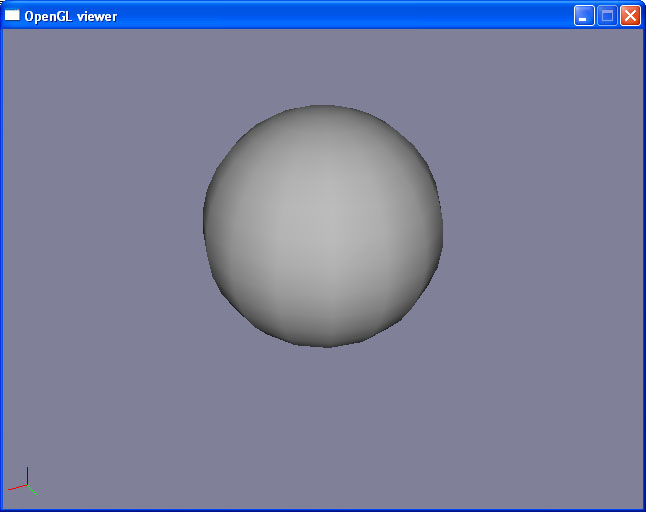
\includegraphics[width=8cm]{pics/helloworld}
\end{center}

The viewer tool reads the contents of the file which in this case
is an ordinary Python file and displays the scene using OpenGL.
When the input file is processed via the viewer tool it is executed
in a special environment where a couple of modules have already been imported.
That's why calling \code{Sphere()} doesn't result in a \exception{NameError}
exception. If you import the relevant modules yourself you can also call
the script without the viewer tool (however, you wouldn't get a visualization
of the scene then). You can also create the above scene directly in a 
Python shell:

\begin{verbatim}
>>> from cgkit.all import *
>>> Sphere()
<cgkit.quadrics.Sphere object at 0x051CC2D0>
\end{verbatim}

The first line imports all you need from cgkit which has to be done
manually now. The second line creates an instance of the
\class{Sphere} class. Usually, each object automatically inserts
itself into the scene, so we don't have to keep the resulting
reference. Now let's create another object:

\begin{verbatim}
>>> b=Box(name="Cube", pos=(1.5,2,0))
>>> listWorld()
Root
+---Cube (Box)
+---Sphere (Sphere)
\end{verbatim}

The first line creates a box object. This time we are passing a couple
of parameters like the object's name and its position and we store the
object in the variable \var{b} so we can manipulate the box afterwards.
The second line calls the \function{listWorld()} function
which prints a tree representation of the current scene.
Now it's time for a little nitpicking, actually the function only displays
the {\em world} (hence its name) and not the entire {\em scene}. The world
is what you see, it stores all 3D objects that have a visual representation
and is part of the scene. The whole scene also contains other objects
such as the timer, animation curves, etc. An object stored in the
scene is called a {\em component} and an object stored in the world
is, well, a {\em world object} (which is also a component as it is also
part of the scene). But back to the example. We have kept a reference to
the box, so let's see what we can do with it:

\begin{verbatim}
>>> b.name = "The Cube"
>>> listWorld()
Root
+---Sphere (Sphere)
+---The Cube (Box)
>>> b.pos
(1.5, 2, 0)
>>> b.pos=vec3(1,0,2)
>>> b.pos
(1, 0, 2)
>>> b.scale
(1, 1, 1)
\end{verbatim}

Every world object has a set of attributes that defines its state.
The exact set of attributes depends on the type of object, but there
are some common attributes that every world object has such as a name or
a position (see chapter \ref{worldobjects} for a reference of the available
world objects together with their attributes).

In the first example, we were only specifying one sphere with its default
attributes, that's why we had some geometry in the scene. But for a 3D scene
to be displayed you usually need two more ingredients: a camera and some 
light. In the above case, a default camera and light source was created
by the viewer tool. In the following example, we specify a complete scene,
including a camera, two colored light sources and a sphere with a material
assigned to it. Create a file "simplescene.py" with the following content:

\begin{verbatim}
TargetCamera(
    pos    = (3,2,2),
    target = (0,0,0)
)

GLPointLight(
    pos       = (3, -1, 2),
    diffuse   = (1, 0.7, 0.2)
)

GLPointLight(
    pos       = (-5, 3, 0),
    diffuse   = (0.2, 0.2, 0.5),
    intensity = 3.0
)

Sphere(
    name      = "My Sphere",
    radius    = 1.0,
    material  = GLMaterial(
                   diffuse = (0.7, 1, 0.7)
                )
)
\end{verbatim}

Display the scene by calling:

\begin{verbatim}
> viewer.py simplescene.py
\end{verbatim}

The result is this:

\begin{center}
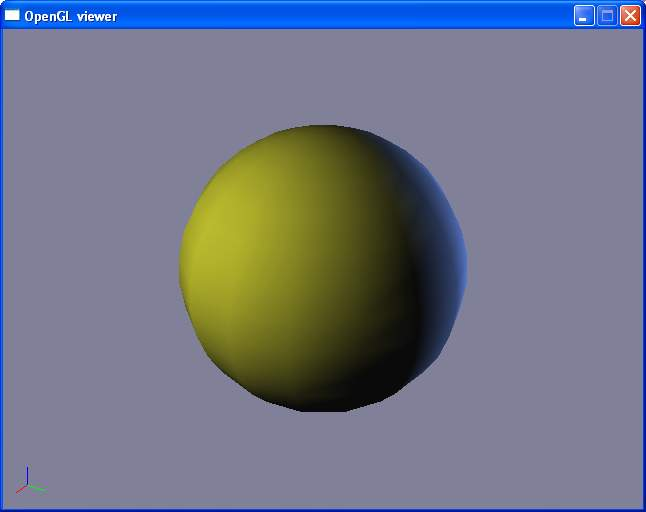
\includegraphics[width=8cm]{pics/simplescene1}
\end{center}

Using the \kbd{Alt} key in combination with the three mouse buttons
you can even navigate around in the scene (if you reach a pole
the camera position will jump around. This is because we are using
a \class{TargetCamera} that always tries to align its local "up"
direction with the global "up" direction, so this type of camera
can't be "upside down").

If you have a RenderMan renderer installed (there are free ones available
such as 3Delight, Aqsis or Pixie) you can try to visualize the above scene
with a different tool:

\begin{verbatim}
> render.py -r<renderer> simplescene.py
\end{verbatim}

\code{<renderer>} has to be replaced with either \code{3delight}, 
\code{aqsis} or \code{pixie}. 
This tool will display the same scene, but this time not using OpenGL but
the specified renderer. The result looks similar than before but is
much smoother:

\begin{center}
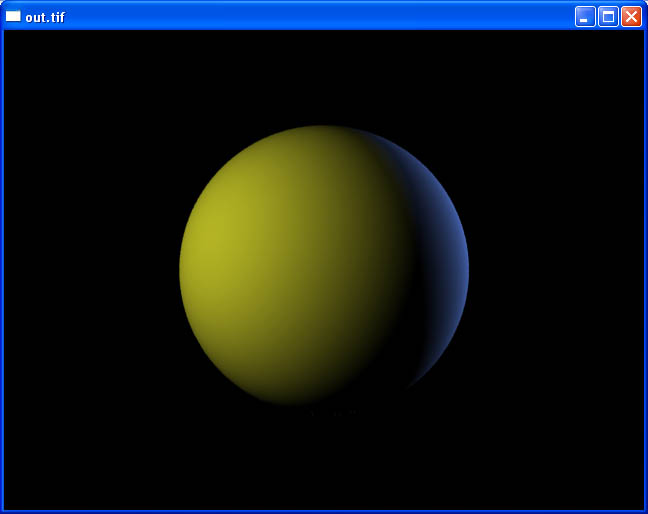
\includegraphics[width=8cm]{pics/simplescene2}
\end{center}

So if you want to create photorealistic images you can use the viewer tool
for previews and the render tool for creating the final image.

%----------------------------------------------------------------------
\section{Components and Slots}

This section gives an overview of the component framework that is the
basis for creating a dynamic 3D scene, i.e. one that is
animated/simulated. The basic mechanism is quite simple to understand
and you might already know it from other graphics packages as it is a
common concept in computer graphics software. The basic idea is to
have some black boxes that can generate values that vary with time and
that can be connected to the attributes we want to be animated. For
example, one such black box could output a three-dimensional vector
which could then be connected to the position of a teapot. If this
black box now produces a series of values that lie on a particular
curve we have an animation of a teapot traveling along that curve.

\begin{center}
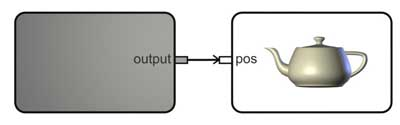
\includegraphics[width=10cm]{pics/slotexample}
\end{center}

In this package those black boxes and the teapot are called {\em
components}. A component is a container for {\em slots} which
represent the input or output values of their respective component. In
the above example, the output value of the "curve point generator" and
the position of the teapot are slots. You can also view them as
"animatable attributes" of an object if they mainly serve as input
values. Most slots can either serve as input value or output
value. However, if the value of a slot is actually computed by some
algorithm then this slot can only be used as output slot.

As a general rule, the actual slot corresponding to an attribute is
obtained by adding the suffix \code{_slot} to the attribute name.
Here is an example where two spheres s1 and s2 are created and
the position of s1 is connected to the position of s2 which means
s2 will always have the same position as s1:

\begin{verbatim}
>>> from cgkit import *
>>> s1=Sphere(pos=(1,2,3))
>>> s2=Sphere(pos=(-1,0,5))
>>> s1.pos
(1, 2, 3)
>>> s2.pos
(-1, 0, 5)

# Connect the positions 
>>> s1.pos_slot.connect(s2.pos_slot)

# Now s2 has the same position as s1
>>> s2.pos
(1, 2, 3)

# Changing the position of s1 will also change the position of s2
>>> s1.pos=vec3(-5,12,42)
>>> s2.pos
(-5, 12, 42)
\end{verbatim}

%----------------------------------------------------------------------
\section{Coordinate systems}

Each world object has a position and orientation in space. This
transformation can be described by a matrix that represents the
object's local coordinate system. The local coordinate system L stored
in each world object is given with respect to its parent coordinate
system which usually is just the world coordinate system unless you
have linked two objects. If you want the local coordinate system with
respect to the world system you have to travel up the transformation
hierarchy and concatenate all local systems (however, you don't have to
do that yourself as a world object already has an attribute 
\var{worldtransform} which does this for you). 

The geometry of a world object is given with respect to the local
coordinate system L. So this is the matrix that's required during
rendering. You get L by calling \method{localTransform()} on the
respective world object.

So far, if you would apply a rotation to an object it would rotate
around the origin or if you would scale the object the center of the
scale would lie in the origin. This is not always the desired behavior
and that's why you can specify a pivot point, or rather, a pivot
transformation or offset transformation P. This transformation is
given with respect to L and is the identity by default. You can get
and set this transformation using the \method{getOffsetTransform()} and
\method{setOffsetTransform()} methods.

The concatenation of L and P is the transformation T ($T=L\cdot
P$). This is what the
\var{transform}, \var{pos}, \var{rot} and \var{scale} slots of a world 
object describe. So if you modify the transform slot you also modify L
whereas P always remains constant, unless you change it explicitly via
\method{setOffsetTransform()}.

\begin{center}
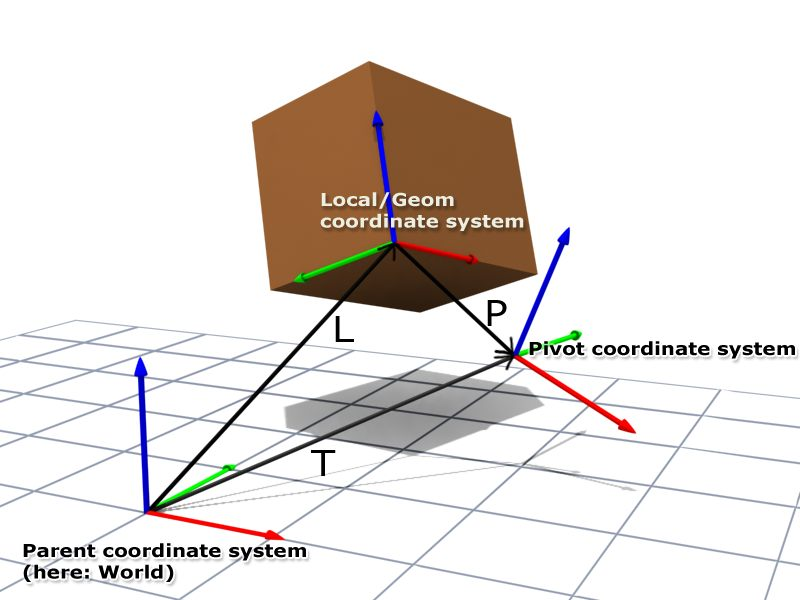
\includegraphics[width=12cm]{pics/coordsys}
\end{center}

Here is a simple code example where you can see the effects when
modifying the different transformations:

\begin{verbatim}
>>> s = Sphere()
>>> s.pos = vec3(1,2,0)
>>> s.pos
<1, 2, 0>
>>> s.setOffsetTransform(mat4().translation(vec3(2,4,7)))
>>> s.pos
<3, 6, 7>
>>> s.pos = vec3(0,0,0)
>>> s.pos
<0, 0, 0>
>>> s.localTransform()
[1, 0, 0, -2]
[0, 1, 0, -4]
[0, 0, 1, -7]
[0, 0, 0, 1]
\end{verbatim}

%---

\chapter{Building \& Installing \label{build}}

% Building and Installing

This chapter provides information about how to build the kit yourself
from the sources. You can skip this chapter if the kit is already
installed on your system or if you are installing binary versions.

%----------------------------------------------------------------------
\section{Building from the sources}

The following instructions will build and install the full version of cgkit.
You can also install the 'light' version by setting the variable 
\code{INSTALL_CGKIT_LIGHT} to \code{True} in your config file (just rename
the file \code{config_template.cfg} to \code{config.cfg} and uncomment the
corresponding line at the top of the file). Except for Python itself, 
installing the light version does not require any additional compiler, tool
or library, you simply have to call 

\begin{verbatim}
> python setup.py install    # that's all for the light version
\end{verbatim}

while being in the root directory of the cgkit sources. For installing
the light version you can skip the remainder of this section, but read
on if you actually want to install the full version.

The steps required to build the full version of the kit are the same
on every platform.  The build process assumes you have the following
tools/libraries installed on your system:

\begin{itemize}
\item \ulink{Boost}{http://www.boost.org/} (v1.31) - Make sure that Boost is
 installed including Boost.Python (e.g. Mac users who are using darwinports
 have to install the "+python" variant).
\item \ulink{SCons}{http://www.scons.org/} (v0.96.1)
\item \ulink{lib3ds}{http://lib3ds.sourceforge.net/} (v1.3.0) - {\bf Optional}. You need this if you want to import/export 3DS files.
\item \ulink{CyberX3D}{http://www.cybergarage.org/vrml/cx3d/cx3dcc/index.html} - {\bf Optional}. You need this if you want to import/export VRML or X3D files.
\item \ulink{OGRE}{http://www.ogre3d.org/} - {\bf Optional}. You need this if you want to use the OGRE-Viewer.
\item \ulink{STLport}{http://www.stlport.com/} - Only required on Windows when
 you want to use OGRE.
\item \ulink{3DxWare SDK}{http://www.3dconnexion.com/sdk.htm} - {\bf Optional} (currently Windows only). You need this if you want to use a SpaceMouse or SpaceBall.
\item \ulink{Wintab Programmer's Kit}{http://www.pointing.com/} - {\bf Optional} (Windows only). You need this if you want to use a tablet (or similar device).
\item \ulink{GloveSDK}{http://www.5dt.com/} - {\bf Optional}. You need this if you want to use a data glove. {\bf Note}: Download the version 2 SDK from the Ultra series, this can also be used with older gloves. You could also use version 1, but some functionality won't be available then.
\end{itemize}

If you have successfully installed the above tools and libraries you
can proceed with building the kit.The first step is to get the cgkit
sources. You can either download the source archive or check out the
latest version from CVS. The following build instructions apply to
both versions.

The package consists of three parts:

\begin{enumerate}
\item A pure C++ library that is independent of Python. This library is
 located in the \file{supportlib} directory.
\item Python wrappers around the above C++ library (using Boost.Python). 
 These wrappers are located in the \file{wrappers} directory.
\item The actual Python package using the wrappers. The package is located
 in the \file{cgkit} directory. The command line tools are in the main 
 directory.
\end{enumerate}

Part 2) and 3) is built and installed via the Python distutils (i.e.
the \file{setup.py} script). But before you can do so, you have to
build the C++ library manually using SCons.

{\bf Building the C++ support library:}

The C++ library is located in the directory \file{supportlib}. The library
uses SCons as its build system. If you have to customize the build process
you can create a file \file{cpp_config.cfg} where you can set some build
variables (e.g. adding search paths for include files). There is a template
file \file{cpp_config_template.cfg} which you can use to create the actual
config file. However, if you have installed every library in standard
directories it may well be that you don't need any config file at all.
Eventually you can build the library by calling \program{scons}:

\begin{verbatim}
> cd supportlib
> # ...create & modify cpp_config.cpp if necessary...
> scons
\end{verbatim}

If everything went fine you can see the result in the \file{lib}
subdirectory (\file{libcore.a} on Linux or \file{core.lib} on Windows).

{\bf Building the Python wrappers:}

The next step is to build and install the Python package. The package
uses the distutils, so you will find the familiar \file{setup.py}
script in the main directory. Customization of the build process can again
be done in a file called \file{config.cfg} which is executed by the setup
script. There is a template file \file{config_template.cfg} which you can
use to create your own config file. After setting up your
configuration you can install the package with the usual procedure:

\begin{verbatim}
> cd ..  # if you were still in the supportlib directory
> python setup.py install
\end{verbatim}

(see the manual \citetitle{Installing Python Modules} in your Python
documentation for more details about the distutils and how to proceed
if you have any special requirements)

Please also have a look at section \ref{externaldeps} for a list of
third-party packages you might have to install before you can use cgkit.
You can check cgkit and its dependencies with the script 
\file{utilities/checkenv.py} that is part of the source archive.
For a more thorough test you can run the unit tests in the \file{unittests}
directory.

A note to developers: You can build the package inplace by calling

\begin{verbatim}
> python setup.py build_ext --inplace
\end{verbatim}

In this case, the resulting binaries will be placed directly in the
\file{cgkit} directory which will then contain the entire package. Use
the \envvar{PYTHONPATH} variable and add the path to the main
directory if you want to use the inplace version from any other
directory.


%---

\chapter{Tools \label{tools}}

% Viewer tool

\section{The interactive viewer tool}

The tool \file{viewer.py} reads one or more files and displays the
scene using a simple OpenGL renderer. It creates events such as
keyboard, mouse or joystick events that can be used by the components
in the scene.

If the environment variable \envvar{VIEWER_DEFAULT_OPTIONS} exists, it
is read and parsed to set the default options. After that the options
in the command line are parsed.

{\bf Usage:}

\begin{verbatim}
viewer.py [options] inputfiles
\end{verbatim}

To exit the viewer press \kbd{Escape} or close the window. How to
navigate in the scene depends on the navigation mode (see option -N).

{\bf Options:}

\begin{description}
\item[\code{-f<int>} / \code{--fps=<int>}] 
Specifies the frame rate that should be tried to maintain while playing
back the scene (default: 30).

\item[\code{-h} / \code{--help}]
Print a help message.

\item[\code{-F} / \code{--full-screen}]
Open a full screen display.

\item[\code{-W<int>} / \code{--width=<int>}]
Specify the width in pixels of the window/screen (default: 640).

\item[\code{-H<int>} / \code{--height=<int>}]
Specify the height in pixels of the window/screen (default: 480). If
no height is specified it is computed based on the width and an aspect
ratio of 4/3.

\item[\code{-v} / \code{--verbose}]
Output info messages.

\item[\code{-p<str>} / \code{--plugin=<str>}]
If the argument specifies a file this file is loaded as a plugin, if it
is a directory, all files in this directory are loaded. You can specify
this option more than once or you can use a comma separated list of names.

You can also set files and paths via the environment variable
\envvar{CGKIT_PLUGIN_PATH}. The files/paths have to be separated either
by ':' or ';'.

\item[\code{-c<str>} / \code{--camera=<str>}]
Select the camera that should be used to view the scene. The argument
is the name of the camera. If no camera is specified the first camera
found in the scene is used.

\item[\code{-b<time>} / \code{--begin=<time>}]
Specify a time or frame where the animation/simulation should be started
(default: 0s). You can add the time unit such as 's' for seconds or 'f'
for frames. Frames are assumed if you don't specify a unit.

\item[\code{-e<time>} / \code{--end=<time>}]
Specify a time or frame where the animation/simulation should be stopped.
You can add the time unit such as 's' for seconds or 'f' for frames. 
Frames are assumed if you don't specify a unit.

\item[\code{-U<axis>} / \code{--up=<axis>}]
Specify the default value for the up axis. The argument may be either
'y' or 'z'.

\item[\code{-O<str>} / \code{--option=<str>}]
Add a global option that will be stored in the scene. The argument should
have the form "name=value". Using this option is equivalent to writing
"Globals( name=value )" in a scene file.

\item[\code{-t} / \code{--set-time}]
Set the starting time directly instead of stepping there from time 0.

\item[\code{-S<str>} / \code{--stereo=<str>}]
Activate stereo display. The argument specifies the method that should be
used to create a stereo image. It can be either \var{vsplit} or \var{glstereo}.

\item[\code{-D<float>} / \code{--eye-distance=<float>}]
Default eye distance for stereo display (default 0.07). This distance
value is used if the camera does not explicitly specify a distance value
(i.e. if it has no attribute \var{eye_distance}).

\item[\code{-B} / \code{--bounding-box}]
Display the bounding boxes.

\item[\code{-P<str>} / \code{--polygon-mode=<str>}]
Specify how polygons should be rendered. Possible values are
\var{fill} (default), \var{line} and \var{point}.

\item[\code{-s<str>} / \code{--save=<str>}]
When this option is specified each frame is saved under the given name
(+ frame number). The extension determines the image format.

\item[\code{-N<str>} / \code{--navigation-mode=<str>}]
Specify which navigation mode to activate. The viewer can emulate the
navigation of a few common 3D packages. Possible values are
\var{Maya} (default), \var{MAX} and \var{Softimage} (case-insensitive).

In Maya mode you navigate by pressing the \kbd{Alt} key in combination
with any of the three mouse buttons. In MAX mode you press the middle
mouse button either alone or in combination with \kbd{Alt} or \kbd{Control}
and \kbd{Alt}. In Softimage mode, only the Softimage Navigation Tool is
emulated (it's as if this tool is permanently active), i.e. you navigate
by using one of the three mouse buttons.

\item[\code{-X} / \code{--disable-spacedevice}]
Disables support for SpaceMouse/SpaceBall. This option can be used if there
are any problems with the driver or initialization takes too long.

\item[\code{-T} / \code{--disable-wintab}]
Disables tablet support. This option can be used if there are any
problems with the driver or initialization takes too long.

\end{description}

{\bf Events:}

The viewer tool generates the following user input events (see the
module \refmodule{cgkit.events} for more details about these events):

\begin{itemize}
\item \code{KEY_PRESS}
\item \code{KEY_RELEASE}
\item \code{LEFT_DOWN}
\item \code{MIDDLE_DOWN}
\item \code{RIGHT_DOWN}
\item \code{MOUSE_BUTTON_DOWN}
\item \code{LEFT_UP}
\item \code{MIDDLE_UP}
\item \code{RIGHT_UP}
\item \code{MOUSE_BUTTON_UP}
\item \code{MOUSE_WHEEL}
\item \code{MOUSE_MOVE}
\item \code{JOYSTICK_AXIS}
\item \code{JOYSTICK_BALL}
\item \code{JOYSTICK_HAT}
\item \code{JOYSTICK_BUTTON_DOWN}
\item \code{JOYSTICK_BUTTON_UP}
\item \code{SPACE_MOTION}
\item \code{SPACE_BUTTON_DOWN}
\item \code{SPACE_BUTTON_UP}
\item \code{SPACE_BUTTON_ZERO}
\item \code{TABLET}
\end{itemize}

{\bf Timing:}

The operations per frame are as follows (in this order):

\begin{enumerate}
\item Render and display the current scene at time $t$
\item Handle events
\item Step frame (i.e. increase the time by $\Delta t$ and signal the
  \code{STEP_FRAME} event)
\item Sync to the specified framerate
\end{enumerate}

% Render tool

\section{The render tool}

The tool \file{render.py} reads one or more files and renders the
scene using a RenderMan renderer. The tool takes care of creating the
RIB files and the shaders, compiling the shaders and launching the 
renderer.

If the environment variable \envvar{RENDER_DEFAULT_OPTIONS} exists, it
is read and parsed to set the default options. After that the options
in the command line are parsed.

{\bf Usage:}

\begin{verbatim}
render.py [options] inputfiles
\end{verbatim}


{\bf Options:}

\begin{description}
\item[\code{-f<int>} / \code{--fps=<int>}] 
Specifies the number of frames per second (default: 30).

\item[\code{-h} / \code{--help}]
Print a help message.

\item[\code{-W<int>} / \code{--width=<int>}]
Specify the width in pixels of the window/screen (default: 640).

\item[\code{-H<int>} / \code{--height=<int>}]
Specify the height in pixels of the window/screen (default: 480). If
no height is specified it is computed based on the width and an aspect
ratio of 4/3.

\item[\code{-v} / \code{--verbose}]
Output info messages.

\item[\code{-p<str>} / \code{--plugin=<str>}]
If the argument specifies a file this file is loaded as a plugin, if it
is a directory, all files in this directory are loaded. You can specify
this option more than once or you can use a comma separated list of names.

You can also set files and paths via the environment variable
\envvar{CGKIT_PLUGIN_PATH}. The files/paths have to be separated either
by ':' or ';'.

\item[\code{-c<str>} / \code{--camera=<str>}]
Select the camera that should be used to view the scene. The argument
is the name of the camera. If no camera is specified the first camera
found in the scene is used.

\item[\code{-b<time>} / \code{--begin=<time>}]
Specify a time or frame where the animation/simulation should be started
(default: 0s). You can add the time unit such as 's' for seconds or 'f'
for frames. Frames are assumed if you don't specify a unit.

\item[\code{-e<time>} / \code{--end=<time>}]
Specify a time or frame where the animation/simulation should be stopped.
You can add the time unit such as 's' for seconds or 'f' for frames. 
Frames are assumed if you don't specify a unit.

\item[\code{-U<axis>} / \code{--up=<axis>}]
Specify the default value for the up axis. The argument may be either
'y' or 'z'.

\item[\code{-O<str>} / \code{--option=<str>}]
Add a global option that will be stored in the scene. The argument should
have the form "name=value". Using this option is equivalent to writing
"Globals( name=value )" in a scene file.

\item[\code{-t} / \code{--set-time}]
Set the starting time directly instead of stepping there from time 0.

\item[\code{-r<str>} / \code{--renderer=<str>}]
Select the renderer to use (you can choose among \code{aqsis},
\code{3delight}, \code{pixie}, \code{prman}, \code{air} and \code{rdc}).

\item[\code{-I<str>} / \code{--include=<str>}]
Add the specified include path to the list of paths used for compiling
the shaders.

\item[\code{-B} / \code{--bake}]
Activate texture baking mode.

\end{description}

{\bf Events:}

The render tool does not generate any user input events.


%---

\chapter{Generic modules \label{modules1}}

\localmoduletable

\section{\module{cgkitinfo} ---
         Release information}

\declaremodule{extension}{cgkit.cgkitinfo}
\modulesynopsis{Provides version information.}

New in version 1.1. This module contains two variables that carry
information about the version of the kit.

\begin{datadesc}{version}
A string containing version information of this release.
\end{datadesc}

\begin{datadesc}{version_info}
A 4-tuple (\var{major}, \var{minor}, \var{micro}, \var{releaselevel})
containing the components of the version number. The first three
values are integers, whereas \var{releaselevel} is a string containing
"cvs", "alpha", "beta" or "final".
\end{datadesc}

\section{\module{cgtypes} ---
         Vectors, matrices and quaternions}

\declaremodule{extension}{cgkit.cgtypes}
\modulesynopsis{Basic types useful for computer graphics.}

This module contains the fundamental types which make working with 3D
data much easier. The types are:

\begin{itemize}
\item vec3 -- a three dimensional vector type to store points, vectors, normals or even colors.
\item vec4 -- a four dimensional vector type to store homogenous points, for example.
\item mat3 -- a 3x3 matrix to store linear transformations.
\item mat4 -- a 4x4 matrix to store affine transformations.
\item quat -- a quaternion type as a specialized way to store rotations.
\end{itemize}

You import all of those types at once with

\begin{verbatim}
from cgkit.cgtypes import *
\end{verbatim}

or you can import them individually like this

\begin{verbatim}
from cgkit.cgtypes import vec3, mat4
\end{verbatim}

In general, you can use those types just as if they were built-in
types which means the mathematical operators can be used and have
their respective meaning. Each type has some additional methods which
are described in the respective documentation.

Here are some examples:

\begin{verbatim}
>>> from cgkit.cgtypes import *
>>> v=vec3(0.5,1.0,-2.5)
>>> print v
(0.5000, 1.0000, -2.5000)
>>> print v.length()
2.73861278753
>>> v=v.normalize()
>>> print v
(0.1826, 0.3651, -0.9129)
>>> print v.length()
1.0
\end{verbatim}

Now let's construct a rotation matrix that rotates points by 90
degrees around the z-axis:

\begin{verbatim}
>>> M=mat4(1).rotate(0.5*math.pi, vec3(0,0,1))
\end{verbatim}

and apply the rotation to the vector (1,0,0) (the x-axis):

\begin{verbatim}
>>> print M*vec3(1,0,0)
(0.0000, 1.0000, 0.0000)
\end{verbatim}

The module contains the following functions:

\begin{funcdesc}{getEpsilon}{}
Return the epsilon threshold which is used for doing comparisons.
\end{funcdesc}

\begin{funcdesc}{setEpsilon}{eps}
Sets a new epsilon threshold and returns the previously set value. Two
values are considered to be equal if their absolute difference is less
than or equal to epsilon.
\end{funcdesc}

\begin{funcdesc}{slerp}{t, q0, q1}
Performs a spherical linear interpolation between two quaternions q0
and q1. For t=0.0 the return value equals q0, for t=1.0 it equals
q1. q0 and q1 must be unit quaternions. \\
New in version 1.1.
\end{funcdesc}

\begin{funcdesc}{squad}{t, a, b, c, d}
Performs a spherical cubic interpolation between quaternion a and d
where quaternion b and c define the shape of the interpolation
curve. For t=0.0 the return value equals a, for t=1.0 it equals d. All
quaternions must be unit quaternions. \\
New in version 1.1.
\end{funcdesc}

%----------------------------------------------------------------------
\subsection{vec3 - 3d vector}
\label{vec3}

A \class{vec3} represents a 3D vector type that can be used to store
points, vector, normals or even colors. You can construct a
\class{vec3} by several ways:

\begin{verbatim}
# all components are set to zero
v = vec3()

-> (0.0000, 0.0000, 0.0000)

# set all components to one value
v = vec3(2.5)

-> (2.5000, 2.5000, 2.5000)

# set a 2d vector, the 3rd component will be zero
v = vec3(1.5, 0.8)

-> (1.5000, 0.8000, 0.0000)

# initialize all three components
v = vec3(1.5, 0.8, -0.5)

-> (1.5000, 0.8000, -0.5000)
\end{verbatim}

Additionally you can use all of the above, but store the values inside
a tuple, a list or a string:

\begin{verbatim}
v = vec3([1.5, 0.8, -0.5])
w = vec3("1.5, 0.8")
\end{verbatim}

Finally, you can initialize a vector with a copy of another vector:

\begin{verbatim}
v = vec3(w)
\end{verbatim}

A \class{vec3} can be used just like a list with 3 elements, so you
can read and write components using the index operator or by accessing
the components by name:

\begin{verbatim}
>>> v=vec3(1,2,3)
>>> print v[0]
1.0
>>> print v.y
2.0
\end{verbatim}

%----------------------------------------
{\bf Mathematical operations}

The mathematical operators are supported with the following
combination of types:

\begin{verbatim}
vec3  =  vec3 + vec3
vec3  =  vec3 - vec3
float =  vec3 * vec3      # dot product
vec3  = float * vec3
vec3  =  vec3 * float
vec3  =  vec3 / float
vec3  =  vec3 % float     # each component
vec3  =  vec3 % vec3      # component wise
vec3  = -vec3
float =  vec3[i]          # get or set element
\end{verbatim}

Additionally, you can compare vectors with \code{==}, \code{!=}, \code{<}, 
\code{<=}, \code{>}, \code{>=}. Each
comparison (except \code{<} and \code{>}) takes an epsilon environment
into account, this means two values are considered to be equal if
their absolute difference is less than or equal to a threshold value
epsilon. You can read and write this threshold value using the
functions \function{getEpsilon()} and \function{setEpsilon()}.

Taking the absolute value of a vector will return the length of the vector: 

\begin{verbatim}
float = abs(v)            # this is equivalent to v.length()
\end{verbatim}

%----------------------------------------
{\bf Methods}

\begin{methoddesc}{angle}{other}
Return angle (in radians) between \var{self} and \var{other}.
\end{methoddesc}

\begin{methoddesc}{cross}{other}
Return cross product of \var{self} and \var{other}.
\end{methoddesc}

\begin{methoddesc}{length}{}
Returns the length of the vector ($\sqrt{x^2+y^2+z^2}$). This is
equivalent to calling \code{abs(self)}.
\end{methoddesc}

\begin{methoddesc}{normalize}{}
Returns normalized vector. If the method is called on the null vector
(where each component is zero) a \exception{ZeroDivisionError} is raised.
\end{methoddesc}

\begin{methoddesc}{reflect}{N}
Returns the reflection vector. \var{N} is the surface normal which has to be
of unit length.
\end{methoddesc}

\begin{methoddesc}{refract}{N, eta}
Returns the transmitted vector. \var{N} is the surface normal which has to
be of unit length. \var{eta} is the relative index of refraction. If the
returned vector is zero then there is no transmitted light because of
total internal reflection.
\end{methoddesc}

\begin{methoddesc}{ortho}{}
Returns a vector that is orthogonal to \var{self} (where
\code{self*self.ortho()==0}).
\end{methoddesc}

\begin{methoddesc}{min}{}
Returns the minimum value of the components.
\end{methoddesc}

\begin{methoddesc}{max}{}
Returns the maximum value of the components.
\end{methoddesc}

\begin{methoddesc}{minIndex}{}
Return the index of the component with the minimum value.
\end{methoddesc}

\begin{methoddesc}{maxIndex}{}
Return the index of the component with the maximum value.
\end{methoddesc}

\begin{methoddesc}{minAbs}{}
Returns the minimum absolute value of the components.
\end{methoddesc}

\begin{methoddesc}{maxAbs}{}
Returns the maximum absolute value of the components.
\end{methoddesc}

\begin{methoddesc}{minAbsIndex}{}
Return the index of the component with the minimum absolute value.
\end{methoddesc}

\begin{methoddesc}{maxAbsIndex}{}
Return the index of the component with the maximum absolute value.
\end{methoddesc}


%----------------------------------------------------------------------
\subsection{vec4 - 4d vector}
\label{vec4}

A \class{vec4} represents a 4D vector type. You can construct a \class{vec4}
by several ways:

\begin{verbatim}
# all components are set to zero
v = vec4()

-> (0.0000, 0.0000, 0.0000, 0.0000)

# set all components to one value
v = vec4(2.5)

-> (2.5000, 2.5000, 2.5000, 2.5000)

# set a 2d vector, the ramaining components will be zero
v = vec4(1.5, 0.8)

-> (1.5000, 0.8000, 0.0000, 0.0000)

# set a 3d vector, the ramaining component will be zero
v = vec4(1.5, 0.8, -0.5)

-> (1.5000, 0.8000, -0.5000, 0.0000)

# set all components
v = vec4(1.5, 0.8, -0.5, 0.2)

-> (1.5000, 0.8000, -0.5000, 0.2000)
\end{verbatim}

Additionally you can use all of the above, but store the values inside
a tuple, a list or a string:

\begin{verbatim}
v = vec4([1.5, 0.8, -0.5])
w = vec4("1.5, 0.8")
\end{verbatim}

Finally, you can initialize a vector with a copy of another vector:

\begin{verbatim}
v = vec4(w)
\end{verbatim}

A \class{vec4} can be used just like a list with 4 elements, so you
can read and write components using the index operator or by accessing
the components by name:

\begin{verbatim}
>>> v=vec4(1,2,3,1)
>>> print v[0]
1.0
>>> print v.y
2.0
>>> print v.w
1.0
>>> print v.t   # this is the same as v.w
1.0
\end{verbatim}

The 4th component can be accessed either by the name \code{w} or
\code{t}. You might prefer the former name when using the vector as a
homogenous coordinate while the latter might be preferable when the
4th component shall represent a time value.

%----------------------------------------
{\bf Mathematical operations}

The mathematical operators are supported with the following
combination of types:

\begin{verbatim}
vec4  =  vec4 + vec4
vec4  =  vec4 - vec4
float =  vec4 * vec4      # dot product
vec4  = float * vec4
vec4  =  vec4 * float
vec4  =  vec4 / float
vec4  =  vec4 % float     # each component
vec4  =  vec4 % vec4      # component wise
vec4  = -vec4
float =  vec4[i]          # get or set element
\end{verbatim}

Additionally, you can compare vectors with \code{==}, \code{!=}, \code{<}, 
\code{<=}, \code{>}, \code{>=}. Each
comparison (except \code{<} and \code{>}) takes an epsilon environment
into account, this means two values are considered to be equal if
their absolute difference is less than or equal to a threshold value
epsilon. You can read and write this threshold value using the
functions \function{getEpsilon()} and \function{setEpsilon()}.

Taking the absolute value of a vector will return the length of the vector: 

\begin{verbatim}
float = abs(v)            # this is equivalent to v.length()
\end{verbatim}

%----------------------------------------
{\bf Methods}

\begin{methoddesc}{length}{}
Returns the length of the vector ($\sqrt{x^2+y^2+z^2}$). This is
equivalent to calling \code{abs(self)}.
\end{methoddesc}

\begin{methoddesc}{normalize}{}
Returns normalized vector. If the method is called on the null vector
(where each component is zero) a \exception{ZeroDivisionError} is raised.
\end{methoddesc}




%----------------------------------------------------------------------
\subsection{mat3 - 3x3 matrix}
\label{mat3}

A \class{mat3} represents a 3x3 matrix which can be used to store
linear transformations (if you want to store translations or
perspective transformations, you have to use a \class{mat4}). You can
construct a \class{mat3} in several ways:

\begin{verbatim}
# all components are set to zero
M = mat3()

[   0.0000,    0.0000,    0.0000]
[   0.0000,    0.0000,    0.0000]
[   0.0000,    0.0000,    0.0000]

# identity matrix
M = mat3(1.0)

[   1.0000,    0.0000,    0.0000]
[   0.0000,    1.0000,    0.0000]
[   0.0000,    0.0000,    1.0000]

# The elements on the diagonal are set to 2.5
M = mat3(2.5)

[   2.5000,    0.0000,    0.0000]
[   0.0000,    2.5000,    0.0000]
[   0.0000,    0.0000,    2.5000]

# All elements are explicitly set (values must be given in row-major order)
M = mat3(a,b,c,d,e,f,g,h,i)
M = mat3([a,b,c,d,e,f,g,h,i])

[ a, b, c]
[ d, e, f]
[ g, h, i]

# Create a copy of matrix N (which also has to be a mat3)
M = mat3(N)

# Specify the 3 columns of the matrix (as vec3's or sequences with 3 elements)
M = mat3(a,b,c)

[ a[0], b[0], c[0] ]
[ a[1], b[1], c[1] ]
[ a[2], b[2], c[2] ]

# All elements are explicitly set and are stored inside a string
M = mat3("1,2,3,4,5,6,7,8,9")

[   1.0000,    2.0000,    3.0000]
[   4.0000,    5.0000,    6.0000]
[   7.0000,    8.0000,    9.0000]
\end{verbatim}

%----------------------------------------
{\bf Mathematical operations}

The mathematical operators are supported with the following
combination of types:

\begin{verbatim}
mat3  =  mat3 + mat3
mat3  =  mat3 - mat3
mat3  =  mat3 * mat3
vec3  =  mat3 * vec3
vec3  =  vec3 * mat3
mat3  = float * mat3
mat3  =  mat3 * float
mat3  =  mat3 / float
mat3  =  mat3 % float     # each component
mat3  = -mat3
vec3  =  mat3[i]          # get or set column i (as vec3)
float =  mat3[i,j]        # get or set element in row i and column j
\end{verbatim}

Additionally, you can compare matrices with \code{==} and \code{!=}.

%----------------------------------------
{\bf Methods}

\begin{methoddesc}{getColumn}{index}
Return column index (0-based) as a \class{vec3}.
\end{methoddesc}

\begin{methoddesc}{setColumn}{index, value}
Set column index (0-based) to \var{value} which has to be a sequence
of 3 floats (this includes \class{vec3}).
\end{methoddesc}

\begin{methoddesc}{getRow}{index}
Return row index (0-based) as a \class{vec3}.
\end{methoddesc}

\begin{methoddesc}{setRow}{index, value}
Set row index (0-based) to \var{value} which has to be a sequence of
3 floats (this includes \class{vec3}).
\end{methoddesc}

\begin{methoddesc}{getDiag}{}
Return the diagonal as a \class{vec3}.
\end{methoddesc}

\begin{methoddesc}{setDiag}{value}
Set the diagonal to \var{value} which has to be a sequence of
3 floats (this includes \class{vec3}).
\end{methoddesc}

\begin{methoddesc}{toList}{rowmajor=False}
Returns a list containing the matrix elements. By default, the list is
in column-major order. If you set the optional argument \var{rowmajor} to
\code{True}, you'll get the list in row-major order.
\end{methoddesc}

\begin{methoddesc}{identity}{}
Returns the identity matrix. 
\end{methoddesc}

\begin{methoddesc}{transpose}{}
Returns the transpose of the matrix.
\end{methoddesc}

\begin{methoddesc}{determinant}{}
Returns the determinant of the matrix.
\end{methoddesc}

\begin{methoddesc}{inverse}{}
Returns the inverse of the matrix.
\end{methoddesc}

\begin{methoddesc}{scaling}{s}
Returns a scaling transformation. The scaling vector \var{s} must be a
3-sequence (e.g. a \class{vec3}).

\[ \left( \begin{array}{ccc}
s.x & 0 & 0 \\
0 & s.y & 0 \\
0 & 0 & s.z \\
\end{array} \right) \]
\end{methoddesc}

\begin{methoddesc}{rotation}{angle, axis}
Returns a rotation transformation. The angle must be given in radians,
\var{axis} has to be a 3-sequence (e.g. a \class{vec3}).
\end{methoddesc}

\begin{methoddesc}{scale}{s}
Concatenates a scaling transformation and returns \var{self}. The scaling
vector s must be a 3-sequence (e.g. a \class{vec3}).
\end{methoddesc}

\begin{methoddesc}{rotate}{angle, axis}
Concatenates a rotation transformation and returns \var{self}. The angle
must be given in radians, axis has to be a 3-sequence (e.g. a \class{vec3}).
\end{methoddesc}

\begin{methoddesc}{ortho}{}
Returns a matrix with orthogonal base vectors.
\end{methoddesc}

\begin{methoddesc}{decompose}{}
Decomposes the matrix into a rotation and scaling part. The method
returns a tuple (rotation, scaling). The scaling part is given as a
\class{vec3}, the rotation is still a \class{mat3}.
\end{methoddesc}

\begin{methoddesc}{fromEulerXYZ}{x, y, z}
Initializes a rotation matrix from Euler angles. \var{x} is the angle
around the x axis, \var{y} the angle around the y axis and \var{z} the
angle around the z axis. All angles must be given in radians. The order
of the individual rotations is X-Y-Z (where each axis refers to the {\em
local} axis, i.e. the first rotation is about the x axis which rotates
the Y and Z axis, then the second rotation is about the rotated Y axis 
and so on).
\end{methoddesc}

\begin{methoddesc}{fromEulerYZX}{x, y, z}
See above. The order is YZX.
\end{methoddesc}

\begin{methoddesc}{fromEulerZXY}{x, y, z}
See above. The order is ZXY.
\end{methoddesc}

\begin{methoddesc}{fromEulerXZY}{x, y, z}
See above. The order is XZY.
\end{methoddesc}

\begin{methoddesc}{fromEulerYXZ}{x, y, z}
See above. The order is YXZ.
\end{methoddesc}

\begin{methoddesc}{fromEulerZYX}{x, y, z}
See above. The order is ZYX.
\end{methoddesc}

\begin{methoddesc}{toEulerXYZ}{}
Return the Euler angles of a rotation matrix. The order is XYZ.
\end{methoddesc}

\begin{methoddesc}{toEulerYZX}{}
Return the Euler angles of a rotation matrix. The order is YZX.
\end{methoddesc}

\begin{methoddesc}{toEulerZXY}{}
Return the Euler angles of a rotation matrix. The order is ZXY.
\end{methoddesc}

\begin{methoddesc}{toEulerXZY}{}
Return the Euler angles of a rotation matrix. The order is XZY.
\end{methoddesc}

\begin{methoddesc}{toEulerYXZ}{}
Return the Euler angles of a rotation matrix. The order is YXZ.
\end{methoddesc}

\begin{methoddesc}{toEulerZYX}{}
Return the Euler angles of a rotation matrix. The order is ZYX.
\end{methoddesc}


%----------------------------------------------------------------------
\subsection{mat4 - 4x4 matrix}
\label{mat4}

A \class{mat4} represents a 4x4 matrix which can be used to store
transformations. You can construct a \class{mat4} in several ways:

\begin{verbatim}
# all components are set to zero
M = mat4()

[   0.0000,    0.0000,    0.0000,    0.0000]
[   0.0000,    0.0000,    0.0000,    0.0000]
[   0.0000,    0.0000,    0.0000,    0.0000]
[   0.0000,    0.0000,    0.0000,    0.0000]

# identity matrix
M = mat4(1.0)

[   1.0000,    0.0000,    0.0000,    0.0000]
[   0.0000,    1.0000,    0.0000,    0.0000]
[   0.0000,    0.0000,    1.0000,    0.0000]
[   0.0000,    0.0000,    0.0000,    1.0000]

# The elements on the diagonal are set to 2.5
M = mat4(2.5)

[   2.5000,    0.0000,    0.0000,    0.0000]
[   0.0000,    2.5000,    0.0000,    0.0000]
[   0.0000,    0.0000,    2.5000,    0.0000]
[   0.0000,    0.0000,    0.0000,    2.5000]

# All elements are explicitly set (values must be given in row-major order)
M = mat4(a,b,c,d,e,f,g,h,i,j,k,l,m,n,o,p)
M = mat4([a,b,c,d,e,f,g,h,i,j,k,l,m,n,o,p])

[ a, b, c, d ]
[ e, f, g, h ]
[ i, j, k, l ]
[ m, n, o, p ]

# Create a copy of matrix N (which also has to be a mat4)
M = mat4(N)

# Specify the 4 columns of the matrix (as vec4's or sequences with 4 elements)
M = mat4(a,b,c,d)

[ a[0], b[0], c[0], d[0] ]
[ a[1], b[1], c[1], d[1] ]
[ a[2], b[2], c[2], d[2] ]
[ a[3], b[3], c[3], d[3] ]

# All elements are explicitly set and are stored inside a string
M = mat4("1,2,3,4,5,6,7,8,9,10,11,12,13,14,15,16")

[   1.0000,    2.0000,    3.0000,    4.0000]
[   5.0000,    6.0000,    7.0000,    8.0000]
[   9.0000,   10.0000,   11.0000,   12.0000]
[  13.0000,   14.0000,   15.0000,   16.0000]
\end{verbatim}

%----------------------------------------
{\bf Mathematical operations}

The mathematical operators are supported with the following
combination of types:

\begin{verbatim}
mat4  =  mat4 + mat4
mat4  =  mat4 - mat4
mat4  =  mat4 * mat4
vec4  =  mat4 * vec4
vec4  =  vec4 * mat4
vec3  =  mat4 * vec3      # missing coordinate in vec3 is implicitly set to 1.0
vec3  =  vec3 * mat4      # missing coordinate in vec3 is implicitly set to 1.0
mat4  = float * mat4
mat4  =  mat4 * float
mat4  =  mat4 / float
mat4  =  mat4 % float     # each component
mat4  = -mat4
vec4  =  mat4[i]          # get or set column i (as vec4)
float =  mat4[i,j]        # get or set element in row i and column j
\end{verbatim}

Additionally, you can compare matrices with \code{==} and \code{!=}.

%----------------------------------------
{\bf Methods}

\begin{methoddesc}{getColumn}{index}
Return column index (0-based) as a \class{vec4}.
\end{methoddesc}

\begin{methoddesc}{setColumn}{index, value}
Set column index (0-based) to \var{value} which has to be a sequence
of 4 floats (this includes \class{vec4}).
\end{methoddesc}

\begin{methoddesc}{getRow}{index}
Return row index (0-based) as a \class{vec4}.
\end{methoddesc}

\begin{methoddesc}{setRow}{index, value}
Set row index (0-based) to \var{value} which has to be a sequence of
4 floats (this includes \class{vec4}).
\end{methoddesc}

\begin{methoddesc}{getDiag}{}
Return the diagonal as a \class{vec4}.
\end{methoddesc}

\begin{methoddesc}{setDiag}{value}
Set the diagonal to \var{value} which has to be a sequence of
4 floats (this includes \class{vec4}).
\end{methoddesc}

\begin{methoddesc}{toList}{rowmajor=False}
Returns a list containing the matrix elements. By default, the list is
in column-major order (which can be directly used in OpenGL or RenderMan). 
If you set the optional argument \var{rowmajor} to
\code{True}, you will get the list in row-major order.
\end{methoddesc}

\begin{methoddesc}{identity}{}
Returns the identity matrix. 
\end{methoddesc}

\begin{methoddesc}{transpose}{}
Returns the transpose of the matrix.
\end{methoddesc}

\begin{methoddesc}{determinant}{}
Returns the determinant of the matrix.
\end{methoddesc}

\begin{methoddesc}{inverse}{}
Returns the inverse of the matrix.
\end{methoddesc}

\begin{methoddesc}{translation}{t}
Returns a translation transformation. The translation vector t must be a
3-sequence (e.g. a vec3).

\[ \left( \begin{array}{cccc}
1 & 0 & 0 & t.x \\
0 & 1 & 0 & t.x \\
0 & 0 & 1 & t.x \\
0 & 0 & 0 & 1 
\end{array} \right) \]

\end{methoddesc}

\begin{methoddesc}{scaling}{s}
Returns a scaling transformation. The scaling vector \var{s} must be a
3-sequence (e.g. a \class{vec3}).

\[ \left( \begin{array}{cccc}
s.x & 0 & 0 & 0\\
0 & s.y & 0 & 0\\
0 & 0 & s.z & 0\\
0 & 0 & 0 & 1\\
\end{array} \right) \]
\end{methoddesc}

\begin{methoddesc}{rotation}{angle, axis}
Returns a rotation transformation. The angle must be given in radians,
\var{axis} has to be a 3-sequence (e.g. a \class{vec3}).
\end{methoddesc}

\begin{methoddesc}{translate}{t}
Concatenate a translation transformation and return \var{self}. The
translation vector \var{t} must be a 3-sequence (e.g. a \class{vec3}).
\end{methoddesc}

\begin{methoddesc}{scale}{s}
Concatenates a scaling transformation and returns \var{self}. The scaling
vector s must be a 3-sequence (e.g. a \class{vec3}).
\end{methoddesc}

\begin{methoddesc}{rotate}{angle, axis}
Concatenates a rotation transformation and returns \var{self}. The angle
must be given in radians, axis has to be a 3-sequence (e.g. a \class{vec3}).
\end{methoddesc}

\begin{methoddesc}{frustum}{left, right, bottom, top, near, far}
Returns a matrix that represents a perspective depth
transformation. This method is equivalent to the OpenGL command
\cfunction{glFrustum()}.

\note{If you want to use this transformation in RenderMan, keep in
mind that the RenderMan camera is looking in the positive z direction
whereas the OpenGL camera is looking in the negative direction.}
\end{methoddesc}

\begin{methoddesc}{perspective}{fovy, aspect, near, far}
Similarly to \method{frustum()} this method returns a perspective
transformation, the only difference is the meaning of the input
parameters. The method is equivalent to the OpenGL command
\cfunction{gluPerspective()}.
\end{methoddesc}

\begin{methoddesc}{orthographic}{left, right, bottom, top, near, far}
Returns a matrix that represents an orthographic transformation. This
method is equivalent to the OpenGL command \cfunction{glOrtho()}.
\end{methoddesc}

\begin{methoddesc}{lookAt}{pos, target, up=(0,0,1)}
Returns a transformation that moves the coordinate system to position
\var{pos} and rotates it so that the z-axis points onto point
\var{target}. The y-axis is pointing as closely as possible into the
same direction as \var{up}. All three parameters have to be a
3-sequence.

You can use this transformation to position objects in the scene that
have to be oriented towards a particular point. Or you can use it to
position the camera in the virtual world. In this case you have to
take the inverse of this transformation as viewport transformation (to
convert world space coordinates into camera space coordinates).
\end{methoddesc}

\begin{methoddesc}{ortho}{}
Returns a matrix with orthogonal base vectors. The x-, y- and z-axis
are made orthogonal. The fourth column and row remain untouched.
\end{methoddesc}

\begin{methoddesc}{decompose}{}
Decomposes the matrix into a translation, rotation and scaling. The
method returns a tuple (translation, rotation, scaling). The
translation and scaling parts are given as \class{vec3}, the rotation is
still given as a \class{mat4}.
\end{methoddesc}

\begin{methoddesc}{getMat3}{}
Returns a \class{mat3} which is a copy of self without the 4th column and row.
\end{methoddesc}

\begin{methoddesc}{setMat3}{m3}
Sets the first three columns and rows to the values in \var{m3}.
\end{methoddesc}




%----------------------------------------------------------------------
\subsection{quat - quaternions}
\label{quat}

A \class{quat} represents a quaternion type that can be used to store
rotations. A quaternion contains four values of which one can be seen
as the angle and the other three as the axis of rotation. The most
common way to initialize a quaternion is by specifying an angle (in
radians) and the axis of rotation:

\begin{verbatim}
# initialize the quaternion by specifying an angle and the axis of rotation
q = quat(0.5*pi, vec3(0,0,1))

# initialize by specifying a rotation matrix (as mat3 or mat4)
q = quat(R)

# all components are set to zero
q = quat()

(0.0000, 0.0000, 0.0000, 0.0000)

# set the w component
q = quat(2.5)

(0.5000, 0.0000, 0.0000, 0.0000)

# set all four components (w,x,y,z)
q = quat(1,0,0,0)
q = quat([1,0,0,0])
q = quat("1,0,0,0")

(1.0000, 0.0000, 0.0000, 0.0000)
\end{verbatim}

Finally, you can initialize a quaternion with a copy of another quaternion:

\begin{verbatim}
q = quat(r)
\end{verbatim}

%----------------------------------------
{\bf Mathematical operations}

The mathematical operators are supported with the following
combination of types:

\begin{verbatim}
quat  =  quat + quat
quat  =  quat - quat
quat  =  quat * quat
quat  = float * quat
quat  =  quat * float
quat  =  quat / float
quat  = -quat
quat  =  quat ** float = pow(quat, float)   (new in version 1.1)
quat  =  quat ** quat  = pow(quat, quat)    (new in version 1.1)
\end{verbatim}

Additionally, you can compare quaternions with \code{==} and \code{!=}. 
Taking the absolute value will return the magnitude of the quaternion:

\begin{verbatim}
float = abs(q)
\end{verbatim}

%----------------------------------------
{\bf Methods}

\begin{methoddesc}{conjugate}{}
Return the conjugate $(w, -x, -y, -z)$ of the quaternion.
\end{methoddesc}

\begin{methoddesc}{normalize}{}
Returns the normalized quaternion. If the method is called on the null
vector a \exception{ZeroDivisionError} is raised.
\end{methoddesc}

\begin{methoddesc}{inverse}{}
Return the inverse of the quaternion.
\end{methoddesc}

\begin{methoddesc}{toAngleAxis}{}
Returns a tuple containing the angle (in radians) and the axis of rotation.
The returned axis can also be zero if the rotation is actually the identity.
\end{methoddesc}

\begin{methoddesc}{fromAngleAxis}{angle, axis}
Initializes \var{self} from an angle (in radians) and an axis of
rotation and returns \var{self}. The initialized quaternion will be a
unit quaternion. Passing the null vector as axis has the same effect
as passing an angle of 0 (i.e. the quaternion will be set to (1,0,0,0)).
\end{methoddesc}

\begin{methoddesc}{toMat3}{}
Convert the quaternion into a rotation matrix and return the matrix as a 
\class{mat3}.
\end{methoddesc}

\begin{methoddesc}{toMat4}{}
Convert the quaternion into a rotation matrix and return the matrix as a 
\class{mat4}.
\end{methoddesc}

\begin{methoddesc}{fromMat}{matrix}
Initialize \var{self} from a rotation matrix, given either as a
\class{mat3} or a \class{mat4} and returns \var{self}. \var{matrix} must be
a rotation matrix (i.e. the determinant is 1), if you have a matrix
that is made up of other parts as well, call \method{matrix.decompose()} to get
the rotation part.
\end{methoddesc}

\begin{methoddesc}{dot}{b}
Returns the dot product of \var{self} with quaternion \var{b}.\\
New in version 1.1.
\end{methoddesc}

\begin{methoddesc}{log}{}
Returns the natural logarithm of \var{self}.\\
New in version 1.1.
\end{methoddesc}

\begin{methoddesc}{exp}{}
Returns the exponential of \var{self}. \\
New in version 1.1.
\end{methoddesc}

%----------------------------------------
{\bf Related functions}

\begin{funcdesc}{slerp}{t, q0, q1, shortest=True}
Performs a spherical linear interpolation between two quaternions \var{q0}
and \var{q1}. For \var{t}=0.0 the return value equals \var{q0}, for 
\var{t}=1.0 it equals \var{q1}. \var{q0} and \var{q1} must be unit 
quaternions. If \var{shortest} is \code{True} the interpolation will always
be along the shortest path, otherwise it depends on the orientation of
the input quaternions whether the shortest or longest path will be taken
(you can switch between the paths by negating either \var{q0} or \var{q1}).
\end{funcdesc}

\begin{funcdesc}{squad}{t, a, b, c, d}
Performs a spherical cubic interpolation between quaternion \var{a} and \var{d}
where quaternion \var{b} and \var{c} define the shape of the interpolation
curve. For \var{t}=0.0 the return value equals \var{a}, for \var{t}=1.0 it 
equals \var{d}. All quaternions must be unit quaternions.
\end{funcdesc}






\section{\module{ri} ---
         RenderMan binding}

\declaremodule{extension}{cgkit.ri}
\modulesynopsis{RenderMan binding}

The RenderMan\textsuperscript{\textregistered} interface is an API
that is used to communicate a 3D scene description (which includes 3D
geometry, light sources, a camera description, etc) to a renderer
which will produce a 2D image of that scene. The API itself is
independent of a particular renderer and can be used for a whole bunch
of renderers, where each could use entirely different rendering
algorithms. There are some excellent renderers freely available, such
as \ulink{3Delight}{http://www.3delight.com/} or the Open Source renderer 
\ulink{Aqsis}{http://www.aqsis.com/} or
\ulink{Pixie}{http://pixie.sourceforge.net/}. On the
commercial side, the most popular renderers are Pixar's
\ulink{Photorealistic RenderMan}{http://www.pixar.com/} (PRMan), 
\ulink{RenderDotC}{http://www.dotcsw.com/} and 
\ulink{AIR}{http://www.sitexgraphics.com/}. 
The RenderMan interface was
created by Pixar and the official specification can be downloaded from
their site.

This document is not an introduction to the RenderMan interface
itself, it just explains the usage of this particular Python
binding. The binding was written to be compliant to v3.2 of Pixar's
RenderMan Interface specification. However, it also supports some
newer features such as string handles for light sources or object
instances.

\subsection{Using the API}

It is safe to import the module using 

\begin{verbatim}
from cgkit.ri import * 
\end{verbatim}

All the functions that get imported start with the prefix \code{Ri},
all constants start with \code{RI_} or \code{RIE_}, so you probably
won't get into a naming conflict.

After importing the module this way you can use the functions just as
you're used to from the C API (well, almost).

\begin{verbatim}
from cgkit.ri import *

RiBegin(RI_NULL)
RiWorldBegin()
RiSurface("plastic")
RiSphere(1,-1,1,360)
RiWorldEnd()
RiEnd()
\end{verbatim}

The parameter to \function{RiBegin()} determines where the output is
directed to. You can pass one of the following:

\begin{itemize}
\item \code{RI_NULL} or an empty string: The RIB stream will be written to 
stdout. 
\item A name that contains the suffix \code{".rib"} (case insensitive): 
A file with the given name is created and the RIB stream is written into it. 
\item A name that contains the suffix \code{".rib.gz"} (case insensitive):
Same as before, but the stream is compressed. The result is the same as if you
would output a RIB file and then compress it using gzip.  
\item A name without the suffix \code{".rib"} or \code{".rib.gz"}: The name
is supposed to be an external program that reads RIB from stdin. 
The program is launched and the RIB stream is piped into it.
\end{itemize}

%-----------
\subsection{Online documentation}

Every function has an associated doc string that includes a short
description of the function, some information about what parameters
the function expects and an example how the function is called.

Example (inside an interactive Python session):

\begin{verbatim}
>>> from ri import *
>>> help(RiPatch)
RiPatch(type, paramlist)

    type is one of RI_BILINEAR (4 vertices) or RI_BICUBIC (16 vertices).

    Number of array elements for primitive variables:
    -------------------------------------------------
    constant: 1              varying: 4
    uniform:  1              vertex:  4/16 (depends on type)

    Example: RiPatch(RI_BILINEAR, [0,0,0, 1,0,0, 0,1,0, 1,1,0])
\end{verbatim}

or from the shell (outside the Python shell):

\begin{verbatim}
> pydoc ri.RiCropWindow

Python Library Documentation: function RiCropWindow in ri

RiCropWindow(left, right, bottom, top)
    Specify a subwindow to render.

    The values each lie between 0 and 1.

    Example: RiCropWindow(0.0, 1.0 , 0.0, 1.0)  (renders the entire frame)
             RiCropWindow(0.5, 1.0 , 0.0, 0.5)  (renders the top right quarter)
\end{verbatim}

%-----------
\subsection{Differences between the C and Python API}

The Python RenderMan binding is rather close to the C API, however
there are some minor differences you should know about.

{\bf Types}

In this binding typing is not as strict as in the C API. The type names
RtBoolean, RtInt, RtFloat, etc. don't exist in this API, you just use
the corresponding Python types (for booleans the module defines the
constants \code{RI_TRUE} and \code{RI_FALSE}).

Wherever the API expects vector types (RtPoint, RtMatrix, RtBound,
RtBasis) you can use any value that can be interpreted as a sequence
of the corresponding number of scalar values. These can be lists,
tuples or your own class that can be used as a sequence.

It is also possible to use nested sequences instead of flat ones. For
example, you can specify a matrix as a list of 16 values or as a list
of four 4-tuples. The following two calls are identical:

\begin{verbatim}
RiConcatTransform([2,0,0,0, 0,2,0,0, 0,0,2,0, 0,0,0,1]) 

RiConcatTransform([[2,0,0,0], [0,2,0,0], [0,0,2,0], [0,0,0,1]])
\end{verbatim}

{\bf Parameter lists}

When passing parameter lists you have to know the following points:

\begin{itemize}
\item In C parameter lists have to be terminated with \code{RI_NULL}. In Python
this is not necessary, the functions can determine the number of
arguments themselves. However, adding \code{RI_NULL} at the end of the list
will not generate an error. For example, if you are porting C code to
Python you don't have to change those calls. So the following two
calls are both valid:

\begin{verbatim}
RiSurface("plastic", "kd", 0.6, "ks", 0.4)
RiSurface("plastic", "kd", 0.6, "ks", 0.4, RI_NULL) 
\end{verbatim}

\item The tokens inside the parameter list have to be declared (either
inline or using \function{RiDeclare}), otherwise an error is
generated. Standard tokens (like \code{RI_P}, \code{RI_CS}, ...) are
already pre-declared.

\item Parameter lists can be specified in several ways. The first way is the
familiar one you already know from the C API, that is, the token and
the value are each an individual parameter:

\begin{verbatim}
RiSurface("plastic", "kd", 0.6, "ks", 0.4) 
\end{verbatim}

Alternatively, you can use keyword arguments: 

\begin{verbatim}
RiSurface("plastic", kd=0.6, ks=0.4) 
\end{verbatim}

But note that you can't use inline declarations using keyword
arguments. Instead you have to previously declare those variables
using \function{RiDeclare}. Also, you can't use keyword arguments if
the token is a reserved Python keyword (like the standard \code{"from"}
parameter).  The third way to specify the parameter list is to provide
a dictionary including the token/value pairs:

\begin{verbatim}
RiSurface("plastic", {"kd":0.6, "ks":0.4}) 
\end{verbatim}

This is useful if you generate the parameter list on the fly in your program.
\end{itemize}

{\bf Arrays}

In the C API functions that take arrays as arguments usually take the
length of the array as a parameter as well. This is not necessary in
the Python binding. You only have to provide the array, the length can
be determined by the function.

For example, in C you might write: 

\begin{verbatim}
RtPoint points[4] = {0,1,0, 0,1,1, 0,0,1, 0,0,0};
RiPolygon(4, RI_P, (RtPointer)points, RI_NULL); 
\end{verbatim}

The number of points has to be specified explicitly. In Python
however, this call could look like this:

\begin{verbatim}
points = [0,1,0, 0,1,1, 0,0,1, 0,0,0]
RiPolygon(RI_P, points) 
\end{verbatim}

The functions that are affected by this rule are: 

\begin{verbatim}
RiBlobby()
RiColorSamples()
RiCurves()
RiGeneralPolygon()
RiMotionBegin()
RiPoints()
RiPointsGeneralPolygons()
RiPointsPolygons()
RiPolygon()
RiSubdivisionMesh()
RiTransformPoints()
RiTrimCurve()
\end{verbatim}

{\bf User defined functions}

Some RenderMan functions allow to take user defined functions as input
which will be used during rendering. Since this implementation only
outputs RIB streams it is not possible to use your own functions in
these cases, instead you always have to use one of the predefined
functions.
 
{\em Filter functions}

It is not possible to use your own filter functions, you have to use
one of the predefined filters:

\begin{itemize}
\item RiGaussianFilter 
\item RiBoxFilter 
\item RiTriangleFilter 
\item RiSincFilter 
\item RiCatmullRomFilter 
\end{itemize}

{\em Procedurals}

It is not possible to use your own procedurals directly in the RIB
generating program, you can only use one of the predefined procedural
primitives:

\begin{itemize}
\item RiProcDelayedReadArchive 
\item RiProcRunProgram 
\item RiProcDynamicLoad
\end{itemize}

However, this is not really a restriction since you always can use
RiProcRunProgram to invoke your Python program that generates
geometry.

{\bf Extended transformation functions}

The transformation functions \function{RiTranslate()}, \function{RiRotate()}, 
\function{RiScale()} and \function{RiSkew()} have been extended in a way 
that is not part of the official
spec. Each of these functions takes one or two vectors as input which
usually are provided as 3 separate scalar values, like the axis of a
rotation for example:

\begin{verbatim}
RiRotate(45, 0,0,1) 
\end{verbatim}

Now in this implementation you can choose to provide such vectors as
sequences of 3 scalar values:

\begin{verbatim}
RiRotate(45, [0,0,1]) 

axis = vec3(0,0,1)
RiRotate(45, axis)
\end{verbatim}

{\bf Empty stubs}

All the functions do what they are supposed to do (well, hopefully ;)
except for the function RiTransformPoints(). This function is defined
but it does nothing, it is only an empty stub (since the module only
outputs RIB and does not maintain transformation matrices).

%-----------
\subsection{Implementation specific options}

There is currently one option that is specific to this RenderMan
binding and that won't produce any RIB call but will control what gets
written to the output stream:

\begin{funcdesc}{RiOption}{RI_RIBOUTPUT, RI_VERSION, 0}
If this option is set to 0 directly after \function{RiBegin()} is
called, then no \code{"version"} call will be generated in the RIB stream
(default is 1).\\
New in version 1.1.
\end{funcdesc}

%-----------
\subsection{Error handling}

Besides the three standard error handlers RiErrorIgnore, RiErrorPrint
(default) and RiErrorAbort the module provides an additional error
handler called RiErrorException. Whenever an error occurs
RiErrorException raises the exception \exception{RIException}.

If you install a new error handler with \function{RiErrorHandler()}
only the three standard error handlers will produce an output in the
RIB stream, if you install RiErrorException or your own handler then
the handler is installed but no RIB output is produced.

The module does some error checking, however there are still quite a
bit of possible error cases that are not reported. For example, the
module checks if parameters are declared, but it is not checked if you
provide the correct number of values. In general, the module also does
not check if a function call is valid in a given state (e.g. the
module won't generate an error if you call \function{RiFormat()}
inside a world block).



\section{\module{riutil} ---
         RenderMan utilities}

\declaremodule{extension}{cgkit.riutil}
\modulesynopsis{RenderMan utility functions}

\begin{funcdesc}{RiuArrow}{height=1.0, thickness=0.1, headheight=0.2, headscale=1.7}
\end{funcdesc}

\begin{funcdesc}{RiuCoordSystem}{thickness=0.06, shader="matte"}
\end{funcdesc}

\begin{funcdesc}{RiuDefaultHeader}{}
Outputs a default header into the RIB stream. This function can be
called right after \function{RiBegin()} to write the following
information into the RIB stream:

\begin{verbatim}
##RenderMan RIB-Structure 1.1
##Creator <Filename>
##CreationDate <Date>
##For <User>
\end{verbatim}

The "For" information is left out if the user name cannot be determined.
\end{funcdesc}

\begin{funcdesc}{RiuGrid}{thickness=0.02, cells=6, shader="matte", color=(0.9, 0.9, 0.9)}
Outputs a grid primitive. \var{thickness} determines the thickness of the
grid lines and \var{cells} the number of gridlines. The grid lies on the XY
plane and is centered at the origin. The grid spacing is 1 unit. The
grid uses the given shader and color.

\begin{center}
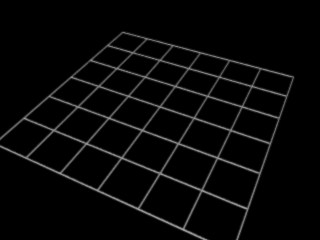
\includegraphics[width=6cm]{pics/grid}
\end{center}
\end{funcdesc}

\section{\module{noise} ---
         Noise functions}

\declaremodule{extension}{cgkit.noise}
\modulesynopsis{A set of basic noise functions}

\begin{funcdesc}{noise}{x[, y[, z[,t]]]}
Returns a noise value (Perlin) in the range from 0 to 1. The arguments
can be up to 4 floating point values or a sequence with up to 4
floating point values (e.g. a \class{vec3} or a \class{vec4}) with an
optional time value. The return value is a pseudo random number in the
range from 0 to 1. Due to the nature of this noise implementation
(gradient noise) the return value at integer lattice points is always 0.5.

As an example, here is a 2D slice (the grid shows the integer lattice):

\begin{center}
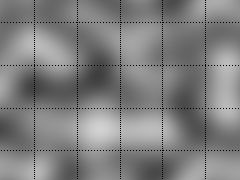
\includegraphics[width=6cm]{pics/noise}
\end{center}

\note{The actual function call depends on the number of arguments, so
calling noise(x,y) is not the same as calling noise(x,y,0). The former
case is a true 2D noise whereas the latter is 3D. The same difference
exists between 3D and 4D.}
\end{funcdesc}

\begin{funcdesc}{snoise}{x[, y[, z[,t]]]}
Returns a signed noise value (Perlin) in the range from -1 to 1. A
call to \code{snoise(args)} is equivalent to \code{2*noise(args)-1}.
\end{funcdesc}

\begin{funcdesc}{pnoise}{point[, t], period[, tperiod]}
Periodic noise function. Basically this is the same as
\function{noise()} but with a periodic return value: \function{pnoise(point)} =
\function{pnoise(point+period)}. The time value can be either part of the point
or it can be specified separately. The point and period must always
have the same dimension. The return value is in the range from 0 to 1.
\end{funcdesc}

\begin{funcdesc}{spnoise}{point[, t], period[, tperiod]}
Signed periodic noise function. The return value is in the range from
-1 to 1. A call to \code{spnoise(args)} is equivalent to 
\code{2*pnoise(args)-1}.
\end{funcdesc}

\begin{funcdesc}{cellnoise}{x[, y[, z[,t]]]}
Returns a pseudo random number which is constant between integer
lattice points. The return value is in the range from 0 to 1.

As an example, here is a 2D slice (the grid shows the integer lattice):

\begin{center}
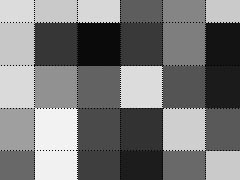
\includegraphics[width=6cm]{pics/cellnoise}
\end{center}
\end{funcdesc}

\begin{funcdesc}{scellnoise}{x[, y[, z[,t]]]}
Signed cell noise. The return value is in the range from -1 to 1. A
call to \code{scellnoise(args)} is equivalent to \code{2*cellnoise(args)-1}.
\end{funcdesc}

\begin{funcdesc}{fBm}{point, octaves, lacunarity=2.0, gain=0.5}
Fractional Brownian motion. The argument point must be a sequence of
either 2 or 3 float values (e.g. a \class{vec3}). This function is a sum of
noise values with different frequencies and amplitudes and is
equivalent to the following code:

\begin{verbatim}
sum = 0.0
amp = 1.0
for i in range(octaves):
    sum += amp*snoise(point)
    amp *= gain
    point *= lacunarity
\end{verbatim}

The return value is in the range from 0 to 1.

As an example, here is a 2D slice (the grid shows the integer lattice):

\begin{center}
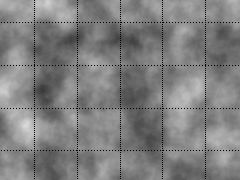
\includegraphics[width=6cm]{pics/fbm}
\end{center}
\end{funcdesc}

\begin{funcdesc}{turbulence}{point, octaves, lacunarity=2.0, gain=0.5}
The code of the turbulence function is very similar to \function{fBm()}. The
difference is that it sums up \code{abs(snoise())} instead of \code{noise()}. 
However, the return value is in the range from 0 to 1.

As an example, here is a 2D slice (the grid shows the integer lattice):

\begin{center}
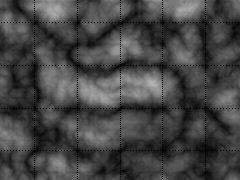
\includegraphics[width=6cm]{pics/turbulence}
\end{center}
\end{funcdesc}


All of the above functions have a vector version that take the same
input parameters but return a vector as result. The output always has
the same dimension than the input. If the time value is specified
separately it does not count to the dimension. For example a call to
\code{vnoise((x,y,z))} returns a \class{vec3}, just as a call to
\code{vnoise((x,y,z),t)}. However, a call to \code{vnoise((x,y,z,t))} 
returns a \class{vec4}.

\begin{funcdesc}{vnoise}{x[, y[, z[,t]]]}
See \function{noise()}.
\end{funcdesc}

\begin{funcdesc}{vsnoise}{x[, y[, z[,t]]]}
See \function{snoise()}.
\end{funcdesc}

\begin{funcdesc}{vpnoise}{point[, t], period[, tperiod]}
See \function{pnoise()}.
\end{funcdesc}

\begin{funcdesc}{vspnoise}{point[, t], period[, tperiod]}
See \function{spnoise()}.
\end{funcdesc}

\begin{funcdesc}{vcellnoise}{x[, y[, z[,t]]]}
See \function{cellnoise()}.
\end{funcdesc}

\begin{funcdesc}{vscellnoise}{x[, y[, z[,t]]]}
See \function{scellnoise()}.
\end{funcdesc}

\begin{funcdesc}{vfBm}{point, octaves, lacunarity=2.0, gain=0.5}
See \function{fBm()}.
\end{funcdesc}

\begin{funcdesc}{vturbulence}{point, octaves, lacunarity=2.0, gain=0.5}
See \function{turbulence()}.
\end{funcdesc}

\section{\module{sl} ---
         RenderMan Shading Language functionality}

\declaremodule{extension}{cgkit.sl}
\modulesynopsis{Provides the same functions than the RenderMan Shading Language}

This module provides some of the functionality from the RenderMan
Shading Language. Those functions that require an actual rendering
context (surfaces, light sources, etc.) are not supported.

Most of the functions can be used just like in the Shading
Language. An exception are those functions whose return type is
dependant on the context as it is the case with \function{random()} or
\function{noise()}. Here, those functions have to be prepended with the 
return type, for example \function{float_random()} or 
\function{point_noise()} (that is, the cast is part of the name).

%----
\subsection{Constants}

\begin{datadesc}{PI}
This is the same as \code{math.pi}.
\end{datadesc}

%-----
\subsection{Math functions}

\begin{funcdesc}{abs}{x}
Returns the absolute value of its argument. This is just the builtin
\function{abs()} function.
\end{funcdesc}

\begin{funcdesc}{acos}{a}
Returns the arc cosine. This function is imported from the
\module{math} module.
\end{funcdesc}

\begin{funcdesc}{asin}{a}
Returns the arc sine. This function is imported from the \module{math} module.
\end{funcdesc}

\begin{funcdesc}{atan}{y[, x]}
Returns the arc tangent. With one argument \function{math.atan()} is
called, with two arguments \function{math.atan2()} is called.
\end{funcdesc}

\begin{funcdesc}{ceil}{x}
Returns the largest integer not greater than \var{x}. This function is
imported from the \module{math} module.
\end{funcdesc}

\begin{funcdesc}{clamp}{x, min, max}
Returns \var{min} if \var{x} < \var{min}, \var{max} if \var{x} > \var{max}, 
otherwise \var{x}.
\end{funcdesc}

\begin{funcdesc}{color_cellnoise}{p}
Returns a color value (actually a \class{vec3}) whose value is a (pseudo)
random function of its arguments. The return value is constant between
integer lattice points.
\end{funcdesc}

\begin{funcdesc}{color_noise}{p}
Returns a color value (actually a \class{vec3}) whose value is a (pseudo)
random function of its arguments.
\end{funcdesc}

\begin{funcdesc}{color_pnoise}{p, period}
Returns a color value (actually a \class{vec3}) whose value is a periodic
(pseudo) random function of its arguments.
\end{funcdesc}

\begin{funcdesc}{color_random}{}
Return a color whose componenets are a random number between 0 and
1. The function actually returns a \class{vec3}.
\end{funcdesc}

\begin{funcdesc}{cos}{a}
Returns the cosine. This function is imported from the \module{math} module.
\end{funcdesc}

\begin{funcdesc}{degrees}{rad}
Converts from radians to degrees.
\end{funcdesc}

\begin{funcdesc}{exp}{x}
Returns \code{pow(e,x)}. This function is imported from the
\module{math} module.
\end{funcdesc}

\begin{funcdesc}{float_cellnoise}{p}
Returns a float value which is a (pseudo) random function of its
arguments. The return value is constant between integer lattice
points. This function is imported from the \module{noise} module.
\end{funcdesc}

\begin{funcdesc}{float_noise}{p}
Returns a float value which is a (pseudo) random function of its
arguments. This function is imported from the \module{noise} module.
\end{funcdesc}

\begin{funcdesc}{float_pnoise}{p, period}
Returns a float value which is a periodic (pseudo) random function of
its arguments. This function is imported from the \module{noise} module.
\end{funcdesc}

\begin{funcdesc}{float_random}{}
Return a random number between 0 and 1. This call is equivalent to
\function{random.random()}.
\end{funcdesc}

\begin{funcdesc}{floor}{x}
Returns the smallest integer not smaller than \var{x}. This function is
imported from the \module{math} module.
\end{funcdesc}

\begin{funcdesc}{inversesqrt}{x}
Returns \code{1/sqrt(x)}.
\end{funcdesc}

\begin{funcdesc}{log}{x[, base]}
Returns the natural logarithm of \var{x} (the same as
\function{math.log}) or the logarithm to the specified base.
\end{funcdesc}

\begin{funcdesc}{max}{a, b, ...}
Returns the argument with maximum value. This is just the builtin
\function{max()} function.
\end{funcdesc}

\begin{funcdesc}{min}{a, b, ...}
Returns the argument with minimum value. This is just the builtin 
\function{min()} function.
\end{funcdesc}

\begin{funcdesc}{mix}{val0, val1, t}
For \var{t}=0 the value \var{val0} is returned, for \var{t}=1 the value 
\var{val1} is returned. For values of \var{t} between 0 and 1 a linearly 
interpolated value is returned.
\end{funcdesc}

\begin{funcdesc}{mod}{a, b}
Returns \code{a\%b}. This is just an equivalent for the \%-operator.
\end{funcdesc}

\begin{funcdesc}{point_cellnoise}{p}
Returns a point (as a \class{vec3}) whose value is a (pseudo) random
function of its arguments. The return value is constant between
integer lattice points.
\end{funcdesc}

\begin{funcdesc}{point_noise}{p}
Returns a point (as a \class{vec3}) whose value is a (pseudo) random function
of its arguments.
\end{funcdesc}

\begin{funcdesc}{point_pnoise}{p, period}
Returns a point (as a \class{vec3}) whose value is a periodic (pseudo) random
function of its arguments.
\end{funcdesc}

\begin{funcdesc}{point_random}{}
Return a point (a \class{vec3}) whose componenets are a random number between
0 and 1.
\end{funcdesc}

\begin{funcdesc}{pow}{x, y}
Returns x**y. This function is imported from the \module{math} module.
\end{funcdesc}

\begin{funcdesc}{radians}{deg}
Converts from degrees to radians.
\end{funcdesc}

\begin{funcdesc}{round}{deg}
Returns the integer closest to \var{x}. This is just the builtin 
\function{round()} function.
\end{funcdesc}

\begin{funcdesc}{sign}{x}
Returns -1 with a negative argument, +1 with a positive argument, and
0 if its argument is zero.
\end{funcdesc}

\begin{funcdesc}{sin}{a}
Returns the sine. This function is imported from the \module{math} module.
\end{funcdesc}

\begin{funcdesc}{smoothstep}{min, max, value}
Returns 0 if \var{value} < \var{min}, 1 if \var{value} > \var{max},
and performs a smooth Hermite interpolation between 0 and 1 in the
interval \var{min} to \var{max}.
\end{funcdesc}

\begin{funcdesc}{spline}{t, controlpoints}
Fits a spline to the control points given and returns the value at \var{t}
which ranges from 0 to 1. At least four control points must always be
given.
\end{funcdesc}

\begin{funcdesc}{sqrt}{x}
Returns the square root. This function is imported from the \module{math}
module.
\end{funcdesc}

\begin{funcdesc}{step}{min, x}
Returns 0 if \var{x} < \var{min}, otherwise 1.
\end{funcdesc}

\begin{funcdesc}{tan}{a}
Returns the tangent. This function is imported from the \module{math} module.
\end{funcdesc}

\begin{funcdesc}{tan}{a}
Returns the tangent. This function is imported from the \module{math} module.
\end{funcdesc}

\begin{funcdesc}{vector_cellnoise}{p}
Returns a vector (as a \class{vec3}) whose value is a (pseudo) random function
of its arguments. The return value is constant between integer lattice
points.
\end{funcdesc}

\begin{funcdesc}{vector_noise}{p}
Returns a vector (as a \class{vec3}) whose value is a (pseudo) random function
of its arguments.
\end{funcdesc}

\begin{funcdesc}{vector_pnoise}{p, period}
Returns a vector (as a \class{vec3}) whose value is a periodic (pseudo) random
function of its arguments.
\end{funcdesc}

%-----
\subsection{Geometric functions}

\begin{funcdesc}{distance}{p1, p2}
Returns the distance between two points. The arguments should be of type 
\class{vec3}.
\end{funcdesc}

\begin{funcdesc}{faceforward}{N, I, Nref}
Flips \var{N} so that it faces in the direction opposite to \var{I}. 

\note{In contrast to the Shading Language \var{Nref} is not optional.}
\end{funcdesc}

\begin{funcdesc}{length}{v}
Returns the length of a vector. This is equivalent to calling 
\method{v.length()}.
\end{funcdesc}

\begin{funcdesc}{normalize}{v}
Returns a unit vector in the direction of \var{v}. This is equivalent to
calling \method{v.normalize()}.
\end{funcdesc}

\begin{funcdesc}{ptlined}{p0, p1, q}
Returns the distance between point \var{q} and the line segment \var{p0},
\var{p1}. The arguments should be of type \class{vec3}.
\end{funcdesc}

\begin{funcdesc}{reflect}{I, N}
Returns the reflection vector given an incident direction \var{I} and a
normal vector \var{N}. This is equivalent to calling \method{I.reflect(N)}.
\end{funcdesc}

\begin{funcdesc}{refract}{I, N, eta}
Returns the transmitted vector given an incident direction \var{I},
the normal vector \var{N} and the relative index of refraction
\var{eta}. This is equivalent to calling \method{I.refract(N, eta)}.
\end{funcdesc}

\begin{funcdesc}{xcomp}{p}
Return the x component of \var{p}. This is equivalent to \code{p.x}.
\end{funcdesc}

\begin{funcdesc}{ycomp}{p}
Return the y component of \var{p}. This is equivalent to \code{p.y}.
\end{funcdesc}

\begin{funcdesc}{zcomp}{p}
Return the z component of \var{p}. This is equivalent to \code{p.z}.
\end{funcdesc}

\begin{funcdesc}{setxcomp}{p, x}
Set the x component of \var{p}. This is equivalent to \code{p.x = x}.
\end{funcdesc}

\begin{funcdesc}{setycomp}{p, y}
Set the y component of \var{p}. This is equivalent to \code{p.y = y}.
\end{funcdesc}

\begin{funcdesc}{setzcomp}{p, z}
Set the z component of \var{p}. This is equivalent to \code{p.z = z}.
\end{funcdesc}

\begin{funcdesc}{comp}{c, index}
Get an individual color component. This is equivalent to \code{c[index]}.
\end{funcdesc}

\begin{funcdesc}{setcomp}{c, index, value}
Set an individual color component. This is equivalent to 
\code{c[index] = value}.
\end{funcdesc}

%-----
\subsection{String functions}

\begin{funcdesc}{concat}{str1, ..., strn}
Returns a concatenated string.
\end{funcdesc}

\begin{funcdesc}{format}{pattern, val1, val2, ..., valn}
Returns a formatted string (similar to the C function
\cfunction{sprintf()}). Any occurance of the character \% followed by a
letter is replaced by a value. In this implementation it doesn't
matter what letter you are actually using (in the Shading Language it
would be \%f for floats, \%p for points, vectors or normals, \%c for
colors, \%m for matrices and \%s for strings).
\end{funcdesc}

\begin{funcdesc}{match}{pattern, subject}
String pattern matching.
\end{funcdesc}

\begin{funcdesc}{printf}{pattern, val1, val2, ..., valn}
Prints the values of the specified variables. Any occurance of the
character \% followed by a letter is replaced by a value. In this
implementation it doesn't matter what letter you are actually using (in
the Shading Language it would be \%f for floats, \%p for points, vectors
or normals, \%c for colors, \%m for matrices and \%s for strings).
\end{funcdesc}

%-----
\subsection{Unsupported functions}

The following functions are not supported by this module:

\begin{itemize}
\item \cfunction{Du()}
\item \cfunction{Dv()}
\item \cfunction{Deriv()}
\item \cfunction{filterstep()}
\end{itemize}

\begin{itemize}
\item \cfunction{area()}
\item \cfunction{calculatenormal()}
\item \cfunction{depth()}
\item \cfunction{fresnel()}
\item \cfunction{transform()}
\item \cfunction{vtransform()}
\item \cfunction{ntransform()}
\end{itemize}

\begin{itemize}
\item \cfunction{ambient()}
\item \cfunction{diffuse()}
\item \cfunction{phong()}
\item \cfunction{specular()}
\item \cfunction{specularbrdf()}
\item \cfunction{trace()}
\end{itemize}

\begin{itemize}
\item \cfunction{environment()}
\item \cfunction{shadow()}
\item \cfunction{texture()}
\item \cfunction{textureinfo()}
\end{itemize}

\begin{itemize}
\item \cfunction{atmosphere()}
\item \cfunction{displacement()}
\item \cfunction{incident()}
\item \cfunction{lightsource()}
\item \cfunction{opposite()}
\item \cfunction{surface()}
\end{itemize}

\begin{itemize}
\item \cfunction{attribute()}
\item \cfunction{option()}
\item \cfunction{rendererinfo()}
\end{itemize}

\section{\module{sltokenize} ---
          Tokenizer for the RenderMan Shading Language}

\declaremodule{extension}{cgkit.sltokenize}
\modulesynopsis{Tokenizer for the RenderMan Shading Language}

This module provides a lexical scanner for the RenderMan Shading
Language. You use it in the same way as the Python tokenize module is
used.

\begin{funcdesc}{tokenize}{readline, tokeneater}
Reads an input stream and creates tokens. The first parameter,
\var{readline}, must be a callable object which provides the same interface
as the \method{readline()} method of built-in file objects. Each call to the
function should return one line of input as a string.

The second parameter, \var{tokeneater}, must also be a callable
object. It is called with six parameters: the token type, the token
string, a tuple (srow, scol) specifying the row and column where the
token begins in the source, a tuple (erow, ecol) giving the ending
position of the token, the line on which the token was found and the
filename of the current file.

The token type can be one of 

\begin{itemize}
\item \code{WHITESPACE}: This is a series of blanks and/or tabs. 
\item \code{NAME}: A valid identifier name or keyword. 
\item \code{NUMBER}: An integer or float. 
\item \code{STRING}: A string enclosed in '"'. 
\item \code{NEWLINE}: A newline character. 
\item \code{OPERATOR}: An operator such as '+', '-', '!', '==', '!=', etc. 
\item \code{CHARACTER}: A single character that doesn't fit anything else. 
\item \code{TYPE}: A Shading Language type (float, point, vector, normal, matrix, color) 
\end{itemize}

By default, the filename argument is an empty string. It will only be
the actual filename if you provide a preprocessed file stream as input
(so you should first run \code{cpp} on any shader). The tokenizer
actually expects preprocessed data as it does not handle comments.
\end{funcdesc}

\section{\module{slparams} ---
          Extracting RenderMan Shader parameters}
\label{slparams}

\declaremodule{extension}{cgkit.slparams}
\modulesynopsis{Extracting RenderMan Shader parameters}

This module can be used to extract the parameters of a RenderMan
shader either from the shader source file or from the compiled shader.
To read parameters from a compiled shader it is necessary that the renderer
package is installed that was used to compile the shader. Currently, the
following renderers are supported:

\begin{itemize}
  \item 3Delight 
  \item Aqsis
  \item Pixie
  \item PRMan
\end{itemize}

Other renderers can be added at runtime (see the \module{sloargs} module).

\begin{funcdesc}{slparams}{slfile, cpp=None, cpperrstream=sys.stderr, includedirs=None, defines=None}
Extracts the shader parameters from a Shading Language source file. 

The argument \var{slfile} is either the name of a compiled shader, the
name of the shader source file (*.sl) or a file-like object that provides the
shader sources.

\var{cpp} determines how the shader source is preprocessed. It can be
either a string containing the name of an external preprocessor tool
(such as \code{cpp}) that must take the file name as parameter and
dump the preprocessed output to stdout. If the preprocessor does not
produce any data a \exception{PreprocessorNotFound} exception is
thrown. The error stream of the preprocessor is written to the object
that is specified by \var{cpperrstream} which must have a
\method{write()} method. If \var{cpperrstream} is \code{None}, the error 
stream is ignored. \var{cpp} can also be a callable object that takes a
filename as input and returns the filtered contents as a string. If
\var{cpp} is \code{None} a simple internal preprocessor based on the 
\module{simplecpp} module is used.

\var{includedirs} is a list of strings that contain directories where to 
look for include files. \var{defines} is a list of tuples (\var{name},
\var{value}) that specify the predefined symbols to use.

The function returns a list of shader info objects. These objects have
four attributes:
    
\begin{itemize}
  \item \var{type}: The type of the shader (\code{"surface"},
  \code{"displacement"}, etc.)
  \item \var{name}: The name of the shader
  \item \var{params}: The shader parameters (see below)
  \item \var{meta}: The shader meta data. How exactly meta data is specified
  depends on the renderer you are using.
\end{itemize}
     
The parameters are given as a list of shader parameter objects describing each
parameter. A shader parameter object has the following attributes:

\begin{itemize}
\item \var{outputSpec}: The output specifier (either \code{"output"} or an empty
string)
\item \var{storage}: The storage class (\code{"uniform"} or \code{"varying"}) 
\item \var{type}: The parameter type 
\item \var{size}: The array length or \code{None} if the parameter is not
an array
\item \var{name}: The name of the parameter 
\item \var{space}: The space in which a point-like type or a color was
defined. If the parameter is an array then this is also an array of space names.
\item \var{default}: The "raw" default value. If the input was a shader source file,
  this will always be a string containing an expression. If the input was
  a compiled shader this will already be an appropriate Python value.
  You should never use this value directly, but always use
  \function{convertdefault()} to obtain a value which can be further processed.
  This way, your code will work for both, compiled shaders and shader source files.
\end{itemize}

For backwards compatibility, the shader info object behaves like a
3-tuple (\var{type}, \var{name}, \var{params}). The meta data can only be
accessed via name though. The shader parameter objects can also be used
like 7-tuples containing the above data (in the order given above).

Example (output slightly reformatted for better readability):
 
\begin{verbatim}
>>> from cgkit import slparams
>>> shaders = lparams.slparams("plastic.sl")
>>> print shaders
[('surface', 'plastic', 
  [('', 'uniform', 'float', None, 'Ka', None, '1'),
   ('', 'uniform', 'float', None, 'Kd', None, '0.5'),
   ('', 'uniform', 'float', None, 'Ks', None, '0.5'),
   ('', 'uniform', 'float', None, 'roughness', None, '0.1'),
   ('', 'uniform', 'color', None, 'specularcolor', 'rgb', '1')])]
>>> shaders[0].type
'surface'
>>> shaders[0].name
'plastic'
>>> for param in shaders[0].params: print param.name
... 
Ka
Kd
Ks
roughness
specularcolor
>>> shaders[0].meta
{}
\end{verbatim}

The parser used inside this function was generated using the parser
generator \ulink{Yapps}{http://theory.stanford.edu/\~{}amitp/Yapps/} 
by Amit Patel.
\end{funcdesc}

\begin{funcdesc}{convertdefault}{paramtuple}
Converts the default value of a shader parameter into a Python
type. The argument \var{paramtuple} must be a 7-tuple (or parameter object) as
returned by \function{slparams()}. The function returns a Python object that corresponds to
the default value of the parameter. If the default value can't be
converted then \code{None} is returned. Only the functions that are
present in the \module{sl} module are evaluated. If a default value
calls a user defined function then \code{None} is returned. The SL
types will be converted into the following Python types:

\begin{tableii}{c|c}{code}{SL type }{ Python type}
\lineii{float}{\code{float}}
\lineii{string}{\code{string}}
\lineii{color}{\code{vec3}}
\lineii{point}{\code{vec3}}
\lineii{vector}{\code{vec3}}
\lineii{normal}{\code{vec3}}
\lineii{matrix}{\code{mat4}}
\end{tableii}

Arrays will be converted into lists of the corresponding type.
\end{funcdesc}

The module defines the following exception classes:

\begin{excdesc}{SLParamsError}
Base class for the exceptions in this module. This class is derived
from the Exception class.
\end{excdesc}

\begin{excdesc}{PreprocessorNotFound}
This exception is thrown when calling the preprocessor didn't produce
any data.
\end{excdesc}

\begin{excdesc}{SyntaxError}
This exception is thrown when a syntax error is found in any function
or shader definition. The exception has the following attributes:

\begin{itemize}
\item \var{filename}: The filename where the error was found 
\item \var{lineno}: The line number where the error was found 
\item \var{line}: The entire line that contains the error 
\item \var{errpos}: The character position where the error token starts
\end{itemize}
\end{excdesc}

\begin{excdesc}{NoMoreTokens}
This exception is thrown when the parser runs out of tokens.
\end{excdesc}

\section{\module{glslangtokenize} ---
          Tokenizer for the OpenGL 2 shading language}

\declaremodule{extension}{cgkit.glslangtokenize}
\modulesynopsis{Tokenizer for the OpenGL 2 shading language}

This module provides a lexical scanner for the OpenGL 2 shading language.
You use it in the same way as the Python tokenize module is used.

\begin{funcdesc}{tokenize}{readline, tokeneater}
Reads an input stream and creates tokens. The first parameter,
\var{readline}, must be a callable object which provides the same interface
as the \method{readline()} method of built-in file objects. Each call to the
function should return one line of input as a string.

The second parameter, \var{tokeneater}, must also be a callable
object. It is called with six parameters: the token type, the token
string, a tuple (srow, scol) specifying the row and column where the
token begins in the source, a tuple (erow, ecol) giving the ending
position of the token, the line on which the token was found and the
filename of the current file.

The token type can be one of 

\begin{itemize}
\item \code{WHITESPACE}: This is a series of blanks and/or tabs. 
\item \code{NAME}: A valid identifier name or keyword. 
\item \code{NUMBER}: An integer or float. 
\item \code{STRING}: A string enclosed in '"'. 
\item \code{NEWLINE}: A newline character. 
\item \code{OPERATOR}: An operator such as '+', '-', '!', '==', '!=', etc. 
\item \code{CHARACTER}: A single character that doesn't fit anything else. 
\item \code{TYPE}: A language type (void, bool, float, int, vec2, vec3, vec4, etc.)
\item \code{QUALIFIER}: A type qualifier (const, attribute, uniform, varying, in, out, inout)
\end{itemize}

By default, the filename argument is an empty string. It will only be
the actual filename if you provide a preprocessed file stream as input
(so you should first run \code{cpp} on any shader). The tokenizer
actually expects preprocessed data as it does not handle comments.
\end{funcdesc}

\section{\module{glslangparams} ---
          Extracting OpenGL 2 shader parameters}
\label{slparams}

\declaremodule{extension}{cgkit.glslangparams}
\modulesynopsis{Extracting OpenGL 2 shader parameters}

This module can be used to extract the parameters of an OpenGL 2 shader
from the shader source file.

\begin{funcdesc}{glslangparams}{shader, cpp=None, cpperrstream=sys.stderr}
Extracts the shader parameters from an OpenGL 2 shader source file.

The argument \var{shader} is either the name of the shader source file or a
file-like object that provides the shader sources. \var{cpp} determines how
the shader source is preprocessed. It can either be a string
containing the name of an external preprocessor tool (such as \code{'cpp'})
that must take the file name as parameter and dump the preprocessed
output to stdout or it can be a callable that takes \var{shader} and
\var{cpperrstream} as input and returns the preprocessed sources as a
string. If the external preprocessor does not produce any data a
\exception{PreprocessorNotFound} exception is thrown.  The error stream of the
preprocessor is written to the object that is specified by
\var{cpperrstream} which must have a write() method. If \var{cpperrstream} is
\code{None}, the error stream is ignored.

If \var{cpp} is None a simple internal preprocessor based on the 
\module{simplecpp} module is used.

The function returns three lists (\var{uniform}, \var{attribute}, 
\var{varying}) that contain the variables with the corresponding qualifier.

A uniform variable is a 5-tuple (\var{type}, \var{identifier}, \var{arraysize},
\var{structname}, \var{struct}). \var{arraysize} is a string containing 
the expression for the length of the array (i.e. the value between the
square brackets). If the variable is no array, \var{arraysize} is
\code{None}.  When the variable is a struct, \var{type} has the value
\code{'struct'}. In this case, the struct is given in \var{struct} (which is
itself a list of variables as 5-tuples). If the struct has a name,
this name is given in \var{structname}, otherwise \var{structname} is 
\code{None}.

An attribute variable is a 2-tuple (\var{type}, \var{identifier}) and a 
varying variable is a 3-tuple (\var{type}, \var{identifier}, \var{arraysize}) 
where \var{arraysize} is defined as in the uniform case.
\end{funcdesc}

The module defines the following exception class:

\begin{excdesc}{GLSLangParseError}
This exception is thrown when an error occurs during parsing the shader
source file.
\end{excdesc}

\section{\module{spacedevice} ---
          Wrapper around the 3Dconnexion Developer's Kits}

\declaremodule{extension}{cgkit.spacedevice}
\modulesynopsis{Wrapper around the 3Dconnexion Developer's Kits}

The \module{spacedevice} module allows applications to support
3D input devices such as a SpaceMouse or a SpaceBall. The module
wraps the 3DxWare SDK by 3Dconnexion. For a more detailed description
of the SDK see the documentation that is part of the
\ulink{SDK}{http://www.3dconnexion.com/sdk.htm}.

The module has to be used in conjunction with a GUI toolkit as there must
be a window that receives the 3D input device events. In principle, any
GUI toolkit can be used as long as it allows obtaining the native windows
handle and accessing system events. The steps necessary to use a 3D input
device are as follows:

\begin{enumerate}
\item Create a \class{SpaceDevice} object.
\item Open the device using the \method{open()} method. This requires a windows
handle of the window that will receive the SpaceDevice events.
\item For every system event received call the \method{translateWin32Event()}
method and check if the event was generated by a SpaceDevice.
If it was, check for the event type and process the event.
\item When the application terminates, call the \method{close()} method to
close the device.

\end{enumerate}

% available()
\begin{funcdesc}{available}{}
Returns \code{True} if the module functionality is available. Currently,
this function will only return \code{True} under Windows and if the
functionality was enabled during compilation.

If this function returns \code{False}, an exception will be raised
whenever you try to instantiate a class from this module.
\end{funcdesc}


\begin{classdesc}{SpaceDevice}{}
The \class{SpaceDevice} class provides the interface to the 3DxWare
library that is used to communicate with the 3D input device. The
constructor of this class calls the SDK function \cfunction{SiInitialize()} 
to initialize the 3DxWare library. The destructor closes the device if
it is open and calls \cfunction{SiTerminate()}.
\end{classdesc}

% open
\begin{methoddesc}{open}{appname, hwnd, devID=SI_ANY_DEVICE}
Establish a connection to a 3D input device. \var{appname} is a string
containing the application name, \var{hwnd} is the native window handle 
(as integer) of the window that should receive the events. \var{devID}
is the device id. An exception is thrown if a connection cannot be
established.

This method calls the SDK functions \cfunction{SiOpenWinInit()} and
\cfunction{SiOpen()}.
\end{methoddesc}

% close
\begin{methoddesc}{close}{}
Close the connection to a device. The function returns immediately if
there is no open connection.

This method calls the SDK function \cfunction{SiClose()}.
\end{methoddesc}

% translateWin32Event
\begin{methoddesc}{translateWin32Event}{msgid, wparam, lparam}
Translates a Win32 event into a SpaceDevice event. The return value is
a tuple (\var{RetVal}, \var{EventType}, \var{Data}).

\var{RetVal} is an object of type
\code{RetVal} that represents an enumeration. It is 
\code{RetVal.IS_EVENT} if the event was generated by a 3D input device,
otherwise it is \code{RetVal.NOT_EVENT}.

\var{EventType} is an object of type \code{EventType} that again represents
an enumeration. It can take one of the following values:

\begin{itemize}
\item \code{EventType.BUTTON_EVENT}
\item \code{EventType.MOTION_EVENT}
\item \code{EventType.ZERO_EVENT}
\item \code{EventType.EXCEPTION_EVENT}
\end{itemize}

The contents of the third value, \var{Data}, depend on the event type:

\begin{tableii}{l|l}{code}{Event type}{Data}
\lineii{BUTTON_EVENT}{(\var{pressed}, \var{released})}
\lineii{MOTION_EVENT}{(\var{translation}, \var{rotation}, \var{period})}
\lineii{ZERO_EVENT}{\code{None}}
\lineii{EXCEPTION_EVENT}{\code{None}}
\end{tableii}

\var{pressed} and \var{released} are each lists that contain the numbers
of the button that were either pressed or released. \var{translation}
is a 3-tuple containing the translation vector and \var{rotation} is a
3-tuple containing the rotation vector. \var{period} contains the time
in milliseconds since the last device event.

This method calls the SDK functions \cfunction{SiGetEventWinInit()} and
\cfunction{SiGetEvent()}.
\end{methoddesc}

% beep
\begin{methoddesc}{beep}{s}
Causes the device to emit a sequence of tones and pauses that is
encoded in the string \var{s}. Lowercase letters represent a tone,
uppercase letters represent a pause.  The closer the letter is to the
beginning of the alphabet the shorter the pause or tone.

This method calls the SDK function \cfunction{SiBeep()}.
\end{methoddesc}

% getDeviceID
\begin{methoddesc}{getDeviceID}{}
Return the device id of the currently open device. 

This method calls the SDK function \cfunction{SiGetDeviceID()}.
\end{methoddesc}

% getDeviceInfo
\begin{methoddesc}{getDeviceInfo}{}
Return information about the currently open device. The return value
is a 5-tuple (\var{device type}, \var{numButtons}, \var{numDegrees},
\var{canBeep}, \var{firmware}). 

This method calls the SDK function \cfunction{SiGetDeviceInfo()}.
\end{methoddesc}

% getDriverInfo
\begin{methoddesc}{getDriverInfo}{}
Return version information about the driver. The return value is a 5-tuple
(\var{major}, \var{minor}, \var{build}, \var{versionstr}, \var{datestr}).

This method calls the SDK function \cfunction{SiGetDriverInfo()}.
\end{methoddesc}

% getNumDevices
\begin{methoddesc}{getNumDevices}{}
Return the number of input devices detected by the driver. 

This method calls the SDK function \cfunction{SiGetNumDevices()}.
\end{methoddesc}

% rezero
\begin{methoddesc}{rezero}{}
Causes the input device's current setting to be defined as the rest
position. 

This method calls the SDK function \cfunction{SiRezero()}.
\end{methoddesc}

% setUIMode
\begin{methoddesc}{setUIMode}{show}
Change the state of the driver menu window from within an application. The
function has to be called before a call to \method{open()}.
\var{show} is a boolean that specifies if the driver menu should be displayed
or not.

This method calls the function \cfunction{SiSetUiMode()}.
\end{methoddesc}


\begin{notice}[note]
The module uses the SDK by 3Dconnexion which can be found at 
\url{http://www.3dconnexion.com/sdk.htm}. The following is the
copyright information of the SDK:

{\em (C) 1998-2001 3Dconnexion 

Permission to use, copy, modify, and distribute this software for all
purposes and without fees is hereby granted provided that this
copyright notice appears in all copies. Permission to modify this
software is granted and 3Dconnexion will support such modifications
only if said modifications are approved by 3Dconnexion}
\end{notice}

% -------------------------------------------------------
\subsection{Example}

Here is a code example that uses pygame (you need at least version 1.7.1)
as GUI toolkit. It simply prints the input device events to the console.

\begin{verbatim}
######################################################################
# SpaceDevice demo
#
# This demo demonstrates the usage of the SpaceDevice object in the
# cgkit.spacedevice module which can be used to access events from
# a SpaceMouse or SpaceBall. You can use this module to add support
# for a SpaceDevice in your own Python application. The demo simply
# prints the events generated from a SpaceDevice to the console.
#
# This demo uses pygame as GUI toolkit (v1.7.1 is required).
# You can use any other GUI toolkit as long as it 1) lets you obtain
# the native window handle of a window and 2) provides access to
# system events.
######################################################################
\end{verbatim}

\begin{verbatim}
import sys
import pygame
from pygame.locals import *
from cgkit import spacedevice
\end{verbatim}

\begin{verbatim}
# handleSystemEvent
def handleSystemEvent(evt):
    """Handle a system event.

    evt is a pygame event object that contains a system event. The function
    first checks if the event was generated by a SpaceDevice and if it was,
    it prints the event data.
    """
    # sdev is the global SpaceDevice object
    global sdev
    
    # Translate the system event into a SpaceDevice event...
    res, evttype, data = sdev.translateWin32Event(evt.msg, evt.wparam, evt.lparam)
    # Check if the event actually was an event generated from
    # the SpaceMouse or SpaceBall...
    print res
    if res!=spacedevice.RetVal.IS_EVENT:
        return

    # Motion event?
    if evttype==spacedevice.EventType.MOTION_EVENT:
        t,r,period = data
        print "Motion: trans:%s rot:%s period:%d"%(t, r, period)
    # Button event?
    elif evttype==spacedevice.EventType.BUTTON_EVENT:
        pressed, released = data
        print "Button: pressed:%s released:%s"%(pressed, released)
    # Zero event?
    elif evttype==spacedevice.EventType.ZERO_EVENT:
        print "Zero"
\end{verbatim}    

\begin{verbatim}
######################################################################

# Check if cgkit was compiled with SpaceDevice support...
if not spacedevice.available():
    print "No SpaceDevice functionality available"
    sys.exit(1)
    
# Initialize pygame...
passed, failed = pygame.init()
if failed>0:
    print "Error initializing pygame"
    sys.exit(1)
\end{verbatim}

\begin{verbatim}
# Open a window...
pygame.display.set_caption("SpaceDevice demo")
srf = pygame.display.set_mode((640,480))

# Enable system events...
pygame.event.set_allowed(SYSWMEVENT)

# Initialize the Space Device...
sdev = spacedevice.SpaceDevice()
info = pygame.display.get_wm_info()
hwnd = info["window"]
sdev.open("Demo", hwnd)
\end{verbatim}

\begin{verbatim}
# Print some information about the driver and the device...
major, minor, build, versionstr, datestr = sdev.getDriverInfo()
print "Driver info:"
print "------------"
print "%s, v%d.%d.%d, %s\n"%(versionstr, major, minor, build, datestr)

devtyp, numbuttons, numdegrees, canbeep, firmware = sdev.getDeviceInfo()
print "Device info:"
print "------------"
print "Device ID:",sdev.getDeviceID()
print "Type     :",devtyp
print "#Buttons :",numbuttons
print "#Degrees :",numdegrees
print "Can beep :",canbeep
print "Firmware :",firmware
print ""
\end{verbatim}

\begin{verbatim}
# Event loop...
running = True
while running:

    # Get a list of events...
    events = pygame.event.get()

    # Process the events...
    for evt in events:

        # Close button?
        if evt.type==QUIT:
            running=False

        # Escape key?
        elif evt.type==KEYDOWN and evt.key==27:
            running=False

        # System event?
        elif evt.type==SYSWMEVENT:
            handleSystemEvent(evt)
\end{verbatim}
            
\begin{verbatim}
# Close the SpaceDevice
sdev.close()
\end{verbatim}
\section{\module{wintab} ---
          Wrapper around the Wintab{\texttrademark} Developer Kit}

\declaremodule{extension}{cgkit.wintab}
\modulesynopsis{Wrapper around the Wintab Developer Kit}

The Wintab{\texttrademark} specification is an open industry standard
interface that provides access to pointing devices such as a pen
tablet, for example. The API was developed by
\ulink{LCS/Telegraphics}{http://www.pointing.com/}.

The \module{wintab} module is a wrapper around the
Wintab{\texttrademark} Developer Kit and can be used to add tablet
support to your Python application. Before you can get any data from
the tablet you have to create an instance of the \class{Context}
class, set the desired parameters and open the context. Once the
context is open you will either receive messages from the tablet
driver or you can poll the current tablet state. Either way, you will
receive the tablet data via \class{Packet} objects that contain all
the data that was generated by the tablet. See also the {\em Wintab
Interface Specification} at \url{http://www.pointing.com/} for more
detailed usage information.

The constants used in this module are either available in the 
\module{wintab} module or in the \module{wintab.constants} module.
The latter can be used if you want to import only the constants into
your namespace.

% available()
\begin{funcdesc}{available}{}
Returns \code{True} if the Wintab functionality is available. As the Wintab
Developer Kit is only available on Windows, this function will always
return \code{False} on other operating systems. 

On Windows, this function can still return \code{False} if either the
Wintab drivers are not installed or cgkit was compiled without Wintab
support.

If this function returns \code{False}, an exception will be raised
whenever you try to call another function or instantiate a class from
this module.
\end{funcdesc}

% info()
\begin{funcdesc}{info}{category}
This function returns a dictionary with global information about the 
interface. \var{category} specifies the category from which information
is being requested. It can be one of the values in the following table:

\begin{tableii}{l|l}{code}{Category}{Description}
\lineii{WTI_INTERFACE}{Global interface identification and capability information}
\lineii{WTI_STATUS}{Current interface resource usage statistics}
\lineii{WTI_DEFCONTEXT}{...}
\lineii{WTI_DEFSYSCTX}{...}
\lineii{WTI_DEVICES+n}{Capability and status information for a device}
\lineii{WTI_CURSORS+n}{Capability and status information for a cursor}
\lineii{WTI_EXTENSIONS+n}{Descriptive information and defaults for an extension}
\lineii{WTI_DDCTXS}{...}
\lineii{WTI_DSCTXS}{...}
\end{tableii}
\end{funcdesc}


\begin{notice}[note]
The module uses the Wintab{\texttrademark} Programmer's Kit which can be
found at \url{http://www.pointing.com/}.

{\em The Wintab Programmer's Kit is copyright 1991-1998 by LCS/Telegraphics.}
\end{notice}

%------------------------------------------------------------------
\subsection{Context class}

The \class{Context} class provides the interface to the tablet driver.

\begin{classdesc}{Context}{}
The class takes no parameters. All the context attributes will be
initialized with the default values as provided by the driver.
\end{classdesc}

Context attributes:

\begin{memberdesc}{name}
Context name.
\end{memberdesc}

\begin{memberdesc}{options}
Specifies options for the context and must be a combination of the following
flags:

\begin{tableii}{l|l}{code}{Option}{Description}
\lineii{CXO_SYSTEM}{The context is a system cursor context}
\lineii{CXO_PEN}{The context is a Pen Windows (and system cursor) context}
\lineii{CXO_MESSAGES}{The context sends WT_PACKET messages to its owner}
\lineii{CXO_MARGIN}{The input context will have a margin}
\lineii{CXO_MGNINSIDE}{The margin will be inside the specified context}
\lineii{CXO_CSRMESSAGES}{The context sends WT_CSRCHANGE messages to its owner}
\end{tableii}
\end{memberdesc}

\begin{memberdesc}{status}
Specifies current status conditions for the context. The status value
is a combination of the following bits:

\begin{tableii}{l|l}{code}{Status bit}{Description}
\lineii{CXS_DISABLED}{The context has been disabled}
\lineii{CXS_OBSCURED}{The context is at least partially obscured by another context}
\lineii{CXS_ONTOP}{The context is the topmost context}
\end{tableii}
\end{memberdesc}

\begin{memberdesc}{locks}
Specifies which attributes of the context the application wishes to be 
locked. The value can be a combination of the following bits:

\begin{tableii}{l|l}{code}{Lock}{Description}
\lineii{CXL_INSIZE}{The input size cannot be changed}
\lineii{CXL_INASPECT}{The input aspect ration cannot be changed}
\lineii{CXL_MARGIN}{The margin options cannot be changed}
\lineii{CXL_SENSITIVITY}{The sensitivity settings for x, y and z cannot be changed}
\lineii{CXL_SYSOUT}{The system pointing control variables cannot be changed}
\end{tableii}
\end{memberdesc}

\begin{memberdesc}{msgbase}
Base number for the message IDs.
\end{memberdesc}

\begin{memberdesc}{device}
Specifies the device whose input the context processes.
\end{memberdesc}

\begin{memberdesc}{pktrate}
Specifies the desired packet report rate in Hertz. Once the context is open,
this field will contain the actual report rate.
\end{memberdesc}

\begin{memberdesc}{pktdata}
Specifies which optional data items will be in packets returned from the
context.
\end{memberdesc}

\begin{memberdesc}{pktmode}
Specifies whether the packet data items will be returned in absolute
or relative mode. If the item's bit is set in this field, the item will
be returned in relative mode.
\end{memberdesc}

\begin{memberdesc}{movemask}
Specifies which packet data items can generate move events in the context.
\end{memberdesc}

\begin{memberdesc}{btndnmask}
Specifies the buttons for which button press events will be processed
in the context.
\end{memberdesc}

\begin{memberdesc}{btnupmask}
Specifies the buttons for which button release events will be processed
in the context.
\end{memberdesc}

\begin{memberdesc}{inorgx}
Specifies the origin of the context's input area in the tablet's
native coordinates along the x axis.
\end{memberdesc}

\begin{memberdesc}{inorgy}
Specifies the origin of the context's input area in the tablet's
native coordinates along the y axis.
\end{memberdesc}

\begin{memberdesc}{inorgz}
Specifies the origin of the context's input area in the tablet's
native coordinates along the z axis.
\end{memberdesc}

\begin{memberdesc}{inextx}
Specifies the extent of the context's input area in the tablet's native
coordinates along the x axis.
\end{memberdesc}

\begin{memberdesc}{inexty}
Specifies the extent of the context's input area in the tablet's native
coordinates along the y axis.
\end{memberdesc}

\begin{memberdesc}{inextz}
Specifies the extent of the context's input area in the tablet's native
coordinates along the z axis.
\end{memberdesc}

\begin{memberdesc}{outorgx}
Specifies the extent of the context's output area in context output
coordinates along the x axis.
\end{memberdesc}

\begin{memberdesc}{outorgy}
Specifies the extent of the context's output area in context output
coordinates along the y axis.
\end{memberdesc}

\begin{memberdesc}{outorgz}
Specifies the extent of the context's output area in context output
coordinates along the z axis.
\end{memberdesc}

\begin{memberdesc}{outextx}
Specifies the extent of the context's output area in context output
coordinates along the x axis.
\end{memberdesc}

\begin{memberdesc}{outexty}
Specifies the extent of the context's output area in context output
coordinates along the y axis.
\end{memberdesc}

\begin{memberdesc}{outextz}
Specifies the extent of the context's output area in context output
coordinates along the z axis.
\end{memberdesc}

\begin{memberdesc}{sensx}
Specifies the relative-mode sensitivity factor for the x axis.
\end{memberdesc}

\begin{memberdesc}{sensy}
Specifies the relative-mode sensitivity factor for the y axis.
\end{memberdesc}

\begin{memberdesc}{sensz}
Specifies the relative-mode sensitivity factor for the z axis.
\end{memberdesc}

\begin{memberdesc}{sysmode}
Specifies the system cursor tracking mode. \code{True} specifies absolute,
\code{False} means relative.
\end{memberdesc}

\begin{memberdesc}{sysorgx}
Specifies the origin in screen coordinates of the screen mapping area
for system cursor tracking.
\end{memberdesc}

\begin{memberdesc}{sysorgy}
Specifies the origin in screen coordinates of the screen mapping area
for system cursor tracking.
\end{memberdesc}

\begin{memberdesc}{sysextx}
Specifies the extent in screen coordinates of the screen mapping area
for system cursor tracking.
\end{memberdesc}

\begin{memberdesc}{sysexty}
Specifies the extent in screen coordinates of the screen mapping area
for system cursor tracking.
\end{memberdesc}

\begin{memberdesc}{syssensx}
Specifies the system-cursor relative-mode sensitivity factor for the
x axis.
\end{memberdesc}

\begin{memberdesc}{syssensy}
Specifies the system-cursor relative-mode sensitivity factor for the
y axis.
\end{memberdesc}

Other attributes:

\begin{memberdesc}{queuesize}
The number of packets the context's queue can hole. Setting this attribute
may result in an exception if the queue size could not be set. In such a
case, you must try again with a smaller value.
\end{memberdesc}

\begin{memberdesc}{id_packet}
The final id of the WT_PACKET message.
\end{memberdesc}

\begin{memberdesc}{id_csrchange}
The final id of the WT_CSRCHANGE message.
\end{memberdesc}

\begin{memberdesc}{id_ctxopen}
The final id of the WT_CTXOPEN message.
\end{memberdesc}

\begin{memberdesc}{id_ctxclose}
The final id of the WT_CTXCLOSE message.
\end{memberdesc}

\begin{memberdesc}{id_ctxupdate}
The final id of the WT_CTXUPDATE message.
\end{memberdesc}

\begin{memberdesc}{id_ctxoverlap}
The final id of the WT_CTXOVERLAP message.
\end{memberdesc}

\begin{memberdesc}{id_proximity}
The final id of the WT_PROXIMITY message.
\end{memberdesc}

\begin{memberdesc}{id_infochange}
The final id of the WT_INFOCHANGE message.
\end{memberdesc}

Methods:

\begin{methoddesc}{open}{hwnd, enable}
Opens the context. \var{hwnd} is the window handle (as integer) of the
window that owns the context and that receives messages from the context.
\var{enable} is a boolean that specifies whether the context will
immediately begin processing input data.

Set the context attributes to the desired values before calling this
method. Modifying context attributes after the context was opened is
possible with the \method{set()} method.
\end{methoddesc}

\begin{methoddesc}{restore}{hwnd, saveinfo, enable}
This method is equivalent to the \method{open()} method with the only
difference that it takes the context attributes via the binary
\var{saveinfo} string which was returned by the \method{save()} method
in a previous session.
\end{methoddesc}

\begin{methoddesc}{close}{}
Closes the context if it was open (or do nothing if it was already closed
or if it was not open at all).
\end{methoddesc}

\begin{methoddesc}{save}{}
Returns a binary \var{saveinfo} string containing the current context state.
This string can be used as argument to the \method{restore()} method.
\end{methoddesc}

\begin{methoddesc}{packet}{serial}
Returns the packet with the specified serial number.
\end{methoddesc}

\begin{methoddesc}{enable}{flag}
If \var{flag} is \code{True} the context is enabled, otherwise it is disabled.
Returns \code{True} if the operation was successful.
\end{methoddesc}

\begin{methoddesc}{overlap}{totop}
If \var{totop} is \code{True} the context will become the topmost context,
otherwise it will be send to the bottom.
Returns \code{True} if the operation was successful.
\end{methoddesc}

\begin{methoddesc}{config}{hwnd=0}
Prompts the user for changes to the context via a dialog box. \var{hwnd}
is the window handle of the window that will be parent of the dialog.
If it is 0, the context owning window will be used.
The return value is \code{True} if the context was changed.
\end{methoddesc}

\begin{methoddesc}{get}{}
Update the local context attributes.
\end{methoddesc}

\begin{methoddesc}{set}{}
Update the tablet context with the settings stored in the local context
attributes.
\end{methoddesc}

\begin{methoddesc}{packetsGet}{maxpkts}
Return the next \var{maxpkts} packets and remove them from the queue.
\end{methoddesc}

\begin{methoddesc}{packetsPeek}{maxpkts}
Return the next \var{maxpkts} packets without removing them from the queue.
\end{methoddesc}

\begin{methoddesc}{dataGet}{begin, end, maxpkts}
Return all packets with serial numbers between \var{begin} and \var{end}
inclusive and remove them from the queue. However, no more than \var{maxpkts}
packets are returned.
The return value is a 2-tuple (\var{numpackets}, \var{packet list}) where
\var{numpackets} is the total number of packets found in the queue between
\var{begin} and \var{end}.
\end{methoddesc}

\begin{methoddesc}{dataPeek}{begin, end, maxpkts}
This is the same as \method{dataGet()} but it doesn't remove the packets
from the queue.
\end{methoddesc}

\begin{methoddesc}{queuePacketsEx}{}
Returns the serial numbers of the oldest and newest packets currently
in the queue.
\end{methoddesc}

%------------------------------------------------------------------
\subsection{Packet class}

\begin{classdesc}{Packet}{}
\end{classdesc}

\begin{memberdesc}{pktdata}
This is a copy of the \code{pktdata} attribute of the corresponding
context, i.e. this attribute determines which of the following attributes
are actually valid.
\end{memberdesc}

\begin{memberdesc}{context}
Specifies the context that generated the event.
\end{memberdesc}

\begin{memberdesc}{status}
Contains a combination of the following status and error conditions:

\begin{tableii}{l|l}{code}{Status bit}{Description}
\lineii{TPS_PROXIMITY}{The cursor is out of the context}
\lineii{TPS_QUEUE_ERR}{The event queue for the context has overflowed}
\lineii{TPS_MARGIN}{The cursor is in the margin of the context}
\lineii{TPS_GRAB}{The cursor is out of the context, but the context has grabbed input}
\lineii{TPS_INVERT}{The cursor is in its inverted state}
\end{tableii}
\end{memberdesc}

\begin{memberdesc}{time}
In absolute mode, specifies the system time at which the event was posted.
In relative mode, specifies the elapsed time in milliseconds since the last
packet.
\end{memberdesc}

\begin{memberdesc}{changed}
Specifies which of the included packet data items have changed since the
previously posted event.
\end{memberdesc}

\begin{memberdesc}{serial}
Contains a serial number assigned to the packet by the context.
\end{memberdesc}

\begin{memberdesc}{cursor}
Specifies which cursor type generated the packet.
\end{memberdesc}

\begin{memberdesc}{buttons}
In absolute, contains the current button state. In relative mode, the low
word contains a button number and the high word contains one of the following
codes: \code{TBN_NONE} if there was no change in button state, \code{TBN_UP}
if the button was released or \code{TBN_DOWN} if the button was pressed.
\end{memberdesc}

\begin{memberdesc}{x}
In absolute mode, contains the scaled cursor location along the x axis.
In relative mode, contains the scaled change in cursor position.
\end{memberdesc}

\begin{memberdesc}{y}
In absolute mode, contains the scaled cursor location along the y axis.
In relative mode, contains the scaled change in cursor position.
\end{memberdesc}

\begin{memberdesc}{z}
In absolute mode, contains the scaled cursor location along the z axis.
In relative mode, contains the scaled change in cursor position.
\end{memberdesc}

\begin{memberdesc}{normalpressure}
In absolute mode, contains the adjusted state of the normal pressure.
In relative mode, contains the change in adjusted pressure state.
\end{memberdesc}

\begin{memberdesc}{tangentpressure}
In absolute mode, contains the adjusted state of the tangential pressure.
In relative mode, contains the change in adjusted pressure state.
\end{memberdesc}

\begin{memberdesc}{orient_azimuth}
Specifies the clockwise rotation of the cursor about the z axis through
a full circular range.
\end{memberdesc}

\begin{memberdesc}{orient_altitude}
Specifies the angle with the x-y plane through a signed, semicircular range.
\end{memberdesc}

\begin{memberdesc}{orient_twist}
Specifies the clockwise rotation of the cursor about its own major axis.
\end{memberdesc}

\begin{memberdesc}{rot_pitch}
Specifies the pitch of the cursor.
\end{memberdesc}

\begin{memberdesc}{rot_roll}
Specifies the roll of the cursor.
\end{memberdesc}

\begin{memberdesc}{rot_yaw}
Specifies the yaw of the cursor.
\end{memberdesc}



\section{\module{glove} ---
          Wrapper around the 5DT Data Glove SDK}

\declaremodule{extension}{cgkit.glove}
\modulesynopsis{Wrapper around the 5DT Data Glove SDK}

This module contains a wrapper around the Data Glove SDK by
\ulink{Fifth Dimension Technologies}{http://www.5dt.com/}. The underlying
SDK can either be version 1 or version 2. Note that some methods are
only implemented if the module was compiled with version 2 of the SDK.
All the functions from the SDK are wrapped as methods of the 
\class{DataGlove} class. Most methods require that a connection to
a glove device was previously established via the \method{open()} method.

% available()
\begin{funcdesc}{available}{}
Returns \code{True} if the Data Glove functionality is available. 

If this function returns \code{False}, an exception will be raised
whenever you try to instantiate a class from this module.
\end{funcdesc}

%------------------------------------------------------------------

\begin{classdesc}{DataGlove}{}
This class encapsulates the data glove handle and contains the
functions from the SDK as methods. Before you can use most of
the methods, you have to establish a connection to a data glove
by calling the \method{open()} method.
\end{classdesc}

% isConnected
\begin{methoddesc}{isConnected}{}
Returns \code{True} if a connection to a data glove was established (i.e.
if \method{open()} was successfully called).
\end{methoddesc}

% open
\begin{methoddesc}{open}{port}
Establish a connection to the data glove at the specified port. \var{port}
is a string containing the serial port to use. For example, under Windows
you might specify \code{"COM1"}, \code{"COM2"}, etc.
\end{methoddesc}

% close
\begin{methoddesc}{close}{}
Disconnect from the glove. The return value is a boolean indicating
if there was an error. Calling \method{close()} while there is no
connection established is not considered an error.
\end{methoddesc}

% getGloveHand
\begin{methoddesc}{getGloveHand}{}
Return the handedness of the glove. The return value is either
\code{FD_HAND_LEFT} or \code{FD_HAND_RIGHT}. If you want a string
representation of the handedness you can use the return value as
key for the dictionary \code{HANDEDNESS}.
\end{methoddesc}

% getGloveType
\begin{methoddesc}{getGloveType}{}
Return the type of the data glove. The return value is one of the following:

\begin{tableii}{l|l}{code}{Type}{Description}
\lineii{FD_GLOVENONE}{No data glove}
\lineii{FD_GLOVE5U}{Data Glove 5 Ultra serial}
\lineii{FD_GLOVE5UW}{Data Glove 5 Ultra serial, wireless}
\lineii{FD_GLOVE5U_USB}{Data Glove 5 Ultra USB}
\lineii{FD_GLOVE7}{Data Glove 5}
\lineii{FD_GLOVE7W}{Data Glove 5, wireless}
\lineii{FD_GLOVE16}{Data Glove 16}
\lineii{FD_GLOVE16W}{Data Glove 16, wireless}
\lineii{FD_GLOVE14U}{Data Glove 14 Ultra serial}
\lineii{FD_GLOVE14UW}{Data Glove 14 Ultra serial, wireless}
\lineii{FD_GLOVE14U_USB}{Data Glove 14 Ultra USB}
\end{tableii}

If you want the string representation of the glove type you can use the
return value as key for the dictionary \code{GLOVETYPE}.

Todo: The above are only the return values of the v2 SDK.
\end{methoddesc}

% getNumSensors
\begin{methoddesc}{getNumSensors}{}
Return the number of sensors.
\end{methoddesc}

% getNumGestures
\begin{methoddesc}{getNumGestures}{}
Return the number of available gestures.
\end{methoddesc}

% getSensorRawAll
\begin{methoddesc}{getSensorRawAll}{}
Return a list with the raw sensor values of all sensors.
\end{methoddesc}

% getSensorRaw
\begin{methoddesc}{getSensorRaw}{sensor}
Return the raw sensor value of the specified sensor. \var{sensor} is an
integer in the range between 0 and \method{getNumSensors()}-1.
\end{methoddesc}

% setSensorRawAll
\begin{methoddesc}{setSensorRawAll}{data}
\end{methoddesc}

\begin{methoddesc}{setSensorRaw}{sensor, raw}
\end{methoddesc}

% getSensorScaledAll
\begin{methoddesc}{getSensorScaledAll}{}
Return a list of the scaled sensor values of all sensors.
\end{methoddesc}

% getSensorScaled
\begin{methoddesc}{getSensorScaled}{sensor}
Return the scaled sensor value of the specified sensor. \var{sensor} is an
integer in the range between 0 and \method{getNumSensors()}-1.
\end{methoddesc}

% getCalibrationAll
\begin{methoddesc}{getCalibrationAll}{}
Return the current auto-calibration settings for all sensors. The return
value is a 2-tuple (\var{lower}, \var{upper}) where \var{lower} is a list
with the minimum values and \var{upper} a list with maximum values.
\end{methoddesc}

% getCalibration
\begin{methoddesc}{getCalibration}{sensor}
Return the auto-calibration for one particular sensor. The return value
is a 2-tuple (\var{lower}, \var{upper}) that contains the minimum and
maximum value.
\end{methoddesc}

% setCalibrationAll
\begin{methoddesc}{setCalibrationAll}{lower, upper}
Set the auto-calibration settings. \var{lower} is a list with the minimum
sensor values and \var{upper} is a list with the maximum values.
\end{methoddesc}

% setCalibration
\begin{methoddesc}{setCalibration}{sensor, lower, upper}
Set the auto-calibration values for one sensor. \var{lower} is the minimum
sensor value and \var{upper} is the maximum value.
\end{methoddesc}

% getSensorMaxAll
\begin{methoddesc}{getSensorMaxAll}{}
Return a list with the maximum scaled values of the sensors.
\end{methoddesc}

% getSensorMax
\begin{methoddesc}{getSensorMax}{sensor}
Return a maximum scaled sensor value for one particular sensor.
\end{methoddesc}

% setSensorMaxAll
\begin{methoddesc}{setSensorMaxAll}{max}
Set the maximum scaled sensor values. \var{max} is a list with the values.
\end{methoddesc}

% setSensorMax
\begin{methoddesc}{setSensorMax}{sensor, max}
Set the maximum scaled sensor value for one sensor.
\end{methoddesc}

% resetCalibration
\begin{methoddesc}{resetCalibration}{[sensor]}
Reset the auto-calibration values. In version 2 of the SDK you can pass
an optional sensor index which will only reset that particular sensor.
\end{methoddesc}

% getGesture
\begin{methoddesc}{getGesture}{}
Return the current gesture.
\end{methoddesc}

% getThresholdAll
\begin{methoddesc}{getThresholdAll}{}
Return the current gesture recognition threshold values. The return
value is a 2-tuple (\var{lower}, \var{upper}) that contains the lower
and upper threshold values.
\end{methoddesc}

% getThreshold
\begin{methoddesc}{getThreshold}{sensor}
Return the gesture recognition threshold values for one sensor. The return
value is a 2-tuple (\var{lower}, \var{upper}) that contains the lower
and upper threshold value.
\end{methoddesc}

% setThresholdAll
\begin{methoddesc}{setThresholdAll}{lower, upper}
Set the gesture recognition threshold values for all sensors. \var{lower}
is a list with the lower threshold values and \var{upper} is a list with
the upper threshold values.
\end{methoddesc}

% setThreshold
\begin{methoddesc}{setThreshold}{sensor, lower, upper}
Set the gesture recognition threshold values for one sensor. \var{lower}
is the lower threshold value and \var{upper} is the upper threshold value.
\end{methoddesc}

% getGloveInfo
\begin{methoddesc}{getGloveInfo}{}
Return a string with glove information.
\end{methoddesc}

% getDriverInfo
\begin{methoddesc}{getDriverInfo}{}
Return a string with driver information.
\end{methoddesc}

% scanUSB
\begin{methoddesc}{scanUSB}{}
Scans the USB for available gloves. The return value is a list with product
IDs of the gloves found. The product IDs can be one of \code{DG14U_R}, 
\code{DG14U_L}, \code{DG5U_R} and \code{DG5U_R}.\\
Availability: {\bf V2}
\end{methoddesc}

% setCallback
\begin{methoddesc}{setCallback}{callback}
Set a callback function that gets called when a new packet was received.
\var{callback} must be a callable object.\\
Availability: {\bf V2}
\end{methoddesc}

% getPacketRate
\begin{methoddesc}{getPacketRate}{}
Return the current packet rate in Hertz.\\
Availability: {\bf V2}
\end{methoddesc}

% newData
\begin{methoddesc}{newData}{}
Returns a boolean that indicates whether new data is available or not.\\
Availability: {\bf V2}
\end{methoddesc}

% getFWVersionMajor
\begin{methoddesc}{getFWVersionMajor}{}
Return the major version of the glove's firmware. This is only implemented
for the Data Glove 14 Ultra. Other gloves will always return 0.\\
Availability: {\bf V2}
\end{methoddesc}

% getFWVersionMinor
\begin{methoddesc}{getFWVersionMinor}{}
Return the minor version of the glove's firmware. This is only implemented
for the Data Glove 14 Ultra. Other gloves will always return 0.\\
Availability: {\bf V2}
\end{methoddesc}

% getAutoCalibrate
\begin{methoddesc}{getAutoCalibrate}{}
Returns \code{True} if auto calibration is activated.\\
Availability: {\bf V2}
\end{methoddesc}

% setAutoCalibrate
\begin{methoddesc}{setAutoCalibrate}{flag}
Enable or disable auto-calibration. If \var{flag} is \code{True} 
auto-calibration is enabled.\\
Availability: {\bf V2}
\end{methoddesc}

% saveCalibration
\begin{methoddesc}{saveCalibration}{filename}
Save the current calibration data to disk.\\
Availability: {\bf V2}
\end{methoddesc}

% loadCalibration
\begin{methoddesc}{loadCalibration}{filename}
Load the calibration settings from a file.\\
Availability: {\bf V2}
\end{methoddesc}



\begin{notice}[note]
The module uses the SDK by Fifth Dimension Technologies (5DT) which
can be found at \url{http://www.5dt.com/}. The following is
the copyright information of the SDK:

{\em Copyright (C) 2000-2004, 5DT <Fifth Dimension Technologies>}
\end{notice}

\section{\module{asfamc} ---
          Acclaim skeleton and motion file (ASF/AMC) reader}

\declaremodule{extension}{cgkit.asfamc}
\modulesynopsis{Acclaim skeleton and motion file (ASF/AMC) reader}

%----------------------------------------------------------------------
\subsection{ASFReader class}

The \class{ASFReader} class reads Acclaim Skeleton Files (ASF) and
calls appropriate methods which have to be implemented in a derived class.

\begin{classdesc}{ASFReader}{filename}
  \var{filename} is the name of the ASF file that should be read.
\end{classdesc}

\begin{methoddesc}{read}{}
Read the entire file.
\end{methoddesc}

\begin{methoddesc}{onVersion}{version}
This method is called when the file format version is encountered.
\var{version} is a float containing the version number.
\end{methoddesc}

\begin{methoddesc}{onName}{name}
This method is called when the skeleton name is read.
\end{methoddesc}

\begin{methoddesc}{onUnits}{units}
This method is called when the units section was read. \var{units}
is a dictionary that contains all definitions that were present in the
units section of the input file. The key is the unit name (such as
\code{mass}, \code{length} and \code{angle}) and the value is the 
corresponding value. If possible the value was cast to float, otherwise
it's still a string.
\end{methoddesc}

\begin{methoddesc}{onDocumentation}{doc}
This method is called when the file documentation was read. \var{doc}
contains the documentation (which may contain several lines).
\end{methoddesc}

\begin{methoddesc}{onRoot}{data}
This method is called when the root section was read. This section contains
information about the root of the skeleton. \var{data} is a dictionary
that contains all the key-value pairs in the root section. The value
is always a tuple (even when it's only one single value). 
\end{methoddesc}

\begin{methoddesc}{onBonedata}{bones}
This method is called after the entire bone data was read. \var{bones}
is a list of bone definitions. Each definition is a data dictionary
containing the key-value pairs in the respective bone section. All values
are tuples (even when it's only one single value). An exception to this
is the \code{limits} attribute which is a list of (\var{min}, \var{max})
tuples that contain the minumum and maximum limits as floats (or as the
special strings \code{"-inf"} and \code{"inf"}).
\end{methoddesc}

\begin{methoddesc}{onHierarchy}{links}
This method is called after the hierarchy section was read. \var{links}
is a list of 2-tuples (\var{parent}, \var{children}) where \var{parent}
is the name of the parent bone and \var{children} is a list of children
bone names.
\end{methoddesc}

%----------------------------------------------------------------------
\subsection{AMCReader class}

The \class{AMCReader} class reads Acclaim Motion Capture Data (AMC) files
and calls \method{onFrame()} for every motion sample in the file.

\begin{classdesc}{AMCReader}{filename}
  \var{filename} is the name of the AMC file that should be read.
\end{classdesc}

\begin{methoddesc}{read}{}
Read the entire file.
\end{methoddesc}

\begin{methoddesc}{onFrame}{framenr, data}
This method is called for every frame. \var{framenr} is the frame number 
and \var{data} is a list of 2-tuples (\var{bone}, \var{values}) where
\var{bone} is a bone name and \var{values} the corresponding 
position/orientation for this frame. The number of values and the
meaning of the values is defined in the corresponding ASF file.
\end{methoddesc}


\section{\module{bvh} ---
        Reading Biovision Hierarchical (BVH) motion capture files}

\declaremodule{extension}{cgkit.bvh}
\modulesynopsis{Reading Biovision Hierarchical (BVH) motion capture files}

This module contains the \class{BVHReader} class which can be used as a base
class for reading Biovision Hierarchical (BVH) files. The class reads the
file and invokes callback methods with the corresponding data in the file.
Derived classes have to implement those callback methods and process
the data as appropriate.

\begin{classdesc}{BVHReader}{filename}
  \var{filename} is the name of the BVH file that should be read.
\end{classdesc}

\begin{methoddesc}{read}{}
Read the entire file.
\end{methoddesc}

\begin{methoddesc}{onHierarchy}{root}
This method is called after the joint hierarchy was read. The entire 
hierarchy is passed in the argument \var{root} which is a \class{Node}
object.
\end{methoddesc}

\begin{methoddesc}{onMotion}{frames, dt}
This method is called when the motion data begins. \var{frames} is the
number of motion samples that follow and \var{dt} is the time interval
that corresponds to one frame.
\end{methoddesc}

\begin{methoddesc}{onFrame}{values}
This method is called for each motion sample (frame) in the
file. \var{values} is a list of floats that contains the position and
angles of the entire skeleton. The order is the same than when
traversing the joint hierarchy in a depth-first manner.
\end{methoddesc}

% ------------------------------------
\subsection{Node objects}

The \method{onHierarchy()} method of the \class{BVHReader} class takes
the joint hierarchy of the skeleton as input. Each node in this hierarchy
is represented by a \class{Node} object that contains all information
stored in the BVH file.

\begin{classdesc*}{Node}
  A \class{Node} object represents one joint in the hierarchy.
\end{classdesc*}

\begin{memberdesc}{name}
This is the name of the joint (or the root).
\end{memberdesc}

\begin{memberdesc}{channels}
This is a list of channel names that are associated with this joint.
This list determines how many values are stored in the motion section
and how they are to be interpreted. Each channel name can be one
of \code{Xposition}, \code{Yposition}, \code{Zposition}, \code{Xrotation},
\code{Yrotation}, \code{Zrotation}.
\end{memberdesc}

\begin{memberdesc}{offset}
This is a 3-tuple of floats containing the offset position of this joint
relative to the parent joint.
\end{memberdesc}

\begin{memberdesc}{children}
This is a list of children joints (which are again described by
\class{Node} objects).
\end{memberdesc}

\begin{methoddesc}{isRoot}{}
Returns \code{True} if the node is the root node.
\end{methoddesc}

\begin{methoddesc}{isEndSite}{}
Returns \code{True} if the node is a leaf.
\end{methoddesc}

\section{\module{objmtl} ---
        Reading Wavefront OBJ/MTL files}

\declaremodule{extension}{cgkit.objmtl}
\modulesynopsis{Reading Wavefront OBJ/MTL files}

This module contains the \class{OBJReader} and \class{MTLReader} classes
which can be used as a base class for reading Wavefront OBJ and MTL files.
The classes read the files and invoke callback methods with the
corresponding data in the file. Derived classes have to implement
those callback methods and process the data as appropriate.

%----------------------------------------------------------------
\subsection{OBJReader class}

The \class{OBJReader} class reads Wavefront OBJ files and calls
appropriate methods which have to be implemented in a derived class.

\begin{classdesc}{OBJReader}{}
  Creates an instance of the reader.
\end{classdesc}

\begin{methoddesc}{read}{f}
Read the content of a file. \var{f} must be a file like object that
can be used to read the content of the file.
\end{methoddesc}

\begin{methoddesc}{begin}{}
Callback method that is called before the file is read.
\end{methoddesc}

\begin{methoddesc}{end}{}
Callback method that is called after the file was read.
\end{methoddesc}

\begin{methoddesc}{handleUnknown}{cmd, arglist}
This method is called when a keyword is encountered that has no 
corresponding handler method.
\end{methoddesc}

The following are the predefined handler methods:

\begin{methoddesc}{call}{filename, *args}
\end{methoddesc}

\begin{methoddesc}{csh}{cmd}
\end{methoddesc}

\begin{methoddesc}{mtllib}{*files}
\end{methoddesc}

\begin{methoddesc}{usemtl}{name}
\end{methoddesc}

\begin{methoddesc}{g}{*groups}
\end{methoddesc}

\begin{methoddesc}{s}{groupnumber}
\end{methoddesc}

\begin{methoddesc}{v}{vert}
\end{methoddesc}

\begin{methoddesc}{vp}{vert}
\end{methoddesc}

\begin{methoddesc}{vn}{normal}
\end{methoddesc}

\begin{methoddesc}{vt}{tvert}
\end{methoddesc}

\begin{methoddesc}{f}{*verts}
\end{methoddesc}

\begin{methoddesc}{o}{name}
\end{methoddesc}

\begin{methoddesc}{bevel}{onoff}
\end{methoddesc}

\begin{methoddesc}{c_interp}{onoff}
\end{methoddesc}

\begin{methoddesc}{d_interp}{onoff}
\end{methoddesc}

\begin{methoddesc}{lod}{level}
\end{methoddesc}

\begin{methoddesc}{shadow_obj}{filename}
\end{methoddesc}

\begin{methoddesc}{trace_obj}{filename}
\end{methoddesc}


%----------------------------------------------------------------
\subsection{MTLReader class}

\begin{methoddesc}{read}{f}
Read the content of a file. \var{f} must be a file like object that
can be used to read the content of the file.
\end{methoddesc}

\begin{methoddesc}{begin}{}
Callback method that is called before the file is read.
\end{methoddesc}

\begin{methoddesc}{end}{}
Callback method that is called after the file was read.
\end{methoddesc}

\begin{methoddesc}{handleUnknown}{cmd, arglist}
This method is called when a keyword is encountered that has no 
corresponding handler method.
\end{methoddesc}

The following are the predefined handler methods:

\begin{methoddesc}{newmtl}{name}
Start of a new material definition.
\end{methoddesc}

\begin{methoddesc}{illum}{model}
Illumination model.
\end{methoddesc}

\begin{methoddesc}{Ka}{col}
Ambient color.
\end{methoddesc}

\begin{methoddesc}{Kd}{col}
Diffuse color.
\end{methoddesc}

\begin{methoddesc}{Ks}{col}
Specular color.
\end{methoddesc}

\begin{methoddesc}{Ke}{col}
Emissive color.
\end{methoddesc}

\begin{methoddesc}{Ns}{shininess}
\end{methoddesc}

\begin{methoddesc}{Ni}{ref}
Refraction index.
\end{methoddesc}

\begin{methoddesc}{Tr}{alpha}
Transparency.
\end{methoddesc}

\begin{methoddesc}{d}{alpha}
Transparency.
\end{methoddesc}

\begin{methoddesc}{Tf}{col}
Transparency.
\end{methoddesc}

\begin{methoddesc}{sharpness}{v}
\end{methoddesc}

\begin{methoddesc}{map_Ka}{mapname, options}
\end{methoddesc}

\begin{methoddesc}{map_Kd}{mapname, options}
\end{methoddesc}

\begin{methoddesc}{map_Ks}{mapname, options}
\end{methoddesc}

\begin{methoddesc}{map_Ke}{mapname, options}
\end{methoddesc}

\begin{methoddesc}{map_Ns}{mapname, options}
\end{methoddesc}

\begin{methoddesc}{map_d}{mapname, options}
\end{methoddesc}

\begin{methoddesc}{map_Bump}{mapname, options}
\end{methoddesc}

\begin{methoddesc}{refl}{mapname, options}
\end{methoddesc}


%----------------------------------------------------------------
\subsection{Handling new keywords}

The \class{OBJReader} and \class{MTLReader} classes can also handle
keywords that are not known to the classes. For each keyword, the
classes look for a method called
\method{handle_<keyword>()} which is invoked with the arguments as
parameters. If such a handler is not found, the \method{handleUnknown()}
method is called.

For the standard keywords such \method{handle_<keyword>()} handlers
are already available. Their task is to preprocess the arguments
and call the final handler method (which is just named after the
keyword).


\section{\module{mayaascii} ---
        Reading Maya ASCII files}

\declaremodule{extension}{cgkit.mayaascii}
\modulesynopsis{Reading Maya ASCII files}

This module contains the \class{MAReader} class which can be used as a
base class for reading Maya ASCII (*.ma) files. The class reads the file
and invokes callback methods with the corresponding data in the
file. Derived classes have to implement those callback methods and
process the data as appropriate.

The module also contains a couple of helper classes that may be
used by a derived reader class to facilitate the processing of the
data.

%----------------------------------------------------------------
\subsection{MAReader class}

The \class{MAReader} class reads Maya ASCII files and calls
appropriate methods which have to be implemented in a derived class.
The content of the file is actually a subset of the {\em Maya Embedded
Language} (MEL) which is the scripting language implemented inside
Maya.  The \class{MAReader} parses the file, breaks down the content
of the file in commands and their arguments and options (expressions
are not evaluated). Each MEL command will then trigger a callback
method that has to execute the command.  These callback methods have
to be implemented in a derived class.

There are 11 MEL commands that can appear in a Maya ASCII 
file\footnote{Actually, there could appear any MEL command, but at least
Maya will only export files containing the above commands.}:

\begin{itemize}
\item {\tt file}
\item {\tt requires}
\item {\tt fileInfo}
\item {\tt currentUnit}
\item {\tt createNode}
\item {\tt setAttr}
\item {\tt addAttr}
\item {\tt connectAttr}
\item {\tt disconnectAttr}
\item {\tt parent}
\item {\tt select}
\end{itemize}

Each command has a number of arguments and can also take options. The
callback methods receive the arguments as regular arguments to the
method and the options as an additional argument \code{opts} which is
a dictionary containing the options that were specified in the
file. The key is the long name of the option (without leading dash)
and the value is a list of strings containing the option values.  The
number of values and how they have to be interpreted depend on the
actual option.

\begin{classdesc}{MAReader}{}
  Creates an instance of the reader.
\end{classdesc}

\begin{methoddesc}{read}{f}
Read the content of a file. \var{f} must be a file like object that
can be used to read the content of the file.
\end{methoddesc}

\begin{methoddesc}{begin}{}
Callback method that is called before the file is read.
\end{methoddesc}

\begin{methoddesc}{end}{}
Callback method that is called after the file was read.
\end{methoddesc}

\begin{methoddesc}{onFile}{filename, opts}
Reference an external file.
\end{methoddesc}

\begin{methoddesc}{onRequires}{product, version}
Specify a requirement that is needed to load the file properly.
\var{product} is a string containing the required software component
and \var{version} is a string containing the required version of that
component.
\end{methoddesc}

\begin{methoddesc}{onFileInfo}{keyword, value, opts}
Specifies information about the file. \var{keyword} and \var{value}
are both strings.
\end{methoddesc}

\begin{methoddesc}{onCurrentUnit}{opts}
Specify the units (linear, angular, time) used in the file.
\end{methoddesc}

\begin{methoddesc}{onCreateNode}{nodetype, opts}
Create a new node. \var{nodetype} is a string specifying the type of node
that is to be created. The new node will automatically be selected (i.e.
subsequent setAttr commands refer to this node).
\end{methoddesc}

\begin{methoddesc}{onSetAttr}{attr, vals, opts}
Set a node attribute. \var{attr} is a string containing the attribute
to be set. \var{vals} is a list of values. The number of elements and
the type of each element depends on the attribute.
\end{methoddesc}

\begin{methoddesc}{onAddAttr}{opts}
Add a new attribute to the node.
\end{methoddesc}

\begin{methoddesc}{onConnectAttr}{srcattr, dstattr, opts}
Connect two attributes. \var{srcattr} is a string specifiying the
attribute that serves as a source and \var{dstattr} is the name of
the attribute that will receive the value. 
\end{methoddesc}

\begin{methoddesc}{onDisconnectAttr}{srcattr, dstattr, opts}
Break the attribute connection between two attributes.
\end{methoddesc}

\begin{methoddesc}{onParent}{objects, parent, opts}
Set the parent of one or more nodes. \var{objects} is a list of node names
and \var{parent} the name of the parent.
\end{methoddesc}

\begin{methoddesc}{onSelect}{objects, opts}
Select a node from a referenced file. \var{objects} is a list of strings
containing the node names.
\end{methoddesc}

%----------------------------------------------------------------
\subsection{Node class}

\begin{classdesc}{Node}{nodetype, opts}
  \var{nodetype} and \var{opts} are the arguments of the 
  \method{onCreateNode()} callback of the \class{MAReader} class.
\end{classdesc}

\begin{methoddesc}{getName}{}
Return the name of the node or \code{None} if no name was specified.
\end{methoddesc}

\begin{methoddesc}{getParentName}{}
Return the name of the parent node or \code{None} if no parent was specified.
\end{methoddesc}

\begin{methoddesc}{setAttr}{attr, vals, opts}
\var{attr}, \var{vals} and \var{opts} are the arguments of the 
\method{onSetAttr()} callback of the \class{MAReader} class. The Python
value of an attribute can be obtained by calling \method{getAttrValue()}.
\end{methoddesc}

\begin{methoddesc}{addAttr}{opts}
\var{opts} is the arguments of the \method{onAddAttr()} callback of 
the \class{MAReader} class.
\end{methoddesc}

\begin{methoddesc}{addInConnection}{localattr, node, attrname}
\end{methoddesc}

\begin{methoddesc}{addOutConnection}{localattr, node, nodename, attrname}
\end{methoddesc}

\begin{methoddesc}{getAttrValue}{lname, sname, type, n=1, default=None}
\end{methoddesc}

\begin{methoddesc}{getInNode}{lname, sname}
\end{methoddesc}

\begin{methoddesc}{getOutAttr}{lname, sname, dstnodetype}
\end{methoddesc}

%----------------------------------------------------------------
\subsection{Attribute class}

The \class{Attribute} class can be used to convert the value of an
attribute (as specified by the \code{setAttr} MEL command) into an
appropriate Python value.

An \class{Attribute} object is initialized with the arguments that
were passed to the \method{onSetAttr()} callback of the reader
class. The value can be retrieved using the \method{getValue()}
method. Whenever you have prior knowledge of the node you are 
currently processing you should pass the expected type of the
attribute to the \method{getValue()} method to prevent the
method from having to guess the type in case it is not specified
in the \code{setAttr} call.

\begin{classdesc}{Attribute}{attr, vals, opts}

\var{attr}, \var{vals} and \var{opts} are the arguments of the 
\method{onSetAttr()} callback of the \class{MAReader} class.

\end{classdesc}

\begin{methoddesc}{getBaseName}{}
Return the base name of the attribute. This is the first part of the
attribute name (and may actually refer to another attribute).

\begin{verbatim}
  ".t"            -> "t"
  ".ed[0:11]"     -> "ed"
  ".uvst[0].uvsn" -> "uvst"
\end{verbatim}
\end{methoddesc}

\begin{methoddesc}{getFullName}{}
Return the full attribute specifier.
\end{methoddesc}

\begin{methoddesc}{getValue}{type=None, n=None}
Return the value of the attribute as an appropriate Python value.
\var{type} is a string containing the required type of the value.
If \code{None} is passed, the method tries to retrieve the value from
the attribute itself. If it fails, an exception is thrown. The following
table lists the valid type strings and their corresponding Python type:

\begin{tableii}{l|l}{code}{type}{Python type}
\lineii{"bool"}{bool}
\lineii{"int"}{int}
\lineii{"float"}{float}
\lineii{"string"}{str}
\lineii{"short2"}{(int, int)}
\lineii{"short3"}{(int, int, int)}
\lineii{"long2"}{(int, int)}
\lineii{"long3"}{(int, int, int)}
\lineii{"int32Array"}{[int, ...]}
\lineii{"float2"}{(float, float)}
\lineii{"float3"}{(float, float, float)}
\lineii{"double2"}{(float, float)}
\lineii{"double3"}{(float, float, float)}
\lineii{"doubleArray"}{[float, ...]}
\lineii{"polyFaces"}{PolyFace (see \ref{polyface})}
\lineii{"nurbsSurface"}{NurbsSurface (see \ref{nurbssurface})}
\lineii{"nurbsCurve"}{NurbsCurve (see \ref{nurbscurve})}
\end{tableii}

The argument \var{n} specifies how many values are expected. An exception
is thrown if the number of values that were set by the \code{setAttr} call
doesn't match the required number. If \code{None} is passed, an arbitrary
number of values is allowed. The value of \var{n} also influences the
return type. If the value is 1 the method will return one of the types
in the above table, otherwise it will return a list of the above types.

\end{methoddesc}

%----------------------------------------------------------------
\subsection{PolyFace class}
\label{polyface}

\begin{classdesc*}{PolyFace}
This class stores the data of a polygonal face. \class{PolyFace} objects
are returned when the value of a \code{polyFaces} attribute is requested.
\end{classdesc*}

The class has the following data members:

\begin{memberdesc}{f}
This is a list of integers containing the edge indices of the edges 
making up the face. If an index is negative the edge has to be
reversed (the edge index then is -i-1).
\end{memberdesc}

\begin{memberdesc}{h}
This is a list of holes. Each hole is described by a list of integers 
containing the edge indices of the edges 
making up the hole in the face. If an index is negative the edge has to be
reversed (the edge index then is -i-1).
\end{memberdesc}

\begin{memberdesc}{mf}
This is a list of texture coordinate ids of the face. This data type
is obsolete as of Maya version 3.0. It is replaced by "mu".
\end{memberdesc}

\begin{memberdesc}{mh}
This is a list of texture coordinate ids of the hole. This data type
is obsolete as of Maya version 3.0. It is replaced by "mu".
\end{memberdesc}

\begin{memberdesc}{mu}
For each loop (i.e. outer loop or hole) this list contains a list of
2-tuples (\var{uvset}, \var{ids}) where \var{uvset} is the index of
the UV set and \var{ids} the indices of the texture coordinates.
\end{memberdesc}

\begin{memberdesc}{fc}
For each loop (outer loop or hole) this list contains a list of color 
index values.
\end{memberdesc}

%----------------------------------------------------------------
\subsection{NurbsSurface class}
\label{nurbssurface}

\begin{classdesc*}{NurbsSurface}
This class stores the data of a NURBS surface. \class{NurbsSurface} objects
are returned when the value of a \code{nurbsSurface} attribute is requested.
\end{classdesc*}

The class has the following data members:

\begin{memberdesc}{udegree}
Degree in u direction.
\end{memberdesc}

\begin{memberdesc}{vdegree}
Degree in v direction.
\end{memberdesc}

\begin{memberdesc}{uform}
Form attribute for the u direction. The attribute can have one of the 
following values:

\begin{tableii}{c|l}{code}{Value}{Meaning}
\lineii{0}{Open}
\lineii{1}{Closed}
\lineii{2}{Periodic}
\end{tableii}
\end{memberdesc}

\begin{memberdesc}{vform}
Form attribute for the v direction (see above).
\end{memberdesc}

\begin{memberdesc}{isrational}
This attribute is \code{True} if the surface contains a rational component.
In this case, the control vertices are given as 4-tuples, otherwise
as 3-tuples. 
\end{memberdesc}

\begin{memberdesc}{uknots}
This is a list of floats containing the knot values for the u direction.
\end{memberdesc}

\begin{memberdesc}{vknots}
This is a list of floats containing the knot values for the v direction.
\end{memberdesc}

\begin{memberdesc}{cvs}
A list of control vertices. Each vertex is given either as a 3-tuple or
4-tuple of floats.
\end{memberdesc}

%----------------------------------------------------------------
\subsection{NurbsCurve class}
\label{nurbscurve}

\begin{classdesc*}{NurbsCurve}
This class stores the data of a NURBS curve. \class{NurbsCurve} objects
are returned when the value of a \code{nurbsCurve} attribute is requested.
\end{classdesc*}

The class has the following data members:

\begin{memberdesc}{degree}
The degree of the curve.
\end{memberdesc}

\begin{memberdesc}{spans}
The number of spans.
\end{memberdesc}

\begin{memberdesc}{form}
Form attribute. The attribute can have one of the following values:

\begin{tableii}{c|l}{code}{Value}{Meaning}
\lineii{0}{Open}
\lineii{1}{Closed}
\lineii{2}{Periodic}
\end{tableii}
\end{memberdesc}

\begin{memberdesc}{isrational}
This attribute is \code{True} if the curve contains a rational component.
In this case, the control vertices have one additional value.
\end{memberdesc}

\begin{memberdesc}{dimension}
The dimension of the curve (2 or 3).
\end{memberdesc}

\begin{memberdesc}{knots}
This is a list of floats containing the knot values.
\end{memberdesc}

\begin{memberdesc}{cvs}
A list of control vertices. Each vertex is a tuple of 2, 3 or 4 floats
(the actual number depends on the \var{dimension} and \var{isrational}
settings).
\end{memberdesc}

\section{\module{lwob} ---
        Reading Lightwave LWOB files}

\declaremodule{extension}{cgkit.lwob}
\modulesynopsis{Reading Lightwave LWOB files}

The documentation for this module will be updated once the module
also handles LWO2 files.

\begin{classdesc}{LWOBReader}{}
  Creates an instance of the reader.
\end{classdesc}


% Hammersley

\section{\module{hammersley} ---
          Generating Hammersley and Halton points}

\declaremodule{extension}{cgkit.hammersley}
\modulesynopsis{Generating Hammersley and Halton points}

This module contains functions to generate points that are uniformly
distributed and stochastic-looking on either a unit square or a unit
sphere. The Hammersley point set is more uniform but is
non-hierarchical, i.e. for different n arguments you get an entirely
new sequence. If you need hierarchical behavior you can use the Halton
point set.

This is a Python version of the implementation provided in:

Tien-Tsin Wong, Wai-Shing Luk, Pheng-Ann Heng\\
{\em Sampling with Hammersley and Halton points}\\
Journal of Graphics Tools, Vol. 2, No. 2, 1997, pp. 9-24\\
\url{http://jgt.akpeters.com/papers/WongLukHeng97/}\\
\url{http://www.cse.cuhk.edu.hk/~ttwong/papers/udpoint/udpoints.html}

% planeHammersley
\begin{funcdesc}{planeHammersley}{n}
Yields a sequence of \var{n} tuples (\var{x}, \var{y}) which represent a
point on the unit square. The sequence of points for a particular \var{n} is
always the same. When \var{n} changes an entirely new sequence will be
generated.
    
This function uses a base of 2.
\end{funcdesc}

% sphereHammersley
\begin{funcdesc}{sphereHammersley}{n}
This function yields \var{n} \class{vec3} objects representing points
on the unit sphere. The sequence of points for a particular \var{n} is
always the same. When \var{n} changes an entirely new sequence will be
generated.

This function uses a base of 2.    
\end{funcdesc}

% planeHalton
\begin{funcdesc}{planeHalton}{n, p2=3}
This function yields a sequence of two floats (\var{x}, \var{y}) which
represent a point on the unit square. The number of points to generate
is given by \var{n}. If \var{n} is set to \code{None}, an infinite
number of points is generated and the caller has to make sure the loop
stops by checking some other critera.  The sequence of generated
points is always the same, no matter what \var{n} is (i.e. the first n
elements generated by the sequence \code{planeHalton(n+1)} is identical to
the sequence \var{planeHalton(n)}).

This function uses 2 as its first prime base whereas the second
prime \var{p2} (which must be a prime number) can be provided by the user.
\end{funcdesc}

% sphereHalton
\begin{funcdesc}{sphereHalton}{n, p2=3}
This function yields a sequence of \class{vec3} objects representing
points on the unit sphere. The number of points to generate is given
by \var{n}. If \var{n} is set to \code{None}, an infinite number of
points is generated and the caller has to make sure the loop stops by
checking some other critera. The sequence of generated points is
always the same, no matter what \var{n} is (i.e. the first n elements
generated by the sequence \code{sphereHalton(n+1)} is identical to the
sequence \code{sphereHalton(n)}).

This function uses 2 as its first prime base whereas the second base
\var{p2} (which must be a prime number) can be provided by the user.
\end{funcdesc}

% ---Copyright---
\begin{notice}[note]
The original C versions of these functions are distributed under the
following license:
  
(c) Copyright 1997, Tien-Tsin Wong\\
ALL RIGHTS RESERVED\\
Permission to use, copy, modify, and distribute this software for
any purpose and without fee is hereby granted, provided that the above
copyright notice appear in all copies and that both the copyright notice
and this permission notice appear in supporting documentation,
 
THE MATERIAL EMBODIED ON THIS SOFTWARE IS PROVIDED TO YOU "AS-IS"
AND WITHOUT WARRANTY OF ANY KIND, EXPRESS, IMPLIED OR OTHERWISE,
INCLUDING WITHOUT LIMITATION, ANY WARRANTY OF MERCHANTABILITY OR
FITNESS FOR A PARTICULAR PURPOSE.  IN NO EVENT SHALL THE AUTHOR
BE LIABLE TO YOU OR ANYONE ELSE FOR ANY DIRECT,
SPECIAL, INCIDENTAL, INDIRECT OR CONSEQUENTIAL DAMAGES OF ANY
KIND, OR ANY DAMAGES WHATSOEVER, INCLUDING WITHOUT LIMITATION,
LOSS OF PROFIT, LOSS OF USE, SAVINGS OR REVENUE, OR THE CLAIMS OF
THIRD PARTIES, WHETHER OR NOT THE AUTHOR HAS BEEN
ADVISED OF THE POSSIBILITY OF SUCH LOSS, HOWEVER CAUSED AND ON
ANY THEORY OF LIABILITY, ARISING OUT OF OR IN CONNECTION WITH THE
POSSESSION, USE OR PERFORMANCE OF THIS SOFTWARE.
\end{notice}

\section{\module{stitch} ---
         Stitching together image tiles}

\declaremodule{extension}{cgkit.stitch}
\modulesynopsis{Stitching together image tiles}

This module can be used to stitch together images that have been
rendered in tiles (using RenderMan's RiCropWindow() functionality, 
for example). If you are using the render tool to create an image
you can use the global value \var{tile} to render the image in tiles
(see section \ref{ribexport}).
The module can also be used as a stand-alone command line utility.

\begin{funcdesc}{stitch}{filename, removetiles=False, infostream=None}
Stitches several image tiles together.   
\var{filename} is the base name of the image that determines the file names
of the tiles. \var{filename} is also the name of the output image.  If
\var{removetiles} is \code{True}, the individual image files will be deleted 
after the image has been stitched. If \var{infostream} is set to a file
like object it is used to output status information about the
stitching process.

The name of an image tile must contain the crop information that was
used to create the image. For example, the name of a tile for an image
"out.tif" could look like this: "out_0.0_0.5_0.75_1.0.tif".  The four
values are the x1,x2,y1,y2 values of the crop window. Those values
together with the resolution of the tile determine the resolution of
the entire image. The position of the tile within that image is given
by x1,y1.
\end{funcdesc}



%---

\chapter{Scene specific modules \label{modules2}}

\localmoduletable

\section{\module{pluginmanager} ---
         Managing plugins}

\declaremodule{extension}{cgkit.pluginmanager}
\modulesynopsis{Managing plugins}

A {\em plugin} is a file that gets imported just like a regular Python
module. Each plugin can be uniquely identified either by its absolute
filename or its module name. The module name is only available once
the plugin is loaded. Any objects (usually classes) that are specially
marked will be made available by the plugin manager for later
retrieval.

A class gets imported if it has an attribute \code{_protocols} which is a
list of supported protocols (a protocol is identified by an arbitrary
hashable object). Each class can be uniquely identified by its module
name and class name.

Plugins are loaded by calling \function{importPlugin()} or 
\function{importPlugins()}. 
You can also register any class as plugin class any time by calling the
\function{register()} function. When a plugin is loaded or an object is
registered the plugin/object is represented by a descriptor class
(\class{PluginDescriptor} resp. \class{PluginObjectDescriptor}). 
These descriptor objects contain information about the plugin/object. The 
object descriptor also holds a reference to the actual plugin object.

You can iterate over all currently available protocols via the
\function{iterProtocols()} function. The \function{iterProtoObjects()} 
function can be used to iterate over all objects that support a
particular protocol and \function{iterObjects()} can be used to
iterate over all objects. The default iterator iterates over all
plugin descriptors.

Example plugin class:

\begin{verbatim}
# file: plugin.py
    
class PluginClass:

    _protocols = ["MyProtocol"]

    def __init__(self):
        ...
    ...
\end{verbatim}

And here's how to use it:

\begin{verbatim}
# Load the plugin
pdesc = importPlugin("plugin.py")
if pdesc.status!=STATUS_OK:
    # there was an error...

# Search a plugin class
objdesc = findObject("plugin.PluginClass")
# Create an instance of the plugin class...
PluginClass = objdesc.object
instance = PluginClass()
\end{verbatim}

The actual functionality is implemented in the \class{PluginManager}
class. However, the module creates a global instance of this class
which can be accessed by the module functions. These functions just
call the corresponding methods of the global plugin manager object.
If you want to load plugins that should be stored separately from
the plugins in your surrounding application then you can also create
your own instance of the \class{PluginManager} class.

% importPlugin
\begin{funcdesc}{importPlugin}{filename, overwrite=False}
Loads a plugin file. The given file is executed, i.e. it is imported
like a module. Any object (usually class or function) that has an
attribute \code{_protocols} is stored in the plugin manager. This
attribute is a list of protocol specifiers (which are just arbitrary
hashable objects).

The file must have a suffix that is recognized as a module by the
Python interpreter (one of the suffixes returned by
\function{imp.get_suffixes()}), otherwise an \exception{UnknownFileType}
exception is thrown.

It is possible to load a plugin several times if \var{overwrite} is set to
\code{True}. The new definitions override the previous ones. However, if
references or instances to old objects are kept somewhere they still
refer to the old definition. When writing a plugin you should always
bear in mind that the file could be executed several times and write
your initialization code accordingly.

The function returns a \class{PluginDescriptor} object which contains
information about the imported plugin.
\end{funcdesc}

% importPlugins
\begin{funcdesc}{importPlugins}{plugins, out=sys.stderr}
Import several plugins at once. \var{plugins} can be a single
file/directory name or a sequence of file/directory names. Directories
are recursively descended.
\var{out} is a stream which is used to output status messages.
\end{funcdesc}

\begin{funcdesc}{register}{obj, name=None, pdesc=None, overwrite=False}
\end{funcdesc}

\begin{funcdesc}{remove}{objdesc}
\end{funcdesc}

\begin{funcdesc}{removePlugin}{pdesc}
\end{funcdesc}

\begin{funcdesc}{removeAll}{}
\end{funcdesc}

\begin{funcdesc}{findPlugin}{filename}
\end{funcdesc}

\begin{funcdesc}{findObject}{name, modname=None}
\end{funcdesc}

\begin{funcdesc}{iterPlugins}{}
\end{funcdesc}

\begin{funcdesc}{iterProtocols}{}
\end{funcdesc}

\begin{funcdesc}{iterProtoObjects}{proto}
\end{funcdesc}

\begin{funcdesc}{iterObjects}{}
\end{funcdesc}

%---------------------------------------------------
\subsection{PluginManager class}

%---------------------------------------------------
\subsection{PluginDescriptor}

A \class{PluginDescriptor} object keeps the status information
of a plugin file. It has the following attributes:

\begin{datadesc}{filename}
The absolute file name of the plugin.
\end{datadesc}

\begin{datadesc}{filedesc}
A file descriptor tuple (\var{suffix}, \var{mode}, \var{type}) as
returned by the \function{get_suffixes()} function in the \module{imp}
module (\var{type} is one of \code{imp.PY_SOURCE}, \code{imp.PY_COMPILED} 
or \code{imp.C_EXTENSION}).
\end{datadesc}

\begin{datadesc}{objcount}
Number of imported objects (usually this should be number of classes + 
number of functions).
\end{datadesc}

\begin{datadesc}{classcount}
Number of imported classes.
\end{datadesc}

\begin{datadesc}{funccount}
Number of imported functions.
\end{datadesc}

\begin{datadesc}{status}
Status flags. If everything is ok the status is \code{STATUS_OK}, otherwise
its a combination of \code{STATUS_EXCEPTION} and \code{STATUS_DUPLICATE}.
\end{datadesc}

\begin{datadesc}{traceback}
A string containing the traceback message (if the \code{STATUS_EXCEPTION}
flag is set).
\end{datadesc}

\begin{datadesc}{objdescs}
A list of object descriptors of all imported objects.
\end{datadesc}

\begin{datadesc}{module}
The module object of the imported plugin.
\end{datadesc}

\begin{datadesc}{modulename}
The name of the plugin module.
\end{datadesc}

%---------------------------------------------------
\subsection{PluginObjectDescriptor}

A \class{PluginObjectDescriptor} object keeps the status information
of a plugin object. It has the following attributes and methods:

\begin{datadesc}{object}
The actual plugin object.
\end{datadesc}

\begin{datadesc}{name}
The name of the object.
\end{datadesc}

\begin{datadesc}{plugindesc}
The \class{PluginDescriptor} of the associated plugin.
\end{datadesc}

\begin{datadesc}{status}
Status flags. If everything is ok the status is \code{STATUS_OK}, otherwise
its \code{STATUS_DUPLICATE}.
\end{datadesc}

\begin{methoddesc}{moduleName}{}
Return the module name where the plugin object belongs to (or None).
\end{methoddesc}

\begin{methoddesc}{objectIdentifier}{}
Return the name under which the object is identified. This name is composed
of the module name and the object name, separated by a dot.
\end{methoddesc}

\section{\module{scene} --- }
\section{\module{eventmanager} ---
         Receiving and routing events}

\declaremodule{extension}{cgkit.eventmanager}
\modulesynopsis{Receiving and routing events}

This module defines the \class{EventManager} class which is used to
manage events. An event is something that occurs at a particular time
and that might trigger actions. Each type of event has to be
identified by a unique name and each occurrence of an event can be 
associated with arbitrary data (for example, if a key press occurs the
data contains the key code).

When dealing with events you have to consider two parts. One part is
producing the events and the other part is consuming them. And it is the 
\class{EventManager} that acts as a broker between the two. Whenever an
event occurs the producer tells the event manager about the event and
the event manager takes care of notifying anyone who showed interest in
this type of event. This way, the producer and consumer don't have to know
each other but can rely on the event manager who is always present (whereas
a particular producer or consumer might not be available all the time).

The event manager distinguishes between system wide events and normal events.
Normal events are those that have a relationship with the current scene
and that are removed if the scene is cleared. On the other hand, system wide
events are independent from the current scene and remain intact if the
scene is cleared.

There is always a global event manager instance that should be used for
managing all events:

\begin{funcdesc}{eventManager}{}
Returns the global event manager object.
\end{funcdesc}


\begin{classdesc}{EventManager}{}
Event manager class. Usually you don't have to create an instance of
this class but use the global event manager instead.
\end{classdesc}

\begin{methoddesc}{event}{name, *params, **keyargs}
Signal the event manager that an event has occurred. The type of event is
identified by the string \var{name} which must be a unique name among all
event types. The remaining arguments are the data associated with this
particular occurrence. This data is passed to the consumers.

The method returns \code{True} if any of the event handlers returned
\code{True} (i.e. the event was consumed). In this case, the notification
chain was interrupted. This means, any event handler that would have been
called after the one that returned \code{True} was not called anymore.
\end{methoddesc}

\begin{methoddesc}{connect}{name, receiver, priority=10, system=False}
Connect a function or method to an event type. Whenever an event of type
\var{name} occurs the event handler specified by \var{receiver} is called.
\var{receiver} can either be a callable such as a function or a method
or it can be an instance of a class that must implement an 
\code{on{\em name}()} method. \var{priority} determines the order in 
which the receivers are invoked. Receivers with lower values (=high priority)
are invoked first.

The argument \var{system} specifies if the connection is system wide or not.
\end{methoddesc}

\begin{methoddesc}{disconnect}{name, receiver=None, system=False}
Disconnect a function or method from the event type \var{name}. The argument
\var{receiver} has the same meaning as in the \method{connect()} method.
If \var{receiver} is \code{None} then all connections from the event
are removed. The argument \var{system} specifies if the connection is
system wide or not.
\end{methoddesc}

\begin{methoddesc}{disconnectAll}{system=False}
Remove all connections from all events. \var{system} specifies whether the
system wide connections or the scene wide connections shall be removed
\end{methoddesc}



\section{\module{events} ---
         Standard event names and classes}

\declaremodule{extension}{cgkit.events}
\modulesynopsis{Standard event names and classes}

This module defines the names of the standard events and the corresponding
event classes.

The actual event name is a capitalized version of the symbol where
all underscores are removed (for example, \code{STEP_FRAME = "StepFrame"}).

\begin{datadesc}{STEP_FRAME}
This event is created whenever the timer is stepped forward one frame
using \code{timer.step()}. The event takes no arguments.
\end{datadesc}

\begin{datadesc}{RESET}
This event is created to reset the simulation/animation. This
effectively sets the time back to 0. Any component that has an
internal state should connect to this method and reset its state
whenever the event is signalled.
\end{datadesc}

\begin{datadesc}{KEY_PRESS}
A key was pressed on the keyboard. The callback function receives 
a \class{KeyEvent} object as argument.
\end{datadesc}

\begin{datadesc}{KEY_RELEASE}
A key was released on the keyboard. The callback function receives 
a \class{KeyEvent} object as argument.
\end{datadesc}

\begin{datadesc}{LEFT_DOWN}
The left mouse button was pressed. The callback function receives 
a \class{MouseButtonEvent} object as argument.
\end{datadesc}

\begin{datadesc}{LEFT_UP}
The left mouse button was released. The callback function receives 
a \class{MouseButtonEvent} object as argument.
\end{datadesc}

\begin{datadesc}{MIDDLE_DOWN}
The middle mouse button was pressed. The callback function receives 
a \class{MouseButtonEvent} object as argument.
\end{datadesc}

\begin{datadesc}{MIDDLE_UP}
The middle mouse button was released. The callback function receives 
a \class{MouseButtonEvent} object as argument.
\end{datadesc}

\begin{datadesc}{RIGHT_DOWN}
The right mouse button was pressed. The callback function receives 
a \class{MouseButtonEvent} object as argument.
\end{datadesc}

\begin{datadesc}{RIGHT_UP}
The right mouse button was released. The callback function receives 
a \class{MouseButtonEvent} object as argument.
\end{datadesc}

\begin{datadesc}{MOUSE_BUTTON_DOWN}
A mouse button other than the left, middle or right button was pressed. The
callback function receives a \class{MouseButtonEvent} object as
argument.
\end{datadesc}

\begin{datadesc}{MOUSE_BUTTON_UP}
A mouse button other than the left, middle or right button was released. The
callback function receives a \class{MouseButtonEvent} object as
argument.
\end{datadesc}

\begin{datadesc}{MOUSE_MOVE}
The mouse was moved. The callback function receives a
\class{MouseMoveEvent} object as argument.
\end{datadesc}

\begin{datadesc}{MOUSE_WHEEL}
The mouse wheel was rotated. The callback function receives a
\class{MouseWheelEvent} object as argument.
\end{datadesc}

\begin{datadesc}{JOYSTICK_AXIS}
\end{datadesc}

\begin{datadesc}{JOYSTICK_BALL}
\end{datadesc}

\begin{datadesc}{JOYSTICK_HAT}
\end{datadesc}

\begin{datadesc}{JOYSTICK_BUTTON_DOWN}
\end{datadesc}

\begin{datadesc}{JOYSTICK_BUTTON_UP}
\end{datadesc}


\begin{datadesc}{SPACE_MOTION}
A SpaceMouse/SpaceBall was moved or rotated. The callback function receives a
\class{SpaceMotionEvent} object as argument.
\end{datadesc}

\begin{datadesc}{SPACE_BUTTON_DOWN}
A SpaceMouse/SpaceBall button was pressed. The callback function receives a
\class{SpaceButtonEvent} object as argument.
\end{datadesc}

\begin{datadesc}{SPACE_BUTTON_UP}
A SpaceMouse/SpaceBall button was released. The callback function receives a
\class{SpaceButtonEvent} object as argument.
\end{datadesc}

\begin{datadesc}{SPACE_BUTTON_ZERO}
The user stopped moving/rotating the SpaceMouse/SpaceBall. The event takes
no arguments.
\end{datadesc}


\begin{datadesc}{TABLET}
A tablet (or similar pointing device) generated an event.
\end{datadesc}


\begin{notice}[note]
It actually depends on the application used to process a scene if a
particular type of event occurs or not. For example, events like a key press
or mouse move do occur in the interactive viewer tool, but not in the
offline rendering tool.
\end{notice}

%-----------
\subsection{KeyEvent object}

The \class{KeyEvent} class is passed as argument to the \code{KEY_PRESS}
and \code{KEY_RELEASE} events. The class contains the attributes
\code{key}, \code{keycode} and \code{mods} (see the constructor for
a description).

\begin{classdesc}{KeyEvent}{key, keycode, mods=0}
\var{key} is a unicode string that contains the key that was 
pressed or released. The key is the translated key which means
that it may depend on other keys (such as Shift) or previously pressed
keys. For example, if you just press the 'a' key you receive a lower
case 'a', but if you press Shift and 'a' then you will get an upper
case 'A'.

\var{keycode} is the code of the untranslated key that was pressed
or released. The values for common keys are defined in the \module{keydefs}
module (i.e. \code{KEY_LEFT}, \code{KEY_UP}, etc.).

\var{mods} contains the modifier flags which is a combination of
\code{KEYMOD_SHIFT}, \code{KEYMOD_CONTROL}, \code{KEYMOD_ALT} and
\code{KEYMOD_META}. The respective flag is set if the Shift, Control,
Alt or Meta key was pressed while the event key was pressed or released.
\end{classdesc}

\begin{methoddesc}{shiftKey}{}
Return \code{True} if the key is a Shift key (no matter if it is the
left or right key).
\end{methoddesc}

\begin{methoddesc}{controlKey}{}
Return \code{True} if the key is a Control key (no matter if it is the
left or right key).
\end{methoddesc}

\begin{methoddesc}{altKey}{}
Return \code{True} if the key is an Alt key (no matter if it is the
left or right key).
\end{methoddesc}

%-----------
\subsection{MouseButtonEvent object}

The \class{MouseButtonEvent} class is passed as argument whenever
a mouse button was pressed or released.

\begin{classdesc}{MouseButtonEvent}{button, x, y, x0, y0}

\var{button} is the mouse button number (1 = left button, 2 = middle button,
3 = right button).

\var{x}/\var{y} is the pixel position of the mouse where 0/0 is the upper
left corner.

\var{x0}/\var{y0} is the normalized position of the mouse where each 
component lies in the range [0,1).

\end{classdesc}

%-----------
\subsection{MouseWheelEvent object}

The \class{MouseWheelEvent} class is passed as argument whenever
the mouse wheel is rotated.

\begin{classdesc}{MouseWheelEvent}{delta, x, y, x0, y0}

\var{delta} is the wheel delta (usually 120 if the wheel was rotated
forward and -120 if the wheel was rotated backward).

\var{x}/\var{y} is the pixel position of the mouse where 0/0 is the upper
left corner.

\var{x0}/\var{y0} is the normalized position of the mouse where each 
component lies in the range [0,1).

\end{classdesc}

%-----------
\subsection{MouseMoveEvent object}

The \class{MouseMoveEvent} class is passed as argument whenever the
mouse is moved.

\begin{classdesc}{MouseMoveEvent}{x, y, dx, dy, x0, y0, dx0, dy0, buttons}

\var{x}/\var{y} is the pixel position of the mouse where 0/0 is the upper
left corner.

\var{dx}/\var{dy} is the mouse delta, i.e. the distance travelled since
the last event.

\var{x0}/\var{y0} is the normalized position of the mouse where each 
component lies in the range [0,1).

\var{dx0}/\var{dy0} is the normalized mouse delta.

\var{buttons} contains the mouse buttons that are currently pressed.
Each bit corresponds to a mouse button (bit 0 = left button, bit 1 = middle
button, etc.).
\end{classdesc}

%-----------
\subsection{JoystickAxisEvent object}

\begin{classdesc}{JoystickAxisEvent}{joystick, axis, value}
\end{classdesc}


\subsection{JoystickHatEvent object}

\begin{classdesc}{JoystickHatEvent}{joystick, hat, x, y}
\end{classdesc}


\subsection{JoystickBallEvent object}

\begin{classdesc}{JoystickBallEvent}{joystick, ball, value}
\end{classdesc}


\subsection{JoystickButtonEvent object}

\begin{classdesc}{JoystickButtonEvent}{joystick, button}
\end{classdesc}

%-----------
\subsection{SpaceMotionEvent object}

\begin{classdesc}{SpaceMotionEvent}{translation, rotation, period}

\var{translation} is a \class{vec3} containing the curreent translation of
the space mouse. The coordinate system of the space mouse is left
handed and such that the X axis points to the right, the Y axis
upwards and the Z axis into the screen.

\var{rotation} is a \class{vec3} containing the current rotation of the
space mouse. The vector is the rotation axis and the magnitude represents
the angle.

\var{period} is the time in milliseconds since the last device event.
\end{classdesc}

\subsection{SpaceButtonEvent object}

\begin{classdesc}{SpaceButtonEvent}{button}
\end{classdesc}

\section{\module{keydefs} ---
         Key code definitions}

\declaremodule{extension}{cgkit.keydefs}
\modulesynopsis{Defines toolkit independent key codes}

This module defines symbolic names for the key codes that are stored
in \class{KeyEvent} objects.

The \code{mods} attribute in the \class{KeyEvent} class is composed
of the following four bits:

\begin{datadesc}{KEYMOD_SHIFT}
Shift bit in the modifier flags.
\end{datadesc}

\begin{datadesc}{KEYMOD_CONTROL}
Control bit in the modifier flags.
\end{datadesc}

\begin{datadesc}{KEYMOD_ALT}
Alt bit in the modifier flags.
\end{datadesc}

\begin{datadesc}{KEYMOD_META}
Meta bit in the modifier flags.
\end{datadesc}


The \code{keycode} attribute in the \class{KeyEvent} class can contain
one of the following values:

\begin{verbatim}
KEY_BACK = 8
KEY_TAB = 9
KEY_RETURN = 13
KEY_ESCAPE = 27
KEY_SPACE = 32

KEY_CAPSLOCK = 2700

KEY_SHIFT_LEFT = 2701
KEY_SHIFT_RIGHT = 2702
KEY_CONTROL_LEFT = 2703
KEY_CONTROL_RIGHT = 2704
KEY_ALT_LEFT = 2705
KEY_ALT_RIGHT = 2706

KEY_PRINT = 2707
KEY_SCROLL = 2708
KEY_PAUSE = 2709

KEY_INSERT = 2710
KEY_DELETE = 127
KEY_HOME = 2712
KEY_END = 2713
KEY_PRIOR = 2714
KEY_NEXT = 2715

KEY_LEFT = 2716
KEY_UP = 2717
KEY_RIGHT = 2718
KEY_DOWN = 2719

KEY_F1 = 2720
KEY_F2 = 2721
KEY_F3 = 2722
KEY_F4 = 2723
KEY_F5 = 2724
KEY_F6 = 2725
KEY_F7 = 2726
KEY_F8 = 2727
KEY_F9 = 2728
KEY_F10 = 2729
KEY_F11 = 2730
KEY_F12 = 2731
KEY_F13 = 2732
KEY_F14 = 2733
KEY_F15 = 2734
KEY_F16 = 2735
KEY_F17 = 2736
KEY_F18 = 2737
KEY_F19 = 2738
KEY_F20 = 2739
KEY_F21 = 2740
KEY_F22 = 2741
KEY_F23 = 2742
KEY_F24 = 2743

KEY_NUMLOCK = 2744

KEY_NUMPAD0 = 2745
KEY_NUMPAD1 = 2746
KEY_NUMPAD2 = 2747
KEY_NUMPAD3 = 2748
KEY_NUMPAD4 = 2749
KEY_NUMPAD5 = 2750
KEY_NUMPAD6 = 2751
KEY_NUMPAD7 = 2752
KEY_NUMPAD8 = 2753
KEY_NUMPAD9 = 2754

KEY_NUMPAD_DECIMAL = 2755
KEY_NUMPAD_ENTER = 2756
KEY_NUMPAD_ADD = 2757
KEY_NUMPAD_SUBTRACT = 2758
KEY_NUMPAD_MULTIPLY = 2759
KEY_NUMPAD_DIVIDE = 2760

KEY_WINDOWS_LEFT = 2761
KEY_WINDOWS_RIGHT = 2762
KEY_WINDOWS_MENU = 2763
\end{verbatim}

\section{\module{preferences} --- }
\section{\module{undo} --- }
\section{\module{slots} ---
         Slot classes}

\declaremodule{extension}{cgkit.slots}
\modulesynopsis{Slot classes}

% -------------------------------------------------
\subsection{Dependent class}

\begin{classdesc}{Dependent}{}
\end{classdesc}

\begin{methoddesc}{onValueChanged}{}
Normal/array
\end{methoddesc}

\begin{methoddesc}{onResize}{newsize}
This method is called by a controlling array slot whenever the size of
the slot has changed.
\end{methoddesc}

\begin{methoddesc}{queryResizeVeto}{size}
Check if a dependent vetoes a resize operation. This method is called
by an array slot on all its dependents whenever the slot size should
be changed to \var{size}. If the
method returns \code{True} the resize operation is rejected. The
default implementation returns \code{False}. Only slots with size
constraints should return \code{True}.
\end{methoddesc}


% -------------------------------------------------
\subsection{Slot classes}

There are the following standard slots:

\begin{itemize}
\item DoubleSlot
\item IntSlot
\item BoolSlot
\item StrSlot
\item PySlot
\item Vec3Slot
\item Vec4Slot
\item Mat3Slot
\item Mat4Slot
\item QuatSlot
\end{itemize}

\begin{classdesc}{Slot}{[value, flags]}
  Create a slot that initially carries the specified value.

  Todo: Describe the flags argument.
\end{classdesc}

%\begin{memberdesc}{_value}
%The current slot value.
%\end{memberdesc}

% isSlotCompatible
\begin{methoddesc}{isSlotCompatible}{slot}
Return \code{True} if \var{slot} is compatible with this slot. Two slots are
compatible if they hold the same type of value. Only compatible slots can be
connected to each other. But note that even when this method returns
true, it can happen that the slots can {\it not} be connected. This is the
case whenever the target just doesn't accept input connections (for
example, because it's computing its output value procedurally).
\end{methoddesc}

% typeName
\begin{methoddesc}{typeName}{}
Return a string containing the name of the stored type. This name can
be used to display the type of the slot to the user. The name should
be chosen so that if two slots cannot be connected to each other then
they should also return different names (however, if two slots have
different names it is still possible that they can be connected to each
other).
\end{methoddesc}

% getController
\begin{methoddesc}{getController}{}
Return the associated controlling slot or \code{None}.
\end{methoddesc}

% setController
\begin{methoddesc}{setController}{slot}
Set or remove a controller for this slot.  The current controller is
replaced with \var{slot} which may also be \code{None} to remove the
current controller only. If the controller is not compatible with this
slot an \exception{EIncompatibleSlotTypes} exception is thrown. 
\end{methoddesc}

% getValue
\begin{methoddesc}{getValue}{}
Return the current slot value.
\end{methoddesc}

% setValue
\begin{methoddesc}{setValue}{val}
Set a new value. If the slot has a controller the new value is
propagated up to the controller. It is then up to the controller how
this new value influences the actual output value. So it is not
guaranteed that the output of the slot is really the new value. When
the value really changes this method triggers the onValueChanged() method
on all dependent objects.
\end{methoddesc}

% connect
\begin{methoddesc}{connect}{slot}
Connect the output of this slot with the input of \var{slot}.
Calling this method is equivalent to calling \code{slot.setController(self)}.
The method has no effect if \var{slot} is \code{None}.
\end{methoddesc}

% disconnect
\begin{methoddesc}{disconnect}{slot}
Breaks an existing connection between this slot and \var{slot}.
Calling this method is equivalent to calling \code{slot.setController(None)}.
The method checks if the connection actually exists before breaking it.
If it does not exist, a \exception{ValueError} exception is raised.
The method has no effect if \var{slot} is \code{None}.
\end{methoddesc}

% addDependent
\begin{methoddesc}{addDependent}{d}
Establish a dependency between this slot and another object \var{d}.
The argument \var{d} is added to the list of dependent objects. This
means that \var{d} somehow depends on the value of this slot and that
\var{d} has to be notified whenever the value of this slot changes.
The actual notification is done by calling \method{notifyDependents()}
which in turn calls \method{onValueChanged()} on all dependent objects.

Todo: C++ warning!
\end{methoddesc}

% removeDependent
\begin{methoddesc}{removeDependent}{d}
Remove the dependency between this slot and another object \var{d}.
\end{methoddesc}

% notifyDependents
\begin{methoddesc}{notifyDependents}{}
Notify all dependent slots about a value change. This method calls the
\method{onValueChanged()} method of all slots whose value depends on the 
value of this slot.
\end{methoddesc}

% computeValue
\begin{methoddesc}{computeValue}{}
This method is used to compute a new value whenever \method{getValue()} is
called and the cache is invalid. It should only be implemented on
procedural slots.
\end{methoddesc}

% -------------------------------------------------
\subsection{ArraySlot classes}

\begin{classdesc}{ArraySlot}{multiplicity=1, constraint=None}
Create an array slot.

\var{multiplicity} is the ``array length'' of one individual item.

\var{constraint} is a SizeConstraint object that constrains the size
of the array slot (see section \ref{sizeconstraints}).
\end{classdesc}

% size
\begin{methoddesc}{size}{}
Return the number of elements in this array slot.
\end{methoddesc}

% isResizable
\begin{methoddesc}{isResizable}{size, ignorelocalconstraint=False}
Check if this slot can currently be resized to a particular size.
This method can be used to check if calling \method{resize()} with
\var{size} as argument would succeed or not.

The method returns \code{False} if either the slot itself is size
constrained or it is connected to a size constrained slot. In the
latter case, the function will return \code{True} again if the
connection is removed. The method will also return \code{True} if
\var{size} matches the constraint size.

If \var{ignorelocalconstraint} is \code{True} the method will
compute its result as if there would no constraint be present in this 
slot (so only dependent objects could reject the resize operation).
\end{methoddesc}

% resize
\begin{methoddesc}{resize}{size}
Resize the array slot so that it can carry \var{size} elements.
The values in the array are not modified by this operation.
\end{methoddesc}

% multiplicity
\begin{methoddesc}{multiplicity}{}
Return the multiplicity of the array slot.
\end{methoddesc}

% copyValues
\begin{methoddesc}{copyValues}{begin, end, target, index}
Copies the slice [\var{begin} : \var{end}] into position \var{index}
of the slot \var{target}. 
If you want to copy one single value you have to pass [n, n+1]. It is also
possible to pass negative values.
For the copy operation to succeed, target has to be of the same type
than this slot.

If any index is out of range, an exception is thrown.

Note: If this method is used to copy values within the same slot then
the target range shouldn't currently overlap with the source slice.
\end{methoddesc}

% isSlotCompatible
\begin{methoddesc}{isSlotCompatible}{slot}
Return \code{True} if \var{slot} is compatible with this slot. Two slots are
compatible if they hold the same type of value. Only compatible slots can be
connected to each other. But note that even when this method returns
true, it can happen that the slots can {\it not} be connected. This is the
case whenever the target just doesn't accept input connections (for
example, because it's computing its output value procedurally).
\end{methoddesc}

% typeName
\begin{methoddesc}{typeName}{}
Return a string containing the name of the stored type. This name can
be used to display the type of the slot to the user. The name should
be chosen so that if two slots cannot be connected to each other then
they should also return different names (however, if two slots have
different names it is still possible that they can be connected to each
other).
\end{methoddesc}

% getController
\begin{methoddesc}{getController}{}
Return the associated controlling slot or \code{None}.
\end{methoddesc}

% setController
\begin{methoddesc}{setController}{slot}
Set or remove a controller for this slot.  The current controller is
replaced with \var{slot} which may also be \code{None} to remove the
current controller only. If the controller is not compatible with this
slot an \exception{EIncompatibleSlotTypes} exception is thrown. 
\end{methoddesc}

% getValue
\begin{methoddesc}{getValue}{index}
Return one item of the array slot. If the multiplicity of the slot is 1
then return value is just an individual value, otherwise it's a tuple
containing the values.
\end{methoddesc}

% setValue
\begin{methoddesc}{setValue}{index, value}
Set one item to a new value. If the multiplicity of the slot is 1 \var{value}
has to be one single value, otherwise it must be a sequence containing
\var{multiplicity} elements.
\end{methoddesc}

% connect
\begin{methoddesc}{connect}{slot}
Connect the output of this slot with the input of \var{slot}.
Calling this method is equivalent to calling \code{slot.setController(self)}.
\end{methoddesc}

% addDependent
\begin{methoddesc}{addDependent}{d}
Establish a dependency between this slot and another object \var{d}.
The argument \var{d} is added to the list of dependent objects. This
means that \var{d} somehow depends on the value of this slot and that
\var{d} has to be notified whenever the value of this slot changes.
The actual notification is done by calling \method{notifyDependents()}
which in turn calls \method{onValueChanged()} on all dependent objects.

Todo: C++ warning!
\end{methoddesc}

% removeDependent
\begin{methoddesc}{removeDependent}{d}
Remove the dependency between this slot and another object \var{d}.
\end{methoddesc}

% notifyDependents
%\begin{methoddesc}{notifyDependents}{}
%Notify all dependent slots about a value change. This method calls the
%\method{onValueChanged()} method of all slots whose value depends on the 
%value of this slot.
%\end{methoddesc}

% -------------------------------------------------
\subsection{SizeConstraint objects}
\label{sizeconstraints}

\class{SizeConstraint} objects can be passed into the constructor of
an array slot to constrain its size. There are two variants, the
\class{LinearSizeConstraint} and the \class{UserSizeConstraint}.
The former constrains an array slot to a size that linearly depends
on the size of another array slot, whereas the latter receives its
size from the user.

% LinearSizeConstraint
\begin{classdesc}{LinearSizeConstraint}{ctrlslot, a=1, b=0}
This class depends its size linearly on the size of another slot.

\var{ctrlslot} is an array slot whose size determines the size of the
constraint.

\var{a} and \var{b} are two coefficients that are used to calculate
the constraint size which is $a \cdot s + b$ where s is the size
of \var{ctrlslot}.
\end{classdesc}

% getCoeffs
\begin{methoddesc}{getCoeffs}{}
Returns a tuple (\var{a}, \var{b}) with the current coefficients.
\end{methoddesc}

% setCoeffs
\begin{methoddesc}{setCoeffs}{a, b}
Set new coefficients for the constraint. The operation might raise an
exception if the new coefficients are not compatible with another
constraint. In this case, the old coefficients remain active.
\end{methoddesc}


% UserSizeConstraint
\begin{classdesc}{UserSizeConstraint}{size=0}
This class stores a size that can be manually set by the user.

\var{size} is the initial size of the constraint.
\end{classdesc}

% setSize
\begin{methoddesc}{setSize}{size}
Set a new constraint size. All slots that are constrained by this object
will be resized. Note that the operation might fail and an exception is
thrown when the resize operation is not allowed (usually because there
are other slots involved that are also size constrained).
\end{methoddesc}


% -------------------------------------------------
\subsection{Procedural slots}

There are the following standard procedural slots:

\begin{itemize}
\item ProceduralDoubleSlot
\item ProceduralIntSlot
\item ProceduralVec3Slot
\item ProceduralVec4Slot
\item ProceduralMat3Slot
\item ProceduralMat4Slot
\item ProceduralQuatSlot
\end{itemize}

% -------------------------------------------------
\subsection{NotificationForwarder class}

A \class{NotificationForwarder} object can be used to forward slot
events from one particular slot to an arbitrary method instead of
the \method{onValueChanged()} or \method{onResize()} method.
To accomplish this the \class{NotificationForwarder} object is
added as a dependent object of the slot. This means, whenever
the value of the slot changes, the \method{onValueChanged()} method
of the \class{NotificationForwarder} object is called which in turn
calls an arbitrary other function or method.

\begin{classdesc}{NotificationForwarder}{onvalchanged, onresize=None}

\var{onvalchanged} is an arbitrary callable object that is invoked whenever a
{\em value changed} event has occured. If the forwarder is used with
a normal slot, the callable does not take any arguments. If it is used
with an array slot, it takes two arguments \var{start} and \var{end} that
specify what range has been modified.

\var{onresize} is a callable that gets called whenever the size of an
array slot has changed. It takes one argument which is the new size of the
slot.
\end{classdesc}

Example:

\begin{verbatim}
>>> from cgkit import *
>>> def myCallback(): print "Something has happened"
...
>>> s=Sphere()
>>> n=NotificationForwarder(myCallback)
>>> s.radius_slot.addDependent(n)
Something has happened
>>> s.radius=5
Something has happened
>>> s.radius=2
Something has happened  
\end{verbatim}


%---
\chapter{Commands \label{commands}}
% cmds

This chapter describes the builtin commands which are implemented in
the \module{cgkit.cmds} module and which are always available. New
commands can be added via the \function{register()} function (for
example, by plugins), so there might actually be more commands
available than are listed here.

% fitCone
\begin{funcdesc}{fitCone}{pos, obj}
Compute a cone that has its apex at \var{pos} and that includes
\var{obj}. The generated cone is the minimal cone that entirely
contains the bounding box of \var{obj} (which must be a
\class{WorldObject}). \var{pos} is the apex of the cone given in world
coordinates. 
The return value is a tuple (\var{n}, \var{w}) where \var{n} is the 
axis direction of the cone and \var{w} is the (full) angle in radians.
\end{funcdesc}

% convertToTriMesh
\begin{funcdesc}{convertToTriMesh}{objs}
Convert all specified objects into triangle meshes. \var{obj} may be an
individual world object or a sequence of objects. Each object may be
specified by name or by reference.
\end{funcdesc}

% setupObjectNames
\begin{funcdesc}{setupObjectNames}{}
Return a string that can be executed to 'import' all scene names.
After executing the returned string you can access all top level
objects via their name.

Example:

\begin{verbatim}
>>> listWorld()
Root
+---Bottom (Box/BoxGeom)
+---GLPointLight (GLPointLight/-)
+---GLPointLight1 (GLPointLight/-)
+---Middle (Sphere/SphereGeom)
+---TargetCamera (TargetCamera/-)
+---Top (Box/BoxGeom)
>>> exec setupObjectNames()
>>> Bottom
<cgkit.box.Box object at 0x094765D0>
>>> TargetCamera
<cgkit.targetcamera.TargetCamera object at 0x09470BD0>
>>> Top
<cgkit.box.Box object at 0x09476690>
\end{verbatim}
\end{funcdesc}

% group()
\begin{funcdesc}{group}{*children, **name}
Group several world objects together. All non keyword arguments
somehow refer to world objects that will all be grouped together. An
argument may be either a \class{WorldObject}, the name of a world
object or a sequence of world objects or names. The name of the new group 
may be given via the \code{name} keyword argument.
The return value is the newly created Group object.

Example:

\begin{verbatim}
>>> b1=Box()
>>> b2=Box()
>>> s1=Sphere()
>>> listWorld()
Root
+---Box (Box/BoxGeom)
+---Box1 (Box/BoxGeom)
+---Sphere (Sphere/SphereGeom)
>>> group("Box", "Box1", s1, name="MyGroup")
>>> listWorld()
Root
+---MyGroup (Group/-)
    +---Box (Box/BoxGeom)
    +---Box1 (Box/BoxGeom)
    +---Sphere (Sphere/SphereGeom)
\end{verbatim}
\end{funcdesc}

% ungroup()
\begin{funcdesc}{ungroup}{group}
Break up a group in its individual components. \var{group} is a group
object or the name of a group object. This function does not only work
with \class{Group} objects but actually with any object that has no direct
geometry assigned to it.

Example:

\begin{verbatim}
>>> listWorld()
Root
+---MyGroup (Group/-)
    +---Box (Box/BoxGeom)
    +---Box1 (Box/BoxGeom)
    +---Sphere (Sphere/SphereGeom)
>>> ungroup("MyGroup")
>>> listWorld()
Root
+---Box (Box/BoxGeom)
+---Box1 (Box/BoxGeom)
+---Sphere (Sphere/SphereGeom)
\end{verbatim}
\end{funcdesc}

% replaceMaterial()
\begin{funcdesc}{replaceMaterial}{name, newmat}
Iterate over all world objects and replace each material called \var{name}
with material object \var{newmat}. 
\end{funcdesc}

% link()
\begin{funcdesc}{link}{childs, parent=None, relative=False}
Link the world objects \var{childs} to \var{parent}. Previously existing
links are removed. If \var{parent} is \code{None} then the links are just
removed. The argument \var{childs} may be either a single world object or
a sequence of world objects. Instead of world objects you can also pass
the names of the world objects.

By default, the absolute position and orientation of the children is
maintained (i.e. the local transform is modified). If you set \var{relative}
to \code{True} the local transform is not modified which will change the
position/orientation of the children (unless the parent transform is the
identity).

Note: The function modifies the name of a child object if there would
be a clash with an existing object under the new parent.
\end{funcdesc}

% drawClear()
\begin{funcdesc}{drawClear}{}
Clear all drawing objects.
\end{funcdesc}

% drawMarker()
\begin{funcdesc}{drawMarker}{pos, col=(1,1,1), size=1}
Draw a marker (a point). \var{col} is the color of the marker and
\var{size} its radius.
\end{funcdesc}

% drawLine()
\begin{funcdesc}{drawLine}{pos1, pos2, col=(1,1,1), size=1}
Draw a line from \var{pos1} to \var{pos2}. \var{col} is the color of the 
line and \var{size} its width.
\end{funcdesc}

% drawText()
\begin{funcdesc}{drawText}{pos, txt, font=None, col=(1,1,1)}
Draw the text \var{txt} at position \var{pos} (3D position). \var{col}
is the color of the text. The text is drawn using GLUT
functionality. \var{font} is a GLUT font constant as defined in the
\module{OpenGL.GLUT} module. It can take one of the following values:

\begin{itemize}
\item \code{GLUT_BITMAP_8_BY_13}
\item \code{GLUT_BITMAP_9_BY_15} (default)
\item \code{GLUT_BITMAP_TIMES_ROMAN_10}
\item \code{GLUT_BITMAP_TIMES_ROMAN_24}
\item \code{GLUT_BITMAP_HELVETICA_10}
\item \code{GLUT_BITMAP_HELVETICA_12}
\item \code{GLUT_BITMAP_HELVETICA_18}
\end{itemize}

\end{funcdesc}

% listWorld()
\begin{funcdesc}{listWorld}{}
List the contents of the world as a tree. Example:

\begin{verbatim}
>>> load("demo4.py")
>>> listWorld()
Root
+---GLDistantLight (GLTargetDistantLight/-)
+---GLDistantLight1 (GLTargetDistantLight/-)
+---Sphere (Sphere/SphereGeom)
|   +---Box0 (Box/BoxGeom)
|   +---Box1 (Box/BoxGeom)
|   +---Box2 (Box/BoxGeom)
|   +---Box3 (Box/BoxGeom)
|   +---Box4 (Box/BoxGeom)
|   +---Box5 (Box/BoxGeom)
|   +---Box6 (Box/BoxGeom)
|   +---Box7 (Box/BoxGeom)
|   +---Box8 (Box/BoxGeom)
|   +---Box9 (Box/BoxGeom)
+---TargetCamera (TargetCamera/-)
\end{verbatim}
\end{funcdesc}

% load()
\begin{funcdesc}{load}{filename, **options}
Loads the given file without deleting the scene, so the contents of
the file is appended to the current scene. Any additional keyword argument
is considered to be an option and is passed to the importer.

To be able to load the file there must be an appropriate import class
(protocol: "Import") available in the plugin manager. The class is
determined by examining the file extension. If no importer is found a
\exception{NoImporter} exception is thrown. See chapter \ref{importplugins}
for the available standard importers.

Any exception generated in the importer is passed to the caller.
\end{funcdesc}

% save()
\begin{funcdesc}{save}{filename, **options}
Saves the current scene. Any additional keyword argument
is considered to be an option and is passed to the exporter.

To be able to save the scene there must be an appropriate export class
(protocol: "Export") available in the plugin manager. The class is
determined by examining the file extension. If no exporter is found a
\exception{NoExporter} exception is thrown. 

Any exception generated in the exporter is passed to the caller.
\end{funcdesc}

% reset()
\begin{funcdesc}{reset}{}
Reset an animation/simulation. This function sets the global time
back to 0 and signals the RESET event.
\end{funcdesc}

% worldObject()
\begin{funcdesc}{worldObject}{obj}
If \var{obj} is a string type this function searches the world object with
that name and returns it. If \var{obj} is not a string, it is returned
unchanged.
\end{funcdesc}

% worldObjects()
\begin{funcdesc}{worldObjects}{objs}
Similar to \function{worldObject()} but the argument may be a sequence of
objects or strings. The return value is always a list, even if only one
object was specified as input.
\end{funcdesc}

% register()
\begin{funcdesc}{register}{cmds,...}
Register functions in the cmds module. The function takes an arbitrary
number of arguments which must be callable objects. Each such function
is registered in the cmds module, so that other modules can call these
functions as if they were implemented directly in the cmds module.
\end{funcdesc}

% importDefaultPlugins
\begin{funcdesc}{importDefaultPlugins}{paths}
Import the default plugins. The plugin files/directories specified by
the \envvar{CGKIT_PLUGIN_PATH} environment variable (if it exists) are
imported.  The function already outputs error messages and returns a
list of plugin descriptors.
\end{funcdesc}

% splitPaths
\begin{funcdesc}{splitPaths}{paths}
Split a string containing paths into the individual paths. The paths
can either be separated by \character{:} or \character{;}. Windows
drive letters are maintained, even when \character{:} is used as separator.

\begin{verbatim}
>>> splitPaths("&:c:\\shaders:c:\\more_shaders;")
['&', 'c:\\shaders', 'c:\\more_shaders']    
\end{verbatim}
\end{funcdesc}

%---
\chapter{The scene\label{scene}}

% Scene class

\section{Scene object}

The \class{Scene} class is a container for anything that should also
be visible to other objects. The "visible" part of the scene is called
the {\em world} which is what gets rendered on screen (everything that
has a coordinate system is part of the world). However, the scene can
also contain objects that are not part of the world. For example, the
global timer or any other object that is used somehow but has no
direct visible representation.

You can retrieve the global scene object by calling the function 
\function{getScene()}. 

\begin{funcdesc}{getScene}{}
Returns the global scene object.
\end{funcdesc}

If a script is invoked via a tool such as the viewer or render tool,
the variable \code{scene} is automatically initialized with the global
scene object. To inspect what objects the scene currently contains,
you can just iterate over a scene:

\begin{verbatim}
>>> for item in scene: print item
...
<cgkit.timer.Timer object at 0x0907FEA0>
<cgkit.worldobject.WorldObject object at 0x0907FE70>
\end{verbatim}

This is what an empty scene looks like. The two scene items you see here
are the globel timer and the root object of the world. These objects are
automatically created by the scene.

%\begin{classdesc}{Scene}{}
%Scene object...
%\end{classdesc}

The scene object has the following attributes and methods:

\begin{memberdesc}{handedness}
Specifies if the scene uses a left-handed or right-handed coordinate
system. The value is a string that is either be \code{'l'} or \code{'r'}.
The default is right handed.
\end{memberdesc}

\begin{memberdesc}{up}
Specifies the direction that is considered to be the "up" direction. The 
value must be a \class{vec3}. The default is (0,0,1) (z axis).
\end{memberdesc}

\begin{memberdesc}{unit}
\end{memberdesc}

\begin{memberdesc}{unit_scale}
\end{memberdesc}

\begin{methoddesc}{worldRoot}{}
Return the root world object.
\end{methoddesc}

\begin{methoddesc}{walkWorld}{root=None}
Walk the world tree and yield each object. This method can be used to
iterator over the entire world tree or a subtree thereof. The argument 
\var{root} specifies the root of the tree which is to traverse (the 
root itself will not be returned).
\end{methoddesc}

\begin{methoddesc}{timer}{}
Return the global timer component (see section \ref{timer}).
\end{methoddesc}

\begin{methoddesc}{clear}{}
Clear the entire scene.
\end{methoddesc}

\begin{methoddesc}{insert}{item}
Insert an item into the scene.
\end{methoddesc}

\begin{methoddesc}{item}{name}
Return the item with the specified name.
\end{methoddesc}

\begin{methoddesc}{worldObject}{name}
Return the world object with the specified name. You can use the character
\character{|} as a path separator.
\end{methoddesc}

\begin{methoddesc}{boundingBox}{}
Return the bounding box of the entire scene.
\end{methoddesc}

\begin{methoddesc}{setJoystick}{joystick}
Set a joystick object.
\end{methoddesc}

\begin{methoddesc}{getJoystick}{id}
Get a joystick object (see section \ref{joystick}). A dummy joystick object is
returned if there is no joystick with the specified id.
\end{methoddesc}

\begin{methoddesc}{hasGlobal}{name}
Return \code{True} if a global option with name \var{name} exists.
\end{methoddesc}

\begin{methoddesc}{getGlobal}{name, default=None}
Get the global option with the given name. \var{default} is returned
if the option does not exist. The options can be set using the 
\class{Globals} class or the \method{setGlobal()} method.
\end{methoddesc}

\begin{methoddesc}{setGlobal}{name, value}
Set the global option \var{name} to \var{value}.
\end{methoddesc}

% Scene globals

\section{Globals}

The \class{Globals} class is a convenience class that just sets the
global attributes in the scene object. You can use it as a shortcut
to set the attributes.

\begin{classdesc}{Globals}{up = (0,0,1), \\
                           handedness = 'r', \\
                           unit = 'm', \\
                           unitscale = 1.0, \\
                           **keyargs}

\var{up} is the global "up" direction.

\var{handedness} specifies whether a left handed or right handed coordinate
system should be used.

\var{unit} and \var{unitscale} specify what 1 unit in 3D space would 
be in the real world.

Any additional argument is stored in the scene as a global option
and can be retrieved using the \method{getGlobal()} method of
the scene object.

\end{classdesc}


%---
\chapter{Components \label{components}}

\declaremodule{}{cgkit}

This chapter lists all available components.

%\localmoduletable

% Component

\section{\class{Component} ---
         Component base class}

A component is just something that has a name to identify it and that
stores slot objects. Usually, the slots are used for providing inputs
to the component which are used to generate outputs that can also be
accessed via slots. The component is then the 'black box' that computes
the output from the input.

\begin{classdesc}{Component}{name = "", \\
		             auto_insert = True}

\var{name} is the name of the component which can be used to identify it.

The component will be inserted into the scene automatically if 
\var{auto_insert} is set to \code{True}.
\end{classdesc}

\begin{memberdesc}{name}
The component's name. You can read and write this attribute.
\end{memberdesc}


% Methods
\begin{methoddesc}{addSlot}{name, slot}
Add a new slot to the component. \var{name} specifies the slot name and
\var{slot} is the slot object. A \exception{KeyError} exception is
thrown if there is already a slot with the specified name.
\end{methoddesc}

\begin{methoddesc}{hasSlot}{name}
Check if a slot with a particular name does exist.
\end{methoddesc}

\begin{methoddesc}{iterSlots}{}
Return an iterator that iterates over all slot names.
\end{methoddesc}

\begin{methoddesc}{numSlots}{}
Return the number of slots in this component.
\end{methoddesc}

\begin{methoddesc}{removeSlot}{name}
Remove the slot with the given name. A \exception{KeyError} exception
is thrown if there is no slot with the specified name.
\end{methoddesc}

\begin{methoddesc}{slot}{name}
Return the slot with the given name. A \exception{KeyError} exception
is thrown if there is no slot with the specified name.
\end{methoddesc}








% Timer component

\section{\class{Timer} ---
         Manages the virtual time}
\label{timer}

The \class{Timer} class manages the virtual time and drives the entire
animation/simulation. Everything that is animated either directly or
indirectly connects to the time slot of the global \class{Timer} instance.
This global timer is automatically created by the scene and can be
obtained by calling the \method{timer()} method of the \class{Scene} class.


\begin{classdesc}{Timer}{name = ''Timer'',\\ 
                         auto_insert = True}


\var{name} is the component name.
\end{classdesc}

% Attributes:

The \class{Timer} class has the following attributes:

\begin{datadesc}{time / time_slot}
Current virtual time in seconds (\code{DoubleSlot}).
This value is increased by \member{timestep} whenever the \method{step()} 
method is called.
\end{datadesc}

\begin{datadesc}{timestep}
The delta time step in seconds that represents one frame.
\end{datadesc}

\begin{datadesc}{duration}
The total duration in seconds of the animation/simulation.
\end{datadesc}

\begin{datadesc}{frame}
Current (fractional) frame number (as float).
\end{datadesc}

\begin{datadesc}{fps}
Current frame rate (as float).
\end{datadesc}

\begin{datadesc}{framecount}
Total number of frames of the animation/simulation (as float).
\end{datadesc}

\begin{datadesc}{clock}
This value contains the value in seconds of the real clock.
\end{datadesc}

% Methods:

The \class{Timer} class has the following methods:

\begin{methoddesc}{startClock}{}
Start the real clock.
\end{methoddesc}

\begin{methoddesc}{stopClock}{}
Stop the real clock.
\end{methoddesc}

\begin{methoddesc}{step}{}
Step to the next frame. This call increases the current virtual time by
\member{timestep} and emits a \code{STEP_FRAME} event.
\end{methoddesc}


% EulerAdapter component

\section{\class{EulerAdapter} ---
         Convert euler angles to mat3, mat4 or quat}

The \class{EulerAdapter} class can be used to convert euler angles
to either a \class{mat3}, a \class{mat4} or a \class{quat}.
For example, you can plug an \class{EulerAdapter} into the position
slot of a world object to specify the orientation of the object via
euler angles.

\begin{classdesc}{EulerAdapter}{anglex = 0,\\ 
                                angley = 0,\\
                                anglez = 0,\\
                                radians = False,\\
                                order = "xyz",\\
                                outtype = "mat3",\\
                                name = "EulerAdapter",\\
                                auto_insert = True}

\var{anglex}, \var{angley} and \var{anglez} are the initial angles around
the x-, y- and z-axis.

\var{radians} determines whether angles are measured in degrees (default)
or radians.

\var{order} is a string with a combination of "x", "y" and "z" and specifies 
the order of the rotations.

\var{outtype} is the type of the output slot and can be one of "mat3",
"mat4" and "quat".
\end{classdesc}

The attributes \var{anglex}, \var{angley} and \var{anglez} always hold
the values of their corresponding slot. The output value is available
as \var{output} / \var{output_slot}.
% Expression component

\section{\class{Expression} ---
         Using expressions to drive animations}

An \class{Expression} outputs a single value that is driven by a user
defined expression. The expression is specified by a string and can
use an arbitrary number of parameters. The parameters and their
default values have to be provided to the constructor via keyword
arguments. An exception is the special variable \code{t} which will always
hold the current time (unless you declare it explicitly).  For each
parameter a slot is created (\code{<name>_slot}), so it is also possible to
animate the parameters. The output value can be accessed via the
\code{output} and \code{output_slot} attributes.

\begin{classdesc}{Expression}{expr = "",\\ 
			      exprtype = None, \\
                              name = "Expression", \\
                              **parameters}

\var{expr} is the expression (in Python syntax) that is used to compute
the output values. It may use mathematical functions defined in the
\module{math} and \module{sl} modules.

\var{exprtype} is the return type of the expression (\code{float}, 
\code{vec3}, ...). If this parameter is not given, the component tries
to figure out the return type itself by evaluating the expression using
the default values and inspecting the return type. If the expression
returns a tuple the output type is automatically set to vec3, vec4, mat3
or mat4 (depending on the number of elements).

\var{name} is the component's name.

Any additional keyword argument is a parameter used in the expression.
Every parameter used in the expression has to be declared except the
variable \code{t} which will automatically receive the current time value.
If you declare \code{t} yourself, it will be just an ordinary variable.
\end{classdesc}


Example:

\begin{verbatim}
s = Sphere()
e = Expression("1.0 + amp*sin(freq*t)", amp=0.2, freq=2.0)
e.output_slot.connect(s.radius_slot)
\end{verbatim}

When the above expression is created, it will have the following slots:

\begin{itemize}
\item \code{output_slot}
\item \code{amp_slot}
\item \code{freq_slot}
\item \code{t_slot}
\end{itemize}
% LookAt component

\section{\class{LookAt} ---
         Align the orientation of objects so they point to a particular target}

The \class{LookAt} component takes a position and target point and 
calculates a rotation matrix that orients an object positioned at the
input position so that the z axis points to target.

The input slots are \var{pos_slot} and \var{target_slot} and the output
slot is \var{output_slot}.

\begin{classdesc}{LookAt}{name = "LookAt",\\ 
			  pos = (0,0,0), \\
                          target = (0,0,0), \\
                          up = (0,0,1), \\
                          roll = 0.0, \\
                          auto_insert = True}

\var{pos} is the position of the object.

\var{target} is the target point that should be aimed at.

\var{up} is the vector that is considered to be the 'up' direction.

\var{roll} is an angle in degrees that the object is rotated around its
local z axis.

\end{classdesc}


% ValueTable component

\section{\class{ValueTable} ---
         Animate a value from a table of values}

A \class{ValueTable} stores time/value pairs and has an output slot that holds
the appropriate value for the current time. The type of the value can
be specified in the constructor. The name of the output slot is always
\var{output_slot}.

\begin{classdesc}{ValueTable}{name = "ValueTable",\\ 
	                      type = "vec3", \\
	                      values = [], \\
	                      modulo = None, \\
	                      tscale = 1.0, \\
                              auto_insert = True}

\var{type} is the type of the values stored in the component. This is also
the type of the output slot.

\var{values} is a list of initial time/value pairs. Each item must
be a 2-tuple (time, value).

\var{modulo} is the duration of the loop. The animation sequence will be
replayed after \var{modulo} seconds. The sequence will not repeat
if \var{modulo} is \code{None}.

\var{tscale} is a scaling factor for the time. Values smaller than 1.0 will
slow down the animation.

\end{classdesc}

\begin{methoddesc}{add}{t, v}
Add a new time/value pair to the table. The value \var{v} must be of
the appropriate type.
\end{methoddesc}


The values can either be added using the \method{add()} method or using
the index operator. If you want to retrieve the value for a particular
time (without using the value slot) then you can either use the call operator
or the index operator:

\begin{verbatim}
>>> vt=ValueTable(type="double")
>>> vt.add(0.0, 1.0)
>>> vt[0.5] = 2.0
>>> list(vt)
[(0.0, 1.0), (0.5, 2.0)]
>>> vt(0.2)
1.0
>>> vt[1.5]
2.0
\end{verbatim}

You can iterate over a \class{ValueTable} to get the time/value pairs:

\begin{verbatim}
>>> vt=ValueTable(type="double")
>>> vt.add(0, 1)
>>> vt.add(1.5, -2)
>>> vt.add(1.0, 0.5)
>>> for t,v in vt: print t,v
...
0 1
1.0 0.5
1.5 -2
\end{verbatim}
% Tunnel component

\section{\class{Tunnel} ---
         Connect slots located on different machines}

A \class{Tunnel} is a component that has an arbitrary number of input slots
and a corresponding output slot for each input slot. The value of the
input slot is simply passed to the output slot. The speciality of the
tunnel is that both ends may reside on two different machines.

%\begin{figure}[htb]
\begin{center}
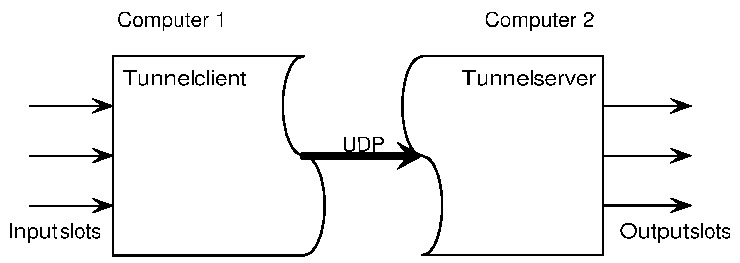
\includegraphics[width=8cm]{pics/tunnel}
%\caption{Tunnel component}
%\label{tunnel_pic}
\end{center}
%\end{figure}

An instance of the tunnel component either represents the input part
(client) or the output part (server). Value changes on the client are
then propagated via UDP datagrams to the server. When creating either
side of the tunnel you have to define the name and type of the slots
that should be created. The slot types of the client and the server
should always match.

\note{ArraySlots are currently not supported.}

\begin{classdesc}{Tunnel}{name = "Tunnel",\\ 
			  server = False, \\
                          slots = None, \\
                          port = 64738, \\
                          host = "localhost", \\
			  gather_messages = False, \\
                          verbose = False, \\
                          auto_insert = True}

\var{server} determines which end of the tunnel is created. The server is
always the ``end'' of a tunnel, i.e. where the values leave the
tunnel.  

\var{slots} specifies the slots to create on the tunnel. It
must be a list of 2-tuples containing two strings. The first string is
the name of the attribute and the second contains the type and
initializer of the slot (in Python syntax). The order and types of the
slots on the client and server should always match.  

\var{port} is the port number to use for the data transfer. The server
listens on this port and the client sends its data to this port on the
target machine.

\var{host} is a string containing the name or IP address of the target
machine where the server part of the tunnel is located. This parameter
is only used on the client side.

\var{gather_messages} determines whether value change messages should be
gathered and sent as one single message or not. If this flag is \code{False},
a message will be sent to the server whenever the value of a slot changes.
However, sometimes it may be the case that you can guarantee that all slots
will change their value at the same time. In such cases, you can set 
\var{gather_messages} to \code{True} which will have the effect that all
messages are collected and delayed until the {\em last} slot receives its 
new value. Only then will the value changes be sent as one big message
which increases the network performance.

If you set \var{verbose} to \code{True} the component will print some
messages so you can follow what it is doing.

\end{classdesc}


Here is an example of a sphere whose position is controlled by a remote
machine:

\begin{verbatim}
# Server code (machine A):

# Create a sphere...
s = Sphere()

# ...and the end of a tunnel that has one Vec3Slot called "pos"
t = Tunnel(
    server = True,
    slots = [("pos", "Vec3Slot()")]
)

# Connect the tunnel slot with the position of the sphere
t.pos_slot.connect(s.pos_slot)
\end{verbatim}

Execute this script with the viewer tool on machine A:

\begin{verbatim}
viewer.py server.py
\end{verbatim}

On the remote machine (the client) you can set the position of the above
sphere with the following code:

\begin{verbatim}
# Client code (machine B):

from cgkit import *

# Create the "entrance" of the tunnel...
t = Tunnel(
    slots = [("pos", "Vec3Slot()")],
    host = "<name or IP of machine A>"
)

# Move the sphere to position (1,0,0)
t.pos_slot.setValue(vec3(1,0,0))
\end{verbatim}

You can call this script by invoking it directly on machine B:

\begin{verbatim}
python client.py
\end{verbatim}

Calling the client code will move the sphere in the first program to 
the position (1,0,0). 

\begin{notice}[note]
As the underlying transport mechanism is using UDP datagrams there is no
error reporting mechanism. The client has no chance of knowing whether
a value change was properly propagated to the server or not. So if you
encounter any problems such as the sphere in the above example {\em not}
moving to another position, you can set the \var{verbose} flag to \code{True}
and additionally check the following points:

\begin{itemize}
\item Do the port numbers on the client and server match?
\item Did you specify the correct host name (or IP address) on the client side?
\item Is there a firewall blocking the network traffic?
\item Did you set \var{gather_messages} to \code{True} and the last slot 
  does not receive any new values? (try to set \var{gather_messages} to
  \code{False})
\end{itemize}

\end{notice}

% ODEDynamics component

\section{\class{ODEDynamics} ---
         Rigid body dynamics using the Open Dynamics Engine}

\begin{classdesc}{ODEDynamics}{name = "ODEDynamics",\\ 
			       gravity = 9.81, \\
                               substeps = 1, \\
                               enabled = True, \\
                               erp = None, \\
                               cfm = None, \\
                               defaultcontactproperties = None, \\
                               collision_events = False, \\
                               auto_add = False, \\
                               show_contacts = False, \\
                               contactmarkersize = 0.1, \\
                               contactnormalsize = 1.0, \\
                               auto_insert = True}

\var{gravity} is the acceleration due to gravity. The direction of the
acceleration is in negative "up" direction (as specified by the scene).

\var{substeps} is the number of simulation steps per frame. You can
increase this value to get a more accurate/stable simulation.

The simulation will only run if \var{enabled} is \code{True}, otherwise
it's halted.

\var{erp} and \var{cfm} are the global error reduction parameter and
constraint force mixing value to be useed (see the ODE manual).

\var{defaultcontactproperties} is a \class{ODEContactProperties} object
that specifies the default contact parameters. These parameters are
used for contacts between two objects (resp. materials) that have not
been set explicitly using \method{setContactProperties()}.

\var{collision_events} determines whether the component will generate
\code{ODE_COLLISION} events whenever a collision has occured. An event
handler takes a \class{ODECollisionEvent} (see section 
\ref{odecollisionevent}) object as argument.

If \var{auto_add} is \code{True} the component searches the scene for
rigid bodies and hinges and adds them automatically to the component.
This is done at the time the component is created, so any bodies or
hinges created afterwards will be ignored.

\var{show_contacts} determines whether the contact points and normals
are visualized or not (this is mainly for debugging purposes).
The size of the contact point markers and the length of the normals
can be specified via the \var{contactmarkersize} and \var{contactnormalsize}
arguments.
\end{classdesc}

\begin{methoddesc}{add}{objects, categorybits=None, collidebits=None}
Add world objects to the simulation. \var{objects} can be a single
object or a sequence of objects. An object may be specified by its
name or the object itself. \var{categorybits} and \var{collidebits}
are long values that control which objects can collide with which
other object. The specified category and collide bits are assigned to every
object in \var{objects}. Each bit in \var{categorybits} represents
one category the objects belong to. \var{collidebits} is another bit
field that specifies with which categories the objects may collide.
By default, every bit is set in both values.
\end{methoddesc}

\begin{methoddesc}{reset}{}
Reset the state of the simulated bodies. All bodies will be set to the
position and velocity they had when they were added to the simulation.
This method is also called when the RESET event is issued.
\end{methoddesc}

\begin{methoddesc}{setContactProperties}{(mat1, mat2), props}
Set the contact properties for a material pair. \var{mat1} and \var{mat2}
are two \class{Material} objects and props is a \class{ODEContactProperties}
object describing the contact properties.
\end{methoddesc}

\begin{methoddesc}{getContactProperties}{(mat1, mat2)}
Return the contact properties for a material pair. The order of the materials
is irrelevant. The return value is
a \class{ODEContactProperties} object. A default property object is
returned if the pair does not have any properties set.
\end{methoddesc}

\begin{methoddesc}{createBodyManipulator}{object}
Return an \class{ODEBodyManipulator} object that can be used to apply
external forces/torques to the world object \var{object}.
\end{methoddesc}


\begin{notice}[note]
To use the \class{ODEDynamics} component the
\ulink{PyODE}{http://pyode.sourceforge.net/} module has to be 
installed on your system which wraps the 
\ulink{Open Dynamics Engine}{http://www.ode.org/}.
\end{notice}

%------------------------------------------------------
\subsection{\class{ODEContactProperties} ---
         Contact properties during collision}

The \class{ODEContactProperties} class contains all the parameters
that are used when two objects collide. 

\begin{classdesc}{ODEContactProperties}{mode = 0,\\
			       mu = 0.3,\\
			       mu2 = None,\\
			       bounce = None,\\
			       bounce_vel = None,\\
			       soft_erp = None,\\
			       soft_cfm = None,\\
			       motion1 = None,\\
			       motion2 = None,\\
			       slip1 = None,\\
			       slip2 = None,\\
			       fdir1 = None}

See the ODE manual (chapter 
\ulink{7.3.7 {\em Contact}}{http://ode.org/ode-latest-userguide.html#sec_7_3_7})
for an explanation of these
parameters.

\note{You only have to specify the \var{mode} argument if you want to set
the ContactApprox* flags. The other flags are automatically set.}
\end{classdesc}

%------------------------------------------------------
\subsection{\class{ODEBodyManipulator} ---
         Apply external forces/torques to bodies}

The \class{ODEBodyManipulator} class can be used to apply external
forces and torques to a rigid body. 

\begin{classdesc*}{ODEBodyManipulator}
You get an instance of this class
by calling the
\method{createBodyManipulator()} method of the \class{ODEDynamics} component.
One particular body manipulator instance is always associated with one
particular rigid body. A manipulator object has the following attributes
and methods:
\end{classdesc*}

\begin{memberdesc}{body}
This attribute contains the rigid body (\class{WorldObject}) this
manipulator is associated with. You can only read this attribute. If
you want to control another body, use the
\method{createBodyManipulator()} method of the dynamics component.
\end{memberdesc}

\begin{memberdesc}{odebody}
This is the Body instance of the PyODE module. You can use this object
if you want to access special features of ODE that are not exposed otherwise.
But note that you won't get the expected results if you call methods like
\method{addForce()} directly on the ODE body and you're using more than
one sub step in your simulation. The force would only be applied during
the first sub step because it is reset after each step. Use this
manipulator class instead, that's what it's for.
\end{memberdesc}

% addForce
\begin{methoddesc}{addForce}{force, relforce=False, pos=None, relpos=False}
Add an external force to the current force vector. \var{force} is a vector
containing the force to apply. If \var{relforce} is \code{True} the force
is interpreted in local object space, otherwise it is assumed to be given
in global world space. By default, the force is applied at the center
of gravity. You can also pass a different position in the \var{pos} argument
which must describe a point in space. \var{relpos} determines if the
point is given in object space or world space (default).
\end{methoddesc}

% addTorque
\begin{methoddesc}{addTorque}{torque, reltorque=False}
Add an external torque to the current torque vector. \var{torque} is
a vector containing the torque to apply. \var{reltorque} determines if
the torque vector is given in object space or world space (default).
\end{methoddesc}

% setInitialPos
\begin{methoddesc}{setInitialPos}{pos}
Set the initial position of the body. \var{pos} must be a 3-sequence of 
floats containing the new position.
\end{methoddesc}

% setInitialRot
\begin{methoddesc}{setInitialRot}{rot}
Set the initial orientation of the body. \var{rot} must be a
\class{mat3} containing a rotation matrix.
\end{methoddesc}

% setInitialLinearVel
\begin{methoddesc}{setLinearVel}{vel}
Set the initial linear velocity of the body. \var{vel} must be a
3-sequence of floats containing the new velocity.
\end{methoddesc}

% setInitialAngularVel
\begin{methoddesc}{setAngularVel}{vel}
Set the initial angular velocity of the body. \var{vel} must be a
3-sequence of floats containing the new velocity.
\end{methoddesc}

% setPos
\begin{methoddesc}{setPos}{pos}
Set the position of the body. \var{pos} must be a 3-sequence of floats
containing the new position.
\end{methoddesc}

% setRot
\begin{methoddesc}{setRot}{rot}
Set the orientation of the body. \var{rot} must be a \class{mat3} containing a
rotation matrix.
\end{methoddesc}

% setLinearVel
\begin{methoddesc}{setLinearVel}{vel}
Set the linear velocity of the body. \var{vel} must be a 3-sequence of floats
containing the new velocity.
\end{methoddesc}

% setAngularVel
\begin{methoddesc}{setAngularVel}{vel}
Set the angular velocity of the body. \var{vel} must be a 3-sequence of floats
containing the new velocity.
\end{methoddesc}

%------------------------------------------------------
\subsection{\class{ODECollisionEvent} ---
         Collision event object}
\label{odecollisionevent}

An \class{ODECollisionEvent} object is passed as argument to the event
handler for \code{ODE_COLLISION} events.

\begin{classdesc}{ODECollisionEvent}{obj1, obj2, contacts, contactproperties}

\var{obj1} and \var{obj2} are the two world objects that have collided with 
each other.

\var{contacts} is a list of \class{ode.Contact} objects that each describes
a contact point.

\var{contactproperties} is a \class{ODEContactProperties} object that
describes the properties of the contact. It depends on the materials
of the \var{obj1} and \var{obj2}. The event handler may modify
this object to change the result of the collision. Note however, that
the changes will be permanent and also affect later collisions.
\end{classdesc}

% averageContactGeom
\begin{methoddesc}{averageContactGeom}{}
Return the average contact position, normal and penetration depth (in
this order). The position and normal are returned as \class{vec3}
objects, the penetration depth is a float.
\end{methoddesc}

% FlockOfBirds component

\section{\class{FlockOfBirds} ---
         Retrieving values from an Ascension Flock of Birds\textsuperscript{\textregistered} motion tracker}

The \class{FlockOfBirds} class communicates with an Ascension Flock
of Birds\textsuperscript{\textregistered} motion tracker 
(\url{http://www.ascension-tech.com/}) via the serial port and provides the 
sensor values of the individual birds via slots.

Note: Currently, the class assumes that an extended range controller is
used! (this means the position values have to be adjusted if you use the
tracker without an extended range controller)

\begin{classdesc}{FlockOfBirds}{name = "FlockOfBirds",\\ 
                                com_port = 0,\\
                                baud_rate = 115200,\\
                                timeout = 2.0,\\
                                num_birds = 1,\\
                                bird_mode = "p",\\
                                hemisphere = "forward",\\
                                auto_insert = True}


\var{com_port} specifies which COM port to use for the communication with
the flock (0-based port number).

\var{baud_rate} is the baud rate to use.

\var{timeout} specifies a time span in seconds after which a RS232 operation
fails.

\var{num_birds} is the number of birds to use (including the ERC which will 
be bird 1).

\var{bird_mode} selects what kind of data the birds will send. It can be either
a string containing the mode for all birds or it can be a list of strings
to select a mode for each individual bird. In the latter case, the list must
hold one string for each bird. The mode string can be one of the values
in the following table:

\begin{tableii}{c|l}{code}{Mode}{Description}
\lineii{"p"}{Send only the position.}
\lineii{"a"}{Send only euler angles.}
\lineii{"m"}{Send only a rotation matrix.}
\lineii{"q"}{Send only a quaternion.}
\lineii{"pa"}{Send position and euler angles.}
\lineii{"pm"}{Send position and matrix.}
\lineii{"pq"}{Send position and quaternion.}
\end{tableii}

\var{hemisphere} specifies in which hemisphere, centered about the
transmitter, the sensor will be operating (see the {\em Flock of Birds ---
Installation and Operation Guide}). The values can be one of \code{"forward"},
\code{"aft"}, \code{"upper"}, \code{"lower"}, \code{"left"} and \code{"right"}.

\end{classdesc}


For each bird, the \class{FlockOfBirds} component creates the following
four slots:

\begin{itemize}
\item \code{pos<n>_slot} (\code{Vec3Slot}) -- Position (in cm)
\item \code{angle<n>_slot} (\code{Vec3Slot}) -- Euler angles
\item \code{matrix<n>_slot} (\code{Mat3Slot}) -- Rotation matrix
\item \code{quat<n>_slot} (\code{QuatSlot}) -- Quaternion
\end{itemize}

where \code{<n>} is the number of the bird (1-based). Not all of the
slots are active at the same time. You can select which slot should
carry the corresponding value via the bird mode.

\begin{notice}[note]
To use the \class{FlockOfBirds} component the
\ulink{pySerial}{http://pyserial.sourceforge.net/} module has to be 
installed on your system.
\end{notice}


% GnuPlotter component

\section{\class{GnuPlotter} ---
         Plot values using Gnuplot}

The \class{GnuPlotter} class can be used to plot the graph of a
floating point slot. To do so, connect any \class{DoubleSlot} to
an input slot of the plotter. The input slots are called \code{input<n>_slot}
where \code{<n>} is the number of the slot.

\begin{classdesc}{GnuPlotter}{name = "GnuPlotter",\\ 
                              title = None, \\
                              xlabel = None, \\
                              ylabel = None, \\
                              xrange = None, \\
                              yrange = None, \\
                              inputs = 1, \\
                              plottitles = [], \\
                              starttime = 0.0, \\
                              endtime = 99999.0, \\
                              enabled = True, \\
                              auto_insert = True}

\var{title} is a string containing the title of the entire plot.

\var{xlabel}, \var{ylabel} are strings containing the labels for the X and
Y axis.

\var{xrange}, \var{yrange} is each a 2-tuple (\var{start}, \var{end}) 
containing the range of the X axis resp. Y axis.

\var{inputs} is the number of input slots that should be created (i.e.
the number of curves you want to plot).

\var{plottitles} is a list of strings containing the name of the respective
curve.

\var{starttime} and \var{endtime} defines the range in which values are
received and plotted. The times are given in seconds.

\var{enabled} is a flag that can be used to disable the plotter.
\end{classdesc}

A \class{GnuPlotter} object has the following slots:

\begin{tableiv}{l|l|c|l}{code}{Slot}{Type}{Access}{Description}
\lineiv{input1_slot}{float}{rw}{First curve}
\lineiv{input2_slot}{float}{rw}{Second curve}
\lineiv{...}{...}{...}{...}
\end{tableiv}

% --------------------
\begin{notice}[note]
To use the \class{GnuPlotter} component the
\ulink{Gnuplot.py}{http://gnuplot-py.sourceforge.net/} module has to be 
installed on your system (and of course, 
\ulink{gnuplot}{http://www.gnuplot.info/} itself as well).
\end{notice}


% PIDController component

\section{\class{PIDController} ---
         Proportional-Integral-Derivative controller}

A PID controller is a standard component in industrial control
applications which tries to keep a measured value at a given target
value (the {\em setpoint}). The measured value has to be plugged into
the input slot (\code{input_slot}) and the output of the PID controller
can be read from \code{output_slot}.

%\begin{displaymath}
%output(t) = K_p \cdot err(t) + K_i \cdot \int err(t')\, dt' + K_d \cdot \frac{d\,err}{dt}
%\end{displaymath}

For example, you can use a PID controller in conjunction with the
joints in the \class{ODEDynamics} component to keep a hinge or slider
at a particular position. In this case the angle or position is used
as input to the PID controller and the output controls the motor velocity.

\begin{classdesc}{PIDController}{name = "PIDController",\\ 
                              setpoint = 0.0, \\
                              Kp = 0.0, \\
                              Ki = 0.0, \\
                              Kd = 0.0, \\
                              maxout = 999999, \\
                              minout = -999999, \\
                              auto_insert = True}

\var{setpoint} is the target value that should be maintained.

\var{Kp} is the weight for the proportional part, \var{Ki} the weight
for the integral part and \var{Kd} the weight for the derivative part.

\var{maxout} and \var{minout} are used to clamp the output value.
\end{classdesc}

A \class{PIDController} has the following slots:

\begin{tableiv}{l|l|c|l}{code}{Slot}{Type}{Access}{Description}
\lineiv{input_slot}{float}{rw}{The "measured" value}
\lineiv{setpoint_slot}{float}{rw}{The target value}
\lineiv{output_slot}{float}{r}{Controller output}
\lineiv{maxout_slot}{float}{rw}{Maximum output value}
\lineiv{minout_slot}{float}{rw}{Minimum output value}
\lineiv{Kp_slot}{float}{rw}{Weight for the proportional term}
\lineiv{Ki_slot}{float}{rw}{Weight for the integral term}
\lineiv{Kd_slot}{float}{rw}{Weight for the derivative term}
\end{tableiv}




% SlideShow component

\section{\class{SlideShow} ---
         Displaying a series of images}

The \class{SlideShow} class can be used to display image files as
a slide show. The component sets up a scene and displays an image
sequence with user defined transitions.

\begin{classdesc}{SlideShow}{name = "SlideShow",\\ 
                             slides = [], \\
                             auto_insert = True}

\var{slides} is either a string specifying the image files (the string
may contain wildcards) or a list of \class{Slide} objects where each
object represents one or more images.
\end{classdesc}

Example:

\begin{verbatim}
# File: slides.py

SlideShow(
    slides = [
              Slide("image01.jpg", XFade(1.0) ),
              Slide("image02.jpg", XFade(1.0, 0.3) ),
              Slide("image03.jpg", XCube(2.0) ),
              Slide("presentation/slides*.png", XFade(0.5) )
             ]
)
\end{verbatim}

The slide show is started with the viewer tool like this:

\begin{verbatim}
viewer.py slides.py -f50 -F
\end{verbatim}

In this case, the frame rate is increased to 50 frames per second (to get
smoother transitions) and the display is set to full screen.

When the slide show is running you can jump to the next slide by pressing
a mouse button, the \kbd{Enter} key or the \kbd{PageDown} key.
In case you move the camera, you can reset it with the \kbd{q} key.

%----------------------------------------------------------------------
\subsection{Slide class}

The \class{Slide} class represents one or more image files and contains
one transition that is used for all files.

\begin{classdesc}{Slide}{filepattern, transition = XCube()}

\var{filepattern} specifies the image files to load and may include
wildcards to select more than one file.

\var{transition} is a transition class that determines the transition
that is applied after each image in this slide object.
\end{classdesc}

%----------------------------------------------------------------------
\subsection{XFade transition}

The \class{XFade} transition implements a smooth cross fade between two
images.

\begin{classdesc}{XFade}{duration=2.0, zmove=0.0}

\var{duration} is the length of the transition in seconds.

If \var{zmove} is greater than 0, the old image will be moved towards
the camera during the transition which makes it scale up when viewed
with a perspective camera.
\end{classdesc}

%----------------------------------------------------------------------
\subsection{XCube transition}

The \class{XCube} class implements a transition where the images seem
to be attached on two adjacent sides of a cube and the cube rotates
during the transition.

\begin{classdesc}{XCube}{duration=2.0}

\var{duration} is the length of the transition in seconds.
\end{classdesc}


% MotionPath

\section{\class{MotionPath} ---
         Motion path}

\begin{classdesc}{MotionPath}{name = "MotionPath",\\ 
                              curve = None,\\
                              begintime = 0.0,\\
                              endtime = 1.0,\\
                              loop = False,\\
                              follow = False,\\
                              bank = False,\\
                              bankamplitude = 0.1,\\
                             }

\var{curve} is an object supporting the curve protocol.

\var{begintime} and \var{endtime} specify the parameter interval of
the motion. At \var{begintime} the object will be located at the beginning
of the curve and at \var{endtime} it will be at the end.

\var{loop} is a boolean that specifies if the motion is repeated when 
outside the specified parameter interval.

\var{follow} determines if the object will change its orientation to
follow the path.

\var{bank} determines if the object will roll if the curve makes a turn.
\var{bankamplitude} specifies how much the obect will roll.

\end{classdesc}




%---
\chapter{WorldObjects \label{worldobjects}}

% WorldObject

\section{\class{WorldObject} ---
         World object base class}

\begin{classdesc}{WorldObject}{name = "object", \\
                 transform = None,\\
                 pos = None, \\
	         rot = None,\\
                 scale = None,\\
                 pivot = None,\\
                 offsetTransform = None,\\
                 parent = None,\\
                 mass = None,\\
                 material = None,\\
                 visible = True,\\
                 auto_insert = True}

\var{name} is the name of the object which can be used to identify the
object.

\var{transform} is the initial transformation that should be applied to
the object. Alternatively, you can specify the individual components
\var{pos}, \var{rot} and \var{scale}.

\var{pivot} is the pivot point of the object. This is the 4th column of
the offset transformation. You can also specify the entire offset 
transformation using the \var{offsetTransform} argument.

\var{parent} is the parent world object and determines at which position
in the scene graph the new object is added. If \var{parent} is \code{None}
the object will become a child of the world root. The \var{parent} argument
is only used if \var{auto_insert} is \code{True}.

\var{mass} is the mass of this object (this does {\em not} include
the children objects).

\var{material} describes the appearance of the object. It can be either 
a single \class{Material} object or a sequence of \class{Material} objects.

\var{visible} is a flag that determines whether the object is visible
or not. This only affects the geometry of this WorldObject, it is not
inherited by children objects.

The object will be inserted into the scene automatically if 
\var{auto_insert} is set to \code{True}.
\end{classdesc}

A \class{WorldObject} always has the following slots:

\begin{tableiv}{l|l|c|l}{code}{Slot}{Type}{Access}{Description}
\lineiv{angularvel_slot}{vec3}{rw}{Angular velocity}
\lineiv{cog_slot}{vec3}{r}{Center of gravity}
\lineiv{inertiatensor_slot}{mat3}{r}{Inertia tensor}
\lineiv{linearvel_slot}{vec3}{rw}{Linear velocity}
\lineiv{mass_slot}{float}{rw}{Mass of the local geometry}
\lineiv{pos_slot}{vec3}{rw}{Position}
\lineiv{rot_slot}{mat3}{rw}{Orientation}
\lineiv{scale_slot}{vec3}{rw}{Scaling}
\lineiv{totalmass_slot}{float}{r}{Total mass (including the children)}
\lineiv{transform_slot}{mat4}{rw}{Object transformation}
\lineiv{visible_slot}{bool}{rw}{Visibility flag}
\lineiv{worldtransform_slot}{mat4}{rw}{World transformation}
\end{tableiv}

\begin{memberdesc}{geom}
This attribute holds the visible geometry which must be derived from 
\class{GeomObject}. The value can also be \code{None} if there is no
visible geometry. Geometry objects can be shared between different 
world objects. This value can be read and written.
\end{memberdesc}

\begin{memberdesc}{parent}
This attribute contains the parent world object or \code{None}. You can 
only read this attribute.
\end{memberdesc}

\begin{memberdesc}{transform}
This is the value of the mat4 slot \var{transform_slot} which contains
the object transformation T. You can read and write this attribute.
\end{memberdesc}

\begin{memberdesc}{worldtransform}
This is the value of the mat4 slot \var{worldtransform_slot} which
contains the world transformation (which is a concatenation of all local
transformations L). You can only read this attribute.

\note{Note that in contrast to the \var{transform} slot,
the \var{worldtransform} is not influenced by the offset transformation.}
\end{memberdesc}

\begin{memberdesc}{pos}
This is the value of the vec3 slot \var{pos_slot} which contains the 
position of the object. You can read and write this attribute.
\end{memberdesc}

\begin{memberdesc}{rot}
This is the value of the mat3 slot \var{rot_slot} which contains the 
orientation of the object. You can read and write this attribute.
\end{memberdesc}

\begin{memberdesc}{scale}
This is the value of the vec3 slot \var{scale_slot} which contains the 
scaling of the object. You can read and write this attribute.
\end{memberdesc}

\begin{memberdesc}{pivot}
This is the pivot point (vec3) of the object. You can read and write this
attribute. Reading or writing this attribute is equivalent to calling
\method{getOffsetTransform()} or \method{setOffsetTransform()} with
a matrix that only modifies the 4th column.
\end{memberdesc}

\begin{memberdesc}{cog}
This is the value of the vec3 slot \var{cog_slot} which contains the
physical center of gravity. This value is derived from the center of 
gravity provided by the geometry object and the cogs and masses of the
children objects. This means it represents the center of gravity of the 
entire hierarchy. The value is given with respect to the pivot coordinate
system P. You can only read this value.
\end{memberdesc}

\begin{memberdesc}{inertiatensor}
This is the value of the mat3 slot \var{inertiatensor_slot} which contains
the inertia tensor of the entire hierarchy (just like \var{cog}). You can
only read this value.
\end{memberdesc}

\begin{memberdesc}{mass}
This is the value of the double slot \var{mass_slot} which contains the
{\em local} mass of this object (not including the children). Or in other
words, this is the mass of the geometry directly set in this object.
You can read and write this value.
\end{memberdesc}

\begin{memberdesc}{totalmass}
This is the value of the double slot \var{totalmass_slot} which contains
the total mass of this object and its children. You can only read this value.
\end{memberdesc}

\begin{memberdesc}{angularvel}
This is the value of the vec3 slot \var{angular_slot} which contains the 
angular velocity of the object. The value is not computed but has to be
set by anyone who knows the angular velocity (such as a dynamics component).
You can read and write this attribute.
\end{memberdesc}

\begin{memberdesc}{linearvel}
This is the value of the vec3 slot \var{linearvel_slot} which contains the 
linear velocity of the object. The value is not computed but has to be
set by anyone who knows the linear velocity (such as a dynamics component).
You can read and write this attribute.
\end{memberdesc}


% Methods
\begin{methoddesc}{boundingBox}{}
Return the local axis aligned bounding box. The bounding box is
given with respect to the local transformation L (which is not
what you get from the transform slot of the world object).
\end{methoddesc}

\begin{methoddesc}{localTransform}{}
Returns the local transformation that has to be used for rendering.
The returned transformation L is calculated as follows: $L = T\cdot P^{-1}$,
where T is the current transform (taken from the transform slot)
and P is the offset transform.
\end{methoddesc}

\begin{methoddesc}{getOffsetTransform}{}
Return the current offset transformation as a \class{mat4}. This
transformation is given relative to the local object transformation.
\end{methoddesc}

\begin{methoddesc}{setOffsetTransform}{P}
Set the offset transformation. The transformation has to be given
relative to the local object transformation. After setting the offset
transformation, the transform slot will be updated so that 
\method{localTransform()} returns the same matrix as before, i.e. the
world position/orientation of the object does not change.
\end{methoddesc}

\begin{methoddesc}{getNumMaterials}{}
Return the current size of the material array.
\end{methoddesc}

\begin{methoddesc}{setNumMaterials}{num}
Set a new size for the material array.
\end{methoddesc}

\begin{methoddesc}{getMaterial}{idx=0}
Get a stored material. The method returns \code{None} if the given index
is out of range or there is no material stored at that position.
\end{methoddesc}

\begin{methoddesc}{setMaterial}{mat, idx=0}
Set a new material. An \exception{IndexError} exception is thrown if
the index is out of range.
\end{methoddesc}

\begin{methoddesc}{lenChilds}{}
Return the number of children objects.
\end{methoddesc}

\begin{methoddesc}{iterChilds}{}
Return an iterator that iterates over all children objects.
\end{methoddesc}

\begin{methoddesc}{hasChild}{name}
Check if a children with a particular name does exist.
\end{methoddesc}

\begin{methoddesc}{child}{name}
Return the children with a particluar name. A \exception{KeyError}
exception is thrown if there is no children with the specified name.
\end{methoddesc}

\begin{methoddesc}{addChild}{child}
Add a new children world object to this object. A
\exception{ValueError} exception is thrown if child was already added
to another object.  In this case you have to remove the object from
its previous parent yourself. You also have to make sure that the name
of \var{child} is unique among the children of this object, otherwise
a \exception{KeyError} exception is thrown.
\end{methoddesc}

\begin{methoddesc}{removeChild}{child}
Remove a children world object from this object. \var{child} can either
be the name of the children or the object itself. A \exception{KeyError}
exception is thrown if child is not a children of this object.
\end{methoddesc}

\begin{methoddesc}{makeChildNameUnique}{name}
Modify \var{name} so that it is unique among the children names. If
\var{name} is already the name of a children object, then it is modified
by adding/increasing a trailing number, otherwise it is returned
unchanged.
\end{methoddesc}





% Box

\section{\class{Box} ---
         Box object}

\begin{classdesc}{Box}{name = "Box",\\ 
                       lx = 1.0,\\
                       ly = 1.0,\\
                       lz = 1.0,\\
                       segmentsx = 1,\\
                       segmentsy = 1,\\
                       segmentsz = 1,\\
%                       transform = None,\\
%                       pos = None,\\
%                       rot = None,\\
%                       scale = None,\\
%                       pivot = None,\\
%                       offsetTransform = None,\\
%                       material = None,\\
%                       mass = None,\\
                       dynamics = True,\\
                       static = False,\\
                       ...[WorldObject params]...
                       }

\end{classdesc}



% Sphere

\section{\class{Sphere} ---
         Sphere object}

\begin{classdesc}{Sphere}{name = "Sphere",\\ 
                       radius = 1.0,\\
                       segmentsu = 16,\\
                       segmentsv = 8,\\
%                       transform = None,\\
%                       pos = None,\\
%                       rot = None,\\
%                       scale = None,\\
%                       pivot = None,\\
%                       offsetTransform = None,\\
%                       material = None,\\
%                       mass = None,\\
                       dynamics = True,\\
                       static = False,\\
%                       auto_insert = True\\
                       ...[WorldObject params]...
		       }

\end{classdesc}



% Capped Cylinder

\section{\class{CCylinder} ---
         Capped cylinder object}

\begin{classdesc}{CCylinder}{name = ''CCylinder'',\\ 
                       radius = 1.0,\\
                       length = 1.0,\\
                       segmentsu = 16,\\
                       segmentsvl = 1,\\
                       segmentsvr = 4,\\
%                       transform = None,\\
%                       pos = None,\\
%                       rot = None,\\
%                       scale = None,\\
%                       pivot = None,\\
%                       offsetTransform = None,\\
%                       material = None,\\
%                       mass = None,\\
                       dynamics = True,\\
                       static = False,\\
                       ...[WorldObject params]...
                       }

\end{classdesc}



% Plane

\section{\class{Plane} ---
         Plane object}

\begin{classdesc}{Plane}{name = ''Plane'',\\ 
                       lx = 1.0,\\
                       ly = 1.0,\\
                       segmentsx = 1,\\
                       segmentsy = 1,\\
                       transform = None,\\
                       pos = None,\\
                       rot = None,\\
                       scale = None,\\
                       pivot = None,\\
                       offsetTransform = None,\\
                       material = None,\\
                       mass = None,\\
                       dynamics = True,\\
                       auto_insert = True}

\end{classdesc}



% Torus

\section{\class{Torus} ---
         Torus object}

\begin{classdesc}{Torus}{name = "Torus",\\ 
                         major = 1.0,\\
                         minor = 0.1,\\
                         segmentsu = 16,\\
                         segmentsv = 8,\\
                         ...[WorldObject params]...
	   	       }

\end{classdesc}



% TriMesh

\section{\class{TriMesh} ---
         Triangle mesh object}

\begin{classdesc}{TriMesh}{name = ''TriMesh'',\\ 
                       verts = [],\\
                       faces = [],\\
                       transform = None,\\
                       pos = None,\\
                       rot = None,\\
                       scale = None,\\
                       pivot = None,\\
                       offsetTransform = None,\\
                       material = None,\\
                       mass = None,\\
                       dynamics = True,\\
                       static = False,\\
                       auto_insert = True}

\end{classdesc}



% Polyhedron

\section{\class{Polyhedron} ---
         Polyhedron object}

\begin{classdesc}{Polyhedron}{name = "Polyhedron",\\ 
                              verts = [],\\
                              polys = []
			     }	

\end{classdesc}



% Group

\section{\class{Group} ---
         Group object}

\begin{classdesc}{Group}{name = ''Group'',\\ 
                       childs = [],\\
                       transform = None,\\
                       pos = None,\\
                       rot = None,\\
                       scale = None,\\
                       pivot = None,\\
                       offsetTransform = None,\\
                       dynamics = True,\\
                       static = False,\\
                       auto_insert = True}

\end{classdesc}



% Joint

\section{\class{Joint} ---
         Joint class for creating a skeleton}

The \class{Joint} class can be used to create articulated
characters. Bones are implicitely created by linking two joints, i.e.
a bone is assumed between a joint and each of its children joints.
A \class{Joint} object corresponds to a ball joint that has three rotational
degrees of freedom. The actual joint is always located at the pivot point
of the \class{Joint} object and rotates about the pivot frame axes.

If you want your local coordinate frame to be oriented differently, it
is not enough to set the offset transform as this will also readjust the
local frame so that the effect is actually cancelled out and you will
still rotate about the same axes as before. To initialize the new frame
you have to call \method{freezePivot()} after setting the offset transform.
This will set the current offset transform as the new default pose where
all angles are 0 and will make the joint rotate about the new axes.
After freezing you may want to set the offset transform back to the identity
so that the local coordinate frame and the offset frame coincide again.
This won't affect the rotation of the joint but the location of its
children (as setting the offset transform on a \var{Joint} object also
modifies its local coordinate system). But it actually depends on the
situation whether you have to reset the offset transform or not.

Rotating a joint is not done by setting its \var{rot} attribute but
by setting its three individual angles (\var{anglex}, \var{angley}, 
\var{anglez}).

\begin{classdesc}{Joint}{name = "", \\
			 radius = 0.05, \\
	                 rotationorder = "xyz"
		         }

\var{name} is the name of the joint.

\var{radius} is the radius of the visual representation of the joint/bone.

\var{rotationorder} determines the order of rotation about the individual
axes.
\end{classdesc}

A \class{Joint} has the following slots:

\begin{tableiv}{l|l|c|l}{code}{Slot}{Type}{Access}{Description}
\lineiv{anglex_slot}{float}{rw}{Angle around x axis}
\lineiv{angley_slot}{float}{rw}{Angle around y axis}
\lineiv{anglez_slot}{float}{rw}{Angle around z axis}
\end{tableiv}

\begin{memberdesc}{anglex}
Rotation angle (in degrees) about the local x axis.
\end{memberdesc}

\begin{memberdesc}{angley}
Rotation angle (in degrees) about the local y axis.
\end{memberdesc}

\begin{memberdesc}{anglez}
Rotation angle (in degrees) about the local z axis.
\end{memberdesc}

% Methods
\begin{methoddesc}{freezePivot}{}
Make the current pivot coordinate system the default pose. After
calling this method, the current rotation of the pivot coordinate
system will define the default pose. This means, rotations are now
defined around the local pivot axes. 
\end{methoddesc}







% TargetCamera

\section{\class{TargetCamera} ---
         Target camera}

The \class{TargetCamera} class always looks at a specified point and
aligns its local up direction to the scene up direction.

\begin{classdesc}{TargetCamera}{name = "TargetCamera",\\ 
                       target = (0,0,0),\\
                       fov = 45.0,\\
                       roll = 0.0, \\
                       up = None,\\
                       focallength = 0,\\
                       fstop = 0,\\
                       auto_nearfar = True,\\
                       nearplane = 0.1,\\
                       farplane = 1000.0,\\
                       }

\var{target} is the point that the camera will always look at. 

\var{fov} is the field of view in degrees (in vertical direction), i.e.
the angle between the bottom and the top of the screen.

\var{roll} is an angle in degrees that the camera is rotated about its 
local z axis.

\var{up} is the vector that is considered to be the 'up' direction. If
\code{None} is passed, the global 'up' direction from the scene is used.

\var{focallength} is the focal length of the camera and \var{fstop} the
aperture number that determines the lens diameter. These values are used
to turn on depth of field. Depth of field is activated if both attributes
are set to a value different from 0 (note however, that not every renderer
supports depth of field). The focal distance is set so that the target 
point will always be in focus.

\var{auto_nearfar} specifies whether the near and far plane
distances are automatically determined or if fixed values are used.
If set to \code{False}, the \var{nearplane} and \var{farplane} arguments
are used, otherwise the values are computed from the objects in the scene.
In the latter case, the \var{nearplane} value still serves as minimum
value for the near plane distance which is used when the camera is located
within the scene bounds.
\end{classdesc}

The \class{TargetCamera} has the following slots (in addition to the slots
of the \class{WorldObject} base class):

\begin{tableiv}{l|l|c|l}{code}{Slot}{Type}{Access}{Description}
\lineiv{target_slot}{vec3}{rw}{Target point}
\lineiv{fov_slot}{float}{rw}{Field of view in degrees}
\lineiv{roll_slot}{float}{rw}{Rotation about local z axis (in degrees)}
\lineiv{up_slot}{vec3}{rw}{Up direction}
\lineiv{focallength_slot}{float}{rw}{Focal length of the camera}
\lineiv{fstop_slot}{float}{rw}{Aperture number}
\lineiv{autonearfar_slot}{bool}{rw}{Automatically compute near/far values?}
\lineiv{nearplane_slot}{float}{rw}{(Minimal) near plane distance}
\lineiv{farplane_slot}{float}{rw}{Far plane distance}
\end{tableiv}

\begin{methoddesc}{projection}{width, height, near, far}
Returns the projection matrix for a viewport with the given width and
height (actually only the ratio width/height is relevant). The near
and far clipping planes are set to \var{near} and \var{far}.
\end{methoddesc}

\begin{methoddesc}{viewTransformation}{}
Returns the view transformation for this camera.
\end{methoddesc}

\begin{methoddesc}{eyeRay}{x0, y0, width, height}
Return a ray whose origin is at the eye position and that goes through
a given point on the image plane. The point on the plane is given by
(\var{x0}, \var{y0}) which each ranges from 0 to 1. (0,0) is at the
upper left and (1,1) at the lower right corner. The arguments \var{width} and
\var{height} determine the ratio of the image plane (the absolute
values of \var{width} and
\var{height} are irrelevant). The return value is a 2-tuple (\var{p}, \var{u})
where \var{p} is the ray origin and \var{u} the normalized
direction. Both vectors are given in world space.

\begin{center}
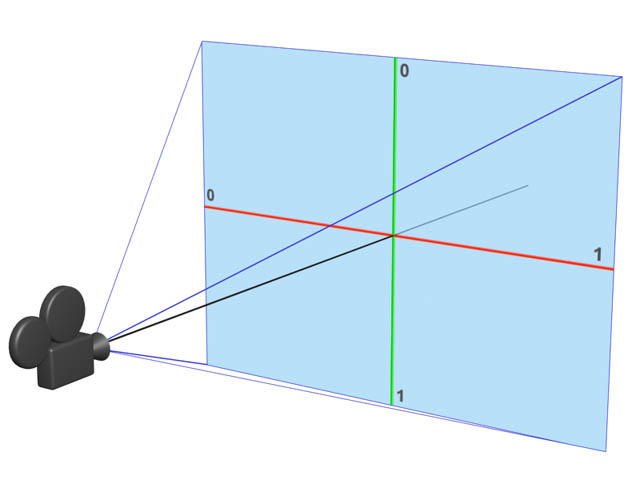
\includegraphics[width=9cm]{pics/camera01}
\end{center}
\end{methoddesc}

\begin{methoddesc}{getNearFar}{}
Return a 2-tuple (\var{near}, \var{far}) with the distances to the
near and far clipping planes. If automatic computation is disabled,
the method just returns the stored values, otherwise the values
are computed from the bounding box of the scene (which is converted
to a bounding sphere and the clipping planes are set as tangent planes
to the sphere).
\end{methoddesc}

% FreeCamera

\section{\class{FreeCamera} ---
         Free camera}

The \class{FreeCamera} class can be freely positioned and oriented in 
the scene.

\begin{classdesc}{FreeCamera}{name = "FreeCamera",\\ 
                       fov = 45.0,\\
                       target = None,\\
                       focallength = 0,\\
                       fstop = 0,\\
                       auto_nearfar = True,\\
                       nearplane = 0.1,\\
                       farplane = 1000.0,\\
                       }

\var{fov} is the field of view in degrees (in vertical direction), i.e.
the angle between the bottom and the top of the screen.

\var{target} is the point that the camera will initially look at. If no
target is specified the camera remains in its default orientation. Note
that the target is only used to compute an initial orientation. The
orientation will not be updated if the camera moves (use a 
\class{TargetCamera} if you want that behavior).

\var{focallength} is the focal length of the camera and \var{fstop} the
aperture number that determines the lens diameter. These values are used
to turn on depth of field. Depth of field is activated if both attributes
are set to a value different from 0 (note however, that not every renderer
supports depth of field). The focal distance is set so that the target 
point will always be in focus.

\var{auto_nearfar} specifies whether the near and far plane
distances are automatically determined or if fixed values are used.
If set to \code{False}, the \var{nearplane} and \var{farplane} arguments
are used, otherwise the values are computed from the objects in the scene.
In the latter case, the \var{nearplane} value still serves as minimum
value for the near plane distance which is used when the camera is located
within the scene bounds.
\end{classdesc}

The \class{FreeCamera} class has the following slots (in addition to
the slots of the \class{WorldObject} base class):

\begin{tableiv}{l|l|c|l}{code}{Slot}{Type}{Access}{Description}
\lineiv{fov_slot}{float}{rw}{Field of view in degrees}
\lineiv{focallength_slot}{float}{rw}{Focal length of the camera}
\lineiv{fstop_slot}{float}{rw}{Aperture number}
\lineiv{autonearfar_slot}{bool}{rw}{Automatically compute near/far values?}
\lineiv{nearplane_slot}{float}{rw}{(Minimal) near plane distance}
\lineiv{farplane_slot}{float}{rw}{Far plane distance}
\end{tableiv}

\begin{methoddesc}{projection}{width, height, near, far}
Returns the projection matrix for a viewport with the given width and
height (actually only the ratio width/height is relevant). The near
and far clipping planes are set to \var{near} and \var{far}.
\end{methoddesc}

\begin{methoddesc}{viewTransformation}{}
Returns the view transformation for this camera.
\end{methoddesc}

\begin{methoddesc}{eyeRay}{x0, y0, width, height}
Return a ray whose origin is at the eye position and that goes through
a given point on the image plane. The point on the plane is given by
(\var{x0}, \var{y0}) which each ranges from 0 to 1. (0,0) is at the
upper left and (1,1) at the lower right corner. The arguments \var{width} and
\var{height} determine the ratio of the image plane (the absolute
values of \var{width} and
\var{height} are irrelevant). The return value is a 2-tuple (\var{p}, \var{u})
where \var{p} is the ray origin and \var{u} the normalized
direction. Both vectors are given in world space.

\begin{center}
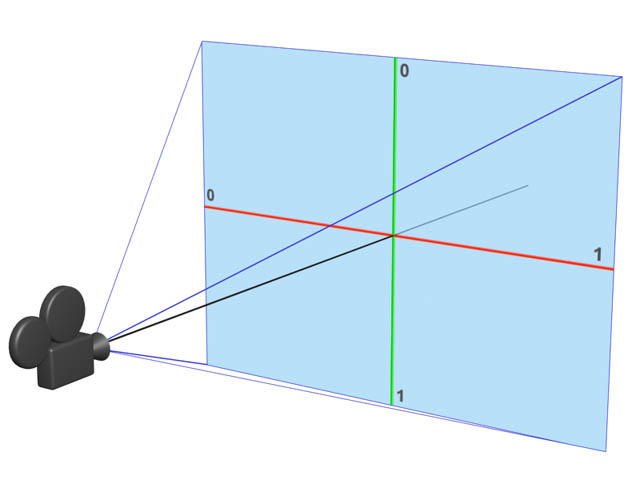
\includegraphics[width=9cm]{pics/camera01}
\end{center}
\end{methoddesc}

\begin{methoddesc}{getNearFar}{}
Return a 2-tuple (\var{near}, \var{far}) with the distances to the
near and far clipping planes. If automatic computation is disabled,
the method just returns the stored values, otherwise the values
are computed from the bounding box of the scene (which is converted
to a bounding sphere and the clipping planes are set as tangent planes
to the sphere).
\end{methoddesc}

% GLPointLight

\section{\class{GLPointLight} ---
         OpenGL point light}

\begin{classdesc}{GLPointLight}{name = ''GLPointLight'',\\ 
                       intensity = 1.0,\\
                       ambient = None,\\
                       diffuse = None,\\
                       specular = None,\\
                       constant_attenuation = 1.0,\\
                       linear_attenuation = 0.0,\\
                       quadratic_attenuation = 0.0,\\
                       enabled = True,\\
                       cast_shadow = False,\\
                       transform = None,\\
                       pos = None,\\
                       rot = None,\\
                       scale = None,\\
                       pivot = None,\\
                       offsetTransform = None,\\
                       auto_insert = True}

\end{classdesc}



% GLTargetSpotLight

\section{\class{GLTargetSpotLight} ---
         OpenGL target spot light}

\begin{classdesc}{GLTargetSpotLight}{name = ''GLTargetSpotLight'',\\ 
                       intensity = 1.0,\\
                       ambient = None,\\
                       diffuse = None,\\
                       specular = None,\\
                       constant_attenuation = 1.0,\\
                       linear_attenuation = 0.0,\\
                       quadratic_attenuation = 0.0,\\
                       exponent = 0.0,\\
                       cutoff = 45.0,\\
                       target = (0,0,0),\\
                       enabled = True,\\
                       cast_shadow = False,\\
                       transform = None,\\
                       pos = None,\\
                       rot = None,\\
                       scale = None,\\
                       pivot = None,\\
                       offsetTransform = None,\\
                       auto_insert = True}

\end{classdesc}



% GLFreeSpotLight

\section{\class{GLFreeSpotLight} ---
         OpenGL spot light}

\begin{classdesc}{GLFreeSpotLight}{name = ''GLFreeSpotLight'',\\ 
                       intensity = 1.0,\\
                       ambient = None,\\
                       diffuse = None,\\
                       specular = None,\\
                       constant_attenuation = 1.0,\\
                       linear_attenuation = 0.0,\\
                       quadratic_attenuation = 0.0,\\
                       exponent = 0.0,\\
                       cutoff = 45.0,\\
                       enabled = True,\\
                       cast_shadow = False,\\
                       transform = None,\\
                       pos = None,\\
                       rot = None,\\
                       scale = None,\\
                       pivot = None,\\
                       offsetTransform = None,\\
                       auto_insert = True}

\end{classdesc}



% GLTargetDistantLight

\section{\class{GLTargetDistantLight} ---
         OpenGL target distant light}

\begin{classdesc}{GLTargetDistantLight}{name = ''GLTargetDistantLight'',\\ 
                       intensity = 1.0,\\
                       ambient = None,\\
                       diffuse = None,\\
                       specular = None,\\
                       target = (0,0,0),\\
                       enabled = True,\\
                       cast_shadow = False,\\
                       transform = None,\\
                       pos = None,\\
                       rot = None,\\
                       scale = None,\\
                       pivot = None,\\
                       offsetTransform = None,\\
                       auto_insert = True}

\end{classdesc}



% GLFreeDistantLight

\section{\class{GLFreeDistantLight} ---
         OpenGL distant light}

\begin{classdesc}{GLFreeDistantLight}{name = ''GLFreeDistantLight'',\\ 
                       intensity = 1.0,\\
                       ambient = None,\\
                       diffuse = None,\\
                       specular = None,\\
                       enabled = True,\\
                       cast_shadow = False,\\
                       transform = None,\\
                       pos = None,\\
                       rot = None,\\
                       scale = None,\\
                       pivot = None,\\
                       offsetTransform = None,\\
                       auto_insert = True}

\end{classdesc}



% SpotLight3DS

\section{\class{SpotLight3DS} ---
         3DS spot light}

The \class{SpotLight3DS} class stores all parameters of the spot lights
as they are stored in 3DS files. The main purpose of this class is to
ensure that data doesn't get lost during file conversions.

This light sources can also be used for RenderMan renderings. However,
not all of the parameters are currently taken into account in the
corresponding RenderMan shader (see below).

\begin{classdesc}{SpotLight3DS}{name = "SpotLight3DS",\\ 
                       enabled = True,\\
                       intensity = 1.0,\\
                       color = (1,1,1),\\
                       see_cone = False,\\
                       roll = 0.0,\\
                       outer_range = 0,\\
                       inner_range = 0,\\
                       attenuation = 0,\\
                       rectangular_spot = 0,\\
                       shadowed = False,\\
                       shadow_bias = 0,\\
                       shadow_filter = 4.0,\\
                       shadow_size = 256,\\
                       spot_aspect = 0,\\
                       use_projector = False,\\
                       projector = 0,\\
                       overshoot = False,\\
                       ray_shadows = False,\\
                       ray_bias = False,\\
                       hotspot = 43,\\
                       falloff = 45,\\
	               target = (0,0,0)
                  }

\var{enabled} is a boolean flag that can be used to turn the light source
on or off.

\var{intensity} is the overall intensity of the light source. The higher
the value, the brighter the light.

\var{color} defines the color of the light source. It must be a sequence
of 3 floats containing RGB values.

\var{see_cone} ...

\var{roll} ...

\var{inner_range} and \var{outer_range} specify an intensity range based
on distance. Any parts of the scene that are nearer to the light source
than \var{inner_range} are fully illuminated. Within the range between
\var{inner_range} and \var{outer_range} the brightness drops off to 0
and objects further than \var{outer_range} are not illuminated at all.
These range values are only taken into account when \var{attenuation}
is not 0.

\var{rectangular_spot} ...

If \var{shadowed} is set to \code{True} the light casts a shadow.

\var{shadow_bias} is a small value greater than 0 that is used to prevent
invalid self-shadowing (i.e. so that a surface element doesn't shadow itself).

\var{shadow_filter} specifies the size of the filter when doing shadow map
lookups. The higher the value the blurrier the shadow.

\var{shadow_size} defines the size of the shadow map. The shadow map will
always be square and have a width of \var{shadow_size} pixels.

\var{spot_aspect} ...

\var{use_projector} ...

\var{projector} ...

If \var{overshoot} is \code{True} the light virtually becomes a point light
source, i.e. it also illuminates the parts of the scene that lie outside
its cone but the shadow is still restricted to the cone.

\var{ray_shadows} ...

\var{ray_bias} ...

\var{hotspot} This is the angle (in degrees) of the "inner" cone which is fully illuminated.

\var{falloff} This is the angle (in degrees) of the "outer" cone. The light 
intensity between the inner and outer cone drops off to 0. The region outside
the outer cone is not illuminated (unless \var{overshoot} is activated).

\var{target} is the target point that the light source aims at.

\end{classdesc}

The following parameters are used in the corresponding RenderMan
shader, all other parameters are currently ignored:

\begin{itemize}
\item intensity
\item color
\item falloff
\item hotspot
\item attenuation
\item inner_range
\item outer_range
\item overshoot
\item shadow_bias
\item shadow_filter
\item shadow_size
\end{itemize}

% SpotLight3DS

\section{\class{RMLightSource} ---
         RenderMan light source}

\begin{classdesc}{RMLightSource}{name = "RMLightSource",\\ 
                       shader = None
                  }


\var{shader} specifies the light shader that should be used. It
can either be a string containing the shader name or a \class{RMShader}
instance representing the shader (see section \ref{rmshader}).

\end{classdesc}


The parameters of the shader is made available as attributes of the
light source object. The corresponding slots can be obtained by adding
the suffix \code{_slot} to the name.


% RIBArchive component

\section{\class{RIBArchive} ---
         Reference an external RIB archive}

The \class{RIBArchive} class represents geometry that is defined in
an external RIB file. When the scene is rendered using a RenderMan
renderer the RIB file will be included via a call to 
\cfunction{RiReadArchive()}. In an interactive viewer, a \class{RIBArchive}
object will be invisible.

\begin{classdesc}{RIBArchive}{name = "RIBArchive",\\ 
                              filename = None, \\
                              auto_insert = True}

\var{filename} is the name of the external RIB file.

\end{classdesc}



% ODE joints

\section{ODE joints ---
         Joint classes for the ODEDynamics component}

%----------------------------------------------------------------------
\subsection{\class{ODEBallJoint} --- Ball and socket joint}

\begin{classdesc}{ODEBallJoint}{name = "ODEBallJoint",\\ 
                             body1 = None, \\
                             body2 = None
                             }

\end{classdesc}

%----------------------------------------------------------------------
\subsection{\class{ODEHingeJoint} --- Hinge joint}

\begin{classdesc}{ODEHingeJoint}{name = "ODEHingeJoint",\\ 
                             body1 = None, \\
                             body2 = None
                             }

\end{classdesc}

%----------------------------------------------------------------------
\subsection{\class{ODESliderJoint} --- Slider joint}

\begin{classdesc}{ODESliderJoint}{name = "ODESliderJoint",\\ 
                             body1 = None, \\
                             body2 = None
                             }

\end{classdesc}

%----------------------------------------------------------------------
\subsection{\class{ODEHinge2Joint} --- Hinge-2 joint}

\begin{classdesc}{ODEHinge2Joint}{name = "ODEHinge2Joint",\\ 
                             body1 = None, \\
                             body2 = None
                             }

\end{classdesc}

%----------------------------------------------------------------------
\subsection{\class{ODEUniversalJoint} --- Universal joint}

\begin{classdesc}{ODEUniversalJoint}{name = "ODEUniversalJoint",\\ 
                             body1 = None, \\
                             body2 = None
                             }

\end{classdesc}




% BezierCurve

\section{\class{BezierCurve} ---
         Bezier curve}

\begin{classdesc}{BezierCurve}{name = "BezierCurve",\\ 
                               pnts = None,\\
                               closed = False,\\
                               epsilon = 0.01,\\
                               subdiv = 4,\\
                               show_tangents = False,\\
                               curvegeom = None\\
                              }

\var{pnts} is a list of \class{BezierPoint} objects (see section
\ref{beziercurvegeom}).

If \var{closed} is set to \code{True} the last point will be connected
to the first point.

\var{epsilon} is a threshold value that determines the accuracy of
length calculations of the curve.

\var{subdiv} is the number of subdivisions that are made to draw the
curve using OpenGL.

If \var{show_tangents} is set to \code{True} the OpenGL visualization
will also show the in and out tangents.

You can also pass a previously created \class{BezierCurveGeom} object
via the \var{curvegeom} argument. In this case, the arguments \var{pnts},
\var{closed}, \var{epsilon}, \var{subdiv} and \var{show_tangents} are 
ignored.
\end{classdesc}





%---
\chapter{GeomObjects \label{geomobjects}}

% GeomObject

\section{\class{GeomObject} ---
         Geometry base class}

The \class{GeomObject} class is the base class for all geometries.
Instances of this class are stored in the \member{geom} attribute
of the world objects and can be shared among them.

\begin{classdesc}{GeomObject}{}
...params?...
\end{classdesc}

% Methods
\begin{methoddesc}{boundingBox}{}
Return the local axis aligned bounding box. The bounding box is
given with respect to the local transformation L (which is not
what you get from the transform slot of the world object).
\end{methoddesc}

\begin{methoddesc}{drawGL}{}
Draw the geometry using OpenGL commands.
\end{methoddesc}

\begin{methoddesc}{uniformCount}{}
Return the multiplicity of \keyword{UNIFORM} variables.
\end{methoddesc}

\begin{methoddesc}{varyingCount}{}
Return the multiplicity of \keyword{VARYING} variables.
\end{methoddesc}

\begin{methoddesc}{vertexCount}{}
Return the multiplicity of \keyword{VERTEX} variables.
\end{methoddesc}

\begin{methoddesc}{faceVaryingCount}{}
Return the multiplicity of \keyword{FACEVARYING} variables.
\end{methoddesc}

\begin{methoddesc}{faceVertexCount}{}
Return the multiplicity of \keyword{FACEVERTEX} variables.
\end{methoddesc}

\begin{methoddesc}{slotSizeConstraint}{storage}
Return a constraint object for primitive variable slots or None if the size
of the slot should be unconstrained.
This method is called when a new primitive variable is created. The
returned constraint object is used for the array slot that holds the
values of the variable. \var{storage} is the storage class of the new
variable which will be one of \code{UNIFORM}, \code{VARYING}, \code{VERTEX},
\code{FACEVARYING} or \code{FACEVERTEX}. The method will never be called
when \code{CONSTANT} or \code{USER} variables are created.
\end{methoddesc}

\begin{methoddesc}{newVariable}{name, storage, type, multiplicity=1, user_n=0}
Attaches a new primitive variable to the geometry.

\var{storage} specifies the storage
class, i.e. how many values are actually stored. It must be one of
\code{CONSTANT}, \code{UNIFORM}, \code{VARYING}, \code{VERTEX}, 
\code{FACEVARYING}, \code{FACEVERTEX} or
\code{USER}. The exact number of values depends on the actual geometry.
However, \code{CONSTANT} is always exactly one value for the entire
geometry and \code{USER} is a user defined number specified in \var{user_n}.

\var{type} is the type of the variable and must be one of 
\code{INT}, \code{FLOAT}, \code{STRING}, \code{COLOR}, \code{POINT}, 
\code{VECTOR}, \code{NORMAL}, \code{MATRIX} and \code{HPOINT}. 
If \var{multiplicity} is greater than 1, then an array with that size is
created. 

Creating a new variable will always create a new slot of that name as well.
The slot is always an \class{ArraySlot} (even for \code{CONSTANT} variables).
After you have created a variable you can use the corresponding slot to
manipulate the values of the variable.

Here is an example of a "varying int [3]" variable that's created on a sphere 
geometry. This means, the variable will consist of four 3-tuples of integers
(one for each parametric corner).

\begin{verbatim}
>>> from cgkit.all import *
>>> sg=SphereGeom()
>>> sg.newVariable("foo", VARYING, INT, multiplicity=3)
>>> for v in sg.iterVariables(): print v
...
('foo', cgkit._core.VarStorage.VARYING, cgkit._core.VarType.INT, 3)
>>> s=sg.slot("foo")
>>> s[1]=(1,2,3)
>>> for f in s: print f
...
(0, 0, 0)
(1, 2, 3)
(0, 0, 0)
(0, 0, 0)
\end{verbatim}
\end{methoddesc}

\begin{methoddesc}{deleteVariable}{name}
Delete the primitive variable with the specified name.
\end{methoddesc}

\begin{methoddesc}{deleteAllVariables}{}
Delete all primitive variables.
\end{methoddesc}

\begin{methoddesc}{findVariable}{name}
Search for a particular primitive variable and return its descriptor.
\code{None} is returned if a variable called \var{name} cannot be found.
The return value is a 4-tuple (name, storage class, type, multiplicity)
describing the variable. See the \method{newVariable()} method for a
description of the individual elements.
\end{methoddesc}

\begin{methoddesc}{iterVariables}{}
Return an iterator that iterates over all existing primitive variables.
The iterator will return the same 4-tuple as returned by 
\method{findVariable()}.
\end{methoddesc}

\begin{methoddesc}{convert}{targetgeom}
Convert the geometry into another type of geometry. \var{targetgeom}
is another \class{GeomObject} that will receive the result of the
conversion.  If the conversion is not possible, a
\exception{NotImplementedError} exception is thrown.

In the following example, a box geometry is converted into a triangle
mesh:

\begin{verbatim}
>>> bg=BoxGeom(segmentsx=3, segmentsy=3, segmentsz=3)
>>> tm=TriMeshGeom()
>>> bg.convert(tm)
>>> print len(tm.verts)
56
>>> print len(tm.faces)
108
\end{verbatim}
\end{methoddesc}




% BoxGeom

\section{\class{BoxGeom} ---
         Box geometry}

\begin{classdesc}{BoxGeom}{lx=1.0, ly=1.0, lz=1.0, segmentsx=1, segmentsy=1, segmentsz=1}

\var{lx}, \var{ly} and \var{lz} specify the dimensions of the box in
the respective direction.

\var{segmentsx}, \var{segmentsy} and \var{segmentsz} are the number of
segments in each direction.
\end{classdesc}

A \class{BoxGeom} has the following slots:

\begin{tableiv}{l|l|c|l}{code}{Slot}{Type}{Access}{Description}
\lineiv{cog_slot}{vec3}{r}{The local center of gravity}
\lineiv{inertiatensor_slot}{mat3}{r}{The local inertia tensor}
\lineiv{lx_slot}{float}{rw}{The length in x direction}
\lineiv{ly_slot}{float}{rw}{The length in y direction}
\lineiv{lz_slot}{float}{rw}{The length in z direction}
\lineiv{segmentsx_slot}{int}{rw}{The number of segments in x direction}
\lineiv{segmentsy_slot}{int}{rw}{The number of segments in y direction}
\lineiv{segmentsz_slot}{int}{rw}{The number of segments in z direction}
\end{tableiv}

% Attributes
\begin{memberdesc}{cog}
Center of gravity with respect to the local coordinate system.
\end{memberdesc}

\begin{memberdesc}{inertiatensor}
Inertia tensor with respect to the local coordinate system.
\end{memberdesc}

\begin{memberdesc}{lx}
The length in x direction.
\end{memberdesc}

\begin{memberdesc}{ly}
The length in y direction.
\end{memberdesc}

\begin{memberdesc}{lz}
The length in z direction.
\end{memberdesc}

\begin{memberdesc}{segmentsx}
The number of segments in x direction.
\end{memberdesc}

\begin{memberdesc}{segmentsy}
The number of segments in y direction.
\end{memberdesc}

\begin{memberdesc}{segmentsz}
The number of segments in z direction.
\end{memberdesc}








% SphereGeom

\section{\class{SphereGeom} ---
         Sphere geometry}

\begin{classdesc}{SphereGeom}{radius=1.0, segmentsu=16, segmentsv=8}
\var{radius} is the radius in the local coordinate system.

\var{segmentsu} and \var{segmentsv} are used when the sphere has to
be tesselated (either for interactive display or when converted to
a triangle mesh).
\end{classdesc}

A \class{SphereGeom} has the following slots:

\begin{tableiv}{l|l|c|l}{code}{Slot}{Type}{Access}{Description}
\lineiv{cog_slot}{vec3}{r}{The local center of gravity}
\lineiv{inertiatensor_slot}{mat3}{r}{The local inertia tensor}
\lineiv{radius_slot}{float}{rw}{The radius}
\lineiv{segmentsu_slot}{int}{rw}{The number of segments in u direction}
\lineiv{segmentsv_slot}{int}{rw}{The number of segments in v direction}
\end{tableiv}

% Attributes
\begin{memberdesc}{cog}
Center of gravity with respect to the local coordinate system.
\end{memberdesc}

\begin{memberdesc}{inertiatensor}
Inertia tensor with respect to the local coordinate system.
\end{memberdesc}

\begin{memberdesc}{radius}
The radius of the sphere.
\end{memberdesc}

\begin{memberdesc}{segmentsu}
The number of segments in u direction.
\end{memberdesc}

\begin{memberdesc}{segmentsv}
The number of segments in v direction.
\end{memberdesc}







% CCylinderGeom

\section{\class{CCylinderGeom} ---
         Capped cylinder geometry}

\begin{classdesc}{CCylinderGeom}{radius=1.0, length=1.0, segmentsu=16, segmentsvl=1, segmentsvr=4}

\var{radius} is the radius of the cylinder and caps in the local coordinate 
system.

\var{length} is the length of the cylinder (not counting the caps).

\var{segmentsu} is the number of segments in u direction, \var{segmentsvl}
the number of segments of the cylinder part and \var{segmentsvr} the
number of segments for each cap.
\end{classdesc}

A \class{CCylinderGeom} has the following slots:

\begin{tableiv}{l|l|c|l}{code}{Slot}{Type}{Access}{Description}
\lineiv{cog_slot}{vec3}{r}{The local center of gravity}
\lineiv{inertiatensor_slot}{mat3}{r}{The local inertia tensor}
\lineiv{radius_slot}{float}{rw}{The radius of the cylinder}
\lineiv{length_slot}{float}{rw}{The lenght of the cylinder}
\lineiv{segmentsu_slot}{int}{rw}{The number of segments in u direction}
\lineiv{segmentsvl_slot}{int}{rw}{The number of cylinder segments in v direction}
\lineiv{segmentsvr_slot}{int}{rw}{The number of cap segments in v direction}
\end{tableiv}

% Attributes
\begin{memberdesc}{cog}
Center of gravity with respect to the local coordinate system.
\end{memberdesc}

\begin{memberdesc}{inertiatensor}
Inertia tensor with respect to the local coordinate system.
\end{memberdesc}

\begin{memberdesc}{radius}
The radius of the cylinder and caps.
\end{memberdesc}

\begin{memberdesc}{length}
The length of the cylinder (not counting the caps).
\end{memberdesc}

\begin{memberdesc}{segmentsu}
The number of segments in u direction.
\end{memberdesc}

\begin{memberdesc}{segmentsvl}
The number of cylinder segments in v direction.
\end{memberdesc}

\begin{memberdesc}{segmentsvr}
The number of cap segments in v direction.
\end{memberdesc}

% PlaneGeom

\section{\class{PlaneGeom} ---
         Plane geometry}

\begin{classdesc}{PlaneGeom}{lx=1.0, ly=1.0, segmentsx=1, segmentsy=1}

\var{lx} and \var{ly} specify the dimensions of the plane in
the respective direction.

\var{segmentsx} and \var{segmentsy} are the number of
segments in each direction.
\end{classdesc}

A \class{PlaneGeom} has the following slots:

\begin{tableiv}{l|l|c|l}{code}{Slot}{Type}{Access}{Description}
\lineiv{lx_slot}{float}{rw}{The length in x direction}
\lineiv{ly_slot}{float}{rw}{The length in y direction}
\lineiv{segmentsx_slot}{int}{rw}{The number of segments in x direction}
\lineiv{segmentsy_slot}{int}{rw}{The number of segments in y direction}
\end{tableiv}

% Attributes
\begin{memberdesc}{lx}
The length in x direction.
\end{memberdesc}

\begin{memberdesc}{ly}
The length in y direction.
\end{memberdesc}

\begin{memberdesc}{segmentsx}
The number of segments in x direction.
\end{memberdesc}

\begin{memberdesc}{segmentsy}
The number of segments in y direction.
\end{memberdesc}







% TorusGeom

\section{\class{TorusGeom} ---
         Torus geometry}

\begin{classdesc}{TorusGeom}{major=1.0, minor=0.1, segmentsu=16, segmentsv=8}
\end{classdesc}








% TriMeshGeom

\section{\class{TriMeshGeom} ---
         Triangle mesh geometry}

\begin{classdesc}{TriMeshGeom}{}
Creates an empty triangle mesh.
\end{classdesc}

A \class{TriMeshGeom} has the following slots:

\begin{tableiv}{l|l|c|l}{code}{Slot}{Type}{Access}{Description}
\lineiv{cog_slot}{vec3}{r}{The local center of gravity}
\lineiv{inertiatensor_slot}{mat3}{r}{The local inertia tensor}
\lineiv{verts_slot}{vec3 array}{rw}{The mesh vertices}
\lineiv{faces_slot}{int[3] array}{rw}{The mesh faces}
\end{tableiv}

% Attributes
\begin{memberdesc}{cog}
Center of gravity with respect to the local coordinate system of the 
triangle mesh.
\end{memberdesc}

\begin{memberdesc}{inertiatensor}
Inertia tensor with respect to the local coordinate system of the 
triangle mesh.
\end{memberdesc}

\begin{memberdesc}{verts}
This attribute contains the sequence of mesh vertices.
\end{memberdesc}

\begin{memberdesc}{faces}
This attribute contains the sequence of mesh faces. Each face contains
three vertex indices.
\end{memberdesc}

% Methods
\begin{methoddesc}{intersectRay}{origin, direction, earlyexit=False}
Intersect a ray with the mesh. The ray starts at \var{origin} and
travels along \var{direction} which must both be of type \class{vec3}.
\var{origin} and \var{direction} must be given with respect to the
local coordinate system L of the geometry. If \var{earlyexit} is
\code{True} the method returns after the first hit, otherwise all
triangles are tested and the result contains the nearest hit.
The return value is a tuple (\var{hit}, \var{t}, \var{faceindex}, 
\var{u}, \var{v}) where \var{hit} is a boolean that indicates if
the mesh was hit or not. \var{t} is the ray parameter, i.e. the
point of intersection is at \var{origin} + t*\var{direction}.
\var{faceindex} is the index of the face that was hit and \var{u}
\var{v} are the parameter coordinates of the intersection point.

This method tests the ray with all triangles, so it is not efficient if
you have a lot of rays to test. It is meant for only a few rays where
the preprocessing cost wouldn't be amortized.
 
The ray-triangle intersection code (non-culling case) is based on:
 
Tomas M�ller and Ben Trumbore\\
{\em Fast, minimum storage ray-triangle intersection}\\
Journal of graphics tools, 2(1):21-28, 1997\\
\url{http://www.acm.org/jgt/papers/MollerTrumbore97/}
\end{methoddesc}






% PolyhedronGeom

\section{\class{PolyhedronGeom} ---
         Polyhedron geometry}

The \class{PolyhedronGeom} class stores a collection of general planar
concave polygons that may also contain holes. Each polygon is described
by a sequence of vertex loops. The first loop defines the polygon boundary
and each subsequent loop describes a hole. Each loop is a sequence of
vertex indices.

\begin{classdesc}{PolyhedronGeom}{}
Creates an empty polyhedron.
\end{classdesc}

A \class{PolyhedronGeom} has the following slots:

\begin{tableiv}{l|l|c|l}{code}{Slot}{Type}{Access}{Description}
\lineiv{verts_slot}{vec3 array}{rw}{The polygon vertices}
\end{tableiv}

% Attributes
\begin{memberdesc}{verts}
This attribute contains the sequence of polygon vertices.
\end{memberdesc}

% Methods
\begin{methoddesc}{hasPolysWithHoles}{}
Return \code{True} if there is at least one polygon with a hole.
\end{methoddesc}

\begin{methoddesc}{getNumPolys}{}
Return the number of polygons.
\end{methoddesc}

\begin{methoddesc}{getNumLoops}{poly}
Return the number of vertex loops in the polygon with index \var{poly}.
\end{methoddesc}

\begin{methoddesc}{getNumVerts}{poly, loop}
Return the number of vertex indices in one particular loop. \var{poly}
is the polygon index and \var{loop} the loop index.
\end{methoddesc}

\begin{methoddesc}{setNumPolys}{num}
Allocate space for \var{num} polygons.
\end{methoddesc}

\begin{methoddesc}{setNumLoops}{poly, num}
Allocate space for \var{num} loops in the polygon with index \var{poly}.
\end{methoddesc}

\begin{methoddesc}{getLoop}{poly, loop}
Return a loop from a polygon. \var{poly} is the polygon index and \var{loop}
the loop index. The return value is a sequence of vertex indices.
\end{methoddesc}

\begin{methoddesc}{setLoop}{poly, loop, vloop}
Set a new polygon loop. \var{poly} is the polygon index, \var{loop}
the loop index and \var{vloop} a sequence of vertex indices.
\end{methoddesc}

\begin{methoddesc}{getPoly}{poly}
Return a polygon. \var{poly} is the polygon index. The return value
is a sequence of vertex loops.
\end{methoddesc}

\begin{methoddesc}{setPoly}{poly, polydef}
Set a polygon. \var{poly} is the polygon index and \var{polydef} a sequence
of vertex loops.
\end{methoddesc}





% BezierCurveGeom

\section{\class{BezierCurveGeom} ---
         Piecewise cubic Bezier curve}
\label{beziercurvegeom}

The \class{BezierCurveGeom} class represents a piecewise cubic curve
in 3D space that is composed of an arbitrary number of cubic Bezier
segments. The class stores a number of 3D points that are interpolated
by the curve. Each point has an in tangent and an out tangent associated
with it that define how the curve enters and leaves the point.

\begin{classdesc}{BezierPoint}{pos, intangent=vec3(0), outtangent=vec3(0)}

This class just stores a position and the in and out tangents and
is used to pass these parameters to the constructor of a 
\class{BezierCurveGeom}.

\var{pos} is a point position that the curve will interpolate.

\var{intangent} and \var{outtangent} define where the curve enters
and leaves the point.
\end{classdesc}


\begin{classdesc}{BezierCurveGeom}{pnts = None,\\
                                   closed = False,\\
                                   epsilon = 0.01,\\
                                   subdiv = 4,\\
                                   show_tangents = False}

\var{pnts} is a list of \class{BezierPoint} objects describing the
points to interpolate and the in and out tangents.

If \var{closed} is set to \code{True} the last point will be connected
to the first point.

\var{epsilon} is a threshold value that determines the accuracy of
length calculations of the curve.

\var{subdiv} is the number of subdivisions that are made to draw the
curve using OpenGL.

If \var{show_tangents} is set to \code{True} the OpenGL visualization
will also show the in and out tangents.
\end{classdesc}

A \class{BezierCurveGeom} has the following slots:

\begin{tableiv}{l|l|c|l}{code}{Slot}{Type}{Access}{Description}
\lineiv{pnts_slot}{[vec3]}{rw}{The curve points}
\lineiv{intangents_slot}{[vec3]}{rw}{The in tangents}
\lineiv{outtangents_slot}{[vec3]}{rw}{The out tangents}
\end{tableiv}

\begin{memberdesc}{closed}
This is a boolean indicating wheter the curve is closed or not. You
can read and write this attribute.
\end{memberdesc}

\begin{memberdesc}{numsegs}
The number of Bezier segments in the curve. You can only read this
attribute.
\end{memberdesc}

\begin{memberdesc}{paraminterval}
This is a tuple (\var{t_min}, \var{t_max}) containing the valid parameter
interval of the curve. You can only read this attribute.
\end{memberdesc}

% eval
\begin{methoddesc}{eval}{t}
Evaluate the curve at parameter \var{t} and return the curve point.
\end{methoddesc}

% evalFrame
\begin{methoddesc}{evalFrame}{t}
Evaluate the curve at parameter \var{t} and return the curve point,
the tangent and the second derivative.
\end{methoddesc}

% deriv
\begin{methoddesc}{deriv}{t}
Return the first derivative (the tangent) at parameter \var{t}.
\end{methoddesc}

% arcLen
\begin{methoddesc}{arcLen}{t}
Return the arc length of the curve up to the point specified by the parameter
\var{t}.
\end{methoddesc}

% length
\begin{methoddesc}{length}{}
Return the entire length of the curve. This is equivalent to 
\code{arcLen(t_max)}.
\end{methoddesc}








%---
\chapter{Materials \label{materials}}

% GLMaterial

\section{\class{GLMaterial} ---
         OpenGL material}

The \class{GLMaterial} class represents the material model of the standard
OpenGL API. All colors are represented as (r,g,b,a). If you don't use
blending you can leave out the alpha value in the constructor.

\begin{classdesc}{GLMaterial}{name = "GLMaterial",\\ 
                              ambient = (0.2, 0.2, 0.2, 1.0),\\
                              diffuse = (0.7, 0.7, 0.7, 1.0),\\
                              specular = (0, 0, 0, 1),\\
                              shininess = 0.0,\\
                              emission = (0, 0, 0, 1),\\
                              blend_factors = None,\\
                              texture = None,\\
                              vertex_shader = None,\\
                              fragment_shader = None,\\
                              density = 1.0}

\var{ambient} is the ambient color of the material.

\var{diffuse} is the diffuse color of the material.

\var{specular} is the color of the specular highlight.

\var{shininess} determines the size of the highlight and lies 
between 0.0 and 128.0. The higher the value, the smaller and brighter
the highlight.

The \var{emission} color can be used to simulate objects that emit light.

\var{blend_factors} is a 2-tuple with the parameters for the 
\cfunction{glBlendFunc()} call which indicate how to compute the
source and destination blend factors 
(see \ulink{\cfunction{glBlendFunc()}}{http://pyopengl.sourceforge.net/documentation/manual/glBlendFunc.3G.html}).
Blending is disabled if \var{blend_factors} is \code{None}.

\var{texture} is either \code{None}, a single \class{GLTexture} object or
a list of \class{GLTexture} objects specifying the texture image(s) to use.

\var{vertex_shader} is either \code{None}, a single \class{GLShader} object
or a list of \class{GLShader} objects specifying the vertex shaders to use.

\var{fragment_shader} is either \code{None}, a single \class{GLShader} object
or a list of \class{GLShader} objects specifying the fragment shaders to use.

\var{density} is the density value used for physical simulations.
\end{classdesc}

% Methods
\begin{methoddesc}{getNumTextures}{}
Return the current size of the texture array.
\end{methoddesc}

\begin{methoddesc}{setNumTextures}{num}
Set a new size for the texture array.
\end{methoddesc}

\begin{methoddesc}{getTexture}{idx=0}
Get a stored texture. The method returns \code{None} if the given index
is out of range or if there is no texture stored at that position.
\end{methoddesc}

\begin{methoddesc}{setTexture}{tex, idx=0}
Set a new texture. An \exception{IndexError} exception is thrown if the 
index is out of range.
\end{methoddesc}

\begin{methoddesc}{getNumVertexShaders}{}
Return the current size of the vertex shader array.
\end{methoddesc}

\begin{methoddesc}{setNumVertexShaders}{num}
Set a new size for the vertex shader array.
\end{methoddesc}

\begin{methoddesc}{getVertexShader}{idx=0}
Get a vertex shader object. The method returns \code{None} if the given index
is out of range or if there is no shader object stored at that position.
\end{methoddesc}

\begin{methoddesc}{setVertexShader}{shader, idx=0}
Set a new vertex shader object. An \exception{IndexError} exception is 
thrown if the index is out of range. A ValueError exception is thrown if the 
shader is not of type \code{VERTEX}.
\end{methoddesc}

\begin{methoddesc}{getNumFragmentShaders}{}
Return the current size of the fragment shader array.
\end{methoddesc}

\begin{methoddesc}{setNumFragmentShaders}{num}
Set a new size for the fragment shader array.
\end{methoddesc}

\begin{methoddesc}{getFragmentShader}{idx=0}
Get a fragment shader object. The method returns \code{None} if the given index
is out of range or if there is no shader object stored at that position.
\end{methoddesc}

\begin{methoddesc}{setFragmentShader}{shader, idx=0}
Set a new fragment shader object. An \exception{IndexError} exception is 
thrown if the index is out of range. A ValueError exception is thrown if the 
shader is not of type \code{FRAGMENT}.
\end{methoddesc}

%-----------------------
\subsection{\class{GLTexture} --- Specifying a texture map}

The \class{GLTexture} class is used to describe the parameters of an
OpenGL texture map for use with the \class{GLMaterial} class.

\begin{classdesc}{GLTexture}{imagename = "",\\
                             image = None,\\ 
                             mode = GL_DECAL,\\
                             mipmap = True,\\
                             mag_filter = GL_LINEAR,\\
                             min_filter = GL_LINEAR,\\
                             wrap_s = GL_REPEAT,\\
                             wrap_t = GL_REPEAT,\\
                             internalformat = GL_RGB,\\
                             texenvcolor = vec4(1),\\
                             transform = mat4(1),\\
                             size = None, \\
                             environment_map = False\\
                            }

\var{imagename} is the name of the image file that should be used as a
texture map. If the image resolution is not a power of 2, the image
is scaled up to the next higher power of 2 resolution.

It is also possible to pass the actual image data in the \var{image}
parameter.  The image can either be a PIL image or the raw RGB
data. In the latter case, you must explicitly specify the image
resolution (which must then be a power of 2 resolution) in the \var{size}
argument. The \var{imagename} argument is ignored if the data is passed
via the \var{image} argument.

\var{mode} specifies how the image is applied to the object. It can be
one of \code{GL_REPLACE}, \code{GL_MODULATE}, \code{GL_DECAL} and 
\code{GL_BLEND}. In the latter
case, the blend color is given by \var{texenvcolor} 
(see \ulink{\cfunction{glTexEnv()}}{http://pyopengl.sourceforge.net/documentation/manual/glTexEnv.3G.html}).

\var{mipmap} determines whether mip mapping should be used or not.

\var{mag_filter} is the filter to use when magnification occurs (i.e. when
the texture appears larger on screen that it actually is). It can be
either \code{GL_NEAREST} or \code{GL_LINEAR}.

\var{min_filter} is the filter to use when minification occurs (i.e. when
the texture appears smaller on screen that it actually is). It can be one
of following values
(see \ulink{\cfunction{glTexParameter()}}{http://pyopengl.sourceforge.net/documentation/manual/glTexParameter.3G.html}):
%\code{GL_NEAREST}, \code{GL_LINEAR}, \code{GL_NEAREST_MIPMAP_NEAREST},
%\code{GL_NEAREST_MIPMAP_LINEAR}, \code{GL_LINEAR_MIPMAP_NEAREST} or
%\code{GL_LINEAR_MIPMAP_LINEAR}

\begin{itemize}
\item \code{GL_NEAREST}
\item \code{GL_LINEAR}
\item \code{GL_NEAREST_MIPMAP_NEAREST}
\item \code{GL_NEAREST_MIPMAP_LINEAR}
\item \code{GL_LINEAR_MIPMAP_NEAREST}
\item \code{GL_LINEAR_MIPMAP_LINEAR}
\end{itemize}

If \code{GL_LINEAR} is specified and mip mapping
is used then the filter is automatically set to \code{GL_LINEAR_MIPMAP_LINEAR}

\var{wrap_s} and \var{wrap_t} specify what happens if the texture coordinate
leave the range 0-1. They can be one of \code{GL_REPEAT}, \code{GL_CLAMP}
and \code{GL_CLAMP_TO_EDGE}
(see \ulink{\cfunction{glTexParameter()}}{http://pyopengl.sourceforge.net/documentation/manual/glTexParameter.3G.html}).

\var{internalformat} specifies how the image data will be stored in memory.
Usually, you'll either specify \code{GL_RGB} or \code{GL_RGBA} if you have
alpha values in your image and you want to use them
(see \ulink{\cfunction{glTexImage2D()}}{http://pyopengl.sourceforge.net/documentation/manual/glTexImage2D.3G.html}).

\var{transform} is a transformation that is applied to the texture coordinates.

\var{size} is a 2-tuple containing the desired texture map resolution which
must be a power of 2. The image is resized to the specified resolution.
If \var{size} is \code{None} then the next higher power of 2 value is used.

If \var{environment_map} is \code{True} the image is used as a 
latitude/longitude environment map.

\end{classdesc}

%-----------------------
\subsection{\class{GLShader} --- Specifying a shader}

The \class{GLShader} class is used to add a OpenGL 2 shader source file
to a \class{GLMaterial} class.

\begin{classdesc}{GLShader}{shadertype,\\
                            filename,\\ 
                            cpp = None,\\
                            cpperrstream = sys.stderr,\\
                            **shaderparams
                            }

\var{shadertype} specifies whether this shader is vertex shader or a
fragment shader. The value can either be \code{GLShader.ShaderType.VERTEX}
(or \code{GLSLANG_VERTEX}) or \code{GLShader.ShaderType.FRAGMENT}
(or \code{GLSLANG_FRAGMENT}).

\var{filename} is the shader source file name.

\var{cpp} determines the preprocessor that should be used when extracting
shader parameters. \var{cpperrstream} is used to output errors from the
preprocessor (see the function \function{glslangparams.glslangparams()} 
(section \ref{glslangparams}) for details).

Any additional keyword argument is assumed to be a shader parameter.
\end{classdesc}


% RMMaterial

\section{\class{RMMaterial} ---
         RenderMan material}

The \class{RMMaterial} class is a special material that is only of
use if you are creating images via a RenderMan renderer and you want
to write your shaders in external shader files or use shaders that
are already compiled.

The material may consist of a surface shader, a displacement shader
and an interior shader. The shader source files (or only the shader
names) are passed via \class{RMShader} instances as arguments to the
constructor. If the \class{RMShader} instance points to a file, the
material object will take care of the compilation of the
file. Otherwise, it is up to you to compile the shader and make sure
that the renderer can find it.

\begin{classdesc}{RMMaterial}{name = "RMMaterial", \\
                              surface = None,\\
                              displacement = None,\\
                              displacementbound = ("current", 0.0),\\
                              interior = None,\\
                              color = None,\\
                              opacity = None
                             }


\var{surface} specifies the surface shader to use. It can either be
a string containing the shader name or a \class{RMShader} instance
representing the shader. You can also pass \code{None} if no surface
shader should be instantiated.

\var{displacment} specifies the displacment shader to use. It can either be
a string containing the shader name or a \class{RMShader} instance
representing the shader. You can also pass \code{None} if no displacment
shader should be instantiated.

\var{displacementbound} is a tuple (coordinate system, distance) that
specifies the maximum displacement. The distance is the maximum amount that
a surface point is displaced and  is given in the specified coordinate 
system.

\var{interior} specifies the interior shader to use. It can either be
a string containing the shader name or a \class{RMShader} instance
representing the shader. You can also pass \code{None} if no interior
shader should be instantiated.

\var{color} is the color that should be set via \cfunction{RiColor()}.

\var{opacity} is the opacity that should be set via \cfunction{RiOpacity()}.
\end{classdesc}

The parameters of the shaders are made available as attributes of the
material objects. The corresponding slots can be obtained by adding
the suffix \code{_slot} to the name. Attribute names in the surface shader
have priority over the attributes in the displacement shader which in
turn has priority over the interior shader. This means, if there are
identical parameter names in all shaders you will access the parameter
of the surface shader. You can also access the attributes of each
shader via the \var{surface}, \var{displacement} and \var{interior}
attributes which contain the corresponding \class{RMShader} instances.

Example:
   
\begin{verbatim}
mat = RMMaterial(surface = RMShader("mysurface.sl"),
                 displacement = RMShader("c:\\shaders\\dented.sl"),
                 color = (1,0.5,0.8)
                 )
...
Sphere(pos=(1,2,3), radius=0.5, material=mat)
\end{verbatim}

In this example, the material uses the surface shader \file{mysurface.sl}
and the displacement shader \file{c:\textbackslash shaders\textbackslash dented.sl}. The shaders will
be compiled automatically because the shader source files are given
(instead of just the shader names).

%------------------------------------------------------------
\subsection{\class{RMShader} ---  RenderMan shader}
\label{rmshader}

The \class{RMShader} class encapsulates a single RenderMan shader.

\begin{classdesc}{RMShader}{shader = None, \\
                            transform = mat4(1), \\
                            cpp = None, \\
                            cpperrstream = sys.stderr, \\
                            params = None, \\
                            paramlist}
	
\var{shader} is either the name of a shader or the shader source file.
If a shader file is given then the shader is read to extract the parameters.
Each parameter will be made available as slot.

\var{transform} is a \class{mat4} containing a transformation that should
be applied to the shader. This means you can transform the shader relative
to the object it is applied to.

\var{cpp} determines the preprocessor that should be used when extracting
parameters. \var{cpperrstream} is used to output errors from the
preprocessor (see the function \function{slparams.slparams()} (section
\ref{slparams}) for details).

\var{params} can be used to declare parameters if the shader source
is not available. The value must be a dictionary that contains
token/value pairs. The token may contain an inline declaration. 

Any additional keyword argument is also considered to be a shader
parameter. However, this parameter cannot have an inline declaration,
so it is recommended to declare the parameter afterwards using the
\method{declare()} method, otherwise no declaration will be 
written in the RIB file and you have to care about the declaration
yourself.
\end{classdesc}

% shaderName
\begin{methoddesc}{shaderName}{}
Return the shader name or \code{None} if the name is not known.
\end{methoddesc}

% shaderType
\begin{methoddesc}{shaderType}{}
Return the shader type as a string (\code{"surface"}, \code{"displacement"},
\code{"light"}, ...) or \code{None} if the type is not known.
\end{methoddesc}

% declare
\begin{methoddesc}{declare}{name, type=None, cls=None, arraysize=None, default=None}
Declare a shader parameter. \var{name} is the parameter
name. \var{name} may also contain the entire declaration in SL
syntax. In this case, all other arguments are ignored, otherwise they
provide the missing information. \var{type} is the only parameter that is
mandatory if name does not contain the entire declaration. It contains
the name of the SL parameter type (float, string, color, point, vector,
normal, matrix). \var{cls} is the storage class (uniform, varying).
\var{arraysize} specifies the size of the array and \var{default} contains
the default value.

When a parameter is declared it is added to the list of known
parameters and a corresponding slot (\code{<name>_slot}) is created.

Examples:

\begin{verbatim}
shader.declare('uniform float Ka=0.5')
shader.declare('uniform float Ka')
shader.declare('float Ka')
shader.declare('Ka', type='float')
\end{verbatim}

A parameter that was specified in the constructor is used as default value
when the parameter is declared. In this case, any default value passed to
the \function{declare()} method is ignored.
\end{methoddesc}

% params
\begin{methoddesc}{params}{}
Return a dictionary containing the parameters for the current time.
The key is the parameter name (containing an inline declaration if
available) and the value is the current value of the parameter.
\end{methoddesc}

% Material3DS

\section{\class{Material3DS} ---
         3DS material}

\begin{classdesc}{Material3DS}{name = "Material3DS",\\ 
                              ambient = (0,0,0,0),\\
                              diffuse = (1.0, 1.0, 1.0, 1.0),\\
                              specular = (1.0, 1.0, 1.0, 1.0),\\
                              shininess = 1.0,\\
                              shin_strength = 0,\\
                              use_blur = 0,\\
                              transparency = 0.0,\\
                              falloff = 0,\\
                              additive = 0,\\
                              use_falloff = 0,\\
                              self_illum = False,\\
                              self_ilpct = 0.0,\\
                              shading = 0,\\
                              soften = 0,\\
                              face_map = 0,\\
                              two_sided = 0,\\
                              map_decal = 0,\\
                              use_wire = 0,\\
                              use_wire_abs = 0,\\
                              wire_size = 0,\\
                              density = 0,\\
                              texture1_map = None,\\
                              texture1_mask = None,\\
                              texture2_map = None,\\
                              texture2_mask = None,\\
                              opacity_map = None,\\
                              opacity_mask = None,\\
                              bump_map = None,\\
                              bump_mask = None,\\
                              specular_map = None,\\
                              specular_mask = None,\\
                              shininess_map = None,\\
                              shininess_mask = None,\\
                              self_illum_map = None,\\
                              self_illum_mask = None,\\
                              reflection_map = None,\\
                              reflection_mask = None,\\
                              bump_size = 1.0
	                      }
\end{classdesc}


%-----------------------
\subsection{\class{TextureMap3DS} --- Texture map definition for the 3DS material}

\begin{classdesc}{TextureMap3DS}{name,\\
                                 flags = 0,\\
                                 percent = 0.0,\\
                                 blur = 0.0,\\
                                 scale = (1.0, 1.0),\\
                                 offset = (0.0, 0.0),\\
                                 rotation = 0.0,\\
                                 tint1 = (0,0,0),\\
                                 tint2 = (0,0,0),\\
                                 tintr = (0,0,0),\\
                                 tintg = (0,0,0),\\
                                 tintb = (0,0,0),\\
                                }
\end{classdesc}

% OBJMaterial

\section{\class{OBJMaterial} ---
         OBJ material}
\label{objmaterial}

The \class{OBJMaterial} class stores the parameters of materials
as specified in a MTL file (which is the material file that accompanies 
a Wavefront OBJ file).

\begin{classdesc}{OBJMaterial}{name = "OBJMaterial",\\ 
                               illum = 2,\\
                               Ka = (0.2, 0.2, 0.2),\\
                               Kd = (0.8, 0.8, 0.8),\\
                               Ks = (0.0, 0.0, 0.0),\\
                               Ke = (0.0, 0.0, 0.0),\\
                               Ns = 0.0,\\
                               Ni = 1.0,\\
                               d = 1.0,\\
                               Tr = 1.0,\\
                               Tf = (1.0, 1.0, 1.0),\\
                               sharpness = 0.0,\\
                               map_Ka = None,\\
                               map_Kd = None,\\
                               map_Ks = None,\\
                               map_Ke = None,\\
                               map_Ns = None,\\
                               map_d = None,\\
                               map_Bump = None,\\
                               density = 1.0\\
	                      }

\var{illum} sepcifies the illumination mode (0=constant, 1=diffuse, 2=diffuse+specular, ...).

\var{Ka} is the ambient color.

\var{Kd} is the diffuse color.

\var{Ks} is the specular color.

\var{Ke} is the emissive color.

\var{Ns} is the specular exponent (i.e. the shininess).

\var{Ni} is the index of reflection.

\var{d}, \var{Tr} and \var{Tf} are all transparency values. \var{d} and
\var{Tr} are given as floats and \var{Tf} as a color.

\var{sharpness}...

The \var{map_} arguments specify a texture map for the corresponding attribute.
The value must be a \class{OBJTextureMap} object.

\end{classdesc}


%-----------------------
\subsection{\class{OBJTextureMap} --- Texture map definition for the OBJ material}

The \class{OBJTextureMap} class stores the parameters of texture maps
as specified in an MTL file.

\begin{classdesc}{OBJTextureMap}{filename,\\
                                 offset = (0,0,0),\\
                                 scale = (1,1,1),\\
                                 turb = (0,0,0),\\
                                 mm = (0.0, 1.0),\\
                                 clamp = False,\\
                                 blendu = True,\\
                                 blendv = True,\\
                                 bumpsize = None,\\
                                 refltype = None
                                }

\var{filename} is the name of the image map to use.

\var{offset} contains three floats that are added to the u, v and w texture
coordinates, i.e. the map is translated.

\var{scale} contains three floats that are used to scale the u, v and w 
texture coordinates, i.e. to scale the texture map.

\var{turb} specifies turbulence values.

\var{mm} is a 2-tuple (\var{bias}, \var{gain}) that is used to modify the
color values of the map.

\var{clamp}...

\var{blendu} and \var{blendv}...

\var{bumpsize} is a float that determines the size of the bumps in a bump map.

\var{refltype} is a string that is only used in combination with reflection
maps. The string determines how the image should be interpreted 
("sphere", ...).

\end{classdesc}


%---
\chapter{Auxiliary classes \label{auxclasses}}

% BoundingBox

\section{\class{BoundingBox} ---
         An axis aligned bounding box}

\begin{classdesc}{BoundingBox}{[b1, b2]}

\var{b1} and \var{b2} are the initial bounds (as \class{vec3}) of 
the bounding box.
Everything that lies within the specified box (including the bounds)
is considered inside the bounding box. If you don't specify any bounds
the bounding box is initially empty.
\end{classdesc}


\begin{methoddesc}{clear}{}
Make the bounding box empty.
\end{methoddesc}

\begin{methoddesc}{isEmpty}{}
Return \code{True} if the bounding box is empty.
\end{methoddesc}

\begin{methoddesc}{getBounds}{}
Return the minimum and maximum bound. The bounds are returned as
\class{vec3} objects.
\end{methoddesc}

\begin{methoddesc}{setBounds}{b1, b2}
Set new bounds for the bounding box. The rectangle given
by \var{b1} and \var{b2} defines the new bounding box.
\end{methoddesc}

\begin{methoddesc}{addPoint}{p}
Enlarge the bounding box so that the point \var{p} is enclosed in the box.
\end{methoddesc}

\begin{methoddesc}{addBoundingBox}{bb}
Enlarge the bounding box so that the bounding box \var{bb} is enclosed in
the box.
\end{methoddesc}

\begin{methoddesc}{transform}{M}
Returns a transformed bounding box. The transformation is given by \var{M}
which must be a \class{mat4}. The result will still be axis aligned, so the
volume will not be preserved.
\end{methoddesc}

% Joystick

\section{\class{Joystick} --- Represents a joystick\label{joystick}}

The \class{Joystick} class represents a joystick device. It can be used
to retrieve the current values of the joystick and to calibrate the
joystick axes. The minimum and maximum positions of the axes are
automatically determined while the joystick is in use. The middle
position has to be set manually by calling the \method{setAxisMiddle()}
method.

\begin{classdesc*}{Joystick}
The scene will contain one \class{Joystick} object for every joystick
that is found. 
\end{classdesc*}

\begin{memberdesc}{id}
The device id of the joystick.
\end{memberdesc}

\begin{memberdesc}{name}
The name of the joystick device.
\end{memberdesc}

\begin{memberdesc}{numaxes}
The number of axes this joystick has.
\end{memberdesc}

\begin{memberdesc}{numhats}
The number of hats this joystick has.
\end{memberdesc}

\begin{memberdesc}{numballs}
The number of balls this joystick has.
\end{memberdesc}

\begin{memberdesc}{numbuttons}
The number of buttons this joystick has.
\end{memberdesc}


\begin{methoddesc}{getAxis}{axis}
Returns a calibrated axis value as a float. \var{axis} is the number
of the axis (starting with 0).
\end{methoddesc}

\begin{methoddesc}{getHat}{hat}
Returns a hat value. \var{hat} is the number of the hat (starting with 0).
The return value is a 2-tuple of integers (x, y).
\end{methoddesc}

\begin{methoddesc}{getBall}{ball}
Returns a ball value as a float. \var{ball} is the number of the ball
(starting with 0).
\end{methoddesc}

\begin{methoddesc}{getButton}{button}
Return the state of button \var{button} (0-based number) as a boolean.
\end{methoddesc}

\begin{methoddesc}{setAxis}{axis, value}

\end{methoddesc}

\begin{methoddesc}{setHat}{hat, x, y}
\end{methoddesc}

\begin{methoddesc}{setBall}{ball, value}
\end{methoddesc}

\begin{methoddesc}{setButton}{button, value}
\end{methoddesc}

\begin{methoddesc}{setAxisMiddle}{axis=None, mid=None}
Sets the joystick axis position that will be mapped to the value 0.0.  This
means, if the joystick outputs the (uncalibrated) value \var{mid}, then
the calibrated value will be 0.0.
\var{axis} is the number of the axis you wish to set. If it is \code{None},
all axes are set at once. \var{mid} is the middle value. If it is \code{None},
the current value is used.
\end{methoddesc}





%---
\chapter{Plugins \label{plugins}}

\section{Export plugins}
% RIBExport

\subsection{RenderMan\textsuperscript{\textregistered} RIB export \label{ribexport}}

The module \module{cgkit.ribexport} contains the class \class{RIBExporter}
that exports the current scene as RIB and creates shaders from the materials
and light sources used in the scene.

To use the exporter you can simply use the \function{save()} command
and pass a file name with suffix \code{.rib} (see chapter \ref{commands}).
The plugin supports the following options that can be passed to
the \function{save()} command:

\begin{tableiii}{l|l|l}{code}{Option}{Default}{Description}
\lineiii{camera}{\code{None}}{Camera object to be used}
\lineiii{output}{\code{None}}{Output image file name or output specs}
\lineiii{output_framebuffer}{\code{True}}{Framebuffer output?}
\lineiii{bake}{\code{False}}{Activate texture baking mode}
\lineiii{bakemodel}{\code{None}}{Determines the model to bake}
\lineiii{bakestvar}{\code{"st"}}{Variable name of the bake texture coordinates}
\end{tableiii}

\var{camera} specifies the camera object to be used for rendering the scene.
If \code{None} is specified the first camera found in the scene is used.

\var{output} is the output image file name or a list of output specifiers.
Each specifier is a 4-tuple (\var{filename}, \var{type}, \var{mode},
\var{params}) containing the parameters for a \function{RiDisplay()} call.
The additional parameters must be given as a dictionary. \var{output} can
also be \code{None} in which case no \function{RiDisplay()} call is made.

\var{output_framebuffer} is a flag that specifies if a framebuffer
display should be opened in addition to writing the output image file
to disk. This flag is only used when \var{output} is a string.

If \var{bake} is \code{True} the exported scene will bake a texture map
instead of producing a final image. 

\var{bakemodel} is either the name of a WorldObject or a WorldObject itself.
The texture will be baked for the specified model. This parameter doesn't
have to be specified if there is only one mesh in the scene.

\var{bakestvar} is the name of the primitive variable that holds the 
texture coordinates that should be used for baking.

The plugin uses the following global options:

\begin{tableiii}{l|l|l}{code}{Option}{Default}{Description}
\lineiii{displaymode}{\code{"rgb"}}{Display mode}
\lineiii{output}{\code{None}}{Output image file name or output specs (see abvove)}
\lineiii{resolution}{\code{(640,480)}}{Output image resolution}
\lineiii{pixelsamples}{\code{(2,2)}}{Number of pixel samples}
\lineiii{shadingrate}{\code{1.0}}{Shading rate}
\lineiii{pixelfilter}{\code{None}}{Pixel filter setting}
\lineiii{tiles}{\code{None}}{Render the image in tiles}
\lineiii{rib}{\code{None}}{Additional global RIB requests}
\end{tableiii}

\var{displaymode} is the mode string for the \function{RiDisplay()} call
and determines what data is written to the output. Usually you might want
to switch between "rgb" (default) and "rgba".

\var{output} is the image output name or a list of output specifiers 
(see above).

\var{resolution} is either a 2-tuple (\var{width}, \var{height}) or a 3-tuple 
(\var{width}, \var{height}, \var{pixel aspect}) specifying the outpout
image resolution.

\var{pixelsamples} is a 2-tuple containing the pixel samples setting.

\var{shadingrate} contains the shading rate setting.

\var{pixelfilter} is a 2-tuple (\var{filter}, (\var{xwidth}, \var{ywidth}))
that sets the pixel filter to use. If \code{None} is passed the default
pixel filter of the renderer is used. Example: ("gaussian", (2,2))

\var{tiles} contains two sequences that defines the positions where
the image is split. The first sequence contains the x positions and
the second sequence the y positions where a split should occur. Each
value lies between 0 and 1, so for example tiles=((0.5,), (0.5,)) will
render the image in four equal tiles. The tiles can than be stitched
together using the \module{stitch} module.

\var{rib} is a string containing additional RIB requests that are written
in front of the frames.

It is possible to attach user RIB requests to an object simply by
adding a string attribute called \code{rib}. When present this string
will be written right before the geometry calls. For example, this
can be used to set attributes that are specific to a particular renderer:

\begin{verbatim}
s = Sphere(...)
s.rib = 'Attribute "visibility" "transmission" "opaque"'
\end{verbatim}

For an object to be exported as RIB it has to use a geometry that supports
the \class{IGeometry} protocol. Materials must support the \class{IMaterial}
protocol and light sources the \class{ILightSource} protocol. For details
on these protocols see the sub sections below. If there is an object that
does {\em not} support one of these protocols an adapter can be written
that implements the protocol on behalf of the original object.

The remainder of this section is meant to be read by developers who
want to extend the functionality of the exporter either by implementing 
adapter classes for existing classes or by implementing new geometries,
materials or light sources that natively support the respective protocol.

%--------------------------------------------
\subsubsection{The \class{IGeometry} protocol}

Every \class{GeomObject} that supports the \class{IGeometry} protocol
can be exported as RIB. If the geometry does not support the protocol
it will be ignored.

The \class{IGeometry} protocol only specifies the presence of one method:

\begin{methoddesc}[IGeometry]{render}{matid}
Creates Ri geometry requests for the geometry that has the material with 
id \var{matid} assigned to it. 
The geometry should be created in the local coordinate system
of the \class{GeomObject}. The primitive variables should also be exported.
The method can assume that there is already an enclosing 
\function{RiAttributeBegin()}/\function{RiAttributeEnd()} block around the 
call.
\end{methoddesc}

Here is an example of an adapter class that implements the \class{IGeometry}
protocol for the \class{SphereGeom} (which knows nothing about RenderMan):

\begin{verbatim}
import protocols
from ri import *

# Adapter class that implements the IGeometry protocol on behalf of the SphereGeom class
class SphereAdapter:

    protocols.advise(instancesProvide=[IGeometry], asAdapterForTypes=[SphereGeom])
    
    def __init__(self, spheregeom, proto):
        self.geom = spheregeom

    def render(self, matid):
        # A sphere can only have one single material
	if matid==0:
            r = self.geom.radius
            RiSphere(r, -r, r, 360)
\end{verbatim}


%--------------------------------------------
\subsubsection{The \class{IMaterial} protocol}

A material that supports the \class{IMaterial} protocol will be mapped
to a surface shader, displacement shader and interior shader. To support
the \class{IMaterial} protocol the following methods have to be implemented:

\begin{methoddesc}[IMaterial]{createPasses}{}
Returns a list of \class{RenderPass} objects necessary for this material
instance. These passes may be used to create environment maps, for example.
If no extra passes are required an empty list has to be returned.
\end{methoddesc}

\begin{methoddesc}[IMaterial]{preProcess}{exporter}
This method is called before the image is rendered and can be used to
create or copy image maps or do other initializations that have to be done
before the actual rendering starts. The exporter instance is provided
as argument to the method (for example, to find out where image maps
are stored).
\end{methoddesc}

\begin{methoddesc}[IMaterial]{color}{}
Return the color (as a 3-sequence of floats) for the \function{RiColor()}
call. If no color is required the method may return \code{None} in which
case no \code{Color} call is made.
\end{methoddesc}

\begin{methoddesc}[IMaterial]{opacity}{}
Return the opacity (as a 3-sequence of floats) for the \function{RiOpacity()}
call. If no opacity is required the method may return \code{None} in which
case no \code{Opacity} call is made.
\end{methoddesc}

\begin{methoddesc}[IMaterial]{surfaceShaderName}{}
Return the name of the surface shader for this material. The exporter
may still modify this name to make it unique among all generated
shaders.
\end{methoddesc}

\begin{methoddesc}[IMaterial]{surfaceShaderSource}{}
Return the RenderMan Shading Language source code for the surface shader.
Instead of the shader name the generated source code should contain
the variable \code{\$SHADERNAME} that will be substituted with the
actual name of the shader. The method may also return \code{None} if
no shader should be created. In this case, the name returned by
\method{surfaceShaderName()} is assumed to be the name of an existing shader.
\end{methoddesc}

\begin{methoddesc}[IMaterial]{surfaceShaderParams}{passes}
Returns a dictionary that contains the shader parameters that should
be used for the surface shader. The key is the name of the parameter
(including inline declarations) and the value is the actual parameter
value at the current time. The \var{passes} argument contains the list
of passes as generated by \method{createPasses()}. This list can be
used to obtain the actual name of an environment map, for example.
\end{methoddesc}

\begin{methoddesc}[IMaterial]{surfaceShaderTransform}{}
Return a mat4 containing the transformation that should be applied to
the shader.
\end{methoddesc}

\begin{methoddesc}[IMaterial]{displacementShaderName}{}
Return the name of the displacement shader for this material. The exporter
may still modify this name to make it unique among all generated
shaders. You can also return \code{None} if no displacement shader is required.
\end{methoddesc}

\begin{methoddesc}[IMaterial]{displacementShaderSource}{}
Return the RenderMan Shading Language source code for the displacement shader.
Instead of the shader name the generated source code should contain
the variable \code{\$SHADERNAME} that will be substituted with the
actual name of the shader. The method may also return \code{None} if
no shader should be created. In this case, the name returned by
\method{displacementShaderName()} is assumed to be the name of an existing 
shader.
\end{methoddesc}

\begin{methoddesc}[IMaterial]{displacementShaderParams}{passes}
Returns a dictionary that contains the shader parameters that should
be used for the displacement shader. The key is the name of the parameter
(including inline declarations) and the value is the actual parameter
value at the current time. The \var{passes} argument contains the list
of passes as generated by \method{createPasses()}.
\end{methoddesc}

\begin{methoddesc}[IMaterial]{displacementShaderTransform}{}
Return a mat4 containing the transformation that should be applied to
the shader.
\end{methoddesc}

\begin{methoddesc}[IMaterial]{displacementBound}{}
Returns a tuple (\var{coordinate system}, \var{distance}) that specifies the
maximum displacement. The distance is the maximum amount that a
surface point is displaced and is given in the specified coordinate
system.
\end{methoddesc}

\begin{methoddesc}[IMaterial]{interiorShaderName}{}
Return the name of the interior shader for this material. The exporter
may still modify this name to make it unique among all generated
shaders. You can also return \code{None} if no interior shader is required.
\end{methoddesc}

\begin{methoddesc}[IMaterial]{interiorShaderSource}{}
Return the RenderMan Shading Language source code for the interior shader.
Instead of the shader name the generated source code should contain
the variable \code{\$SHADERNAME} that will be substituted with the
actual name of the shader. The method may also return \code{None} if
no shader should be created. In this case, the name returned by
\method{displacementShaderName()} is assumed to be the name of an existing 
shader.
\end{methoddesc}

\begin{methoddesc}[IMaterial]{interiorShaderParams}{passes}
Returns a dictionary that contains the shader parameters that should
be used for the interior shader. The key is the name of the parameter
(including inline declarations) and the value is the actual parameter
value at the current time. The \var{passes} argument contains the list
of passes as generated by \method{createPasses()}.
\end{methoddesc}

\begin{methoddesc}[IMaterial]{interiorShaderTransform}{}
Return a mat4 containing the transformation that should be applied to
the shader.
\end{methoddesc}


%--------------------------------------------
\subsubsection{The \class{ILightSource} protocol}

Every world object that supports the \class{ILightSource} protocol
will be used as light source to illuminate the scene. In order to 
support the \class{ILightSource} protocol the following four methods
have to be implemented:

\begin{methoddesc}[ILightSource]{createPasses}{}
Returns a list of \class{RenderPass} objects necessary for this light
source instance. Usually the light sources will make use of the
\class{ShadowPass} pass. If no extra passes are required an empty
list has to be returned.
\end{methoddesc}

\begin{methoddesc}[ILightSource]{shaderName}{}
Return the name of the light source shader for this light source.
The exporter may still modify this name to make it unique among all
generated shaders.
\end{methoddesc}

\begin{methoddesc}[ILightSource]{shaderSource}{}
Return the RenderMan Shading Language source code for this light source.
Instead of the shader name the generated source code should contain
the variable \code{\$SHADERNAME} that will be substituted with the
actual name of the shader. The method may also return \code{None} if
no shader should be created. In this case, the name returned by
\method{shaderName()} is assumed to be the name of an existing shader.
\end{methoddesc}

\begin{methoddesc}[ILightSource]{shaderParams}{passes}
Returns a dictionary that contains the shader parameters that should
be used for this light source instance. The key is the name of the
parameter (including inline declarations) and the value is the actual
parameter value at the current time. The \var{passes} argument contains
the list of passes as generated by \method{createPasses()}. This list
can be used to obtain the actual name of a shadow map, for example.
\end{methoddesc}

%--------------------------------------------
\subsubsection{\class{RenderPass} --- Base class for all passes}

The creation of an image may take several render passes where shadow maps,
environment maps and eventually the final image are created. The number 
of passes is dependent on the number and types of light sources and the 
materials used in the scene. Every render pass is represented by a class
that is derived from the \class{RenderPass} class.

An actual pass has to implement the \method{doPass()} method where it 
has to output a frame block that generates one or more output files.
To do the scene export it can use the methods from the exporter.

\begin{classdesc}{RenderPass}{output, owner=None}
\var{output} is a list of tuples (\var{name}, \var{type}, \var{mode}, 
\var{params}) that each defines the output to create in this pass. 
Each tuple contains the parameters necessary for a \code{RiDisplay()} call.
\var{name} is the name of the output file, \var{type} is the output type
(such as "file" or "zfile"), \var{mode} specifies what information will
be stored in the file (\code{RI_RGB}, \code{RI_RGBA}, ...) and \var{params}
is a dictionary with extra parameters.

Every \class{RenderPass} instance has an attribute \var{exporter} that
will contain a reference to the exporter. So the pass object may use
the exporter methods to output the scene.
\end{classdesc}

\begin{methoddesc}{done}{}
Check if this pass is already done or not. This method is used when
shader parameters have to be determined. The output of a pass may
only be used once the pass is done and the output really exists (for
example, you cannot use a shadow map until it was created).
\end{methoddesc}

\begin{methoddesc}{doPass}{framenr}
This method has to be overwritten in derived classes where the actual
frame block is generated. \var{framenr} is the frame number to use
for the \function{RiFrameBegin()} call.
\end{methoddesc}

\begin{methoddesc}{realFilename}{filename}
Translate the logical file name \var{filename} into a real file name.
A \exception{ValueError} exception is generated if \var{filename} is
not a logical file name of this pass.
\end{methoddesc}

\begin{methoddesc}{getFilenameTable}{}
Return the filename translation table. The return value is a dictionary
that maps logical file names to real file names.
\end{methoddesc}

\begin{methoddesc}{setFilenameTable}{tab}
Set an updated filename table. This method is used to set the updated
file name table where no name clashes occur with other passes.
\end{methoddesc}

\begin{methoddesc}{initDisplays}{}
This method calls \function{RiDisplay()} for all specified outputs.
This is a helper method that can be used in \method{doPass()}.
\end{methoddesc}

%--------------------------------------------
\subsubsection{\class{ImagePass} --- Creates the final image pass}

\begin{classdesc}{ImagePass}{output, cam}
	
\end{classdesc}

%--------------------------------------------
\subsubsection{\class{ShadowPass} --- Creates a shadow map}

\begin{classdesc}{ShadowPass}{output, light, fov, resolution}
	
\end{classdesc}


%--------------------------------------------
\subsubsection{\class{RIBExporter} --- The exporter class}

Besides the usual methods that every exporter must implement this exporter
has the following helper methods that have to be used by \class{RenderPass}
objects:

\begin{methoddesc}[RIBExporter]{isExportable}{wobj}
\end{methoddesc}

\begin{methoddesc}[RIBExporter]{applyViewTransform}{V}
Applies the view transformation V (given as a \code{mat4}). This
method corresponds to a
\function{RiConcatTransform()} call. It outputs the view transformation 
\var{V} (which transforms from world to camera coordinates) as a RenderMan 
transformation. The handedness of the scene is taken into account.
\end{methoddesc}

\begin{methoddesc}[RIBExporter]{applyLightSource}{lgt}
Apply the light source \var{lgt} which must be a light source world
object. This method corresponds to a \function{RiLightSource()} call.
\end{methoddesc}

\begin{methoddesc}[RIBExporter]{applyTransformation}{T, linearvel=None, angularvel=None}
Apply the transformation \var{T} (given as a \code{mat4}). This method
corresponds to a \function{RiConcatTransform()} call. 
It outputs \var{T} as a RenderMan transformation. If a linear or angular 
velocity is given an motion block is written to enable motion blur.
\end{methoddesc}

\begin{methoddesc}[RIBExporter]{applyMaterial}{mat}
Apply the material \var{mat} which must be a \class{Material} object.
This method corresponds to the calls \function{RiColor()},
\function{RiOpacity()}, \function{RiSurface()}, \function{RiDisplacement()}
and \function{RiInterior()}.
\end{methoddesc}

\begin{methoddesc}[RIBExporter]{applyGeometry}{geom}
Apply the geometry \var{geom} which must be a \class{GeomObject}.
\end{methoddesc}

\begin{methoddesc}[RIBExporter]{writeShader}{name, source}
Write a shader source file and return the name of the shader. Usually, 
you don't have to call this method yourself as it is called by the above
applyXyz()-methods.
\end{methoddesc}


% OFF export

\subsection{Geomview Object File Format (OFF) export}

The OFF export plugin writes \ulink{Geomview}{http://www.geomview.org/} 
Object File Format (OFF) files. Currently, only ASCII files can be 
exported.

The plugin will export normals, colors and texture coordinates if they
are of storage class {\em varying} (colors may also be {\em uniform}).

The plugin supports the following options that can be passed to
the \function{save()} command:

\begin{tableiii}{l|l|l}{code}{Option}{Default}{Description}
\lineiii{root}{\code{None}}{Export only a subtree of the scene.}
\end{tableiii}

% OBJ export

\subsection{Wavefront OBJ export}

The OBJ export plugin writes Wavefront OBJ files (including material files).

The plugin supports the following options that can be passed to
the \function{save()} command:

\begin{tableiii}{l|l|l}{code}{Option}{Default}{Description}
\lineiii{root}{\code{None}}{Export only a subtree of the scene.}
\lineiii{exportmtl}{\code{True}}{Determines whether a MTL file will be written or not.}
\lineiii{mtlname}{\code{None}}{The name of the material file that should be used.}
\end{tableiii}

No material information will be written into the OBJ file if
\var{exportmtl} is \code{False} and \var{mtlname} is \code{None}.

Currently, only the parameters of an \class{OBJMaterial} object (see
section \ref{objmaterial}) will be written into the MTL file.  If you
want to convert models from other formats into OBJ and preserve
material information, you have to convert the materials before saving
the model.


% PLY export

\subsection{Polygon (PLY) export}

The PLY format that this plugin exports is the format that was developed at
Stanford University and that stores a polygonal model together with arbitrary
user attributes.

The plugin supports the following options that can be passed to
the \function{save()} command:

\begin{tableiii}{l|l|l}{code}{Option}{Default}{Description}
\lineiii{object}{\code{None}}{The object to export}
\lineiii{mode}{\code{"ascii"}}{The output mode}
\end{tableiii}

\var{object} is the name of an object or the object itself that will
be exported. If no object is given, the plugin examines the scene and
if there is only one object this object is exported. If there are several
objects, an exception is thrown.

\var{mode} is a string specifying whether the output file will be ascii or
binary. It can be one of "ascii", "little_endian" or "big_endian".


\begin{notice}[note]
The plugin uses the RPly library which is available at
\url{http://www.cs.princeton.edu/~diego/professional/rply/}.

\begin{verbatim}
RPly 1.01 license
Copyright � 2003-2005 Diego Nehab.

Permission is hereby granted, free of charge, to any person obtaining a
copy of this software and associated documentation files (the "Software"),
to deal in the Software without restriction, including without limitation
the rights to use, copy, modify, merge, publish, distribute, sublicense,
and/or sell copies of the Software, and to permit persons to whom the
Software is furnished to do so, subject to the following conditions:

The above copyright notice and this permission notice shall be included in
all copies or substantial portions of the Software.

THE SOFTWARE IS PROVIDED "AS IS", WITHOUT WARRANTY OF ANY KIND, EXPRESS OR
IMPLIED, INCLUDING BUT NOT LIMITED TO THE WARRANTIES OF MERCHANTABILITY,
FITNESS FOR A PARTICULAR PURPOSE AND NONINFRINGEMENT. IN NO EVENT SHALL THE
AUTHORS OR COPYRIGHT HOLDERS BE LIABLE FOR ANY CLAIM, DAMAGES OR OTHER
LIABILITY, WHETHER IN AN ACTION OF CONTRACT, TORT OR OTHERWISE, ARISING
FROM, OUT OF OR IN CONNECTION WITH THE SOFTWARE OR THE USE OR OTHER
DEALINGS IN THE SOFTWARE.
\end{verbatim}
\end{notice}



\section{Import plugins \label{importplugins}}
% Py import

\subsection{Python import}

The Python import plugin reads 3D files given as Python source files.


% OFF import

\subsection{Geomview Object File Format (OFF) import}

The OFF import plugin reads \ulink{Geomview}{http://www.geomview.org/} 
Object File Format (OFF) files. Currently, only ASCII files can be read
whereas binary files will not be recognized.

If present the imported model will have normals, colors and texture
coordinates which will all be of storage class {\var varying}. An exception
is the color which may also be stored as {\var uniform}. The color is ignored
if it is specified via a colormap index. An optional alpha value will
also be ignored.

The plugin supports the following options that can be passed to
the \function{load()} command:

\begin{tableiii}{l|l|l}{code}{Option}{Default}{Description}
\lineiii{invertfaces}{\code{False}}{Invert the face orientation.}
\end{tableiii}


% 3DS import

\subsection{3D Studio 3DS import}

The 3DS import plugin reads 3D Studio 3DS files\footnote{Note that the
3DS format is the format that the old 3D Studio (for DOS) was using,
it is {\bf not} the native format of 3D Studio MAX anymore.}.
All light sources will be imported as \class{SpotLight3DS} objects
and all materials as \class{Material3DS} objects. These objects
approximate the appearance of the light source/material when rendered
with RenderMan but are not supported by the interactive viewer. This
means you have to replace the materials and the light sources by
appropriate objects if you want to display the scene interactively.

\note{Animations are not supported yet. The content of the file will
be evaluated at the current time (i.e. the time set in cgkit, not the
time set in the 3DS file).}

The plugin supports the following options that can be passed to
the \function{load()} command:

\begin{tableiii}{l|l|l}{code}{Option}{Default}{Description}
\lineiii{flags}{\code{GEOM_INIT_ALL}}{Flags for the mesh creation.}
\lineiii{parent}{\code{None}}{Parent object to be used for the entire scene.}
\end{tableiii}

The \var{flags} option specifies what data will be attached to the generated
meshes. It can be a combination of the following flags:

\begin{tableii}{l|l}{code}{Flag}{Description}
\lineii{GEOM_INIT_NORMALS}{Compute normals}
\lineii{GEOM_INIT_MATIDS}{Add material IDs}
\lineii{GEOM_INIT_TEXELS}{Add texture coordinates}
\lineii{GEOM_INIT_FLAGS}{Add the face flags (e.g. edge visibility)}
\lineii{GEOM_INIT_SMOOTHING}{Add smoothing group information}
\lineii{GEOM_INIT_ALL}{All of the above}
\end{tableii}

\begin{notice}[note]
The plugin uses the lib3ds library which is available at \url{http://lib3ds.sourceforge.net}.

{\em The 3D Studio File Format Library}\\
{\em Copyright (C) 1996-2001 by J.E. Hoffmann}\\
{\em All rights reserved.}\\
\end{notice}


% VRML/X3D import

\subsection{VRML/X3D import}

The VRML/X3D import plugin reads VRML2 and X3D files.



\begin{notice}[note]
The plugin uses the CyberX3D library which is available at 
\url{http://www.cybergarage.org/vrml/cx3d/cx3dcc/index.html}.

Copyright (C) 2002-2003 Satoshi Konno\\
All rights reserved.

Redistribution and use in source and binary forms, with or without modification, are permitted provided that the following conditions are met:

1. Redistributions of source code must retain the above copyright notice, this list of conditions and the following disclaimer. 

2. Redistributions in binary form must reproduce the above copyright notice, this list of conditions and the following disclaimer in the documentation and/or other materials provided with the distribution. 

3. The name of the author may not be used to endorse or promote products derived from this software without specific prior written permission. 

THIS SOFTWARE IS PROVIDED BY THE AUTHOR ``AS IS'' AND ANY EXPRESS OR IMPLIED WARRANTIES, INCLUDING, BUT NOT LIMITED TO, THE IMPLIED WARRANTIES OF MERCHANTABILITY AND FITNESS FOR A PARTICULAR PURPOSE ARE DISCLAIMED. IN NO EVENT SHALL THE AUTHOR BE LIABLE FOR ANY DIRECT, INDIRECT, INCIDENTAL, SPECIAL, EXEMPLARY, OR CONSEQUENTIAL DAMAGES (INCLUDING, BUT NOT LIMITED TO, PROCUREMENT OF SUBSTITUTE GOODS OR SERVICES; LOSS OF USE, DATA, OR PROFITS; OR BUSINESS INTERRUPTION) HOWEVER CAUSED AND ON ANY THEORY OF LIABILITY, WHETHER IN CONTRACT, STRICT LIABILITY, OR TORT (INCLUDING NEGLIGENCE OR OTHERWISE) ARISING IN ANY WAY OUT OF THE USE OF THIS SOFTWARE, EVEN IF ADVISED OF THE POSSIBILITY OF SUCH DAMAGE.
\end{notice}


% IFS import

\subsection{Indexed Face Set (IFS) import}

The IFS import plugin reads the Indexed Face Set (IFS) format that is
used for the \ulink{Brown Mesh
Set}{http://graphics.cs.brown.edu/games/brown-mesh-set/}.



% OBJ import

\subsection{Wavefront OBJ import}

The OBJ import plugin reads Wavefront OBJ files. Currently, only polygonal
models will be imported; freeform surfaces will be ignored. The plugin
tries to recreate the object hierarchy by inspecting the groups that each
object belongs to (this may fail if you have objects with the same name
in several places in the hierarchy). Normals and texture coordinates will
be imported as {\em facevarying} variables. The models will be imported as
triangle meshes if they only consist of triangles, otherwise they will
be imported as polyhedron objects.

The plugin supports the following options that can be passed to
the \function{load()} command:

\begin{tableiii}{l|l|l}{code}{Option}{Default}{Description}
\lineiii{parent}{\code{None}}{Parent object to be used for the entire imported scene.}
\end{tableiii}



% MA import

\subsection{Maya ASCII (MA) import}

The MA import plugin reads Maya ASCII files. The plugin does not (and
never will) support all nodes that can be stored in a Maya ASCII file
as this would mean the entire Maya functionality had to be implemented
in cgkit.  So only those nodes are imported that have an equivalent
component in cgkit.  Currently, these are cameras, light sources, raw
geometry (polys, NURBS (wip)) and skeletons. Polygonal spheres, cubes
and planes will be imported true spheres, cubes, planes if their ``creator''
node is maintained. In all other cases, you should delete history on your
objects in order to see the geometry in cgkit. You can also create 
active and passive rigid bodies in Maya which will prepare those objects
for simulation with ODE. However, a solver component is not created
automatically (this means you have to create an \class{ODEDynamics} object
manually).

The plugin supports the following options that can be passed to
the \function{load()} command:

\begin{tableiii}{l|l|l}{code}{Option}{Default}{Description}
\lineiii{parent}{\code{None}}{Parent object to be used for the entire scene.}
\end{tableiii}

Note: The MA importer is still work in progress.

% STL import

\subsection{StereoLithography (STL) import}

The STL import plugin reads StereoLithography files (both ASCII and binary
versions).



% ASF/AMC import

\subsection{Acclaim Skeleton/Motion Capture file (ASF/AMC) import}

The ASF/AMC plugin reads Acclaim Skeleton Files (ASF) containing
the structure of a character and Acclaim Motion Capture (AMC) files
containing the actual motion.

You can read an ASF file alone in which case only the skeleton will
be read. When reading an AMC file, the plugin also has to read the
corresponding ASF file as this file contains information how to interpret
the data in the AMC file. By default, the plugin looks for an ASF file
with the same name than the AMC file but with suffix \code{.asf} instead
of \code{.amc}. If this file doesn't exist the plugin checks if the
directory contains only one ASF file and chooses this one. If this also
fails, an exception is generated and you should pass the ASF
file name explicitly as argument to the \function{load()} function.

The plugin supports the following options that can be passed to
the \function{load()} command when reading AMC files:

\begin{tableiii}{l|l|l}{code}{Option}{Default}{Description}
\lineiii{asf}{\code{None}}{The name of the corresponding skeleton file.}
\lineiii{framerate}{\code{30}}{The framerate of the motion data in the AMC file.}
\end{tableiii}




% BVH import

\subsection{Biovision Hierarchical (BVH) import}

The BVH plugin reads Biovision Hierarchical files containing a skeleton
definition for a character and a motion for the character.



% PLY import

\subsection{Polygon (PLY) import}

The plugin supports the following options that can be passed to
the \function{load()} command:

\begin{tableiii}{l|l|l}{code}{Option}{Default}{Description}
\lineiii{includevar}{\code{None}}{Only include the specified variables}
\lineiii{excludevar}{\code{None}}{Exclude the specified variables}
\lineiii{invertfaces}{\code{False}}{Invert face orientations}
\end{tableiii}

\var{includevar} is a list of primitive variable names that should be 
imported. All other variables are ignored. By default, all variables 
stored in the file are imported. If you specify an empty list, no
user variable will be created and you will end up with the raw geometry.

\var{excludevar} is a list of primitive variable names that should {\em not}
be imported. Every user variable specified in this list is ignored.

\var{invertfaces} specifies whether the orientation of the polygons
should be inverted or not.

\begin{notice}[note]
The plugin uses the RPly library which is available at \url{http://www.cs.princeton.edu/~diego/professional/rply/}.

\begin{verbatim}
RPly 1.01 license
Copyright � 2003-2005 Diego Nehab.

Permission is hereby granted, free of charge, to any person obtaining a
copy of this software and associated documentation files (the "Software"),
to deal in the Software without restriction, including without limitation
the rights to use, copy, modify, merge, publish, distribute, sublicense,
and/or sell copies of the Software, and to permit persons to whom the
Software is furnished to do so, subject to the following conditions:

The above copyright notice and this permission notice shall be included in
all copies or substantial portions of the Software.

THE SOFTWARE IS PROVIDED "AS IS", WITHOUT WARRANTY OF ANY KIND, EXPRESS OR
IMPLIED, INCLUDING BUT NOT LIMITED TO THE WARRANTIES OF MERCHANTABILITY,
FITNESS FOR A PARTICULAR PURPOSE AND NONINFRINGEMENT. IN NO EVENT SHALL THE
AUTHORS OR COPYRIGHT HOLDERS BE LIABLE FOR ANY CLAIM, DAMAGES OR OTHER
LIABILITY, WHETHER IN AN ACTION OF CONTRACT, TORT OR OTHERWISE, ARISING
FROM, OUT OF OR IN CONNECTION WITH THE SOFTWARE OR THE USE OR OTHER
DEALINGS IN THE SOFTWARE.
\end{verbatim}
\end{notice}



%---------------------------------------------------------

\appendix

%\chapter{Reporting Bugs}
%\input{reportingbugs}

\chapter{License}
\begin{verbatim}
                          MOZILLA PUBLIC LICENSE
                                Version 1.1

                              ---------------

1. Definitions.

     1.0.1. "Commercial Use" means distribution or otherwise making the
     Covered Code available to a third party.

     1.1. "Contributor" means each entity that creates or contributes to
     the creation of Modifications.

     1.2. "Contributor Version" means the combination of the Original
     Code, prior Modifications used by a Contributor, and the Modifications
     made by that particular Contributor.

     1.3. "Covered Code" means the Original Code or Modifications or the
     combination of the Original Code and Modifications, in each case
     including portions thereof.

     1.4. "Electronic Distribution Mechanism" means a mechanism generally
     accepted in the software development community for the electronic
     transfer of data.

     1.5. "Executable" means Covered Code in any form other than Source
     Code.

     1.6. "Initial Developer" means the individual or entity identified
     as the Initial Developer in the Source Code notice required by Exhibit
     A.

     1.7. "Larger Work" means a work which combines Covered Code or
     portions thereof with code not governed by the terms of this License.

     1.8. "License" means this document.

     1.8.1. "Licensable" means having the right to grant, to the maximum
     extent possible, whether at the time of the initial grant or
     subsequently acquired, any and all of the rights conveyed herein.

     1.9. "Modifications" means any addition to or deletion from the
     substance or structure of either the Original Code or any previous
     Modifications. When Covered Code is released as a series of files, a
     Modification is:
          A. Any addition to or deletion from the contents of a file
          containing Original Code or previous Modifications.

          B. Any new file that contains any part of the Original Code or
          previous Modifications.

     1.10. "Original Code" means Source Code of computer software code
     which is described in the Source Code notice required by Exhibit A as
     Original Code, and which, at the time of its release under this
     License is not already Covered Code governed by this License.

     1.10.1. "Patent Claims" means any patent claim(s), now owned or
     hereafter acquired, including without limitation,  method, process,
     and apparatus claims, in any patent Licensable by grantor.

     1.11. "Source Code" means the preferred form of the Covered Code for
     making modifications to it, including all modules it contains, plus
     any associated interface definition files, scripts used to control
     compilation and installation of an Executable, or source code
     differential comparisons against either the Original Code or another
     well known, available Covered Code of the Contributor's choice. The
     Source Code can be in a compressed or archival form, provided the
     appropriate decompression or de-archiving software is widely available
     for no charge.

     1.12. "You" (or "Your")  means an individual or a legal entity
     exercising rights under, and complying with all of the terms of, this
     License or a future version of this License issued under Section 6.1.
     For legal entities, "You" includes any entity which controls, is
     controlled by, or is under common control with You. For purposes of
     this definition, "control" means (a) the power, direct or indirect,
     to cause the direction or management of such entity, whether by
     contract or otherwise, or (b) ownership of more than fifty percent
     (50%) of the outstanding shares or beneficial ownership of such
     entity.

2. Source Code License.

     2.1. The Initial Developer Grant.
     The Initial Developer hereby grants You a world-wide, royalty-free,
     non-exclusive license, subject to third party intellectual property
     claims:
          (a)  under intellectual property rights (other than patent or
          trademark) Licensable by Initial Developer to use, reproduce,
          modify, display, perform, sublicense and distribute the Original
          Code (or portions thereof) with or without Modifications, and/or
          as part of a Larger Work; and

          (b) under Patents Claims infringed by the making, using or
          selling of Original Code, to make, have made, use, practice,
          sell, and offer for sale, and/or otherwise dispose of the
          Original Code (or portions thereof).

          (c) the licenses granted in this Section 2.1(a) and (b) are
          effective on the date Initial Developer first distributes
          Original Code under the terms of this License.

          (d) Notwithstanding Section 2.1(b) above, no patent license is
          granted: 1) for code that You delete from the Original Code; 2)
          separate from the Original Code;  or 3) for infringements caused
          by: i) the modification of the Original Code or ii) the
          combination of the Original Code with other software or devices.

     2.2. Contributor Grant.
     Subject to third party intellectual property claims, each Contributor
     hereby grants You a world-wide, royalty-free, non-exclusive license

          (a)  under intellectual property rights (other than patent or
          trademark) Licensable by Contributor, to use, reproduce, modify,
          display, perform, sublicense and distribute the Modifications
          created by such Contributor (or portions thereof) either on an
          unmodified basis, with other Modifications, as Covered Code
          and/or as part of a Larger Work; and

          (b) under Patent Claims infringed by the making, using, or
          selling of  Modifications made by that Contributor either alone
          and/or in combination with its Contributor Version (or portions
          of such combination), to make, use, sell, offer for sale, have
          made, and/or otherwise dispose of: 1) Modifications made by that
          Contributor (or portions thereof); and 2) the combination of
          Modifications made by that Contributor with its Contributor
          Version (or portions of such combination).

          (c) the licenses granted in Sections 2.2(a) and 2.2(b) are
          effective on the date Contributor first makes Commercial Use of
          the Covered Code.

          (d)    Notwithstanding Section 2.2(b) above, no patent license is
          granted: 1) for any code that Contributor has deleted from the
          Contributor Version; 2)  separate from the Contributor Version;
          3)  for infringements caused by: i) third party modifications of
          Contributor Version or ii)  the combination of Modifications made
          by that Contributor with other software  (except as part of the
          Contributor Version) or other devices; or 4) under Patent Claims
          infringed by Covered Code in the absence of Modifications made by
          that Contributor.

3. Distribution Obligations.

     3.1. Application of License.
     The Modifications which You create or to which You contribute are
     governed by the terms of this License, including without limitation
     Section 2.2. The Source Code version of Covered Code may be
     distributed only under the terms of this License or a future version
     of this License released under Section 6.1, and You must include a
     copy of this License with every copy of the Source Code You
     distribute. You may not offer or impose any terms on any Source Code
     version that alters or restricts the applicable version of this
     License or the recipients' rights hereunder. However, You may include
     an additional document offering the additional rights described in
     Section 3.5.

     3.2. Availability of Source Code.
     Any Modification which You create or to which You contribute must be
     made available in Source Code form under the terms of this License
     either on the same media as an Executable version or via an accepted
     Electronic Distribution Mechanism to anyone to whom you made an
     Executable version available; and if made available via Electronic
     Distribution Mechanism, must remain available for at least twelve (12)
     months after the date it initially became available, or at least six
     (6) months after a subsequent version of that particular Modification
     has been made available to such recipients. You are responsible for
     ensuring that the Source Code version remains available even if the
     Electronic Distribution Mechanism is maintained by a third party.

     3.3. Description of Modifications.
     You must cause all Covered Code to which You contribute to contain a
     file documenting the changes You made to create that Covered Code and
     the date of any change. You must include a prominent statement that
     the Modification is derived, directly or indirectly, from Original
     Code provided by the Initial Developer and including the name of the
     Initial Developer in (a) the Source Code, and (b) in any notice in an
     Executable version or related documentation in which You describe the
     origin or ownership of the Covered Code.

     3.4. Intellectual Property Matters
          (a) Third Party Claims.
          If Contributor has knowledge that a license under a third party's
          intellectual property rights is required to exercise the rights
          granted by such Contributor under Sections 2.1 or 2.2,
          Contributor must include a text file with the Source Code
          distribution titled "LEGAL" which describes the claim and the
          party making the claim in sufficient detail that a recipient will
          know whom to contact. If Contributor obtains such knowledge after
          the Modification is made available as described in Section 3.2,
          Contributor shall promptly modify the LEGAL file in all copies
          Contributor makes available thereafter and shall take other steps
          (such as notifying appropriate mailing lists or newsgroups)
          reasonably calculated to inform those who received the Covered
          Code that new knowledge has been obtained.

          (b) Contributor APIs.
          If Contributor's Modifications include an application programming
          interface and Contributor has knowledge of patent licenses which
          are reasonably necessary to implement that API, Contributor must
          also include this information in the LEGAL file.

               (c)    Representations.
          Contributor represents that, except as disclosed pursuant to
          Section 3.4(a) above, Contributor believes that Contributor's
          Modifications are Contributor's original creation(s) and/or
          Contributor has sufficient rights to grant the rights conveyed by
          this License.

     3.5. Required Notices.
     You must duplicate the notice in Exhibit A in each file of the Source
     Code.  If it is not possible to put such notice in a particular Source
     Code file due to its structure, then You must include such notice in a
     location (such as a relevant directory) where a user would be likely
     to look for such a notice.  If You created one or more Modification(s)
     You may add your name as a Contributor to the notice described in
     Exhibit A.  You must also duplicate this License in any documentation
     for the Source Code where You describe recipients' rights or ownership
     rights relating to Covered Code.  You may choose to offer, and to
     charge a fee for, warranty, support, indemnity or liability
     obligations to one or more recipients of Covered Code. However, You
     may do so only on Your own behalf, and not on behalf of the Initial
     Developer or any Contributor. You must make it absolutely clear than
     any such warranty, support, indemnity or liability obligation is
     offered by You alone, and You hereby agree to indemnify the Initial
     Developer and every Contributor for any liability incurred by the
     Initial Developer or such Contributor as a result of warranty,
     support, indemnity or liability terms You offer.

     3.6. Distribution of Executable Versions.
     You may distribute Covered Code in Executable form only if the
     requirements of Section 3.1-3.5 have been met for that Covered Code,
     and if You include a notice stating that the Source Code version of
     the Covered Code is available under the terms of this License,
     including a description of how and where You have fulfilled the
     obligations of Section 3.2. The notice must be conspicuously included
     in any notice in an Executable version, related documentation or
     collateral in which You describe recipients' rights relating to the
     Covered Code. You may distribute the Executable version of Covered
     Code or ownership rights under a license of Your choice, which may
     contain terms different from this License, provided that You are in
     compliance with the terms of this License and that the license for the
     Executable version does not attempt to limit or alter the recipient's
     rights in the Source Code version from the rights set forth in this
     License. If You distribute the Executable version under a different
     license You must make it absolutely clear that any terms which differ
     from this License are offered by You alone, not by the Initial
     Developer or any Contributor. You hereby agree to indemnify the
     Initial Developer and every Contributor for any liability incurred by
     the Initial Developer or such Contributor as a result of any such
     terms You offer.

     3.7. Larger Works.
     You may create a Larger Work by combining Covered Code with other code
     not governed by the terms of this License and distribute the Larger
     Work as a single product. In such a case, You must make sure the
     requirements of this License are fulfilled for the Covered Code.

4. Inability to Comply Due to Statute or Regulation.

     If it is impossible for You to comply with any of the terms of this
     License with respect to some or all of the Covered Code due to
     statute, judicial order, or regulation then You must: (a) comply with
     the terms of this License to the maximum extent possible; and (b)
     describe the limitations and the code they affect. Such description
     must be included in the LEGAL file described in Section 3.4 and must
     be included with all distributions of the Source Code. Except to the
     extent prohibited by statute or regulation, such description must be
     sufficiently detailed for a recipient of ordinary skill to be able to
     understand it.

5. Application of this License.

     This License applies to code to which the Initial Developer has
     attached the notice in Exhibit A and to related Covered Code.

6. Versions of the License.

     6.1. New Versions.
     Netscape Communications Corporation ("Netscape") may publish revised
     and/or new versions of the License from time to time. Each version
     will be given a distinguishing version number.

     6.2. Effect of New Versions.
     Once Covered Code has been published under a particular version of the
     License, You may always continue to use it under the terms of that
     version. You may also choose to use such Covered Code under the terms
     of any subsequent version of the License published by Netscape. No one
     other than Netscape has the right to modify the terms applicable to
     Covered Code created under this License.

     6.3. Derivative Works.
     If You create or use a modified version of this License (which you may
     only do in order to apply it to code which is not already Covered Code
     governed by this License), You must (a) rename Your license so that
     the phrases "Mozilla", "MOZILLAPL", "MOZPL", "Netscape",
     "MPL", "NPL" or any confusingly similar phrase do not appear in your
     license (except to note that your license differs from this License)
     and (b) otherwise make it clear that Your version of the license
     contains terms which differ from the Mozilla Public License and
     Netscape Public License. (Filling in the name of the Initial
     Developer, Original Code or Contributor in the notice described in
     Exhibit A shall not of themselves be deemed to be modifications of
     this License.)

7. DISCLAIMER OF WARRANTY.

     COVERED CODE IS PROVIDED UNDER THIS LICENSE ON AN "AS IS" BASIS,
     WITHOUT WARRANTY OF ANY KIND, EITHER EXPRESSED OR IMPLIED, INCLUDING,
     WITHOUT LIMITATION, WARRANTIES THAT THE COVERED CODE IS FREE OF
     DEFECTS, MERCHANTABLE, FIT FOR A PARTICULAR PURPOSE OR NON-INFRINGING.
     THE ENTIRE RISK AS TO THE QUALITY AND PERFORMANCE OF THE COVERED CODE
     IS WITH YOU. SHOULD ANY COVERED CODE PROVE DEFECTIVE IN ANY RESPECT,
     YOU (NOT THE INITIAL DEVELOPER OR ANY OTHER CONTRIBUTOR) ASSUME THE
     COST OF ANY NECESSARY SERVICING, REPAIR OR CORRECTION. THIS DISCLAIMER
     OF WARRANTY CONSTITUTES AN ESSENTIAL PART OF THIS LICENSE. NO USE OF
     ANY COVERED CODE IS AUTHORIZED HEREUNDER EXCEPT UNDER THIS DISCLAIMER.

8. TERMINATION.

     8.1.  This License and the rights granted hereunder will terminate
     automatically if You fail to comply with terms herein and fail to cure
     such breach within 30 days of becoming aware of the breach. All
     sublicenses to the Covered Code which are properly granted shall
     survive any termination of this License. Provisions which, by their
     nature, must remain in effect beyond the termination of this License
     shall survive.

     8.2.  If You initiate litigation by asserting a patent infringement
     claim (excluding declatory judgment actions) against Initial Developer
     or a Contributor (the Initial Developer or Contributor against whom
     You file such action is referred to as "Participant")  alleging that:

     (a)  such Participant's Contributor Version directly or indirectly
     infringes any patent, then any and all rights granted by such
     Participant to You under Sections 2.1 and/or 2.2 of this License
     shall, upon 60 days notice from Participant terminate prospectively,
     unless if within 60 days after receipt of notice You either: (i)
     agree in writing to pay Participant a mutually agreeable reasonable
     royalty for Your past and future use of Modifications made by such
     Participant, or (ii) withdraw Your litigation claim with respect to
     the Contributor Version against such Participant.  If within 60 days
     of notice, a reasonable royalty and payment arrangement are not
     mutually agreed upon in writing by the parties or the litigation claim
     is not withdrawn, the rights granted by Participant to You under
     Sections 2.1 and/or 2.2 automatically terminate at the expiration of
     the 60 day notice period specified above.

     (b)  any software, hardware, or device, other than such Participant's
     Contributor Version, directly or indirectly infringes any patent, then
     any rights granted to You by such Participant under Sections 2.1(b)
     and 2.2(b) are revoked effective as of the date You first made, used,
     sold, distributed, or had made, Modifications made by that
     Participant.

     8.3.  If You assert a patent infringement claim against Participant
     alleging that such Participant's Contributor Version directly or
     indirectly infringes any patent where such claim is resolved (such as
     by license or settlement) prior to the initiation of patent
     infringement litigation, then the reasonable value of the licenses
     granted by such Participant under Sections 2.1 or 2.2 shall be taken
     into account in determining the amount or value of any payment or
     license.

     8.4.  In the event of termination under Sections 8.1 or 8.2 above,
     all end user license agreements (excluding distributors and resellers)
     which have been validly granted by You or any distributor hereunder
     prior to termination shall survive termination.

9. LIMITATION OF LIABILITY.

     UNDER NO CIRCUMSTANCES AND UNDER NO LEGAL THEORY, WHETHER TORT
     (INCLUDING NEGLIGENCE), CONTRACT, OR OTHERWISE, SHALL YOU, THE INITIAL
     DEVELOPER, ANY OTHER CONTRIBUTOR, OR ANY DISTRIBUTOR OF COVERED CODE,
     OR ANY SUPPLIER OF ANY OF SUCH PARTIES, BE LIABLE TO ANY PERSON FOR
     ANY INDIRECT, SPECIAL, INCIDENTAL, OR CONSEQUENTIAL DAMAGES OF ANY
     CHARACTER INCLUDING, WITHOUT LIMITATION, DAMAGES FOR LOSS OF GOODWILL,
     WORK STOPPAGE, COMPUTER FAILURE OR MALFUNCTION, OR ANY AND ALL OTHER
     COMMERCIAL DAMAGES OR LOSSES, EVEN IF SUCH PARTY SHALL HAVE BEEN
     INFORMED OF THE POSSIBILITY OF SUCH DAMAGES. THIS LIMITATION OF
     LIABILITY SHALL NOT APPLY TO LIABILITY FOR DEATH OR PERSONAL INJURY
     RESULTING FROM SUCH PARTY'S NEGLIGENCE TO THE EXTENT APPLICABLE LAW
     PROHIBITS SUCH LIMITATION. SOME JURISDICTIONS DO NOT ALLOW THE
     EXCLUSION OR LIMITATION OF INCIDENTAL OR CONSEQUENTIAL DAMAGES, SO
     THIS EXCLUSION AND LIMITATION MAY NOT APPLY TO YOU.

10. U.S. GOVERNMENT END USERS.

     The Covered Code is a "commercial item," as that term is defined in
     48 C.F.R. 2.101 (Oct. 1995), consisting of "commercial computer
     software" and "commercial computer software documentation," as such
     terms are used in 48 C.F.R. 12.212 (Sept. 1995). Consistent with 48
     C.F.R. 12.212 and 48 C.F.R. 227.7202-1 through 227.7202-4 (June 1995),
     all U.S. Government End Users acquire Covered Code with only those
     rights set forth herein.

11. MISCELLANEOUS.

     This License represents the complete agreement concerning subject
     matter hereof. If any provision of this License is held to be
     unenforceable, such provision shall be reformed only to the extent
     necessary to make it enforceable. This License shall be governed by
     California law provisions (except to the extent applicable law, if
     any, provides otherwise), excluding its conflict-of-law provisions.
     With respect to disputes in which at least one party is a citizen of,
     or an entity chartered or registered to do business in the United
     States of America, any litigation relating to this License shall be
     subject to the jurisdiction of the Federal Courts of the Northern
     District of California, with venue lying in Santa Clara County,
     California, with the losing party responsible for costs, including
     without limitation, court costs and reasonable attorneys' fees and
     expenses. The application of the United Nations Convention on
     Contracts for the International Sale of Goods is expressly excluded.
     Any law or regulation which provides that the language of a contract
     shall be construed against the drafter shall not apply to this
     License.

12. RESPONSIBILITY FOR CLAIMS.

     As between Initial Developer and the Contributors, each party is
     responsible for claims and damages arising, directly or indirectly,
     out of its utilization of rights under this License and You agree to
     work with Initial Developer and Contributors to distribute such
     responsibility on an equitable basis. Nothing herein is intended or
     shall be deemed to constitute any admission of liability.

13. MULTIPLE-LICENSED CODE.

     Initial Developer may designate portions of the Covered Code as
     "Multiple-Licensed".  "Multiple-Licensed" means that the Initial
     Developer permits you to utilize portions of the Covered Code under
     Your choice of the NPL or the alternative licenses, if any, specified
     by the Initial Developer in the file described in Exhibit A.

EXHIBIT A -Mozilla Public License.

     ``The contents of this file are subject to the Mozilla Public License
     Version 1.1 (the "License"); you may not use this file except in
     compliance with the License. You may obtain a copy of the License at
     http://www.mozilla.org/MPL/

     Software distributed under the License is distributed on an "AS IS"
     basis, WITHOUT WARRANTY OF ANY KIND, either express or implied. See the
     License for the specific language governing rights and limitations
     under the License.

     The Original Code is the Python Computer Graphics Kit.

     The Initial Developer of the Original Code is Matthias Baas.
     Portions created by the Initial Developer are Copyright (C) 2004
     the Initial Developer. All Rights Reserved.

     Contributor(s): Ole Ciliox

     Alternatively, the contents of this file may be used under the
     terms of either the GNU General Public License Version 2 or later
     (the "GPL"), or the GNU Lesser General Public License Version 2.1
     or later (the "LGPL"), in which case the provisions of the GPL or
     the LGPL are applicable instead of those above. If you wish to
     allow use of your version of this file only under the terms of
     either the GPL or the LGPL, and not to allow others to use your
     version of this file under the terms of the MPL, indicate your
     decision by deleting the provisions above and replace them with
     the notice and other provisions required by the GPL or the
     LGPL. If you do not delete the provisions above, a recipient may
     use your version of this file under the terms of any one of the
     MPL, the GPL or the LGPL.

     [NOTE: The text of this Exhibit A may differ slightly from the text of
     the notices in the Source Code files of the Original Code. You should
     use the text of this Exhibit A rather than the text found in the
     Original Code Source Code for Your Modifications.]
\end{verbatim}


%
%  The ugly "%begin{latexonly}" pseudo-environments are really just to
%  keep LaTeX2HTML quiet during the \renewcommand{} macros; they're
%  not really valuable.
%

%begin{latexonly}
\renewcommand{\indexname}{Module Index}
%end{latexonly}
\input{modcgkit.ind}              % Module Index

%begin{latexonly}
\renewcommand{\indexname}{Index}
%end{latexonly}
% cgkit manual
% Creating HTML: mkhowto --html tex/cgkit.tex

\documentclass{manual}
\usepackage{graphicx}

\title{Python Computer Graphics Kit}

\author{Matthias Baas}
\authoraddress{
        Email: \email{baas@ira.uka.de}
}

%\date{May 20, 2004}            % XXX update before final release!
\date{\today}
%---------------------------------------------------------
% Version information
\release{2.0.0alpha6}
\setreleaseinfo{}
\setshortversion{2.0}
%---------------------------------------------------------

\makeindex                      % tell \index to actually write the
                                % .idx file
\makemodindex                   % ... and the module index as well.

%---------------------------------------------------------
\begin{document}

\maketitle

\ifhtml
\chapter*{Front Matter\label{front}}
\fi

Copyright \copyright{} 2004 Matthias Baas.
All rights reserved.

The RenderMan\textregistered Interface Procedures and Protocol are:
Copyright \copyright{} 1988, 1989, 2000, Pixar.
All Rights Reserved.

RenderMan\textregistered is a registered trademark of Pixar.

See the end of this document for complete license and permissions
information.

\begin{abstract}

\noindent
The Python Computer Graphics Kit is a generic 3D package written in
C++ and Python that can be used for a variety of domains such as
scientific visualization, photorealistic rendering, Virtual Reality or
even games.  The package contains a number of generic modules that can
be useful for any application that processes 3D data. This includes
new types such as vectors, matrices and quaternions. Furthermore, the
package can read and store 3D models in memory where they can be
manipulated by Python programs. The kit comes with tools that can be
used to display the scene either interactively or by rendering it
offline via a RenderMan renderer.
\end{abstract}

%---------------------------------------------------------

\tableofcontents

%---

\chapter{Introduction \label{introduction}}

% Introduction

The Python Computer Graphics Kit is a generic 3D package that can be
useful in any domain where you have to deal with 3D data of any kind,
be it for visualization, creating photorealistic images, Virtual Reality
or even games.

At its lowest level, the package provides the basic functionality that is
useful for writing your own tools that process 3D data. For example, the 
\module{cgtypes} module defines the fundamental types for Computer Graphics
such as vectors and matrices, the \module{ri} module contains the
complete RenderMan\textsuperscript{\textregistered} API to create RIB
files, and so on. Chapter \ref{modules1} documents all of these generic
modules.

Using these relatively low level modules the second level provides the
functionality to store a 3D scene in memory. This is the major part of
the package and this actually turns the general purpose language
Python into a specialized scripting language like MEL or MaxScript,
for example. 

Eventually, the package provides small tools that let you actually
{\em see} your 3D scene. The two standard tools are for interactive
rendering using OpenGL and for offline rendering using a 
RenderMan\textsuperscript{\textregistered} renderer.

%----------------------------------------------------------------------
\section{cgkit light}
\label{cgkitlight}

When the package is installed from the sources there is also the option
to install it as a 'light' version. The light version only consists of
pure Python modules and has no dependencies during installation. In
particular, you don't need a C/C++ compiler or any external library.
Some modules, such as \module{cgtypes}, that are actually implemented in C++
will be replaced by an alternative pure Python implementation so that
the functionality is still there, even though it will be less efficient.
This light version is meant to be used on any platform where the C++
support library and/or the wrapper modules cannot be compiled for whatever 
reasons and the setup script fails.

The downside of the light version, of course, is that you only get a 
fraction of the functionality from the full installation. Basically,
the light version exposes the general purpose modules from section
\ref{modules1} which comprises the functionality from version 1 of cgkit.

An attempt to import modules from the full installation will result
in an \exception{ImportError} exception.

The alternative pure Python implementations from the light version
are also available in the full installation in the \module{cgkit.light}
sub package. Usually you will not need this sub package, but there
might be situations where a pure Python implementation will have advantages
over a C++ implementation.


%----------------------------------------------------------------------
\section{External dependencies}
\label{externaldeps}

Some parts of this package make use of other external Python packages that
are not part of the standard Python installation. Whenever such functionality
is used the corresponding external package must be available or an exception
is raised. In general, the modules in cgkit try to delay such an exception
to the point where the respective package is actually {\em used} instead
of the time when it is imported. For example, you don't have to install
PyOpenGL, PIL or pygame if you only write command line tools that never
do a visualization.

The minimum requirement is, of course,
\ulink{Python}{http://www.python.org/} itself. The target Python
version is Python 2.3 and higher. However, some pure Python modules might also
run on earlier versions.

As long as only the general purpose modules (see chapter
\ref{modules1}) or the 'light' version of cgkit (see section
\ref{cgkitlight}) is used there is no external dependency.  If cgkit
is used to create and process a scene in memory then the following
packages might get used:

\begin{itemize}
\item \ulink{PyProtocols}{http://peak.telecommunity.com/PyProtocols.html}: This is a general requirement for scene management used in various places.
\item \ulink{numarray}{http://www.stsci.edu/resources/software_hardware/numarray}: This is mainly a requirement for PyOpenGL. At this time, cgkit itself does not use numarray yet.
\item \ulink{PyOpenGL}{http://pyopengl.sourceforge.net/}: This is only 
required when doing OpenGL visualizations, and even then it is only necessary
for some particular geometric objects (those that are implemented in Python).
As long as those objects aren't used (or are hidden) you can also do OpenGL
visualizations without PyOpenGL.
\item \ulink{PIL}{http://www.pythonware.com/products/pil/index.htm}: This is required whenever images have to be processed (such as for textures, for example).
\item \ulink{pygame}{http://www.pygame.org/}: This is only required when the viewer tool is used.
\end{itemize}

Some individual components might have other dependencies which is documented
on the respective page. However, as long as you don't use those components
you don't have to install the additional packages. So far, these are:

\begin{itemize}
\item \ulink{PyODE}{http://pyode.sourceforge.net/}: You need this if you want to do rigid body simulations using the \class{ODEDynamics} component.
\item \ulink{pySerial}{http://pyserial.sourceforge.net/}: You need this when you want to use the \code{FlockOfBirds} component.
\end{itemize}

%It might also be necessary to install the GLUT shared libraries 
%(\file{glut32.dll} on Windows) if they aren't already present on your system. 
%You can get them at \url{http://www.opengl.org}.

Windows: If you haven't already done so, it is recommended to add the
\file{Scripts} directory of your Python installation to your
\code{PATH} environment variable as this is the place where additional
tools are installed.

%----------------------------------------------------------------------
\section{An introductory tutorial}

This section gives a short introduction in the usage of the cgkit package.
In the first example, you create a simple scene that just has one
sphere (sort of a "Hello World" scene). To do so, create a file called
"helloworld.py" that contains the following line:

\begin{verbatim}
Sphere()
\end{verbatim}

Now launch the viewer tool passing the above file as argument (if you
have downloaded the source package, don't invoke the viewer tool from
inside the cgkit directory. If you do, Python will load the cgkit package
from the wrong directory and you'll get an ImportError exception):

\begin{verbatim}
> viewer.py helloworld.py
\end{verbatim}

The result should look something like this:

\begin{center}
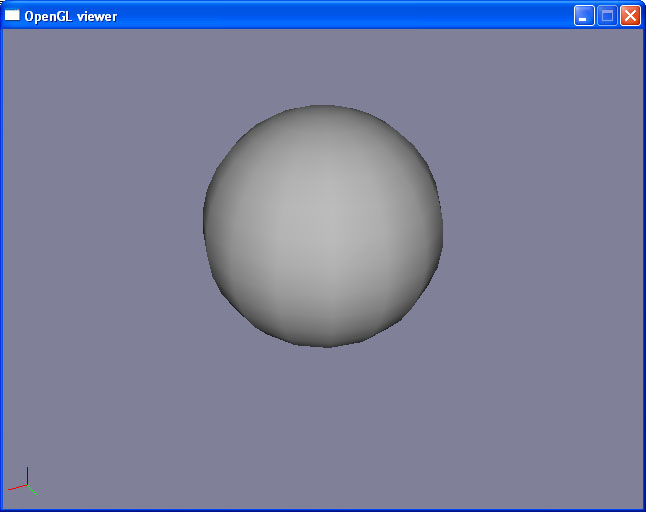
\includegraphics[width=8cm]{pics/helloworld}
\end{center}

The viewer tool reads the contents of the file which in this case
is an ordinary Python file and displays the scene using OpenGL.
When the input file is processed via the viewer tool it is executed
in a special environment where a couple of modules have already been imported.
That's why calling \code{Sphere()} doesn't result in a \exception{NameError}
exception. If you import the relevant modules yourself you can also call
the script without the viewer tool (however, you wouldn't get a visualization
of the scene then). You can also create the above scene directly in a 
Python shell:

\begin{verbatim}
>>> from cgkit.all import *
>>> Sphere()
<cgkit.quadrics.Sphere object at 0x051CC2D0>
\end{verbatim}

The first line imports all you need from cgkit which has to be done
manually now. The second line creates an instance of the
\class{Sphere} class. Usually, each object automatically inserts
itself into the scene, so we don't have to keep the resulting
reference. Now let's create another object:

\begin{verbatim}
>>> b=Box(name="Cube", pos=(1.5,2,0))
>>> listWorld()
Root
+---Cube (Box)
+---Sphere (Sphere)
\end{verbatim}

The first line creates a box object. This time we are passing a couple
of parameters like the object's name and its position and we store the
object in the variable \var{b} so we can manipulate the box afterwards.
The second line calls the \function{listWorld()} function
which prints a tree representation of the current scene.
Now it's time for a little nitpicking, actually the function only displays
the {\em world} (hence its name) and not the entire {\em scene}. The world
is what you see, it stores all 3D objects that have a visual representation
and is part of the scene. The whole scene also contains other objects
such as the timer, animation curves, etc. An object stored in the
scene is called a {\em component} and an object stored in the world
is, well, a {\em world object} (which is also a component as it is also
part of the scene). But back to the example. We have kept a reference to
the box, so let's see what we can do with it:

\begin{verbatim}
>>> b.name = "The Cube"
>>> listWorld()
Root
+---Sphere (Sphere)
+---The Cube (Box)
>>> b.pos
(1.5, 2, 0)
>>> b.pos=vec3(1,0,2)
>>> b.pos
(1, 0, 2)
>>> b.scale
(1, 1, 1)
\end{verbatim}

Every world object has a set of attributes that defines its state.
The exact set of attributes depends on the type of object, but there
are some common attributes that every world object has such as a name or
a position (see chapter \ref{worldobjects} for a reference of the available
world objects together with their attributes).

In the first example, we were only specifying one sphere with its default
attributes, that's why we had some geometry in the scene. But for a 3D scene
to be displayed you usually need two more ingredients: a camera and some 
light. In the above case, a default camera and light source was created
by the viewer tool. In the following example, we specify a complete scene,
including a camera, two colored light sources and a sphere with a material
assigned to it. Create a file "simplescene.py" with the following content:

\begin{verbatim}
TargetCamera(
    pos    = (3,2,2),
    target = (0,0,0)
)

GLPointLight(
    pos       = (3, -1, 2),
    diffuse   = (1, 0.7, 0.2)
)

GLPointLight(
    pos       = (-5, 3, 0),
    diffuse   = (0.2, 0.2, 0.5),
    intensity = 3.0
)

Sphere(
    name      = "My Sphere",
    radius    = 1.0,
    material  = GLMaterial(
                   diffuse = (0.7, 1, 0.7)
                )
)
\end{verbatim}

Display the scene by calling:

\begin{verbatim}
> viewer.py simplescene.py
\end{verbatim}

The result is this:

\begin{center}
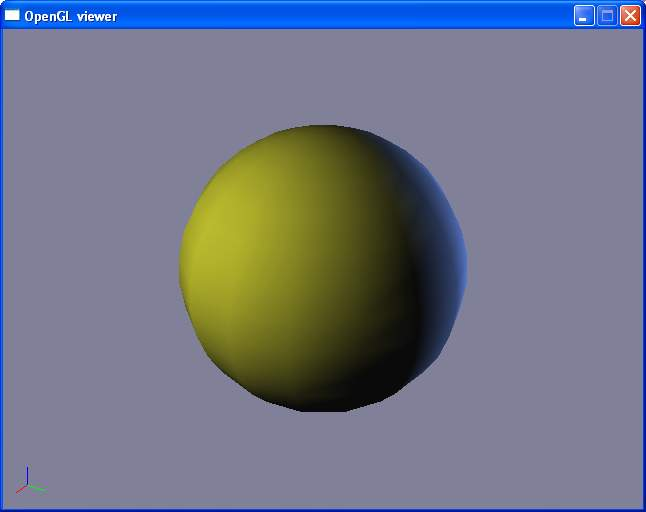
\includegraphics[width=8cm]{pics/simplescene1}
\end{center}

Using the \kbd{Alt} key in combination with the three mouse buttons
you can even navigate around in the scene (if you reach a pole
the camera position will jump around. This is because we are using
a \class{TargetCamera} that always tries to align its local "up"
direction with the global "up" direction, so this type of camera
can't be "upside down").

If you have a RenderMan renderer installed (there are free ones available
such as 3Delight, Aqsis or Pixie) you can try to visualize the above scene
with a different tool:

\begin{verbatim}
> render.py -r<renderer> simplescene.py
\end{verbatim}

\code{<renderer>} has to be replaced with either \code{3delight}, 
\code{aqsis} or \code{pixie}. 
This tool will display the same scene, but this time not using OpenGL but
the specified renderer. The result looks similar than before but is
much smoother:

\begin{center}
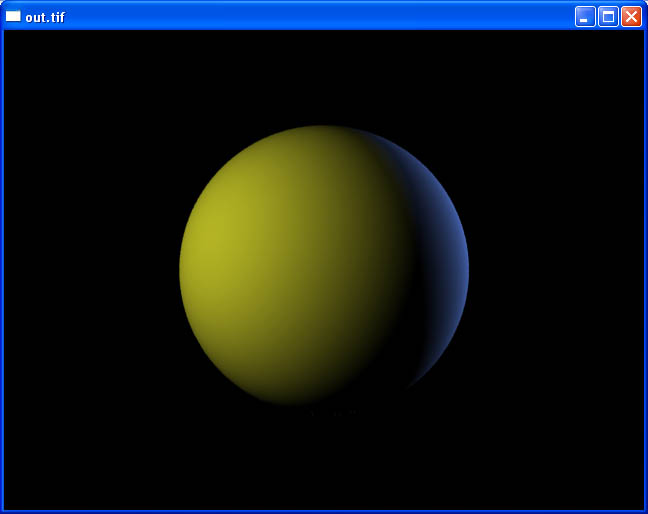
\includegraphics[width=8cm]{pics/simplescene2}
\end{center}

So if you want to create photorealistic images you can use the viewer tool
for previews and the render tool for creating the final image.

%----------------------------------------------------------------------
\section{Components and Slots}

This section gives an overview of the component framework that is the
basis for creating a dynamic 3D scene, i.e. one that is
animated/simulated. The basic mechanism is quite simple to understand
and you might already know it from other graphics packages as it is a
common concept in computer graphics software. The basic idea is to
have some black boxes that can generate values that vary with time and
that can be connected to the attributes we want to be animated. For
example, one such black box could output a three-dimensional vector
which could then be connected to the position of a teapot. If this
black box now produces a series of values that lie on a particular
curve we have an animation of a teapot traveling along that curve.

\begin{center}
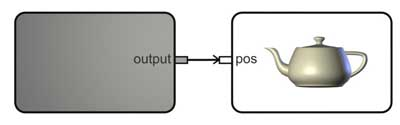
\includegraphics[width=10cm]{pics/slotexample}
\end{center}

In this package those black boxes and the teapot are called {\em
components}. A component is a container for {\em slots} which
represent the input or output values of their respective component. In
the above example, the output value of the "curve point generator" and
the position of the teapot are slots. You can also view them as
"animatable attributes" of an object if they mainly serve as input
values. Most slots can either serve as input value or output
value. However, if the value of a slot is actually computed by some
algorithm then this slot can only be used as output slot.

As a general rule, the actual slot corresponding to an attribute is
obtained by adding the suffix \code{_slot} to the attribute name.
Here is an example where two spheres s1 and s2 are created and
the position of s1 is connected to the position of s2 which means
s2 will always have the same position as s1:

\begin{verbatim}
>>> from cgkit import *
>>> s1=Sphere(pos=(1,2,3))
>>> s2=Sphere(pos=(-1,0,5))
>>> s1.pos
(1, 2, 3)
>>> s2.pos
(-1, 0, 5)

# Connect the positions 
>>> s1.pos_slot.connect(s2.pos_slot)

# Now s2 has the same position as s1
>>> s2.pos
(1, 2, 3)

# Changing the position of s1 will also change the position of s2
>>> s1.pos=vec3(-5,12,42)
>>> s2.pos
(-5, 12, 42)
\end{verbatim}

%----------------------------------------------------------------------
\section{Coordinate systems}

Each world object has a position and orientation in space. This
transformation can be described by a matrix that represents the
object's local coordinate system. The local coordinate system L stored
in each world object is given with respect to its parent coordinate
system which usually is just the world coordinate system unless you
have linked two objects. If you want the local coordinate system with
respect to the world system you have to travel up the transformation
hierarchy and concatenate all local systems (however, you don't have to
do that yourself as a world object already has an attribute 
\var{worldtransform} which does this for you). 

The geometry of a world object is given with respect to the local
coordinate system L. So this is the matrix that's required during
rendering. You get L by calling \method{localTransform()} on the
respective world object.

So far, if you would apply a rotation to an object it would rotate
around the origin or if you would scale the object the center of the
scale would lie in the origin. This is not always the desired behavior
and that's why you can specify a pivot point, or rather, a pivot
transformation or offset transformation P. This transformation is
given with respect to L and is the identity by default. You can get
and set this transformation using the \method{getOffsetTransform()} and
\method{setOffsetTransform()} methods.

The concatenation of L and P is the transformation T ($T=L\cdot
P$). This is what the
\var{transform}, \var{pos}, \var{rot} and \var{scale} slots of a world 
object describe. So if you modify the transform slot you also modify L
whereas P always remains constant, unless you change it explicitly via
\method{setOffsetTransform()}.

\begin{center}
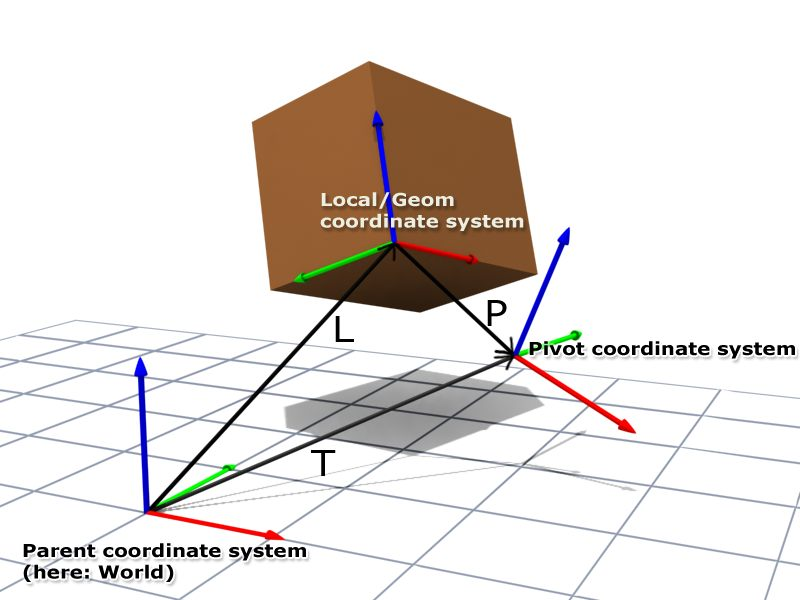
\includegraphics[width=12cm]{pics/coordsys}
\end{center}

Here is a simple code example where you can see the effects when
modifying the different transformations:

\begin{verbatim}
>>> s = Sphere()
>>> s.pos = vec3(1,2,0)
>>> s.pos
<1, 2, 0>
>>> s.setOffsetTransform(mat4().translation(vec3(2,4,7)))
>>> s.pos
<3, 6, 7>
>>> s.pos = vec3(0,0,0)
>>> s.pos
<0, 0, 0>
>>> s.localTransform()
[1, 0, 0, -2]
[0, 1, 0, -4]
[0, 0, 1, -7]
[0, 0, 0, 1]
\end{verbatim}

%---

\chapter{Building \& Installing \label{build}}

% Building and Installing

This chapter provides information about how to build the kit yourself
from the sources. You can skip this chapter if the kit is already
installed on your system or if you are installing binary versions.

%----------------------------------------------------------------------
\section{Building from the sources}

The following instructions will build and install the full version of cgkit.
You can also install the 'light' version by setting the variable 
\code{INSTALL_CGKIT_LIGHT} to \code{True} in your config file (just rename
the file \code{config_template.cfg} to \code{config.cfg} and uncomment the
corresponding line at the top of the file). Except for Python itself, 
installing the light version does not require any additional compiler, tool
or library, you simply have to call 

\begin{verbatim}
> python setup.py install    # that's all for the light version
\end{verbatim}

while being in the root directory of the cgkit sources. For installing
the light version you can skip the remainder of this section, but read
on if you actually want to install the full version.

The steps required to build the full version of the kit are the same
on every platform.  The build process assumes you have the following
tools/libraries installed on your system:

\begin{itemize}
\item \ulink{Boost}{http://www.boost.org/} (v1.31) - Make sure that Boost is
 installed including Boost.Python (e.g. Mac users who are using darwinports
 have to install the "+python" variant).
\item \ulink{SCons}{http://www.scons.org/} (v0.96.1)
\item \ulink{lib3ds}{http://lib3ds.sourceforge.net/} (v1.3.0) - {\bf Optional}. You need this if you want to import/export 3DS files.
\item \ulink{CyberX3D}{http://www.cybergarage.org/vrml/cx3d/cx3dcc/index.html} - {\bf Optional}. You need this if you want to import/export VRML or X3D files.
\item \ulink{OGRE}{http://www.ogre3d.org/} - {\bf Optional}. You need this if you want to use the OGRE-Viewer.
\item \ulink{STLport}{http://www.stlport.com/} - Only required on Windows when
 you want to use OGRE.
\item \ulink{3DxWare SDK}{http://www.3dconnexion.com/sdk.htm} - {\bf Optional} (currently Windows only). You need this if you want to use a SpaceMouse or SpaceBall.
\item \ulink{Wintab Programmer's Kit}{http://www.pointing.com/} - {\bf Optional} (Windows only). You need this if you want to use a tablet (or similar device).
\item \ulink{GloveSDK}{http://www.5dt.com/} - {\bf Optional}. You need this if you want to use a data glove. {\bf Note}: Download the version 2 SDK from the Ultra series, this can also be used with older gloves. You could also use version 1, but some functionality won't be available then.
\end{itemize}

If you have successfully installed the above tools and libraries you
can proceed with building the kit.The first step is to get the cgkit
sources. You can either download the source archive or check out the
latest version from CVS. The following build instructions apply to
both versions.

The package consists of three parts:

\begin{enumerate}
\item A pure C++ library that is independent of Python. This library is
 located in the \file{supportlib} directory.
\item Python wrappers around the above C++ library (using Boost.Python). 
 These wrappers are located in the \file{wrappers} directory.
\item The actual Python package using the wrappers. The package is located
 in the \file{cgkit} directory. The command line tools are in the main 
 directory.
\end{enumerate}

Part 2) and 3) is built and installed via the Python distutils (i.e.
the \file{setup.py} script). But before you can do so, you have to
build the C++ library manually using SCons.

{\bf Building the C++ support library:}

The C++ library is located in the directory \file{supportlib}. The library
uses SCons as its build system. If you have to customize the build process
you can create a file \file{cpp_config.cfg} where you can set some build
variables (e.g. adding search paths for include files). There is a template
file \file{cpp_config_template.cfg} which you can use to create the actual
config file. However, if you have installed every library in standard
directories it may well be that you don't need any config file at all.
Eventually you can build the library by calling \program{scons}:

\begin{verbatim}
> cd supportlib
> # ...create & modify cpp_config.cpp if necessary...
> scons
\end{verbatim}

If everything went fine you can see the result in the \file{lib}
subdirectory (\file{libcore.a} on Linux or \file{core.lib} on Windows).

{\bf Building the Python wrappers:}

The next step is to build and install the Python package. The package
uses the distutils, so you will find the familiar \file{setup.py}
script in the main directory. Customization of the build process can again
be done in a file called \file{config.cfg} which is executed by the setup
script. There is a template file \file{config_template.cfg} which you can
use to create your own config file. After setting up your
configuration you can install the package with the usual procedure:

\begin{verbatim}
> cd ..  # if you were still in the supportlib directory
> python setup.py install
\end{verbatim}

(see the manual \citetitle{Installing Python Modules} in your Python
documentation for more details about the distutils and how to proceed
if you have any special requirements)

Please also have a look at section \ref{externaldeps} for a list of
third-party packages you might have to install before you can use cgkit.
You can check cgkit and its dependencies with the script 
\file{utilities/checkenv.py} that is part of the source archive.
For a more thorough test you can run the unit tests in the \file{unittests}
directory.

A note to developers: You can build the package inplace by calling

\begin{verbatim}
> python setup.py build_ext --inplace
\end{verbatim}

In this case, the resulting binaries will be placed directly in the
\file{cgkit} directory which will then contain the entire package. Use
the \envvar{PYTHONPATH} variable and add the path to the main
directory if you want to use the inplace version from any other
directory.


%---

\chapter{Tools \label{tools}}

% Viewer tool

\section{The interactive viewer tool}

The tool \file{viewer.py} reads one or more files and displays the
scene using a simple OpenGL renderer. It creates events such as
keyboard, mouse or joystick events that can be used by the components
in the scene.

If the environment variable \envvar{VIEWER_DEFAULT_OPTIONS} exists, it
is read and parsed to set the default options. After that the options
in the command line are parsed.

{\bf Usage:}

\begin{verbatim}
viewer.py [options] inputfiles
\end{verbatim}

To exit the viewer press \kbd{Escape} or close the window. How to
navigate in the scene depends on the navigation mode (see option -N).

{\bf Options:}

\begin{description}
\item[\code{-f<int>} / \code{--fps=<int>}] 
Specifies the frame rate that should be tried to maintain while playing
back the scene (default: 30).

\item[\code{-h} / \code{--help}]
Print a help message.

\item[\code{-F} / \code{--full-screen}]
Open a full screen display.

\item[\code{-W<int>} / \code{--width=<int>}]
Specify the width in pixels of the window/screen (default: 640).

\item[\code{-H<int>} / \code{--height=<int>}]
Specify the height in pixels of the window/screen (default: 480). If
no height is specified it is computed based on the width and an aspect
ratio of 4/3.

\item[\code{-v} / \code{--verbose}]
Output info messages.

\item[\code{-p<str>} / \code{--plugin=<str>}]
If the argument specifies a file this file is loaded as a plugin, if it
is a directory, all files in this directory are loaded. You can specify
this option more than once or you can use a comma separated list of names.

You can also set files and paths via the environment variable
\envvar{CGKIT_PLUGIN_PATH}. The files/paths have to be separated either
by ':' or ';'.

\item[\code{-c<str>} / \code{--camera=<str>}]
Select the camera that should be used to view the scene. The argument
is the name of the camera. If no camera is specified the first camera
found in the scene is used.

\item[\code{-b<time>} / \code{--begin=<time>}]
Specify a time or frame where the animation/simulation should be started
(default: 0s). You can add the time unit such as 's' for seconds or 'f'
for frames. Frames are assumed if you don't specify a unit.

\item[\code{-e<time>} / \code{--end=<time>}]
Specify a time or frame where the animation/simulation should be stopped.
You can add the time unit such as 's' for seconds or 'f' for frames. 
Frames are assumed if you don't specify a unit.

\item[\code{-U<axis>} / \code{--up=<axis>}]
Specify the default value for the up axis. The argument may be either
'y' or 'z'.

\item[\code{-O<str>} / \code{--option=<str>}]
Add a global option that will be stored in the scene. The argument should
have the form "name=value". Using this option is equivalent to writing
"Globals( name=value )" in a scene file.

\item[\code{-t} / \code{--set-time}]
Set the starting time directly instead of stepping there from time 0.

\item[\code{-S<str>} / \code{--stereo=<str>}]
Activate stereo display. The argument specifies the method that should be
used to create a stereo image. It can be either \var{vsplit} or \var{glstereo}.

\item[\code{-D<float>} / \code{--eye-distance=<float>}]
Default eye distance for stereo display (default 0.07). This distance
value is used if the camera does not explicitly specify a distance value
(i.e. if it has no attribute \var{eye_distance}).

\item[\code{-B} / \code{--bounding-box}]
Display the bounding boxes.

\item[\code{-P<str>} / \code{--polygon-mode=<str>}]
Specify how polygons should be rendered. Possible values are
\var{fill} (default), \var{line} and \var{point}.

\item[\code{-s<str>} / \code{--save=<str>}]
When this option is specified each frame is saved under the given name
(+ frame number). The extension determines the image format.

\item[\code{-N<str>} / \code{--navigation-mode=<str>}]
Specify which navigation mode to activate. The viewer can emulate the
navigation of a few common 3D packages. Possible values are
\var{Maya} (default), \var{MAX} and \var{Softimage} (case-insensitive).

In Maya mode you navigate by pressing the \kbd{Alt} key in combination
with any of the three mouse buttons. In MAX mode you press the middle
mouse button either alone or in combination with \kbd{Alt} or \kbd{Control}
and \kbd{Alt}. In Softimage mode, only the Softimage Navigation Tool is
emulated (it's as if this tool is permanently active), i.e. you navigate
by using one of the three mouse buttons.

\item[\code{-X} / \code{--disable-spacedevice}]
Disables support for SpaceMouse/SpaceBall. This option can be used if there
are any problems with the driver or initialization takes too long.

\item[\code{-T} / \code{--disable-wintab}]
Disables tablet support. This option can be used if there are any
problems with the driver or initialization takes too long.

\end{description}

{\bf Events:}

The viewer tool generates the following user input events (see the
module \refmodule{cgkit.events} for more details about these events):

\begin{itemize}
\item \code{KEY_PRESS}
\item \code{KEY_RELEASE}
\item \code{LEFT_DOWN}
\item \code{MIDDLE_DOWN}
\item \code{RIGHT_DOWN}
\item \code{MOUSE_BUTTON_DOWN}
\item \code{LEFT_UP}
\item \code{MIDDLE_UP}
\item \code{RIGHT_UP}
\item \code{MOUSE_BUTTON_UP}
\item \code{MOUSE_WHEEL}
\item \code{MOUSE_MOVE}
\item \code{JOYSTICK_AXIS}
\item \code{JOYSTICK_BALL}
\item \code{JOYSTICK_HAT}
\item \code{JOYSTICK_BUTTON_DOWN}
\item \code{JOYSTICK_BUTTON_UP}
\item \code{SPACE_MOTION}
\item \code{SPACE_BUTTON_DOWN}
\item \code{SPACE_BUTTON_UP}
\item \code{SPACE_BUTTON_ZERO}
\item \code{TABLET}
\end{itemize}

{\bf Timing:}

The operations per frame are as follows (in this order):

\begin{enumerate}
\item Render and display the current scene at time $t$
\item Handle events
\item Step frame (i.e. increase the time by $\Delta t$ and signal the
  \code{STEP_FRAME} event)
\item Sync to the specified framerate
\end{enumerate}

% Render tool

\section{The render tool}

The tool \file{render.py} reads one or more files and renders the
scene using a RenderMan renderer. The tool takes care of creating the
RIB files and the shaders, compiling the shaders and launching the 
renderer.

If the environment variable \envvar{RENDER_DEFAULT_OPTIONS} exists, it
is read and parsed to set the default options. After that the options
in the command line are parsed.

{\bf Usage:}

\begin{verbatim}
render.py [options] inputfiles
\end{verbatim}


{\bf Options:}

\begin{description}
\item[\code{-f<int>} / \code{--fps=<int>}] 
Specifies the number of frames per second (default: 30).

\item[\code{-h} / \code{--help}]
Print a help message.

\item[\code{-W<int>} / \code{--width=<int>}]
Specify the width in pixels of the window/screen (default: 640).

\item[\code{-H<int>} / \code{--height=<int>}]
Specify the height in pixels of the window/screen (default: 480). If
no height is specified it is computed based on the width and an aspect
ratio of 4/3.

\item[\code{-v} / \code{--verbose}]
Output info messages.

\item[\code{-p<str>} / \code{--plugin=<str>}]
If the argument specifies a file this file is loaded as a plugin, if it
is a directory, all files in this directory are loaded. You can specify
this option more than once or you can use a comma separated list of names.

You can also set files and paths via the environment variable
\envvar{CGKIT_PLUGIN_PATH}. The files/paths have to be separated either
by ':' or ';'.

\item[\code{-c<str>} / \code{--camera=<str>}]
Select the camera that should be used to view the scene. The argument
is the name of the camera. If no camera is specified the first camera
found in the scene is used.

\item[\code{-b<time>} / \code{--begin=<time>}]
Specify a time or frame where the animation/simulation should be started
(default: 0s). You can add the time unit such as 's' for seconds or 'f'
for frames. Frames are assumed if you don't specify a unit.

\item[\code{-e<time>} / \code{--end=<time>}]
Specify a time or frame where the animation/simulation should be stopped.
You can add the time unit such as 's' for seconds or 'f' for frames. 
Frames are assumed if you don't specify a unit.

\item[\code{-U<axis>} / \code{--up=<axis>}]
Specify the default value for the up axis. The argument may be either
'y' or 'z'.

\item[\code{-O<str>} / \code{--option=<str>}]
Add a global option that will be stored in the scene. The argument should
have the form "name=value". Using this option is equivalent to writing
"Globals( name=value )" in a scene file.

\item[\code{-t} / \code{--set-time}]
Set the starting time directly instead of stepping there from time 0.

\item[\code{-r<str>} / \code{--renderer=<str>}]
Select the renderer to use (you can choose among \code{aqsis},
\code{3delight}, \code{pixie}, \code{prman}, \code{air} and \code{rdc}).

\item[\code{-I<str>} / \code{--include=<str>}]
Add the specified include path to the list of paths used for compiling
the shaders.

\item[\code{-B} / \code{--bake}]
Activate texture baking mode.

\end{description}

{\bf Events:}

The render tool does not generate any user input events.


%---

\chapter{Generic modules \label{modules1}}

\localmoduletable

\section{\module{cgkitinfo} ---
         Release information}

\declaremodule{extension}{cgkit.cgkitinfo}
\modulesynopsis{Provides version information.}

New in version 1.1. This module contains two variables that carry
information about the version of the kit.

\begin{datadesc}{version}
A string containing version information of this release.
\end{datadesc}

\begin{datadesc}{version_info}
A 4-tuple (\var{major}, \var{minor}, \var{micro}, \var{releaselevel})
containing the components of the version number. The first three
values are integers, whereas \var{releaselevel} is a string containing
"cvs", "alpha", "beta" or "final".
\end{datadesc}

\section{\module{cgtypes} ---
         Vectors, matrices and quaternions}

\declaremodule{extension}{cgkit.cgtypes}
\modulesynopsis{Basic types useful for computer graphics.}

This module contains the fundamental types which make working with 3D
data much easier. The types are:

\begin{itemize}
\item vec3 -- a three dimensional vector type to store points, vectors, normals or even colors.
\item vec4 -- a four dimensional vector type to store homogenous points, for example.
\item mat3 -- a 3x3 matrix to store linear transformations.
\item mat4 -- a 4x4 matrix to store affine transformations.
\item quat -- a quaternion type as a specialized way to store rotations.
\end{itemize}

You import all of those types at once with

\begin{verbatim}
from cgkit.cgtypes import *
\end{verbatim}

or you can import them individually like this

\begin{verbatim}
from cgkit.cgtypes import vec3, mat4
\end{verbatim}

In general, you can use those types just as if they were built-in
types which means the mathematical operators can be used and have
their respective meaning. Each type has some additional methods which
are described in the respective documentation.

Here are some examples:

\begin{verbatim}
>>> from cgkit.cgtypes import *
>>> v=vec3(0.5,1.0,-2.5)
>>> print v
(0.5000, 1.0000, -2.5000)
>>> print v.length()
2.73861278753
>>> v=v.normalize()
>>> print v
(0.1826, 0.3651, -0.9129)
>>> print v.length()
1.0
\end{verbatim}

Now let's construct a rotation matrix that rotates points by 90
degrees around the z-axis:

\begin{verbatim}
>>> M=mat4(1).rotate(0.5*math.pi, vec3(0,0,1))
\end{verbatim}

and apply the rotation to the vector (1,0,0) (the x-axis):

\begin{verbatim}
>>> print M*vec3(1,0,0)
(0.0000, 1.0000, 0.0000)
\end{verbatim}

The module contains the following functions:

\begin{funcdesc}{getEpsilon}{}
Return the epsilon threshold which is used for doing comparisons.
\end{funcdesc}

\begin{funcdesc}{setEpsilon}{eps}
Sets a new epsilon threshold and returns the previously set value. Two
values are considered to be equal if their absolute difference is less
than or equal to epsilon.
\end{funcdesc}

\begin{funcdesc}{slerp}{t, q0, q1}
Performs a spherical linear interpolation between two quaternions q0
and q1. For t=0.0 the return value equals q0, for t=1.0 it equals
q1. q0 and q1 must be unit quaternions. \\
New in version 1.1.
\end{funcdesc}

\begin{funcdesc}{squad}{t, a, b, c, d}
Performs a spherical cubic interpolation between quaternion a and d
where quaternion b and c define the shape of the interpolation
curve. For t=0.0 the return value equals a, for t=1.0 it equals d. All
quaternions must be unit quaternions. \\
New in version 1.1.
\end{funcdesc}

%----------------------------------------------------------------------
\input{vec3.tex}

%----------------------------------------------------------------------
\input{vec4.tex}

%----------------------------------------------------------------------
\input{mat3.tex}

%----------------------------------------------------------------------
\input{mat4.tex}

%----------------------------------------------------------------------
\input{quat.tex}

\section{\module{ri} ---
         RenderMan binding}

\declaremodule{extension}{cgkit.ri}
\modulesynopsis{RenderMan binding}

The RenderMan\textsuperscript{\textregistered} interface is an API
that is used to communicate a 3D scene description (which includes 3D
geometry, light sources, a camera description, etc) to a renderer
which will produce a 2D image of that scene. The API itself is
independent of a particular renderer and can be used for a whole bunch
of renderers, where each could use entirely different rendering
algorithms. There are some excellent renderers freely available, such
as \ulink{3Delight}{http://www.3delight.com/} or the Open Source renderer 
\ulink{Aqsis}{http://www.aqsis.com/} or
\ulink{Pixie}{http://pixie.sourceforge.net/}. On the
commercial side, the most popular renderers are Pixar's
\ulink{Photorealistic RenderMan}{http://www.pixar.com/} (PRMan), 
\ulink{RenderDotC}{http://www.dotcsw.com/} and 
\ulink{AIR}{http://www.sitexgraphics.com/}. 
The RenderMan interface was
created by Pixar and the official specification can be downloaded from
their site.

This document is not an introduction to the RenderMan interface
itself, it just explains the usage of this particular Python
binding. The binding was written to be compliant to v3.2 of Pixar's
RenderMan Interface specification. However, it also supports some
newer features such as string handles for light sources or object
instances.

\subsection{Using the API}

It is safe to import the module using 

\begin{verbatim}
from cgkit.ri import * 
\end{verbatim}

All the functions that get imported start with the prefix \code{Ri},
all constants start with \code{RI_} or \code{RIE_}, so you probably
won't get into a naming conflict.

After importing the module this way you can use the functions just as
you're used to from the C API (well, almost).

\begin{verbatim}
from cgkit.ri import *

RiBegin(RI_NULL)
RiWorldBegin()
RiSurface("plastic")
RiSphere(1,-1,1,360)
RiWorldEnd()
RiEnd()
\end{verbatim}

The parameter to \function{RiBegin()} determines where the output is
directed to. You can pass one of the following:

\begin{itemize}
\item \code{RI_NULL} or an empty string: The RIB stream will be written to 
stdout. 
\item A name that contains the suffix \code{".rib"} (case insensitive): 
A file with the given name is created and the RIB stream is written into it. 
\item A name that contains the suffix \code{".rib.gz"} (case insensitive):
Same as before, but the stream is compressed. The result is the same as if you
would output a RIB file and then compress it using gzip.  
\item A name without the suffix \code{".rib"} or \code{".rib.gz"}: The name
is supposed to be an external program that reads RIB from stdin. 
The program is launched and the RIB stream is piped into it.
\end{itemize}

%-----------
\subsection{Online documentation}

Every function has an associated doc string that includes a short
description of the function, some information about what parameters
the function expects and an example how the function is called.

Example (inside an interactive Python session):

\begin{verbatim}
>>> from ri import *
>>> help(RiPatch)
RiPatch(type, paramlist)

    type is one of RI_BILINEAR (4 vertices) or RI_BICUBIC (16 vertices).

    Number of array elements for primitive variables:
    -------------------------------------------------
    constant: 1              varying: 4
    uniform:  1              vertex:  4/16 (depends on type)

    Example: RiPatch(RI_BILINEAR, [0,0,0, 1,0,0, 0,1,0, 1,1,0])
\end{verbatim}

or from the shell (outside the Python shell):

\begin{verbatim}
> pydoc ri.RiCropWindow

Python Library Documentation: function RiCropWindow in ri

RiCropWindow(left, right, bottom, top)
    Specify a subwindow to render.

    The values each lie between 0 and 1.

    Example: RiCropWindow(0.0, 1.0 , 0.0, 1.0)  (renders the entire frame)
             RiCropWindow(0.5, 1.0 , 0.0, 0.5)  (renders the top right quarter)
\end{verbatim}

%-----------
\subsection{Differences between the C and Python API}

The Python RenderMan binding is rather close to the C API, however
there are some minor differences you should know about.

{\bf Types}

In this binding typing is not as strict as in the C API. The type names
RtBoolean, RtInt, RtFloat, etc. don't exist in this API, you just use
the corresponding Python types (for booleans the module defines the
constants \code{RI_TRUE} and \code{RI_FALSE}).

Wherever the API expects vector types (RtPoint, RtMatrix, RtBound,
RtBasis) you can use any value that can be interpreted as a sequence
of the corresponding number of scalar values. These can be lists,
tuples or your own class that can be used as a sequence.

It is also possible to use nested sequences instead of flat ones. For
example, you can specify a matrix as a list of 16 values or as a list
of four 4-tuples. The following two calls are identical:

\begin{verbatim}
RiConcatTransform([2,0,0,0, 0,2,0,0, 0,0,2,0, 0,0,0,1]) 

RiConcatTransform([[2,0,0,0], [0,2,0,0], [0,0,2,0], [0,0,0,1]])
\end{verbatim}

{\bf Parameter lists}

When passing parameter lists you have to know the following points:

\begin{itemize}
\item In C parameter lists have to be terminated with \code{RI_NULL}. In Python
this is not necessary, the functions can determine the number of
arguments themselves. However, adding \code{RI_NULL} at the end of the list
will not generate an error. For example, if you are porting C code to
Python you don't have to change those calls. So the following two
calls are both valid:

\begin{verbatim}
RiSurface("plastic", "kd", 0.6, "ks", 0.4)
RiSurface("plastic", "kd", 0.6, "ks", 0.4, RI_NULL) 
\end{verbatim}

\item The tokens inside the parameter list have to be declared (either
inline or using \function{RiDeclare}), otherwise an error is
generated. Standard tokens (like \code{RI_P}, \code{RI_CS}, ...) are
already pre-declared.

\item Parameter lists can be specified in several ways. The first way is the
familiar one you already know from the C API, that is, the token and
the value are each an individual parameter:

\begin{verbatim}
RiSurface("plastic", "kd", 0.6, "ks", 0.4) 
\end{verbatim}

Alternatively, you can use keyword arguments: 

\begin{verbatim}
RiSurface("plastic", kd=0.6, ks=0.4) 
\end{verbatim}

But note that you can't use inline declarations using keyword
arguments. Instead you have to previously declare those variables
using \function{RiDeclare}. Also, you can't use keyword arguments if
the token is a reserved Python keyword (like the standard \code{"from"}
parameter).  The third way to specify the parameter list is to provide
a dictionary including the token/value pairs:

\begin{verbatim}
RiSurface("plastic", {"kd":0.6, "ks":0.4}) 
\end{verbatim}

This is useful if you generate the parameter list on the fly in your program.
\end{itemize}

{\bf Arrays}

In the C API functions that take arrays as arguments usually take the
length of the array as a parameter as well. This is not necessary in
the Python binding. You only have to provide the array, the length can
be determined by the function.

For example, in C you might write: 

\begin{verbatim}
RtPoint points[4] = {0,1,0, 0,1,1, 0,0,1, 0,0,0};
RiPolygon(4, RI_P, (RtPointer)points, RI_NULL); 
\end{verbatim}

The number of points has to be specified explicitly. In Python
however, this call could look like this:

\begin{verbatim}
points = [0,1,0, 0,1,1, 0,0,1, 0,0,0]
RiPolygon(RI_P, points) 
\end{verbatim}

The functions that are affected by this rule are: 

\begin{verbatim}
RiBlobby()
RiColorSamples()
RiCurves()
RiGeneralPolygon()
RiMotionBegin()
RiPoints()
RiPointsGeneralPolygons()
RiPointsPolygons()
RiPolygon()
RiSubdivisionMesh()
RiTransformPoints()
RiTrimCurve()
\end{verbatim}

{\bf User defined functions}

Some RenderMan functions allow to take user defined functions as input
which will be used during rendering. Since this implementation only
outputs RIB streams it is not possible to use your own functions in
these cases, instead you always have to use one of the predefined
functions.
 
{\em Filter functions}

It is not possible to use your own filter functions, you have to use
one of the predefined filters:

\begin{itemize}
\item RiGaussianFilter 
\item RiBoxFilter 
\item RiTriangleFilter 
\item RiSincFilter 
\item RiCatmullRomFilter 
\end{itemize}

{\em Procedurals}

It is not possible to use your own procedurals directly in the RIB
generating program, you can only use one of the predefined procedural
primitives:

\begin{itemize}
\item RiProcDelayedReadArchive 
\item RiProcRunProgram 
\item RiProcDynamicLoad
\end{itemize}

However, this is not really a restriction since you always can use
RiProcRunProgram to invoke your Python program that generates
geometry.

{\bf Extended transformation functions}

The transformation functions \function{RiTranslate()}, \function{RiRotate()}, 
\function{RiScale()} and \function{RiSkew()} have been extended in a way 
that is not part of the official
spec. Each of these functions takes one or two vectors as input which
usually are provided as 3 separate scalar values, like the axis of a
rotation for example:

\begin{verbatim}
RiRotate(45, 0,0,1) 
\end{verbatim}

Now in this implementation you can choose to provide such vectors as
sequences of 3 scalar values:

\begin{verbatim}
RiRotate(45, [0,0,1]) 

axis = vec3(0,0,1)
RiRotate(45, axis)
\end{verbatim}

{\bf Empty stubs}

All the functions do what they are supposed to do (well, hopefully ;)
except for the function RiTransformPoints(). This function is defined
but it does nothing, it is only an empty stub (since the module only
outputs RIB and does not maintain transformation matrices).

%-----------
\subsection{Implementation specific options}

There is currently one option that is specific to this RenderMan
binding and that won't produce any RIB call but will control what gets
written to the output stream:

\begin{funcdesc}{RiOption}{RI_RIBOUTPUT, RI_VERSION, 0}
If this option is set to 0 directly after \function{RiBegin()} is
called, then no \code{"version"} call will be generated in the RIB stream
(default is 1).\\
New in version 1.1.
\end{funcdesc}

%-----------
\subsection{Error handling}

Besides the three standard error handlers RiErrorIgnore, RiErrorPrint
(default) and RiErrorAbort the module provides an additional error
handler called RiErrorException. Whenever an error occurs
RiErrorException raises the exception \exception{RIException}.

If you install a new error handler with \function{RiErrorHandler()}
only the three standard error handlers will produce an output in the
RIB stream, if you install RiErrorException or your own handler then
the handler is installed but no RIB output is produced.

The module does some error checking, however there are still quite a
bit of possible error cases that are not reported. For example, the
module checks if parameters are declared, but it is not checked if you
provide the correct number of values. In general, the module also does
not check if a function call is valid in a given state (e.g. the
module won't generate an error if you call \function{RiFormat()}
inside a world block).



\section{\module{riutil} ---
         RenderMan utilities}

\declaremodule{extension}{cgkit.riutil}
\modulesynopsis{RenderMan utility functions}

\begin{funcdesc}{RiuArrow}{height=1.0, thickness=0.1, headheight=0.2, headscale=1.7}
\end{funcdesc}

\begin{funcdesc}{RiuCoordSystem}{thickness=0.06, shader="matte"}
\end{funcdesc}

\begin{funcdesc}{RiuDefaultHeader}{}
Outputs a default header into the RIB stream. This function can be
called right after \function{RiBegin()} to write the following
information into the RIB stream:

\begin{verbatim}
##RenderMan RIB-Structure 1.1
##Creator <Filename>
##CreationDate <Date>
##For <User>
\end{verbatim}

The "For" information is left out if the user name cannot be determined.
\end{funcdesc}

\begin{funcdesc}{RiuGrid}{thickness=0.02, cells=6, shader="matte", color=(0.9, 0.9, 0.9)}
Outputs a grid primitive. \var{thickness} determines the thickness of the
grid lines and \var{cells} the number of gridlines. The grid lies on the XY
plane and is centered at the origin. The grid spacing is 1 unit. The
grid uses the given shader and color.

\begin{center}
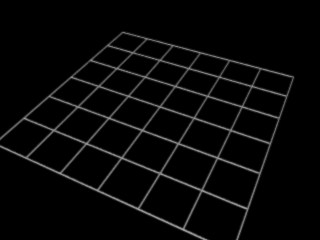
\includegraphics[width=6cm]{pics/grid}
\end{center}
\end{funcdesc}

\section{\module{noise} ---
         Noise functions}

\declaremodule{extension}{cgkit.noise}
\modulesynopsis{A set of basic noise functions}

\begin{funcdesc}{noise}{x[, y[, z[,t]]]}
Returns a noise value (Perlin) in the range from 0 to 1. The arguments
can be up to 4 floating point values or a sequence with up to 4
floating point values (e.g. a \class{vec3} or a \class{vec4}) with an
optional time value. The return value is a pseudo random number in the
range from 0 to 1. Due to the nature of this noise implementation
(gradient noise) the return value at integer lattice points is always 0.5.

As an example, here is a 2D slice (the grid shows the integer lattice):

\begin{center}
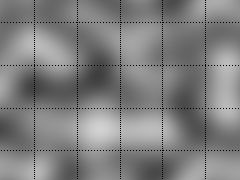
\includegraphics[width=6cm]{pics/noise}
\end{center}

\note{The actual function call depends on the number of arguments, so
calling noise(x,y) is not the same as calling noise(x,y,0). The former
case is a true 2D noise whereas the latter is 3D. The same difference
exists between 3D and 4D.}
\end{funcdesc}

\begin{funcdesc}{snoise}{x[, y[, z[,t]]]}
Returns a signed noise value (Perlin) in the range from -1 to 1. A
call to \code{snoise(args)} is equivalent to \code{2*noise(args)-1}.
\end{funcdesc}

\begin{funcdesc}{pnoise}{point[, t], period[, tperiod]}
Periodic noise function. Basically this is the same as
\function{noise()} but with a periodic return value: \function{pnoise(point)} =
\function{pnoise(point+period)}. The time value can be either part of the point
or it can be specified separately. The point and period must always
have the same dimension. The return value is in the range from 0 to 1.
\end{funcdesc}

\begin{funcdesc}{spnoise}{point[, t], period[, tperiod]}
Signed periodic noise function. The return value is in the range from
-1 to 1. A call to \code{spnoise(args)} is equivalent to 
\code{2*pnoise(args)-1}.
\end{funcdesc}

\begin{funcdesc}{cellnoise}{x[, y[, z[,t]]]}
Returns a pseudo random number which is constant between integer
lattice points. The return value is in the range from 0 to 1.

As an example, here is a 2D slice (the grid shows the integer lattice):

\begin{center}
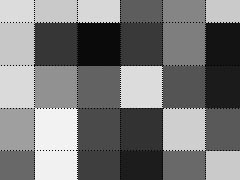
\includegraphics[width=6cm]{pics/cellnoise}
\end{center}
\end{funcdesc}

\begin{funcdesc}{scellnoise}{x[, y[, z[,t]]]}
Signed cell noise. The return value is in the range from -1 to 1. A
call to \code{scellnoise(args)} is equivalent to \code{2*cellnoise(args)-1}.
\end{funcdesc}

\begin{funcdesc}{fBm}{point, octaves, lacunarity=2.0, gain=0.5}
Fractional Brownian motion. The argument point must be a sequence of
either 2 or 3 float values (e.g. a \class{vec3}). This function is a sum of
noise values with different frequencies and amplitudes and is
equivalent to the following code:

\begin{verbatim}
sum = 0.0
amp = 1.0
for i in range(octaves):
    sum += amp*snoise(point)
    amp *= gain
    point *= lacunarity
\end{verbatim}

The return value is in the range from 0 to 1.

As an example, here is a 2D slice (the grid shows the integer lattice):

\begin{center}
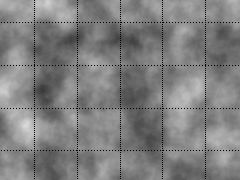
\includegraphics[width=6cm]{pics/fbm}
\end{center}
\end{funcdesc}

\begin{funcdesc}{turbulence}{point, octaves, lacunarity=2.0, gain=0.5}
The code of the turbulence function is very similar to \function{fBm()}. The
difference is that it sums up \code{abs(snoise())} instead of \code{noise()}. 
However, the return value is in the range from 0 to 1.

As an example, here is a 2D slice (the grid shows the integer lattice):

\begin{center}
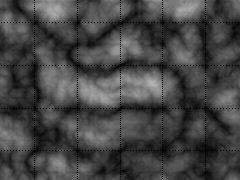
\includegraphics[width=6cm]{pics/turbulence}
\end{center}
\end{funcdesc}


All of the above functions have a vector version that take the same
input parameters but return a vector as result. The output always has
the same dimension than the input. If the time value is specified
separately it does not count to the dimension. For example a call to
\code{vnoise((x,y,z))} returns a \class{vec3}, just as a call to
\code{vnoise((x,y,z),t)}. However, a call to \code{vnoise((x,y,z,t))} 
returns a \class{vec4}.

\begin{funcdesc}{vnoise}{x[, y[, z[,t]]]}
See \function{noise()}.
\end{funcdesc}

\begin{funcdesc}{vsnoise}{x[, y[, z[,t]]]}
See \function{snoise()}.
\end{funcdesc}

\begin{funcdesc}{vpnoise}{point[, t], period[, tperiod]}
See \function{pnoise()}.
\end{funcdesc}

\begin{funcdesc}{vspnoise}{point[, t], period[, tperiod]}
See \function{spnoise()}.
\end{funcdesc}

\begin{funcdesc}{vcellnoise}{x[, y[, z[,t]]]}
See \function{cellnoise()}.
\end{funcdesc}

\begin{funcdesc}{vscellnoise}{x[, y[, z[,t]]]}
See \function{scellnoise()}.
\end{funcdesc}

\begin{funcdesc}{vfBm}{point, octaves, lacunarity=2.0, gain=0.5}
See \function{fBm()}.
\end{funcdesc}

\begin{funcdesc}{vturbulence}{point, octaves, lacunarity=2.0, gain=0.5}
See \function{turbulence()}.
\end{funcdesc}

\section{\module{sl} ---
         RenderMan Shading Language functionality}

\declaremodule{extension}{cgkit.sl}
\modulesynopsis{Provides the same functions than the RenderMan Shading Language}

This module provides some of the functionality from the RenderMan
Shading Language. Those functions that require an actual rendering
context (surfaces, light sources, etc.) are not supported.

Most of the functions can be used just like in the Shading
Language. An exception are those functions whose return type is
dependant on the context as it is the case with \function{random()} or
\function{noise()}. Here, those functions have to be prepended with the 
return type, for example \function{float_random()} or 
\function{point_noise()} (that is, the cast is part of the name).

%----
\subsection{Constants}

\begin{datadesc}{PI}
This is the same as \code{math.pi}.
\end{datadesc}

%-----
\subsection{Math functions}

\begin{funcdesc}{abs}{x}
Returns the absolute value of its argument. This is just the builtin
\function{abs()} function.
\end{funcdesc}

\begin{funcdesc}{acos}{a}
Returns the arc cosine. This function is imported from the
\module{math} module.
\end{funcdesc}

\begin{funcdesc}{asin}{a}
Returns the arc sine. This function is imported from the \module{math} module.
\end{funcdesc}

\begin{funcdesc}{atan}{y[, x]}
Returns the arc tangent. With one argument \function{math.atan()} is
called, with two arguments \function{math.atan2()} is called.
\end{funcdesc}

\begin{funcdesc}{ceil}{x}
Returns the largest integer not greater than \var{x}. This function is
imported from the \module{math} module.
\end{funcdesc}

\begin{funcdesc}{clamp}{x, min, max}
Returns \var{min} if \var{x} < \var{min}, \var{max} if \var{x} > \var{max}, 
otherwise \var{x}.
\end{funcdesc}

\begin{funcdesc}{color_cellnoise}{p}
Returns a color value (actually a \class{vec3}) whose value is a (pseudo)
random function of its arguments. The return value is constant between
integer lattice points.
\end{funcdesc}

\begin{funcdesc}{color_noise}{p}
Returns a color value (actually a \class{vec3}) whose value is a (pseudo)
random function of its arguments.
\end{funcdesc}

\begin{funcdesc}{color_pnoise}{p, period}
Returns a color value (actually a \class{vec3}) whose value is a periodic
(pseudo) random function of its arguments.
\end{funcdesc}

\begin{funcdesc}{color_random}{}
Return a color whose componenets are a random number between 0 and
1. The function actually returns a \class{vec3}.
\end{funcdesc}

\begin{funcdesc}{cos}{a}
Returns the cosine. This function is imported from the \module{math} module.
\end{funcdesc}

\begin{funcdesc}{degrees}{rad}
Converts from radians to degrees.
\end{funcdesc}

\begin{funcdesc}{exp}{x}
Returns \code{pow(e,x)}. This function is imported from the
\module{math} module.
\end{funcdesc}

\begin{funcdesc}{float_cellnoise}{p}
Returns a float value which is a (pseudo) random function of its
arguments. The return value is constant between integer lattice
points. This function is imported from the \module{noise} module.
\end{funcdesc}

\begin{funcdesc}{float_noise}{p}
Returns a float value which is a (pseudo) random function of its
arguments. This function is imported from the \module{noise} module.
\end{funcdesc}

\begin{funcdesc}{float_pnoise}{p, period}
Returns a float value which is a periodic (pseudo) random function of
its arguments. This function is imported from the \module{noise} module.
\end{funcdesc}

\begin{funcdesc}{float_random}{}
Return a random number between 0 and 1. This call is equivalent to
\function{random.random()}.
\end{funcdesc}

\begin{funcdesc}{floor}{x}
Returns the smallest integer not smaller than \var{x}. This function is
imported from the \module{math} module.
\end{funcdesc}

\begin{funcdesc}{inversesqrt}{x}
Returns \code{1/sqrt(x)}.
\end{funcdesc}

\begin{funcdesc}{log}{x[, base]}
Returns the natural logarithm of \var{x} (the same as
\function{math.log}) or the logarithm to the specified base.
\end{funcdesc}

\begin{funcdesc}{max}{a, b, ...}
Returns the argument with maximum value. This is just the builtin
\function{max()} function.
\end{funcdesc}

\begin{funcdesc}{min}{a, b, ...}
Returns the argument with minimum value. This is just the builtin 
\function{min()} function.
\end{funcdesc}

\begin{funcdesc}{mix}{val0, val1, t}
For \var{t}=0 the value \var{val0} is returned, for \var{t}=1 the value 
\var{val1} is returned. For values of \var{t} between 0 and 1 a linearly 
interpolated value is returned.
\end{funcdesc}

\begin{funcdesc}{mod}{a, b}
Returns \code{a\%b}. This is just an equivalent for the \%-operator.
\end{funcdesc}

\begin{funcdesc}{point_cellnoise}{p}
Returns a point (as a \class{vec3}) whose value is a (pseudo) random
function of its arguments. The return value is constant between
integer lattice points.
\end{funcdesc}

\begin{funcdesc}{point_noise}{p}
Returns a point (as a \class{vec3}) whose value is a (pseudo) random function
of its arguments.
\end{funcdesc}

\begin{funcdesc}{point_pnoise}{p, period}
Returns a point (as a \class{vec3}) whose value is a periodic (pseudo) random
function of its arguments.
\end{funcdesc}

\begin{funcdesc}{point_random}{}
Return a point (a \class{vec3}) whose componenets are a random number between
0 and 1.
\end{funcdesc}

\begin{funcdesc}{pow}{x, y}
Returns x**y. This function is imported from the \module{math} module.
\end{funcdesc}

\begin{funcdesc}{radians}{deg}
Converts from degrees to radians.
\end{funcdesc}

\begin{funcdesc}{round}{deg}
Returns the integer closest to \var{x}. This is just the builtin 
\function{round()} function.
\end{funcdesc}

\begin{funcdesc}{sign}{x}
Returns -1 with a negative argument, +1 with a positive argument, and
0 if its argument is zero.
\end{funcdesc}

\begin{funcdesc}{sin}{a}
Returns the sine. This function is imported from the \module{math} module.
\end{funcdesc}

\begin{funcdesc}{smoothstep}{min, max, value}
Returns 0 if \var{value} < \var{min}, 1 if \var{value} > \var{max},
and performs a smooth Hermite interpolation between 0 and 1 in the
interval \var{min} to \var{max}.
\end{funcdesc}

\begin{funcdesc}{spline}{t, controlpoints}
Fits a spline to the control points given and returns the value at \var{t}
which ranges from 0 to 1. At least four control points must always be
given.
\end{funcdesc}

\begin{funcdesc}{sqrt}{x}
Returns the square root. This function is imported from the \module{math}
module.
\end{funcdesc}

\begin{funcdesc}{step}{min, x}
Returns 0 if \var{x} < \var{min}, otherwise 1.
\end{funcdesc}

\begin{funcdesc}{tan}{a}
Returns the tangent. This function is imported from the \module{math} module.
\end{funcdesc}

\begin{funcdesc}{tan}{a}
Returns the tangent. This function is imported from the \module{math} module.
\end{funcdesc}

\begin{funcdesc}{vector_cellnoise}{p}
Returns a vector (as a \class{vec3}) whose value is a (pseudo) random function
of its arguments. The return value is constant between integer lattice
points.
\end{funcdesc}

\begin{funcdesc}{vector_noise}{p}
Returns a vector (as a \class{vec3}) whose value is a (pseudo) random function
of its arguments.
\end{funcdesc}

\begin{funcdesc}{vector_pnoise}{p, period}
Returns a vector (as a \class{vec3}) whose value is a periodic (pseudo) random
function of its arguments.
\end{funcdesc}

%-----
\subsection{Geometric functions}

\begin{funcdesc}{distance}{p1, p2}
Returns the distance between two points. The arguments should be of type 
\class{vec3}.
\end{funcdesc}

\begin{funcdesc}{faceforward}{N, I, Nref}
Flips \var{N} so that it faces in the direction opposite to \var{I}. 

\note{In contrast to the Shading Language \var{Nref} is not optional.}
\end{funcdesc}

\begin{funcdesc}{length}{v}
Returns the length of a vector. This is equivalent to calling 
\method{v.length()}.
\end{funcdesc}

\begin{funcdesc}{normalize}{v}
Returns a unit vector in the direction of \var{v}. This is equivalent to
calling \method{v.normalize()}.
\end{funcdesc}

\begin{funcdesc}{ptlined}{p0, p1, q}
Returns the distance between point \var{q} and the line segment \var{p0},
\var{p1}. The arguments should be of type \class{vec3}.
\end{funcdesc}

\begin{funcdesc}{reflect}{I, N}
Returns the reflection vector given an incident direction \var{I} and a
normal vector \var{N}. This is equivalent to calling \method{I.reflect(N)}.
\end{funcdesc}

\begin{funcdesc}{refract}{I, N, eta}
Returns the transmitted vector given an incident direction \var{I},
the normal vector \var{N} and the relative index of refraction
\var{eta}. This is equivalent to calling \method{I.refract(N, eta)}.
\end{funcdesc}

\begin{funcdesc}{xcomp}{p}
Return the x component of \var{p}. This is equivalent to \code{p.x}.
\end{funcdesc}

\begin{funcdesc}{ycomp}{p}
Return the y component of \var{p}. This is equivalent to \code{p.y}.
\end{funcdesc}

\begin{funcdesc}{zcomp}{p}
Return the z component of \var{p}. This is equivalent to \code{p.z}.
\end{funcdesc}

\begin{funcdesc}{setxcomp}{p, x}
Set the x component of \var{p}. This is equivalent to \code{p.x = x}.
\end{funcdesc}

\begin{funcdesc}{setycomp}{p, y}
Set the y component of \var{p}. This is equivalent to \code{p.y = y}.
\end{funcdesc}

\begin{funcdesc}{setzcomp}{p, z}
Set the z component of \var{p}. This is equivalent to \code{p.z = z}.
\end{funcdesc}

\begin{funcdesc}{comp}{c, index}
Get an individual color component. This is equivalent to \code{c[index]}.
\end{funcdesc}

\begin{funcdesc}{setcomp}{c, index, value}
Set an individual color component. This is equivalent to 
\code{c[index] = value}.
\end{funcdesc}

%-----
\subsection{String functions}

\begin{funcdesc}{concat}{str1, ..., strn}
Returns a concatenated string.
\end{funcdesc}

\begin{funcdesc}{format}{pattern, val1, val2, ..., valn}
Returns a formatted string (similar to the C function
\cfunction{sprintf()}). Any occurance of the character \% followed by a
letter is replaced by a value. In this implementation it doesn't
matter what letter you are actually using (in the Shading Language it
would be \%f for floats, \%p for points, vectors or normals, \%c for
colors, \%m for matrices and \%s for strings).
\end{funcdesc}

\begin{funcdesc}{match}{pattern, subject}
String pattern matching.
\end{funcdesc}

\begin{funcdesc}{printf}{pattern, val1, val2, ..., valn}
Prints the values of the specified variables. Any occurance of the
character \% followed by a letter is replaced by a value. In this
implementation it doesn't matter what letter you are actually using (in
the Shading Language it would be \%f for floats, \%p for points, vectors
or normals, \%c for colors, \%m for matrices and \%s for strings).
\end{funcdesc}

%-----
\subsection{Unsupported functions}

The following functions are not supported by this module:

\begin{itemize}
\item \cfunction{Du()}
\item \cfunction{Dv()}
\item \cfunction{Deriv()}
\item \cfunction{filterstep()}
\end{itemize}

\begin{itemize}
\item \cfunction{area()}
\item \cfunction{calculatenormal()}
\item \cfunction{depth()}
\item \cfunction{fresnel()}
\item \cfunction{transform()}
\item \cfunction{vtransform()}
\item \cfunction{ntransform()}
\end{itemize}

\begin{itemize}
\item \cfunction{ambient()}
\item \cfunction{diffuse()}
\item \cfunction{phong()}
\item \cfunction{specular()}
\item \cfunction{specularbrdf()}
\item \cfunction{trace()}
\end{itemize}

\begin{itemize}
\item \cfunction{environment()}
\item \cfunction{shadow()}
\item \cfunction{texture()}
\item \cfunction{textureinfo()}
\end{itemize}

\begin{itemize}
\item \cfunction{atmosphere()}
\item \cfunction{displacement()}
\item \cfunction{incident()}
\item \cfunction{lightsource()}
\item \cfunction{opposite()}
\item \cfunction{surface()}
\end{itemize}

\begin{itemize}
\item \cfunction{attribute()}
\item \cfunction{option()}
\item \cfunction{rendererinfo()}
\end{itemize}

\section{\module{sltokenize} ---
          Tokenizer for the RenderMan Shading Language}

\declaremodule{extension}{cgkit.sltokenize}
\modulesynopsis{Tokenizer for the RenderMan Shading Language}

This module provides a lexical scanner for the RenderMan Shading
Language. You use it in the same way as the Python tokenize module is
used.

\begin{funcdesc}{tokenize}{readline, tokeneater}
Reads an input stream and creates tokens. The first parameter,
\var{readline}, must be a callable object which provides the same interface
as the \method{readline()} method of built-in file objects. Each call to the
function should return one line of input as a string.

The second parameter, \var{tokeneater}, must also be a callable
object. It is called with six parameters: the token type, the token
string, a tuple (srow, scol) specifying the row and column where the
token begins in the source, a tuple (erow, ecol) giving the ending
position of the token, the line on which the token was found and the
filename of the current file.

The token type can be one of 

\begin{itemize}
\item \code{WHITESPACE}: This is a series of blanks and/or tabs. 
\item \code{NAME}: A valid identifier name or keyword. 
\item \code{NUMBER}: An integer or float. 
\item \code{STRING}: A string enclosed in '"'. 
\item \code{NEWLINE}: A newline character. 
\item \code{OPERATOR}: An operator such as '+', '-', '!', '==', '!=', etc. 
\item \code{CHARACTER}: A single character that doesn't fit anything else. 
\item \code{TYPE}: A Shading Language type (float, point, vector, normal, matrix, color) 
\end{itemize}

By default, the filename argument is an empty string. It will only be
the actual filename if you provide a preprocessed file stream as input
(so you should first run \code{cpp} on any shader). The tokenizer
actually expects preprocessed data as it does not handle comments.
\end{funcdesc}

\section{\module{slparams} ---
          Extracting RenderMan Shader parameters}
\label{slparams}

\declaremodule{extension}{cgkit.slparams}
\modulesynopsis{Extracting RenderMan Shader parameters}

This module can be used to extract the parameters of a RenderMan
shader either from the shader source file or from the compiled shader.
To read parameters from a compiled shader it is necessary that the renderer
package is installed that was used to compile the shader. Currently, the
following renderers are supported:

\begin{itemize}
  \item 3Delight 
  \item Aqsis
  \item Pixie
  \item PRMan
\end{itemize}

Other renderers can be added at runtime (see the \module{sloargs} module).

\begin{funcdesc}{slparams}{slfile, cpp=None, cpperrstream=sys.stderr, includedirs=None, defines=None}
Extracts the shader parameters from a Shading Language source file. 

The argument \var{slfile} is either the name of a compiled shader, the
name of the shader source file (*.sl) or a file-like object that provides the
shader sources.

\var{cpp} determines how the shader source is preprocessed. It can be
either a string containing the name of an external preprocessor tool
(such as \code{cpp}) that must take the file name as parameter and
dump the preprocessed output to stdout. If the preprocessor does not
produce any data a \exception{PreprocessorNotFound} exception is
thrown. The error stream of the preprocessor is written to the object
that is specified by \var{cpperrstream} which must have a
\method{write()} method. If \var{cpperrstream} is \code{None}, the error 
stream is ignored. \var{cpp} can also be a callable object that takes a
filename as input and returns the filtered contents as a string. If
\var{cpp} is \code{None} a simple internal preprocessor based on the 
\module{simplecpp} module is used.

\var{includedirs} is a list of strings that contain directories where to 
look for include files. \var{defines} is a list of tuples (\var{name},
\var{value}) that specify the predefined symbols to use.

The function returns a list of shader info objects. These objects have
four attributes:
    
\begin{itemize}
  \item \var{type}: The type of the shader (\code{"surface"},
  \code{"displacement"}, etc.)
  \item \var{name}: The name of the shader
  \item \var{params}: The shader parameters (see below)
  \item \var{meta}: The shader meta data. How exactly meta data is specified
  depends on the renderer you are using.
\end{itemize}
     
The parameters are given as a list of shader parameter objects describing each
parameter. A shader parameter object has the following attributes:

\begin{itemize}
\item \var{outputSpec}: The output specifier (either \code{"output"} or an empty
string)
\item \var{storage}: The storage class (\code{"uniform"} or \code{"varying"}) 
\item \var{type}: The parameter type 
\item \var{size}: The array length or \code{None} if the parameter is not
an array
\item \var{name}: The name of the parameter 
\item \var{space}: The space in which a point-like type or a color was
defined. If the parameter is an array then this is also an array of space names.
\item \var{default}: The "raw" default value. If the input was a shader source file,
  this will always be a string containing an expression. If the input was
  a compiled shader this will already be an appropriate Python value.
  You should never use this value directly, but always use
  \function{convertdefault()} to obtain a value which can be further processed.
  This way, your code will work for both, compiled shaders and shader source files.
\end{itemize}

For backwards compatibility, the shader info object behaves like a
3-tuple (\var{type}, \var{name}, \var{params}). The meta data can only be
accessed via name though. The shader parameter objects can also be used
like 7-tuples containing the above data (in the order given above).

Example (output slightly reformatted for better readability):
 
\begin{verbatim}
>>> from cgkit import slparams
>>> shaders = lparams.slparams("plastic.sl")
>>> print shaders
[('surface', 'plastic', 
  [('', 'uniform', 'float', None, 'Ka', None, '1'),
   ('', 'uniform', 'float', None, 'Kd', None, '0.5'),
   ('', 'uniform', 'float', None, 'Ks', None, '0.5'),
   ('', 'uniform', 'float', None, 'roughness', None, '0.1'),
   ('', 'uniform', 'color', None, 'specularcolor', 'rgb', '1')])]
>>> shaders[0].type
'surface'
>>> shaders[0].name
'plastic'
>>> for param in shaders[0].params: print param.name
... 
Ka
Kd
Ks
roughness
specularcolor
>>> shaders[0].meta
{}
\end{verbatim}

The parser used inside this function was generated using the parser
generator \ulink{Yapps}{http://theory.stanford.edu/\~{}amitp/Yapps/} 
by Amit Patel.
\end{funcdesc}

\begin{funcdesc}{convertdefault}{paramtuple}
Converts the default value of a shader parameter into a Python
type. The argument \var{paramtuple} must be a 7-tuple (or parameter object) as
returned by \function{slparams()}. The function returns a Python object that corresponds to
the default value of the parameter. If the default value can't be
converted then \code{None} is returned. Only the functions that are
present in the \module{sl} module are evaluated. If a default value
calls a user defined function then \code{None} is returned. The SL
types will be converted into the following Python types:

\begin{tableii}{c|c}{code}{SL type }{ Python type}
\lineii{float}{\code{float}}
\lineii{string}{\code{string}}
\lineii{color}{\code{vec3}}
\lineii{point}{\code{vec3}}
\lineii{vector}{\code{vec3}}
\lineii{normal}{\code{vec3}}
\lineii{matrix}{\code{mat4}}
\end{tableii}

Arrays will be converted into lists of the corresponding type.
\end{funcdesc}

The module defines the following exception classes:

\begin{excdesc}{SLParamsError}
Base class for the exceptions in this module. This class is derived
from the Exception class.
\end{excdesc}

\begin{excdesc}{PreprocessorNotFound}
This exception is thrown when calling the preprocessor didn't produce
any data.
\end{excdesc}

\begin{excdesc}{SyntaxError}
This exception is thrown when a syntax error is found in any function
or shader definition. The exception has the following attributes:

\begin{itemize}
\item \var{filename}: The filename where the error was found 
\item \var{lineno}: The line number where the error was found 
\item \var{line}: The entire line that contains the error 
\item \var{errpos}: The character position where the error token starts
\end{itemize}
\end{excdesc}

\begin{excdesc}{NoMoreTokens}
This exception is thrown when the parser runs out of tokens.
\end{excdesc}

\section{\module{glslangtokenize} ---
          Tokenizer for the OpenGL 2 shading language}

\declaremodule{extension}{cgkit.glslangtokenize}
\modulesynopsis{Tokenizer for the OpenGL 2 shading language}

This module provides a lexical scanner for the OpenGL 2 shading language.
You use it in the same way as the Python tokenize module is used.

\begin{funcdesc}{tokenize}{readline, tokeneater}
Reads an input stream and creates tokens. The first parameter,
\var{readline}, must be a callable object which provides the same interface
as the \method{readline()} method of built-in file objects. Each call to the
function should return one line of input as a string.

The second parameter, \var{tokeneater}, must also be a callable
object. It is called with six parameters: the token type, the token
string, a tuple (srow, scol) specifying the row and column where the
token begins in the source, a tuple (erow, ecol) giving the ending
position of the token, the line on which the token was found and the
filename of the current file.

The token type can be one of 

\begin{itemize}
\item \code{WHITESPACE}: This is a series of blanks and/or tabs. 
\item \code{NAME}: A valid identifier name or keyword. 
\item \code{NUMBER}: An integer or float. 
\item \code{STRING}: A string enclosed in '"'. 
\item \code{NEWLINE}: A newline character. 
\item \code{OPERATOR}: An operator such as '+', '-', '!', '==', '!=', etc. 
\item \code{CHARACTER}: A single character that doesn't fit anything else. 
\item \code{TYPE}: A language type (void, bool, float, int, vec2, vec3, vec4, etc.)
\item \code{QUALIFIER}: A type qualifier (const, attribute, uniform, varying, in, out, inout)
\end{itemize}

By default, the filename argument is an empty string. It will only be
the actual filename if you provide a preprocessed file stream as input
(so you should first run \code{cpp} on any shader). The tokenizer
actually expects preprocessed data as it does not handle comments.
\end{funcdesc}

\section{\module{glslangparams} ---
          Extracting OpenGL 2 shader parameters}
\label{slparams}

\declaremodule{extension}{cgkit.glslangparams}
\modulesynopsis{Extracting OpenGL 2 shader parameters}

This module can be used to extract the parameters of an OpenGL 2 shader
from the shader source file.

\begin{funcdesc}{glslangparams}{shader, cpp=None, cpperrstream=sys.stderr}
Extracts the shader parameters from an OpenGL 2 shader source file.

The argument \var{shader} is either the name of the shader source file or a
file-like object that provides the shader sources. \var{cpp} determines how
the shader source is preprocessed. It can either be a string
containing the name of an external preprocessor tool (such as \code{'cpp'})
that must take the file name as parameter and dump the preprocessed
output to stdout or it can be a callable that takes \var{shader} and
\var{cpperrstream} as input and returns the preprocessed sources as a
string. If the external preprocessor does not produce any data a
\exception{PreprocessorNotFound} exception is thrown.  The error stream of the
preprocessor is written to the object that is specified by
\var{cpperrstream} which must have a write() method. If \var{cpperrstream} is
\code{None}, the error stream is ignored.

If \var{cpp} is None a simple internal preprocessor based on the 
\module{simplecpp} module is used.

The function returns three lists (\var{uniform}, \var{attribute}, 
\var{varying}) that contain the variables with the corresponding qualifier.

A uniform variable is a 5-tuple (\var{type}, \var{identifier}, \var{arraysize},
\var{structname}, \var{struct}). \var{arraysize} is a string containing 
the expression for the length of the array (i.e. the value between the
square brackets). If the variable is no array, \var{arraysize} is
\code{None}.  When the variable is a struct, \var{type} has the value
\code{'struct'}. In this case, the struct is given in \var{struct} (which is
itself a list of variables as 5-tuples). If the struct has a name,
this name is given in \var{structname}, otherwise \var{structname} is 
\code{None}.

An attribute variable is a 2-tuple (\var{type}, \var{identifier}) and a 
varying variable is a 3-tuple (\var{type}, \var{identifier}, \var{arraysize}) 
where \var{arraysize} is defined as in the uniform case.
\end{funcdesc}

The module defines the following exception class:

\begin{excdesc}{GLSLangParseError}
This exception is thrown when an error occurs during parsing the shader
source file.
\end{excdesc}

\section{\module{spacedevice} ---
          Wrapper around the 3Dconnexion Developer's Kits}

\declaremodule{extension}{cgkit.spacedevice}
\modulesynopsis{Wrapper around the 3Dconnexion Developer's Kits}

The \module{spacedevice} module allows applications to support
3D input devices such as a SpaceMouse or a SpaceBall. The module
wraps the 3DxWare SDK by 3Dconnexion. For a more detailed description
of the SDK see the documentation that is part of the
\ulink{SDK}{http://www.3dconnexion.com/sdk.htm}.

The module has to be used in conjunction with a GUI toolkit as there must
be a window that receives the 3D input device events. In principle, any
GUI toolkit can be used as long as it allows obtaining the native windows
handle and accessing system events. The steps necessary to use a 3D input
device are as follows:

\begin{enumerate}
\item Create a \class{SpaceDevice} object.
\item Open the device using the \method{open()} method. This requires a windows
handle of the window that will receive the SpaceDevice events.
\item For every system event received call the \method{translateWin32Event()}
method and check if the event was generated by a SpaceDevice.
If it was, check for the event type and process the event.
\item When the application terminates, call the \method{close()} method to
close the device.

\end{enumerate}

% available()
\begin{funcdesc}{available}{}
Returns \code{True} if the module functionality is available. Currently,
this function will only return \code{True} under Windows and if the
functionality was enabled during compilation.

If this function returns \code{False}, an exception will be raised
whenever you try to instantiate a class from this module.
\end{funcdesc}


\begin{classdesc}{SpaceDevice}{}
The \class{SpaceDevice} class provides the interface to the 3DxWare
library that is used to communicate with the 3D input device. The
constructor of this class calls the SDK function \cfunction{SiInitialize()} 
to initialize the 3DxWare library. The destructor closes the device if
it is open and calls \cfunction{SiTerminate()}.
\end{classdesc}

% open
\begin{methoddesc}{open}{appname, hwnd, devID=SI_ANY_DEVICE}
Establish a connection to a 3D input device. \var{appname} is a string
containing the application name, \var{hwnd} is the native window handle 
(as integer) of the window that should receive the events. \var{devID}
is the device id. An exception is thrown if a connection cannot be
established.

This method calls the SDK functions \cfunction{SiOpenWinInit()} and
\cfunction{SiOpen()}.
\end{methoddesc}

% close
\begin{methoddesc}{close}{}
Close the connection to a device. The function returns immediately if
there is no open connection.

This method calls the SDK function \cfunction{SiClose()}.
\end{methoddesc}

% translateWin32Event
\begin{methoddesc}{translateWin32Event}{msgid, wparam, lparam}
Translates a Win32 event into a SpaceDevice event. The return value is
a tuple (\var{RetVal}, \var{EventType}, \var{Data}).

\var{RetVal} is an object of type
\code{RetVal} that represents an enumeration. It is 
\code{RetVal.IS_EVENT} if the event was generated by a 3D input device,
otherwise it is \code{RetVal.NOT_EVENT}.

\var{EventType} is an object of type \code{EventType} that again represents
an enumeration. It can take one of the following values:

\begin{itemize}
\item \code{EventType.BUTTON_EVENT}
\item \code{EventType.MOTION_EVENT}
\item \code{EventType.ZERO_EVENT}
\item \code{EventType.EXCEPTION_EVENT}
\end{itemize}

The contents of the third value, \var{Data}, depend on the event type:

\begin{tableii}{l|l}{code}{Event type}{Data}
\lineii{BUTTON_EVENT}{(\var{pressed}, \var{released})}
\lineii{MOTION_EVENT}{(\var{translation}, \var{rotation}, \var{period})}
\lineii{ZERO_EVENT}{\code{None}}
\lineii{EXCEPTION_EVENT}{\code{None}}
\end{tableii}

\var{pressed} and \var{released} are each lists that contain the numbers
of the button that were either pressed or released. \var{translation}
is a 3-tuple containing the translation vector and \var{rotation} is a
3-tuple containing the rotation vector. \var{period} contains the time
in milliseconds since the last device event.

This method calls the SDK functions \cfunction{SiGetEventWinInit()} and
\cfunction{SiGetEvent()}.
\end{methoddesc}

% beep
\begin{methoddesc}{beep}{s}
Causes the device to emit a sequence of tones and pauses that is
encoded in the string \var{s}. Lowercase letters represent a tone,
uppercase letters represent a pause.  The closer the letter is to the
beginning of the alphabet the shorter the pause or tone.

This method calls the SDK function \cfunction{SiBeep()}.
\end{methoddesc}

% getDeviceID
\begin{methoddesc}{getDeviceID}{}
Return the device id of the currently open device. 

This method calls the SDK function \cfunction{SiGetDeviceID()}.
\end{methoddesc}

% getDeviceInfo
\begin{methoddesc}{getDeviceInfo}{}
Return information about the currently open device. The return value
is a 5-tuple (\var{device type}, \var{numButtons}, \var{numDegrees},
\var{canBeep}, \var{firmware}). 

This method calls the SDK function \cfunction{SiGetDeviceInfo()}.
\end{methoddesc}

% getDriverInfo
\begin{methoddesc}{getDriverInfo}{}
Return version information about the driver. The return value is a 5-tuple
(\var{major}, \var{minor}, \var{build}, \var{versionstr}, \var{datestr}).

This method calls the SDK function \cfunction{SiGetDriverInfo()}.
\end{methoddesc}

% getNumDevices
\begin{methoddesc}{getNumDevices}{}
Return the number of input devices detected by the driver. 

This method calls the SDK function \cfunction{SiGetNumDevices()}.
\end{methoddesc}

% rezero
\begin{methoddesc}{rezero}{}
Causes the input device's current setting to be defined as the rest
position. 

This method calls the SDK function \cfunction{SiRezero()}.
\end{methoddesc}

% setUIMode
\begin{methoddesc}{setUIMode}{show}
Change the state of the driver menu window from within an application. The
function has to be called before a call to \method{open()}.
\var{show} is a boolean that specifies if the driver menu should be displayed
or not.

This method calls the function \cfunction{SiSetUiMode()}.
\end{methoddesc}


\begin{notice}[note]
The module uses the SDK by 3Dconnexion which can be found at 
\url{http://www.3dconnexion.com/sdk.htm}. The following is the
copyright information of the SDK:

{\em (C) 1998-2001 3Dconnexion 

Permission to use, copy, modify, and distribute this software for all
purposes and without fees is hereby granted provided that this
copyright notice appears in all copies. Permission to modify this
software is granted and 3Dconnexion will support such modifications
only if said modifications are approved by 3Dconnexion}
\end{notice}

% -------------------------------------------------------
\subsection{Example}

Here is a code example that uses pygame (you need at least version 1.7.1)
as GUI toolkit. It simply prints the input device events to the console.

\begin{verbatim}
######################################################################
# SpaceDevice demo
#
# This demo demonstrates the usage of the SpaceDevice object in the
# cgkit.spacedevice module which can be used to access events from
# a SpaceMouse or SpaceBall. You can use this module to add support
# for a SpaceDevice in your own Python application. The demo simply
# prints the events generated from a SpaceDevice to the console.
#
# This demo uses pygame as GUI toolkit (v1.7.1 is required).
# You can use any other GUI toolkit as long as it 1) lets you obtain
# the native window handle of a window and 2) provides access to
# system events.
######################################################################
\end{verbatim}

\begin{verbatim}
import sys
import pygame
from pygame.locals import *
from cgkit import spacedevice
\end{verbatim}

\begin{verbatim}
# handleSystemEvent
def handleSystemEvent(evt):
    """Handle a system event.

    evt is a pygame event object that contains a system event. The function
    first checks if the event was generated by a SpaceDevice and if it was,
    it prints the event data.
    """
    # sdev is the global SpaceDevice object
    global sdev
    
    # Translate the system event into a SpaceDevice event...
    res, evttype, data = sdev.translateWin32Event(evt.msg, evt.wparam, evt.lparam)
    # Check if the event actually was an event generated from
    # the SpaceMouse or SpaceBall...
    print res
    if res!=spacedevice.RetVal.IS_EVENT:
        return

    # Motion event?
    if evttype==spacedevice.EventType.MOTION_EVENT:
        t,r,period = data
        print "Motion: trans:%s rot:%s period:%d"%(t, r, period)
    # Button event?
    elif evttype==spacedevice.EventType.BUTTON_EVENT:
        pressed, released = data
        print "Button: pressed:%s released:%s"%(pressed, released)
    # Zero event?
    elif evttype==spacedevice.EventType.ZERO_EVENT:
        print "Zero"
\end{verbatim}    

\begin{verbatim}
######################################################################

# Check if cgkit was compiled with SpaceDevice support...
if not spacedevice.available():
    print "No SpaceDevice functionality available"
    sys.exit(1)
    
# Initialize pygame...
passed, failed = pygame.init()
if failed>0:
    print "Error initializing pygame"
    sys.exit(1)
\end{verbatim}

\begin{verbatim}
# Open a window...
pygame.display.set_caption("SpaceDevice demo")
srf = pygame.display.set_mode((640,480))

# Enable system events...
pygame.event.set_allowed(SYSWMEVENT)

# Initialize the Space Device...
sdev = spacedevice.SpaceDevice()
info = pygame.display.get_wm_info()
hwnd = info["window"]
sdev.open("Demo", hwnd)
\end{verbatim}

\begin{verbatim}
# Print some information about the driver and the device...
major, minor, build, versionstr, datestr = sdev.getDriverInfo()
print "Driver info:"
print "------------"
print "%s, v%d.%d.%d, %s\n"%(versionstr, major, minor, build, datestr)

devtyp, numbuttons, numdegrees, canbeep, firmware = sdev.getDeviceInfo()
print "Device info:"
print "------------"
print "Device ID:",sdev.getDeviceID()
print "Type     :",devtyp
print "#Buttons :",numbuttons
print "#Degrees :",numdegrees
print "Can beep :",canbeep
print "Firmware :",firmware
print ""
\end{verbatim}

\begin{verbatim}
# Event loop...
running = True
while running:

    # Get a list of events...
    events = pygame.event.get()

    # Process the events...
    for evt in events:

        # Close button?
        if evt.type==QUIT:
            running=False

        # Escape key?
        elif evt.type==KEYDOWN and evt.key==27:
            running=False

        # System event?
        elif evt.type==SYSWMEVENT:
            handleSystemEvent(evt)
\end{verbatim}
            
\begin{verbatim}
# Close the SpaceDevice
sdev.close()
\end{verbatim}
\section{\module{wintab} ---
          Wrapper around the Wintab{\texttrademark} Developer Kit}

\declaremodule{extension}{cgkit.wintab}
\modulesynopsis{Wrapper around the Wintab Developer Kit}

The Wintab{\texttrademark} specification is an open industry standard
interface that provides access to pointing devices such as a pen
tablet, for example. The API was developed by
\ulink{LCS/Telegraphics}{http://www.pointing.com/}.

The \module{wintab} module is a wrapper around the
Wintab{\texttrademark} Developer Kit and can be used to add tablet
support to your Python application. Before you can get any data from
the tablet you have to create an instance of the \class{Context}
class, set the desired parameters and open the context. Once the
context is open you will either receive messages from the tablet
driver or you can poll the current tablet state. Either way, you will
receive the tablet data via \class{Packet} objects that contain all
the data that was generated by the tablet. See also the {\em Wintab
Interface Specification} at \url{http://www.pointing.com/} for more
detailed usage information.

The constants used in this module are either available in the 
\module{wintab} module or in the \module{wintab.constants} module.
The latter can be used if you want to import only the constants into
your namespace.

% available()
\begin{funcdesc}{available}{}
Returns \code{True} if the Wintab functionality is available. As the Wintab
Developer Kit is only available on Windows, this function will always
return \code{False} on other operating systems. 

On Windows, this function can still return \code{False} if either the
Wintab drivers are not installed or cgkit was compiled without Wintab
support.

If this function returns \code{False}, an exception will be raised
whenever you try to call another function or instantiate a class from
this module.
\end{funcdesc}

% info()
\begin{funcdesc}{info}{category}
This function returns a dictionary with global information about the 
interface. \var{category} specifies the category from which information
is being requested. It can be one of the values in the following table:

\begin{tableii}{l|l}{code}{Category}{Description}
\lineii{WTI_INTERFACE}{Global interface identification and capability information}
\lineii{WTI_STATUS}{Current interface resource usage statistics}
\lineii{WTI_DEFCONTEXT}{...}
\lineii{WTI_DEFSYSCTX}{...}
\lineii{WTI_DEVICES+n}{Capability and status information for a device}
\lineii{WTI_CURSORS+n}{Capability and status information for a cursor}
\lineii{WTI_EXTENSIONS+n}{Descriptive information and defaults for an extension}
\lineii{WTI_DDCTXS}{...}
\lineii{WTI_DSCTXS}{...}
\end{tableii}
\end{funcdesc}


\begin{notice}[note]
The module uses the Wintab{\texttrademark} Programmer's Kit which can be
found at \url{http://www.pointing.com/}.

{\em The Wintab Programmer's Kit is copyright 1991-1998 by LCS/Telegraphics.}
\end{notice}

%------------------------------------------------------------------
\subsection{Context class}

The \class{Context} class provides the interface to the tablet driver.

\begin{classdesc}{Context}{}
The class takes no parameters. All the context attributes will be
initialized with the default values as provided by the driver.
\end{classdesc}

Context attributes:

\begin{memberdesc}{name}
Context name.
\end{memberdesc}

\begin{memberdesc}{options}
Specifies options for the context and must be a combination of the following
flags:

\begin{tableii}{l|l}{code}{Option}{Description}
\lineii{CXO_SYSTEM}{The context is a system cursor context}
\lineii{CXO_PEN}{The context is a Pen Windows (and system cursor) context}
\lineii{CXO_MESSAGES}{The context sends WT_PACKET messages to its owner}
\lineii{CXO_MARGIN}{The input context will have a margin}
\lineii{CXO_MGNINSIDE}{The margin will be inside the specified context}
\lineii{CXO_CSRMESSAGES}{The context sends WT_CSRCHANGE messages to its owner}
\end{tableii}
\end{memberdesc}

\begin{memberdesc}{status}
Specifies current status conditions for the context. The status value
is a combination of the following bits:

\begin{tableii}{l|l}{code}{Status bit}{Description}
\lineii{CXS_DISABLED}{The context has been disabled}
\lineii{CXS_OBSCURED}{The context is at least partially obscured by another context}
\lineii{CXS_ONTOP}{The context is the topmost context}
\end{tableii}
\end{memberdesc}

\begin{memberdesc}{locks}
Specifies which attributes of the context the application wishes to be 
locked. The value can be a combination of the following bits:

\begin{tableii}{l|l}{code}{Lock}{Description}
\lineii{CXL_INSIZE}{The input size cannot be changed}
\lineii{CXL_INASPECT}{The input aspect ration cannot be changed}
\lineii{CXL_MARGIN}{The margin options cannot be changed}
\lineii{CXL_SENSITIVITY}{The sensitivity settings for x, y and z cannot be changed}
\lineii{CXL_SYSOUT}{The system pointing control variables cannot be changed}
\end{tableii}
\end{memberdesc}

\begin{memberdesc}{msgbase}
Base number for the message IDs.
\end{memberdesc}

\begin{memberdesc}{device}
Specifies the device whose input the context processes.
\end{memberdesc}

\begin{memberdesc}{pktrate}
Specifies the desired packet report rate in Hertz. Once the context is open,
this field will contain the actual report rate.
\end{memberdesc}

\begin{memberdesc}{pktdata}
Specifies which optional data items will be in packets returned from the
context.
\end{memberdesc}

\begin{memberdesc}{pktmode}
Specifies whether the packet data items will be returned in absolute
or relative mode. If the item's bit is set in this field, the item will
be returned in relative mode.
\end{memberdesc}

\begin{memberdesc}{movemask}
Specifies which packet data items can generate move events in the context.
\end{memberdesc}

\begin{memberdesc}{btndnmask}
Specifies the buttons for which button press events will be processed
in the context.
\end{memberdesc}

\begin{memberdesc}{btnupmask}
Specifies the buttons for which button release events will be processed
in the context.
\end{memberdesc}

\begin{memberdesc}{inorgx}
Specifies the origin of the context's input area in the tablet's
native coordinates along the x axis.
\end{memberdesc}

\begin{memberdesc}{inorgy}
Specifies the origin of the context's input area in the tablet's
native coordinates along the y axis.
\end{memberdesc}

\begin{memberdesc}{inorgz}
Specifies the origin of the context's input area in the tablet's
native coordinates along the z axis.
\end{memberdesc}

\begin{memberdesc}{inextx}
Specifies the extent of the context's input area in the tablet's native
coordinates along the x axis.
\end{memberdesc}

\begin{memberdesc}{inexty}
Specifies the extent of the context's input area in the tablet's native
coordinates along the y axis.
\end{memberdesc}

\begin{memberdesc}{inextz}
Specifies the extent of the context's input area in the tablet's native
coordinates along the z axis.
\end{memberdesc}

\begin{memberdesc}{outorgx}
Specifies the extent of the context's output area in context output
coordinates along the x axis.
\end{memberdesc}

\begin{memberdesc}{outorgy}
Specifies the extent of the context's output area in context output
coordinates along the y axis.
\end{memberdesc}

\begin{memberdesc}{outorgz}
Specifies the extent of the context's output area in context output
coordinates along the z axis.
\end{memberdesc}

\begin{memberdesc}{outextx}
Specifies the extent of the context's output area in context output
coordinates along the x axis.
\end{memberdesc}

\begin{memberdesc}{outexty}
Specifies the extent of the context's output area in context output
coordinates along the y axis.
\end{memberdesc}

\begin{memberdesc}{outextz}
Specifies the extent of the context's output area in context output
coordinates along the z axis.
\end{memberdesc}

\begin{memberdesc}{sensx}
Specifies the relative-mode sensitivity factor for the x axis.
\end{memberdesc}

\begin{memberdesc}{sensy}
Specifies the relative-mode sensitivity factor for the y axis.
\end{memberdesc}

\begin{memberdesc}{sensz}
Specifies the relative-mode sensitivity factor for the z axis.
\end{memberdesc}

\begin{memberdesc}{sysmode}
Specifies the system cursor tracking mode. \code{True} specifies absolute,
\code{False} means relative.
\end{memberdesc}

\begin{memberdesc}{sysorgx}
Specifies the origin in screen coordinates of the screen mapping area
for system cursor tracking.
\end{memberdesc}

\begin{memberdesc}{sysorgy}
Specifies the origin in screen coordinates of the screen mapping area
for system cursor tracking.
\end{memberdesc}

\begin{memberdesc}{sysextx}
Specifies the extent in screen coordinates of the screen mapping area
for system cursor tracking.
\end{memberdesc}

\begin{memberdesc}{sysexty}
Specifies the extent in screen coordinates of the screen mapping area
for system cursor tracking.
\end{memberdesc}

\begin{memberdesc}{syssensx}
Specifies the system-cursor relative-mode sensitivity factor for the
x axis.
\end{memberdesc}

\begin{memberdesc}{syssensy}
Specifies the system-cursor relative-mode sensitivity factor for the
y axis.
\end{memberdesc}

Other attributes:

\begin{memberdesc}{queuesize}
The number of packets the context's queue can hole. Setting this attribute
may result in an exception if the queue size could not be set. In such a
case, you must try again with a smaller value.
\end{memberdesc}

\begin{memberdesc}{id_packet}
The final id of the WT_PACKET message.
\end{memberdesc}

\begin{memberdesc}{id_csrchange}
The final id of the WT_CSRCHANGE message.
\end{memberdesc}

\begin{memberdesc}{id_ctxopen}
The final id of the WT_CTXOPEN message.
\end{memberdesc}

\begin{memberdesc}{id_ctxclose}
The final id of the WT_CTXCLOSE message.
\end{memberdesc}

\begin{memberdesc}{id_ctxupdate}
The final id of the WT_CTXUPDATE message.
\end{memberdesc}

\begin{memberdesc}{id_ctxoverlap}
The final id of the WT_CTXOVERLAP message.
\end{memberdesc}

\begin{memberdesc}{id_proximity}
The final id of the WT_PROXIMITY message.
\end{memberdesc}

\begin{memberdesc}{id_infochange}
The final id of the WT_INFOCHANGE message.
\end{memberdesc}

Methods:

\begin{methoddesc}{open}{hwnd, enable}
Opens the context. \var{hwnd} is the window handle (as integer) of the
window that owns the context and that receives messages from the context.
\var{enable} is a boolean that specifies whether the context will
immediately begin processing input data.

Set the context attributes to the desired values before calling this
method. Modifying context attributes after the context was opened is
possible with the \method{set()} method.
\end{methoddesc}

\begin{methoddesc}{restore}{hwnd, saveinfo, enable}
This method is equivalent to the \method{open()} method with the only
difference that it takes the context attributes via the binary
\var{saveinfo} string which was returned by the \method{save()} method
in a previous session.
\end{methoddesc}

\begin{methoddesc}{close}{}
Closes the context if it was open (or do nothing if it was already closed
or if it was not open at all).
\end{methoddesc}

\begin{methoddesc}{save}{}
Returns a binary \var{saveinfo} string containing the current context state.
This string can be used as argument to the \method{restore()} method.
\end{methoddesc}

\begin{methoddesc}{packet}{serial}
Returns the packet with the specified serial number.
\end{methoddesc}

\begin{methoddesc}{enable}{flag}
If \var{flag} is \code{True} the context is enabled, otherwise it is disabled.
Returns \code{True} if the operation was successful.
\end{methoddesc}

\begin{methoddesc}{overlap}{totop}
If \var{totop} is \code{True} the context will become the topmost context,
otherwise it will be send to the bottom.
Returns \code{True} if the operation was successful.
\end{methoddesc}

\begin{methoddesc}{config}{hwnd=0}
Prompts the user for changes to the context via a dialog box. \var{hwnd}
is the window handle of the window that will be parent of the dialog.
If it is 0, the context owning window will be used.
The return value is \code{True} if the context was changed.
\end{methoddesc}

\begin{methoddesc}{get}{}
Update the local context attributes.
\end{methoddesc}

\begin{methoddesc}{set}{}
Update the tablet context with the settings stored in the local context
attributes.
\end{methoddesc}

\begin{methoddesc}{packetsGet}{maxpkts}
Return the next \var{maxpkts} packets and remove them from the queue.
\end{methoddesc}

\begin{methoddesc}{packetsPeek}{maxpkts}
Return the next \var{maxpkts} packets without removing them from the queue.
\end{methoddesc}

\begin{methoddesc}{dataGet}{begin, end, maxpkts}
Return all packets with serial numbers between \var{begin} and \var{end}
inclusive and remove them from the queue. However, no more than \var{maxpkts}
packets are returned.
The return value is a 2-tuple (\var{numpackets}, \var{packet list}) where
\var{numpackets} is the total number of packets found in the queue between
\var{begin} and \var{end}.
\end{methoddesc}

\begin{methoddesc}{dataPeek}{begin, end, maxpkts}
This is the same as \method{dataGet()} but it doesn't remove the packets
from the queue.
\end{methoddesc}

\begin{methoddesc}{queuePacketsEx}{}
Returns the serial numbers of the oldest and newest packets currently
in the queue.
\end{methoddesc}

%------------------------------------------------------------------
\subsection{Packet class}

\begin{classdesc}{Packet}{}
\end{classdesc}

\begin{memberdesc}{pktdata}
This is a copy of the \code{pktdata} attribute of the corresponding
context, i.e. this attribute determines which of the following attributes
are actually valid.
\end{memberdesc}

\begin{memberdesc}{context}
Specifies the context that generated the event.
\end{memberdesc}

\begin{memberdesc}{status}
Contains a combination of the following status and error conditions:

\begin{tableii}{l|l}{code}{Status bit}{Description}
\lineii{TPS_PROXIMITY}{The cursor is out of the context}
\lineii{TPS_QUEUE_ERR}{The event queue for the context has overflowed}
\lineii{TPS_MARGIN}{The cursor is in the margin of the context}
\lineii{TPS_GRAB}{The cursor is out of the context, but the context has grabbed input}
\lineii{TPS_INVERT}{The cursor is in its inverted state}
\end{tableii}
\end{memberdesc}

\begin{memberdesc}{time}
In absolute mode, specifies the system time at which the event was posted.
In relative mode, specifies the elapsed time in milliseconds since the last
packet.
\end{memberdesc}

\begin{memberdesc}{changed}
Specifies which of the included packet data items have changed since the
previously posted event.
\end{memberdesc}

\begin{memberdesc}{serial}
Contains a serial number assigned to the packet by the context.
\end{memberdesc}

\begin{memberdesc}{cursor}
Specifies which cursor type generated the packet.
\end{memberdesc}

\begin{memberdesc}{buttons}
In absolute, contains the current button state. In relative mode, the low
word contains a button number and the high word contains one of the following
codes: \code{TBN_NONE} if there was no change in button state, \code{TBN_UP}
if the button was released or \code{TBN_DOWN} if the button was pressed.
\end{memberdesc}

\begin{memberdesc}{x}
In absolute mode, contains the scaled cursor location along the x axis.
In relative mode, contains the scaled change in cursor position.
\end{memberdesc}

\begin{memberdesc}{y}
In absolute mode, contains the scaled cursor location along the y axis.
In relative mode, contains the scaled change in cursor position.
\end{memberdesc}

\begin{memberdesc}{z}
In absolute mode, contains the scaled cursor location along the z axis.
In relative mode, contains the scaled change in cursor position.
\end{memberdesc}

\begin{memberdesc}{normalpressure}
In absolute mode, contains the adjusted state of the normal pressure.
In relative mode, contains the change in adjusted pressure state.
\end{memberdesc}

\begin{memberdesc}{tangentpressure}
In absolute mode, contains the adjusted state of the tangential pressure.
In relative mode, contains the change in adjusted pressure state.
\end{memberdesc}

\begin{memberdesc}{orient_azimuth}
Specifies the clockwise rotation of the cursor about the z axis through
a full circular range.
\end{memberdesc}

\begin{memberdesc}{orient_altitude}
Specifies the angle with the x-y plane through a signed, semicircular range.
\end{memberdesc}

\begin{memberdesc}{orient_twist}
Specifies the clockwise rotation of the cursor about its own major axis.
\end{memberdesc}

\begin{memberdesc}{rot_pitch}
Specifies the pitch of the cursor.
\end{memberdesc}

\begin{memberdesc}{rot_roll}
Specifies the roll of the cursor.
\end{memberdesc}

\begin{memberdesc}{rot_yaw}
Specifies the yaw of the cursor.
\end{memberdesc}



\section{\module{glove} ---
          Wrapper around the 5DT Data Glove SDK}

\declaremodule{extension}{cgkit.glove}
\modulesynopsis{Wrapper around the 5DT Data Glove SDK}

This module contains a wrapper around the Data Glove SDK by
\ulink{Fifth Dimension Technologies}{http://www.5dt.com/}. The underlying
SDK can either be version 1 or version 2. Note that some methods are
only implemented if the module was compiled with version 2 of the SDK.
All the functions from the SDK are wrapped as methods of the 
\class{DataGlove} class. Most methods require that a connection to
a glove device was previously established via the \method{open()} method.

% available()
\begin{funcdesc}{available}{}
Returns \code{True} if the Data Glove functionality is available. 

If this function returns \code{False}, an exception will be raised
whenever you try to instantiate a class from this module.
\end{funcdesc}

%------------------------------------------------------------------

\begin{classdesc}{DataGlove}{}
This class encapsulates the data glove handle and contains the
functions from the SDK as methods. Before you can use most of
the methods, you have to establish a connection to a data glove
by calling the \method{open()} method.
\end{classdesc}

% isConnected
\begin{methoddesc}{isConnected}{}
Returns \code{True} if a connection to a data glove was established (i.e.
if \method{open()} was successfully called).
\end{methoddesc}

% open
\begin{methoddesc}{open}{port}
Establish a connection to the data glove at the specified port. \var{port}
is a string containing the serial port to use. For example, under Windows
you might specify \code{"COM1"}, \code{"COM2"}, etc.
\end{methoddesc}

% close
\begin{methoddesc}{close}{}
Disconnect from the glove. The return value is a boolean indicating
if there was an error. Calling \method{close()} while there is no
connection established is not considered an error.
\end{methoddesc}

% getGloveHand
\begin{methoddesc}{getGloveHand}{}
Return the handedness of the glove. The return value is either
\code{FD_HAND_LEFT} or \code{FD_HAND_RIGHT}. If you want a string
representation of the handedness you can use the return value as
key for the dictionary \code{HANDEDNESS}.
\end{methoddesc}

% getGloveType
\begin{methoddesc}{getGloveType}{}
Return the type of the data glove. The return value is one of the following:

\begin{tableii}{l|l}{code}{Type}{Description}
\lineii{FD_GLOVENONE}{No data glove}
\lineii{FD_GLOVE5U}{Data Glove 5 Ultra serial}
\lineii{FD_GLOVE5UW}{Data Glove 5 Ultra serial, wireless}
\lineii{FD_GLOVE5U_USB}{Data Glove 5 Ultra USB}
\lineii{FD_GLOVE7}{Data Glove 5}
\lineii{FD_GLOVE7W}{Data Glove 5, wireless}
\lineii{FD_GLOVE16}{Data Glove 16}
\lineii{FD_GLOVE16W}{Data Glove 16, wireless}
\lineii{FD_GLOVE14U}{Data Glove 14 Ultra serial}
\lineii{FD_GLOVE14UW}{Data Glove 14 Ultra serial, wireless}
\lineii{FD_GLOVE14U_USB}{Data Glove 14 Ultra USB}
\end{tableii}

If you want the string representation of the glove type you can use the
return value as key for the dictionary \code{GLOVETYPE}.

Todo: The above are only the return values of the v2 SDK.
\end{methoddesc}

% getNumSensors
\begin{methoddesc}{getNumSensors}{}
Return the number of sensors.
\end{methoddesc}

% getNumGestures
\begin{methoddesc}{getNumGestures}{}
Return the number of available gestures.
\end{methoddesc}

% getSensorRawAll
\begin{methoddesc}{getSensorRawAll}{}
Return a list with the raw sensor values of all sensors.
\end{methoddesc}

% getSensorRaw
\begin{methoddesc}{getSensorRaw}{sensor}
Return the raw sensor value of the specified sensor. \var{sensor} is an
integer in the range between 0 and \method{getNumSensors()}-1.
\end{methoddesc}

% setSensorRawAll
\begin{methoddesc}{setSensorRawAll}{data}
\end{methoddesc}

\begin{methoddesc}{setSensorRaw}{sensor, raw}
\end{methoddesc}

% getSensorScaledAll
\begin{methoddesc}{getSensorScaledAll}{}
Return a list of the scaled sensor values of all sensors.
\end{methoddesc}

% getSensorScaled
\begin{methoddesc}{getSensorScaled}{sensor}
Return the scaled sensor value of the specified sensor. \var{sensor} is an
integer in the range between 0 and \method{getNumSensors()}-1.
\end{methoddesc}

% getCalibrationAll
\begin{methoddesc}{getCalibrationAll}{}
Return the current auto-calibration settings for all sensors. The return
value is a 2-tuple (\var{lower}, \var{upper}) where \var{lower} is a list
with the minimum values and \var{upper} a list with maximum values.
\end{methoddesc}

% getCalibration
\begin{methoddesc}{getCalibration}{sensor}
Return the auto-calibration for one particular sensor. The return value
is a 2-tuple (\var{lower}, \var{upper}) that contains the minimum and
maximum value.
\end{methoddesc}

% setCalibrationAll
\begin{methoddesc}{setCalibrationAll}{lower, upper}
Set the auto-calibration settings. \var{lower} is a list with the minimum
sensor values and \var{upper} is a list with the maximum values.
\end{methoddesc}

% setCalibration
\begin{methoddesc}{setCalibration}{sensor, lower, upper}
Set the auto-calibration values for one sensor. \var{lower} is the minimum
sensor value and \var{upper} is the maximum value.
\end{methoddesc}

% getSensorMaxAll
\begin{methoddesc}{getSensorMaxAll}{}
Return a list with the maximum scaled values of the sensors.
\end{methoddesc}

% getSensorMax
\begin{methoddesc}{getSensorMax}{sensor}
Return a maximum scaled sensor value for one particular sensor.
\end{methoddesc}

% setSensorMaxAll
\begin{methoddesc}{setSensorMaxAll}{max}
Set the maximum scaled sensor values. \var{max} is a list with the values.
\end{methoddesc}

% setSensorMax
\begin{methoddesc}{setSensorMax}{sensor, max}
Set the maximum scaled sensor value for one sensor.
\end{methoddesc}

% resetCalibration
\begin{methoddesc}{resetCalibration}{[sensor]}
Reset the auto-calibration values. In version 2 of the SDK you can pass
an optional sensor index which will only reset that particular sensor.
\end{methoddesc}

% getGesture
\begin{methoddesc}{getGesture}{}
Return the current gesture.
\end{methoddesc}

% getThresholdAll
\begin{methoddesc}{getThresholdAll}{}
Return the current gesture recognition threshold values. The return
value is a 2-tuple (\var{lower}, \var{upper}) that contains the lower
and upper threshold values.
\end{methoddesc}

% getThreshold
\begin{methoddesc}{getThreshold}{sensor}
Return the gesture recognition threshold values for one sensor. The return
value is a 2-tuple (\var{lower}, \var{upper}) that contains the lower
and upper threshold value.
\end{methoddesc}

% setThresholdAll
\begin{methoddesc}{setThresholdAll}{lower, upper}
Set the gesture recognition threshold values for all sensors. \var{lower}
is a list with the lower threshold values and \var{upper} is a list with
the upper threshold values.
\end{methoddesc}

% setThreshold
\begin{methoddesc}{setThreshold}{sensor, lower, upper}
Set the gesture recognition threshold values for one sensor. \var{lower}
is the lower threshold value and \var{upper} is the upper threshold value.
\end{methoddesc}

% getGloveInfo
\begin{methoddesc}{getGloveInfo}{}
Return a string with glove information.
\end{methoddesc}

% getDriverInfo
\begin{methoddesc}{getDriverInfo}{}
Return a string with driver information.
\end{methoddesc}

% scanUSB
\begin{methoddesc}{scanUSB}{}
Scans the USB for available gloves. The return value is a list with product
IDs of the gloves found. The product IDs can be one of \code{DG14U_R}, 
\code{DG14U_L}, \code{DG5U_R} and \code{DG5U_R}.\\
Availability: {\bf V2}
\end{methoddesc}

% setCallback
\begin{methoddesc}{setCallback}{callback}
Set a callback function that gets called when a new packet was received.
\var{callback} must be a callable object.\\
Availability: {\bf V2}
\end{methoddesc}

% getPacketRate
\begin{methoddesc}{getPacketRate}{}
Return the current packet rate in Hertz.\\
Availability: {\bf V2}
\end{methoddesc}

% newData
\begin{methoddesc}{newData}{}
Returns a boolean that indicates whether new data is available or not.\\
Availability: {\bf V2}
\end{methoddesc}

% getFWVersionMajor
\begin{methoddesc}{getFWVersionMajor}{}
Return the major version of the glove's firmware. This is only implemented
for the Data Glove 14 Ultra. Other gloves will always return 0.\\
Availability: {\bf V2}
\end{methoddesc}

% getFWVersionMinor
\begin{methoddesc}{getFWVersionMinor}{}
Return the minor version of the glove's firmware. This is only implemented
for the Data Glove 14 Ultra. Other gloves will always return 0.\\
Availability: {\bf V2}
\end{methoddesc}

% getAutoCalibrate
\begin{methoddesc}{getAutoCalibrate}{}
Returns \code{True} if auto calibration is activated.\\
Availability: {\bf V2}
\end{methoddesc}

% setAutoCalibrate
\begin{methoddesc}{setAutoCalibrate}{flag}
Enable or disable auto-calibration. If \var{flag} is \code{True} 
auto-calibration is enabled.\\
Availability: {\bf V2}
\end{methoddesc}

% saveCalibration
\begin{methoddesc}{saveCalibration}{filename}
Save the current calibration data to disk.\\
Availability: {\bf V2}
\end{methoddesc}

% loadCalibration
\begin{methoddesc}{loadCalibration}{filename}
Load the calibration settings from a file.\\
Availability: {\bf V2}
\end{methoddesc}



\begin{notice}[note]
The module uses the SDK by Fifth Dimension Technologies (5DT) which
can be found at \url{http://www.5dt.com/}. The following is
the copyright information of the SDK:

{\em Copyright (C) 2000-2004, 5DT <Fifth Dimension Technologies>}
\end{notice}

\section{\module{asfamc} ---
          Acclaim skeleton and motion file (ASF/AMC) reader}

\declaremodule{extension}{cgkit.asfamc}
\modulesynopsis{Acclaim skeleton and motion file (ASF/AMC) reader}

%----------------------------------------------------------------------
\subsection{ASFReader class}

The \class{ASFReader} class reads Acclaim Skeleton Files (ASF) and
calls appropriate methods which have to be implemented in a derived class.

\begin{classdesc}{ASFReader}{filename}
  \var{filename} is the name of the ASF file that should be read.
\end{classdesc}

\begin{methoddesc}{read}{}
Read the entire file.
\end{methoddesc}

\begin{methoddesc}{onVersion}{version}
This method is called when the file format version is encountered.
\var{version} is a float containing the version number.
\end{methoddesc}

\begin{methoddesc}{onName}{name}
This method is called when the skeleton name is read.
\end{methoddesc}

\begin{methoddesc}{onUnits}{units}
This method is called when the units section was read. \var{units}
is a dictionary that contains all definitions that were present in the
units section of the input file. The key is the unit name (such as
\code{mass}, \code{length} and \code{angle}) and the value is the 
corresponding value. If possible the value was cast to float, otherwise
it's still a string.
\end{methoddesc}

\begin{methoddesc}{onDocumentation}{doc}
This method is called when the file documentation was read. \var{doc}
contains the documentation (which may contain several lines).
\end{methoddesc}

\begin{methoddesc}{onRoot}{data}
This method is called when the root section was read. This section contains
information about the root of the skeleton. \var{data} is a dictionary
that contains all the key-value pairs in the root section. The value
is always a tuple (even when it's only one single value). 
\end{methoddesc}

\begin{methoddesc}{onBonedata}{bones}
This method is called after the entire bone data was read. \var{bones}
is a list of bone definitions. Each definition is a data dictionary
containing the key-value pairs in the respective bone section. All values
are tuples (even when it's only one single value). An exception to this
is the \code{limits} attribute which is a list of (\var{min}, \var{max})
tuples that contain the minumum and maximum limits as floats (or as the
special strings \code{"-inf"} and \code{"inf"}).
\end{methoddesc}

\begin{methoddesc}{onHierarchy}{links}
This method is called after the hierarchy section was read. \var{links}
is a list of 2-tuples (\var{parent}, \var{children}) where \var{parent}
is the name of the parent bone and \var{children} is a list of children
bone names.
\end{methoddesc}

%----------------------------------------------------------------------
\subsection{AMCReader class}

The \class{AMCReader} class reads Acclaim Motion Capture Data (AMC) files
and calls \method{onFrame()} for every motion sample in the file.

\begin{classdesc}{AMCReader}{filename}
  \var{filename} is the name of the AMC file that should be read.
\end{classdesc}

\begin{methoddesc}{read}{}
Read the entire file.
\end{methoddesc}

\begin{methoddesc}{onFrame}{framenr, data}
This method is called for every frame. \var{framenr} is the frame number 
and \var{data} is a list of 2-tuples (\var{bone}, \var{values}) where
\var{bone} is a bone name and \var{values} the corresponding 
position/orientation for this frame. The number of values and the
meaning of the values is defined in the corresponding ASF file.
\end{methoddesc}


\section{\module{bvh} ---
        Reading Biovision Hierarchical (BVH) motion capture files}

\declaremodule{extension}{cgkit.bvh}
\modulesynopsis{Reading Biovision Hierarchical (BVH) motion capture files}

This module contains the \class{BVHReader} class which can be used as a base
class for reading Biovision Hierarchical (BVH) files. The class reads the
file and invokes callback methods with the corresponding data in the file.
Derived classes have to implement those callback methods and process
the data as appropriate.

\begin{classdesc}{BVHReader}{filename}
  \var{filename} is the name of the BVH file that should be read.
\end{classdesc}

\begin{methoddesc}{read}{}
Read the entire file.
\end{methoddesc}

\begin{methoddesc}{onHierarchy}{root}
This method is called after the joint hierarchy was read. The entire 
hierarchy is passed in the argument \var{root} which is a \class{Node}
object.
\end{methoddesc}

\begin{methoddesc}{onMotion}{frames, dt}
This method is called when the motion data begins. \var{frames} is the
number of motion samples that follow and \var{dt} is the time interval
that corresponds to one frame.
\end{methoddesc}

\begin{methoddesc}{onFrame}{values}
This method is called for each motion sample (frame) in the
file. \var{values} is a list of floats that contains the position and
angles of the entire skeleton. The order is the same than when
traversing the joint hierarchy in a depth-first manner.
\end{methoddesc}

% ------------------------------------
\subsection{Node objects}

The \method{onHierarchy()} method of the \class{BVHReader} class takes
the joint hierarchy of the skeleton as input. Each node in this hierarchy
is represented by a \class{Node} object that contains all information
stored in the BVH file.

\begin{classdesc*}{Node}
  A \class{Node} object represents one joint in the hierarchy.
\end{classdesc*}

\begin{memberdesc}{name}
This is the name of the joint (or the root).
\end{memberdesc}

\begin{memberdesc}{channels}
This is a list of channel names that are associated with this joint.
This list determines how many values are stored in the motion section
and how they are to be interpreted. Each channel name can be one
of \code{Xposition}, \code{Yposition}, \code{Zposition}, \code{Xrotation},
\code{Yrotation}, \code{Zrotation}.
\end{memberdesc}

\begin{memberdesc}{offset}
This is a 3-tuple of floats containing the offset position of this joint
relative to the parent joint.
\end{memberdesc}

\begin{memberdesc}{children}
This is a list of children joints (which are again described by
\class{Node} objects).
\end{memberdesc}

\begin{methoddesc}{isRoot}{}
Returns \code{True} if the node is the root node.
\end{methoddesc}

\begin{methoddesc}{isEndSite}{}
Returns \code{True} if the node is a leaf.
\end{methoddesc}

\section{\module{objmtl} ---
        Reading Wavefront OBJ/MTL files}

\declaremodule{extension}{cgkit.objmtl}
\modulesynopsis{Reading Wavefront OBJ/MTL files}

This module contains the \class{OBJReader} and \class{MTLReader} classes
which can be used as a base class for reading Wavefront OBJ and MTL files.
The classes read the files and invoke callback methods with the
corresponding data in the file. Derived classes have to implement
those callback methods and process the data as appropriate.

%----------------------------------------------------------------
\subsection{OBJReader class}

The \class{OBJReader} class reads Wavefront OBJ files and calls
appropriate methods which have to be implemented in a derived class.

\begin{classdesc}{OBJReader}{}
  Creates an instance of the reader.
\end{classdesc}

\begin{methoddesc}{read}{f}
Read the content of a file. \var{f} must be a file like object that
can be used to read the content of the file.
\end{methoddesc}

\begin{methoddesc}{begin}{}
Callback method that is called before the file is read.
\end{methoddesc}

\begin{methoddesc}{end}{}
Callback method that is called after the file was read.
\end{methoddesc}

\begin{methoddesc}{handleUnknown}{cmd, arglist}
This method is called when a keyword is encountered that has no 
corresponding handler method.
\end{methoddesc}

The following are the predefined handler methods:

\begin{methoddesc}{call}{filename, *args}
\end{methoddesc}

\begin{methoddesc}{csh}{cmd}
\end{methoddesc}

\begin{methoddesc}{mtllib}{*files}
\end{methoddesc}

\begin{methoddesc}{usemtl}{name}
\end{methoddesc}

\begin{methoddesc}{g}{*groups}
\end{methoddesc}

\begin{methoddesc}{s}{groupnumber}
\end{methoddesc}

\begin{methoddesc}{v}{vert}
\end{methoddesc}

\begin{methoddesc}{vp}{vert}
\end{methoddesc}

\begin{methoddesc}{vn}{normal}
\end{methoddesc}

\begin{methoddesc}{vt}{tvert}
\end{methoddesc}

\begin{methoddesc}{f}{*verts}
\end{methoddesc}

\begin{methoddesc}{o}{name}
\end{methoddesc}

\begin{methoddesc}{bevel}{onoff}
\end{methoddesc}

\begin{methoddesc}{c_interp}{onoff}
\end{methoddesc}

\begin{methoddesc}{d_interp}{onoff}
\end{methoddesc}

\begin{methoddesc}{lod}{level}
\end{methoddesc}

\begin{methoddesc}{shadow_obj}{filename}
\end{methoddesc}

\begin{methoddesc}{trace_obj}{filename}
\end{methoddesc}


%----------------------------------------------------------------
\subsection{MTLReader class}

\begin{methoddesc}{read}{f}
Read the content of a file. \var{f} must be a file like object that
can be used to read the content of the file.
\end{methoddesc}

\begin{methoddesc}{begin}{}
Callback method that is called before the file is read.
\end{methoddesc}

\begin{methoddesc}{end}{}
Callback method that is called after the file was read.
\end{methoddesc}

\begin{methoddesc}{handleUnknown}{cmd, arglist}
This method is called when a keyword is encountered that has no 
corresponding handler method.
\end{methoddesc}

The following are the predefined handler methods:

\begin{methoddesc}{newmtl}{name}
Start of a new material definition.
\end{methoddesc}

\begin{methoddesc}{illum}{model}
Illumination model.
\end{methoddesc}

\begin{methoddesc}{Ka}{col}
Ambient color.
\end{methoddesc}

\begin{methoddesc}{Kd}{col}
Diffuse color.
\end{methoddesc}

\begin{methoddesc}{Ks}{col}
Specular color.
\end{methoddesc}

\begin{methoddesc}{Ke}{col}
Emissive color.
\end{methoddesc}

\begin{methoddesc}{Ns}{shininess}
\end{methoddesc}

\begin{methoddesc}{Ni}{ref}
Refraction index.
\end{methoddesc}

\begin{methoddesc}{Tr}{alpha}
Transparency.
\end{methoddesc}

\begin{methoddesc}{d}{alpha}
Transparency.
\end{methoddesc}

\begin{methoddesc}{Tf}{col}
Transparency.
\end{methoddesc}

\begin{methoddesc}{sharpness}{v}
\end{methoddesc}

\begin{methoddesc}{map_Ka}{mapname, options}
\end{methoddesc}

\begin{methoddesc}{map_Kd}{mapname, options}
\end{methoddesc}

\begin{methoddesc}{map_Ks}{mapname, options}
\end{methoddesc}

\begin{methoddesc}{map_Ke}{mapname, options}
\end{methoddesc}

\begin{methoddesc}{map_Ns}{mapname, options}
\end{methoddesc}

\begin{methoddesc}{map_d}{mapname, options}
\end{methoddesc}

\begin{methoddesc}{map_Bump}{mapname, options}
\end{methoddesc}

\begin{methoddesc}{refl}{mapname, options}
\end{methoddesc}


%----------------------------------------------------------------
\subsection{Handling new keywords}

The \class{OBJReader} and \class{MTLReader} classes can also handle
keywords that are not known to the classes. For each keyword, the
classes look for a method called
\method{handle_<keyword>()} which is invoked with the arguments as
parameters. If such a handler is not found, the \method{handleUnknown()}
method is called.

For the standard keywords such \method{handle_<keyword>()} handlers
are already available. Their task is to preprocess the arguments
and call the final handler method (which is just named after the
keyword).


\section{\module{mayaascii} ---
        Reading Maya ASCII files}

\declaremodule{extension}{cgkit.mayaascii}
\modulesynopsis{Reading Maya ASCII files}

This module contains the \class{MAReader} class which can be used as a
base class for reading Maya ASCII (*.ma) files. The class reads the file
and invokes callback methods with the corresponding data in the
file. Derived classes have to implement those callback methods and
process the data as appropriate.

The module also contains a couple of helper classes that may be
used by a derived reader class to facilitate the processing of the
data.

%----------------------------------------------------------------
\subsection{MAReader class}

The \class{MAReader} class reads Maya ASCII files and calls
appropriate methods which have to be implemented in a derived class.
The content of the file is actually a subset of the {\em Maya Embedded
Language} (MEL) which is the scripting language implemented inside
Maya.  The \class{MAReader} parses the file, breaks down the content
of the file in commands and their arguments and options (expressions
are not evaluated). Each MEL command will then trigger a callback
method that has to execute the command.  These callback methods have
to be implemented in a derived class.

There are 11 MEL commands that can appear in a Maya ASCII 
file\footnote{Actually, there could appear any MEL command, but at least
Maya will only export files containing the above commands.}:

\begin{itemize}
\item {\tt file}
\item {\tt requires}
\item {\tt fileInfo}
\item {\tt currentUnit}
\item {\tt createNode}
\item {\tt setAttr}
\item {\tt addAttr}
\item {\tt connectAttr}
\item {\tt disconnectAttr}
\item {\tt parent}
\item {\tt select}
\end{itemize}

Each command has a number of arguments and can also take options. The
callback methods receive the arguments as regular arguments to the
method and the options as an additional argument \code{opts} which is
a dictionary containing the options that were specified in the
file. The key is the long name of the option (without leading dash)
and the value is a list of strings containing the option values.  The
number of values and how they have to be interpreted depend on the
actual option.

\begin{classdesc}{MAReader}{}
  Creates an instance of the reader.
\end{classdesc}

\begin{methoddesc}{read}{f}
Read the content of a file. \var{f} must be a file like object that
can be used to read the content of the file.
\end{methoddesc}

\begin{methoddesc}{begin}{}
Callback method that is called before the file is read.
\end{methoddesc}

\begin{methoddesc}{end}{}
Callback method that is called after the file was read.
\end{methoddesc}

\begin{methoddesc}{onFile}{filename, opts}
Reference an external file.
\end{methoddesc}

\begin{methoddesc}{onRequires}{product, version}
Specify a requirement that is needed to load the file properly.
\var{product} is a string containing the required software component
and \var{version} is a string containing the required version of that
component.
\end{methoddesc}

\begin{methoddesc}{onFileInfo}{keyword, value, opts}
Specifies information about the file. \var{keyword} and \var{value}
are both strings.
\end{methoddesc}

\begin{methoddesc}{onCurrentUnit}{opts}
Specify the units (linear, angular, time) used in the file.
\end{methoddesc}

\begin{methoddesc}{onCreateNode}{nodetype, opts}
Create a new node. \var{nodetype} is a string specifying the type of node
that is to be created. The new node will automatically be selected (i.e.
subsequent setAttr commands refer to this node).
\end{methoddesc}

\begin{methoddesc}{onSetAttr}{attr, vals, opts}
Set a node attribute. \var{attr} is a string containing the attribute
to be set. \var{vals} is a list of values. The number of elements and
the type of each element depends on the attribute.
\end{methoddesc}

\begin{methoddesc}{onAddAttr}{opts}
Add a new attribute to the node.
\end{methoddesc}

\begin{methoddesc}{onConnectAttr}{srcattr, dstattr, opts}
Connect two attributes. \var{srcattr} is a string specifiying the
attribute that serves as a source and \var{dstattr} is the name of
the attribute that will receive the value. 
\end{methoddesc}

\begin{methoddesc}{onDisconnectAttr}{srcattr, dstattr, opts}
Break the attribute connection between two attributes.
\end{methoddesc}

\begin{methoddesc}{onParent}{objects, parent, opts}
Set the parent of one or more nodes. \var{objects} is a list of node names
and \var{parent} the name of the parent.
\end{methoddesc}

\begin{methoddesc}{onSelect}{objects, opts}
Select a node from a referenced file. \var{objects} is a list of strings
containing the node names.
\end{methoddesc}

%----------------------------------------------------------------
\subsection{Node class}

\begin{classdesc}{Node}{nodetype, opts}
  \var{nodetype} and \var{opts} are the arguments of the 
  \method{onCreateNode()} callback of the \class{MAReader} class.
\end{classdesc}

\begin{methoddesc}{getName}{}
Return the name of the node or \code{None} if no name was specified.
\end{methoddesc}

\begin{methoddesc}{getParentName}{}
Return the name of the parent node or \code{None} if no parent was specified.
\end{methoddesc}

\begin{methoddesc}{setAttr}{attr, vals, opts}
\var{attr}, \var{vals} and \var{opts} are the arguments of the 
\method{onSetAttr()} callback of the \class{MAReader} class. The Python
value of an attribute can be obtained by calling \method{getAttrValue()}.
\end{methoddesc}

\begin{methoddesc}{addAttr}{opts}
\var{opts} is the arguments of the \method{onAddAttr()} callback of 
the \class{MAReader} class.
\end{methoddesc}

\begin{methoddesc}{addInConnection}{localattr, node, attrname}
\end{methoddesc}

\begin{methoddesc}{addOutConnection}{localattr, node, nodename, attrname}
\end{methoddesc}

\begin{methoddesc}{getAttrValue}{lname, sname, type, n=1, default=None}
\end{methoddesc}

\begin{methoddesc}{getInNode}{lname, sname}
\end{methoddesc}

\begin{methoddesc}{getOutAttr}{lname, sname, dstnodetype}
\end{methoddesc}

%----------------------------------------------------------------
\subsection{Attribute class}

The \class{Attribute} class can be used to convert the value of an
attribute (as specified by the \code{setAttr} MEL command) into an
appropriate Python value.

An \class{Attribute} object is initialized with the arguments that
were passed to the \method{onSetAttr()} callback of the reader
class. The value can be retrieved using the \method{getValue()}
method. Whenever you have prior knowledge of the node you are 
currently processing you should pass the expected type of the
attribute to the \method{getValue()} method to prevent the
method from having to guess the type in case it is not specified
in the \code{setAttr} call.

\begin{classdesc}{Attribute}{attr, vals, opts}

\var{attr}, \var{vals} and \var{opts} are the arguments of the 
\method{onSetAttr()} callback of the \class{MAReader} class.

\end{classdesc}

\begin{methoddesc}{getBaseName}{}
Return the base name of the attribute. This is the first part of the
attribute name (and may actually refer to another attribute).

\begin{verbatim}
  ".t"            -> "t"
  ".ed[0:11]"     -> "ed"
  ".uvst[0].uvsn" -> "uvst"
\end{verbatim}
\end{methoddesc}

\begin{methoddesc}{getFullName}{}
Return the full attribute specifier.
\end{methoddesc}

\begin{methoddesc}{getValue}{type=None, n=None}
Return the value of the attribute as an appropriate Python value.
\var{type} is a string containing the required type of the value.
If \code{None} is passed, the method tries to retrieve the value from
the attribute itself. If it fails, an exception is thrown. The following
table lists the valid type strings and their corresponding Python type:

\begin{tableii}{l|l}{code}{type}{Python type}
\lineii{"bool"}{bool}
\lineii{"int"}{int}
\lineii{"float"}{float}
\lineii{"string"}{str}
\lineii{"short2"}{(int, int)}
\lineii{"short3"}{(int, int, int)}
\lineii{"long2"}{(int, int)}
\lineii{"long3"}{(int, int, int)}
\lineii{"int32Array"}{[int, ...]}
\lineii{"float2"}{(float, float)}
\lineii{"float3"}{(float, float, float)}
\lineii{"double2"}{(float, float)}
\lineii{"double3"}{(float, float, float)}
\lineii{"doubleArray"}{[float, ...]}
\lineii{"polyFaces"}{PolyFace (see \ref{polyface})}
\lineii{"nurbsSurface"}{NurbsSurface (see \ref{nurbssurface})}
\lineii{"nurbsCurve"}{NurbsCurve (see \ref{nurbscurve})}
\end{tableii}

The argument \var{n} specifies how many values are expected. An exception
is thrown if the number of values that were set by the \code{setAttr} call
doesn't match the required number. If \code{None} is passed, an arbitrary
number of values is allowed. The value of \var{n} also influences the
return type. If the value is 1 the method will return one of the types
in the above table, otherwise it will return a list of the above types.

\end{methoddesc}

%----------------------------------------------------------------
\subsection{PolyFace class}
\label{polyface}

\begin{classdesc*}{PolyFace}
This class stores the data of a polygonal face. \class{PolyFace} objects
are returned when the value of a \code{polyFaces} attribute is requested.
\end{classdesc*}

The class has the following data members:

\begin{memberdesc}{f}
This is a list of integers containing the edge indices of the edges 
making up the face. If an index is negative the edge has to be
reversed (the edge index then is -i-1).
\end{memberdesc}

\begin{memberdesc}{h}
This is a list of holes. Each hole is described by a list of integers 
containing the edge indices of the edges 
making up the hole in the face. If an index is negative the edge has to be
reversed (the edge index then is -i-1).
\end{memberdesc}

\begin{memberdesc}{mf}
This is a list of texture coordinate ids of the face. This data type
is obsolete as of Maya version 3.0. It is replaced by "mu".
\end{memberdesc}

\begin{memberdesc}{mh}
This is a list of texture coordinate ids of the hole. This data type
is obsolete as of Maya version 3.0. It is replaced by "mu".
\end{memberdesc}

\begin{memberdesc}{mu}
For each loop (i.e. outer loop or hole) this list contains a list of
2-tuples (\var{uvset}, \var{ids}) where \var{uvset} is the index of
the UV set and \var{ids} the indices of the texture coordinates.
\end{memberdesc}

\begin{memberdesc}{fc}
For each loop (outer loop or hole) this list contains a list of color 
index values.
\end{memberdesc}

%----------------------------------------------------------------
\subsection{NurbsSurface class}
\label{nurbssurface}

\begin{classdesc*}{NurbsSurface}
This class stores the data of a NURBS surface. \class{NurbsSurface} objects
are returned when the value of a \code{nurbsSurface} attribute is requested.
\end{classdesc*}

The class has the following data members:

\begin{memberdesc}{udegree}
Degree in u direction.
\end{memberdesc}

\begin{memberdesc}{vdegree}
Degree in v direction.
\end{memberdesc}

\begin{memberdesc}{uform}
Form attribute for the u direction. The attribute can have one of the 
following values:

\begin{tableii}{c|l}{code}{Value}{Meaning}
\lineii{0}{Open}
\lineii{1}{Closed}
\lineii{2}{Periodic}
\end{tableii}
\end{memberdesc}

\begin{memberdesc}{vform}
Form attribute for the v direction (see above).
\end{memberdesc}

\begin{memberdesc}{isrational}
This attribute is \code{True} if the surface contains a rational component.
In this case, the control vertices are given as 4-tuples, otherwise
as 3-tuples. 
\end{memberdesc}

\begin{memberdesc}{uknots}
This is a list of floats containing the knot values for the u direction.
\end{memberdesc}

\begin{memberdesc}{vknots}
This is a list of floats containing the knot values for the v direction.
\end{memberdesc}

\begin{memberdesc}{cvs}
A list of control vertices. Each vertex is given either as a 3-tuple or
4-tuple of floats.
\end{memberdesc}

%----------------------------------------------------------------
\subsection{NurbsCurve class}
\label{nurbscurve}

\begin{classdesc*}{NurbsCurve}
This class stores the data of a NURBS curve. \class{NurbsCurve} objects
are returned when the value of a \code{nurbsCurve} attribute is requested.
\end{classdesc*}

The class has the following data members:

\begin{memberdesc}{degree}
The degree of the curve.
\end{memberdesc}

\begin{memberdesc}{spans}
The number of spans.
\end{memberdesc}

\begin{memberdesc}{form}
Form attribute. The attribute can have one of the following values:

\begin{tableii}{c|l}{code}{Value}{Meaning}
\lineii{0}{Open}
\lineii{1}{Closed}
\lineii{2}{Periodic}
\end{tableii}
\end{memberdesc}

\begin{memberdesc}{isrational}
This attribute is \code{True} if the curve contains a rational component.
In this case, the control vertices have one additional value.
\end{memberdesc}

\begin{memberdesc}{dimension}
The dimension of the curve (2 or 3).
\end{memberdesc}

\begin{memberdesc}{knots}
This is a list of floats containing the knot values.
\end{memberdesc}

\begin{memberdesc}{cvs}
A list of control vertices. Each vertex is a tuple of 2, 3 or 4 floats
(the actual number depends on the \var{dimension} and \var{isrational}
settings).
\end{memberdesc}

\section{\module{lwob} ---
        Reading Lightwave LWOB files}

\declaremodule{extension}{cgkit.lwob}
\modulesynopsis{Reading Lightwave LWOB files}

The documentation for this module will be updated once the module
also handles LWO2 files.

\begin{classdesc}{LWOBReader}{}
  Creates an instance of the reader.
\end{classdesc}


% Hammersley

\section{\module{hammersley} ---
          Generating Hammersley and Halton points}

\declaremodule{extension}{cgkit.hammersley}
\modulesynopsis{Generating Hammersley and Halton points}

This module contains functions to generate points that are uniformly
distributed and stochastic-looking on either a unit square or a unit
sphere. The Hammersley point set is more uniform but is
non-hierarchical, i.e. for different n arguments you get an entirely
new sequence. If you need hierarchical behavior you can use the Halton
point set.

This is a Python version of the implementation provided in:

Tien-Tsin Wong, Wai-Shing Luk, Pheng-Ann Heng\\
{\em Sampling with Hammersley and Halton points}\\
Journal of Graphics Tools, Vol. 2, No. 2, 1997, pp. 9-24\\
\url{http://jgt.akpeters.com/papers/WongLukHeng97/}\\
\url{http://www.cse.cuhk.edu.hk/~ttwong/papers/udpoint/udpoints.html}

% planeHammersley
\begin{funcdesc}{planeHammersley}{n}
Yields a sequence of \var{n} tuples (\var{x}, \var{y}) which represent a
point on the unit square. The sequence of points for a particular \var{n} is
always the same. When \var{n} changes an entirely new sequence will be
generated.
    
This function uses a base of 2.
\end{funcdesc}

% sphereHammersley
\begin{funcdesc}{sphereHammersley}{n}
This function yields \var{n} \class{vec3} objects representing points
on the unit sphere. The sequence of points for a particular \var{n} is
always the same. When \var{n} changes an entirely new sequence will be
generated.

This function uses a base of 2.    
\end{funcdesc}

% planeHalton
\begin{funcdesc}{planeHalton}{n, p2=3}
This function yields a sequence of two floats (\var{x}, \var{y}) which
represent a point on the unit square. The number of points to generate
is given by \var{n}. If \var{n} is set to \code{None}, an infinite
number of points is generated and the caller has to make sure the loop
stops by checking some other critera.  The sequence of generated
points is always the same, no matter what \var{n} is (i.e. the first n
elements generated by the sequence \code{planeHalton(n+1)} is identical to
the sequence \var{planeHalton(n)}).

This function uses 2 as its first prime base whereas the second
prime \var{p2} (which must be a prime number) can be provided by the user.
\end{funcdesc}

% sphereHalton
\begin{funcdesc}{sphereHalton}{n, p2=3}
This function yields a sequence of \class{vec3} objects representing
points on the unit sphere. The number of points to generate is given
by \var{n}. If \var{n} is set to \code{None}, an infinite number of
points is generated and the caller has to make sure the loop stops by
checking some other critera. The sequence of generated points is
always the same, no matter what \var{n} is (i.e. the first n elements
generated by the sequence \code{sphereHalton(n+1)} is identical to the
sequence \code{sphereHalton(n)}).

This function uses 2 as its first prime base whereas the second base
\var{p2} (which must be a prime number) can be provided by the user.
\end{funcdesc}

% ---Copyright---
\begin{notice}[note]
The original C versions of these functions are distributed under the
following license:
  
(c) Copyright 1997, Tien-Tsin Wong\\
ALL RIGHTS RESERVED\\
Permission to use, copy, modify, and distribute this software for
any purpose and without fee is hereby granted, provided that the above
copyright notice appear in all copies and that both the copyright notice
and this permission notice appear in supporting documentation,
 
THE MATERIAL EMBODIED ON THIS SOFTWARE IS PROVIDED TO YOU "AS-IS"
AND WITHOUT WARRANTY OF ANY KIND, EXPRESS, IMPLIED OR OTHERWISE,
INCLUDING WITHOUT LIMITATION, ANY WARRANTY OF MERCHANTABILITY OR
FITNESS FOR A PARTICULAR PURPOSE.  IN NO EVENT SHALL THE AUTHOR
BE LIABLE TO YOU OR ANYONE ELSE FOR ANY DIRECT,
SPECIAL, INCIDENTAL, INDIRECT OR CONSEQUENTIAL DAMAGES OF ANY
KIND, OR ANY DAMAGES WHATSOEVER, INCLUDING WITHOUT LIMITATION,
LOSS OF PROFIT, LOSS OF USE, SAVINGS OR REVENUE, OR THE CLAIMS OF
THIRD PARTIES, WHETHER OR NOT THE AUTHOR HAS BEEN
ADVISED OF THE POSSIBILITY OF SUCH LOSS, HOWEVER CAUSED AND ON
ANY THEORY OF LIABILITY, ARISING OUT OF OR IN CONNECTION WITH THE
POSSESSION, USE OR PERFORMANCE OF THIS SOFTWARE.
\end{notice}

\section{\module{stitch} ---
         Stitching together image tiles}

\declaremodule{extension}{cgkit.stitch}
\modulesynopsis{Stitching together image tiles}

This module can be used to stitch together images that have been
rendered in tiles (using RenderMan's RiCropWindow() functionality, 
for example). If you are using the render tool to create an image
you can use the global value \var{tile} to render the image in tiles
(see section \ref{ribexport}).
The module can also be used as a stand-alone command line utility.

\begin{funcdesc}{stitch}{filename, removetiles=False, infostream=None}
Stitches several image tiles together.   
\var{filename} is the base name of the image that determines the file names
of the tiles. \var{filename} is also the name of the output image.  If
\var{removetiles} is \code{True}, the individual image files will be deleted 
after the image has been stitched. If \var{infostream} is set to a file
like object it is used to output status information about the
stitching process.

The name of an image tile must contain the crop information that was
used to create the image. For example, the name of a tile for an image
"out.tif" could look like this: "out_0.0_0.5_0.75_1.0.tif".  The four
values are the x1,x2,y1,y2 values of the crop window. Those values
together with the resolution of the tile determine the resolution of
the entire image. The position of the tile within that image is given
by x1,y1.
\end{funcdesc}



%---

\chapter{Scene specific modules \label{modules2}}

\localmoduletable

\section{\module{pluginmanager} ---
         Managing plugins}

\declaremodule{extension}{cgkit.pluginmanager}
\modulesynopsis{Managing plugins}

A {\em plugin} is a file that gets imported just like a regular Python
module. Each plugin can be uniquely identified either by its absolute
filename or its module name. The module name is only available once
the plugin is loaded. Any objects (usually classes) that are specially
marked will be made available by the plugin manager for later
retrieval.

A class gets imported if it has an attribute \code{_protocols} which is a
list of supported protocols (a protocol is identified by an arbitrary
hashable object). Each class can be uniquely identified by its module
name and class name.

Plugins are loaded by calling \function{importPlugin()} or 
\function{importPlugins()}. 
You can also register any class as plugin class any time by calling the
\function{register()} function. When a plugin is loaded or an object is
registered the plugin/object is represented by a descriptor class
(\class{PluginDescriptor} resp. \class{PluginObjectDescriptor}). 
These descriptor objects contain information about the plugin/object. The 
object descriptor also holds a reference to the actual plugin object.

You can iterate over all currently available protocols via the
\function{iterProtocols()} function. The \function{iterProtoObjects()} 
function can be used to iterate over all objects that support a
particular protocol and \function{iterObjects()} can be used to
iterate over all objects. The default iterator iterates over all
plugin descriptors.

Example plugin class:

\begin{verbatim}
# file: plugin.py
    
class PluginClass:

    _protocols = ["MyProtocol"]

    def __init__(self):
        ...
    ...
\end{verbatim}

And here's how to use it:

\begin{verbatim}
# Load the plugin
pdesc = importPlugin("plugin.py")
if pdesc.status!=STATUS_OK:
    # there was an error...

# Search a plugin class
objdesc = findObject("plugin.PluginClass")
# Create an instance of the plugin class...
PluginClass = objdesc.object
instance = PluginClass()
\end{verbatim}

The actual functionality is implemented in the \class{PluginManager}
class. However, the module creates a global instance of this class
which can be accessed by the module functions. These functions just
call the corresponding methods of the global plugin manager object.
If you want to load plugins that should be stored separately from
the plugins in your surrounding application then you can also create
your own instance of the \class{PluginManager} class.

% importPlugin
\begin{funcdesc}{importPlugin}{filename, overwrite=False}
Loads a plugin file. The given file is executed, i.e. it is imported
like a module. Any object (usually class or function) that has an
attribute \code{_protocols} is stored in the plugin manager. This
attribute is a list of protocol specifiers (which are just arbitrary
hashable objects).

The file must have a suffix that is recognized as a module by the
Python interpreter (one of the suffixes returned by
\function{imp.get_suffixes()}), otherwise an \exception{UnknownFileType}
exception is thrown.

It is possible to load a plugin several times if \var{overwrite} is set to
\code{True}. The new definitions override the previous ones. However, if
references or instances to old objects are kept somewhere they still
refer to the old definition. When writing a plugin you should always
bear in mind that the file could be executed several times and write
your initialization code accordingly.

The function returns a \class{PluginDescriptor} object which contains
information about the imported plugin.
\end{funcdesc}

% importPlugins
\begin{funcdesc}{importPlugins}{plugins, out=sys.stderr}
Import several plugins at once. \var{plugins} can be a single
file/directory name or a sequence of file/directory names. Directories
are recursively descended.
\var{out} is a stream which is used to output status messages.
\end{funcdesc}

\begin{funcdesc}{register}{obj, name=None, pdesc=None, overwrite=False}
\end{funcdesc}

\begin{funcdesc}{remove}{objdesc}
\end{funcdesc}

\begin{funcdesc}{removePlugin}{pdesc}
\end{funcdesc}

\begin{funcdesc}{removeAll}{}
\end{funcdesc}

\begin{funcdesc}{findPlugin}{filename}
\end{funcdesc}

\begin{funcdesc}{findObject}{name, modname=None}
\end{funcdesc}

\begin{funcdesc}{iterPlugins}{}
\end{funcdesc}

\begin{funcdesc}{iterProtocols}{}
\end{funcdesc}

\begin{funcdesc}{iterProtoObjects}{proto}
\end{funcdesc}

\begin{funcdesc}{iterObjects}{}
\end{funcdesc}

%---------------------------------------------------
\subsection{PluginManager class}

%---------------------------------------------------
\subsection{PluginDescriptor}

A \class{PluginDescriptor} object keeps the status information
of a plugin file. It has the following attributes:

\begin{datadesc}{filename}
The absolute file name of the plugin.
\end{datadesc}

\begin{datadesc}{filedesc}
A file descriptor tuple (\var{suffix}, \var{mode}, \var{type}) as
returned by the \function{get_suffixes()} function in the \module{imp}
module (\var{type} is one of \code{imp.PY_SOURCE}, \code{imp.PY_COMPILED} 
or \code{imp.C_EXTENSION}).
\end{datadesc}

\begin{datadesc}{objcount}
Number of imported objects (usually this should be number of classes + 
number of functions).
\end{datadesc}

\begin{datadesc}{classcount}
Number of imported classes.
\end{datadesc}

\begin{datadesc}{funccount}
Number of imported functions.
\end{datadesc}

\begin{datadesc}{status}
Status flags. If everything is ok the status is \code{STATUS_OK}, otherwise
its a combination of \code{STATUS_EXCEPTION} and \code{STATUS_DUPLICATE}.
\end{datadesc}

\begin{datadesc}{traceback}
A string containing the traceback message (if the \code{STATUS_EXCEPTION}
flag is set).
\end{datadesc}

\begin{datadesc}{objdescs}
A list of object descriptors of all imported objects.
\end{datadesc}

\begin{datadesc}{module}
The module object of the imported plugin.
\end{datadesc}

\begin{datadesc}{modulename}
The name of the plugin module.
\end{datadesc}

%---------------------------------------------------
\subsection{PluginObjectDescriptor}

A \class{PluginObjectDescriptor} object keeps the status information
of a plugin object. It has the following attributes and methods:

\begin{datadesc}{object}
The actual plugin object.
\end{datadesc}

\begin{datadesc}{name}
The name of the object.
\end{datadesc}

\begin{datadesc}{plugindesc}
The \class{PluginDescriptor} of the associated plugin.
\end{datadesc}

\begin{datadesc}{status}
Status flags. If everything is ok the status is \code{STATUS_OK}, otherwise
its \code{STATUS_DUPLICATE}.
\end{datadesc}

\begin{methoddesc}{moduleName}{}
Return the module name where the plugin object belongs to (or None).
\end{methoddesc}

\begin{methoddesc}{objectIdentifier}{}
Return the name under which the object is identified. This name is composed
of the module name and the object name, separated by a dot.
\end{methoddesc}

\section{\module{scene} --- }
\section{\module{eventmanager} ---
         Receiving and routing events}

\declaremodule{extension}{cgkit.eventmanager}
\modulesynopsis{Receiving and routing events}

This module defines the \class{EventManager} class which is used to
manage events. An event is something that occurs at a particular time
and that might trigger actions. Each type of event has to be
identified by a unique name and each occurrence of an event can be 
associated with arbitrary data (for example, if a key press occurs the
data contains the key code).

When dealing with events you have to consider two parts. One part is
producing the events and the other part is consuming them. And it is the 
\class{EventManager} that acts as a broker between the two. Whenever an
event occurs the producer tells the event manager about the event and
the event manager takes care of notifying anyone who showed interest in
this type of event. This way, the producer and consumer don't have to know
each other but can rely on the event manager who is always present (whereas
a particular producer or consumer might not be available all the time).

The event manager distinguishes between system wide events and normal events.
Normal events are those that have a relationship with the current scene
and that are removed if the scene is cleared. On the other hand, system wide
events are independent from the current scene and remain intact if the
scene is cleared.

There is always a global event manager instance that should be used for
managing all events:

\begin{funcdesc}{eventManager}{}
Returns the global event manager object.
\end{funcdesc}


\begin{classdesc}{EventManager}{}
Event manager class. Usually you don't have to create an instance of
this class but use the global event manager instead.
\end{classdesc}

\begin{methoddesc}{event}{name, *params, **keyargs}
Signal the event manager that an event has occurred. The type of event is
identified by the string \var{name} which must be a unique name among all
event types. The remaining arguments are the data associated with this
particular occurrence. This data is passed to the consumers.

The method returns \code{True} if any of the event handlers returned
\code{True} (i.e. the event was consumed). In this case, the notification
chain was interrupted. This means, any event handler that would have been
called after the one that returned \code{True} was not called anymore.
\end{methoddesc}

\begin{methoddesc}{connect}{name, receiver, priority=10, system=False}
Connect a function or method to an event type. Whenever an event of type
\var{name} occurs the event handler specified by \var{receiver} is called.
\var{receiver} can either be a callable such as a function or a method
or it can be an instance of a class that must implement an 
\code{on{\em name}()} method. \var{priority} determines the order in 
which the receivers are invoked. Receivers with lower values (=high priority)
are invoked first.

The argument \var{system} specifies if the connection is system wide or not.
\end{methoddesc}

\begin{methoddesc}{disconnect}{name, receiver=None, system=False}
Disconnect a function or method from the event type \var{name}. The argument
\var{receiver} has the same meaning as in the \method{connect()} method.
If \var{receiver} is \code{None} then all connections from the event
are removed. The argument \var{system} specifies if the connection is
system wide or not.
\end{methoddesc}

\begin{methoddesc}{disconnectAll}{system=False}
Remove all connections from all events. \var{system} specifies whether the
system wide connections or the scene wide connections shall be removed
\end{methoddesc}



\section{\module{events} ---
         Standard event names and classes}

\declaremodule{extension}{cgkit.events}
\modulesynopsis{Standard event names and classes}

This module defines the names of the standard events and the corresponding
event classes.

The actual event name is a capitalized version of the symbol where
all underscores are removed (for example, \code{STEP_FRAME = "StepFrame"}).

\begin{datadesc}{STEP_FRAME}
This event is created whenever the timer is stepped forward one frame
using \code{timer.step()}. The event takes no arguments.
\end{datadesc}

\begin{datadesc}{RESET}
This event is created to reset the simulation/animation. This
effectively sets the time back to 0. Any component that has an
internal state should connect to this method and reset its state
whenever the event is signalled.
\end{datadesc}

\begin{datadesc}{KEY_PRESS}
A key was pressed on the keyboard. The callback function receives 
a \class{KeyEvent} object as argument.
\end{datadesc}

\begin{datadesc}{KEY_RELEASE}
A key was released on the keyboard. The callback function receives 
a \class{KeyEvent} object as argument.
\end{datadesc}

\begin{datadesc}{LEFT_DOWN}
The left mouse button was pressed. The callback function receives 
a \class{MouseButtonEvent} object as argument.
\end{datadesc}

\begin{datadesc}{LEFT_UP}
The left mouse button was released. The callback function receives 
a \class{MouseButtonEvent} object as argument.
\end{datadesc}

\begin{datadesc}{MIDDLE_DOWN}
The middle mouse button was pressed. The callback function receives 
a \class{MouseButtonEvent} object as argument.
\end{datadesc}

\begin{datadesc}{MIDDLE_UP}
The middle mouse button was released. The callback function receives 
a \class{MouseButtonEvent} object as argument.
\end{datadesc}

\begin{datadesc}{RIGHT_DOWN}
The right mouse button was pressed. The callback function receives 
a \class{MouseButtonEvent} object as argument.
\end{datadesc}

\begin{datadesc}{RIGHT_UP}
The right mouse button was released. The callback function receives 
a \class{MouseButtonEvent} object as argument.
\end{datadesc}

\begin{datadesc}{MOUSE_BUTTON_DOWN}
A mouse button other than the left, middle or right button was pressed. The
callback function receives a \class{MouseButtonEvent} object as
argument.
\end{datadesc}

\begin{datadesc}{MOUSE_BUTTON_UP}
A mouse button other than the left, middle or right button was released. The
callback function receives a \class{MouseButtonEvent} object as
argument.
\end{datadesc}

\begin{datadesc}{MOUSE_MOVE}
The mouse was moved. The callback function receives a
\class{MouseMoveEvent} object as argument.
\end{datadesc}

\begin{datadesc}{MOUSE_WHEEL}
The mouse wheel was rotated. The callback function receives a
\class{MouseWheelEvent} object as argument.
\end{datadesc}

\begin{datadesc}{JOYSTICK_AXIS}
\end{datadesc}

\begin{datadesc}{JOYSTICK_BALL}
\end{datadesc}

\begin{datadesc}{JOYSTICK_HAT}
\end{datadesc}

\begin{datadesc}{JOYSTICK_BUTTON_DOWN}
\end{datadesc}

\begin{datadesc}{JOYSTICK_BUTTON_UP}
\end{datadesc}


\begin{datadesc}{SPACE_MOTION}
A SpaceMouse/SpaceBall was moved or rotated. The callback function receives a
\class{SpaceMotionEvent} object as argument.
\end{datadesc}

\begin{datadesc}{SPACE_BUTTON_DOWN}
A SpaceMouse/SpaceBall button was pressed. The callback function receives a
\class{SpaceButtonEvent} object as argument.
\end{datadesc}

\begin{datadesc}{SPACE_BUTTON_UP}
A SpaceMouse/SpaceBall button was released. The callback function receives a
\class{SpaceButtonEvent} object as argument.
\end{datadesc}

\begin{datadesc}{SPACE_BUTTON_ZERO}
The user stopped moving/rotating the SpaceMouse/SpaceBall. The event takes
no arguments.
\end{datadesc}


\begin{datadesc}{TABLET}
A tablet (or similar pointing device) generated an event.
\end{datadesc}


\begin{notice}[note]
It actually depends on the application used to process a scene if a
particular type of event occurs or not. For example, events like a key press
or mouse move do occur in the interactive viewer tool, but not in the
offline rendering tool.
\end{notice}

%-----------
\subsection{KeyEvent object}

The \class{KeyEvent} class is passed as argument to the \code{KEY_PRESS}
and \code{KEY_RELEASE} events. The class contains the attributes
\code{key}, \code{keycode} and \code{mods} (see the constructor for
a description).

\begin{classdesc}{KeyEvent}{key, keycode, mods=0}
\var{key} is a unicode string that contains the key that was 
pressed or released. The key is the translated key which means
that it may depend on other keys (such as Shift) or previously pressed
keys. For example, if you just press the 'a' key you receive a lower
case 'a', but if you press Shift and 'a' then you will get an upper
case 'A'.

\var{keycode} is the code of the untranslated key that was pressed
or released. The values for common keys are defined in the \module{keydefs}
module (i.e. \code{KEY_LEFT}, \code{KEY_UP}, etc.).

\var{mods} contains the modifier flags which is a combination of
\code{KEYMOD_SHIFT}, \code{KEYMOD_CONTROL}, \code{KEYMOD_ALT} and
\code{KEYMOD_META}. The respective flag is set if the Shift, Control,
Alt or Meta key was pressed while the event key was pressed or released.
\end{classdesc}

\begin{methoddesc}{shiftKey}{}
Return \code{True} if the key is a Shift key (no matter if it is the
left or right key).
\end{methoddesc}

\begin{methoddesc}{controlKey}{}
Return \code{True} if the key is a Control key (no matter if it is the
left or right key).
\end{methoddesc}

\begin{methoddesc}{altKey}{}
Return \code{True} if the key is an Alt key (no matter if it is the
left or right key).
\end{methoddesc}

%-----------
\subsection{MouseButtonEvent object}

The \class{MouseButtonEvent} class is passed as argument whenever
a mouse button was pressed or released.

\begin{classdesc}{MouseButtonEvent}{button, x, y, x0, y0}

\var{button} is the mouse button number (1 = left button, 2 = middle button,
3 = right button).

\var{x}/\var{y} is the pixel position of the mouse where 0/0 is the upper
left corner.

\var{x0}/\var{y0} is the normalized position of the mouse where each 
component lies in the range [0,1).

\end{classdesc}

%-----------
\subsection{MouseWheelEvent object}

The \class{MouseWheelEvent} class is passed as argument whenever
the mouse wheel is rotated.

\begin{classdesc}{MouseWheelEvent}{delta, x, y, x0, y0}

\var{delta} is the wheel delta (usually 120 if the wheel was rotated
forward and -120 if the wheel was rotated backward).

\var{x}/\var{y} is the pixel position of the mouse where 0/0 is the upper
left corner.

\var{x0}/\var{y0} is the normalized position of the mouse where each 
component lies in the range [0,1).

\end{classdesc}

%-----------
\subsection{MouseMoveEvent object}

The \class{MouseMoveEvent} class is passed as argument whenever the
mouse is moved.

\begin{classdesc}{MouseMoveEvent}{x, y, dx, dy, x0, y0, dx0, dy0, buttons}

\var{x}/\var{y} is the pixel position of the mouse where 0/0 is the upper
left corner.

\var{dx}/\var{dy} is the mouse delta, i.e. the distance travelled since
the last event.

\var{x0}/\var{y0} is the normalized position of the mouse where each 
component lies in the range [0,1).

\var{dx0}/\var{dy0} is the normalized mouse delta.

\var{buttons} contains the mouse buttons that are currently pressed.
Each bit corresponds to a mouse button (bit 0 = left button, bit 1 = middle
button, etc.).
\end{classdesc}

%-----------
\subsection{JoystickAxisEvent object}

\begin{classdesc}{JoystickAxisEvent}{joystick, axis, value}
\end{classdesc}


\subsection{JoystickHatEvent object}

\begin{classdesc}{JoystickHatEvent}{joystick, hat, x, y}
\end{classdesc}


\subsection{JoystickBallEvent object}

\begin{classdesc}{JoystickBallEvent}{joystick, ball, value}
\end{classdesc}


\subsection{JoystickButtonEvent object}

\begin{classdesc}{JoystickButtonEvent}{joystick, button}
\end{classdesc}

%-----------
\subsection{SpaceMotionEvent object}

\begin{classdesc}{SpaceMotionEvent}{translation, rotation, period}

\var{translation} is a \class{vec3} containing the curreent translation of
the space mouse. The coordinate system of the space mouse is left
handed and such that the X axis points to the right, the Y axis
upwards and the Z axis into the screen.

\var{rotation} is a \class{vec3} containing the current rotation of the
space mouse. The vector is the rotation axis and the magnitude represents
the angle.

\var{period} is the time in milliseconds since the last device event.
\end{classdesc}

\subsection{SpaceButtonEvent object}

\begin{classdesc}{SpaceButtonEvent}{button}
\end{classdesc}

\section{\module{keydefs} ---
         Key code definitions}

\declaremodule{extension}{cgkit.keydefs}
\modulesynopsis{Defines toolkit independent key codes}

This module defines symbolic names for the key codes that are stored
in \class{KeyEvent} objects.

The \code{mods} attribute in the \class{KeyEvent} class is composed
of the following four bits:

\begin{datadesc}{KEYMOD_SHIFT}
Shift bit in the modifier flags.
\end{datadesc}

\begin{datadesc}{KEYMOD_CONTROL}
Control bit in the modifier flags.
\end{datadesc}

\begin{datadesc}{KEYMOD_ALT}
Alt bit in the modifier flags.
\end{datadesc}

\begin{datadesc}{KEYMOD_META}
Meta bit in the modifier flags.
\end{datadesc}


The \code{keycode} attribute in the \class{KeyEvent} class can contain
one of the following values:

\begin{verbatim}
KEY_BACK = 8
KEY_TAB = 9
KEY_RETURN = 13
KEY_ESCAPE = 27
KEY_SPACE = 32

KEY_CAPSLOCK = 2700

KEY_SHIFT_LEFT = 2701
KEY_SHIFT_RIGHT = 2702
KEY_CONTROL_LEFT = 2703
KEY_CONTROL_RIGHT = 2704
KEY_ALT_LEFT = 2705
KEY_ALT_RIGHT = 2706

KEY_PRINT = 2707
KEY_SCROLL = 2708
KEY_PAUSE = 2709

KEY_INSERT = 2710
KEY_DELETE = 127
KEY_HOME = 2712
KEY_END = 2713
KEY_PRIOR = 2714
KEY_NEXT = 2715

KEY_LEFT = 2716
KEY_UP = 2717
KEY_RIGHT = 2718
KEY_DOWN = 2719

KEY_F1 = 2720
KEY_F2 = 2721
KEY_F3 = 2722
KEY_F4 = 2723
KEY_F5 = 2724
KEY_F6 = 2725
KEY_F7 = 2726
KEY_F8 = 2727
KEY_F9 = 2728
KEY_F10 = 2729
KEY_F11 = 2730
KEY_F12 = 2731
KEY_F13 = 2732
KEY_F14 = 2733
KEY_F15 = 2734
KEY_F16 = 2735
KEY_F17 = 2736
KEY_F18 = 2737
KEY_F19 = 2738
KEY_F20 = 2739
KEY_F21 = 2740
KEY_F22 = 2741
KEY_F23 = 2742
KEY_F24 = 2743

KEY_NUMLOCK = 2744

KEY_NUMPAD0 = 2745
KEY_NUMPAD1 = 2746
KEY_NUMPAD2 = 2747
KEY_NUMPAD3 = 2748
KEY_NUMPAD4 = 2749
KEY_NUMPAD5 = 2750
KEY_NUMPAD6 = 2751
KEY_NUMPAD7 = 2752
KEY_NUMPAD8 = 2753
KEY_NUMPAD9 = 2754

KEY_NUMPAD_DECIMAL = 2755
KEY_NUMPAD_ENTER = 2756
KEY_NUMPAD_ADD = 2757
KEY_NUMPAD_SUBTRACT = 2758
KEY_NUMPAD_MULTIPLY = 2759
KEY_NUMPAD_DIVIDE = 2760

KEY_WINDOWS_LEFT = 2761
KEY_WINDOWS_RIGHT = 2762
KEY_WINDOWS_MENU = 2763
\end{verbatim}

\section{\module{preferences} --- }
\section{\module{undo} --- }
\section{\module{slots} ---
         Slot classes}

\declaremodule{extension}{cgkit.slots}
\modulesynopsis{Slot classes}

% -------------------------------------------------
\subsection{Dependent class}

\begin{classdesc}{Dependent}{}
\end{classdesc}

\begin{methoddesc}{onValueChanged}{}
Normal/array
\end{methoddesc}

\begin{methoddesc}{onResize}{newsize}
This method is called by a controlling array slot whenever the size of
the slot has changed.
\end{methoddesc}

\begin{methoddesc}{queryResizeVeto}{size}
Check if a dependent vetoes a resize operation. This method is called
by an array slot on all its dependents whenever the slot size should
be changed to \var{size}. If the
method returns \code{True} the resize operation is rejected. The
default implementation returns \code{False}. Only slots with size
constraints should return \code{True}.
\end{methoddesc}


% -------------------------------------------------
\subsection{Slot classes}

There are the following standard slots:

\begin{itemize}
\item DoubleSlot
\item IntSlot
\item BoolSlot
\item StrSlot
\item PySlot
\item Vec3Slot
\item Vec4Slot
\item Mat3Slot
\item Mat4Slot
\item QuatSlot
\end{itemize}

\begin{classdesc}{Slot}{[value, flags]}
  Create a slot that initially carries the specified value.

  Todo: Describe the flags argument.
\end{classdesc}

%\begin{memberdesc}{_value}
%The current slot value.
%\end{memberdesc}

% isSlotCompatible
\begin{methoddesc}{isSlotCompatible}{slot}
Return \code{True} if \var{slot} is compatible with this slot. Two slots are
compatible if they hold the same type of value. Only compatible slots can be
connected to each other. But note that even when this method returns
true, it can happen that the slots can {\it not} be connected. This is the
case whenever the target just doesn't accept input connections (for
example, because it's computing its output value procedurally).
\end{methoddesc}

% typeName
\begin{methoddesc}{typeName}{}
Return a string containing the name of the stored type. This name can
be used to display the type of the slot to the user. The name should
be chosen so that if two slots cannot be connected to each other then
they should also return different names (however, if two slots have
different names it is still possible that they can be connected to each
other).
\end{methoddesc}

% getController
\begin{methoddesc}{getController}{}
Return the associated controlling slot or \code{None}.
\end{methoddesc}

% setController
\begin{methoddesc}{setController}{slot}
Set or remove a controller for this slot.  The current controller is
replaced with \var{slot} which may also be \code{None} to remove the
current controller only. If the controller is not compatible with this
slot an \exception{EIncompatibleSlotTypes} exception is thrown. 
\end{methoddesc}

% getValue
\begin{methoddesc}{getValue}{}
Return the current slot value.
\end{methoddesc}

% setValue
\begin{methoddesc}{setValue}{val}
Set a new value. If the slot has a controller the new value is
propagated up to the controller. It is then up to the controller how
this new value influences the actual output value. So it is not
guaranteed that the output of the slot is really the new value. When
the value really changes this method triggers the onValueChanged() method
on all dependent objects.
\end{methoddesc}

% connect
\begin{methoddesc}{connect}{slot}
Connect the output of this slot with the input of \var{slot}.
Calling this method is equivalent to calling \code{slot.setController(self)}.
The method has no effect if \var{slot} is \code{None}.
\end{methoddesc}

% disconnect
\begin{methoddesc}{disconnect}{slot}
Breaks an existing connection between this slot and \var{slot}.
Calling this method is equivalent to calling \code{slot.setController(None)}.
The method checks if the connection actually exists before breaking it.
If it does not exist, a \exception{ValueError} exception is raised.
The method has no effect if \var{slot} is \code{None}.
\end{methoddesc}

% addDependent
\begin{methoddesc}{addDependent}{d}
Establish a dependency between this slot and another object \var{d}.
The argument \var{d} is added to the list of dependent objects. This
means that \var{d} somehow depends on the value of this slot and that
\var{d} has to be notified whenever the value of this slot changes.
The actual notification is done by calling \method{notifyDependents()}
which in turn calls \method{onValueChanged()} on all dependent objects.

Todo: C++ warning!
\end{methoddesc}

% removeDependent
\begin{methoddesc}{removeDependent}{d}
Remove the dependency between this slot and another object \var{d}.
\end{methoddesc}

% notifyDependents
\begin{methoddesc}{notifyDependents}{}
Notify all dependent slots about a value change. This method calls the
\method{onValueChanged()} method of all slots whose value depends on the 
value of this slot.
\end{methoddesc}

% computeValue
\begin{methoddesc}{computeValue}{}
This method is used to compute a new value whenever \method{getValue()} is
called and the cache is invalid. It should only be implemented on
procedural slots.
\end{methoddesc}

% -------------------------------------------------
\subsection{ArraySlot classes}

\begin{classdesc}{ArraySlot}{multiplicity=1, constraint=None}
Create an array slot.

\var{multiplicity} is the ``array length'' of one individual item.

\var{constraint} is a SizeConstraint object that constrains the size
of the array slot (see section \ref{sizeconstraints}).
\end{classdesc}

% size
\begin{methoddesc}{size}{}
Return the number of elements in this array slot.
\end{methoddesc}

% isResizable
\begin{methoddesc}{isResizable}{size, ignorelocalconstraint=False}
Check if this slot can currently be resized to a particular size.
This method can be used to check if calling \method{resize()} with
\var{size} as argument would succeed or not.

The method returns \code{False} if either the slot itself is size
constrained or it is connected to a size constrained slot. In the
latter case, the function will return \code{True} again if the
connection is removed. The method will also return \code{True} if
\var{size} matches the constraint size.

If \var{ignorelocalconstraint} is \code{True} the method will
compute its result as if there would no constraint be present in this 
slot (so only dependent objects could reject the resize operation).
\end{methoddesc}

% resize
\begin{methoddesc}{resize}{size}
Resize the array slot so that it can carry \var{size} elements.
The values in the array are not modified by this operation.
\end{methoddesc}

% multiplicity
\begin{methoddesc}{multiplicity}{}
Return the multiplicity of the array slot.
\end{methoddesc}

% copyValues
\begin{methoddesc}{copyValues}{begin, end, target, index}
Copies the slice [\var{begin} : \var{end}] into position \var{index}
of the slot \var{target}. 
If you want to copy one single value you have to pass [n, n+1]. It is also
possible to pass negative values.
For the copy operation to succeed, target has to be of the same type
than this slot.

If any index is out of range, an exception is thrown.

Note: If this method is used to copy values within the same slot then
the target range shouldn't currently overlap with the source slice.
\end{methoddesc}

% isSlotCompatible
\begin{methoddesc}{isSlotCompatible}{slot}
Return \code{True} if \var{slot} is compatible with this slot. Two slots are
compatible if they hold the same type of value. Only compatible slots can be
connected to each other. But note that even when this method returns
true, it can happen that the slots can {\it not} be connected. This is the
case whenever the target just doesn't accept input connections (for
example, because it's computing its output value procedurally).
\end{methoddesc}

% typeName
\begin{methoddesc}{typeName}{}
Return a string containing the name of the stored type. This name can
be used to display the type of the slot to the user. The name should
be chosen so that if two slots cannot be connected to each other then
they should also return different names (however, if two slots have
different names it is still possible that they can be connected to each
other).
\end{methoddesc}

% getController
\begin{methoddesc}{getController}{}
Return the associated controlling slot or \code{None}.
\end{methoddesc}

% setController
\begin{methoddesc}{setController}{slot}
Set or remove a controller for this slot.  The current controller is
replaced with \var{slot} which may also be \code{None} to remove the
current controller only. If the controller is not compatible with this
slot an \exception{EIncompatibleSlotTypes} exception is thrown. 
\end{methoddesc}

% getValue
\begin{methoddesc}{getValue}{index}
Return one item of the array slot. If the multiplicity of the slot is 1
then return value is just an individual value, otherwise it's a tuple
containing the values.
\end{methoddesc}

% setValue
\begin{methoddesc}{setValue}{index, value}
Set one item to a new value. If the multiplicity of the slot is 1 \var{value}
has to be one single value, otherwise it must be a sequence containing
\var{multiplicity} elements.
\end{methoddesc}

% connect
\begin{methoddesc}{connect}{slot}
Connect the output of this slot with the input of \var{slot}.
Calling this method is equivalent to calling \code{slot.setController(self)}.
\end{methoddesc}

% addDependent
\begin{methoddesc}{addDependent}{d}
Establish a dependency between this slot and another object \var{d}.
The argument \var{d} is added to the list of dependent objects. This
means that \var{d} somehow depends on the value of this slot and that
\var{d} has to be notified whenever the value of this slot changes.
The actual notification is done by calling \method{notifyDependents()}
which in turn calls \method{onValueChanged()} on all dependent objects.

Todo: C++ warning!
\end{methoddesc}

% removeDependent
\begin{methoddesc}{removeDependent}{d}
Remove the dependency between this slot and another object \var{d}.
\end{methoddesc}

% notifyDependents
%\begin{methoddesc}{notifyDependents}{}
%Notify all dependent slots about a value change. This method calls the
%\method{onValueChanged()} method of all slots whose value depends on the 
%value of this slot.
%\end{methoddesc}

% -------------------------------------------------
\subsection{SizeConstraint objects}
\label{sizeconstraints}

\class{SizeConstraint} objects can be passed into the constructor of
an array slot to constrain its size. There are two variants, the
\class{LinearSizeConstraint} and the \class{UserSizeConstraint}.
The former constrains an array slot to a size that linearly depends
on the size of another array slot, whereas the latter receives its
size from the user.

% LinearSizeConstraint
\begin{classdesc}{LinearSizeConstraint}{ctrlslot, a=1, b=0}
This class depends its size linearly on the size of another slot.

\var{ctrlslot} is an array slot whose size determines the size of the
constraint.

\var{a} and \var{b} are two coefficients that are used to calculate
the constraint size which is $a \cdot s + b$ where s is the size
of \var{ctrlslot}.
\end{classdesc}

% getCoeffs
\begin{methoddesc}{getCoeffs}{}
Returns a tuple (\var{a}, \var{b}) with the current coefficients.
\end{methoddesc}

% setCoeffs
\begin{methoddesc}{setCoeffs}{a, b}
Set new coefficients for the constraint. The operation might raise an
exception if the new coefficients are not compatible with another
constraint. In this case, the old coefficients remain active.
\end{methoddesc}


% UserSizeConstraint
\begin{classdesc}{UserSizeConstraint}{size=0}
This class stores a size that can be manually set by the user.

\var{size} is the initial size of the constraint.
\end{classdesc}

% setSize
\begin{methoddesc}{setSize}{size}
Set a new constraint size. All slots that are constrained by this object
will be resized. Note that the operation might fail and an exception is
thrown when the resize operation is not allowed (usually because there
are other slots involved that are also size constrained).
\end{methoddesc}


% -------------------------------------------------
\subsection{Procedural slots}

There are the following standard procedural slots:

\begin{itemize}
\item ProceduralDoubleSlot
\item ProceduralIntSlot
\item ProceduralVec3Slot
\item ProceduralVec4Slot
\item ProceduralMat3Slot
\item ProceduralMat4Slot
\item ProceduralQuatSlot
\end{itemize}

% -------------------------------------------------
\subsection{NotificationForwarder class}

A \class{NotificationForwarder} object can be used to forward slot
events from one particular slot to an arbitrary method instead of
the \method{onValueChanged()} or \method{onResize()} method.
To accomplish this the \class{NotificationForwarder} object is
added as a dependent object of the slot. This means, whenever
the value of the slot changes, the \method{onValueChanged()} method
of the \class{NotificationForwarder} object is called which in turn
calls an arbitrary other function or method.

\begin{classdesc}{NotificationForwarder}{onvalchanged, onresize=None}

\var{onvalchanged} is an arbitrary callable object that is invoked whenever a
{\em value changed} event has occured. If the forwarder is used with
a normal slot, the callable does not take any arguments. If it is used
with an array slot, it takes two arguments \var{start} and \var{end} that
specify what range has been modified.

\var{onresize} is a callable that gets called whenever the size of an
array slot has changed. It takes one argument which is the new size of the
slot.
\end{classdesc}

Example:

\begin{verbatim}
>>> from cgkit import *
>>> def myCallback(): print "Something has happened"
...
>>> s=Sphere()
>>> n=NotificationForwarder(myCallback)
>>> s.radius_slot.addDependent(n)
Something has happened
>>> s.radius=5
Something has happened
>>> s.radius=2
Something has happened  
\end{verbatim}


%---
\chapter{Commands \label{commands}}
% cmds

This chapter describes the builtin commands which are implemented in
the \module{cgkit.cmds} module and which are always available. New
commands can be added via the \function{register()} function (for
example, by plugins), so there might actually be more commands
available than are listed here.

% fitCone
\begin{funcdesc}{fitCone}{pos, obj}
Compute a cone that has its apex at \var{pos} and that includes
\var{obj}. The generated cone is the minimal cone that entirely
contains the bounding box of \var{obj} (which must be a
\class{WorldObject}). \var{pos} is the apex of the cone given in world
coordinates. 
The return value is a tuple (\var{n}, \var{w}) where \var{n} is the 
axis direction of the cone and \var{w} is the (full) angle in radians.
\end{funcdesc}

% convertToTriMesh
\begin{funcdesc}{convertToTriMesh}{objs}
Convert all specified objects into triangle meshes. \var{obj} may be an
individual world object or a sequence of objects. Each object may be
specified by name or by reference.
\end{funcdesc}

% setupObjectNames
\begin{funcdesc}{setupObjectNames}{}
Return a string that can be executed to 'import' all scene names.
After executing the returned string you can access all top level
objects via their name.

Example:

\begin{verbatim}
>>> listWorld()
Root
+---Bottom (Box/BoxGeom)
+---GLPointLight (GLPointLight/-)
+---GLPointLight1 (GLPointLight/-)
+---Middle (Sphere/SphereGeom)
+---TargetCamera (TargetCamera/-)
+---Top (Box/BoxGeom)
>>> exec setupObjectNames()
>>> Bottom
<cgkit.box.Box object at 0x094765D0>
>>> TargetCamera
<cgkit.targetcamera.TargetCamera object at 0x09470BD0>
>>> Top
<cgkit.box.Box object at 0x09476690>
\end{verbatim}
\end{funcdesc}

% group()
\begin{funcdesc}{group}{*children, **name}
Group several world objects together. All non keyword arguments
somehow refer to world objects that will all be grouped together. An
argument may be either a \class{WorldObject}, the name of a world
object or a sequence of world objects or names. The name of the new group 
may be given via the \code{name} keyword argument.
The return value is the newly created Group object.

Example:

\begin{verbatim}
>>> b1=Box()
>>> b2=Box()
>>> s1=Sphere()
>>> listWorld()
Root
+---Box (Box/BoxGeom)
+---Box1 (Box/BoxGeom)
+---Sphere (Sphere/SphereGeom)
>>> group("Box", "Box1", s1, name="MyGroup")
>>> listWorld()
Root
+---MyGroup (Group/-)
    +---Box (Box/BoxGeom)
    +---Box1 (Box/BoxGeom)
    +---Sphere (Sphere/SphereGeom)
\end{verbatim}
\end{funcdesc}

% ungroup()
\begin{funcdesc}{ungroup}{group}
Break up a group in its individual components. \var{group} is a group
object or the name of a group object. This function does not only work
with \class{Group} objects but actually with any object that has no direct
geometry assigned to it.

Example:

\begin{verbatim}
>>> listWorld()
Root
+---MyGroup (Group/-)
    +---Box (Box/BoxGeom)
    +---Box1 (Box/BoxGeom)
    +---Sphere (Sphere/SphereGeom)
>>> ungroup("MyGroup")
>>> listWorld()
Root
+---Box (Box/BoxGeom)
+---Box1 (Box/BoxGeom)
+---Sphere (Sphere/SphereGeom)
\end{verbatim}
\end{funcdesc}

% replaceMaterial()
\begin{funcdesc}{replaceMaterial}{name, newmat}
Iterate over all world objects and replace each material called \var{name}
with material object \var{newmat}. 
\end{funcdesc}

% link()
\begin{funcdesc}{link}{childs, parent=None, relative=False}
Link the world objects \var{childs} to \var{parent}. Previously existing
links are removed. If \var{parent} is \code{None} then the links are just
removed. The argument \var{childs} may be either a single world object or
a sequence of world objects. Instead of world objects you can also pass
the names of the world objects.

By default, the absolute position and orientation of the children is
maintained (i.e. the local transform is modified). If you set \var{relative}
to \code{True} the local transform is not modified which will change the
position/orientation of the children (unless the parent transform is the
identity).

Note: The function modifies the name of a child object if there would
be a clash with an existing object under the new parent.
\end{funcdesc}

% drawClear()
\begin{funcdesc}{drawClear}{}
Clear all drawing objects.
\end{funcdesc}

% drawMarker()
\begin{funcdesc}{drawMarker}{pos, col=(1,1,1), size=1}
Draw a marker (a point). \var{col} is the color of the marker and
\var{size} its radius.
\end{funcdesc}

% drawLine()
\begin{funcdesc}{drawLine}{pos1, pos2, col=(1,1,1), size=1}
Draw a line from \var{pos1} to \var{pos2}. \var{col} is the color of the 
line and \var{size} its width.
\end{funcdesc}

% drawText()
\begin{funcdesc}{drawText}{pos, txt, font=None, col=(1,1,1)}
Draw the text \var{txt} at position \var{pos} (3D position). \var{col}
is the color of the text. The text is drawn using GLUT
functionality. \var{font} is a GLUT font constant as defined in the
\module{OpenGL.GLUT} module. It can take one of the following values:

\begin{itemize}
\item \code{GLUT_BITMAP_8_BY_13}
\item \code{GLUT_BITMAP_9_BY_15} (default)
\item \code{GLUT_BITMAP_TIMES_ROMAN_10}
\item \code{GLUT_BITMAP_TIMES_ROMAN_24}
\item \code{GLUT_BITMAP_HELVETICA_10}
\item \code{GLUT_BITMAP_HELVETICA_12}
\item \code{GLUT_BITMAP_HELVETICA_18}
\end{itemize}

\end{funcdesc}

% listWorld()
\begin{funcdesc}{listWorld}{}
List the contents of the world as a tree. Example:

\begin{verbatim}
>>> load("demo4.py")
>>> listWorld()
Root
+---GLDistantLight (GLTargetDistantLight/-)
+---GLDistantLight1 (GLTargetDistantLight/-)
+---Sphere (Sphere/SphereGeom)
|   +---Box0 (Box/BoxGeom)
|   +---Box1 (Box/BoxGeom)
|   +---Box2 (Box/BoxGeom)
|   +---Box3 (Box/BoxGeom)
|   +---Box4 (Box/BoxGeom)
|   +---Box5 (Box/BoxGeom)
|   +---Box6 (Box/BoxGeom)
|   +---Box7 (Box/BoxGeom)
|   +---Box8 (Box/BoxGeom)
|   +---Box9 (Box/BoxGeom)
+---TargetCamera (TargetCamera/-)
\end{verbatim}
\end{funcdesc}

% load()
\begin{funcdesc}{load}{filename, **options}
Loads the given file without deleting the scene, so the contents of
the file is appended to the current scene. Any additional keyword argument
is considered to be an option and is passed to the importer.

To be able to load the file there must be an appropriate import class
(protocol: "Import") available in the plugin manager. The class is
determined by examining the file extension. If no importer is found a
\exception{NoImporter} exception is thrown. See chapter \ref{importplugins}
for the available standard importers.

Any exception generated in the importer is passed to the caller.
\end{funcdesc}

% save()
\begin{funcdesc}{save}{filename, **options}
Saves the current scene. Any additional keyword argument
is considered to be an option and is passed to the exporter.

To be able to save the scene there must be an appropriate export class
(protocol: "Export") available in the plugin manager. The class is
determined by examining the file extension. If no exporter is found a
\exception{NoExporter} exception is thrown. 

Any exception generated in the exporter is passed to the caller.
\end{funcdesc}

% reset()
\begin{funcdesc}{reset}{}
Reset an animation/simulation. This function sets the global time
back to 0 and signals the RESET event.
\end{funcdesc}

% worldObject()
\begin{funcdesc}{worldObject}{obj}
If \var{obj} is a string type this function searches the world object with
that name and returns it. If \var{obj} is not a string, it is returned
unchanged.
\end{funcdesc}

% worldObjects()
\begin{funcdesc}{worldObjects}{objs}
Similar to \function{worldObject()} but the argument may be a sequence of
objects or strings. The return value is always a list, even if only one
object was specified as input.
\end{funcdesc}

% register()
\begin{funcdesc}{register}{cmds,...}
Register functions in the cmds module. The function takes an arbitrary
number of arguments which must be callable objects. Each such function
is registered in the cmds module, so that other modules can call these
functions as if they were implemented directly in the cmds module.
\end{funcdesc}

% importDefaultPlugins
\begin{funcdesc}{importDefaultPlugins}{paths}
Import the default plugins. The plugin files/directories specified by
the \envvar{CGKIT_PLUGIN_PATH} environment variable (if it exists) are
imported.  The function already outputs error messages and returns a
list of plugin descriptors.
\end{funcdesc}

% splitPaths
\begin{funcdesc}{splitPaths}{paths}
Split a string containing paths into the individual paths. The paths
can either be separated by \character{:} or \character{;}. Windows
drive letters are maintained, even when \character{:} is used as separator.

\begin{verbatim}
>>> splitPaths("&:c:\\shaders:c:\\more_shaders;")
['&', 'c:\\shaders', 'c:\\more_shaders']    
\end{verbatim}
\end{funcdesc}

%---
\chapter{The scene\label{scene}}

% Scene class

\section{Scene object}

The \class{Scene} class is a container for anything that should also
be visible to other objects. The "visible" part of the scene is called
the {\em world} which is what gets rendered on screen (everything that
has a coordinate system is part of the world). However, the scene can
also contain objects that are not part of the world. For example, the
global timer or any other object that is used somehow but has no
direct visible representation.

You can retrieve the global scene object by calling the function 
\function{getScene()}. 

\begin{funcdesc}{getScene}{}
Returns the global scene object.
\end{funcdesc}

If a script is invoked via a tool such as the viewer or render tool,
the variable \code{scene} is automatically initialized with the global
scene object. To inspect what objects the scene currently contains,
you can just iterate over a scene:

\begin{verbatim}
>>> for item in scene: print item
...
<cgkit.timer.Timer object at 0x0907FEA0>
<cgkit.worldobject.WorldObject object at 0x0907FE70>
\end{verbatim}

This is what an empty scene looks like. The two scene items you see here
are the globel timer and the root object of the world. These objects are
automatically created by the scene.

%\begin{classdesc}{Scene}{}
%Scene object...
%\end{classdesc}

The scene object has the following attributes and methods:

\begin{memberdesc}{handedness}
Specifies if the scene uses a left-handed or right-handed coordinate
system. The value is a string that is either be \code{'l'} or \code{'r'}.
The default is right handed.
\end{memberdesc}

\begin{memberdesc}{up}
Specifies the direction that is considered to be the "up" direction. The 
value must be a \class{vec3}. The default is (0,0,1) (z axis).
\end{memberdesc}

\begin{memberdesc}{unit}
\end{memberdesc}

\begin{memberdesc}{unit_scale}
\end{memberdesc}

\begin{methoddesc}{worldRoot}{}
Return the root world object.
\end{methoddesc}

\begin{methoddesc}{walkWorld}{root=None}
Walk the world tree and yield each object. This method can be used to
iterator over the entire world tree or a subtree thereof. The argument 
\var{root} specifies the root of the tree which is to traverse (the 
root itself will not be returned).
\end{methoddesc}

\begin{methoddesc}{timer}{}
Return the global timer component (see section \ref{timer}).
\end{methoddesc}

\begin{methoddesc}{clear}{}
Clear the entire scene.
\end{methoddesc}

\begin{methoddesc}{insert}{item}
Insert an item into the scene.
\end{methoddesc}

\begin{methoddesc}{item}{name}
Return the item with the specified name.
\end{methoddesc}

\begin{methoddesc}{worldObject}{name}
Return the world object with the specified name. You can use the character
\character{|} as a path separator.
\end{methoddesc}

\begin{methoddesc}{boundingBox}{}
Return the bounding box of the entire scene.
\end{methoddesc}

\begin{methoddesc}{setJoystick}{joystick}
Set a joystick object.
\end{methoddesc}

\begin{methoddesc}{getJoystick}{id}
Get a joystick object (see section \ref{joystick}). A dummy joystick object is
returned if there is no joystick with the specified id.
\end{methoddesc}

\begin{methoddesc}{hasGlobal}{name}
Return \code{True} if a global option with name \var{name} exists.
\end{methoddesc}

\begin{methoddesc}{getGlobal}{name, default=None}
Get the global option with the given name. \var{default} is returned
if the option does not exist. The options can be set using the 
\class{Globals} class or the \method{setGlobal()} method.
\end{methoddesc}

\begin{methoddesc}{setGlobal}{name, value}
Set the global option \var{name} to \var{value}.
\end{methoddesc}

% Scene globals

\section{Globals}

The \class{Globals} class is a convenience class that just sets the
global attributes in the scene object. You can use it as a shortcut
to set the attributes.

\begin{classdesc}{Globals}{up = (0,0,1), \\
                           handedness = 'r', \\
                           unit = 'm', \\
                           unitscale = 1.0, \\
                           **keyargs}

\var{up} is the global "up" direction.

\var{handedness} specifies whether a left handed or right handed coordinate
system should be used.

\var{unit} and \var{unitscale} specify what 1 unit in 3D space would 
be in the real world.

Any additional argument is stored in the scene as a global option
and can be retrieved using the \method{getGlobal()} method of
the scene object.

\end{classdesc}


%---
\chapter{Components \label{components}}

\declaremodule{}{cgkit}

This chapter lists all available components.

%\localmoduletable

% Component

\section{\class{Component} ---
         Component base class}

A component is just something that has a name to identify it and that
stores slot objects. Usually, the slots are used for providing inputs
to the component which are used to generate outputs that can also be
accessed via slots. The component is then the 'black box' that computes
the output from the input.

\begin{classdesc}{Component}{name = "", \\
		             auto_insert = True}

\var{name} is the name of the component which can be used to identify it.

The component will be inserted into the scene automatically if 
\var{auto_insert} is set to \code{True}.
\end{classdesc}

\begin{memberdesc}{name}
The component's name. You can read and write this attribute.
\end{memberdesc}


% Methods
\begin{methoddesc}{addSlot}{name, slot}
Add a new slot to the component. \var{name} specifies the slot name and
\var{slot} is the slot object. A \exception{KeyError} exception is
thrown if there is already a slot with the specified name.
\end{methoddesc}

\begin{methoddesc}{hasSlot}{name}
Check if a slot with a particular name does exist.
\end{methoddesc}

\begin{methoddesc}{iterSlots}{}
Return an iterator that iterates over all slot names.
\end{methoddesc}

\begin{methoddesc}{numSlots}{}
Return the number of slots in this component.
\end{methoddesc}

\begin{methoddesc}{removeSlot}{name}
Remove the slot with the given name. A \exception{KeyError} exception
is thrown if there is no slot with the specified name.
\end{methoddesc}

\begin{methoddesc}{slot}{name}
Return the slot with the given name. A \exception{KeyError} exception
is thrown if there is no slot with the specified name.
\end{methoddesc}








% Timer component

\section{\class{Timer} ---
         Manages the virtual time}
\label{timer}

The \class{Timer} class manages the virtual time and drives the entire
animation/simulation. Everything that is animated either directly or
indirectly connects to the time slot of the global \class{Timer} instance.
This global timer is automatically created by the scene and can be
obtained by calling the \method{timer()} method of the \class{Scene} class.


\begin{classdesc}{Timer}{name = ''Timer'',\\ 
                         auto_insert = True}


\var{name} is the component name.
\end{classdesc}

% Attributes:

The \class{Timer} class has the following attributes:

\begin{datadesc}{time / time_slot}
Current virtual time in seconds (\code{DoubleSlot}).
This value is increased by \member{timestep} whenever the \method{step()} 
method is called.
\end{datadesc}

\begin{datadesc}{timestep}
The delta time step in seconds that represents one frame.
\end{datadesc}

\begin{datadesc}{duration}
The total duration in seconds of the animation/simulation.
\end{datadesc}

\begin{datadesc}{frame}
Current (fractional) frame number (as float).
\end{datadesc}

\begin{datadesc}{fps}
Current frame rate (as float).
\end{datadesc}

\begin{datadesc}{framecount}
Total number of frames of the animation/simulation (as float).
\end{datadesc}

\begin{datadesc}{clock}
This value contains the value in seconds of the real clock.
\end{datadesc}

% Methods:

The \class{Timer} class has the following methods:

\begin{methoddesc}{startClock}{}
Start the real clock.
\end{methoddesc}

\begin{methoddesc}{stopClock}{}
Stop the real clock.
\end{methoddesc}

\begin{methoddesc}{step}{}
Step to the next frame. This call increases the current virtual time by
\member{timestep} and emits a \code{STEP_FRAME} event.
\end{methoddesc}


% EulerAdapter component

\section{\class{EulerAdapter} ---
         Convert euler angles to mat3, mat4 or quat}

The \class{EulerAdapter} class can be used to convert euler angles
to either a \class{mat3}, a \class{mat4} or a \class{quat}.
For example, you can plug an \class{EulerAdapter} into the position
slot of a world object to specify the orientation of the object via
euler angles.

\begin{classdesc}{EulerAdapter}{anglex = 0,\\ 
                                angley = 0,\\
                                anglez = 0,\\
                                radians = False,\\
                                order = "xyz",\\
                                outtype = "mat3",\\
                                name = "EulerAdapter",\\
                                auto_insert = True}

\var{anglex}, \var{angley} and \var{anglez} are the initial angles around
the x-, y- and z-axis.

\var{radians} determines whether angles are measured in degrees (default)
or radians.

\var{order} is a string with a combination of "x", "y" and "z" and specifies 
the order of the rotations.

\var{outtype} is the type of the output slot and can be one of "mat3",
"mat4" and "quat".
\end{classdesc}

The attributes \var{anglex}, \var{angley} and \var{anglez} always hold
the values of their corresponding slot. The output value is available
as \var{output} / \var{output_slot}.
% Expression component

\section{\class{Expression} ---
         Using expressions to drive animations}

An \class{Expression} outputs a single value that is driven by a user
defined expression. The expression is specified by a string and can
use an arbitrary number of parameters. The parameters and their
default values have to be provided to the constructor via keyword
arguments. An exception is the special variable \code{t} which will always
hold the current time (unless you declare it explicitly).  For each
parameter a slot is created (\code{<name>_slot}), so it is also possible to
animate the parameters. The output value can be accessed via the
\code{output} and \code{output_slot} attributes.

\begin{classdesc}{Expression}{expr = "",\\ 
			      exprtype = None, \\
                              name = "Expression", \\
                              **parameters}

\var{expr} is the expression (in Python syntax) that is used to compute
the output values. It may use mathematical functions defined in the
\module{math} and \module{sl} modules.

\var{exprtype} is the return type of the expression (\code{float}, 
\code{vec3}, ...). If this parameter is not given, the component tries
to figure out the return type itself by evaluating the expression using
the default values and inspecting the return type. If the expression
returns a tuple the output type is automatically set to vec3, vec4, mat3
or mat4 (depending on the number of elements).

\var{name} is the component's name.

Any additional keyword argument is a parameter used in the expression.
Every parameter used in the expression has to be declared except the
variable \code{t} which will automatically receive the current time value.
If you declare \code{t} yourself, it will be just an ordinary variable.
\end{classdesc}


Example:

\begin{verbatim}
s = Sphere()
e = Expression("1.0 + amp*sin(freq*t)", amp=0.2, freq=2.0)
e.output_slot.connect(s.radius_slot)
\end{verbatim}

When the above expression is created, it will have the following slots:

\begin{itemize}
\item \code{output_slot}
\item \code{amp_slot}
\item \code{freq_slot}
\item \code{t_slot}
\end{itemize}
% LookAt component

\section{\class{LookAt} ---
         Align the orientation of objects so they point to a particular target}

The \class{LookAt} component takes a position and target point and 
calculates a rotation matrix that orients an object positioned at the
input position so that the z axis points to target.

The input slots are \var{pos_slot} and \var{target_slot} and the output
slot is \var{output_slot}.

\begin{classdesc}{LookAt}{name = "LookAt",\\ 
			  pos = (0,0,0), \\
                          target = (0,0,0), \\
                          up = (0,0,1), \\
                          roll = 0.0, \\
                          auto_insert = True}

\var{pos} is the position of the object.

\var{target} is the target point that should be aimed at.

\var{up} is the vector that is considered to be the 'up' direction.

\var{roll} is an angle in degrees that the object is rotated around its
local z axis.

\end{classdesc}


% ValueTable component

\section{\class{ValueTable} ---
         Animate a value from a table of values}

A \class{ValueTable} stores time/value pairs and has an output slot that holds
the appropriate value for the current time. The type of the value can
be specified in the constructor. The name of the output slot is always
\var{output_slot}.

\begin{classdesc}{ValueTable}{name = "ValueTable",\\ 
	                      type = "vec3", \\
	                      values = [], \\
	                      modulo = None, \\
	                      tscale = 1.0, \\
                              auto_insert = True}

\var{type} is the type of the values stored in the component. This is also
the type of the output slot.

\var{values} is a list of initial time/value pairs. Each item must
be a 2-tuple (time, value).

\var{modulo} is the duration of the loop. The animation sequence will be
replayed after \var{modulo} seconds. The sequence will not repeat
if \var{modulo} is \code{None}.

\var{tscale} is a scaling factor for the time. Values smaller than 1.0 will
slow down the animation.

\end{classdesc}

\begin{methoddesc}{add}{t, v}
Add a new time/value pair to the table. The value \var{v} must be of
the appropriate type.
\end{methoddesc}


The values can either be added using the \method{add()} method or using
the index operator. If you want to retrieve the value for a particular
time (without using the value slot) then you can either use the call operator
or the index operator:

\begin{verbatim}
>>> vt=ValueTable(type="double")
>>> vt.add(0.0, 1.0)
>>> vt[0.5] = 2.0
>>> list(vt)
[(0.0, 1.0), (0.5, 2.0)]
>>> vt(0.2)
1.0
>>> vt[1.5]
2.0
\end{verbatim}

You can iterate over a \class{ValueTable} to get the time/value pairs:

\begin{verbatim}
>>> vt=ValueTable(type="double")
>>> vt.add(0, 1)
>>> vt.add(1.5, -2)
>>> vt.add(1.0, 0.5)
>>> for t,v in vt: print t,v
...
0 1
1.0 0.5
1.5 -2
\end{verbatim}
% Tunnel component

\section{\class{Tunnel} ---
         Connect slots located on different machines}

A \class{Tunnel} is a component that has an arbitrary number of input slots
and a corresponding output slot for each input slot. The value of the
input slot is simply passed to the output slot. The speciality of the
tunnel is that both ends may reside on two different machines.

%\begin{figure}[htb]
\begin{center}
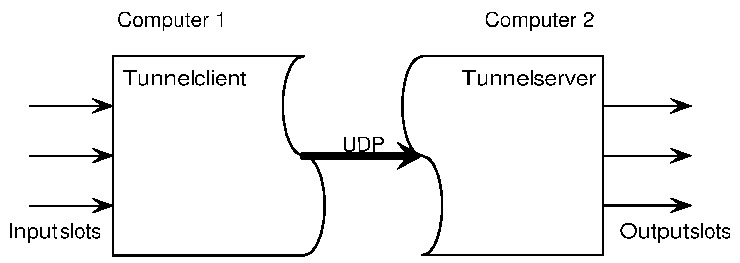
\includegraphics[width=8cm]{pics/tunnel}
%\caption{Tunnel component}
%\label{tunnel_pic}
\end{center}
%\end{figure}

An instance of the tunnel component either represents the input part
(client) or the output part (server). Value changes on the client are
then propagated via UDP datagrams to the server. When creating either
side of the tunnel you have to define the name and type of the slots
that should be created. The slot types of the client and the server
should always match.

\note{ArraySlots are currently not supported.}

\begin{classdesc}{Tunnel}{name = "Tunnel",\\ 
			  server = False, \\
                          slots = None, \\
                          port = 64738, \\
                          host = "localhost", \\
			  gather_messages = False, \\
                          verbose = False, \\
                          auto_insert = True}

\var{server} determines which end of the tunnel is created. The server is
always the ``end'' of a tunnel, i.e. where the values leave the
tunnel.  

\var{slots} specifies the slots to create on the tunnel. It
must be a list of 2-tuples containing two strings. The first string is
the name of the attribute and the second contains the type and
initializer of the slot (in Python syntax). The order and types of the
slots on the client and server should always match.  

\var{port} is the port number to use for the data transfer. The server
listens on this port and the client sends its data to this port on the
target machine.

\var{host} is a string containing the name or IP address of the target
machine where the server part of the tunnel is located. This parameter
is only used on the client side.

\var{gather_messages} determines whether value change messages should be
gathered and sent as one single message or not. If this flag is \code{False},
a message will be sent to the server whenever the value of a slot changes.
However, sometimes it may be the case that you can guarantee that all slots
will change their value at the same time. In such cases, you can set 
\var{gather_messages} to \code{True} which will have the effect that all
messages are collected and delayed until the {\em last} slot receives its 
new value. Only then will the value changes be sent as one big message
which increases the network performance.

If you set \var{verbose} to \code{True} the component will print some
messages so you can follow what it is doing.

\end{classdesc}


Here is an example of a sphere whose position is controlled by a remote
machine:

\begin{verbatim}
# Server code (machine A):

# Create a sphere...
s = Sphere()

# ...and the end of a tunnel that has one Vec3Slot called "pos"
t = Tunnel(
    server = True,
    slots = [("pos", "Vec3Slot()")]
)

# Connect the tunnel slot with the position of the sphere
t.pos_slot.connect(s.pos_slot)
\end{verbatim}

Execute this script with the viewer tool on machine A:

\begin{verbatim}
viewer.py server.py
\end{verbatim}

On the remote machine (the client) you can set the position of the above
sphere with the following code:

\begin{verbatim}
# Client code (machine B):

from cgkit import *

# Create the "entrance" of the tunnel...
t = Tunnel(
    slots = [("pos", "Vec3Slot()")],
    host = "<name or IP of machine A>"
)

# Move the sphere to position (1,0,0)
t.pos_slot.setValue(vec3(1,0,0))
\end{verbatim}

You can call this script by invoking it directly on machine B:

\begin{verbatim}
python client.py
\end{verbatim}

Calling the client code will move the sphere in the first program to 
the position (1,0,0). 

\begin{notice}[note]
As the underlying transport mechanism is using UDP datagrams there is no
error reporting mechanism. The client has no chance of knowing whether
a value change was properly propagated to the server or not. So if you
encounter any problems such as the sphere in the above example {\em not}
moving to another position, you can set the \var{verbose} flag to \code{True}
and additionally check the following points:

\begin{itemize}
\item Do the port numbers on the client and server match?
\item Did you specify the correct host name (or IP address) on the client side?
\item Is there a firewall blocking the network traffic?
\item Did you set \var{gather_messages} to \code{True} and the last slot 
  does not receive any new values? (try to set \var{gather_messages} to
  \code{False})
\end{itemize}

\end{notice}

% ODEDynamics component

\section{\class{ODEDynamics} ---
         Rigid body dynamics using the Open Dynamics Engine}

\begin{classdesc}{ODEDynamics}{name = "ODEDynamics",\\ 
			       gravity = 9.81, \\
                               substeps = 1, \\
                               enabled = True, \\
                               erp = None, \\
                               cfm = None, \\
                               defaultcontactproperties = None, \\
                               collision_events = False, \\
                               auto_add = False, \\
                               show_contacts = False, \\
                               contactmarkersize = 0.1, \\
                               contactnormalsize = 1.0, \\
                               auto_insert = True}

\var{gravity} is the acceleration due to gravity. The direction of the
acceleration is in negative "up" direction (as specified by the scene).

\var{substeps} is the number of simulation steps per frame. You can
increase this value to get a more accurate/stable simulation.

The simulation will only run if \var{enabled} is \code{True}, otherwise
it's halted.

\var{erp} and \var{cfm} are the global error reduction parameter and
constraint force mixing value to be useed (see the ODE manual).

\var{defaultcontactproperties} is a \class{ODEContactProperties} object
that specifies the default contact parameters. These parameters are
used for contacts between two objects (resp. materials) that have not
been set explicitly using \method{setContactProperties()}.

\var{collision_events} determines whether the component will generate
\code{ODE_COLLISION} events whenever a collision has occured. An event
handler takes a \class{ODECollisionEvent} (see section 
\ref{odecollisionevent}) object as argument.

If \var{auto_add} is \code{True} the component searches the scene for
rigid bodies and hinges and adds them automatically to the component.
This is done at the time the component is created, so any bodies or
hinges created afterwards will be ignored.

\var{show_contacts} determines whether the contact points and normals
are visualized or not (this is mainly for debugging purposes).
The size of the contact point markers and the length of the normals
can be specified via the \var{contactmarkersize} and \var{contactnormalsize}
arguments.
\end{classdesc}

\begin{methoddesc}{add}{objects, categorybits=None, collidebits=None}
Add world objects to the simulation. \var{objects} can be a single
object or a sequence of objects. An object may be specified by its
name or the object itself. \var{categorybits} and \var{collidebits}
are long values that control which objects can collide with which
other object. The specified category and collide bits are assigned to every
object in \var{objects}. Each bit in \var{categorybits} represents
one category the objects belong to. \var{collidebits} is another bit
field that specifies with which categories the objects may collide.
By default, every bit is set in both values.
\end{methoddesc}

\begin{methoddesc}{reset}{}
Reset the state of the simulated bodies. All bodies will be set to the
position and velocity they had when they were added to the simulation.
This method is also called when the RESET event is issued.
\end{methoddesc}

\begin{methoddesc}{setContactProperties}{(mat1, mat2), props}
Set the contact properties for a material pair. \var{mat1} and \var{mat2}
are two \class{Material} objects and props is a \class{ODEContactProperties}
object describing the contact properties.
\end{methoddesc}

\begin{methoddesc}{getContactProperties}{(mat1, mat2)}
Return the contact properties for a material pair. The order of the materials
is irrelevant. The return value is
a \class{ODEContactProperties} object. A default property object is
returned if the pair does not have any properties set.
\end{methoddesc}

\begin{methoddesc}{createBodyManipulator}{object}
Return an \class{ODEBodyManipulator} object that can be used to apply
external forces/torques to the world object \var{object}.
\end{methoddesc}


\begin{notice}[note]
To use the \class{ODEDynamics} component the
\ulink{PyODE}{http://pyode.sourceforge.net/} module has to be 
installed on your system which wraps the 
\ulink{Open Dynamics Engine}{http://www.ode.org/}.
\end{notice}

%------------------------------------------------------
\subsection{\class{ODEContactProperties} ---
         Contact properties during collision}

The \class{ODEContactProperties} class contains all the parameters
that are used when two objects collide. 

\begin{classdesc}{ODEContactProperties}{mode = 0,\\
			       mu = 0.3,\\
			       mu2 = None,\\
			       bounce = None,\\
			       bounce_vel = None,\\
			       soft_erp = None,\\
			       soft_cfm = None,\\
			       motion1 = None,\\
			       motion2 = None,\\
			       slip1 = None,\\
			       slip2 = None,\\
			       fdir1 = None}

See the ODE manual (chapter 
\ulink{7.3.7 {\em Contact}}{http://ode.org/ode-latest-userguide.html#sec_7_3_7})
for an explanation of these
parameters.

\note{You only have to specify the \var{mode} argument if you want to set
the ContactApprox* flags. The other flags are automatically set.}
\end{classdesc}

%------------------------------------------------------
\subsection{\class{ODEBodyManipulator} ---
         Apply external forces/torques to bodies}

The \class{ODEBodyManipulator} class can be used to apply external
forces and torques to a rigid body. 

\begin{classdesc*}{ODEBodyManipulator}
You get an instance of this class
by calling the
\method{createBodyManipulator()} method of the \class{ODEDynamics} component.
One particular body manipulator instance is always associated with one
particular rigid body. A manipulator object has the following attributes
and methods:
\end{classdesc*}

\begin{memberdesc}{body}
This attribute contains the rigid body (\class{WorldObject}) this
manipulator is associated with. You can only read this attribute. If
you want to control another body, use the
\method{createBodyManipulator()} method of the dynamics component.
\end{memberdesc}

\begin{memberdesc}{odebody}
This is the Body instance of the PyODE module. You can use this object
if you want to access special features of ODE that are not exposed otherwise.
But note that you won't get the expected results if you call methods like
\method{addForce()} directly on the ODE body and you're using more than
one sub step in your simulation. The force would only be applied during
the first sub step because it is reset after each step. Use this
manipulator class instead, that's what it's for.
\end{memberdesc}

% addForce
\begin{methoddesc}{addForce}{force, relforce=False, pos=None, relpos=False}
Add an external force to the current force vector. \var{force} is a vector
containing the force to apply. If \var{relforce} is \code{True} the force
is interpreted in local object space, otherwise it is assumed to be given
in global world space. By default, the force is applied at the center
of gravity. You can also pass a different position in the \var{pos} argument
which must describe a point in space. \var{relpos} determines if the
point is given in object space or world space (default).
\end{methoddesc}

% addTorque
\begin{methoddesc}{addTorque}{torque, reltorque=False}
Add an external torque to the current torque vector. \var{torque} is
a vector containing the torque to apply. \var{reltorque} determines if
the torque vector is given in object space or world space (default).
\end{methoddesc}

% setInitialPos
\begin{methoddesc}{setInitialPos}{pos}
Set the initial position of the body. \var{pos} must be a 3-sequence of 
floats containing the new position.
\end{methoddesc}

% setInitialRot
\begin{methoddesc}{setInitialRot}{rot}
Set the initial orientation of the body. \var{rot} must be a
\class{mat3} containing a rotation matrix.
\end{methoddesc}

% setInitialLinearVel
\begin{methoddesc}{setLinearVel}{vel}
Set the initial linear velocity of the body. \var{vel} must be a
3-sequence of floats containing the new velocity.
\end{methoddesc}

% setInitialAngularVel
\begin{methoddesc}{setAngularVel}{vel}
Set the initial angular velocity of the body. \var{vel} must be a
3-sequence of floats containing the new velocity.
\end{methoddesc}

% setPos
\begin{methoddesc}{setPos}{pos}
Set the position of the body. \var{pos} must be a 3-sequence of floats
containing the new position.
\end{methoddesc}

% setRot
\begin{methoddesc}{setRot}{rot}
Set the orientation of the body. \var{rot} must be a \class{mat3} containing a
rotation matrix.
\end{methoddesc}

% setLinearVel
\begin{methoddesc}{setLinearVel}{vel}
Set the linear velocity of the body. \var{vel} must be a 3-sequence of floats
containing the new velocity.
\end{methoddesc}

% setAngularVel
\begin{methoddesc}{setAngularVel}{vel}
Set the angular velocity of the body. \var{vel} must be a 3-sequence of floats
containing the new velocity.
\end{methoddesc}

%------------------------------------------------------
\subsection{\class{ODECollisionEvent} ---
         Collision event object}
\label{odecollisionevent}

An \class{ODECollisionEvent} object is passed as argument to the event
handler for \code{ODE_COLLISION} events.

\begin{classdesc}{ODECollisionEvent}{obj1, obj2, contacts, contactproperties}

\var{obj1} and \var{obj2} are the two world objects that have collided with 
each other.

\var{contacts} is a list of \class{ode.Contact} objects that each describes
a contact point.

\var{contactproperties} is a \class{ODEContactProperties} object that
describes the properties of the contact. It depends on the materials
of the \var{obj1} and \var{obj2}. The event handler may modify
this object to change the result of the collision. Note however, that
the changes will be permanent and also affect later collisions.
\end{classdesc}

% averageContactGeom
\begin{methoddesc}{averageContactGeom}{}
Return the average contact position, normal and penetration depth (in
this order). The position and normal are returned as \class{vec3}
objects, the penetration depth is a float.
\end{methoddesc}

% FlockOfBirds component

\section{\class{FlockOfBirds} ---
         Retrieving values from an Ascension Flock of Birds\textsuperscript{\textregistered} motion tracker}

The \class{FlockOfBirds} class communicates with an Ascension Flock
of Birds\textsuperscript{\textregistered} motion tracker 
(\url{http://www.ascension-tech.com/}) via the serial port and provides the 
sensor values of the individual birds via slots.

Note: Currently, the class assumes that an extended range controller is
used! (this means the position values have to be adjusted if you use the
tracker without an extended range controller)

\begin{classdesc}{FlockOfBirds}{name = "FlockOfBirds",\\ 
                                com_port = 0,\\
                                baud_rate = 115200,\\
                                timeout = 2.0,\\
                                num_birds = 1,\\
                                bird_mode = "p",\\
                                hemisphere = "forward",\\
                                auto_insert = True}


\var{com_port} specifies which COM port to use for the communication with
the flock (0-based port number).

\var{baud_rate} is the baud rate to use.

\var{timeout} specifies a time span in seconds after which a RS232 operation
fails.

\var{num_birds} is the number of birds to use (including the ERC which will 
be bird 1).

\var{bird_mode} selects what kind of data the birds will send. It can be either
a string containing the mode for all birds or it can be a list of strings
to select a mode for each individual bird. In the latter case, the list must
hold one string for each bird. The mode string can be one of the values
in the following table:

\begin{tableii}{c|l}{code}{Mode}{Description}
\lineii{"p"}{Send only the position.}
\lineii{"a"}{Send only euler angles.}
\lineii{"m"}{Send only a rotation matrix.}
\lineii{"q"}{Send only a quaternion.}
\lineii{"pa"}{Send position and euler angles.}
\lineii{"pm"}{Send position and matrix.}
\lineii{"pq"}{Send position and quaternion.}
\end{tableii}

\var{hemisphere} specifies in which hemisphere, centered about the
transmitter, the sensor will be operating (see the {\em Flock of Birds ---
Installation and Operation Guide}). The values can be one of \code{"forward"},
\code{"aft"}, \code{"upper"}, \code{"lower"}, \code{"left"} and \code{"right"}.

\end{classdesc}


For each bird, the \class{FlockOfBirds} component creates the following
four slots:

\begin{itemize}
\item \code{pos<n>_slot} (\code{Vec3Slot}) -- Position (in cm)
\item \code{angle<n>_slot} (\code{Vec3Slot}) -- Euler angles
\item \code{matrix<n>_slot} (\code{Mat3Slot}) -- Rotation matrix
\item \code{quat<n>_slot} (\code{QuatSlot}) -- Quaternion
\end{itemize}

where \code{<n>} is the number of the bird (1-based). Not all of the
slots are active at the same time. You can select which slot should
carry the corresponding value via the bird mode.

\begin{notice}[note]
To use the \class{FlockOfBirds} component the
\ulink{pySerial}{http://pyserial.sourceforge.net/} module has to be 
installed on your system.
\end{notice}


% GnuPlotter component

\section{\class{GnuPlotter} ---
         Plot values using Gnuplot}

The \class{GnuPlotter} class can be used to plot the graph of a
floating point slot. To do so, connect any \class{DoubleSlot} to
an input slot of the plotter. The input slots are called \code{input<n>_slot}
where \code{<n>} is the number of the slot.

\begin{classdesc}{GnuPlotter}{name = "GnuPlotter",\\ 
                              title = None, \\
                              xlabel = None, \\
                              ylabel = None, \\
                              xrange = None, \\
                              yrange = None, \\
                              inputs = 1, \\
                              plottitles = [], \\
                              starttime = 0.0, \\
                              endtime = 99999.0, \\
                              enabled = True, \\
                              auto_insert = True}

\var{title} is a string containing the title of the entire plot.

\var{xlabel}, \var{ylabel} are strings containing the labels for the X and
Y axis.

\var{xrange}, \var{yrange} is each a 2-tuple (\var{start}, \var{end}) 
containing the range of the X axis resp. Y axis.

\var{inputs} is the number of input slots that should be created (i.e.
the number of curves you want to plot).

\var{plottitles} is a list of strings containing the name of the respective
curve.

\var{starttime} and \var{endtime} defines the range in which values are
received and plotted. The times are given in seconds.

\var{enabled} is a flag that can be used to disable the plotter.
\end{classdesc}

A \class{GnuPlotter} object has the following slots:

\begin{tableiv}{l|l|c|l}{code}{Slot}{Type}{Access}{Description}
\lineiv{input1_slot}{float}{rw}{First curve}
\lineiv{input2_slot}{float}{rw}{Second curve}
\lineiv{...}{...}{...}{...}
\end{tableiv}

% --------------------
\begin{notice}[note]
To use the \class{GnuPlotter} component the
\ulink{Gnuplot.py}{http://gnuplot-py.sourceforge.net/} module has to be 
installed on your system (and of course, 
\ulink{gnuplot}{http://www.gnuplot.info/} itself as well).
\end{notice}


% PIDController component

\section{\class{PIDController} ---
         Proportional-Integral-Derivative controller}

A PID controller is a standard component in industrial control
applications which tries to keep a measured value at a given target
value (the {\em setpoint}). The measured value has to be plugged into
the input slot (\code{input_slot}) and the output of the PID controller
can be read from \code{output_slot}.

%\begin{displaymath}
%output(t) = K_p \cdot err(t) + K_i \cdot \int err(t')\, dt' + K_d \cdot \frac{d\,err}{dt}
%\end{displaymath}

For example, you can use a PID controller in conjunction with the
joints in the \class{ODEDynamics} component to keep a hinge or slider
at a particular position. In this case the angle or position is used
as input to the PID controller and the output controls the motor velocity.

\begin{classdesc}{PIDController}{name = "PIDController",\\ 
                              setpoint = 0.0, \\
                              Kp = 0.0, \\
                              Ki = 0.0, \\
                              Kd = 0.0, \\
                              maxout = 999999, \\
                              minout = -999999, \\
                              auto_insert = True}

\var{setpoint} is the target value that should be maintained.

\var{Kp} is the weight for the proportional part, \var{Ki} the weight
for the integral part and \var{Kd} the weight for the derivative part.

\var{maxout} and \var{minout} are used to clamp the output value.
\end{classdesc}

A \class{PIDController} has the following slots:

\begin{tableiv}{l|l|c|l}{code}{Slot}{Type}{Access}{Description}
\lineiv{input_slot}{float}{rw}{The "measured" value}
\lineiv{setpoint_slot}{float}{rw}{The target value}
\lineiv{output_slot}{float}{r}{Controller output}
\lineiv{maxout_slot}{float}{rw}{Maximum output value}
\lineiv{minout_slot}{float}{rw}{Minimum output value}
\lineiv{Kp_slot}{float}{rw}{Weight for the proportional term}
\lineiv{Ki_slot}{float}{rw}{Weight for the integral term}
\lineiv{Kd_slot}{float}{rw}{Weight for the derivative term}
\end{tableiv}




% SlideShow component

\section{\class{SlideShow} ---
         Displaying a series of images}

The \class{SlideShow} class can be used to display image files as
a slide show. The component sets up a scene and displays an image
sequence with user defined transitions.

\begin{classdesc}{SlideShow}{name = "SlideShow",\\ 
                             slides = [], \\
                             auto_insert = True}

\var{slides} is either a string specifying the image files (the string
may contain wildcards) or a list of \class{Slide} objects where each
object represents one or more images.
\end{classdesc}

Example:

\begin{verbatim}
# File: slides.py

SlideShow(
    slides = [
              Slide("image01.jpg", XFade(1.0) ),
              Slide("image02.jpg", XFade(1.0, 0.3) ),
              Slide("image03.jpg", XCube(2.0) ),
              Slide("presentation/slides*.png", XFade(0.5) )
             ]
)
\end{verbatim}

The slide show is started with the viewer tool like this:

\begin{verbatim}
viewer.py slides.py -f50 -F
\end{verbatim}

In this case, the frame rate is increased to 50 frames per second (to get
smoother transitions) and the display is set to full screen.

When the slide show is running you can jump to the next slide by pressing
a mouse button, the \kbd{Enter} key or the \kbd{PageDown} key.
In case you move the camera, you can reset it with the \kbd{q} key.

%----------------------------------------------------------------------
\subsection{Slide class}

The \class{Slide} class represents one or more image files and contains
one transition that is used for all files.

\begin{classdesc}{Slide}{filepattern, transition = XCube()}

\var{filepattern} specifies the image files to load and may include
wildcards to select more than one file.

\var{transition} is a transition class that determines the transition
that is applied after each image in this slide object.
\end{classdesc}

%----------------------------------------------------------------------
\subsection{XFade transition}

The \class{XFade} transition implements a smooth cross fade between two
images.

\begin{classdesc}{XFade}{duration=2.0, zmove=0.0}

\var{duration} is the length of the transition in seconds.

If \var{zmove} is greater than 0, the old image will be moved towards
the camera during the transition which makes it scale up when viewed
with a perspective camera.
\end{classdesc}

%----------------------------------------------------------------------
\subsection{XCube transition}

The \class{XCube} class implements a transition where the images seem
to be attached on two adjacent sides of a cube and the cube rotates
during the transition.

\begin{classdesc}{XCube}{duration=2.0}

\var{duration} is the length of the transition in seconds.
\end{classdesc}


% MotionPath

\section{\class{MotionPath} ---
         Motion path}

\begin{classdesc}{MotionPath}{name = "MotionPath",\\ 
                              curve = None,\\
                              begintime = 0.0,\\
                              endtime = 1.0,\\
                              loop = False,\\
                              follow = False,\\
                              bank = False,\\
                              bankamplitude = 0.1,\\
                             }

\var{curve} is an object supporting the curve protocol.

\var{begintime} and \var{endtime} specify the parameter interval of
the motion. At \var{begintime} the object will be located at the beginning
of the curve and at \var{endtime} it will be at the end.

\var{loop} is a boolean that specifies if the motion is repeated when 
outside the specified parameter interval.

\var{follow} determines if the object will change its orientation to
follow the path.

\var{bank} determines if the object will roll if the curve makes a turn.
\var{bankamplitude} specifies how much the obect will roll.

\end{classdesc}




%---
\chapter{WorldObjects \label{worldobjects}}

% WorldObject

\section{\class{WorldObject} ---
         World object base class}

\begin{classdesc}{WorldObject}{name = "object", \\
                 transform = None,\\
                 pos = None, \\
	         rot = None,\\
                 scale = None,\\
                 pivot = None,\\
                 offsetTransform = None,\\
                 parent = None,\\
                 mass = None,\\
                 material = None,\\
                 visible = True,\\
                 auto_insert = True}

\var{name} is the name of the object which can be used to identify the
object.

\var{transform} is the initial transformation that should be applied to
the object. Alternatively, you can specify the individual components
\var{pos}, \var{rot} and \var{scale}.

\var{pivot} is the pivot point of the object. This is the 4th column of
the offset transformation. You can also specify the entire offset 
transformation using the \var{offsetTransform} argument.

\var{parent} is the parent world object and determines at which position
in the scene graph the new object is added. If \var{parent} is \code{None}
the object will become a child of the world root. The \var{parent} argument
is only used if \var{auto_insert} is \code{True}.

\var{mass} is the mass of this object (this does {\em not} include
the children objects).

\var{material} describes the appearance of the object. It can be either 
a single \class{Material} object or a sequence of \class{Material} objects.

\var{visible} is a flag that determines whether the object is visible
or not. This only affects the geometry of this WorldObject, it is not
inherited by children objects.

The object will be inserted into the scene automatically if 
\var{auto_insert} is set to \code{True}.
\end{classdesc}

A \class{WorldObject} always has the following slots:

\begin{tableiv}{l|l|c|l}{code}{Slot}{Type}{Access}{Description}
\lineiv{angularvel_slot}{vec3}{rw}{Angular velocity}
\lineiv{cog_slot}{vec3}{r}{Center of gravity}
\lineiv{inertiatensor_slot}{mat3}{r}{Inertia tensor}
\lineiv{linearvel_slot}{vec3}{rw}{Linear velocity}
\lineiv{mass_slot}{float}{rw}{Mass of the local geometry}
\lineiv{pos_slot}{vec3}{rw}{Position}
\lineiv{rot_slot}{mat3}{rw}{Orientation}
\lineiv{scale_slot}{vec3}{rw}{Scaling}
\lineiv{totalmass_slot}{float}{r}{Total mass (including the children)}
\lineiv{transform_slot}{mat4}{rw}{Object transformation}
\lineiv{visible_slot}{bool}{rw}{Visibility flag}
\lineiv{worldtransform_slot}{mat4}{rw}{World transformation}
\end{tableiv}

\begin{memberdesc}{geom}
This attribute holds the visible geometry which must be derived from 
\class{GeomObject}. The value can also be \code{None} if there is no
visible geometry. Geometry objects can be shared between different 
world objects. This value can be read and written.
\end{memberdesc}

\begin{memberdesc}{parent}
This attribute contains the parent world object or \code{None}. You can 
only read this attribute.
\end{memberdesc}

\begin{memberdesc}{transform}
This is the value of the mat4 slot \var{transform_slot} which contains
the object transformation T. You can read and write this attribute.
\end{memberdesc}

\begin{memberdesc}{worldtransform}
This is the value of the mat4 slot \var{worldtransform_slot} which
contains the world transformation (which is a concatenation of all local
transformations L). You can only read this attribute.

\note{Note that in contrast to the \var{transform} slot,
the \var{worldtransform} is not influenced by the offset transformation.}
\end{memberdesc}

\begin{memberdesc}{pos}
This is the value of the vec3 slot \var{pos_slot} which contains the 
position of the object. You can read and write this attribute.
\end{memberdesc}

\begin{memberdesc}{rot}
This is the value of the mat3 slot \var{rot_slot} which contains the 
orientation of the object. You can read and write this attribute.
\end{memberdesc}

\begin{memberdesc}{scale}
This is the value of the vec3 slot \var{scale_slot} which contains the 
scaling of the object. You can read and write this attribute.
\end{memberdesc}

\begin{memberdesc}{pivot}
This is the pivot point (vec3) of the object. You can read and write this
attribute. Reading or writing this attribute is equivalent to calling
\method{getOffsetTransform()} or \method{setOffsetTransform()} with
a matrix that only modifies the 4th column.
\end{memberdesc}

\begin{memberdesc}{cog}
This is the value of the vec3 slot \var{cog_slot} which contains the
physical center of gravity. This value is derived from the center of 
gravity provided by the geometry object and the cogs and masses of the
children objects. This means it represents the center of gravity of the 
entire hierarchy. The value is given with respect to the pivot coordinate
system P. You can only read this value.
\end{memberdesc}

\begin{memberdesc}{inertiatensor}
This is the value of the mat3 slot \var{inertiatensor_slot} which contains
the inertia tensor of the entire hierarchy (just like \var{cog}). You can
only read this value.
\end{memberdesc}

\begin{memberdesc}{mass}
This is the value of the double slot \var{mass_slot} which contains the
{\em local} mass of this object (not including the children). Or in other
words, this is the mass of the geometry directly set in this object.
You can read and write this value.
\end{memberdesc}

\begin{memberdesc}{totalmass}
This is the value of the double slot \var{totalmass_slot} which contains
the total mass of this object and its children. You can only read this value.
\end{memberdesc}

\begin{memberdesc}{angularvel}
This is the value of the vec3 slot \var{angular_slot} which contains the 
angular velocity of the object. The value is not computed but has to be
set by anyone who knows the angular velocity (such as a dynamics component).
You can read and write this attribute.
\end{memberdesc}

\begin{memberdesc}{linearvel}
This is the value of the vec3 slot \var{linearvel_slot} which contains the 
linear velocity of the object. The value is not computed but has to be
set by anyone who knows the linear velocity (such as a dynamics component).
You can read and write this attribute.
\end{memberdesc}


% Methods
\begin{methoddesc}{boundingBox}{}
Return the local axis aligned bounding box. The bounding box is
given with respect to the local transformation L (which is not
what you get from the transform slot of the world object).
\end{methoddesc}

\begin{methoddesc}{localTransform}{}
Returns the local transformation that has to be used for rendering.
The returned transformation L is calculated as follows: $L = T\cdot P^{-1}$,
where T is the current transform (taken from the transform slot)
and P is the offset transform.
\end{methoddesc}

\begin{methoddesc}{getOffsetTransform}{}
Return the current offset transformation as a \class{mat4}. This
transformation is given relative to the local object transformation.
\end{methoddesc}

\begin{methoddesc}{setOffsetTransform}{P}
Set the offset transformation. The transformation has to be given
relative to the local object transformation. After setting the offset
transformation, the transform slot will be updated so that 
\method{localTransform()} returns the same matrix as before, i.e. the
world position/orientation of the object does not change.
\end{methoddesc}

\begin{methoddesc}{getNumMaterials}{}
Return the current size of the material array.
\end{methoddesc}

\begin{methoddesc}{setNumMaterials}{num}
Set a new size for the material array.
\end{methoddesc}

\begin{methoddesc}{getMaterial}{idx=0}
Get a stored material. The method returns \code{None} if the given index
is out of range or there is no material stored at that position.
\end{methoddesc}

\begin{methoddesc}{setMaterial}{mat, idx=0}
Set a new material. An \exception{IndexError} exception is thrown if
the index is out of range.
\end{methoddesc}

\begin{methoddesc}{lenChilds}{}
Return the number of children objects.
\end{methoddesc}

\begin{methoddesc}{iterChilds}{}
Return an iterator that iterates over all children objects.
\end{methoddesc}

\begin{methoddesc}{hasChild}{name}
Check if a children with a particular name does exist.
\end{methoddesc}

\begin{methoddesc}{child}{name}
Return the children with a particluar name. A \exception{KeyError}
exception is thrown if there is no children with the specified name.
\end{methoddesc}

\begin{methoddesc}{addChild}{child}
Add a new children world object to this object. A
\exception{ValueError} exception is thrown if child was already added
to another object.  In this case you have to remove the object from
its previous parent yourself. You also have to make sure that the name
of \var{child} is unique among the children of this object, otherwise
a \exception{KeyError} exception is thrown.
\end{methoddesc}

\begin{methoddesc}{removeChild}{child}
Remove a children world object from this object. \var{child} can either
be the name of the children or the object itself. A \exception{KeyError}
exception is thrown if child is not a children of this object.
\end{methoddesc}

\begin{methoddesc}{makeChildNameUnique}{name}
Modify \var{name} so that it is unique among the children names. If
\var{name} is already the name of a children object, then it is modified
by adding/increasing a trailing number, otherwise it is returned
unchanged.
\end{methoddesc}





% Box

\section{\class{Box} ---
         Box object}

\begin{classdesc}{Box}{name = "Box",\\ 
                       lx = 1.0,\\
                       ly = 1.0,\\
                       lz = 1.0,\\
                       segmentsx = 1,\\
                       segmentsy = 1,\\
                       segmentsz = 1,\\
%                       transform = None,\\
%                       pos = None,\\
%                       rot = None,\\
%                       scale = None,\\
%                       pivot = None,\\
%                       offsetTransform = None,\\
%                       material = None,\\
%                       mass = None,\\
                       dynamics = True,\\
                       static = False,\\
                       ...[WorldObject params]...
                       }

\end{classdesc}



% Sphere

\section{\class{Sphere} ---
         Sphere object}

\begin{classdesc}{Sphere}{name = "Sphere",\\ 
                       radius = 1.0,\\
                       segmentsu = 16,\\
                       segmentsv = 8,\\
%                       transform = None,\\
%                       pos = None,\\
%                       rot = None,\\
%                       scale = None,\\
%                       pivot = None,\\
%                       offsetTransform = None,\\
%                       material = None,\\
%                       mass = None,\\
                       dynamics = True,\\
                       static = False,\\
%                       auto_insert = True\\
                       ...[WorldObject params]...
		       }

\end{classdesc}



% Capped Cylinder

\section{\class{CCylinder} ---
         Capped cylinder object}

\begin{classdesc}{CCylinder}{name = ''CCylinder'',\\ 
                       radius = 1.0,\\
                       length = 1.0,\\
                       segmentsu = 16,\\
                       segmentsvl = 1,\\
                       segmentsvr = 4,\\
%                       transform = None,\\
%                       pos = None,\\
%                       rot = None,\\
%                       scale = None,\\
%                       pivot = None,\\
%                       offsetTransform = None,\\
%                       material = None,\\
%                       mass = None,\\
                       dynamics = True,\\
                       static = False,\\
                       ...[WorldObject params]...
                       }

\end{classdesc}



% Plane

\section{\class{Plane} ---
         Plane object}

\begin{classdesc}{Plane}{name = ''Plane'',\\ 
                       lx = 1.0,\\
                       ly = 1.0,\\
                       segmentsx = 1,\\
                       segmentsy = 1,\\
                       transform = None,\\
                       pos = None,\\
                       rot = None,\\
                       scale = None,\\
                       pivot = None,\\
                       offsetTransform = None,\\
                       material = None,\\
                       mass = None,\\
                       dynamics = True,\\
                       auto_insert = True}

\end{classdesc}



% Torus

\section{\class{Torus} ---
         Torus object}

\begin{classdesc}{Torus}{name = "Torus",\\ 
                         major = 1.0,\\
                         minor = 0.1,\\
                         segmentsu = 16,\\
                         segmentsv = 8,\\
                         ...[WorldObject params]...
	   	       }

\end{classdesc}



% TriMesh

\section{\class{TriMesh} ---
         Triangle mesh object}

\begin{classdesc}{TriMesh}{name = ''TriMesh'',\\ 
                       verts = [],\\
                       faces = [],\\
                       transform = None,\\
                       pos = None,\\
                       rot = None,\\
                       scale = None,\\
                       pivot = None,\\
                       offsetTransform = None,\\
                       material = None,\\
                       mass = None,\\
                       dynamics = True,\\
                       static = False,\\
                       auto_insert = True}

\end{classdesc}



% Polyhedron

\section{\class{Polyhedron} ---
         Polyhedron object}

\begin{classdesc}{Polyhedron}{name = "Polyhedron",\\ 
                              verts = [],\\
                              polys = []
			     }	

\end{classdesc}



% Group

\section{\class{Group} ---
         Group object}

\begin{classdesc}{Group}{name = ''Group'',\\ 
                       childs = [],\\
                       transform = None,\\
                       pos = None,\\
                       rot = None,\\
                       scale = None,\\
                       pivot = None,\\
                       offsetTransform = None,\\
                       dynamics = True,\\
                       static = False,\\
                       auto_insert = True}

\end{classdesc}



% Joint

\section{\class{Joint} ---
         Joint class for creating a skeleton}

The \class{Joint} class can be used to create articulated
characters. Bones are implicitely created by linking two joints, i.e.
a bone is assumed between a joint and each of its children joints.
A \class{Joint} object corresponds to a ball joint that has three rotational
degrees of freedom. The actual joint is always located at the pivot point
of the \class{Joint} object and rotates about the pivot frame axes.

If you want your local coordinate frame to be oriented differently, it
is not enough to set the offset transform as this will also readjust the
local frame so that the effect is actually cancelled out and you will
still rotate about the same axes as before. To initialize the new frame
you have to call \method{freezePivot()} after setting the offset transform.
This will set the current offset transform as the new default pose where
all angles are 0 and will make the joint rotate about the new axes.
After freezing you may want to set the offset transform back to the identity
so that the local coordinate frame and the offset frame coincide again.
This won't affect the rotation of the joint but the location of its
children (as setting the offset transform on a \var{Joint} object also
modifies its local coordinate system). But it actually depends on the
situation whether you have to reset the offset transform or not.

Rotating a joint is not done by setting its \var{rot} attribute but
by setting its three individual angles (\var{anglex}, \var{angley}, 
\var{anglez}).

\begin{classdesc}{Joint}{name = "", \\
			 radius = 0.05, \\
	                 rotationorder = "xyz"
		         }

\var{name} is the name of the joint.

\var{radius} is the radius of the visual representation of the joint/bone.

\var{rotationorder} determines the order of rotation about the individual
axes.
\end{classdesc}

A \class{Joint} has the following slots:

\begin{tableiv}{l|l|c|l}{code}{Slot}{Type}{Access}{Description}
\lineiv{anglex_slot}{float}{rw}{Angle around x axis}
\lineiv{angley_slot}{float}{rw}{Angle around y axis}
\lineiv{anglez_slot}{float}{rw}{Angle around z axis}
\end{tableiv}

\begin{memberdesc}{anglex}
Rotation angle (in degrees) about the local x axis.
\end{memberdesc}

\begin{memberdesc}{angley}
Rotation angle (in degrees) about the local y axis.
\end{memberdesc}

\begin{memberdesc}{anglez}
Rotation angle (in degrees) about the local z axis.
\end{memberdesc}

% Methods
\begin{methoddesc}{freezePivot}{}
Make the current pivot coordinate system the default pose. After
calling this method, the current rotation of the pivot coordinate
system will define the default pose. This means, rotations are now
defined around the local pivot axes. 
\end{methoddesc}







% TargetCamera

\section{\class{TargetCamera} ---
         Target camera}

The \class{TargetCamera} class always looks at a specified point and
aligns its local up direction to the scene up direction.

\begin{classdesc}{TargetCamera}{name = "TargetCamera",\\ 
                       target = (0,0,0),\\
                       fov = 45.0,\\
                       roll = 0.0, \\
                       up = None,\\
                       focallength = 0,\\
                       fstop = 0,\\
                       auto_nearfar = True,\\
                       nearplane = 0.1,\\
                       farplane = 1000.0,\\
                       }

\var{target} is the point that the camera will always look at. 

\var{fov} is the field of view in degrees (in vertical direction), i.e.
the angle between the bottom and the top of the screen.

\var{roll} is an angle in degrees that the camera is rotated about its 
local z axis.

\var{up} is the vector that is considered to be the 'up' direction. If
\code{None} is passed, the global 'up' direction from the scene is used.

\var{focallength} is the focal length of the camera and \var{fstop} the
aperture number that determines the lens diameter. These values are used
to turn on depth of field. Depth of field is activated if both attributes
are set to a value different from 0 (note however, that not every renderer
supports depth of field). The focal distance is set so that the target 
point will always be in focus.

\var{auto_nearfar} specifies whether the near and far plane
distances are automatically determined or if fixed values are used.
If set to \code{False}, the \var{nearplane} and \var{farplane} arguments
are used, otherwise the values are computed from the objects in the scene.
In the latter case, the \var{nearplane} value still serves as minimum
value for the near plane distance which is used when the camera is located
within the scene bounds.
\end{classdesc}

The \class{TargetCamera} has the following slots (in addition to the slots
of the \class{WorldObject} base class):

\begin{tableiv}{l|l|c|l}{code}{Slot}{Type}{Access}{Description}
\lineiv{target_slot}{vec3}{rw}{Target point}
\lineiv{fov_slot}{float}{rw}{Field of view in degrees}
\lineiv{roll_slot}{float}{rw}{Rotation about local z axis (in degrees)}
\lineiv{up_slot}{vec3}{rw}{Up direction}
\lineiv{focallength_slot}{float}{rw}{Focal length of the camera}
\lineiv{fstop_slot}{float}{rw}{Aperture number}
\lineiv{autonearfar_slot}{bool}{rw}{Automatically compute near/far values?}
\lineiv{nearplane_slot}{float}{rw}{(Minimal) near plane distance}
\lineiv{farplane_slot}{float}{rw}{Far plane distance}
\end{tableiv}

\begin{methoddesc}{projection}{width, height, near, far}
Returns the projection matrix for a viewport with the given width and
height (actually only the ratio width/height is relevant). The near
and far clipping planes are set to \var{near} and \var{far}.
\end{methoddesc}

\begin{methoddesc}{viewTransformation}{}
Returns the view transformation for this camera.
\end{methoddesc}

\begin{methoddesc}{eyeRay}{x0, y0, width, height}
Return a ray whose origin is at the eye position and that goes through
a given point on the image plane. The point on the plane is given by
(\var{x0}, \var{y0}) which each ranges from 0 to 1. (0,0) is at the
upper left and (1,1) at the lower right corner. The arguments \var{width} and
\var{height} determine the ratio of the image plane (the absolute
values of \var{width} and
\var{height} are irrelevant). The return value is a 2-tuple (\var{p}, \var{u})
where \var{p} is the ray origin and \var{u} the normalized
direction. Both vectors are given in world space.

\begin{center}
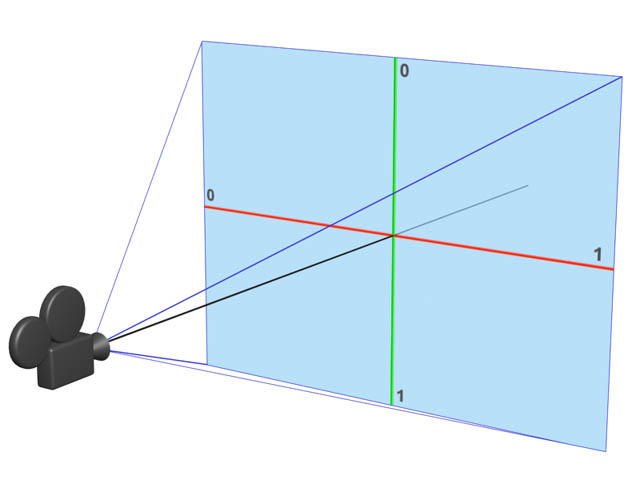
\includegraphics[width=9cm]{pics/camera01}
\end{center}
\end{methoddesc}

\begin{methoddesc}{getNearFar}{}
Return a 2-tuple (\var{near}, \var{far}) with the distances to the
near and far clipping planes. If automatic computation is disabled,
the method just returns the stored values, otherwise the values
are computed from the bounding box of the scene (which is converted
to a bounding sphere and the clipping planes are set as tangent planes
to the sphere).
\end{methoddesc}

% FreeCamera

\section{\class{FreeCamera} ---
         Free camera}

The \class{FreeCamera} class can be freely positioned and oriented in 
the scene.

\begin{classdesc}{FreeCamera}{name = "FreeCamera",\\ 
                       fov = 45.0,\\
                       target = None,\\
                       focallength = 0,\\
                       fstop = 0,\\
                       auto_nearfar = True,\\
                       nearplane = 0.1,\\
                       farplane = 1000.0,\\
                       }

\var{fov} is the field of view in degrees (in vertical direction), i.e.
the angle between the bottom and the top of the screen.

\var{target} is the point that the camera will initially look at. If no
target is specified the camera remains in its default orientation. Note
that the target is only used to compute an initial orientation. The
orientation will not be updated if the camera moves (use a 
\class{TargetCamera} if you want that behavior).

\var{focallength} is the focal length of the camera and \var{fstop} the
aperture number that determines the lens diameter. These values are used
to turn on depth of field. Depth of field is activated if both attributes
are set to a value different from 0 (note however, that not every renderer
supports depth of field). The focal distance is set so that the target 
point will always be in focus.

\var{auto_nearfar} specifies whether the near and far plane
distances are automatically determined or if fixed values are used.
If set to \code{False}, the \var{nearplane} and \var{farplane} arguments
are used, otherwise the values are computed from the objects in the scene.
In the latter case, the \var{nearplane} value still serves as minimum
value for the near plane distance which is used when the camera is located
within the scene bounds.
\end{classdesc}

The \class{FreeCamera} class has the following slots (in addition to
the slots of the \class{WorldObject} base class):

\begin{tableiv}{l|l|c|l}{code}{Slot}{Type}{Access}{Description}
\lineiv{fov_slot}{float}{rw}{Field of view in degrees}
\lineiv{focallength_slot}{float}{rw}{Focal length of the camera}
\lineiv{fstop_slot}{float}{rw}{Aperture number}
\lineiv{autonearfar_slot}{bool}{rw}{Automatically compute near/far values?}
\lineiv{nearplane_slot}{float}{rw}{(Minimal) near plane distance}
\lineiv{farplane_slot}{float}{rw}{Far plane distance}
\end{tableiv}

\begin{methoddesc}{projection}{width, height, near, far}
Returns the projection matrix for a viewport with the given width and
height (actually only the ratio width/height is relevant). The near
and far clipping planes are set to \var{near} and \var{far}.
\end{methoddesc}

\begin{methoddesc}{viewTransformation}{}
Returns the view transformation for this camera.
\end{methoddesc}

\begin{methoddesc}{eyeRay}{x0, y0, width, height}
Return a ray whose origin is at the eye position and that goes through
a given point on the image plane. The point on the plane is given by
(\var{x0}, \var{y0}) which each ranges from 0 to 1. (0,0) is at the
upper left and (1,1) at the lower right corner. The arguments \var{width} and
\var{height} determine the ratio of the image plane (the absolute
values of \var{width} and
\var{height} are irrelevant). The return value is a 2-tuple (\var{p}, \var{u})
where \var{p} is the ray origin and \var{u} the normalized
direction. Both vectors are given in world space.

\begin{center}
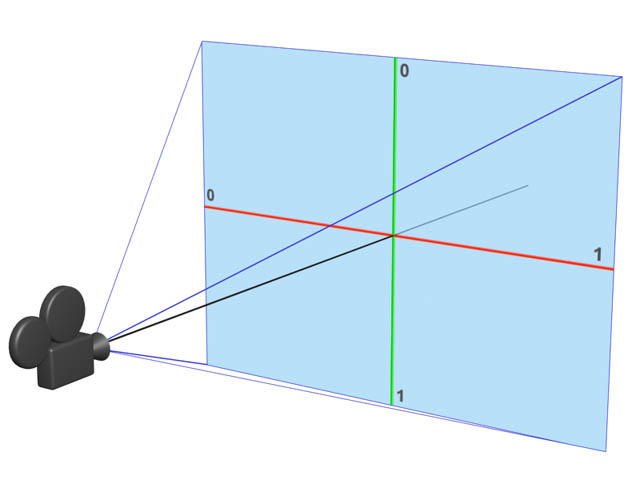
\includegraphics[width=9cm]{pics/camera01}
\end{center}
\end{methoddesc}

\begin{methoddesc}{getNearFar}{}
Return a 2-tuple (\var{near}, \var{far}) with the distances to the
near and far clipping planes. If automatic computation is disabled,
the method just returns the stored values, otherwise the values
are computed from the bounding box of the scene (which is converted
to a bounding sphere and the clipping planes are set as tangent planes
to the sphere).
\end{methoddesc}

% GLPointLight

\section{\class{GLPointLight} ---
         OpenGL point light}

\begin{classdesc}{GLPointLight}{name = ''GLPointLight'',\\ 
                       intensity = 1.0,\\
                       ambient = None,\\
                       diffuse = None,\\
                       specular = None,\\
                       constant_attenuation = 1.0,\\
                       linear_attenuation = 0.0,\\
                       quadratic_attenuation = 0.0,\\
                       enabled = True,\\
                       cast_shadow = False,\\
                       transform = None,\\
                       pos = None,\\
                       rot = None,\\
                       scale = None,\\
                       pivot = None,\\
                       offsetTransform = None,\\
                       auto_insert = True}

\end{classdesc}



% GLTargetSpotLight

\section{\class{GLTargetSpotLight} ---
         OpenGL target spot light}

\begin{classdesc}{GLTargetSpotLight}{name = ''GLTargetSpotLight'',\\ 
                       intensity = 1.0,\\
                       ambient = None,\\
                       diffuse = None,\\
                       specular = None,\\
                       constant_attenuation = 1.0,\\
                       linear_attenuation = 0.0,\\
                       quadratic_attenuation = 0.0,\\
                       exponent = 0.0,\\
                       cutoff = 45.0,\\
                       target = (0,0,0),\\
                       enabled = True,\\
                       cast_shadow = False,\\
                       transform = None,\\
                       pos = None,\\
                       rot = None,\\
                       scale = None,\\
                       pivot = None,\\
                       offsetTransform = None,\\
                       auto_insert = True}

\end{classdesc}



% GLFreeSpotLight

\section{\class{GLFreeSpotLight} ---
         OpenGL spot light}

\begin{classdesc}{GLFreeSpotLight}{name = ''GLFreeSpotLight'',\\ 
                       intensity = 1.0,\\
                       ambient = None,\\
                       diffuse = None,\\
                       specular = None,\\
                       constant_attenuation = 1.0,\\
                       linear_attenuation = 0.0,\\
                       quadratic_attenuation = 0.0,\\
                       exponent = 0.0,\\
                       cutoff = 45.0,\\
                       enabled = True,\\
                       cast_shadow = False,\\
                       transform = None,\\
                       pos = None,\\
                       rot = None,\\
                       scale = None,\\
                       pivot = None,\\
                       offsetTransform = None,\\
                       auto_insert = True}

\end{classdesc}



% GLTargetDistantLight

\section{\class{GLTargetDistantLight} ---
         OpenGL target distant light}

\begin{classdesc}{GLTargetDistantLight}{name = ''GLTargetDistantLight'',\\ 
                       intensity = 1.0,\\
                       ambient = None,\\
                       diffuse = None,\\
                       specular = None,\\
                       target = (0,0,0),\\
                       enabled = True,\\
                       cast_shadow = False,\\
                       transform = None,\\
                       pos = None,\\
                       rot = None,\\
                       scale = None,\\
                       pivot = None,\\
                       offsetTransform = None,\\
                       auto_insert = True}

\end{classdesc}



% GLFreeDistantLight

\section{\class{GLFreeDistantLight} ---
         OpenGL distant light}

\begin{classdesc}{GLFreeDistantLight}{name = ''GLFreeDistantLight'',\\ 
                       intensity = 1.0,\\
                       ambient = None,\\
                       diffuse = None,\\
                       specular = None,\\
                       enabled = True,\\
                       cast_shadow = False,\\
                       transform = None,\\
                       pos = None,\\
                       rot = None,\\
                       scale = None,\\
                       pivot = None,\\
                       offsetTransform = None,\\
                       auto_insert = True}

\end{classdesc}



% SpotLight3DS

\section{\class{SpotLight3DS} ---
         3DS spot light}

The \class{SpotLight3DS} class stores all parameters of the spot lights
as they are stored in 3DS files. The main purpose of this class is to
ensure that data doesn't get lost during file conversions.

This light sources can also be used for RenderMan renderings. However,
not all of the parameters are currently taken into account in the
corresponding RenderMan shader (see below).

\begin{classdesc}{SpotLight3DS}{name = "SpotLight3DS",\\ 
                       enabled = True,\\
                       intensity = 1.0,\\
                       color = (1,1,1),\\
                       see_cone = False,\\
                       roll = 0.0,\\
                       outer_range = 0,\\
                       inner_range = 0,\\
                       attenuation = 0,\\
                       rectangular_spot = 0,\\
                       shadowed = False,\\
                       shadow_bias = 0,\\
                       shadow_filter = 4.0,\\
                       shadow_size = 256,\\
                       spot_aspect = 0,\\
                       use_projector = False,\\
                       projector = 0,\\
                       overshoot = False,\\
                       ray_shadows = False,\\
                       ray_bias = False,\\
                       hotspot = 43,\\
                       falloff = 45,\\
	               target = (0,0,0)
                  }

\var{enabled} is a boolean flag that can be used to turn the light source
on or off.

\var{intensity} is the overall intensity of the light source. The higher
the value, the brighter the light.

\var{color} defines the color of the light source. It must be a sequence
of 3 floats containing RGB values.

\var{see_cone} ...

\var{roll} ...

\var{inner_range} and \var{outer_range} specify an intensity range based
on distance. Any parts of the scene that are nearer to the light source
than \var{inner_range} are fully illuminated. Within the range between
\var{inner_range} and \var{outer_range} the brightness drops off to 0
and objects further than \var{outer_range} are not illuminated at all.
These range values are only taken into account when \var{attenuation}
is not 0.

\var{rectangular_spot} ...

If \var{shadowed} is set to \code{True} the light casts a shadow.

\var{shadow_bias} is a small value greater than 0 that is used to prevent
invalid self-shadowing (i.e. so that a surface element doesn't shadow itself).

\var{shadow_filter} specifies the size of the filter when doing shadow map
lookups. The higher the value the blurrier the shadow.

\var{shadow_size} defines the size of the shadow map. The shadow map will
always be square and have a width of \var{shadow_size} pixels.

\var{spot_aspect} ...

\var{use_projector} ...

\var{projector} ...

If \var{overshoot} is \code{True} the light virtually becomes a point light
source, i.e. it also illuminates the parts of the scene that lie outside
its cone but the shadow is still restricted to the cone.

\var{ray_shadows} ...

\var{ray_bias} ...

\var{hotspot} This is the angle (in degrees) of the "inner" cone which is fully illuminated.

\var{falloff} This is the angle (in degrees) of the "outer" cone. The light 
intensity between the inner and outer cone drops off to 0. The region outside
the outer cone is not illuminated (unless \var{overshoot} is activated).

\var{target} is the target point that the light source aims at.

\end{classdesc}

The following parameters are used in the corresponding RenderMan
shader, all other parameters are currently ignored:

\begin{itemize}
\item intensity
\item color
\item falloff
\item hotspot
\item attenuation
\item inner_range
\item outer_range
\item overshoot
\item shadow_bias
\item shadow_filter
\item shadow_size
\end{itemize}

% SpotLight3DS

\section{\class{RMLightSource} ---
         RenderMan light source}

\begin{classdesc}{RMLightSource}{name = "RMLightSource",\\ 
                       shader = None
                  }


\var{shader} specifies the light shader that should be used. It
can either be a string containing the shader name or a \class{RMShader}
instance representing the shader (see section \ref{rmshader}).

\end{classdesc}


The parameters of the shader is made available as attributes of the
light source object. The corresponding slots can be obtained by adding
the suffix \code{_slot} to the name.


% RIBArchive component

\section{\class{RIBArchive} ---
         Reference an external RIB archive}

The \class{RIBArchive} class represents geometry that is defined in
an external RIB file. When the scene is rendered using a RenderMan
renderer the RIB file will be included via a call to 
\cfunction{RiReadArchive()}. In an interactive viewer, a \class{RIBArchive}
object will be invisible.

\begin{classdesc}{RIBArchive}{name = "RIBArchive",\\ 
                              filename = None, \\
                              auto_insert = True}

\var{filename} is the name of the external RIB file.

\end{classdesc}



% ODE joints

\section{ODE joints ---
         Joint classes for the ODEDynamics component}

%----------------------------------------------------------------------
\subsection{\class{ODEBallJoint} --- Ball and socket joint}

\begin{classdesc}{ODEBallJoint}{name = "ODEBallJoint",\\ 
                             body1 = None, \\
                             body2 = None
                             }

\end{classdesc}

%----------------------------------------------------------------------
\subsection{\class{ODEHingeJoint} --- Hinge joint}

\begin{classdesc}{ODEHingeJoint}{name = "ODEHingeJoint",\\ 
                             body1 = None, \\
                             body2 = None
                             }

\end{classdesc}

%----------------------------------------------------------------------
\subsection{\class{ODESliderJoint} --- Slider joint}

\begin{classdesc}{ODESliderJoint}{name = "ODESliderJoint",\\ 
                             body1 = None, \\
                             body2 = None
                             }

\end{classdesc}

%----------------------------------------------------------------------
\subsection{\class{ODEHinge2Joint} --- Hinge-2 joint}

\begin{classdesc}{ODEHinge2Joint}{name = "ODEHinge2Joint",\\ 
                             body1 = None, \\
                             body2 = None
                             }

\end{classdesc}

%----------------------------------------------------------------------
\subsection{\class{ODEUniversalJoint} --- Universal joint}

\begin{classdesc}{ODEUniversalJoint}{name = "ODEUniversalJoint",\\ 
                             body1 = None, \\
                             body2 = None
                             }

\end{classdesc}




% BezierCurve

\section{\class{BezierCurve} ---
         Bezier curve}

\begin{classdesc}{BezierCurve}{name = "BezierCurve",\\ 
                               pnts = None,\\
                               closed = False,\\
                               epsilon = 0.01,\\
                               subdiv = 4,\\
                               show_tangents = False,\\
                               curvegeom = None\\
                              }

\var{pnts} is a list of \class{BezierPoint} objects (see section
\ref{beziercurvegeom}).

If \var{closed} is set to \code{True} the last point will be connected
to the first point.

\var{epsilon} is a threshold value that determines the accuracy of
length calculations of the curve.

\var{subdiv} is the number of subdivisions that are made to draw the
curve using OpenGL.

If \var{show_tangents} is set to \code{True} the OpenGL visualization
will also show the in and out tangents.

You can also pass a previously created \class{BezierCurveGeom} object
via the \var{curvegeom} argument. In this case, the arguments \var{pnts},
\var{closed}, \var{epsilon}, \var{subdiv} and \var{show_tangents} are 
ignored.
\end{classdesc}





%---
\chapter{GeomObjects \label{geomobjects}}

% GeomObject

\section{\class{GeomObject} ---
         Geometry base class}

The \class{GeomObject} class is the base class for all geometries.
Instances of this class are stored in the \member{geom} attribute
of the world objects and can be shared among them.

\begin{classdesc}{GeomObject}{}
...params?...
\end{classdesc}

% Methods
\begin{methoddesc}{boundingBox}{}
Return the local axis aligned bounding box. The bounding box is
given with respect to the local transformation L (which is not
what you get from the transform slot of the world object).
\end{methoddesc}

\begin{methoddesc}{drawGL}{}
Draw the geometry using OpenGL commands.
\end{methoddesc}

\begin{methoddesc}{uniformCount}{}
Return the multiplicity of \keyword{UNIFORM} variables.
\end{methoddesc}

\begin{methoddesc}{varyingCount}{}
Return the multiplicity of \keyword{VARYING} variables.
\end{methoddesc}

\begin{methoddesc}{vertexCount}{}
Return the multiplicity of \keyword{VERTEX} variables.
\end{methoddesc}

\begin{methoddesc}{faceVaryingCount}{}
Return the multiplicity of \keyword{FACEVARYING} variables.
\end{methoddesc}

\begin{methoddesc}{faceVertexCount}{}
Return the multiplicity of \keyword{FACEVERTEX} variables.
\end{methoddesc}

\begin{methoddesc}{slotSizeConstraint}{storage}
Return a constraint object for primitive variable slots or None if the size
of the slot should be unconstrained.
This method is called when a new primitive variable is created. The
returned constraint object is used for the array slot that holds the
values of the variable. \var{storage} is the storage class of the new
variable which will be one of \code{UNIFORM}, \code{VARYING}, \code{VERTEX},
\code{FACEVARYING} or \code{FACEVERTEX}. The method will never be called
when \code{CONSTANT} or \code{USER} variables are created.
\end{methoddesc}

\begin{methoddesc}{newVariable}{name, storage, type, multiplicity=1, user_n=0}
Attaches a new primitive variable to the geometry.

\var{storage} specifies the storage
class, i.e. how many values are actually stored. It must be one of
\code{CONSTANT}, \code{UNIFORM}, \code{VARYING}, \code{VERTEX}, 
\code{FACEVARYING}, \code{FACEVERTEX} or
\code{USER}. The exact number of values depends on the actual geometry.
However, \code{CONSTANT} is always exactly one value for the entire
geometry and \code{USER} is a user defined number specified in \var{user_n}.

\var{type} is the type of the variable and must be one of 
\code{INT}, \code{FLOAT}, \code{STRING}, \code{COLOR}, \code{POINT}, 
\code{VECTOR}, \code{NORMAL}, \code{MATRIX} and \code{HPOINT}. 
If \var{multiplicity} is greater than 1, then an array with that size is
created. 

Creating a new variable will always create a new slot of that name as well.
The slot is always an \class{ArraySlot} (even for \code{CONSTANT} variables).
After you have created a variable you can use the corresponding slot to
manipulate the values of the variable.

Here is an example of a "varying int [3]" variable that's created on a sphere 
geometry. This means, the variable will consist of four 3-tuples of integers
(one for each parametric corner).

\begin{verbatim}
>>> from cgkit.all import *
>>> sg=SphereGeom()
>>> sg.newVariable("foo", VARYING, INT, multiplicity=3)
>>> for v in sg.iterVariables(): print v
...
('foo', cgkit._core.VarStorage.VARYING, cgkit._core.VarType.INT, 3)
>>> s=sg.slot("foo")
>>> s[1]=(1,2,3)
>>> for f in s: print f
...
(0, 0, 0)
(1, 2, 3)
(0, 0, 0)
(0, 0, 0)
\end{verbatim}
\end{methoddesc}

\begin{methoddesc}{deleteVariable}{name}
Delete the primitive variable with the specified name.
\end{methoddesc}

\begin{methoddesc}{deleteAllVariables}{}
Delete all primitive variables.
\end{methoddesc}

\begin{methoddesc}{findVariable}{name}
Search for a particular primitive variable and return its descriptor.
\code{None} is returned if a variable called \var{name} cannot be found.
The return value is a 4-tuple (name, storage class, type, multiplicity)
describing the variable. See the \method{newVariable()} method for a
description of the individual elements.
\end{methoddesc}

\begin{methoddesc}{iterVariables}{}
Return an iterator that iterates over all existing primitive variables.
The iterator will return the same 4-tuple as returned by 
\method{findVariable()}.
\end{methoddesc}

\begin{methoddesc}{convert}{targetgeom}
Convert the geometry into another type of geometry. \var{targetgeom}
is another \class{GeomObject} that will receive the result of the
conversion.  If the conversion is not possible, a
\exception{NotImplementedError} exception is thrown.

In the following example, a box geometry is converted into a triangle
mesh:

\begin{verbatim}
>>> bg=BoxGeom(segmentsx=3, segmentsy=3, segmentsz=3)
>>> tm=TriMeshGeom()
>>> bg.convert(tm)
>>> print len(tm.verts)
56
>>> print len(tm.faces)
108
\end{verbatim}
\end{methoddesc}




% BoxGeom

\section{\class{BoxGeom} ---
         Box geometry}

\begin{classdesc}{BoxGeom}{lx=1.0, ly=1.0, lz=1.0, segmentsx=1, segmentsy=1, segmentsz=1}

\var{lx}, \var{ly} and \var{lz} specify the dimensions of the box in
the respective direction.

\var{segmentsx}, \var{segmentsy} and \var{segmentsz} are the number of
segments in each direction.
\end{classdesc}

A \class{BoxGeom} has the following slots:

\begin{tableiv}{l|l|c|l}{code}{Slot}{Type}{Access}{Description}
\lineiv{cog_slot}{vec3}{r}{The local center of gravity}
\lineiv{inertiatensor_slot}{mat3}{r}{The local inertia tensor}
\lineiv{lx_slot}{float}{rw}{The length in x direction}
\lineiv{ly_slot}{float}{rw}{The length in y direction}
\lineiv{lz_slot}{float}{rw}{The length in z direction}
\lineiv{segmentsx_slot}{int}{rw}{The number of segments in x direction}
\lineiv{segmentsy_slot}{int}{rw}{The number of segments in y direction}
\lineiv{segmentsz_slot}{int}{rw}{The number of segments in z direction}
\end{tableiv}

% Attributes
\begin{memberdesc}{cog}
Center of gravity with respect to the local coordinate system.
\end{memberdesc}

\begin{memberdesc}{inertiatensor}
Inertia tensor with respect to the local coordinate system.
\end{memberdesc}

\begin{memberdesc}{lx}
The length in x direction.
\end{memberdesc}

\begin{memberdesc}{ly}
The length in y direction.
\end{memberdesc}

\begin{memberdesc}{lz}
The length in z direction.
\end{memberdesc}

\begin{memberdesc}{segmentsx}
The number of segments in x direction.
\end{memberdesc}

\begin{memberdesc}{segmentsy}
The number of segments in y direction.
\end{memberdesc}

\begin{memberdesc}{segmentsz}
The number of segments in z direction.
\end{memberdesc}








% SphereGeom

\section{\class{SphereGeom} ---
         Sphere geometry}

\begin{classdesc}{SphereGeom}{radius=1.0, segmentsu=16, segmentsv=8}
\var{radius} is the radius in the local coordinate system.

\var{segmentsu} and \var{segmentsv} are used when the sphere has to
be tesselated (either for interactive display or when converted to
a triangle mesh).
\end{classdesc}

A \class{SphereGeom} has the following slots:

\begin{tableiv}{l|l|c|l}{code}{Slot}{Type}{Access}{Description}
\lineiv{cog_slot}{vec3}{r}{The local center of gravity}
\lineiv{inertiatensor_slot}{mat3}{r}{The local inertia tensor}
\lineiv{radius_slot}{float}{rw}{The radius}
\lineiv{segmentsu_slot}{int}{rw}{The number of segments in u direction}
\lineiv{segmentsv_slot}{int}{rw}{The number of segments in v direction}
\end{tableiv}

% Attributes
\begin{memberdesc}{cog}
Center of gravity with respect to the local coordinate system.
\end{memberdesc}

\begin{memberdesc}{inertiatensor}
Inertia tensor with respect to the local coordinate system.
\end{memberdesc}

\begin{memberdesc}{radius}
The radius of the sphere.
\end{memberdesc}

\begin{memberdesc}{segmentsu}
The number of segments in u direction.
\end{memberdesc}

\begin{memberdesc}{segmentsv}
The number of segments in v direction.
\end{memberdesc}







% CCylinderGeom

\section{\class{CCylinderGeom} ---
         Capped cylinder geometry}

\begin{classdesc}{CCylinderGeom}{radius=1.0, length=1.0, segmentsu=16, segmentsvl=1, segmentsvr=4}

\var{radius} is the radius of the cylinder and caps in the local coordinate 
system.

\var{length} is the length of the cylinder (not counting the caps).

\var{segmentsu} is the number of segments in u direction, \var{segmentsvl}
the number of segments of the cylinder part and \var{segmentsvr} the
number of segments for each cap.
\end{classdesc}

A \class{CCylinderGeom} has the following slots:

\begin{tableiv}{l|l|c|l}{code}{Slot}{Type}{Access}{Description}
\lineiv{cog_slot}{vec3}{r}{The local center of gravity}
\lineiv{inertiatensor_slot}{mat3}{r}{The local inertia tensor}
\lineiv{radius_slot}{float}{rw}{The radius of the cylinder}
\lineiv{length_slot}{float}{rw}{The lenght of the cylinder}
\lineiv{segmentsu_slot}{int}{rw}{The number of segments in u direction}
\lineiv{segmentsvl_slot}{int}{rw}{The number of cylinder segments in v direction}
\lineiv{segmentsvr_slot}{int}{rw}{The number of cap segments in v direction}
\end{tableiv}

% Attributes
\begin{memberdesc}{cog}
Center of gravity with respect to the local coordinate system.
\end{memberdesc}

\begin{memberdesc}{inertiatensor}
Inertia tensor with respect to the local coordinate system.
\end{memberdesc}

\begin{memberdesc}{radius}
The radius of the cylinder and caps.
\end{memberdesc}

\begin{memberdesc}{length}
The length of the cylinder (not counting the caps).
\end{memberdesc}

\begin{memberdesc}{segmentsu}
The number of segments in u direction.
\end{memberdesc}

\begin{memberdesc}{segmentsvl}
The number of cylinder segments in v direction.
\end{memberdesc}

\begin{memberdesc}{segmentsvr}
The number of cap segments in v direction.
\end{memberdesc}

% PlaneGeom

\section{\class{PlaneGeom} ---
         Plane geometry}

\begin{classdesc}{PlaneGeom}{lx=1.0, ly=1.0, segmentsx=1, segmentsy=1}

\var{lx} and \var{ly} specify the dimensions of the plane in
the respective direction.

\var{segmentsx} and \var{segmentsy} are the number of
segments in each direction.
\end{classdesc}

A \class{PlaneGeom} has the following slots:

\begin{tableiv}{l|l|c|l}{code}{Slot}{Type}{Access}{Description}
\lineiv{lx_slot}{float}{rw}{The length in x direction}
\lineiv{ly_slot}{float}{rw}{The length in y direction}
\lineiv{segmentsx_slot}{int}{rw}{The number of segments in x direction}
\lineiv{segmentsy_slot}{int}{rw}{The number of segments in y direction}
\end{tableiv}

% Attributes
\begin{memberdesc}{lx}
The length in x direction.
\end{memberdesc}

\begin{memberdesc}{ly}
The length in y direction.
\end{memberdesc}

\begin{memberdesc}{segmentsx}
The number of segments in x direction.
\end{memberdesc}

\begin{memberdesc}{segmentsy}
The number of segments in y direction.
\end{memberdesc}







% TorusGeom

\section{\class{TorusGeom} ---
         Torus geometry}

\begin{classdesc}{TorusGeom}{major=1.0, minor=0.1, segmentsu=16, segmentsv=8}
\end{classdesc}








% TriMeshGeom

\section{\class{TriMeshGeom} ---
         Triangle mesh geometry}

\begin{classdesc}{TriMeshGeom}{}
Creates an empty triangle mesh.
\end{classdesc}

A \class{TriMeshGeom} has the following slots:

\begin{tableiv}{l|l|c|l}{code}{Slot}{Type}{Access}{Description}
\lineiv{cog_slot}{vec3}{r}{The local center of gravity}
\lineiv{inertiatensor_slot}{mat3}{r}{The local inertia tensor}
\lineiv{verts_slot}{vec3 array}{rw}{The mesh vertices}
\lineiv{faces_slot}{int[3] array}{rw}{The mesh faces}
\end{tableiv}

% Attributes
\begin{memberdesc}{cog}
Center of gravity with respect to the local coordinate system of the 
triangle mesh.
\end{memberdesc}

\begin{memberdesc}{inertiatensor}
Inertia tensor with respect to the local coordinate system of the 
triangle mesh.
\end{memberdesc}

\begin{memberdesc}{verts}
This attribute contains the sequence of mesh vertices.
\end{memberdesc}

\begin{memberdesc}{faces}
This attribute contains the sequence of mesh faces. Each face contains
three vertex indices.
\end{memberdesc}

% Methods
\begin{methoddesc}{intersectRay}{origin, direction, earlyexit=False}
Intersect a ray with the mesh. The ray starts at \var{origin} and
travels along \var{direction} which must both be of type \class{vec3}.
\var{origin} and \var{direction} must be given with respect to the
local coordinate system L of the geometry. If \var{earlyexit} is
\code{True} the method returns after the first hit, otherwise all
triangles are tested and the result contains the nearest hit.
The return value is a tuple (\var{hit}, \var{t}, \var{faceindex}, 
\var{u}, \var{v}) where \var{hit} is a boolean that indicates if
the mesh was hit or not. \var{t} is the ray parameter, i.e. the
point of intersection is at \var{origin} + t*\var{direction}.
\var{faceindex} is the index of the face that was hit and \var{u}
\var{v} are the parameter coordinates of the intersection point.

This method tests the ray with all triangles, so it is not efficient if
you have a lot of rays to test. It is meant for only a few rays where
the preprocessing cost wouldn't be amortized.
 
The ray-triangle intersection code (non-culling case) is based on:
 
Tomas M�ller and Ben Trumbore\\
{\em Fast, minimum storage ray-triangle intersection}\\
Journal of graphics tools, 2(1):21-28, 1997\\
\url{http://www.acm.org/jgt/papers/MollerTrumbore97/}
\end{methoddesc}






% PolyhedronGeom

\section{\class{PolyhedronGeom} ---
         Polyhedron geometry}

The \class{PolyhedronGeom} class stores a collection of general planar
concave polygons that may also contain holes. Each polygon is described
by a sequence of vertex loops. The first loop defines the polygon boundary
and each subsequent loop describes a hole. Each loop is a sequence of
vertex indices.

\begin{classdesc}{PolyhedronGeom}{}
Creates an empty polyhedron.
\end{classdesc}

A \class{PolyhedronGeom} has the following slots:

\begin{tableiv}{l|l|c|l}{code}{Slot}{Type}{Access}{Description}
\lineiv{verts_slot}{vec3 array}{rw}{The polygon vertices}
\end{tableiv}

% Attributes
\begin{memberdesc}{verts}
This attribute contains the sequence of polygon vertices.
\end{memberdesc}

% Methods
\begin{methoddesc}{hasPolysWithHoles}{}
Return \code{True} if there is at least one polygon with a hole.
\end{methoddesc}

\begin{methoddesc}{getNumPolys}{}
Return the number of polygons.
\end{methoddesc}

\begin{methoddesc}{getNumLoops}{poly}
Return the number of vertex loops in the polygon with index \var{poly}.
\end{methoddesc}

\begin{methoddesc}{getNumVerts}{poly, loop}
Return the number of vertex indices in one particular loop. \var{poly}
is the polygon index and \var{loop} the loop index.
\end{methoddesc}

\begin{methoddesc}{setNumPolys}{num}
Allocate space for \var{num} polygons.
\end{methoddesc}

\begin{methoddesc}{setNumLoops}{poly, num}
Allocate space for \var{num} loops in the polygon with index \var{poly}.
\end{methoddesc}

\begin{methoddesc}{getLoop}{poly, loop}
Return a loop from a polygon. \var{poly} is the polygon index and \var{loop}
the loop index. The return value is a sequence of vertex indices.
\end{methoddesc}

\begin{methoddesc}{setLoop}{poly, loop, vloop}
Set a new polygon loop. \var{poly} is the polygon index, \var{loop}
the loop index and \var{vloop} a sequence of vertex indices.
\end{methoddesc}

\begin{methoddesc}{getPoly}{poly}
Return a polygon. \var{poly} is the polygon index. The return value
is a sequence of vertex loops.
\end{methoddesc}

\begin{methoddesc}{setPoly}{poly, polydef}
Set a polygon. \var{poly} is the polygon index and \var{polydef} a sequence
of vertex loops.
\end{methoddesc}





% BezierCurveGeom

\section{\class{BezierCurveGeom} ---
         Piecewise cubic Bezier curve}
\label{beziercurvegeom}

The \class{BezierCurveGeom} class represents a piecewise cubic curve
in 3D space that is composed of an arbitrary number of cubic Bezier
segments. The class stores a number of 3D points that are interpolated
by the curve. Each point has an in tangent and an out tangent associated
with it that define how the curve enters and leaves the point.

\begin{classdesc}{BezierPoint}{pos, intangent=vec3(0), outtangent=vec3(0)}

This class just stores a position and the in and out tangents and
is used to pass these parameters to the constructor of a 
\class{BezierCurveGeom}.

\var{pos} is a point position that the curve will interpolate.

\var{intangent} and \var{outtangent} define where the curve enters
and leaves the point.
\end{classdesc}


\begin{classdesc}{BezierCurveGeom}{pnts = None,\\
                                   closed = False,\\
                                   epsilon = 0.01,\\
                                   subdiv = 4,\\
                                   show_tangents = False}

\var{pnts} is a list of \class{BezierPoint} objects describing the
points to interpolate and the in and out tangents.

If \var{closed} is set to \code{True} the last point will be connected
to the first point.

\var{epsilon} is a threshold value that determines the accuracy of
length calculations of the curve.

\var{subdiv} is the number of subdivisions that are made to draw the
curve using OpenGL.

If \var{show_tangents} is set to \code{True} the OpenGL visualization
will also show the in and out tangents.
\end{classdesc}

A \class{BezierCurveGeom} has the following slots:

\begin{tableiv}{l|l|c|l}{code}{Slot}{Type}{Access}{Description}
\lineiv{pnts_slot}{[vec3]}{rw}{The curve points}
\lineiv{intangents_slot}{[vec3]}{rw}{The in tangents}
\lineiv{outtangents_slot}{[vec3]}{rw}{The out tangents}
\end{tableiv}

\begin{memberdesc}{closed}
This is a boolean indicating wheter the curve is closed or not. You
can read and write this attribute.
\end{memberdesc}

\begin{memberdesc}{numsegs}
The number of Bezier segments in the curve. You can only read this
attribute.
\end{memberdesc}

\begin{memberdesc}{paraminterval}
This is a tuple (\var{t_min}, \var{t_max}) containing the valid parameter
interval of the curve. You can only read this attribute.
\end{memberdesc}

% eval
\begin{methoddesc}{eval}{t}
Evaluate the curve at parameter \var{t} and return the curve point.
\end{methoddesc}

% evalFrame
\begin{methoddesc}{evalFrame}{t}
Evaluate the curve at parameter \var{t} and return the curve point,
the tangent and the second derivative.
\end{methoddesc}

% deriv
\begin{methoddesc}{deriv}{t}
Return the first derivative (the tangent) at parameter \var{t}.
\end{methoddesc}

% arcLen
\begin{methoddesc}{arcLen}{t}
Return the arc length of the curve up to the point specified by the parameter
\var{t}.
\end{methoddesc}

% length
\begin{methoddesc}{length}{}
Return the entire length of the curve. This is equivalent to 
\code{arcLen(t_max)}.
\end{methoddesc}








%---
\chapter{Materials \label{materials}}

% GLMaterial

\section{\class{GLMaterial} ---
         OpenGL material}

The \class{GLMaterial} class represents the material model of the standard
OpenGL API. All colors are represented as (r,g,b,a). If you don't use
blending you can leave out the alpha value in the constructor.

\begin{classdesc}{GLMaterial}{name = "GLMaterial",\\ 
                              ambient = (0.2, 0.2, 0.2, 1.0),\\
                              diffuse = (0.7, 0.7, 0.7, 1.0),\\
                              specular = (0, 0, 0, 1),\\
                              shininess = 0.0,\\
                              emission = (0, 0, 0, 1),\\
                              blend_factors = None,\\
                              texture = None,\\
                              vertex_shader = None,\\
                              fragment_shader = None,\\
                              density = 1.0}

\var{ambient} is the ambient color of the material.

\var{diffuse} is the diffuse color of the material.

\var{specular} is the color of the specular highlight.

\var{shininess} determines the size of the highlight and lies 
between 0.0 and 128.0. The higher the value, the smaller and brighter
the highlight.

The \var{emission} color can be used to simulate objects that emit light.

\var{blend_factors} is a 2-tuple with the parameters for the 
\cfunction{glBlendFunc()} call which indicate how to compute the
source and destination blend factors 
(see \ulink{\cfunction{glBlendFunc()}}{http://pyopengl.sourceforge.net/documentation/manual/glBlendFunc.3G.html}).
Blending is disabled if \var{blend_factors} is \code{None}.

\var{texture} is either \code{None}, a single \class{GLTexture} object or
a list of \class{GLTexture} objects specifying the texture image(s) to use.

\var{vertex_shader} is either \code{None}, a single \class{GLShader} object
or a list of \class{GLShader} objects specifying the vertex shaders to use.

\var{fragment_shader} is either \code{None}, a single \class{GLShader} object
or a list of \class{GLShader} objects specifying the fragment shaders to use.

\var{density} is the density value used for physical simulations.
\end{classdesc}

% Methods
\begin{methoddesc}{getNumTextures}{}
Return the current size of the texture array.
\end{methoddesc}

\begin{methoddesc}{setNumTextures}{num}
Set a new size for the texture array.
\end{methoddesc}

\begin{methoddesc}{getTexture}{idx=0}
Get a stored texture. The method returns \code{None} if the given index
is out of range or if there is no texture stored at that position.
\end{methoddesc}

\begin{methoddesc}{setTexture}{tex, idx=0}
Set a new texture. An \exception{IndexError} exception is thrown if the 
index is out of range.
\end{methoddesc}

\begin{methoddesc}{getNumVertexShaders}{}
Return the current size of the vertex shader array.
\end{methoddesc}

\begin{methoddesc}{setNumVertexShaders}{num}
Set a new size for the vertex shader array.
\end{methoddesc}

\begin{methoddesc}{getVertexShader}{idx=0}
Get a vertex shader object. The method returns \code{None} if the given index
is out of range or if there is no shader object stored at that position.
\end{methoddesc}

\begin{methoddesc}{setVertexShader}{shader, idx=0}
Set a new vertex shader object. An \exception{IndexError} exception is 
thrown if the index is out of range. A ValueError exception is thrown if the 
shader is not of type \code{VERTEX}.
\end{methoddesc}

\begin{methoddesc}{getNumFragmentShaders}{}
Return the current size of the fragment shader array.
\end{methoddesc}

\begin{methoddesc}{setNumFragmentShaders}{num}
Set a new size for the fragment shader array.
\end{methoddesc}

\begin{methoddesc}{getFragmentShader}{idx=0}
Get a fragment shader object. The method returns \code{None} if the given index
is out of range or if there is no shader object stored at that position.
\end{methoddesc}

\begin{methoddesc}{setFragmentShader}{shader, idx=0}
Set a new fragment shader object. An \exception{IndexError} exception is 
thrown if the index is out of range. A ValueError exception is thrown if the 
shader is not of type \code{FRAGMENT}.
\end{methoddesc}

%-----------------------
\subsection{\class{GLTexture} --- Specifying a texture map}

The \class{GLTexture} class is used to describe the parameters of an
OpenGL texture map for use with the \class{GLMaterial} class.

\begin{classdesc}{GLTexture}{imagename = "",\\
                             image = None,\\ 
                             mode = GL_DECAL,\\
                             mipmap = True,\\
                             mag_filter = GL_LINEAR,\\
                             min_filter = GL_LINEAR,\\
                             wrap_s = GL_REPEAT,\\
                             wrap_t = GL_REPEAT,\\
                             internalformat = GL_RGB,\\
                             texenvcolor = vec4(1),\\
                             transform = mat4(1),\\
                             size = None, \\
                             environment_map = False\\
                            }

\var{imagename} is the name of the image file that should be used as a
texture map. If the image resolution is not a power of 2, the image
is scaled up to the next higher power of 2 resolution.

It is also possible to pass the actual image data in the \var{image}
parameter.  The image can either be a PIL image or the raw RGB
data. In the latter case, you must explicitly specify the image
resolution (which must then be a power of 2 resolution) in the \var{size}
argument. The \var{imagename} argument is ignored if the data is passed
via the \var{image} argument.

\var{mode} specifies how the image is applied to the object. It can be
one of \code{GL_REPLACE}, \code{GL_MODULATE}, \code{GL_DECAL} and 
\code{GL_BLEND}. In the latter
case, the blend color is given by \var{texenvcolor} 
(see \ulink{\cfunction{glTexEnv()}}{http://pyopengl.sourceforge.net/documentation/manual/glTexEnv.3G.html}).

\var{mipmap} determines whether mip mapping should be used or not.

\var{mag_filter} is the filter to use when magnification occurs (i.e. when
the texture appears larger on screen that it actually is). It can be
either \code{GL_NEAREST} or \code{GL_LINEAR}.

\var{min_filter} is the filter to use when minification occurs (i.e. when
the texture appears smaller on screen that it actually is). It can be one
of following values
(see \ulink{\cfunction{glTexParameter()}}{http://pyopengl.sourceforge.net/documentation/manual/glTexParameter.3G.html}):
%\code{GL_NEAREST}, \code{GL_LINEAR}, \code{GL_NEAREST_MIPMAP_NEAREST},
%\code{GL_NEAREST_MIPMAP_LINEAR}, \code{GL_LINEAR_MIPMAP_NEAREST} or
%\code{GL_LINEAR_MIPMAP_LINEAR}

\begin{itemize}
\item \code{GL_NEAREST}
\item \code{GL_LINEAR}
\item \code{GL_NEAREST_MIPMAP_NEAREST}
\item \code{GL_NEAREST_MIPMAP_LINEAR}
\item \code{GL_LINEAR_MIPMAP_NEAREST}
\item \code{GL_LINEAR_MIPMAP_LINEAR}
\end{itemize}

If \code{GL_LINEAR} is specified and mip mapping
is used then the filter is automatically set to \code{GL_LINEAR_MIPMAP_LINEAR}

\var{wrap_s} and \var{wrap_t} specify what happens if the texture coordinate
leave the range 0-1. They can be one of \code{GL_REPEAT}, \code{GL_CLAMP}
and \code{GL_CLAMP_TO_EDGE}
(see \ulink{\cfunction{glTexParameter()}}{http://pyopengl.sourceforge.net/documentation/manual/glTexParameter.3G.html}).

\var{internalformat} specifies how the image data will be stored in memory.
Usually, you'll either specify \code{GL_RGB} or \code{GL_RGBA} if you have
alpha values in your image and you want to use them
(see \ulink{\cfunction{glTexImage2D()}}{http://pyopengl.sourceforge.net/documentation/manual/glTexImage2D.3G.html}).

\var{transform} is a transformation that is applied to the texture coordinates.

\var{size} is a 2-tuple containing the desired texture map resolution which
must be a power of 2. The image is resized to the specified resolution.
If \var{size} is \code{None} then the next higher power of 2 value is used.

If \var{environment_map} is \code{True} the image is used as a 
latitude/longitude environment map.

\end{classdesc}

%-----------------------
\subsection{\class{GLShader} --- Specifying a shader}

The \class{GLShader} class is used to add a OpenGL 2 shader source file
to a \class{GLMaterial} class.

\begin{classdesc}{GLShader}{shadertype,\\
                            filename,\\ 
                            cpp = None,\\
                            cpperrstream = sys.stderr,\\
                            **shaderparams
                            }

\var{shadertype} specifies whether this shader is vertex shader or a
fragment shader. The value can either be \code{GLShader.ShaderType.VERTEX}
(or \code{GLSLANG_VERTEX}) or \code{GLShader.ShaderType.FRAGMENT}
(or \code{GLSLANG_FRAGMENT}).

\var{filename} is the shader source file name.

\var{cpp} determines the preprocessor that should be used when extracting
shader parameters. \var{cpperrstream} is used to output errors from the
preprocessor (see the function \function{glslangparams.glslangparams()} 
(section \ref{glslangparams}) for details).

Any additional keyword argument is assumed to be a shader parameter.
\end{classdesc}


% RMMaterial

\section{\class{RMMaterial} ---
         RenderMan material}

The \class{RMMaterial} class is a special material that is only of
use if you are creating images via a RenderMan renderer and you want
to write your shaders in external shader files or use shaders that
are already compiled.

The material may consist of a surface shader, a displacement shader
and an interior shader. The shader source files (or only the shader
names) are passed via \class{RMShader} instances as arguments to the
constructor. If the \class{RMShader} instance points to a file, the
material object will take care of the compilation of the
file. Otherwise, it is up to you to compile the shader and make sure
that the renderer can find it.

\begin{classdesc}{RMMaterial}{name = "RMMaterial", \\
                              surface = None,\\
                              displacement = None,\\
                              displacementbound = ("current", 0.0),\\
                              interior = None,\\
                              color = None,\\
                              opacity = None
                             }


\var{surface} specifies the surface shader to use. It can either be
a string containing the shader name or a \class{RMShader} instance
representing the shader. You can also pass \code{None} if no surface
shader should be instantiated.

\var{displacment} specifies the displacment shader to use. It can either be
a string containing the shader name or a \class{RMShader} instance
representing the shader. You can also pass \code{None} if no displacment
shader should be instantiated.

\var{displacementbound} is a tuple (coordinate system, distance) that
specifies the maximum displacement. The distance is the maximum amount that
a surface point is displaced and  is given in the specified coordinate 
system.

\var{interior} specifies the interior shader to use. It can either be
a string containing the shader name or a \class{RMShader} instance
representing the shader. You can also pass \code{None} if no interior
shader should be instantiated.

\var{color} is the color that should be set via \cfunction{RiColor()}.

\var{opacity} is the opacity that should be set via \cfunction{RiOpacity()}.
\end{classdesc}

The parameters of the shaders are made available as attributes of the
material objects. The corresponding slots can be obtained by adding
the suffix \code{_slot} to the name. Attribute names in the surface shader
have priority over the attributes in the displacement shader which in
turn has priority over the interior shader. This means, if there are
identical parameter names in all shaders you will access the parameter
of the surface shader. You can also access the attributes of each
shader via the \var{surface}, \var{displacement} and \var{interior}
attributes which contain the corresponding \class{RMShader} instances.

Example:
   
\begin{verbatim}
mat = RMMaterial(surface = RMShader("mysurface.sl"),
                 displacement = RMShader("c:\\shaders\\dented.sl"),
                 color = (1,0.5,0.8)
                 )
...
Sphere(pos=(1,2,3), radius=0.5, material=mat)
\end{verbatim}

In this example, the material uses the surface shader \file{mysurface.sl}
and the displacement shader \file{c:\textbackslash shaders\textbackslash dented.sl}. The shaders will
be compiled automatically because the shader source files are given
(instead of just the shader names).

%------------------------------------------------------------
\subsection{\class{RMShader} ---  RenderMan shader}
\label{rmshader}

The \class{RMShader} class encapsulates a single RenderMan shader.

\begin{classdesc}{RMShader}{shader = None, \\
                            transform = mat4(1), \\
                            cpp = None, \\
                            cpperrstream = sys.stderr, \\
                            params = None, \\
                            paramlist}
	
\var{shader} is either the name of a shader or the shader source file.
If a shader file is given then the shader is read to extract the parameters.
Each parameter will be made available as slot.

\var{transform} is a \class{mat4} containing a transformation that should
be applied to the shader. This means you can transform the shader relative
to the object it is applied to.

\var{cpp} determines the preprocessor that should be used when extracting
parameters. \var{cpperrstream} is used to output errors from the
preprocessor (see the function \function{slparams.slparams()} (section
\ref{slparams}) for details).

\var{params} can be used to declare parameters if the shader source
is not available. The value must be a dictionary that contains
token/value pairs. The token may contain an inline declaration. 

Any additional keyword argument is also considered to be a shader
parameter. However, this parameter cannot have an inline declaration,
so it is recommended to declare the parameter afterwards using the
\method{declare()} method, otherwise no declaration will be 
written in the RIB file and you have to care about the declaration
yourself.
\end{classdesc}

% shaderName
\begin{methoddesc}{shaderName}{}
Return the shader name or \code{None} if the name is not known.
\end{methoddesc}

% shaderType
\begin{methoddesc}{shaderType}{}
Return the shader type as a string (\code{"surface"}, \code{"displacement"},
\code{"light"}, ...) or \code{None} if the type is not known.
\end{methoddesc}

% declare
\begin{methoddesc}{declare}{name, type=None, cls=None, arraysize=None, default=None}
Declare a shader parameter. \var{name} is the parameter
name. \var{name} may also contain the entire declaration in SL
syntax. In this case, all other arguments are ignored, otherwise they
provide the missing information. \var{type} is the only parameter that is
mandatory if name does not contain the entire declaration. It contains
the name of the SL parameter type (float, string, color, point, vector,
normal, matrix). \var{cls} is the storage class (uniform, varying).
\var{arraysize} specifies the size of the array and \var{default} contains
the default value.

When a parameter is declared it is added to the list of known
parameters and a corresponding slot (\code{<name>_slot}) is created.

Examples:

\begin{verbatim}
shader.declare('uniform float Ka=0.5')
shader.declare('uniform float Ka')
shader.declare('float Ka')
shader.declare('Ka', type='float')
\end{verbatim}

A parameter that was specified in the constructor is used as default value
when the parameter is declared. In this case, any default value passed to
the \function{declare()} method is ignored.
\end{methoddesc}

% params
\begin{methoddesc}{params}{}
Return a dictionary containing the parameters for the current time.
The key is the parameter name (containing an inline declaration if
available) and the value is the current value of the parameter.
\end{methoddesc}

% Material3DS

\section{\class{Material3DS} ---
         3DS material}

\begin{classdesc}{Material3DS}{name = "Material3DS",\\ 
                              ambient = (0,0,0,0),\\
                              diffuse = (1.0, 1.0, 1.0, 1.0),\\
                              specular = (1.0, 1.0, 1.0, 1.0),\\
                              shininess = 1.0,\\
                              shin_strength = 0,\\
                              use_blur = 0,\\
                              transparency = 0.0,\\
                              falloff = 0,\\
                              additive = 0,\\
                              use_falloff = 0,\\
                              self_illum = False,\\
                              self_ilpct = 0.0,\\
                              shading = 0,\\
                              soften = 0,\\
                              face_map = 0,\\
                              two_sided = 0,\\
                              map_decal = 0,\\
                              use_wire = 0,\\
                              use_wire_abs = 0,\\
                              wire_size = 0,\\
                              density = 0,\\
                              texture1_map = None,\\
                              texture1_mask = None,\\
                              texture2_map = None,\\
                              texture2_mask = None,\\
                              opacity_map = None,\\
                              opacity_mask = None,\\
                              bump_map = None,\\
                              bump_mask = None,\\
                              specular_map = None,\\
                              specular_mask = None,\\
                              shininess_map = None,\\
                              shininess_mask = None,\\
                              self_illum_map = None,\\
                              self_illum_mask = None,\\
                              reflection_map = None,\\
                              reflection_mask = None,\\
                              bump_size = 1.0
	                      }
\end{classdesc}


%-----------------------
\subsection{\class{TextureMap3DS} --- Texture map definition for the 3DS material}

\begin{classdesc}{TextureMap3DS}{name,\\
                                 flags = 0,\\
                                 percent = 0.0,\\
                                 blur = 0.0,\\
                                 scale = (1.0, 1.0),\\
                                 offset = (0.0, 0.0),\\
                                 rotation = 0.0,\\
                                 tint1 = (0,0,0),\\
                                 tint2 = (0,0,0),\\
                                 tintr = (0,0,0),\\
                                 tintg = (0,0,0),\\
                                 tintb = (0,0,0),\\
                                }
\end{classdesc}

% OBJMaterial

\section{\class{OBJMaterial} ---
         OBJ material}
\label{objmaterial}

The \class{OBJMaterial} class stores the parameters of materials
as specified in a MTL file (which is the material file that accompanies 
a Wavefront OBJ file).

\begin{classdesc}{OBJMaterial}{name = "OBJMaterial",\\ 
                               illum = 2,\\
                               Ka = (0.2, 0.2, 0.2),\\
                               Kd = (0.8, 0.8, 0.8),\\
                               Ks = (0.0, 0.0, 0.0),\\
                               Ke = (0.0, 0.0, 0.0),\\
                               Ns = 0.0,\\
                               Ni = 1.0,\\
                               d = 1.0,\\
                               Tr = 1.0,\\
                               Tf = (1.0, 1.0, 1.0),\\
                               sharpness = 0.0,\\
                               map_Ka = None,\\
                               map_Kd = None,\\
                               map_Ks = None,\\
                               map_Ke = None,\\
                               map_Ns = None,\\
                               map_d = None,\\
                               map_Bump = None,\\
                               density = 1.0\\
	                      }

\var{illum} sepcifies the illumination mode (0=constant, 1=diffuse, 2=diffuse+specular, ...).

\var{Ka} is the ambient color.

\var{Kd} is the diffuse color.

\var{Ks} is the specular color.

\var{Ke} is the emissive color.

\var{Ns} is the specular exponent (i.e. the shininess).

\var{Ni} is the index of reflection.

\var{d}, \var{Tr} and \var{Tf} are all transparency values. \var{d} and
\var{Tr} are given as floats and \var{Tf} as a color.

\var{sharpness}...

The \var{map_} arguments specify a texture map for the corresponding attribute.
The value must be a \class{OBJTextureMap} object.

\end{classdesc}


%-----------------------
\subsection{\class{OBJTextureMap} --- Texture map definition for the OBJ material}

The \class{OBJTextureMap} class stores the parameters of texture maps
as specified in an MTL file.

\begin{classdesc}{OBJTextureMap}{filename,\\
                                 offset = (0,0,0),\\
                                 scale = (1,1,1),\\
                                 turb = (0,0,0),\\
                                 mm = (0.0, 1.0),\\
                                 clamp = False,\\
                                 blendu = True,\\
                                 blendv = True,\\
                                 bumpsize = None,\\
                                 refltype = None
                                }

\var{filename} is the name of the image map to use.

\var{offset} contains three floats that are added to the u, v and w texture
coordinates, i.e. the map is translated.

\var{scale} contains three floats that are used to scale the u, v and w 
texture coordinates, i.e. to scale the texture map.

\var{turb} specifies turbulence values.

\var{mm} is a 2-tuple (\var{bias}, \var{gain}) that is used to modify the
color values of the map.

\var{clamp}...

\var{blendu} and \var{blendv}...

\var{bumpsize} is a float that determines the size of the bumps in a bump map.

\var{refltype} is a string that is only used in combination with reflection
maps. The string determines how the image should be interpreted 
("sphere", ...).

\end{classdesc}


%---
\chapter{Auxiliary classes \label{auxclasses}}

% BoundingBox

\section{\class{BoundingBox} ---
         An axis aligned bounding box}

\begin{classdesc}{BoundingBox}{[b1, b2]}

\var{b1} and \var{b2} are the initial bounds (as \class{vec3}) of 
the bounding box.
Everything that lies within the specified box (including the bounds)
is considered inside the bounding box. If you don't specify any bounds
the bounding box is initially empty.
\end{classdesc}


\begin{methoddesc}{clear}{}
Make the bounding box empty.
\end{methoddesc}

\begin{methoddesc}{isEmpty}{}
Return \code{True} if the bounding box is empty.
\end{methoddesc}

\begin{methoddesc}{getBounds}{}
Return the minimum and maximum bound. The bounds are returned as
\class{vec3} objects.
\end{methoddesc}

\begin{methoddesc}{setBounds}{b1, b2}
Set new bounds for the bounding box. The rectangle given
by \var{b1} and \var{b2} defines the new bounding box.
\end{methoddesc}

\begin{methoddesc}{addPoint}{p}
Enlarge the bounding box so that the point \var{p} is enclosed in the box.
\end{methoddesc}

\begin{methoddesc}{addBoundingBox}{bb}
Enlarge the bounding box so that the bounding box \var{bb} is enclosed in
the box.
\end{methoddesc}

\begin{methoddesc}{transform}{M}
Returns a transformed bounding box. The transformation is given by \var{M}
which must be a \class{mat4}. The result will still be axis aligned, so the
volume will not be preserved.
\end{methoddesc}

% Joystick

\section{\class{Joystick} --- Represents a joystick\label{joystick}}

The \class{Joystick} class represents a joystick device. It can be used
to retrieve the current values of the joystick and to calibrate the
joystick axes. The minimum and maximum positions of the axes are
automatically determined while the joystick is in use. The middle
position has to be set manually by calling the \method{setAxisMiddle()}
method.

\begin{classdesc*}{Joystick}
The scene will contain one \class{Joystick} object for every joystick
that is found. 
\end{classdesc*}

\begin{memberdesc}{id}
The device id of the joystick.
\end{memberdesc}

\begin{memberdesc}{name}
The name of the joystick device.
\end{memberdesc}

\begin{memberdesc}{numaxes}
The number of axes this joystick has.
\end{memberdesc}

\begin{memberdesc}{numhats}
The number of hats this joystick has.
\end{memberdesc}

\begin{memberdesc}{numballs}
The number of balls this joystick has.
\end{memberdesc}

\begin{memberdesc}{numbuttons}
The number of buttons this joystick has.
\end{memberdesc}


\begin{methoddesc}{getAxis}{axis}
Returns a calibrated axis value as a float. \var{axis} is the number
of the axis (starting with 0).
\end{methoddesc}

\begin{methoddesc}{getHat}{hat}
Returns a hat value. \var{hat} is the number of the hat (starting with 0).
The return value is a 2-tuple of integers (x, y).
\end{methoddesc}

\begin{methoddesc}{getBall}{ball}
Returns a ball value as a float. \var{ball} is the number of the ball
(starting with 0).
\end{methoddesc}

\begin{methoddesc}{getButton}{button}
Return the state of button \var{button} (0-based number) as a boolean.
\end{methoddesc}

\begin{methoddesc}{setAxis}{axis, value}

\end{methoddesc}

\begin{methoddesc}{setHat}{hat, x, y}
\end{methoddesc}

\begin{methoddesc}{setBall}{ball, value}
\end{methoddesc}

\begin{methoddesc}{setButton}{button, value}
\end{methoddesc}

\begin{methoddesc}{setAxisMiddle}{axis=None, mid=None}
Sets the joystick axis position that will be mapped to the value 0.0.  This
means, if the joystick outputs the (uncalibrated) value \var{mid}, then
the calibrated value will be 0.0.
\var{axis} is the number of the axis you wish to set. If it is \code{None},
all axes are set at once. \var{mid} is the middle value. If it is \code{None},
the current value is used.
\end{methoddesc}





%---
\chapter{Plugins \label{plugins}}

\section{Export plugins}
% RIBExport

\subsection{RenderMan\textsuperscript{\textregistered} RIB export \label{ribexport}}

The module \module{cgkit.ribexport} contains the class \class{RIBExporter}
that exports the current scene as RIB and creates shaders from the materials
and light sources used in the scene.

To use the exporter you can simply use the \function{save()} command
and pass a file name with suffix \code{.rib} (see chapter \ref{commands}).
The plugin supports the following options that can be passed to
the \function{save()} command:

\begin{tableiii}{l|l|l}{code}{Option}{Default}{Description}
\lineiii{camera}{\code{None}}{Camera object to be used}
\lineiii{output}{\code{None}}{Output image file name or output specs}
\lineiii{output_framebuffer}{\code{True}}{Framebuffer output?}
\lineiii{bake}{\code{False}}{Activate texture baking mode}
\lineiii{bakemodel}{\code{None}}{Determines the model to bake}
\lineiii{bakestvar}{\code{"st"}}{Variable name of the bake texture coordinates}
\end{tableiii}

\var{camera} specifies the camera object to be used for rendering the scene.
If \code{None} is specified the first camera found in the scene is used.

\var{output} is the output image file name or a list of output specifiers.
Each specifier is a 4-tuple (\var{filename}, \var{type}, \var{mode},
\var{params}) containing the parameters for a \function{RiDisplay()} call.
The additional parameters must be given as a dictionary. \var{output} can
also be \code{None} in which case no \function{RiDisplay()} call is made.

\var{output_framebuffer} is a flag that specifies if a framebuffer
display should be opened in addition to writing the output image file
to disk. This flag is only used when \var{output} is a string.

If \var{bake} is \code{True} the exported scene will bake a texture map
instead of producing a final image. 

\var{bakemodel} is either the name of a WorldObject or a WorldObject itself.
The texture will be baked for the specified model. This parameter doesn't
have to be specified if there is only one mesh in the scene.

\var{bakestvar} is the name of the primitive variable that holds the 
texture coordinates that should be used for baking.

The plugin uses the following global options:

\begin{tableiii}{l|l|l}{code}{Option}{Default}{Description}
\lineiii{displaymode}{\code{"rgb"}}{Display mode}
\lineiii{output}{\code{None}}{Output image file name or output specs (see abvove)}
\lineiii{resolution}{\code{(640,480)}}{Output image resolution}
\lineiii{pixelsamples}{\code{(2,2)}}{Number of pixel samples}
\lineiii{shadingrate}{\code{1.0}}{Shading rate}
\lineiii{pixelfilter}{\code{None}}{Pixel filter setting}
\lineiii{tiles}{\code{None}}{Render the image in tiles}
\lineiii{rib}{\code{None}}{Additional global RIB requests}
\end{tableiii}

\var{displaymode} is the mode string for the \function{RiDisplay()} call
and determines what data is written to the output. Usually you might want
to switch between "rgb" (default) and "rgba".

\var{output} is the image output name or a list of output specifiers 
(see above).

\var{resolution} is either a 2-tuple (\var{width}, \var{height}) or a 3-tuple 
(\var{width}, \var{height}, \var{pixel aspect}) specifying the outpout
image resolution.

\var{pixelsamples} is a 2-tuple containing the pixel samples setting.

\var{shadingrate} contains the shading rate setting.

\var{pixelfilter} is a 2-tuple (\var{filter}, (\var{xwidth}, \var{ywidth}))
that sets the pixel filter to use. If \code{None} is passed the default
pixel filter of the renderer is used. Example: ("gaussian", (2,2))

\var{tiles} contains two sequences that defines the positions where
the image is split. The first sequence contains the x positions and
the second sequence the y positions where a split should occur. Each
value lies between 0 and 1, so for example tiles=((0.5,), (0.5,)) will
render the image in four equal tiles. The tiles can than be stitched
together using the \module{stitch} module.

\var{rib} is a string containing additional RIB requests that are written
in front of the frames.

It is possible to attach user RIB requests to an object simply by
adding a string attribute called \code{rib}. When present this string
will be written right before the geometry calls. For example, this
can be used to set attributes that are specific to a particular renderer:

\begin{verbatim}
s = Sphere(...)
s.rib = 'Attribute "visibility" "transmission" "opaque"'
\end{verbatim}

For an object to be exported as RIB it has to use a geometry that supports
the \class{IGeometry} protocol. Materials must support the \class{IMaterial}
protocol and light sources the \class{ILightSource} protocol. For details
on these protocols see the sub sections below. If there is an object that
does {\em not} support one of these protocols an adapter can be written
that implements the protocol on behalf of the original object.

The remainder of this section is meant to be read by developers who
want to extend the functionality of the exporter either by implementing 
adapter classes for existing classes or by implementing new geometries,
materials or light sources that natively support the respective protocol.

%--------------------------------------------
\subsubsection{The \class{IGeometry} protocol}

Every \class{GeomObject} that supports the \class{IGeometry} protocol
can be exported as RIB. If the geometry does not support the protocol
it will be ignored.

The \class{IGeometry} protocol only specifies the presence of one method:

\begin{methoddesc}[IGeometry]{render}{matid}
Creates Ri geometry requests for the geometry that has the material with 
id \var{matid} assigned to it. 
The geometry should be created in the local coordinate system
of the \class{GeomObject}. The primitive variables should also be exported.
The method can assume that there is already an enclosing 
\function{RiAttributeBegin()}/\function{RiAttributeEnd()} block around the 
call.
\end{methoddesc}

Here is an example of an adapter class that implements the \class{IGeometry}
protocol for the \class{SphereGeom} (which knows nothing about RenderMan):

\begin{verbatim}
import protocols
from ri import *

# Adapter class that implements the IGeometry protocol on behalf of the SphereGeom class
class SphereAdapter:

    protocols.advise(instancesProvide=[IGeometry], asAdapterForTypes=[SphereGeom])
    
    def __init__(self, spheregeom, proto):
        self.geom = spheregeom

    def render(self, matid):
        # A sphere can only have one single material
	if matid==0:
            r = self.geom.radius
            RiSphere(r, -r, r, 360)
\end{verbatim}


%--------------------------------------------
\subsubsection{The \class{IMaterial} protocol}

A material that supports the \class{IMaterial} protocol will be mapped
to a surface shader, displacement shader and interior shader. To support
the \class{IMaterial} protocol the following methods have to be implemented:

\begin{methoddesc}[IMaterial]{createPasses}{}
Returns a list of \class{RenderPass} objects necessary for this material
instance. These passes may be used to create environment maps, for example.
If no extra passes are required an empty list has to be returned.
\end{methoddesc}

\begin{methoddesc}[IMaterial]{preProcess}{exporter}
This method is called before the image is rendered and can be used to
create or copy image maps or do other initializations that have to be done
before the actual rendering starts. The exporter instance is provided
as argument to the method (for example, to find out where image maps
are stored).
\end{methoddesc}

\begin{methoddesc}[IMaterial]{color}{}
Return the color (as a 3-sequence of floats) for the \function{RiColor()}
call. If no color is required the method may return \code{None} in which
case no \code{Color} call is made.
\end{methoddesc}

\begin{methoddesc}[IMaterial]{opacity}{}
Return the opacity (as a 3-sequence of floats) for the \function{RiOpacity()}
call. If no opacity is required the method may return \code{None} in which
case no \code{Opacity} call is made.
\end{methoddesc}

\begin{methoddesc}[IMaterial]{surfaceShaderName}{}
Return the name of the surface shader for this material. The exporter
may still modify this name to make it unique among all generated
shaders.
\end{methoddesc}

\begin{methoddesc}[IMaterial]{surfaceShaderSource}{}
Return the RenderMan Shading Language source code for the surface shader.
Instead of the shader name the generated source code should contain
the variable \code{\$SHADERNAME} that will be substituted with the
actual name of the shader. The method may also return \code{None} if
no shader should be created. In this case, the name returned by
\method{surfaceShaderName()} is assumed to be the name of an existing shader.
\end{methoddesc}

\begin{methoddesc}[IMaterial]{surfaceShaderParams}{passes}
Returns a dictionary that contains the shader parameters that should
be used for the surface shader. The key is the name of the parameter
(including inline declarations) and the value is the actual parameter
value at the current time. The \var{passes} argument contains the list
of passes as generated by \method{createPasses()}. This list can be
used to obtain the actual name of an environment map, for example.
\end{methoddesc}

\begin{methoddesc}[IMaterial]{surfaceShaderTransform}{}
Return a mat4 containing the transformation that should be applied to
the shader.
\end{methoddesc}

\begin{methoddesc}[IMaterial]{displacementShaderName}{}
Return the name of the displacement shader for this material. The exporter
may still modify this name to make it unique among all generated
shaders. You can also return \code{None} if no displacement shader is required.
\end{methoddesc}

\begin{methoddesc}[IMaterial]{displacementShaderSource}{}
Return the RenderMan Shading Language source code for the displacement shader.
Instead of the shader name the generated source code should contain
the variable \code{\$SHADERNAME} that will be substituted with the
actual name of the shader. The method may also return \code{None} if
no shader should be created. In this case, the name returned by
\method{displacementShaderName()} is assumed to be the name of an existing 
shader.
\end{methoddesc}

\begin{methoddesc}[IMaterial]{displacementShaderParams}{passes}
Returns a dictionary that contains the shader parameters that should
be used for the displacement shader. The key is the name of the parameter
(including inline declarations) and the value is the actual parameter
value at the current time. The \var{passes} argument contains the list
of passes as generated by \method{createPasses()}.
\end{methoddesc}

\begin{methoddesc}[IMaterial]{displacementShaderTransform}{}
Return a mat4 containing the transformation that should be applied to
the shader.
\end{methoddesc}

\begin{methoddesc}[IMaterial]{displacementBound}{}
Returns a tuple (\var{coordinate system}, \var{distance}) that specifies the
maximum displacement. The distance is the maximum amount that a
surface point is displaced and is given in the specified coordinate
system.
\end{methoddesc}

\begin{methoddesc}[IMaterial]{interiorShaderName}{}
Return the name of the interior shader for this material. The exporter
may still modify this name to make it unique among all generated
shaders. You can also return \code{None} if no interior shader is required.
\end{methoddesc}

\begin{methoddesc}[IMaterial]{interiorShaderSource}{}
Return the RenderMan Shading Language source code for the interior shader.
Instead of the shader name the generated source code should contain
the variable \code{\$SHADERNAME} that will be substituted with the
actual name of the shader. The method may also return \code{None} if
no shader should be created. In this case, the name returned by
\method{displacementShaderName()} is assumed to be the name of an existing 
shader.
\end{methoddesc}

\begin{methoddesc}[IMaterial]{interiorShaderParams}{passes}
Returns a dictionary that contains the shader parameters that should
be used for the interior shader. The key is the name of the parameter
(including inline declarations) and the value is the actual parameter
value at the current time. The \var{passes} argument contains the list
of passes as generated by \method{createPasses()}.
\end{methoddesc}

\begin{methoddesc}[IMaterial]{interiorShaderTransform}{}
Return a mat4 containing the transformation that should be applied to
the shader.
\end{methoddesc}


%--------------------------------------------
\subsubsection{The \class{ILightSource} protocol}

Every world object that supports the \class{ILightSource} protocol
will be used as light source to illuminate the scene. In order to 
support the \class{ILightSource} protocol the following four methods
have to be implemented:

\begin{methoddesc}[ILightSource]{createPasses}{}
Returns a list of \class{RenderPass} objects necessary for this light
source instance. Usually the light sources will make use of the
\class{ShadowPass} pass. If no extra passes are required an empty
list has to be returned.
\end{methoddesc}

\begin{methoddesc}[ILightSource]{shaderName}{}
Return the name of the light source shader for this light source.
The exporter may still modify this name to make it unique among all
generated shaders.
\end{methoddesc}

\begin{methoddesc}[ILightSource]{shaderSource}{}
Return the RenderMan Shading Language source code for this light source.
Instead of the shader name the generated source code should contain
the variable \code{\$SHADERNAME} that will be substituted with the
actual name of the shader. The method may also return \code{None} if
no shader should be created. In this case, the name returned by
\method{shaderName()} is assumed to be the name of an existing shader.
\end{methoddesc}

\begin{methoddesc}[ILightSource]{shaderParams}{passes}
Returns a dictionary that contains the shader parameters that should
be used for this light source instance. The key is the name of the
parameter (including inline declarations) and the value is the actual
parameter value at the current time. The \var{passes} argument contains
the list of passes as generated by \method{createPasses()}. This list
can be used to obtain the actual name of a shadow map, for example.
\end{methoddesc}

%--------------------------------------------
\subsubsection{\class{RenderPass} --- Base class for all passes}

The creation of an image may take several render passes where shadow maps,
environment maps and eventually the final image are created. The number 
of passes is dependent on the number and types of light sources and the 
materials used in the scene. Every render pass is represented by a class
that is derived from the \class{RenderPass} class.

An actual pass has to implement the \method{doPass()} method where it 
has to output a frame block that generates one or more output files.
To do the scene export it can use the methods from the exporter.

\begin{classdesc}{RenderPass}{output, owner=None}
\var{output} is a list of tuples (\var{name}, \var{type}, \var{mode}, 
\var{params}) that each defines the output to create in this pass. 
Each tuple contains the parameters necessary for a \code{RiDisplay()} call.
\var{name} is the name of the output file, \var{type} is the output type
(such as "file" or "zfile"), \var{mode} specifies what information will
be stored in the file (\code{RI_RGB}, \code{RI_RGBA}, ...) and \var{params}
is a dictionary with extra parameters.

Every \class{RenderPass} instance has an attribute \var{exporter} that
will contain a reference to the exporter. So the pass object may use
the exporter methods to output the scene.
\end{classdesc}

\begin{methoddesc}{done}{}
Check if this pass is already done or not. This method is used when
shader parameters have to be determined. The output of a pass may
only be used once the pass is done and the output really exists (for
example, you cannot use a shadow map until it was created).
\end{methoddesc}

\begin{methoddesc}{doPass}{framenr}
This method has to be overwritten in derived classes where the actual
frame block is generated. \var{framenr} is the frame number to use
for the \function{RiFrameBegin()} call.
\end{methoddesc}

\begin{methoddesc}{realFilename}{filename}
Translate the logical file name \var{filename} into a real file name.
A \exception{ValueError} exception is generated if \var{filename} is
not a logical file name of this pass.
\end{methoddesc}

\begin{methoddesc}{getFilenameTable}{}
Return the filename translation table. The return value is a dictionary
that maps logical file names to real file names.
\end{methoddesc}

\begin{methoddesc}{setFilenameTable}{tab}
Set an updated filename table. This method is used to set the updated
file name table where no name clashes occur with other passes.
\end{methoddesc}

\begin{methoddesc}{initDisplays}{}
This method calls \function{RiDisplay()} for all specified outputs.
This is a helper method that can be used in \method{doPass()}.
\end{methoddesc}

%--------------------------------------------
\subsubsection{\class{ImagePass} --- Creates the final image pass}

\begin{classdesc}{ImagePass}{output, cam}
	
\end{classdesc}

%--------------------------------------------
\subsubsection{\class{ShadowPass} --- Creates a shadow map}

\begin{classdesc}{ShadowPass}{output, light, fov, resolution}
	
\end{classdesc}


%--------------------------------------------
\subsubsection{\class{RIBExporter} --- The exporter class}

Besides the usual methods that every exporter must implement this exporter
has the following helper methods that have to be used by \class{RenderPass}
objects:

\begin{methoddesc}[RIBExporter]{isExportable}{wobj}
\end{methoddesc}

\begin{methoddesc}[RIBExporter]{applyViewTransform}{V}
Applies the view transformation V (given as a \code{mat4}). This
method corresponds to a
\function{RiConcatTransform()} call. It outputs the view transformation 
\var{V} (which transforms from world to camera coordinates) as a RenderMan 
transformation. The handedness of the scene is taken into account.
\end{methoddesc}

\begin{methoddesc}[RIBExporter]{applyLightSource}{lgt}
Apply the light source \var{lgt} which must be a light source world
object. This method corresponds to a \function{RiLightSource()} call.
\end{methoddesc}

\begin{methoddesc}[RIBExporter]{applyTransformation}{T, linearvel=None, angularvel=None}
Apply the transformation \var{T} (given as a \code{mat4}). This method
corresponds to a \function{RiConcatTransform()} call. 
It outputs \var{T} as a RenderMan transformation. If a linear or angular 
velocity is given an motion block is written to enable motion blur.
\end{methoddesc}

\begin{methoddesc}[RIBExporter]{applyMaterial}{mat}
Apply the material \var{mat} which must be a \class{Material} object.
This method corresponds to the calls \function{RiColor()},
\function{RiOpacity()}, \function{RiSurface()}, \function{RiDisplacement()}
and \function{RiInterior()}.
\end{methoddesc}

\begin{methoddesc}[RIBExporter]{applyGeometry}{geom}
Apply the geometry \var{geom} which must be a \class{GeomObject}.
\end{methoddesc}

\begin{methoddesc}[RIBExporter]{writeShader}{name, source}
Write a shader source file and return the name of the shader. Usually, 
you don't have to call this method yourself as it is called by the above
applyXyz()-methods.
\end{methoddesc}


% OFF export

\subsection{Geomview Object File Format (OFF) export}

The OFF export plugin writes \ulink{Geomview}{http://www.geomview.org/} 
Object File Format (OFF) files. Currently, only ASCII files can be 
exported.

The plugin will export normals, colors and texture coordinates if they
are of storage class {\em varying} (colors may also be {\em uniform}).

The plugin supports the following options that can be passed to
the \function{save()} command:

\begin{tableiii}{l|l|l}{code}{Option}{Default}{Description}
\lineiii{root}{\code{None}}{Export only a subtree of the scene.}
\end{tableiii}

% OBJ export

\subsection{Wavefront OBJ export}

The OBJ export plugin writes Wavefront OBJ files (including material files).

The plugin supports the following options that can be passed to
the \function{save()} command:

\begin{tableiii}{l|l|l}{code}{Option}{Default}{Description}
\lineiii{root}{\code{None}}{Export only a subtree of the scene.}
\lineiii{exportmtl}{\code{True}}{Determines whether a MTL file will be written or not.}
\lineiii{mtlname}{\code{None}}{The name of the material file that should be used.}
\end{tableiii}

No material information will be written into the OBJ file if
\var{exportmtl} is \code{False} and \var{mtlname} is \code{None}.

Currently, only the parameters of an \class{OBJMaterial} object (see
section \ref{objmaterial}) will be written into the MTL file.  If you
want to convert models from other formats into OBJ and preserve
material information, you have to convert the materials before saving
the model.


% PLY export

\subsection{Polygon (PLY) export}

The PLY format that this plugin exports is the format that was developed at
Stanford University and that stores a polygonal model together with arbitrary
user attributes.

The plugin supports the following options that can be passed to
the \function{save()} command:

\begin{tableiii}{l|l|l}{code}{Option}{Default}{Description}
\lineiii{object}{\code{None}}{The object to export}
\lineiii{mode}{\code{"ascii"}}{The output mode}
\end{tableiii}

\var{object} is the name of an object or the object itself that will
be exported. If no object is given, the plugin examines the scene and
if there is only one object this object is exported. If there are several
objects, an exception is thrown.

\var{mode} is a string specifying whether the output file will be ascii or
binary. It can be one of "ascii", "little_endian" or "big_endian".


\begin{notice}[note]
The plugin uses the RPly library which is available at
\url{http://www.cs.princeton.edu/~diego/professional/rply/}.

\begin{verbatim}
RPly 1.01 license
Copyright � 2003-2005 Diego Nehab.

Permission is hereby granted, free of charge, to any person obtaining a
copy of this software and associated documentation files (the "Software"),
to deal in the Software without restriction, including without limitation
the rights to use, copy, modify, merge, publish, distribute, sublicense,
and/or sell copies of the Software, and to permit persons to whom the
Software is furnished to do so, subject to the following conditions:

The above copyright notice and this permission notice shall be included in
all copies or substantial portions of the Software.

THE SOFTWARE IS PROVIDED "AS IS", WITHOUT WARRANTY OF ANY KIND, EXPRESS OR
IMPLIED, INCLUDING BUT NOT LIMITED TO THE WARRANTIES OF MERCHANTABILITY,
FITNESS FOR A PARTICULAR PURPOSE AND NONINFRINGEMENT. IN NO EVENT SHALL THE
AUTHORS OR COPYRIGHT HOLDERS BE LIABLE FOR ANY CLAIM, DAMAGES OR OTHER
LIABILITY, WHETHER IN AN ACTION OF CONTRACT, TORT OR OTHERWISE, ARISING
FROM, OUT OF OR IN CONNECTION WITH THE SOFTWARE OR THE USE OR OTHER
DEALINGS IN THE SOFTWARE.
\end{verbatim}
\end{notice}



\section{Import plugins \label{importplugins}}
% Py import

\subsection{Python import}

The Python import plugin reads 3D files given as Python source files.


% OFF import

\subsection{Geomview Object File Format (OFF) import}

The OFF import plugin reads \ulink{Geomview}{http://www.geomview.org/} 
Object File Format (OFF) files. Currently, only ASCII files can be read
whereas binary files will not be recognized.

If present the imported model will have normals, colors and texture
coordinates which will all be of storage class {\var varying}. An exception
is the color which may also be stored as {\var uniform}. The color is ignored
if it is specified via a colormap index. An optional alpha value will
also be ignored.

The plugin supports the following options that can be passed to
the \function{load()} command:

\begin{tableiii}{l|l|l}{code}{Option}{Default}{Description}
\lineiii{invertfaces}{\code{False}}{Invert the face orientation.}
\end{tableiii}


% 3DS import

\subsection{3D Studio 3DS import}

The 3DS import plugin reads 3D Studio 3DS files\footnote{Note that the
3DS format is the format that the old 3D Studio (for DOS) was using,
it is {\bf not} the native format of 3D Studio MAX anymore.}.
All light sources will be imported as \class{SpotLight3DS} objects
and all materials as \class{Material3DS} objects. These objects
approximate the appearance of the light source/material when rendered
with RenderMan but are not supported by the interactive viewer. This
means you have to replace the materials and the light sources by
appropriate objects if you want to display the scene interactively.

\note{Animations are not supported yet. The content of the file will
be evaluated at the current time (i.e. the time set in cgkit, not the
time set in the 3DS file).}

The plugin supports the following options that can be passed to
the \function{load()} command:

\begin{tableiii}{l|l|l}{code}{Option}{Default}{Description}
\lineiii{flags}{\code{GEOM_INIT_ALL}}{Flags for the mesh creation.}
\lineiii{parent}{\code{None}}{Parent object to be used for the entire scene.}
\end{tableiii}

The \var{flags} option specifies what data will be attached to the generated
meshes. It can be a combination of the following flags:

\begin{tableii}{l|l}{code}{Flag}{Description}
\lineii{GEOM_INIT_NORMALS}{Compute normals}
\lineii{GEOM_INIT_MATIDS}{Add material IDs}
\lineii{GEOM_INIT_TEXELS}{Add texture coordinates}
\lineii{GEOM_INIT_FLAGS}{Add the face flags (e.g. edge visibility)}
\lineii{GEOM_INIT_SMOOTHING}{Add smoothing group information}
\lineii{GEOM_INIT_ALL}{All of the above}
\end{tableii}

\begin{notice}[note]
The plugin uses the lib3ds library which is available at \url{http://lib3ds.sourceforge.net}.

{\em The 3D Studio File Format Library}\\
{\em Copyright (C) 1996-2001 by J.E. Hoffmann}\\
{\em All rights reserved.}\\
\end{notice}


% VRML/X3D import

\subsection{VRML/X3D import}

The VRML/X3D import plugin reads VRML2 and X3D files.



\begin{notice}[note]
The plugin uses the CyberX3D library which is available at 
\url{http://www.cybergarage.org/vrml/cx3d/cx3dcc/index.html}.

Copyright (C) 2002-2003 Satoshi Konno\\
All rights reserved.

Redistribution and use in source and binary forms, with or without modification, are permitted provided that the following conditions are met:

1. Redistributions of source code must retain the above copyright notice, this list of conditions and the following disclaimer. 

2. Redistributions in binary form must reproduce the above copyright notice, this list of conditions and the following disclaimer in the documentation and/or other materials provided with the distribution. 

3. The name of the author may not be used to endorse or promote products derived from this software without specific prior written permission. 

THIS SOFTWARE IS PROVIDED BY THE AUTHOR ``AS IS'' AND ANY EXPRESS OR IMPLIED WARRANTIES, INCLUDING, BUT NOT LIMITED TO, THE IMPLIED WARRANTIES OF MERCHANTABILITY AND FITNESS FOR A PARTICULAR PURPOSE ARE DISCLAIMED. IN NO EVENT SHALL THE AUTHOR BE LIABLE FOR ANY DIRECT, INDIRECT, INCIDENTAL, SPECIAL, EXEMPLARY, OR CONSEQUENTIAL DAMAGES (INCLUDING, BUT NOT LIMITED TO, PROCUREMENT OF SUBSTITUTE GOODS OR SERVICES; LOSS OF USE, DATA, OR PROFITS; OR BUSINESS INTERRUPTION) HOWEVER CAUSED AND ON ANY THEORY OF LIABILITY, WHETHER IN CONTRACT, STRICT LIABILITY, OR TORT (INCLUDING NEGLIGENCE OR OTHERWISE) ARISING IN ANY WAY OUT OF THE USE OF THIS SOFTWARE, EVEN IF ADVISED OF THE POSSIBILITY OF SUCH DAMAGE.
\end{notice}


% IFS import

\subsection{Indexed Face Set (IFS) import}

The IFS import plugin reads the Indexed Face Set (IFS) format that is
used for the \ulink{Brown Mesh
Set}{http://graphics.cs.brown.edu/games/brown-mesh-set/}.



% OBJ import

\subsection{Wavefront OBJ import}

The OBJ import plugin reads Wavefront OBJ files. Currently, only polygonal
models will be imported; freeform surfaces will be ignored. The plugin
tries to recreate the object hierarchy by inspecting the groups that each
object belongs to (this may fail if you have objects with the same name
in several places in the hierarchy). Normals and texture coordinates will
be imported as {\em facevarying} variables. The models will be imported as
triangle meshes if they only consist of triangles, otherwise they will
be imported as polyhedron objects.

The plugin supports the following options that can be passed to
the \function{load()} command:

\begin{tableiii}{l|l|l}{code}{Option}{Default}{Description}
\lineiii{parent}{\code{None}}{Parent object to be used for the entire imported scene.}
\end{tableiii}



% MA import

\subsection{Maya ASCII (MA) import}

The MA import plugin reads Maya ASCII files. The plugin does not (and
never will) support all nodes that can be stored in a Maya ASCII file
as this would mean the entire Maya functionality had to be implemented
in cgkit.  So only those nodes are imported that have an equivalent
component in cgkit.  Currently, these are cameras, light sources, raw
geometry (polys, NURBS (wip)) and skeletons. Polygonal spheres, cubes
and planes will be imported true spheres, cubes, planes if their ``creator''
node is maintained. In all other cases, you should delete history on your
objects in order to see the geometry in cgkit. You can also create 
active and passive rigid bodies in Maya which will prepare those objects
for simulation with ODE. However, a solver component is not created
automatically (this means you have to create an \class{ODEDynamics} object
manually).

The plugin supports the following options that can be passed to
the \function{load()} command:

\begin{tableiii}{l|l|l}{code}{Option}{Default}{Description}
\lineiii{parent}{\code{None}}{Parent object to be used for the entire scene.}
\end{tableiii}

Note: The MA importer is still work in progress.

% STL import

\subsection{StereoLithography (STL) import}

The STL import plugin reads StereoLithography files (both ASCII and binary
versions).



% ASF/AMC import

\subsection{Acclaim Skeleton/Motion Capture file (ASF/AMC) import}

The ASF/AMC plugin reads Acclaim Skeleton Files (ASF) containing
the structure of a character and Acclaim Motion Capture (AMC) files
containing the actual motion.

You can read an ASF file alone in which case only the skeleton will
be read. When reading an AMC file, the plugin also has to read the
corresponding ASF file as this file contains information how to interpret
the data in the AMC file. By default, the plugin looks for an ASF file
with the same name than the AMC file but with suffix \code{.asf} instead
of \code{.amc}. If this file doesn't exist the plugin checks if the
directory contains only one ASF file and chooses this one. If this also
fails, an exception is generated and you should pass the ASF
file name explicitly as argument to the \function{load()} function.

The plugin supports the following options that can be passed to
the \function{load()} command when reading AMC files:

\begin{tableiii}{l|l|l}{code}{Option}{Default}{Description}
\lineiii{asf}{\code{None}}{The name of the corresponding skeleton file.}
\lineiii{framerate}{\code{30}}{The framerate of the motion data in the AMC file.}
\end{tableiii}




% BVH import

\subsection{Biovision Hierarchical (BVH) import}

The BVH plugin reads Biovision Hierarchical files containing a skeleton
definition for a character and a motion for the character.



% PLY import

\subsection{Polygon (PLY) import}

The plugin supports the following options that can be passed to
the \function{load()} command:

\begin{tableiii}{l|l|l}{code}{Option}{Default}{Description}
\lineiii{includevar}{\code{None}}{Only include the specified variables}
\lineiii{excludevar}{\code{None}}{Exclude the specified variables}
\lineiii{invertfaces}{\code{False}}{Invert face orientations}
\end{tableiii}

\var{includevar} is a list of primitive variable names that should be 
imported. All other variables are ignored. By default, all variables 
stored in the file are imported. If you specify an empty list, no
user variable will be created and you will end up with the raw geometry.

\var{excludevar} is a list of primitive variable names that should {\em not}
be imported. Every user variable specified in this list is ignored.

\var{invertfaces} specifies whether the orientation of the polygons
should be inverted or not.

\begin{notice}[note]
The plugin uses the RPly library which is available at \url{http://www.cs.princeton.edu/~diego/professional/rply/}.

\begin{verbatim}
RPly 1.01 license
Copyright � 2003-2005 Diego Nehab.

Permission is hereby granted, free of charge, to any person obtaining a
copy of this software and associated documentation files (the "Software"),
to deal in the Software without restriction, including without limitation
the rights to use, copy, modify, merge, publish, distribute, sublicense,
and/or sell copies of the Software, and to permit persons to whom the
Software is furnished to do so, subject to the following conditions:

The above copyright notice and this permission notice shall be included in
all copies or substantial portions of the Software.

THE SOFTWARE IS PROVIDED "AS IS", WITHOUT WARRANTY OF ANY KIND, EXPRESS OR
IMPLIED, INCLUDING BUT NOT LIMITED TO THE WARRANTIES OF MERCHANTABILITY,
FITNESS FOR A PARTICULAR PURPOSE AND NONINFRINGEMENT. IN NO EVENT SHALL THE
AUTHORS OR COPYRIGHT HOLDERS BE LIABLE FOR ANY CLAIM, DAMAGES OR OTHER
LIABILITY, WHETHER IN AN ACTION OF CONTRACT, TORT OR OTHERWISE, ARISING
FROM, OUT OF OR IN CONNECTION WITH THE SOFTWARE OR THE USE OR OTHER
DEALINGS IN THE SOFTWARE.
\end{verbatim}
\end{notice}



%---------------------------------------------------------

\appendix

%\chapter{Reporting Bugs}
%\input{reportingbugs}

\chapter{License}
\begin{verbatim}
                          MOZILLA PUBLIC LICENSE
                                Version 1.1

                              ---------------

1. Definitions.

     1.0.1. "Commercial Use" means distribution or otherwise making the
     Covered Code available to a third party.

     1.1. "Contributor" means each entity that creates or contributes to
     the creation of Modifications.

     1.2. "Contributor Version" means the combination of the Original
     Code, prior Modifications used by a Contributor, and the Modifications
     made by that particular Contributor.

     1.3. "Covered Code" means the Original Code or Modifications or the
     combination of the Original Code and Modifications, in each case
     including portions thereof.

     1.4. "Electronic Distribution Mechanism" means a mechanism generally
     accepted in the software development community for the electronic
     transfer of data.

     1.5. "Executable" means Covered Code in any form other than Source
     Code.

     1.6. "Initial Developer" means the individual or entity identified
     as the Initial Developer in the Source Code notice required by Exhibit
     A.

     1.7. "Larger Work" means a work which combines Covered Code or
     portions thereof with code not governed by the terms of this License.

     1.8. "License" means this document.

     1.8.1. "Licensable" means having the right to grant, to the maximum
     extent possible, whether at the time of the initial grant or
     subsequently acquired, any and all of the rights conveyed herein.

     1.9. "Modifications" means any addition to or deletion from the
     substance or structure of either the Original Code or any previous
     Modifications. When Covered Code is released as a series of files, a
     Modification is:
          A. Any addition to or deletion from the contents of a file
          containing Original Code or previous Modifications.

          B. Any new file that contains any part of the Original Code or
          previous Modifications.

     1.10. "Original Code" means Source Code of computer software code
     which is described in the Source Code notice required by Exhibit A as
     Original Code, and which, at the time of its release under this
     License is not already Covered Code governed by this License.

     1.10.1. "Patent Claims" means any patent claim(s), now owned or
     hereafter acquired, including without limitation,  method, process,
     and apparatus claims, in any patent Licensable by grantor.

     1.11. "Source Code" means the preferred form of the Covered Code for
     making modifications to it, including all modules it contains, plus
     any associated interface definition files, scripts used to control
     compilation and installation of an Executable, or source code
     differential comparisons against either the Original Code or another
     well known, available Covered Code of the Contributor's choice. The
     Source Code can be in a compressed or archival form, provided the
     appropriate decompression or de-archiving software is widely available
     for no charge.

     1.12. "You" (or "Your")  means an individual or a legal entity
     exercising rights under, and complying with all of the terms of, this
     License or a future version of this License issued under Section 6.1.
     For legal entities, "You" includes any entity which controls, is
     controlled by, or is under common control with You. For purposes of
     this definition, "control" means (a) the power, direct or indirect,
     to cause the direction or management of such entity, whether by
     contract or otherwise, or (b) ownership of more than fifty percent
     (50%) of the outstanding shares or beneficial ownership of such
     entity.

2. Source Code License.

     2.1. The Initial Developer Grant.
     The Initial Developer hereby grants You a world-wide, royalty-free,
     non-exclusive license, subject to third party intellectual property
     claims:
          (a)  under intellectual property rights (other than patent or
          trademark) Licensable by Initial Developer to use, reproduce,
          modify, display, perform, sublicense and distribute the Original
          Code (or portions thereof) with or without Modifications, and/or
          as part of a Larger Work; and

          (b) under Patents Claims infringed by the making, using or
          selling of Original Code, to make, have made, use, practice,
          sell, and offer for sale, and/or otherwise dispose of the
          Original Code (or portions thereof).

          (c) the licenses granted in this Section 2.1(a) and (b) are
          effective on the date Initial Developer first distributes
          Original Code under the terms of this License.

          (d) Notwithstanding Section 2.1(b) above, no patent license is
          granted: 1) for code that You delete from the Original Code; 2)
          separate from the Original Code;  or 3) for infringements caused
          by: i) the modification of the Original Code or ii) the
          combination of the Original Code with other software or devices.

     2.2. Contributor Grant.
     Subject to third party intellectual property claims, each Contributor
     hereby grants You a world-wide, royalty-free, non-exclusive license

          (a)  under intellectual property rights (other than patent or
          trademark) Licensable by Contributor, to use, reproduce, modify,
          display, perform, sublicense and distribute the Modifications
          created by such Contributor (or portions thereof) either on an
          unmodified basis, with other Modifications, as Covered Code
          and/or as part of a Larger Work; and

          (b) under Patent Claims infringed by the making, using, or
          selling of  Modifications made by that Contributor either alone
          and/or in combination with its Contributor Version (or portions
          of such combination), to make, use, sell, offer for sale, have
          made, and/or otherwise dispose of: 1) Modifications made by that
          Contributor (or portions thereof); and 2) the combination of
          Modifications made by that Contributor with its Contributor
          Version (or portions of such combination).

          (c) the licenses granted in Sections 2.2(a) and 2.2(b) are
          effective on the date Contributor first makes Commercial Use of
          the Covered Code.

          (d)    Notwithstanding Section 2.2(b) above, no patent license is
          granted: 1) for any code that Contributor has deleted from the
          Contributor Version; 2)  separate from the Contributor Version;
          3)  for infringements caused by: i) third party modifications of
          Contributor Version or ii)  the combination of Modifications made
          by that Contributor with other software  (except as part of the
          Contributor Version) or other devices; or 4) under Patent Claims
          infringed by Covered Code in the absence of Modifications made by
          that Contributor.

3. Distribution Obligations.

     3.1. Application of License.
     The Modifications which You create or to which You contribute are
     governed by the terms of this License, including without limitation
     Section 2.2. The Source Code version of Covered Code may be
     distributed only under the terms of this License or a future version
     of this License released under Section 6.1, and You must include a
     copy of this License with every copy of the Source Code You
     distribute. You may not offer or impose any terms on any Source Code
     version that alters or restricts the applicable version of this
     License or the recipients' rights hereunder. However, You may include
     an additional document offering the additional rights described in
     Section 3.5.

     3.2. Availability of Source Code.
     Any Modification which You create or to which You contribute must be
     made available in Source Code form under the terms of this License
     either on the same media as an Executable version or via an accepted
     Electronic Distribution Mechanism to anyone to whom you made an
     Executable version available; and if made available via Electronic
     Distribution Mechanism, must remain available for at least twelve (12)
     months after the date it initially became available, or at least six
     (6) months after a subsequent version of that particular Modification
     has been made available to such recipients. You are responsible for
     ensuring that the Source Code version remains available even if the
     Electronic Distribution Mechanism is maintained by a third party.

     3.3. Description of Modifications.
     You must cause all Covered Code to which You contribute to contain a
     file documenting the changes You made to create that Covered Code and
     the date of any change. You must include a prominent statement that
     the Modification is derived, directly or indirectly, from Original
     Code provided by the Initial Developer and including the name of the
     Initial Developer in (a) the Source Code, and (b) in any notice in an
     Executable version or related documentation in which You describe the
     origin or ownership of the Covered Code.

     3.4. Intellectual Property Matters
          (a) Third Party Claims.
          If Contributor has knowledge that a license under a third party's
          intellectual property rights is required to exercise the rights
          granted by such Contributor under Sections 2.1 or 2.2,
          Contributor must include a text file with the Source Code
          distribution titled "LEGAL" which describes the claim and the
          party making the claim in sufficient detail that a recipient will
          know whom to contact. If Contributor obtains such knowledge after
          the Modification is made available as described in Section 3.2,
          Contributor shall promptly modify the LEGAL file in all copies
          Contributor makes available thereafter and shall take other steps
          (such as notifying appropriate mailing lists or newsgroups)
          reasonably calculated to inform those who received the Covered
          Code that new knowledge has been obtained.

          (b) Contributor APIs.
          If Contributor's Modifications include an application programming
          interface and Contributor has knowledge of patent licenses which
          are reasonably necessary to implement that API, Contributor must
          also include this information in the LEGAL file.

               (c)    Representations.
          Contributor represents that, except as disclosed pursuant to
          Section 3.4(a) above, Contributor believes that Contributor's
          Modifications are Contributor's original creation(s) and/or
          Contributor has sufficient rights to grant the rights conveyed by
          this License.

     3.5. Required Notices.
     You must duplicate the notice in Exhibit A in each file of the Source
     Code.  If it is not possible to put such notice in a particular Source
     Code file due to its structure, then You must include such notice in a
     location (such as a relevant directory) where a user would be likely
     to look for such a notice.  If You created one or more Modification(s)
     You may add your name as a Contributor to the notice described in
     Exhibit A.  You must also duplicate this License in any documentation
     for the Source Code where You describe recipients' rights or ownership
     rights relating to Covered Code.  You may choose to offer, and to
     charge a fee for, warranty, support, indemnity or liability
     obligations to one or more recipients of Covered Code. However, You
     may do so only on Your own behalf, and not on behalf of the Initial
     Developer or any Contributor. You must make it absolutely clear than
     any such warranty, support, indemnity or liability obligation is
     offered by You alone, and You hereby agree to indemnify the Initial
     Developer and every Contributor for any liability incurred by the
     Initial Developer or such Contributor as a result of warranty,
     support, indemnity or liability terms You offer.

     3.6. Distribution of Executable Versions.
     You may distribute Covered Code in Executable form only if the
     requirements of Section 3.1-3.5 have been met for that Covered Code,
     and if You include a notice stating that the Source Code version of
     the Covered Code is available under the terms of this License,
     including a description of how and where You have fulfilled the
     obligations of Section 3.2. The notice must be conspicuously included
     in any notice in an Executable version, related documentation or
     collateral in which You describe recipients' rights relating to the
     Covered Code. You may distribute the Executable version of Covered
     Code or ownership rights under a license of Your choice, which may
     contain terms different from this License, provided that You are in
     compliance with the terms of this License and that the license for the
     Executable version does not attempt to limit or alter the recipient's
     rights in the Source Code version from the rights set forth in this
     License. If You distribute the Executable version under a different
     license You must make it absolutely clear that any terms which differ
     from this License are offered by You alone, not by the Initial
     Developer or any Contributor. You hereby agree to indemnify the
     Initial Developer and every Contributor for any liability incurred by
     the Initial Developer or such Contributor as a result of any such
     terms You offer.

     3.7. Larger Works.
     You may create a Larger Work by combining Covered Code with other code
     not governed by the terms of this License and distribute the Larger
     Work as a single product. In such a case, You must make sure the
     requirements of this License are fulfilled for the Covered Code.

4. Inability to Comply Due to Statute or Regulation.

     If it is impossible for You to comply with any of the terms of this
     License with respect to some or all of the Covered Code due to
     statute, judicial order, or regulation then You must: (a) comply with
     the terms of this License to the maximum extent possible; and (b)
     describe the limitations and the code they affect. Such description
     must be included in the LEGAL file described in Section 3.4 and must
     be included with all distributions of the Source Code. Except to the
     extent prohibited by statute or regulation, such description must be
     sufficiently detailed for a recipient of ordinary skill to be able to
     understand it.

5. Application of this License.

     This License applies to code to which the Initial Developer has
     attached the notice in Exhibit A and to related Covered Code.

6. Versions of the License.

     6.1. New Versions.
     Netscape Communications Corporation ("Netscape") may publish revised
     and/or new versions of the License from time to time. Each version
     will be given a distinguishing version number.

     6.2. Effect of New Versions.
     Once Covered Code has been published under a particular version of the
     License, You may always continue to use it under the terms of that
     version. You may also choose to use such Covered Code under the terms
     of any subsequent version of the License published by Netscape. No one
     other than Netscape has the right to modify the terms applicable to
     Covered Code created under this License.

     6.3. Derivative Works.
     If You create or use a modified version of this License (which you may
     only do in order to apply it to code which is not already Covered Code
     governed by this License), You must (a) rename Your license so that
     the phrases "Mozilla", "MOZILLAPL", "MOZPL", "Netscape",
     "MPL", "NPL" or any confusingly similar phrase do not appear in your
     license (except to note that your license differs from this License)
     and (b) otherwise make it clear that Your version of the license
     contains terms which differ from the Mozilla Public License and
     Netscape Public License. (Filling in the name of the Initial
     Developer, Original Code or Contributor in the notice described in
     Exhibit A shall not of themselves be deemed to be modifications of
     this License.)

7. DISCLAIMER OF WARRANTY.

     COVERED CODE IS PROVIDED UNDER THIS LICENSE ON AN "AS IS" BASIS,
     WITHOUT WARRANTY OF ANY KIND, EITHER EXPRESSED OR IMPLIED, INCLUDING,
     WITHOUT LIMITATION, WARRANTIES THAT THE COVERED CODE IS FREE OF
     DEFECTS, MERCHANTABLE, FIT FOR A PARTICULAR PURPOSE OR NON-INFRINGING.
     THE ENTIRE RISK AS TO THE QUALITY AND PERFORMANCE OF THE COVERED CODE
     IS WITH YOU. SHOULD ANY COVERED CODE PROVE DEFECTIVE IN ANY RESPECT,
     YOU (NOT THE INITIAL DEVELOPER OR ANY OTHER CONTRIBUTOR) ASSUME THE
     COST OF ANY NECESSARY SERVICING, REPAIR OR CORRECTION. THIS DISCLAIMER
     OF WARRANTY CONSTITUTES AN ESSENTIAL PART OF THIS LICENSE. NO USE OF
     ANY COVERED CODE IS AUTHORIZED HEREUNDER EXCEPT UNDER THIS DISCLAIMER.

8. TERMINATION.

     8.1.  This License and the rights granted hereunder will terminate
     automatically if You fail to comply with terms herein and fail to cure
     such breach within 30 days of becoming aware of the breach. All
     sublicenses to the Covered Code which are properly granted shall
     survive any termination of this License. Provisions which, by their
     nature, must remain in effect beyond the termination of this License
     shall survive.

     8.2.  If You initiate litigation by asserting a patent infringement
     claim (excluding declatory judgment actions) against Initial Developer
     or a Contributor (the Initial Developer or Contributor against whom
     You file such action is referred to as "Participant")  alleging that:

     (a)  such Participant's Contributor Version directly or indirectly
     infringes any patent, then any and all rights granted by such
     Participant to You under Sections 2.1 and/or 2.2 of this License
     shall, upon 60 days notice from Participant terminate prospectively,
     unless if within 60 days after receipt of notice You either: (i)
     agree in writing to pay Participant a mutually agreeable reasonable
     royalty for Your past and future use of Modifications made by such
     Participant, or (ii) withdraw Your litigation claim with respect to
     the Contributor Version against such Participant.  If within 60 days
     of notice, a reasonable royalty and payment arrangement are not
     mutually agreed upon in writing by the parties or the litigation claim
     is not withdrawn, the rights granted by Participant to You under
     Sections 2.1 and/or 2.2 automatically terminate at the expiration of
     the 60 day notice period specified above.

     (b)  any software, hardware, or device, other than such Participant's
     Contributor Version, directly or indirectly infringes any patent, then
     any rights granted to You by such Participant under Sections 2.1(b)
     and 2.2(b) are revoked effective as of the date You first made, used,
     sold, distributed, or had made, Modifications made by that
     Participant.

     8.3.  If You assert a patent infringement claim against Participant
     alleging that such Participant's Contributor Version directly or
     indirectly infringes any patent where such claim is resolved (such as
     by license or settlement) prior to the initiation of patent
     infringement litigation, then the reasonable value of the licenses
     granted by such Participant under Sections 2.1 or 2.2 shall be taken
     into account in determining the amount or value of any payment or
     license.

     8.4.  In the event of termination under Sections 8.1 or 8.2 above,
     all end user license agreements (excluding distributors and resellers)
     which have been validly granted by You or any distributor hereunder
     prior to termination shall survive termination.

9. LIMITATION OF LIABILITY.

     UNDER NO CIRCUMSTANCES AND UNDER NO LEGAL THEORY, WHETHER TORT
     (INCLUDING NEGLIGENCE), CONTRACT, OR OTHERWISE, SHALL YOU, THE INITIAL
     DEVELOPER, ANY OTHER CONTRIBUTOR, OR ANY DISTRIBUTOR OF COVERED CODE,
     OR ANY SUPPLIER OF ANY OF SUCH PARTIES, BE LIABLE TO ANY PERSON FOR
     ANY INDIRECT, SPECIAL, INCIDENTAL, OR CONSEQUENTIAL DAMAGES OF ANY
     CHARACTER INCLUDING, WITHOUT LIMITATION, DAMAGES FOR LOSS OF GOODWILL,
     WORK STOPPAGE, COMPUTER FAILURE OR MALFUNCTION, OR ANY AND ALL OTHER
     COMMERCIAL DAMAGES OR LOSSES, EVEN IF SUCH PARTY SHALL HAVE BEEN
     INFORMED OF THE POSSIBILITY OF SUCH DAMAGES. THIS LIMITATION OF
     LIABILITY SHALL NOT APPLY TO LIABILITY FOR DEATH OR PERSONAL INJURY
     RESULTING FROM SUCH PARTY'S NEGLIGENCE TO THE EXTENT APPLICABLE LAW
     PROHIBITS SUCH LIMITATION. SOME JURISDICTIONS DO NOT ALLOW THE
     EXCLUSION OR LIMITATION OF INCIDENTAL OR CONSEQUENTIAL DAMAGES, SO
     THIS EXCLUSION AND LIMITATION MAY NOT APPLY TO YOU.

10. U.S. GOVERNMENT END USERS.

     The Covered Code is a "commercial item," as that term is defined in
     48 C.F.R. 2.101 (Oct. 1995), consisting of "commercial computer
     software" and "commercial computer software documentation," as such
     terms are used in 48 C.F.R. 12.212 (Sept. 1995). Consistent with 48
     C.F.R. 12.212 and 48 C.F.R. 227.7202-1 through 227.7202-4 (June 1995),
     all U.S. Government End Users acquire Covered Code with only those
     rights set forth herein.

11. MISCELLANEOUS.

     This License represents the complete agreement concerning subject
     matter hereof. If any provision of this License is held to be
     unenforceable, such provision shall be reformed only to the extent
     necessary to make it enforceable. This License shall be governed by
     California law provisions (except to the extent applicable law, if
     any, provides otherwise), excluding its conflict-of-law provisions.
     With respect to disputes in which at least one party is a citizen of,
     or an entity chartered or registered to do business in the United
     States of America, any litigation relating to this License shall be
     subject to the jurisdiction of the Federal Courts of the Northern
     District of California, with venue lying in Santa Clara County,
     California, with the losing party responsible for costs, including
     without limitation, court costs and reasonable attorneys' fees and
     expenses. The application of the United Nations Convention on
     Contracts for the International Sale of Goods is expressly excluded.
     Any law or regulation which provides that the language of a contract
     shall be construed against the drafter shall not apply to this
     License.

12. RESPONSIBILITY FOR CLAIMS.

     As between Initial Developer and the Contributors, each party is
     responsible for claims and damages arising, directly or indirectly,
     out of its utilization of rights under this License and You agree to
     work with Initial Developer and Contributors to distribute such
     responsibility on an equitable basis. Nothing herein is intended or
     shall be deemed to constitute any admission of liability.

13. MULTIPLE-LICENSED CODE.

     Initial Developer may designate portions of the Covered Code as
     "Multiple-Licensed".  "Multiple-Licensed" means that the Initial
     Developer permits you to utilize portions of the Covered Code under
     Your choice of the NPL or the alternative licenses, if any, specified
     by the Initial Developer in the file described in Exhibit A.

EXHIBIT A -Mozilla Public License.

     ``The contents of this file are subject to the Mozilla Public License
     Version 1.1 (the "License"); you may not use this file except in
     compliance with the License. You may obtain a copy of the License at
     http://www.mozilla.org/MPL/

     Software distributed under the License is distributed on an "AS IS"
     basis, WITHOUT WARRANTY OF ANY KIND, either express or implied. See the
     License for the specific language governing rights and limitations
     under the License.

     The Original Code is the Python Computer Graphics Kit.

     The Initial Developer of the Original Code is Matthias Baas.
     Portions created by the Initial Developer are Copyright (C) 2004
     the Initial Developer. All Rights Reserved.

     Contributor(s): Ole Ciliox

     Alternatively, the contents of this file may be used under the
     terms of either the GNU General Public License Version 2 or later
     (the "GPL"), or the GNU Lesser General Public License Version 2.1
     or later (the "LGPL"), in which case the provisions of the GPL or
     the LGPL are applicable instead of those above. If you wish to
     allow use of your version of this file only under the terms of
     either the GPL or the LGPL, and not to allow others to use your
     version of this file under the terms of the MPL, indicate your
     decision by deleting the provisions above and replace them with
     the notice and other provisions required by the GPL or the
     LGPL. If you do not delete the provisions above, a recipient may
     use your version of this file under the terms of any one of the
     MPL, the GPL or the LGPL.

     [NOTE: The text of this Exhibit A may differ slightly from the text of
     the notices in the Source Code files of the Original Code. You should
     use the text of this Exhibit A rather than the text found in the
     Original Code Source Code for Your Modifications.]
\end{verbatim}


%
%  The ugly "%begin{latexonly}" pseudo-environments are really just to
%  keep LaTeX2HTML quiet during the \renewcommand{} macros; they're
%  not really valuable.
%

%begin{latexonly}
\renewcommand{\indexname}{Module Index}
%end{latexonly}
\input{modcgkit.ind}              % Module Index

%begin{latexonly}
\renewcommand{\indexname}{Index}
%end{latexonly}
% cgkit manual
% Creating HTML: mkhowto --html tex/cgkit.tex

\documentclass{manual}
\usepackage{graphicx}

\title{Python Computer Graphics Kit}

\author{Matthias Baas}
\authoraddress{
        Email: \email{baas@ira.uka.de}
}

%\date{May 20, 2004}            % XXX update before final release!
\date{\today}
%---------------------------------------------------------
% Version information
\release{2.0.0alpha6}
\setreleaseinfo{}
\setshortversion{2.0}
%---------------------------------------------------------

\makeindex                      % tell \index to actually write the
                                % .idx file
\makemodindex                   % ... and the module index as well.

%---------------------------------------------------------
\begin{document}

\maketitle

\ifhtml
\chapter*{Front Matter\label{front}}
\fi

Copyright \copyright{} 2004 Matthias Baas.
All rights reserved.

The RenderMan\textregistered Interface Procedures and Protocol are:
Copyright \copyright{} 1988, 1989, 2000, Pixar.
All Rights Reserved.

RenderMan\textregistered is a registered trademark of Pixar.

See the end of this document for complete license and permissions
information.

\begin{abstract}

\noindent
The Python Computer Graphics Kit is a generic 3D package written in
C++ and Python that can be used for a variety of domains such as
scientific visualization, photorealistic rendering, Virtual Reality or
even games.  The package contains a number of generic modules that can
be useful for any application that processes 3D data. This includes
new types such as vectors, matrices and quaternions. Furthermore, the
package can read and store 3D models in memory where they can be
manipulated by Python programs. The kit comes with tools that can be
used to display the scene either interactively or by rendering it
offline via a RenderMan renderer.
\end{abstract}

%---------------------------------------------------------

\tableofcontents

%---

\chapter{Introduction \label{introduction}}

\input{introduction.tex}

%---

\chapter{Building \& Installing \label{build}}

\input{building.tex}

%---

\chapter{Tools \label{tools}}

\input{viewer.tex}
\input{render.tex}

%---

\chapter{Generic modules \label{modules1}}

\localmoduletable

\input{cgkitinfo.tex}
\input{cgtypes.tex}
\input{ri.tex}
\input{riutil.tex}
\input{noise.tex}
\input{sl.tex}
\input{sltokenize.tex}
\input{slparams.tex}
\input{glslangtokenize.tex}
\input{glslangparams.tex}
\input{spacedevice.tex}
\input{wintab.tex}
\input{glove.tex}
\input{asfamc.tex}
\input{bvh.tex}
\input{objmtl.tex}
\input{mayaascii.tex}
\input{lwob.tex}
\input{hammersley.tex}
\input{stitch.tex}

%---

\chapter{Scene specific modules \label{modules2}}

\localmoduletable

\input{pluginmanager.tex}
\section{\module{scene} --- }
\input{eventmanager.tex}
\input{events.tex}
\input{keydefs.tex}
\section{\module{preferences} --- }
\section{\module{undo} --- }
\input{slots.tex}

%---
\chapter{Commands \label{commands}}
\input{cmds.tex}

%---
\chapter{The scene\label{scene}}

\input{scene.tex}
\input{sceneglobals.tex}

%---
\chapter{Components \label{components}}

\declaremodule{}{cgkit}

This chapter lists all available components.

%\localmoduletable

\input{component.tex}
\input{timer.tex}
\input{euleradapter.tex}
\input{expression.tex}
\input{lookat.tex}
\input{valuetable.tex}
\input{tunnel.tex}
\input{odedynamics.tex}
\input{flockofbirds.tex}
\input{gnuplotter.tex}
\input{pidcontroller.tex}
\input{slideshow.tex}
\input{motionpath.tex}

%---
\chapter{WorldObjects \label{worldobjects}}

\input{worldobject.tex}
\input{box.tex}
\input{sphere.tex}
\input{ccylinder.tex}
\input{plane.tex}
\input{torus.tex}
\input{trimesh.tex}
\input{polyhedron.tex}
\input{group.tex}
\input{joint.tex}
\input{targetcamera.tex}
\input{freecamera.tex}
\input{glpointlight.tex}
\input{gltargetspotlight.tex}
\input{glfreespotlight.tex}
\input{gltargetdistantlight.tex}
\input{glfreedistantlight.tex}
\input{spotlight3ds.tex}
\input{rmlightsource.tex}
\input{ribarchive.tex}
\input{odejoints.tex}
\input{beziercurve.tex}


%---
\chapter{GeomObjects \label{geomobjects}}

\input{geomobject.tex}
\input{boxgeom.tex}
\input{spheregeom.tex}
\input{ccylindergeom.tex}
\input{planegeom.tex}
\input{torusgeom.tex}
\input{trimeshgeom.tex}
\input{polyhedrongeom.tex}
\input{beziercurvegeom.tex}

%---
\chapter{Materials \label{materials}}

\input{glmaterial.tex}
\input{rmmaterial.tex}
\input{material3ds.tex}
\input{objmaterial.tex}

%---
\chapter{Auxiliary classes \label{auxclasses}}

\input{boundingbox.tex}
\input{joystick.tex}


%---
\chapter{Plugins \label{plugins}}

\section{Export plugins}
\input{ribexport.tex}
\input{offexport.tex}
\input{objexport.tex}
\input{plyexport.tex}

\section{Import plugins \label{importplugins}}
\input{pyimport.tex}
\input{offimport.tex}
\input{3dsimport.tex}
\input{vrmlimport.tex}
\input{ifsimport.tex}
\input{objimport.tex}
\input{maimport.tex}
\input{stlimport.tex}
\input{asfamcimport.tex}
\input{bvhimport.tex}
\input{plyimport.tex}

%---------------------------------------------------------

\appendix

%\chapter{Reporting Bugs}
%\input{reportingbugs}

\chapter{License}
\input{license.tex}

%
%  The ugly "%begin{latexonly}" pseudo-environments are really just to
%  keep LaTeX2HTML quiet during the \renewcommand{} macros; they're
%  not really valuable.
%

%begin{latexonly}
\renewcommand{\indexname}{Module Index}
%end{latexonly}
\input{modcgkit.ind}              % Module Index

%begin{latexonly}
\renewcommand{\indexname}{Index}
%end{latexonly}
\input{cgkit.ind}                 % Index

\end{document}
                 % Index

\end{document}
                 % Index

\end{document}
                 % Index

\end{document}
